%% LyX 2.0.4 created this file.  For more info, see http://www.lyx.org/.
%% Do not edit unless you really know what you are doing.
\documentclass[twocolumn,twocolumn,balance,spanish,svgnames,x11names,x11names,HTML]{book}
\usepackage[utf8x]{inputenc}
\pagestyle{headings}
\setcounter{secnumdepth}{3}
\setcounter{tocdepth}{3}
\usepackage{float}
\usepackage{textcomp}
\usepackage{pdfpages}
\usepackage{amsmath}
\usepackage{amssymb}
\usepackage{graphicx}

\makeatletter

%%%%%%%%%%%%%%%%%%%%%%%%%%%%%% LyX specific LaTeX commands.
%% Special footnote code from the package 'stblftnt.sty'
%% Author: Robin Fairbairns -- Last revised Dec 13 1996
\let\SF@@footnote\footnote
\def\footnote{\ifx\protect\@typeset@protect
    \expandafter\SF@@footnote
  \else
    \expandafter\SF@gobble@opt
  \fi
}
\expandafter\def\csname SF@gobble@opt \endcsname{\@ifnextchar[%]
  \SF@gobble@twobracket
  \@gobble
}
\edef\SF@gobble@opt{\noexpand\protect
  \expandafter\noexpand\csname SF@gobble@opt \endcsname}
\def\SF@gobble@twobracket[#1]#2{}
%% A simple dot to overcome graphicx limitations
\newcommand{\lyxdot}{.}


%%%%%%%%%%%%%%%%%%%%%%%%%%%%%% User specified LaTeX commands.
\usepackage{blindtext}
\usepackage{multicol}
\usepackage[utf8x]{inputenc}
\usepackage{balance}
\pagestyle{headings}
\setcounter{secnumdepth}{3}
\setcounter{tocdepth}{3}
\usepackage{float}
\usepackage{amsmath}
\usepackage{amssymb}
\usepackage{setspace}
\usepackage[headings]{fullpage}
\makeatletter

%%%%%%%%%%%%%%%%%%%%%%%%%%%%%% LyX specific LaTeX commands.
\newcommand{\lyxmathsym}[1]{\ifmmode\begingroup\def\b@ld{bold}
  \text{\ifx\math@version\b@ld\bfseries\fi#1}\endgroup\else#1\fi}

%% Because html converters don't know tabularnewline
\providecommand{\tabularnewline}{\\}

%%%%%%%%%%%%%%%%%%%%%%%%%%%%%% Textclass specific LaTeX commands.
\newenvironment{lyxlist}[1]
{\begin{list}{}
{\settowidth{\labelwidth}{#1}
 \setlength{\leftmargin}{\labelwidth}
 \addtolength{\leftmargin}{\labelsep}
 \renewcommand{\makelabel}[1]{##1\hfil}}}
{\end{list}}

%%%%%%%%%%%%%%%%%%%%%%%%%%%%%% User specified LaTeX commands.
\usepackage{marco}
\usepackage{lettrine}
%\usepackage{keyval}% http://ctan.org/pkg/keyval
%\usepackage{environ}% http://ctan.org/pkg/environ
\usetikzlibrary{calc,trees,positioning,arrows,chains,shapes.geometric,
decorations.pathreplacing,decorations.pathmorphing,shapes,%
matrix,shapes.symbols,plotmarks,decorations.markings,shadows}
\usepackage{theoremref} %refereciar teoremas Por ejemplo: \thlabel{foobar}
\usepackage{numprint}
\usepackage{marginnote}
\usepackage{fancybox}
\usepackage{hhline}
\usepackage{multirow} 
\usepackage{colortbl}%
\usepackage{pifont} 
\usepackage{eurosym} %para el Euro
%\usepackage{xltxtra}%para logos de la familia TeX
%\usepackage{mathspec}
\usepackage{metalogo}
%\usepackage{tabular}
%\usepackage{amsmath}
\usepackage{lipsum-es}
%\usepackage{xparse}% para declarar comandos
\usepackage{amssymb}
%\usepackage[thref,thmmarks,framed, amsthm]{ntheorem}
\usepackage{comment}
\usepackage[explicit]{titlesec}
\usepackage{emptypage}%pagina en blanco al final de capitulo
%%%%%%%%%%%%%%%%%%%%%%%%%%%%%%
%\documentclass[openany,svgnames,x11names]{book}
\usepackage{titletoc}
\usepackage{fancyhdr}
\usepackage{pagecolor}
\usepackage[spanish]{layout}
\usepackage{ucs}%codificacion vieja
\usepackage[utf8x]{inputenc}
%\usepackage[latin1]{inputenc}
%\usepackage{showframe}% traza layout en cada pagina
%%%======================================revisar
\usepackage{pifont}
\usetikzlibrary{shapes,snakes,positioning}
\pgfdeclarelayer{background}
\pgfdeclarelayer{foreground}
\pgfsetlayers{background,main,foreground}
\usepackage{wallpaper}
\usetikzlibrary{calc}
\usetikzlibrary{arrows}
\usepackage{epstopdf}
\usepackage{floatflt}
\usepackage{pgfplots}
\usepackage{setspace}
\usepackage{amsmath,amssymb}
\usepackage{float}
%\usepackage{booktabs}
\usepackage{courier}
\usepackage{units}
\usepackage{url}
\usepackage{float}
\usepackage{mathpazo}
\usepackage{amsfonts}
\usepackage{fancyvrb}
\usepackage{enumerate}
\usepackage{ifthen}
\usepackage{cancel}
\usepackage{layout}
\usepackage{footnote}
\usepackage{etex}%si pgfplot tiene problemas con new dim
\usepackage[frame,letter,cam]{crop}
\usepackage{microtype,soul,filecontents}
\usepackage{bbding}
\usepackage{lettrine,caption,multicol}
\usepackage{soul}
\usepackage{palatino}
\usepackage{calligra}
\usepackage[T1]{fontenc}
\usepackage[listings,theorems]{tcolorbox}
\usepackage{filecontents,ragged2e}
\usepackage{floatflt}
\usepackage[makeindex]{imakeidx}
\usepackage{lmodern}
\usepackage{etoolbox}
\usepackage{tabularx}
% \usepackage{flushend} % balance de las columnas con twocolumn
%\usepackage{minitoc}
\usepackage{etoc}
%%%%%%%%%%%%%%%%%%%%%%%%%%%%%
\usepackage[paperheight=27.9cm,%
paperwidth=20.6cm,%
%centering,%
%textheight=26.9cm,
left=2.5cm,%
right=2.5cm,%
top=2.5cm,%
bottom=2cm,%
headheight=1cm,%
headsep=20pt,%
footskip=1cm,%
marginparsep=20pt,%
pdftex=false,%
letterpaper%
]{geometry}
%\usepackage[paperheight=25cm,%
%paperwidth=17cm,%
%centering,%
%left=1.5cm,%
%right=2cm,%
%top=2.5cm,%
%bottom=1.5cm,%
%headheight=0.5cm,%
%headsep=10pt,%
%%footskip=1cm,%
%marginparsep=20pt,
%margin=2cm,
%pdftex=false
%]{geometry}
%\usepackage[frame,center,letter,pdflatex]{crop}
%\usepackage{amsthm}
%\usepackage[framed, amsthm]{ntheorem}
\usepackage{listings}
\definecolor{lightgrey}{rgb}{0.9,0.9,0.9}
\definecolor{darkgreen}{rgb}{0,0.6,0}
\usepackage{fourier-orns}
% % % % % % % % % % % % % % % % % % % % % % % % % % %
% % % %preamble de framed % % %
\usepackage{fixltx2e}
%\usepackage{etex}
\usepackage{lmodern}
\usepackage{textcomp}
\usepackage{array}
\usepackage{booktabs}
\usepackage{microtype}
\newcommand*{\mail}[1]{\href{mailto:#1}{\texttt{#1}}}
\newcommand*{\pkg}[1]{\textsf{#1}}
\newcommand*{\cs}[1]{\texttt{\textbackslash#1}}
\makeatletter
\newcommand*{\cmd}[1]{\cs{\expandafter\@gobble\string#1}}
\makeatother
\newcommand*{\env}[1]{\texttt{#1}}
\newcommand*{\opt}[1]{\texttt{#1}}
\newcommand*{\meta}[1]{\textlangle\textsl{#1}\textrangle}
\newcommand*{\marg}[1]{\texttt{\{}\meta{#1}\texttt{\}}}

% % % % % % % % % % % % % % % % %framed
\def\indexname{\'Indice}
\def\contentsname{ CONTENIDO}
\def\listfigurename{Tabla de figuras}
\def\bibname{Bibliograf\'{\i}a}
\def\tablename{Tabla}
\def\proofname{Demostraci\'on}
\def\appendixname{Ap\'endice}
\def\chaptername{ Cap\'{\i}tulo}
\def\figurename{Figura}
%%%%%%%%%%%%%%%%%%%%%%%%%%%%%%%%% definicion de colores ================)
\definecolor{est1}{RGB}{0,177,235}
\definecolor{est2}{RGB}{0,119,158}
\definecolor{est3}{RGB}{235,137,0}
\definecolor{est4}{RGB}{158,66,0}
\definecolor{est5}{RGB}{20,20,20}
\definecolor{est6}{RGB}{235,235,235}
\definecolor{naranja1}{rgb}{1,0.5,0}
\definecolor{naranja2}{RGB}{255,127,0}
\definecolor{naranja3}{cmyk}{0,0.5,1,0}
\definecolor{naranja4}{HTML}{FF7F00}
%rgb
\definecolor{rojo}{rgb}{1,0,0}
\definecolor{verde}{rgb}{0,1,0}
\definecolor{azul}{rgb}{0,0,1}
%cmyk
\definecolor{blanco}{cmyk}{0,0,0,0}
\definecolor{cian}{cmyk}{1,0,0,0}
\definecolor{magenta}{cmyk}{0,1,0,0}
\definecolor{amarillo}{cmyk}{0,0,1,0}
\definecolor{negro}{cmyk}{0,0,0,1}
\definecolor{theblue}{rgb}{0.02,0.04,0.48}
\definecolor{thered}{rgb}{0.65,0.04,0.07}
\definecolor{thegreen}{rgb}{0.06,0.44,0.08}
\definecolor{thegrey}{gray}{0.5}
\definecolor{theshade}{gray}{0.94}
\definecolor{theframe}{gray}{0.75}
\definecolor{burl}{rgb}{0.27,0.22,0.20}
\definecolor{caper}{rgb}{0.36,0.46,0.23}
\definecolor{rhodo}{rgb}{0.58,0.63,0.45}
\definecolor{wood}{rgb}{0.61,0.51,0.43}
\definecolor{mesh}{rgb}{0.97,0.93,0.81}
\definecolor{wood}{rgb}{0.61,0.51,0.43}
\definecolor{warningColor}{named}{Red3}
\definecolor{doc}{RGB}{0,60,110}
\definecolor{boxheadcol}{gray}{.6}
\definecolor{boxcol}{gray}{.9}
\definecolor[named]{PowderBlue}{HTML}{B0E0E6}
\definecolor[named]{MidnightBlue}{HTML}{191970}
\definecolor{bl}{rgb}{0,0.2,0.8}
\definecolor{shcolor}{HTML}{FDEDD0}
\definecolor[named]{GreenTea}{HTML}{CAE8A2}
\definecolor[named]{MilkTea}{HTML}{C5A16F}
\definecolor[named]{SaddleBrown}{HTML}{8B4513}
\definecolor{FrameColor}{rgb}{0.25,0.25,1.0}
\definecolor{TitleColor}{rgb}{1.0,1.0,1.0}
\definecolor{TFFrameColor}{HTML}{CAE8A2}
\definecolor{TFTitleColor}{HTML}{C5A16F}
\definecolor{secnum}{RGB}{13,151,225}
\definecolor{ptcbackground}{RGB}{150,189,61}
\definecolor{ptctitle}{RGB}{37,92,0}
\definecolor{shadecolor}{RGB}{212,237,252}
\definecolor{visgreen}{rgb}{0.733, 0.776, 0}
\definecolor{myBGcolor}{HTML}{F6F0D6}
\definecolor[named]{PowderBlue}{HTML}{B0E0E6}
\definecolor[named]{MidnightBlue}{HTML}{191970}
\definecolor{mybrown}{RGB}{128,64,0}
\definecolor{lightgrey}{rgb}{0.9,0.9,0.9}
\definecolor{darkgreen}{rgb}{0,0.6,0}
\definecolor{Tan}{cmyk}{0.14,0.42,0.56,0}
%%%%%%%%%%%%%%%%
%%%%% Definicion de listing===========
\usepackage{caption}
\DeclareCaptionFont{white}{\color{white}}
\DeclareCaptionFormat{listing}{\colorbox{gray}{\parbox{\dimexpr\textwidth-2\fboxsep\relax}{C\'odigo \thesection .\ 
\thesource\ #3}}}
\captionsetup[source]{format=listing,labelfont=white,textfont=white, singlelinecheck=false, margin=0pt, font={bf,footnotesize}}
\newcounter{source}[section]
\lstnewenvironment{source}[2][]
{\refstepcounter{source}
\captionsetup{options=source}
\lstset{%
basicstyle=\tiny\ttfamily\bf,language={[LaTeX]TeX},caption=#1,label=#2,  
numbersep=5mm, numbers=left, numberstyle=\tiny, % number style
breaklines=true,framexleftmargin=10mm, xleftmargin=10mm,
backgroundcolor=\color{ptcbackground!60},frameround=fttt,escapeinside=??,
rulecolor=\color{ptctitle},
morekeywords={% Give key words here                                         % keywords
    maketitle},
keywordstyle=\color[rgb]{0,0,1},                    % keywords
        commentstyle=\color[rgb]{0.133,0.545,0.133},    % comments
        stringstyle=\color[rgb]{0.627,0.126,0.941}  % strings
%columns=fullflexible   
}
        }
{}
%%%%================= definicion del capitulo ======================)
 \newcommand*\chapterlabel{}
\titleformat{\chapter}
  {\gdef\chapterlabel{}
   \normalfont\sffamily\Huge\bfseries\scshape}
  {\gdef\chapterlabel{\thechapter\ }}{0pt}
  {\begin{tikzpicture}[remember picture,overlay]
    \node[yshift=-3cm] at (current page.north west)
      {\begin{tikzpicture}[remember picture, overlay]
        \draw[fill=ptcbackground!60,draw=ptcbackground!60] (0,0) rectangle
          (\paperwidth,3cm);
          \draw[ultra thick,fill=ptctitle,draw=ptctitle](0,0) -- (current page.east |- 0,0 );
          \draw [ptctitle,fill=ptctitle, ultra thick] (0.5,0) circle [radius=0.1];
         \draw[ptctitle,fill=ptctitle, ultra thick] (21,0) circle [radius=0.1];
        \node[anchor=east,xshift=.9\paperwidth,rectangle,
              rounded corners=20pt,inner sep=11pt,
              fill=ptctitle,draw=ptctitle]
              {\color{white} \chapterlabel\protect#1};
%               \draw[fill=green] (current page.north west) rectangle (current page.south east);
       \end{tikzpicture}        
      }; 
      \begin{pgfonlayer}{background}
%          \path (-1.4cm,2.8cm) node (tl) {};
%          \path (2.3cm, -8.4cm) node (br) {};
          \path (current page.north west) rectangle (current page.south east);
      \end{pgfonlayer}
   \end{tikzpicture}  
     \vspace{20pt}
  }
\titlespacing*{\chapter}{0pt}{50pt}{-60pt}

%%%======================================== TOC
\preto{\frontmatter}{\pagecolor{ptcbackground}}{}{}
\preto{\mainmatter}{\pagecolor{white}}{}{}
\preto{\backmatter}{\pagestyle{empty}\pagecolor{myBGcolor}}{}{}{}
%\patchcmd{\backmatter}{\pagecolor{myBGcolor}\pagestyle{empty}}{}{}{}
%\preto{\tableofcontents}{\begin{snugshade*}}{}{}
%\appto{\tableofcontents}{\end{snugshade*}}{}{}
%\patchcmd{\tableofcontents}{\contentsname}{\color{ptctitle}\contentsname}{}{}


    %%%%%%%%%%%%%%%%%%%%%%%%%%%%%%%%%%
 \setcounter{tocdepth}{0}
    \titlecontents{subsection}
  [5.8em]{\scriptsize\sffamily}
  {\color{ptctitle}\contentslabel{3.5em}\normalcolor}{}
  {\titlerule*[1000pc]{.}\contentspage\hspace*{-5.8em}\\\hspace*{-5.8em}\vspace*{2pt}%
    \color{ptctitle}\rule{\dimexpr\textwidth-15.5pt\relax}{1pt}}

    %%%%%%%%%%%%%%%%%%%%%%%%%%%%%%%
    \titlecontents{section}
  [4em]{\scriptsize\sffamily}
  {\color{ptctitle}\contentslabel{3.5em}\normalcolor}{}
  {\titlerule*[1000pc]{.}\contentspage\hspace*{-2em}\\\hspace*{-3em}\vspace*{2pt}%
    \color{ptctitle}\rule{\dimexpr\textwidth-20pt\relax}{1pt}}

\titlecontents{lsection}
  [5.8em]{\sffamily}
  {\color{ptctitle}\contentslabel{3.5em}\normalcolor}{}
  {\titlerule*[1000pc]{.}\contentspage\\\hspace*{-5.8em}\vspace*{2pt}%
    \color{ptctitle}\rule{\dimexpr\textwidth-15.5pt\relax}{1pt}}

\makeatletter
\renewcommand*\l@chapter[2]{%
\thispagestyle{empty}
  \ifnum \c@tocdepth >\m@ne
    \addpenalty{-\@highpenalty}%
    \vskip 1.0em \@plus\p@
    \setlength\@tempdima{1.5em}%
    \begingroup
      \parindent \z@ \rightskip \@pnumwidth
      \parfillskip -\@pnumwidth
      \leavevmode
      \advance\leftskip\@tempdima
      \hskip -\leftskip
      \colorbox{ptctitle}{\strut%
        \makebox[\dimexpr\textwidth-2\fboxsep-7pt\relax][l]{%
          \color{white}\bfseries\sffamily\protect#1%
          \nobreak\hfill\nobreak\hb@xt@\@pnumwidth{\hss #2}}}\par\smallskip
      \penalty\@highpenalty
    \endgroup
  \fi}
\makeatother
%%% crear toc por capitulo con etoc 
\newcommand*\chaptertoc{% 
  \setcounter{tocdepth}{2}% 
  \etocsettocstyle{\subsection*{\subtoc}}{}% 
  {\footnotesize \localtableofcontents }
} 
\def\subtoc{\colorbox{ptctitle}{
\renewcommand{\baselinestretch}{1}
     \parbox[t]{\dimexpr\textwidth-2\fboxsep\relax}{%
    \strut\color{white}\bfseries\sffamily \makebox[7em]{%
Contenido      }\hfill Eventos \hfill P\'agina}
}}
%%% crear toc por capitulo con titlesec
\newcommand\PartialToC{%
\startcontents[chapters]%
\begin{mdframed}[backgroundcolor=ptcbackground,hidealllines=true]
\printcontents[chapters]{l}{1}{\colorbox{ptctitle}{%
  \parbox[t]{\dimexpr\textwidth-2\fboxsep\relax}{%
    \strut\color{white}\bfseries\sffamily \makebox[5em]{%
Contenido      }\hfill Cap\'{i}tulo~\thechapter\hfill P\'agina}}\vskip5pt}
\end{mdframed}%
}
% Define partial toc for part pages
%% Set the uniform width of the colour box
%% displaying the page number in footer
%% to the width of "99"
\newlength\pagenumwidth
\settowidth{\pagenumwidth}{99}

%% Define style of page number colour box
\tikzset{pagefooter/.style={
anchor=base,font=\sffamily\bfseries\small,
text=white,fill=ptctitle,text centered,
text depth=17mm,text width=\pagenumwidth}}

%% Concoct some colours of our own
\definecolor[named]{GreenTea}{HTML}{CAE8A2}
\definecolor[named]{MilkTea}{HTML}{C5A16F}
%%%%%%%%%%%%%%% Encabezado y pie de pagina
%%%%%%%%%%
%%% Re-define running headers on non-chapter pages
%%%%%%%%%%
\fancypagestyle{headings}{%
  \fancyhf{}   % Clear all headers and footers first
  %% Right headers on odd pages
  \fancyhead[RO]{%
    %% First draw the background rectangles
    \begin{tikzpicture}[remember picture,overlay]
    \fill[ptcbackground] (current page.north east) rectangle (current page.south west);
    \fill[white, rounded corners] ([xshift=-10mm,yshift=-20mm]current page.north east) rectangle ([xshift=15mm,yshift=17mm]current page.south west);
    \begin{pgfonlayer}{background}
    %          \path (-1.4cm,2.8cm) node (tl) {};
    %          \path (2.3cm, -8.4cm) node (br) {};
              \path[fill=brown!20] (current page.north west) rectangle (current page.south east);
          \end{pgfonlayer}
    \end{tikzpicture}
    %% Then the decorative line and the right mark
    \begin{tikzpicture}[xshift=-.75\baselineskip,yshift=.25\baselineskip,remember picture,    overlay,fill=ptctitle,draw=ptctitle]\fill circle(3pt);
    \draw[semithick](0,0) -- (current page.west |- 0,0);
        \end{tikzpicture} \sffamily\itshape\small\protect\nouppercase{Vig\'esima Octava Reuni\'on Latinoamericana de Matem\'aticas Educativa}
  }

  %% Left headers on even pages
  \fancyhead[LE]{%
    %% Background rectangles first
    \begin{tikzpicture}[remember picture,overlay]
     \fill[brown!20] (current page.north east) rectangle (current page.south west);
    \fill[ptcbackground] (current page.north east) rectangle (current page.south west);
    \fill[white, rounded corners] ([xshift=-15mm,yshift=-20mm]current page.north east) rectangle ([xshift=10mm,yshift=17mm]current page.south west);
           \end{tikzpicture}
    %% Then the right mark and the decorative line
    \sffamily\itshape\small\protect\nouppercase{Vig\'esima Octava Reuni\'on Latinoamericana de Matem\'aticas Educativa}\ 
    \begin{tikzpicture}[xshift=.5\baselineskip,yshift=.25\baselineskip,remember picture, overlay,fill=ptctitle,draw=ptctitle]
    \fill (0,0) circle (3pt); \draw[semithick](0,0) -- (current page.east |- 0,0 );
       \end{tikzpicture}
  }

  %% Right footers on odd pages and left footers on even pages,
  %% display the page number in a colour box
  \fancyfoot[RO,LE]{\tikz[baseline]\node[pagefooter]{\thepage};}
   \fancyfoot[CO,CE]{\tikz\node{\color{ptctitle}Barranquilla - Colombia};}
  \renewcommand{\headrulewidth}{0pt}
  \renewcommand{\footrulewidth}{0pt}
}

%%%%%%%%%%
%%% Re-define running headers on chapter pages
%%%%%%%%%%
\fancypagestyle{plain}{%
  %% Clear all headers and footers
  \fancyhf{}
  %% Right footers on odd pages and left footers on even pages,
  %% display the page number in a colour box
  \fancyfoot[RO,LE]{\tikz[baseline]\node[pagefooter]{\thepage};}
 
  
    %% First draw the background rectangles
     \fancyhead[LE]{\begin{tikzpicture}[remember picture,overlay]
    \fill[ptcbackground] (current page.north east) rectangle (current page.south west);
    \fill[white, rounded corners] ([xshift=-10mm,yshift=-20mm]current page.north east) rectangle ([xshift=15mm,yshift=17mm]current page.south west);
    \begin{pgfonlayer}{background}
    %          \path (-1.4cm,2.8cm) node (tl) {};
    %          \path (2.3cm, -8.4cm) node (br) {};
              \path[fill=ptcbackground] (current page.north west) rectangle (current page.south east);
          \end{pgfonlayer}
    \end{tikzpicture}
    \sffamily\itshape\small\protect\nouppercase{\rightmark}
  }
    \fancyhead[RO]{%
    %% First draw the background rectangles
    \begin{tikzpicture}[remember picture,overlay]
    \fill[ptcbackground] (current page.north east) rectangle (current page.south west);
    \fill[white, rounded corners] ([xshift=-10mm,yshift=-20mm]current page.north east) rectangle ([xshift=15mm,yshift=17mm]current page.south west);
    \begin{pgfonlayer}{background}
    %          \path (-1.4cm,2.8cm) node (tl) {};
    %          \path (2.3cm, -8.4cm) node (br) {};
              \path[fill=ptcbackground] (current page.north west) rectangle (current page.south east);
          \end{pgfonlayer}
    \end{tikzpicture}
    \sffamily\itshape\small\protect\nouppercase{\rightmark}
  }
  \renewcommand{\headrulewidth}{0pt}
  \renewcommand{\footrulewidth}{0pt}
}
%%%%%%%%%%%%%%%%%%%%%%%%%%%%%%% empty page

%%%%%% def de seccion

\newcommand\titlebar{%
\tikz[baseline,trim left=0cm,trim right=3cm] {
    \node [
        fill=ptctitle!90,
        text = white,
        anchor= base east,
        minimum height=3.5ex] (a) at (3cm,0) {
        \textbf{\thesection}
    };
}%
}
\titleformat{\section}{\normalfont\footnotesize\sf}{\titlebar}{0.25cm}{\textcolor{ptctitle}{#1}}      %% Change color if needed and remove \sf.
\titlespacing*{\section}{-2cm}{3.5ex plus 1ex minus .2ex}{2.3ex plus .2ex}
\renewcommand*{\thesection}{\arabic{section}}
% \usetikzlibrary{shapes.symbols,shadows,calc}
%% the tikz picture that will be used for the title formatting
%% \SecTitle{<signal direction>}{<node anchor>}{<node horiz, shift>}{<node x position>}{#5}
%% the fifth argument will be used by \titleformat to write the section title using #1
%\newcommand\SecTitle[5]{%
%\begin{tikzpicture}[overlay,every node/.style={signal, draw, text=white, signal to=nowhere}]
%  \node[ptctitle,fill, signal to=#1, inner sep=1em, drop shadow,
%    text=white,font=\large\sffamily,anchor=#2,
%    xshift=\the\dimexpr-\marginparwidth-\marginparsep-#3\relax] 
%    at (#4,0) {#5};
%\end{tikzpicture}%
%}
%
%\titleformat{name=\section,page=even}
%{\normalfont}{}{12pt}
%{\SecTitle{east}{west}{12pt}{5cm}{\thesection\ #1}}[\addvspace{20pt}]
%
%\titleformat{name=\section,page=odd}
%{\normalfont\sffamily}{}{0em}
%{\SecTitle{west}{east}{12pt}{\paperwidth}{#1\  \thesection}}[\addvspace{20pt}]
  %%%%%8============ Final de tabla de contenido ===========================)
% % % % % % % % % % % %bibname url
\usepackage{url}

%% Define a new 'leo' style for the package that will use a smaller font.
\makeatletter
\def\url@leostyle{%
  \@ifundefined{selectfont}{\def\UrlFont{\sf}}{\def\UrlFont{\small\ttfamily}}}
\makeatother
%% Now actually use the newly defined style.
\urlstyle{leo}
% % % % % % % % % % % % % % % %
\usepackage{bodegraph}

\usetikzlibrary{intersections}
\usetikzlibrary{calc}
\usetikzlibrary{positioning}
% Define the layers to draw the diagram
\pgfdeclarelayer{background}
\pgfdeclarelayer{foreground}
\pgfsetlayers{background,main,foreground}


% % % % % % % % % % % % % % % % % %
\newenvironment{lista}{
\begin{itemize}
 \renewcommand{\labelitemi}{{
 \colorbox{wood!70!black}{\color{white}{\ding{42}}}
 }}
}{\end{itemize}}
\newenvironment{figura}[3]{\begin{figure}[H]
\centering
                               #1
                              \caption{#2}
                              \label{#3}
                              \end{figure}
}{ \vskip 5pt }
\newcommand{\nota}{\colorbox{teal!20!white}{\color{black}{Nota:}}\ }
\newcommand{\dem}{\colorbox{teal!20!white}{\color{black}{Demostraci\'on:}}\ }
\newcommand{\notacion}{\colorbox{teal!20!white}{\color{black}{Notaci\'on:}}\ }
\newcommand{\solucion}{\colorbox{teal!20!white}{\color{black}{Soluci\'on:}}\ }
\def\texto{Sean $f$ y $g$ dos funciones y sean $\alpha$ y $\beta$ dos n\'umeros reales. 
Entonces se verifican las siguientes propiedades:

 \[1.\quad \int (f(x)+g(x))\,dx = \int f(x)\,dx + \int g(x)\,dx  \]
 \[2.\quad \int \alpha f(x)\, dx =\alpha \int f(x)\,dx \]

 Estas dos propiedades se pueden englobar en una:
 \[ \int (\alpha f(x)+\beta g(x)) \, dx = \alpha\int f(x)\,dx+\beta\int
   g(x)\,dx \]
{\bf Ejemplo}:

 \[ \int (2x-3x^2)\, dx = 2\int x\,dx -3\int x^2\, dx \]}
 \def\Web#1{\href{#1}{%
     \tikz \node[fill=myBGcolor](0,0) {#1};%
   }}
   \def\Item{\colorbox{wood!70!black}{\color{white}{\ding{42}}}}
   \def\web#1{\Item\ \href{http://ctan.org/pkg/#1}{\textbf{#1.}}\par\vspace{10pt}}
   % % % % % %listing
   \lstset{%
   basicstyle=\small\ttfamily\bf,language={[LaTeX]TeX}, numbersep=5mm, numbers=left, numberstyle=\tiny, % number style
   breaklines=true,framexleftmargin=10mm, xleftmargin=10mm,
   backgroundcolor=\color{ptcbackground!60},frameround=fttt,escapeinside=??,
   rulecolor=\color{ptctitle},
   morekeywords={% Give key words here                                         % keywords
       maketitle},
   keywordstyle=\color[rgb]{0,0,1},                    % keywords
           commentstyle=\color[rgb]{0.133,0.545,0.133},    % comments
           stringstyle=\color[rgb]{0.627,0.126,0.941}  % strings
   %columns=fullflexible   
   }
   % % % % % %
%%%%%% Definicion de caja %%%%%%%%%%%%%%%%%%%%%
%  \newboxedtheorem[title= Teorema. \thesection.\thecaja ,labelbox= ,boxcolor=MilkTea,background = ptcbackground!60,titleboxcolor=black,titleboxcolor=MilkTea,titlebackground=ptctitle]{caja}{Teorema}
%  % % % % % % % %
%  \newboxedtheorem[title=Lemma.\ \thecaja ,labelbox= ,boxcolor=MilkTea,background = ptcbackground!60,titleboxcolor=black,titleboxcolor=MilkTea,titlebackground=ptctitle]{cajo}{Teorema}
  % % % % % % % % % % % % % %
  \nboxedtheorem[boxcolor=MilkTea,background = ptcbackground!60,titleboxcolor=black,titleboxcolor=MilkTea,titlebackground=ptctitle]{ncaja}{Postulado}
  % % % % % % % % % % % % % % %
 \tipptheorem[tipplogo=interrogacion,boxheadcol=MidnightBlue,boxcol=PowderBlue]{notas}{Nota}
 % % % % % % % % % % % %
 \notatheorem[tipplogo=pregunta,boxheadcol=MidnightBlue,boxcol=PowderBlue]{obs}{Observaci\'on}
 %%%%%%%%%%%%%%
 \frametheorem[]{ejemplo}{Ejemplo}
 %%%%%%%%%%%%%%
 \beamertheorem[]{beamercaja}{Estilo Beamer}
 %%%%%%%%%%%%%%
 \framedtheorem[]{frameth}{Fancy}
 %%%%%%%%%%%%%%%%%%%
 \xcolortheorem[background=mybrown!5 ,titlebackground=mybrown!40!black ,titleboxcolor=mybrown!40!black ,boxcolor=mybrown!40!black]{geo}{Ejemplo}
 %%%%%%%%%%%%%%
%  \warningtheorem[textcol=black, boxheadcol=gray!80, boxcol=ptctitle, tipplogo=icon-tipp, texttcolor=black ,labeltext=, size=0.8\textwidth, iconline=red ]{xcolorth}{Fancy}
  %%%%%%%%%%tcolorbox%%%
  \newcounter{postulado}
\newenvironment{postulado}[2]{\vskip 5pt
\refstepcounter{postulado}
    \begin{tcolorbox}[colback=mybrown!5,colframe=mybrown!40!black,title=Postulado.\thechapter.\thepostulado  \ \bf{#2}]
 #1
\end{tcolorbox}\index{Postulado!#2}            }{

                \vskip 5pt
 }
  %%%%%%%%%%%%%%%
  %%%<
\newcommand{\cdefault}[4][named]{\begin{tikzpicture}
\fill[#2,draw=negro] (0,0) rectangle ++(2,1);
\node[below] at (1,0) {#2};
\node[below=4mm] at (1,0) {\tiny #3 \{#4\}};
\node[below=6mm] at (1,0) {\tiny #1};
\end{tikzpicture}}
%%%%%%%%%%%%%>
%  \lstnewenvironment{javacode}[2]
%{\singlespacing\lstset{language=java, label=#1, caption=#2}}
%{}
%%%%%%%%%%%%%%%cambio de margen
\newenvironment{changemargin}[5]
{
\begin{list}{}
{
\global\setlength{\textheight}{#1}%
  \global\setlength{\textwidth}{#2}
\setlength{\topsep}{0pt}
\setlength{\evensidemargin}{0pt}%
\setlength{\oddsidemargin}{0pt}
\setlength{\leftmargin}{#3}%
\setlength{\rightmargin}{#4}%
\setlength{\listparindent}{\parindent}%
\setlength{\itemindent}{\parindent}%
\setlength{\parsep}{\parskip}%
\hoffset #5
}
\item[]
}
{\end{list}}
%%%%%%%%%cambiamargen%%%%%%%%%%%%%%%
\newenvironment{cambiamargen}[5]
{
\begin{list}{}
{
\global\setlength{\textheight}{#1}%
 \setlength{\topmargin}{#2}
\setlength{\evensidemargin}{0pt}%
\setlength{\oddsidemargin}{0pt}
\setlength{\leftmargin}{-}%
\setlength{\rightmargin}{#4}%
\setlength{\listparindent}{\parindent}%
\setlength{\itemindent}{\parindent}%
\setlength{\parsep}{\parskip}%
\hoffset #5
}
\item[]
}
{\end{list}}
\newenvironment{dems}[1]{ \dem
\it #1  }{\hfill$\square$\vspace*{5pt}}
\newenvironment{datos}[1]{\fontsize{6}{7}\selectfont\bf 
\linespread{1.5}\selectfont
 \raggedleft 
 #1}{}
% \newcommand{\salon}[2][302H]{\colorbox{ptctitle}{ \color{white} \bf Sal\'on\ #1 \ \bfseries\sffamily #2:}}
%%%%%%%%%%%%%%%%%%%%%%%%%%%
\newcommand{\salonpp}[2][302H]{\vspace*{10pt}\bf \textcolor{ptctitle}{\uppercase{#1}} \ \bfseries\sffamily \textcolor{ptctitle}{#2}}
\newcommand{\salonp}[2][302H]{\vspace*{10pt}\bf \textcolor{ptctitle}{\uppercase{#1}} \ \bfseries\sffamily \textcolor{ptctitle}{#2:}}
\newcommand{\salon}[2][302H]{ \vspace*{10pt} \bf \textcolor{ptctitle}{\uppercase{Sal\'on\ #1}} \ \bfseries\sffamily \textcolor{ptctitle}{#2:}}
\newcommand{\salonn}[2][302H]{ \vspace*{10pt} \bf \textcolor{ptctitle}{\uppercase{Sal\'on\ #1}} \ \bfseries\sffamily \textcolor{ptctitle}{#2}}
 \newcommand{\hora}[1]{\vspace*{5pt} \begin{center}
 \colorbox{ptctitle}{
\parbox[t]{0.8\textwidth}{  \color{white}\bfseries\sffamily \normalsize  \centering #1 }
}\vspace*{5pt}\end{center}}
%%%%%%%%%%%%%%%%%%%%%%%%%%%%%%%%%%%%%%%%%%%%%%
%  \newcommand{\hora}[1]{\vspace*{5pt} \begin{center}
% \parbox[t]{0.8\textwidth}{  \bfseries\sffamily \normalsize  \centering \textcolor{ptctitle}{#1 }
%}\vspace*{5pt}\end{center}}
\newcommand{\act}[1]{\begin{mdframed}[align
= center,backgroundcolor=ptctitle,hidealllines=true]
\parbox[t]{\dimexpr\textwidth-2\fboxsep\relax}{  \color{white}\bfseries\sffamily\normalsize \centering \uppercase{#1} }
\end{mdframed}
\vspace*{2pt}}
%\newcommand{\salonp}[2][302H]{  \bf \textcolor{ptctitle}{\uppercase{ #1}} \ \bfseries\sffamily \textcolor{ptctitle}{#2:}}
  %%%%%%%%%%%%%%%%%%%%%%%%%%%%% Empieza el documento
 \makeatletter
%%%%%%%%%%%%%%%%%%%%%%%%
%original de ldesc2e.sty 
\newcommand{\manual}{Manual de \emph{\LaTeX{}}~\cite{manual}} 
\newcommand{\companion}{\emph{The \LaTeX{} Companion}~\cite{companion}} 
\newcommand{\guia}{\emph{Gu\'{\i}a Local}~\cite{local}}
\newcommand{\contrib}[3]{#1\quad$<$\texttt{#2}$>$%
{\small\\\quad\textit{#3}}\\[1ex]}
%
% Algunas instrucciones para ayudar a la creaci'on del 'indice de
% materias.
%
%\newcommand{\bs}{\symbol{'134}}%Print backslash
\ifx\bs\undefined
  \newcommand{\bs}{\symbol{92}}%Print backslash
\else
  \renewcommand{\bs}{\symbol{92}}%Print backslash
\fi
%\newcommand{\bs}{\ensuremath{\mathtt{\backslash}}}%Imprime barra invertida
% Entrada en el 'indice para una orden
%
% Entrada de s'imbolo para la tabla de s'imbolos matem'aticos
%
\newcommand{\X}[1]{$#1$&\texttt{\string#1}\hspace*{1ex}}
% Text normal.... 
\newcommand{\SC}[1]{#1&\texttt{\string#1}\hspace*{1ex}}
% para los acentos en modo texto
\newcommand{\A}[1]{#1&\texttt{\string#1}\hspace*{1ex}}
\newcommand{\B}[2]{#1#2&\texttt{\string#1{} #2}\hspace*{1ex}}

\newcommand{\W}[2]{$#1{#2}$&
  \texttt{\string#1}\texttt{\string{\string#2\string}}\hspace*{1ex}}
\newcommand{\Y}[1]{$\big#1$ &\texttt{\string#1}}  %
% Tabla de s'imbolos matem'aticos
\newsavebox{\symbbox}
\newenvironment{symbols}[1]%
{\par\vspace*{2ex}
\renewcommand{\arraystretch}{1.1}
\begin{lrbox}{\symbbox}
\hspace*{4ex}\begin{tabular}{@{}#1@{}}}%
{\end{tabular}\end{lrbox}\makebox[\textwidth]{\usebox{\symbbox}}\par\medskip}
%
% Preparaci'on especial para imprimir los s'imblos de la AMS
% Si no se encuentra AMS, deber'ia funcionar.
%

% No se tienen versiones PS de los tipos rsfs.
% Por ello, esto no no se puede hacer para pdf
\ifx\pdfoutput\undefined % No estamos corriendo pdftex
\IfFileExists{mathrsfs.sty}
  {\RequirePackage{mathrsfs}\let\MathRSFS\mathscr\let\mathscr\relax}{}
\fi
\IfFileExists{amssymb.sty}
  {\let\noAMS\relax \RequirePackage{amssymb}}
  {\def\noAMS{\endinput}\RequirePackage{latexsym}}

\IfFileExists{euscript.sty}
  {\RequirePackage{euscript}}{}
%\IfFileExists{eufrak.sty}
%  {\RequirePackage{eufrak}}{}


%
% Imprimir |--| para mostrar distancia
%
\newcommand{\demowidth}[1]{\rule{0.3pt}{1.3ex}\rule{#1}{0.3pt}\rule{0.3pt}{1.3ex}}
\renewcommand{\cleardoublepage}
    {\clearpage\if@twoside \ifodd\c@page\else
    \hbox{}\thispagestyle{empty}\newpage\if@twocolumn\hbox{}\newpage\fi\fi\fi}

\newcommand{\BibTeX}
     {\textsc{Bib}\TeX}
%%%%% hasta aqui original de ldesc2e.sty
%%%%%%%%%%%%%%%%%%%%%%%%%%%%%%%%%%%%%%%%%%%%%%
\xcolortheorem[background=Tan!5 ,titlebackground=thered!40!black ,titleboxcolor=mybrown!40!black ,boxcolor=mybrown!40!black]{out1}{Salida}
\DeclareCaptionFormat{ejer}{\colorbox{thered!40!black}{\parbox{\dimexpr\textwidth-2\fboxsep\relax}{\color{white}Ejercicio \thesection .\ 
\theejercicio\hfill #3}}}
\captionsetup[ejer]{format=ejer,labelfont=white,textfont=white, singlelinecheck=false, margin=0pt, font={bf,footnotesize}}
\newcounter{ejercicio}[section]
\newwrite\ejercicio@out
\newenvironment{ejercicio}%
 {\begingroup% Lets Keep the Changes Local
  \@bsphack
  \immediate\openout \ejercicio@out \jobname.exa
  \let\do\@makeother\dospecials\catcode`\^^M\active
  \def\verbatim@processline{%
    \immediate\write\ejercicio@out{\the\verbatim@line}}%
  \verbatim@start}%
 {\immediate\closeout\ejercicio@out\@esphack\endgroup%
%
% Y aqu'i lo que se ha a~nadido

 \setlength{\parindent}{0pt}
    %\setlength{\parskip}{1ex plus 0.5ex minus 0.7ex}
     \noindent
  %  \hspace*{+2ex}
%  \setlength{\parindent}{0pt}
    \setlength{\parskip}{1ex plus 0.3ex minus 0.7ex}
            \makebox[0.45\linewidth][t]{
            \hspace{+2ex}
            \setlength{\parindent}{0pt}
              \begin{minipage}[t]{0.45\linewidth}
              \vspace{-3.5ex}
      \refstepcounter{ejercicio}
   \captionsetup{options=ejer}
   \lstset{%
   caption=Entrada,basicstyle=\tiny\ttfamily\bf,language={[LaTeX]TeX}, numbersep=5mm, numbers=left, numberstyle=\tiny, % number style
   breaklines=true,framexleftmargin=10mm, xleftmargin=10mm,
   backgroundcolor=\color{Tan!5},frameround=fttt,escapeinside=??,
   rulecolor=\color{thered!40!black},
   morekeywords={% Give key words here                                         % keywords
       maketitle},
   keywordstyle=\color[rgb]{0,0,1},                    % keywords
           commentstyle=\color[rgb]{0.133,0.545,0.133},    % comments
           stringstyle=\color[rgb]{0.627,0.126,0.941}  % strings
   %columns=fullflexible   
   }
    \lstinputlisting[]{\jobname.exa}
         \end{minipage}}%
      \hspace{30pt} 
           \hfill
  %
   \setlength{\parindent}{0pt}
   \setlength{\parskip}{1ex plus 0.5ex minus 0.7ex}
%   
  \makebox[0.5\linewidth][t]{%
%  %\colorbox{ptcbackground!60}{
  \setlength{\parindent}{0pt}
    \setlength{\parskip}{1ex plus 0.3ex minus 0.7ex}
      \begin{minipage}[t]{0.40\linewidth}
         \setlength{\parindent}{0pt}
  \setlength{\parskip}{1ex plus 0.4ex minus 0.7ex}
  \vspace*{-3.5ex} 
        \begin{trivlist}
     \scriptsize\bf\ttfamily \item\begin{out1}{Pdf}\input{\jobname.exa}\end{out1}
    \end{trivlist}
      \end{minipage}%}
      }
    
      \par\addvspace{3ex plus 1ex}\vskip -\parskip
} 
%%%%%%%%%%%%%%%%%%%%%%%%%%%%%%%%%%%%%%%%%%%%%%%%%%%%
\DeclareCaptionFont{white}{\color{white}}
\newcounter{example}[section]
\DeclareCaptionFormat{out}{\colorbox{mybrown!40!black}{\parbox{\dimexpr\textwidth-2\fboxsep\relax}{\color{white}C\'odigo del ejemplo\, \thesection .\ 
\theexample\hfill #3}}}
\captionsetup[out]{format=out,labelfont=white,textfont=white, singlelinecheck=false, margin=0pt, font={bf,footnotesize}}
\xcolortheorem[background=mybrown!5 ,titlebackground=mybrown!40!black ,titleboxcolor=mybrown!40!black ,boxcolor=mybrown!40!black]{out}{Salida}
\newwrite\example@out
\newenvironment{example}%
 {\begingroup% Lets Keep the Changes Local
  \@bsphack
  \immediate\openout \example@out \jobname_ex.exa
  \let\do\@makeother\dospecials\catcode`\^^M\active
  \def\verbatim@processline{%
    \immediate\write\example@out{\the\verbatim@line}}%
  \verbatim@start}%
 {\immediate\closeout\example@out\@esphack\endgroup%
 % \par\small\addvspace{3ex plus 1ex}\vskip -\parskip
 \setlength{\parindent}{0pt}
    \setlength{\parskip}{1ex plus 0.5ex minus 0.7ex}
  \noindent
  \makebox[0.45\linewidth][t]{%
  \hspace*{+2ex}
  \setlength{\parindent}{0pt}
    \setlength{\parskip}{1ex plus 0.3ex minus 0.7ex}
  \begin{minipage}[t]{0.45\linewidth}
   % \vspace*{-1ex}
   \vspace*{-3.5ex}
   \refstepcounter{example}
   \captionsetup{options=out}
   \lstset{%
   caption=Entrada,basicstyle=\tiny\ttfamily\bf,language={[LaTeX]TeX}, numbersep=5mm, numbers=left, numberstyle=\tiny, % number style
   breaklines=true,framexleftmargin=10mm, xleftmargin=10mm,
   backgroundcolor=\color{mybrown!5},frameround=fttt,escapeinside=??,
   rulecolor=\color{mybrown!40!black},
   morekeywords={% Give key words here                                         % keywords
       maketitle},
   keywordstyle=\color[rgb]{0,0,1},                    % keywords
           commentstyle=\color[rgb]{0.133,0.545,0.133},    % comments
           stringstyle=\color[rgb]{0.627,0.126,0.941}  % strings
   %columns=fullflexible   
   }
    \lstinputlisting[]{\jobname_ex.exa}
         \end{minipage}}
  \hfill
  \hspace{30pt}%
   \setlength{\parindent}{0pt}
    \setlength{\parskip}{1ex plus 0.5ex minus 0.7ex}
  \makebox[0.5\linewidth][t]{%
  %\colorbox{ptcbackground!60}{
  \setlength{\parindent}{0pt}
    \setlength{\parskip}{1ex plus 0.3ex minus 0.7ex}
      \begin{minipage}[t]{0.4\linewidth}
   % \vspace*{0.5ex}
    \setlength{\parindent}{0pt}
      \noindent
  \setlength{\parskip}{1ex plus 0.4ex minus 0.7ex}
  \vspace*{-3.5ex} 
        \begin{trivlist}
             \scriptsize\bf\ttfamily \item \begin{out}
             {Pdf}\input{\jobname_ex.exa}\end{out}
    \end{trivlist}
      \end{minipage}%}
      }
      \par\addvspace{3ex plus 1ex}\vskip -\parskip
}
%%%%%%%%%%%%%%%%%%%%%%%%
\DeclareCaptionFormat{salid}{\colorbox{thered!40!black}{\parbox{\dimexpr\textwidth-2\fboxsep\relax}{\color{white}Ejercicio \thesection .\ 
\thesalida\hfill #3}}}
\captionsetup[salid]{format=salid,labelfont=white,textfont=white, singlelinecheck=false, margin=0pt, font={bf,footnotesize}}
\xcolortheorem[background=mybrown!5 ,titlebackground=mybrown!40!black ,titleboxcolor=mybrown!40!black ,boxcolor=mybrown!40!black]{salid}{Salida}
\newcounter{salida}[section]
\newwrite\salida@out
\newenvironment{salida}%
  {\begingroup% Lets Keep the Changes Local
  \@bsphack
  \immediate\openout \salida@out \jobname_eps.tex
  \let\do\@makeother\dospecials\catcode`\^^M\active
  \def\verbatim@processline{%
    \immediate\write\salida@out{\the\verbatim@line}}%
  \verbatim@start}%
 {\immediate\closeout\salida@out\@esphack\endgroup%
 \immediate\write18{pdflatex \jobname_eps.tex \jobname_eps.pdf }
 \immediate\write18{pdf2ps \jobname_eps.pdf \jobname_eps.eps }
    
  \setlength{\parindent}{0pt}
    \setlength{\parskip}{1ex plus 0.3ex minus 0.7ex}
     \begin{minipage}[t]{0.45\linewidth}
   % \vspace*{-1ex}
   %\vspace*{-3.5ex}
   \refstepcounter{salida}
   \captionsetup{options=salid}
   \lstset{%
   caption=Entrada,basicstyle=\tiny\ttfamily\bf,language={[LaTeX]TeX}, numbersep=5mm, numbers=left, numberstyle=\tiny, % number style
   breaklines=true,framexleftmargin=10mm, xleftmargin=10mm,
   backgroundcolor=\color{Tan!5},frameround=fttt,escapeinside=??,
   rulecolor=\color{thered!40!black},
   morekeywords={% Give key words here                                         % keywords
       maketitle},
   keywordstyle=\color[rgb]{0,0,1},                    % keywords
           commentstyle=\color[rgb]{0.133,0.545,0.133},    % comments
           stringstyle=\color[rgb]{0.627,0.126,0.941}  % strings
   %columns=fullflexible   
   }
    \lstinputlisting[]{\jobname_eps.tex}
         \end{minipage}
  %\hspace{30pt}%
   % \setlength{\parindent}{0pt}
    %\setlength{\parskip}{1ex plus 0.4ex minus 0.2ex}
    \hspace{20pt}
     \begin{minipage}[t]{0.40\linewidth}
   \begin{figure}[H]
\fcolorbox{thered!40!black}{thered!5}{\includegraphics[scale=0.4]{\jobname_eps.eps}}\end{figure}\end{minipage}
}
% }

  
%}
\DeclareCaptionFormat{prob}{\colorbox{thered!40!black}{\parbox{\dimexpr\textwidth-2\fboxsep\relax}{\color{white}Ejercicio \thesection .\ 
\theprob\hfill #3}}}
\captionsetup[prob]{format=prob,labelfont=white,textfont=white, singlelinecheck=false, margin=0pt, font={bf,footnotesize}}
\xcolortheorem[background=mybrown!5 ,titlebackground=mybrown!40!black ,titleboxcolor=mybrown!40!black ,boxcolor=mybrown!40!black]{prob}{Salida}
\newcounter{problema}[section]
\newwrite\problema@out
\newenvironment{problema}%
 {\begingroup% Lets Keep the Changes Local
  \@bsphack
  \immediate\openout \problema@out \jobname_pdf.tex
  \let\do\@makeother\dospecials\catcode`\^^M\active
  \def\verbatim@processline{%
    \immediate\write\problema@out{\the\verbatim@line}}%
  \verbatim@start}%
 {\immediate\closeout\problema@out\@esphack\endgroup%
 \immediate\write18{pdflatex \jobname_pdf.tex \jobname_pdf.pdf }
   \par\small\addvspace{3ex plus 1ex}\vskip -\parskip
\noindent
    \vspace*{-2ex}%
  \makebox[0.4\linewidth][l]{%
  \begin{minipage}[t]{0.9\linewidth}
  \captionsetup{options=prob}
   \lstset{%
   caption=Entrada,basicstyle=\tiny\ttfamily\bf,language={[LaTeX]TeX}, numbersep=5mm, numbers=left, numberstyle=\tiny, % number style
   breaklines=true,framexleftmargin=10mm, xleftmargin=10mm,
   backgroundcolor=\color{mybrown!5},frameround=fttt,escapeinside=??,
   rulecolor=\color{mybrown!40!black},
   morekeywords={% Give key words here                                         % keywords
       maketitle},
   keywordstyle=\color[rgb]{0,0,1},                    % keywords
           commentstyle=\color[rgb]{0.133,0.545,0.133},    % comments
           stringstyle=\color[rgb]{0.627,0.126,0.941}  % strings
   %columns=fullflexible   
   }
  
        \lstinputlisting[]{\jobname_pdf.tex}
        \end{minipage}
       }
 \vspace{20pt}

 \IfFileExists{\jobname_pdf.pdf}{% Si el fichero existe
 \begin{minipage}[t]{0.8\linewidth}
      \setlength{\parindent}{0pt}
    \setlength{\parskip}{1ex plus 0.4ex minus 0.2ex}
    \begin{figure}[H]
    \centering
    \caption{Salida}
  \fcolorbox{mybrown!40!black}{mybrown!5}{ \includegraphics[scale=0.4]{\jobname_pdf.pdf}}
\end{figure}\end{minipage}
}


  \par\addvspace{3ex plus 1ex}\vskip -\parskip
}

\newcommand{\figcaption}[1]{\def\@captype{figure}\caption{#1}}
 \renewcommand\@seccntformat[1]%
{\color{green}\csname the#1\endcsname.\quad}
\newcommand{\helv}{\fontfamily{phv}\fontsize{9}{11}\selectfont}
\newcommand{\helvi}{\fontfamily{phv}\fontseries{b}\fontsize{9}{11}\selectfont}
%\newcounter{notas}
% \newcommand{\notas }{\stepcounter{notas}\vskip 6pt \colorbox{red}{\thechapter.\thenotas.\color{blue}{Nota:}\vskip 6pt}
%  }
\newcommand{\margen }[1]{\marginpar{\parbox{4cm}{\small\emph{#1}}}}
\newenvironment{marnota}[1]{\begin{minipage}{4cm}\small\emph{#1}
}
{\end{minipage}
}
\newcommand{\pie}[1]{\begin{changemargin}{6cm}{5cm}{-0.1cm}{5cm}{2cm}#1\end{changemargin}}
%\renewenvironment{code}{\begin{quote}}{\end{quote}}
\newcommand{\cih}[1]{%
\index{instrucciones!#1@\texttt{\bs#1}}%
\index{#1@\texttt{\hspace*{-1.2ex}\bs #1}}}
\newcommand{\ci}[1]{\cih{#1}\texttt{\bs#1}}
%Package
\newcommand{\pai}[1]{%
\index{paquetes!#1@\textsf{#1}}%
\index{#1@\textsf{#1}}%
\textsf{#1}}
% Entrada en el 'indice de entorno
\newcommand{\ei}[1]{%
\index{entornos!\texttt{#1}}%
\index{#1@\texttt{#1}}%
\texttt{#1}}
% Entrada en el 'indice para mensajes
\newcommand{\wni}[1]{%
\index{mensaje!\texttt{#1}}%
\texttt{#1}}
% Entrada en el 'indice de una palabra
\newcommand{\wi}[1]{\index{#1}#1}
%
% Instrucciones de composici'on
%
\newenvironment{command}%
    {\nopagebreak\par\small\addvspace{3.2ex plus 0.8ex minus 0.2ex}%
     \vskip -\parskip
     \noindent%
      \setlength{\arrayrulewidth}{1mm}
          \arrayrulecolor{mybrown!40!black}
     \begin{tabular}{|l|}\rowcolor{mybrown!5}\hline\rule{0pt}{1em}\ignorespaces}%
    {\\\hline\end{tabular}\par\nopagebreak\addvspace{3.2ex plus 0.8ex
        minus 0.2ex}%
     \vskip -\parskip}
%
% Composici'on de fragmentos de c'odigo
%
\newenvironment{code}%
    {\nopagebreak\par\small\addvspace{3.2ex plus 0.8ex minus 0.2ex}%
     \vskip -\parskip
     \noindent%
      \setlength{\arrayrulewidth}{1mm}
          \arrayrulecolor{thered!40!black}
     \begin{tabular}{|l|}\rowcolor{Tan!5}\hline\rule{0pt}{1pt}\ignorespaces}%
    {\\\hline\end{tabular}\par\nopagebreak\addvspace{3.2ex plus 0.8ex
        minus 0.2ex}%
     \vskip -\parskip}
% \cvhrulefill{<color>}{<thickness>}
\newcommand*\cvhrulefill[2]{%
  \leavevmode\color{#1}\leaders\hrule\@height#2\hfill \kern\z@\normalcolor}
% \crule{<color>}{<width>}{<thickness>}
\newcommand\crule[3]{%
  \color{#1}\rule{#2}{#3}\normalcolor}
\newcommand{\codigo}[1]{\lstinline!\\#1!}
% Entorno Intro
\newenvironment{intro}{\sffamily}{\vspace*{2ex minus 1.5ex}}
%%%%%lined
\NewEnviron{lined}[1]%
 {\begin{center}
  \begin{minipage}{#1}\crule{red!40!black}{#1 +0.1\linewidth}{2pt}\vspace{2ex}
   \BODY 
   \crule{red!40!black}{#1 +0.1\linewidth}{2pt}
   \end{minipage}\vspace{2ex}
 \end{center}\vspace{2ex}}
%%%%%%
\protected\def\PdfLaTeX{P\kern -.15em\raisebox{-0.21em}{D}\kern -.05em F\LaTeX}
\protected\def\PdfTeX{P\kern -.15em\raisebox{-0.21em}{D}\kern -.05em F\TeX}
\newenvironment{lcpar}{%
\begingroup
\setlength{\leftskip}{0pt plus 1fil}%
\setlength{\rightskip}{-\leftskip}%
\setlength{\parfillskip}{0pt plus 2fil}
}{%
\par\endgroup
}
\renewcommand*{\LettrineFontHook}
{\bfseries}
\renewcommand*{\LettrineTextFont}
{\bfseries}
%%%%%%%%%%%%%%%%%%%%%%%%%%%%%%%%%%%%%%%%%
%%%%%%%%%%%%%%%%%%%%%%%%%%%%%%%%%
%%%%%%%%%%%%%%%%%%%%%%%%%%%%%%%%%%%%%%%%%%
\tikzstyle{mybox} = [draw=red!40!black, fill=mybrown!10, very thick,
    rectangle, rounded corners, inner sep=10pt, inner ysep=20pt]
\tikzstyle{fancytitle} =[fill=red!40!black, text=white]
\NewEnviron{competencias}{\vskip 5pt
\begin{tikzpicture}

% First box
\node [mybox] (box1){%
    \begin{minipage}{\textwidth}
      \BODY
    \end{minipage}
    };
    \node[fancytitle, rounded corners] at (box1.north) {\Large Objetivos};
\end{tikzpicture}
 }
%%%%%%%%%%%%%%%%%%%%%%
\NewEnviron{logros}{\vskip 5pt
\begin{tikzpicture}

% First box
\node [mybox] (box1){%
    \begin{minipage}{\textwidth}
      \BODY
    \end{minipage}
    };
    \node[fancytitle, rounded corners] at (box1.north) {\Large Indicadores de Logros
};
\end{tikzpicture}
 }
%%%%%%%%%%%%%%%%%%%%%%%%%%%%%%%%%%%%%%%%
%%%%%%%%%%%%%%%%%%%%%%%%%%%%%%%%
%\newcounter{ideas}
%%\newboxedtheorem[title=Definici\'on.\thesection . \thedefinicionn, labelbox=, boxcolor=caper!75!black  ,background=caper!5  ,titleboxcolor=caper!75!black  , titlebackground=caper!60 ]{definicionn}{Definici\'on}
%%\newboxedtheorem[title=T\'ermino.\thesection . \theideas, labelbox=, boxcolor=rhodo!75!black ,background=rhodo!5  ,titleboxcolor=rhodo!75!black, titlebackground=rhodo!60]{ideas}{T\'ermino}
%%%%%%%%%%%%%%%%%%%%%%%%%%%%%%%%
%%\newboxedtheorem[title=T\'ermino no defnido.\thesection . \thetndefinido, labelbox=, boxcolor=MilkTea ,background=ptcbackground!60  ,titleboxcolor=MilkTea , titlebackground=ptctitle]{tndefinido}{T\'ermno no definido}
%%%%%%%%%%%%%%%%%%%%%%%%%%%%%%
\newboxedtheorem[title=Definici\'on.\ \thesection . \thedefinicionn , labelbox= ,boxcolor=caper!75!black,background =caper!5,titleboxcolor=caper!75!black,titlebackground=caper!60]{definicionn}%{Teorema}
  %%%%%%%%%%%%%%%
 \newboxedtheorem[title=T\'ermino.\ \thesection . \theideas, labelbox= ,boxcolor=doc!75!black,background =doc!5 ,titleboxcolor=caper!75!black,titlebackground=doc!60]{ideas}%{Teorema}
 %%%%%%%%%%%%%%
  % % % % % % % %
  \newboxedtheorem[title=T\'ermino no defnido. \thesection . \thetndefinido, labelbox= ,boxcolor=MilkTea,background = ptcbackground!60,titleboxcolor=MilkTea,titlebackground=ptctitle]{tndefinido}%{T\'erminos no definidos}
  % % % % % % % %
  \newboxedtheorem[title=Ejemplo. \thesection . \theejem, labelbox= ,boxcolor=ptctitle!75!black,background = ptcbackground!60,titleboxcolor=ptctitle!60!black,titlebackground=ptctitle]{ejem}%{T\'erminos no definidos}
  %%%%%%%%%%%%%%%%%%%
 
 \newboxedtheorem[title=Ejemplos. \thesection . \theejems, labelbox= ,boxcolor=ptctitle!75!black,background = ptcbackground!60,titleboxcolor=ptctitle!60!black,titlebackground=ptctitle]{ejems}%{T\'erminos no definidos}
 
%%%%%%%%%%%%%%%%%%%%%%%  
 
% \newcounter{axioma}
%\newenvironment{axioma}[2]{\vskip 5pt
%\refstepcounter{axioma}
%    \begin{tcolorbox}[colback=mybrown!5,colframe=mybrown!40!black,title=Axioma.\thechapter.\thepostulado  \ \bf{#2}]
% #1
%\end{tcolorbox}\index{Axioma!#2}            }{
%
%                \vskip 5pt
% }
 \newboxedtheorem[title=Axioma.\ \thesection . \theaxioma, labelbox= ,boxcolor=mybrown!40!black,background =mybrown!5 ,titleboxcolor=mybrown!75!black,titlebackground=mybrown!60]{axioma}%{Teorema}
 \newboxedtheorem[title=Leyes de inferencia.\ \thesection . \theley, labelbox= ,boxcolor=doc!75!black,background =doc!5 ,titleboxcolor=caper!75!black,titlebackground=doc!60]{ley}%{Teorema}
 \newboxedtheorem[title=Lema.\ \thesection . \thelema, labelbox= ,boxcolor=doc!75!black,background =doc!5 ,titleboxcolor=caper!75!black,titlebackground=doc!60]{lema}%{Teorema}
 \newboxedtheorem[title=Teorema.\ \thesection . \theteorema, labelbox= ,boxcolor=mybrown!40!black,background =mybrown!5 ,titleboxcolor=mybrown!75!black,titlebackground=mybrown!60]{teorema}%{Teorema}
  \newboxedtheorem[title=Operaci\'on\ \thesection . \theoperacion, labelbox= ,boxcolor=doc!75!black,background =doc!5 ,titleboxcolor=caper!75!black,titlebackground=doc!60]{operacion}%{Teorema}
 \newcommand\HUGE{\@setfontsize\Huge{38}{47}}
\newcommand\HHUGE{\@setfontsize\HHUGE{58}{67}}
\newcommand\peque{\@setfontsize\peque{8}{9}}

 \makeatother
\usepackage{fancyvrb}
\usepackage{cancel}
\usepackage[unicode=true,pdfusetitle,
 bookmarks=true,bookmarksnumbered=true,bookmarksopen=true,bookmarksopenlevel=1,
 breaklinks=false,pdfborder={0 0 0},backref=false,colorlinks=false]
 {hyperref}
\hypersetup{
 pdfpagelayout=OneColumn, pdfnewwindow=true, pdfstartview=XYZ, plainpages=false}
 \newsavebox{\LstBox}
 %\graphicspath{ {./img/} }
 \makeatletter
\def\input@path{{./}{./build/}}
\makeatother
 \graphicspath{{./}{./img/}{./build/}}
 \renewcommand{\baselinestretch}{1.5}
\raggedbottom %para que no distibuya los espacios verticales en una hoja
\usepackage[spanish]{babel}
 
\addto\captionsspanish{
\def\tablename{Tabla}
\def\listtablename{\'Indice de tablas}
}
%\titleformat{\section}{\large\bfseries}{CO\thesection}{1em}{}
%\renewcommand{\thesection}{CO\ \arabic{section}} 
\renewcommand\thesection{CO\ \nplpadding{3}\numprint{\arabic{section}}}
\makeatother
\let\origdoublepage\cleardoublepage
\newcommand{\clearemptydoublepage}{%
  \clearpage
  {\pagestyle{empty}\origdoublepage}%
}

\makeatother

\usepackage[spanish]{babel}
\addto\shorthandsspanish{\spanishdeactivate{~<>}}

\begin{document}

\frontmatter

\includepdf{cover}

\pagestyle{empty}
\pagecolor{ptcbackground}
%\pagecolor{white}
 \vfill
%\begin{multicols}{1}
\onecolumn
{\color{white}
\bfseries \setlength\parindent{0pt}


\begin{mdframed}[backgroundcolor=ptctitle,hidealllines=true]
\parbox[t]{\dimexpr\textwidth-2\fboxsep\relax}{  \color{white}\bfseries\sffamily  \uppercase{Res\'umenes de la vig\'esima octava reuni\'on de matem\'atica educativa} }
\end{mdframed}

RELME - CLAME 28 Año 2014

ISSN:\vfill

\colorbox{ptctitle}{\color{white}\bfseries\sffamily EDITORES:}

JORGE LUIS RODRÍGUEZ CONTRERAS

ALEJANDRO URIELES GUERRERO

ALEJANDRO VILLAREAL DAZA

\vfill

 \begin{multicols}{2} 

\begin{figure}[H]
\centering
\includegraphics[scale=0.3]{antorcha}
\end{figure}
 
\begin{figure}[H]
\centering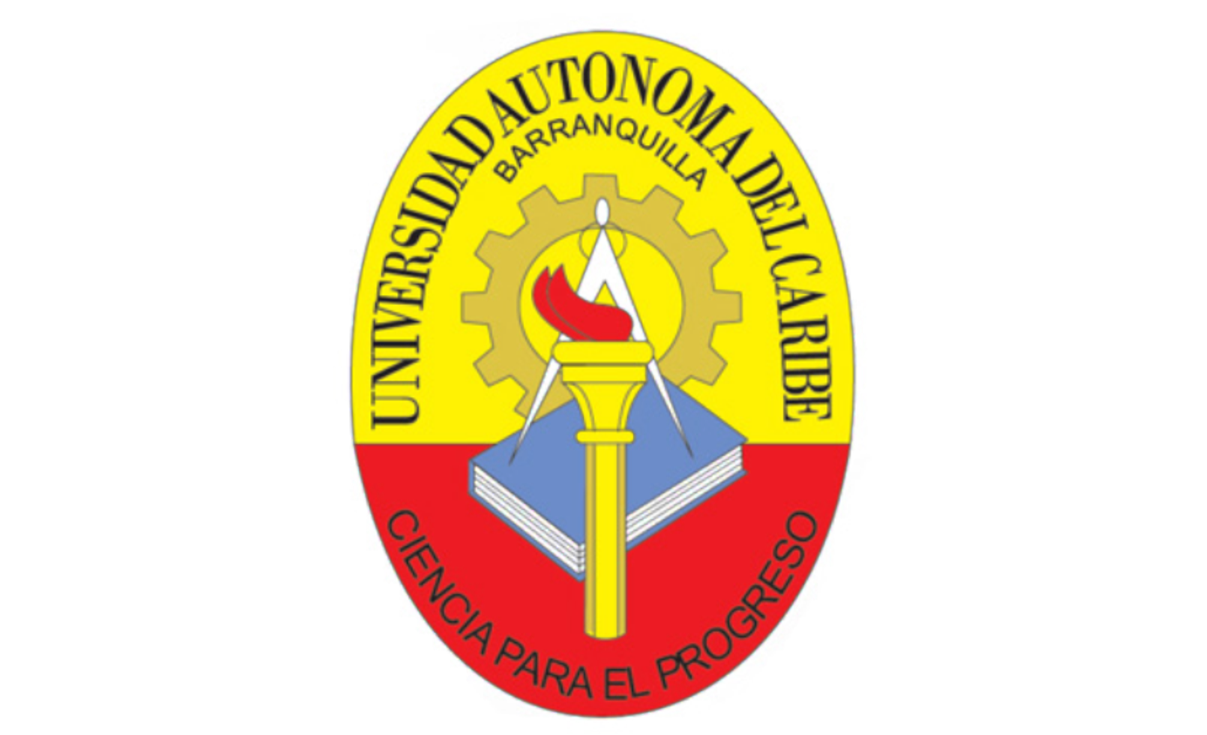
\includegraphics[scale=0.3]{uac}
\end{figure}


 \end{multicols} 

\vfill

 \begin{multicols}{2} 

\colorbox{ptctitle}{\color{white}\bfseries\sffamily Rectora Universidad Del Atlántico :}

ANA SOFÍA MESA DE CUERVO

\colorbox{ptctitle}{\color{white}\bfseries\sffamily Rector Universidad Autónoma Del Caribe :}

\uppercase{ Ramses Vargas Lamadrid}

 \end{multicols} 

\vfill

\colorbox{ptctitle}{\color{white}\bfseries\sffamily VICERECTOR ADMINISTRATIVO Y FINANCIERO:}

FREDDY DÍAZ MENDOZA\vfill

\colorbox{ptctitle}{\color{white}\bfseries\sffamily VICERECTOR DE DOCENCIA:}

REMBERTO DE LA HOZ REYES \vfill

\colorbox{ptctitle}{\color{white}\bfseries\sffamily VICERECTORA DE INVESTIGACIÓN, EXTENSIÓN Y PROYECCIÓN SOCIAL:}

RAFAELA VOS OBESO \vfill

\colorbox{ptctitle}{\color{white}\bfseries\sffamily DECANO FACULTAD DE CIENCIAS BÁSICAS :}

LUIS CARLOS GUTIÉRREZ MORENO\vfill\vspace{3cm}

\textsf{El material de esta publicación no puede ser reproducido sin
la autorización de los autores y editores. La responsabilidad del
contenido de este texto corresponde a sus autores.} \vfill

\begin{center}
\copyright UNIVERSIDAD DEL ATLÁNTICO BARRANQUILLA - COLOMBIA 2014 
\par\end{center}

\begin{center}
\copyright UNIVERSIDAD AUTÓNOMA DEL CARIBE BARRANQUILLA - COLOMBIA
2014
\par\end{center}

\begin{center}
\vfill\newpage
\par\end{center}

\begin{mdframed}[backgroundcolor=ptctitle,hidealllines=true]
\parbox[t]{\dimexpr\textwidth-2\fboxsep\relax}{  \color{white}\bfseries\sffamily  COMITÉ LATINOAMERICANO DE MATEMÁTICA EDUCATIVA }
\end{mdframed}

\colorbox{ptctitle}{\color{white}\bfseries\sffamily Comisión Directiva Presidenta:}
Claudia Lara Galo (Guatemala) 

\colorbox{ptctitle}{\color{white}\bfseries\sffamily Secretaria:}
Cecilia Crespo Crespo (Argentina)

\colorbox{ptctitle}{\color{white}\bfseries\sffamily Tesorera:} Elizabeth
Mariscal Vallarta (México)

\begin{mdframed}[backgroundcolor=ptctitle,hidealllines=true, rightmargin=0.5\textwidth ]
\parbox[t]{\dimexpr\textwidth-2\fboxsep\relax}{ \color{white}\bfseries\sffamily  Vocales: }
\end{mdframed}

\colorbox{ptctitle}{\color{white}\bfseries\sffamily Caribe:} Ángela
Martin (República Dominicana)

\colorbox{ptctitle}{\color{white}\bfseries\sffamily Centroamérica: }
Edison De Faria (Costa Rica)

\colorbox{ptctitle}{\color{white}\bfseries\sffamily Norteamérica: }
Marcela Ferrari (México)

\colorbox{ptctitle}{\color{white}\bfseries\sffamily Sudamérica: }
Patricia Lestón (Argentina)

\begin{mdframed}[backgroundcolor=ptctitle,hidealllines=true]
\parbox[t]{\dimexpr\textwidth-2\fboxsep\relax}{   \color{white}\bfseries\sffamily  COMITÉ NACIONAL ORGANIZADOR}
\end{mdframed}

\begin{mdframed}[backgroundcolor=ptctitle,hidealllines=true, rightmargin=0.5\textwidth]
\parbox[t]{\dimexpr\textwidth-2\fboxsep\relax}{   \color{white}\bfseries\sffamily  Coordinadores: }
\end{mdframed}

Alejandro Urieles G.

Blanca Peralta

Jorge Rodríguez C.

\begin{mdframed}[backgroundcolor=ptctitle,hidealllines=true, rightmargin=0.5\textwidth]
\parbox[t]{\dimexpr\textwidth-2\fboxsep\relax}{  \color{white}\bfseries\sffamily  Miembros: }
\end{mdframed}

 \begin{multicols}{2} 

Angélica Arroyo

Sonia Balbuena

Karina García

Alirio Gerardino

Antálcides Olivo

María José Ortega

Ramiro Peña

Jorge Robinson

Julio Romero

Lesly Salas

Diana Vargas

Gabriel Vergara

Ludwing Villa

Alejandro Villareal

Alexander Gutierrez

Freddy Molina

Eduardo Martinez

Harold Villamil

 \end{multicols} 

\newpage

\begin{mdframed}[backgroundcolor=ptctitle,hidealllines=true]
\parbox[t]{\dimexpr\textwidth-2\fboxsep\relax}{  \color{white}\bfseries\sffamily  COMITÉ 
EVALUADOR}
\end{mdframed}

 \begin{multicols}{2} 

\colorbox{ptctitle}{\color{white}\bfseries\sffamily Argentina : } 

Adriana Engler 

Alejandro Lois 

Ana María Mántica

Aníbal Moreno

Carlos Grande

Carmen Torrente

Cecilia Crespo Crespo

Cecilia Elguero

Cesar Fernandez 

Christiane Ponteville

Claudia Minaard 

Cristina Arceo

Cristina Camós

Daniela Müller

Daniela Reyes

Daniela Veiga

Diana Patricia Sureda

Elisa Oliva

Graciela Benzal

Haydeé Blanco

José Luis Rey

Leonor Carvajal

Liber Aparisi 

Lidia Esper

Lilian Cadoche 

Liliana Homilka

Liliana Milevicich

Lisa Holgado

Lucía Rodríguez Montelongo 

Mabel Alicia Slavin

Mabel Rodríguez

Malva Alberto 

Marcel Pochulu 

Margarita Veliz 

María Angélica Pérez de del Negro

María de los Angeles Fanaro

María Elina Vergara 

María Inés Ciando 

María Rosa Rodríguez de Estofán

Marta Adriana Correa Zeballos 

Marta Fierro Marta Inés Marcilla

Miguel Albione 

Mirta Débora Chan

Mónica García Zatti 

Ménica Micelli 

Noemí Geromini 

Nora Inés Lerman 

Patricia Fogliatti 

Patricia Lestón 

Patricia Villalonga de García 

Pedro Tomas Cohene 

Pierina Lanza 

Rita Otero

Sabrina Alarcon

Silvia Del Puerto 

Silvia Tajeyan 

Silvia Vrancken 

Sonia Ballico 

Susana González de Galindo

Susana Mercau 

Teresa Braicovich

Vicente Messina 

Viviana Carolina Llanos

\colorbox{ptctitle}{\color{white}\bfseries\sffamily Brasil : } 

Adlai Ralph 

Aliñe Silva de Bona 

Ana Paula Malheiros 

Claudia Liset Oliveira Groenwald

Gabriela Barbosa 

Marger Ventura 

Marlene Dias 

Plinto Moreira

\colorbox{ptctitle}{\color{white}\bfseries\sffamily Chile : } 

Daniela Soto 

Elizabeth Montoya 

Jaime Mena 

Jorge Avila Contreras 

Leonora Díaz 

Marcela Parraguez 

Mauricio Herrera

Patricia Vásquez Saldías

Pilar Alejandra Peña Rincón 

Soledad Montoya

\colorbox{ptctitle}{\color{white}\bfseries\sffamily Colombia : } 

Hilda Salgado 

Jhony Villa

\colorbox{ptctitle}{\color{white}\bfseries\sffamily Costa Rica : }

Anabelle Castro Castro

Edison De Faria 

\colorbox{ptctitle}{\color{white}\bfseries\sffamily Cuba : }

Aida María Torres

Alfonso Anelys Vargas Ricardo

Antonio Martínez Fonseca 

Elpidio López

Elsa Ramírez García 

Eugenio Carlos Rodríguez 

Iván Juan Valido González 

Luis A. Perfetti Villamil 

Marcelino González 

Mario Estrada Doallo 

Olga Lidia Pérez González

Osvaldo Rojas Velázquez 

Pedro Castañeda Porras 

Rafael Chaviano Conde 

Rafael Jiménez Martínez 

Ricardo Sánchez Casanova

Rosa Vázquez Cedeño

\colorbox{ptctitle}{\color{white}\bfseries\sffamily España: } 

José Carrillo Yañez 

Josefina Marta Marcolini Bernardi 

Tomás Ortega del Rincón

\colorbox{ptctitle}{\color{white}\bfseries\sffamily Grecia : }

Kyriakos Petakos 

\colorbox{ptctitle}{\color{white}\bfseries\sffamily Guatemala  : }

Claudia Lara Galo

\colorbox{ptctitle}{\color{white}\bfseries\sffamily Italia : }

Mariangela Borillo 

\colorbox{ptctitle}{\color{white}\bfseries\sffamily México : } 

Adriana Gómez Reyes 

Agustín Grijalva Alberto Camacho

Alejandro Rosas Mendoza

Alfonso Escorza Morales 

Alian Takeshi de la Cruz Oliva 

Alma Rosa Pérez 

Ana María Ojeda Salazar 

Ana Maria Olazabal Carpió

Araceli Rotaeche 

Bertha Ivonne Sánchez Luján

Carlos Oropeza Legorreta 

Catalina Navarro Sandoval 

Claudia Flores Estrada 

Crisólogo Dolores 

Eddie Aparicio 

Eduardo Miranda Montoya

Elena Nesterova 

Enrique Gómez Otero 

Erika Canché Góngora

Evelia Reséndiz 

Florencia Rodríguez 

Francisco Cordero Osorio 

Gabriela Buendía Abalos

Gisela Montiel 

Gustavo Martínez Sierra

Hipólito Hernández Pérez 

Isabel Tuyuc Sánchez

Ismael Arcos 

Javier Lezama

Jesús Salinas 

José Carlos Cortés Zabala

José Marcos López Mojica 

José Trujillo Torres 

Josefina Criberio Díaz 

Juan Adolfo Alvarez Martínez 

Juan de Dios Viramontes 

Julio Moisés Sánchez Barrera 

Landy Elena Sosa Moguel 

Leopoldo Zúñiga 

Leticia Sosa 

Liliana Suárez Téllez 

Marco Hernández Rodríguez 

Maria Guadalupe Cabañas Sánchez 

María Guadalupe Simón 

María Patricia Colin Uribe 

María del Socorro García 

Mayra Báez 

Miguel Solís Esquinca 

Miriam Martínez Vázquez 

Norma Gutiérrez Rodríguez 

Rebeca Flores 

Reynario Yudistire Cardona López 

Ricardo Cantoral Uriza 

Rogelio Ramos Carranza 

Rosa Isela Vázquez Camacho 

Rosa María Farfán Márquez

Ruth Rodríguez

Santiago Velázquez Bustamante 

Silvia Ibarra Olmos 

Silvia Maffey García 

Víctor Larios Osorio

Virginia Rivera Lara 

\colorbox{ptctitle}{\color{white}\bfseries\sffamily Panamá : }

Analida Ardila 

Germán Luis Beitía 

Héctor Osorio Abrego 

Luis Moreno Chadler 

\colorbox{ptctitle}{\color{white}\bfseries\sffamily República Dominicana: }

Ángela Martin

\colorbox{ptctitle}{\color{white}\bfseries\sffamily Uruguay : }

Cristina Ochoviet

Mario Dalcín Mónica Olave 

\colorbox{ptctitle}{\color{white}\bfseries\sffamily Venezuela : } 

Mario Ameche Alvarado

Sandra Castillo

Walter Beyer 

Yolanda Serres

\end{multicols}

}
%\end{multicols}
\vfill\newpage
{\color{white}
\bfseries

\begin{mdframed}[backgroundcolor=ptctitle,hidealllines=true]
\parbox[t]{\dimexpr\textwidth-2\fboxsep\relax}{  \color{white}\bfseries\sffamily  PRESENTACIÓN }
\end{mdframed}

Es para nosotros un verdadero honor, ser los anfitriones de la {\bf VIGÉSIMA OCTAVA REUNIÓN LATINOAMERICANA DE MATEMÁTICA EDUCATIVA, RELME 28,}
a realizarse en Barranquilla, Colombia, del 28 de julio al 1 de agosto
de 2014. Colombia fue sede de la Relme 12 en el año 1998, en la ciudad
de Bogotá. Hoy, de nuevo somos la sede de tan importante reunión y
quisimos que, al igual que aquel entonces, tener una asistencia masiva
de profesores, estudiantes, doctores, investigadores y en general
de personas preocupadas por la Matemática Educativa en América y el
mundo. Esperamos que puedan encontrar espacios en donde no solo establezcamos
alianzas o compartamos preocupaciones; deseamos que tengan la posibilidad
de tejer afectos, esperanzas, esfuerzos e ideas en pro de una mejor
educación para los pueblos de América.

Con la alegría que caracteriza a los barranquilleros, les damos la
bienvenida a nuestra ciudad para hacer de este sueño una realidad. 

\begin{center}
 \large \bfseries\sffamily  Comité Nacional Organizador RELME 28 
\end{center}

Hemos logrado entusiasmar a colegas de diversos países que podrán
participar de las cerca de 760 actividades programadas: Más de 90
invitadas y alrededor de 680 aceptadas por el comité evaluador.

\begin{multicols}{2}

Conferencias plenarias: 2 

Conferencias especiales: 46 

Cursos cortos: 44 

Mesas redondas: 3

Grupos de trabajo y discusión: 6 

Reportes de investigación: 347 

Comunicaciones breves: 229 

Talleres: 48 

Posters: 42

\end{multicols}

En el caso de las conferencias plenarias, conferencias especiales
y los cursos cortos, nosotros, el comité organizador, invitamos a
destacados especialistas brindando un espacio a quienes han desarrollado
con tesón, ilusión y alegría, trabajos en distintas áreas. Para el
resto de propuestas, siguiendo la tradición de RELME, el comité académico
envió a dos árbitros cada uno de los trabajos. En el caso que no hubiera
acuerdo entre las opiniones de éstos, la propuesta era enviada a un
tercero quien decidía sobre la aceptación o no de la misma.

Tenemos la inmensa oportunidad de contar con la presencia, palabra
y entusiasmo de profesores de todos los niveles educativos, de diversas
formaciones académicas y que provienen de los más bellos parajes de
nuestro continente, así nos acompañan: Argentina, Brasil, Chile, Colombia,
Costa Rica, Cuba, Dinamarca, España, Estados Unidos, Guatemala, México,
Panamá, Perú, Portugal, Puerto Rico, República Dominicana, Uruguay
y Venezuela. 

 }\newpage\newpage
%\maketitle

\let\myclearpage\clearpage\tableofcontents{}\let\myclearpage\relax\newpage{}

%\pagecolor{ptcbackground}
\pagestyle{headings}
\nocite{*}
\fontsize{7}{8}\selectfont
%\setlength{\baselineskip}{5pt}
\pagecolor{white} 
\mainmatter 

\pagecolor{white} \mainmatter \pagestyle{headings}

\chapter{Conferencias Especiales} 
\chaptertoc
\twocolumn
\balance


\section{INVESTIGACIÓN EN EDUCACIÓN MATEMÁTICA Y LOS RETOS DE LA INCLUSIÓN
EN AMERICA LATINA}

\begin{datos}
Paola Valero\\
Universidad de Aalborg,\\
Dinamarca \\
\hfill paola@learning.aau.dk
\end{datos}

La educación matemática es el pilar de economías competitivas para
alcanzar el crecimiento y bienestar económicos. Este enunciado ilustra
la racionalidad sobre la función de la educación matemática para el
trabajo y la economía. Investigación que sirva, con evidencias contundentes,
y que sí asegure el éxito escolar es lo que piden administradores,
políticos y el público en general. En esta plenaria me interesa criticar
esta perspectiva con preguntas como: ¿Cuáles han sido los objetos
de estudio de la educación matemática? ¿Cómo la investigación en educación
matemática contribuye a un colonialismo cultural que se disfraza detrás
de la neutralidad de las matemáticas? Finalmente, señalaré estrategias
de investigación para repensar qué papel puede jugar la investigación
en educación matemática en enfrentar la exclusión sistemática de grandes
porciones de la población en el éxito educativo.


\section{FILOSOFÍA, MATEMÁTICAS Y EDUCACIÓN: UNA PERSPECTIVA HISTÓRICO-CULTURAL
EN EDUCACIÓN MATEMÁTICA}

\begin{datos}
Gilberto Obando Zapata\\
Universidad de Antioquia, \\
 Colombia,\\
\hfill gilberto.obando@udea.edu.co 
\end{datos}

En esta conferencia, sobre la base de planteamientos epistemológicos
derivados de la teoría de la actividad, en primer lugar se argumenta
en favor de una postura sobre el conocimiento matemático que posiciona
los procesos individuales y sociales de su constitución como polos
de una dualidad dialéctica mediada por los sistemas de prácticas socialmente
compartidos. Con base en estos planteamientos, y tomando en consideración
la noción de configuración epistémica, en segundo lugar, se presenta
una caracterización de los sistemas de práctica matemática (objetos
y conceptos, instrumentos y procedimientos, problemas por resolver),
aportando elementos teóricos y metodológicos para el estudio de la
actividad matemática de los individuos en condiciones institucionales
específicas.


\section{COLONIZACIÓN Y MATEMÁTICAS ESCOLARES. UNA MIRADA HISTÓRICO CULTURAL
A LA EDUCACIÓN MATEMÁTICA}

\begin{datos}

Paola Valero$^{1}$, Gloria García$^{2}$.

$^{1}$Universidad de Aalborg, $^{2}$Universidad Pedagógica Nacional
de Colombia,

$^{1}$Dinamarca, $^{2}$Colombia,

paola@learning.aau.dk; gloriag@pedagogica.edu.co

\end{datos}

Los estudios histórico-culturales que hemos realizado nos permiten
pensar el funcionamiento del currículo de matemáticas como una tecnologías
de gobierno. Estas tecnologías fabrican al sujeto racional, objetivo,
universal que realiza las promesas del ciudadano cosmopolita Moderno.
A través del estudio de la inserción histórica de las matemáticas
escolares en el proyecto colonizador y sus mutaciones en el siglo
20, mostramos como el currículo de matemáticas opera para efectuar
la entrada de Colombia en la promesa del desarrollo. La pregunta que
surge es si es posible mantener una visión cándida del supuesto “empoderamiento”
que se le atribuye a las matemáticas escolares cuando su constitución
histórico-cultural se fundamenta en la exclusión de proyectos de subjetividad
diferentes a los de la Modernidad Europea y Norteamericana.


\section{UNA PERTURBACIÓN VÍA INTELIGENCIAS MÚLTIPLES DEL ENFOQUE DE J. D.
GODINO SOBRE LA COGNICIÓN MATEMÁTICA: REPORTE DE UN ESTUDIO DE CASO
RELACIONADO CON ALGUNOS TEMAS DE ANÁLISIS MATEMÁTICO}

\begin{datos}
Universidad Simón Bolívar,  \\
Venezuela,\\
\hfill  yquintana@usb.ve 
\end{datos}

En esta charla se presentarán algunos resultados de un estudio reciente
sobre el uso de los sistemas de representación semiótica como herramienta
para determinar los significados institucionales y personales contenidos
en algunos temas de Análisis Matemático de Licenciaturas de Matemática
y Educación Matemática de Universidades venezolanas. La idea central
de este estudio es perturbar el enfoque de cognición matemática propuesto
por J. D. Godino (2003) usando como plataforma cognitiva a la Teoría
de Inteligencias Múltiples -en lugar de la Teoría Antropológica-,
con el objeto de identificar posibles conflictos semióticos presentes
en el proceso de enseñanza-aprendizaje de temas de Análisis Matemático. 


\section{LA PEDAGOGÍA SOCIAL Y SUS APORTES A LA ENSEÑANZA DE LA MATEMÁTICA}

\begin{datos}
Miledys Tavárez Marzán\\
Facultad de Educación, Universidad Autónoma de Santo Domingo,   \\
Republica Dominicana,\\
\hfill  miledyst@gmail.com 
\end{datos}

Al relacionar Pedagogía Social y Matemática educativa, es por su vinculación
de forma directa con la didáctica y la vida social. Muchos han querido
soslayar estas cercanías y es necesario que educadores matemáticos,
investigadores e investigadoras trabajemos con mayor esfuerzo esta
relación para que los aprendices de la matemática puedan valorar su
potencia en la sociedad. Matemática, vida y realidad comulgan en el
intelecto humano para entender su mundo y su accionar, la pedagogía
social surge para fortalecer la participación derribando prejuicios
sociales, la matemática se hace necesaria para los procesos actuales
del ser humano, urge involucrar a las mayorías en su aprendizaje.


\section{TECNOLOGÍAS NO CURRÍCULO DE MATEMÁTICA}

\begin{datos}
Claudia Lisete Oliveira Groenwald\\
Universidade Luterana do Brasil, ULBRA   \\
Brasil,\\
\hfill  claudiag1959@yahoo.com.br
\end{datos}

Esta conferência apresenta os resultados de pesquisa do projeto Inovando
o Currículo de Matemática através da Incorporação das Tecnologias.
A investigação está associada ao convênio firmado entre a Universidade
de La Laguna (ULL), em Tenerife, Espanha, com o grupo de Tecnologias
Educacionais e a Universidade Luterana do Brasil, com o Grupo de Estudos
Curriculares em Educação Matemática (GECEM), do Programa de Pós-Graduação
em Ensino de Ciências e Matemática (PPGECIM). Apresenta-se o SIENA
- sistema integrado de ensino e aprendizagem, que é um sistema inteligente
para o desenvolvimento do processo de ensino e aprendizagem de um
conteúdo qualquer, para qualquer nível de ensino. Todo trabalho no
SIENA possui as seguintes ações: grafo com o conteúdo a ser desenvolvido,
banco de questões para os testes adaptativos e sequências didáticas
para cada conceito do grafo. O sistema possui duas opções de uso:
a primeira serve para o aluno estudar os conteúdos do grafo planificado
e realizar o teste, para verificar quais são seus conhecimentos sobre
determinados conteúdos; a segunda opção oportuniza, ao aluno, realizar
o teste e estudar os conceitos nos quais apresentou dificuldades,
sendo possível uma recuperação individualizada dos conteúdos nos quais
não conseguiu superar a média estipulada como necessária para avançar.
O sistema SIENA permite estudos individualizados e, em grupos de estudos,
possibilitando tanto a recuperação individualizada de conteúdos como
a aprendizagem através da cooperação e colaboração entre os pares.
Entende-se que os educadores têm como desafio, descobrir maneiras
diferentes de ensinar a mesma coisa, pois os estudantes têm ritmos
e históricos variados, além disso, o sistema educacional, historicamente,
é projetado igualmente para todos os estudantes, de forma que o aluno
deve adaptar-se em um contexto educacional definido. O professor necessita,
nos dias atuais, questionar a abordagem do conteúdo, devendo despertar
a curiosidade do educando e demonstrar sua utilização em diferentes
situações da vida real. Assim um dos desafios que os professores encontram,
em sala de aula, é a identificação das dificuldades individuais dos
alunos. Nesse sentido, o uso de recursos informáticos pode influenciar
beneficamente quando utilizados como suporte ao trabalho docente.
Em uma sociedade de bases tecnológicas, com mudanças contínuas, não
é mais possível desprezar o potencial pedagógico que as Tecnologias
de Informação e Comunicação (TIC) apresentam quando incorporadas à
educação. Assim, o computador é um instrumento pertinente no processo
de ensino e aprendizagem, cabendo à escola utilizá-lo de forma coerente
com uma proposta pedagógica atual e comprometida com uma aprendizagem
significativa.


\section{¿QUÉ PODEMOS APRENDER DE LOS PAÍSES DE ALTO RENDIMIENTO EN LAS MATEMÁTICAS?}

\begin{datos}
Patrick Scott\\
Universidad Estatal de Nuevo México (Emérito)   \\
\hfill  pscott@nmsu.edu
\end{datos}

Japón, Corea, China, Finlandia y Polonia han recibido mucha fama por
su éxito en las pruebas internacionales de PISA. ¿Cuáles son algunas
de las características demográficas de dichos países y cómo se comparan
con los países de América Latina? ¿Cómo son sus programas de matemáticas?
¿Qué son algunos de los aspectos principales de sus sistemas educativos?
¿Cuáles son algunos de dichos aspectos son los principales en su éxito
en pruebas internacionales? ¿Cómo se comparan los aspectos educativos
principales de dichos países con aquellos de los países de América
Latina? ¿Qué debemos aprender de sus experiencia? 


\section{LA HISTORIA DE LAS MATEMÁTICAS EN EL CONOCIMIENTO DIDÁCTICO DEL CONTENIDO
MATEMÁTICO DEL PROFESOR DE MATEMÁTICAS }

\begin{datos}
Edgar Alberto Guacaneme Suárez – Lyda Constanza Mora Mendieta\\
Universidad Pedagógica Nacional,\\ Colombia,  \\
\hfill  guacaneme@pedagogica.edu.co – lmendieta@pedagogica.edu.co
\end{datos}

El vínculo entre la Historia de las Matemáticas {[}HM{]} y el conocimiento
del profesor de Matemáticas {[}CPM{]} exhibe interesantes matices
cuando se analiza la intervención de la HM en el conocimiento didáctico
del contenido matemático {[}CDCM{]}, entendido como un componente
del CPM. Tales matices viran de manera singular cuando, más allá de
posiciones discursivas, se investiga sobre las especificidades de
la introducción factual del conocimiento histórico en cursos de didácticas
específicas de las Matemáticas, a través de los cuales se procura
favorecer el CDCM con la HM. Esta condición impone, al formador de
profesores, altas exigencias respecto de su conocimiento.


\section{LA EVALUACIÓN DEL DOMINIO AFECTIVO EN MATEMÁTICAS. IDEAS Y CONCEPCIONES
DE LOS PROFESORES DE MATEMÁTICAS.}

\begin{datos}
Janeth A. Cárdenas Lizarazo\\
Universidad de Extremadur,\\ España,  \\
\hfill  jacardenasl@unex.es
\end{datos}

Diversas investigaciones constatan la importancia e influencia que
tienen los aspectos del dominio afectivo en el aprendizaje y la enseñanza
de las matemáticas. En algunas prácticas de evaluación, el profesor
evalúa lo actitudinal en los estudiantes, a partir de unas pautas
de comportamiento que visualiza en ellos. Cuando dichas pautas de
comportamiento siguen patrones negativos, se siguen procesos formativos,
a partir de sugerencias que se dan a los estudiantes y a los padres
de familia, y en caso de ser necesario se sanciona a través de la
calificación; rara vez se buscan respuestas en el dominio afectivo
de los estudiantes.


\section{CONFERENCIA ESPECIAL UNA “BUENA CLASE” DE MATEMÁTICAS: ¿QUÉ DEBE
ENFRENTAR ACTUALMENTE UN DOCENTE?}

\begin{datos}
Harold Castillo Sánchez\\
Pontificia Universidad Javeriana. Seccional Cali,\\ Colombia,  \\
\hfill  hcastillo@javerianacali.edu.co
\end{datos}

¿Qué han aportado las diversas investigaciones en didáctica de las
matemáticas para cuestionar las planificar, realizar y evaluar una
“buena clase”? ¿Cómo se determina, a la luz de nuevas propuestas didácticas,
que se ha realizado una “buena clase”?. En esta ponencia se presentarán
diversas posturas resultado de investigaciones en didáctica de las
matemáticas con el objetivo de reflexionar, y crear un espacio de
reflexión, sobre lo que, como docente de matemáticas, se debe considerar
para afrontar un curso o asignatura de matemáticas en cualquier nivel
educativo.


\section{DIFICULTADES EN EL APRENDIZAJE DE LA MATEMÁTICA}

\begin{datos}
Luis Roberto Moreno Chandler\\
CAIDDAM Panamá - Universidad de Panamá,\\
\hfill  LuisMo@gmail.com   luisro25@hotmail.com
\end{datos}

Las dificultades en el aprendizaje de la matemática constituyen un
tema que aparece con frecuencia en los discursos docentes y en resultados
de investigadores en matemática educativa. En muchos casos es evidente
el manejo informal del tema y el desconocimiento de una amplia gama
de resultados e información estructurada científicamente producto
del trabajo de profesionales de diversas disciplinas científicas interesado
en el tema. Nos proponemos revisar y compartir algunos aspectos fundamentales
para el estudio, investigación y atención de las DAM, es por ello
que abordaremos los siguientes aspectos: aproximación conceptual,
factores, teorías explicativas, diagnóstico, efectos y sugerencias
para su intervención. 


\section{\uppercase{ La variable aleatoria: un experimento de enseñanza en
el curso de probabilidad}}

\begin{datos}
Mora Rodríguez Yeferson Ferney - Parodi Garrido Karla Paola\\
Universidad Pedagógica Nacional,\\ Colombia,\\
\hfill  yefri123@hotmail.com – mgkarlaparodi@gmail.com 
\end{datos}

En este trabajo, inscrito en la línea de Educación Estadística de
la Universidad Pedagógica Nacional, se diseñaron dos talleres para
posibilitar el aprendizaje de la distribución binomial e hipergeométrica,
por medio de métodos no magistrales, que a su vez proporcionaran datos
que permitieran clasificar el nivel estadístico de los estudiantes
del curso de probabilidad. Se llegó a las conclusiones, por medio
de estadísticas, de que el mayor porcentaje de los estudiantes corresponden
al nivel de pensamiento estadístico y que los talleres diseñados fueron
funcionales para este tipo de experimentos. 


\section{UN MODELO DEL CONOCIMIENTO BASE PARA LA ENSEÑANZA DEL FORMADOR DE
PROFESORES DE MATEMÁTICAS ENCARGADO DEL COMPONENTE DIDÁCTICO}

\begin{datos}
Andrea Milena Beltrán Beltrán, Fernando Lázaro Luna, Lyda Constanza Mora Mendieta\\
Universidad Pedagógica Nacional,\\ Colombia,\\
 \hfill mdma\_abeltran343@pedagogica.edu.co; mdma\_wlazaro526@pedagogica.edu.co;\\  \hfill lmendieta@pedagogica.edu.co 
\end{datos}

En la conferencia que se propone se presenta un modelo de lo que se
considera es el Conocimiento Profesional del Formador de Profesores
de Matemáticas (CPFPM), en particular, de aquel profesional encargado
de la enseñanza del componente Didáctico. Dicho modelo, es resultado
de: 1) un estudio de caso llevado a cabo en la Universidad Pedagógica
Nacional (Bogotá, D.C., Colombia) y 2) un proceso análogo desarrollado
a partir de la propuesta planteada por Shulman (1986) con relación
al conocimiento profesional del profesor y, una adaptación que hace
Pinto (2010) para el caso particular del conocimiento del profesor
de matemáticas. 

\setcounter{section}{14}


\section{EL NECESARIO PERO DIFÍCIL DIÁLOGO ENTRE LA MATEMÁTICA ESCOLAR Y LA
REALIDAD (DE LOS ESTUDIANTES)}

\begin{datos}
Hugo Parra S.\\
Universidad del Zulia,\\ Venezuela,\\
\hfill hps1710@yahoo.es \end{datos}

Abordaremos la vinculación de las matemáticas escolares con la realidad,
ya que es una exigencia tanto desde el ámbito institucional como del
académico. Esta vinculación supone experiencias significativas para
los estudiantes que sólo será posible si se establece un diálogo entre
la matemática escolar y las diferentes prácticas sociales – cotidianas
o no - asociadas a las matemáticas. Para ello se debe reconsiderar
los actores y su rol en los procesos de enseñanza y aprendizaje. Además,
exige de la institución escolar traspasar sus muros e ir al encuentro
de las diferentes prácticas sociales de la matemática externas a ella. 


\section{CONFERENCIA: SIGNIFICADO FILOSÓFICO DEL CERO MAYA: NIK}

\begin{datos}
José Mucia Batz.\\
 Guatemala.CA,\\
\hfill batz.lem@gmail.com \end{datos}

NIK: El cero forma parte de los tres símbolos numéricos básicos para
el conteo vigesimal maya. Cosmovisión maya. El pensamiento maya es
circular a similitud del cosmos, por lo tanto el conteo también es
circular. Círculos numéricos. Conteo desde el cero hasta el diecinueve
es el primer círculo. El cero forma parte del ciclo y tiene la posición
de ser el principio y fin. La semilla cumple con los requisitos de
ser cero porque es el principio y fin. El día cero del calendario
maya es el día Ajaw. El punto cero en la vida es el nacimiento y la
muerte.


\section{DEFICIENCIAS EN LOS CONTENIDOS MATEMATICOS Y DIDÁCTICOS DE LOS PROFESORES
EN EJERCICIO EN REPÚBLICA DOMINICANA}

\begin{datos}
Carmen Evarista Matías de Rodríguez.\\
Universidad Autónoma de Santo Domingo,\\ República Dominicana,\\
\hfill evaristam@gmail.com \end{datos}

Se realiza un estudio de tipo exploratorio para identificar las deficiencias
en los contenidos matemáticos y didácticos de los profesores en ejercicio.
La muestra estuvo conformada por 48 estudiantes de la Maestría en
Didáctica de la Matemática, de la Facultad de Ciencias de la Educación
de la Universidad Autónoma de Santo Domingo, República Dominicana.
Identificando la detección de deficiencias como parte del proceso
de evaluación, el estudio se fundamenta teóricamente en los principios
de la evaluación del aprendizaje del carácter contingente de la evaluación
y el principio del equilibrio valorativo en la evaluación, así como
en las regularidades metodológicas para el desarrollo de la evaluación.
Los resultados muestran que es contradictorio que más de la mitad
de los profesores se siente completamente satisfechos con el trabajo
que realizan y que a la vez manifiesten que tienen dificultades con
el conocimiento de los conceptos fundamentales de la Didáctica y,
además, el 81.25\% tiene algunas o bastantes deficiencias lo que permite
indicar que los métodos de investigación para la profesionalización
de estos profesores deben estar dirigidos, en primera instancia, a
lograr en ellos el reconocimiento, de su propio nivel de desarrollo,
buscando el equilibrio evaluativo entre los profesores. 


\section{RETOS Y DILEMAS DE LA FORMACIÓN DEL PROFESORADO DE MATEMÁTICAS QUE
BUSCA DESARROLLO PROFESIONAL}

\begin{datos}
Edelmira Badillo.\\
Departament de Didàctica de les Matemàtiques i de les CCEE. Universitat Autónoma de Barcelona,\\ España,\\
\hfill evaristam@gmail.com \end{datos}

En esta conferencia compartiré reflexiones realizadas, desde mi experiencia
como maestra de matemáticas, formadora de maestros e investigadora,
sobre los elementos esenciales de los modelos de formación del profesorado
de matemáticas. Un recorrido por los antecedentes de esta línea de
investigación desvelará retos y dilemas sobre las características
de la formación que promueven auténtico desarrollo profesional. Finalmente
compartiré instrumentos formativos que estamos implementando para
ayudar al profesorado a identificar los elementos relevantes de una
práctica matemática de aula; a conectar la interacción con los aprendizajes
de sus estudiantes y a usar sus conocimientos para reflexionar sobre
su práctica y mejorarla. 


\section{A LITERATURA COMO MOTIVADORA PARA O ENSINO DE MATEMÁTICA: UM OLHAR
SOBRE AS OBRAS DE LEWIS CARROLL}

\begin{datos}
Rafael Montoito.\\
Instituto Federal Sul-Rio-Grandense (IFSUL, Campus Pelotas),\\ Brasil,\\
\hfill xmontoito@ig.com.br \end{datos}

Aliando imaginação e fantasia às aulas de matemática, a literatura
pode favorecer o ambiente de ensino e servir para discutir conteúdos
que, às vezes, aparecem nos livros didáticos de uma maneira puramente
conceitual. Vários estudos teóricos têm falado, também, sobre a necessidade
atual de os alunos aprenderem a ler, escrever e argumentar matematicamente,
o que é possível ser trabalhado com atividades que abordam a língua
materna e os conceitos e conteúdos matemáticos. Dentre os autores
cujos livros servem a essas propostas, destacamos as obras de Lewis
Carroll, suas intenções como autor e suas opiniões sobre a educação
e o ensino.


\section{\uppercase{ La escuela, el aula, la enseñanza de la matemática.
Un recorrido a través de la historia}}

\begin{datos}
Cecilia Crespo Crespo.\\
Instituto Superior del Profesorado “Dr. Joaquín V. González”,\\ Buenos Aires (Argentina),\\
\hfill crccrespo@gmail.com \end{datos}

La matemática ha sido considerada por distintas culturas como disciplina
necesaria para explicar y predecir situaciones y fenómenos de la naturaleza,
lo económico y lo social. Este trabajo presenta un recorrido a lo
largo de la historia describiendo el espacio en el que tenía lugar
la enseñanza de la matemática en diversos escenarios socioculturales
y su relación con la manera en la que se transmitía o construía el
conocimiento matemático. Intentaremos comprender que el aula actual
tiene un pasado y que emergió en respuesta a desafíos específicos
y siguen teniendo algunos de sus significados originales. 


\section{EDUCACIÓN MATEMÁTICA CRÍTICA Y EDUCACIÓN RELIGIOSA FEMENINA: ¿PROYECTOS
INCOMPATIBLES?}

\begin{datos}
Edgar Johanni Angulo Oliveros, Claudia Salazar Amaya, \\ Jorge Edilson Solano Espitia.\\
Universidad Tecnológica de Bolívar- Universidad Pedagógica Nacional,\\ Colombia,\\
\hfill edgarangulo72@hotmail.com; csalazar@pedagogica.edu.co; \\ \hfill jorgesolanoespitia@gmail.com \end{datos}

En Educación Matemática es frecuente considerar el significado como
centro de los procesos de enseñanza y aprendizaje de las matemáticas
escolares y asociar éste a las comprensiones de los estudiantes sobre
los objetos de estudio. Este “centro” caracteriza los aprendizajes
que se esperan sean alcanzados. Sin embargo, nuestra investigación
pretende discutir que el “centro” de los procesos del aprendizaje
y la enseñanza de las matemáticas sea el significado, partiendo del
reconocimiento de la resonancia entre los significados que las estudiantes
le atribuyen a las matemáticas y los propósitos de un proyecto de
formación de una escuela privada, católica y femenina. 


\section{CLASIFICACIÓN DE LOS ARGUMENTOS PRODUCIDOS POR ESTUDIANTES QUE INGRESAN
A CARRERAS TÉCNICAS AL RESOLVER UNA TAREA DE GENERALIZACIÓN CON NÚMEROS
4-ESTELARES}

\begin{datos}
Miller Palacio Núñez \\
Escuela colombiana de Carreras Industriales,\\ Colombia,\\
\hfill milpal252000@gmail.com \end{datos}

El objetivo principal de esta conferencia es presentar los resultados
encontrados en un trabajo de grado de la Maestría en Docencia de la
Matemática, el cual tiene como propósito clasificar los argumentos
desarrollados por un grupo de estudiantes de primer semestre de universidad
al resolver una tarea relacionada con números 4-estelares. El análisis
de los argumentos logrados por los estudiantes se hace a partir del
modelo de Toulmin como unidad mínima de argumentación. Estos resultados
se clasifican de acuerdo a los garantes y las hipótesis planteadas
por ellos en cinco modelos de argumentación a partir de la expresión
general encontrada. 


\section{PROPUESTA DE FORMACIÓN POSGRADUAL EN EDUCACIÓN MATEMÁTICA SUSTENTADA
EN LA INVESTIGACIÓN. UNIVERSIDAD PEDAGÓGICA NACIONAL, BOGOTÁ (COLOMBIA)}

\begin{datos}
Leonor Camargo Uribe, María Nubia Soler-Álvarez \\
Universidad Pedagógica Nacional,\\ Colombia,\\
\hfill lcamargo@pedagogica.edu.co, nsoler@pedagogica.edu.co  \end{datos}

Esta conferencia presenta a la comunidad internacional una propuesta
de formación que se viene desarrollando desde el año 2008 en el programa
de Maestría en Docencia de la Matemática (MDM) de la Universidad Pedagógica
Nacional (Bogotá – Colombia), la cual se articula alrededor del desarrollo
de competencias investigativas e innovativas, con las cuales pretendemos
que nuestros egresados se incorporen al campo de conocimiento de la
educación matemática, se cualifiquen y contribuyan a la solución de
problemas propios del contexto colombiano. Esperamos que impulse el
intercambio académico de experiencias de formación postgradual y sirva
como referente de formación en otros países latinoamericanos.


\section{DIFICULTADES DE LOS ESTUDIANTES DE PROFESORADO EN RELACIÓN AL ÁLGEBRA}

\begin{datos}
Patricia Lestón. \\
Instituto Superior del Profesorado “Dr. Joaquín V. González”,\\ Argentina,\\
\hfill patricialeston@gmail.com  \end{datos}

El presente trabajo propone presentar algunas de las dificultades
que los estudiantes de Primer Año de Profesorado en Matemática evidencian
al enfrentar un primer curso de álgebra. Se analizaran algunas de
las problemáticas detectadas apoyados en la teoría socioepistemológica,
considerando las cuatro componentes de la construcción del conocimiento
matemático (social, didáctica, epistemológica y cognitiva). En base
a ese análisis y al estudio del discurso matemático escolar propio
del Instituto de Formación Docente que se toma como ejemplo, en este
caso, el Instituto Superior del Profesorado “Dr. J. V. González”;
se plantearan algunas ideas para el rediseño del curso.


\section{DESARROLLO PROFESIONAL DEL PROFESOR DE MATEMÁTICAS: ¿CURSOS, MAESTRÍAS,
O COLECTIVOS?}

\begin{datos}
Javier Lezama. \\
Instituto Politécnico Nacional,\\ México,\\
\hfill jlezamaipn@gmail.com \end{datos}

La experiencia de trabajo en las actividades que son reconocidas formalmente
como desarrolladoras del desempeño profesional del profesor de matemáticas,
tales como estudios de posgrado, cursos específicos en el campo disciplinar,
así como de reflexión didáctica y pedagógica la sobre docencia en
matemáticas, han dejado de lado la creación de colectivos de profesores
que de manera independiente y con espíritu profesional definan los
estándares de desempeño y analicen de manera crítica su actividad
docente para así hacer planteamientos alternativos e innovadores para
educar matemáticamente a la sociedad. En esta conferencia reflexionamos
sobre este tema. 


\section{LA EDUCACIÓN MATEMÁTICA EN EL MUNDO DE LA WEB 2.0}

\begin{datos}
Sandra L. Castillo V. \\
Universidad Nacional Experimental de Guayana,\\ Venezuela,\\
\hfill sandralilianacastillo@gmail.com  \end{datos}

Se pretende, con esta Conferencia Especial, establecer la importancia
que se debe otorgar al uso de las Tecnologías de Información y Comunicación
(TIC) en el área de la Educación Matemática particularmente con el
uso de herramientas como la WEB 2.0 y otras TIC en los procesos de
enseñanza y aprendizaje de las matemáticas y, a la vez, hacer una
reflexión crítica acerca de la práctica del docente de matemática
en tiempos de la Educación 2.0. Para ello se desarrollarán los siguientes
tópicos: Características de la educación 2.0. ¿Cómo se perfilan los
procesos de enseñanza y aprendizaje de la matemática dentro del mundo
de la WEB 2.0? ¿Se puede hablar de cambios en la manera de enseñar
y en la manera de aprender matemática mediante la utilización de la
WEB 2.0? Rol del docente de matemática en tiempos de la WEB 2.0 ¿Cómo
ha resultado ser la apropiación de los conocimientos matemáticos cuando
se hace uso de los elementos propios de la WEB 2.0? Finalmente, no
olvidemos que por mucha tecnología -moderna o no- que exista, el rol
del DOCENTE es primordial en todos los procesos involucrados en la
Educación Matemática sin menoscabo del ambiente y teniendo como protagonista
al ALUMNO.


\section{\uppercase{ Evaluación en el Aula y Matemática Educativa}}

\begin{datos}
Ángel Homero Flores Samaniego. \\
Colegio de Ciencias y Humanidades, UNAM,\\ México,\\
\hfill ahfs@unam.mx \end{datos}

La evaluación en el aula es la recolección de información pertinente
sobre el proceso de enseñanza-aprendizaje con miras a su mejora. Mientras
que la matemática educativa tiene como objetivo el estudio de los
procesos y la problemática que surgen en el ámbito de la enseñanza-aprendizaje
de la matemática con el objetivo de optimizar el aprendizaje de los
estudiantes. En la presente conferencia se abordará la evaluación
en el aula y su papel en la mejora del proceso de enseñanza-aprendizaje
a través de la retroalimentación y del uso de instrumentos de evaluación,
como instrumentos de investigación educativa en el aula.


\section{APRENDIZAJE DE LA MATEMÁTICA EN LÍNEA: LA EXPERIENCIA DE URUGUAY
CON LA PLATAFORMA ADAPTATIVA DE MATEMÁTICA}

\begin{datos}
Cristina Ochoviet. \\
Instituto de Perfeccionamiento y Estudios Superiores-Consejo de Formación en Educación,\\ Uruguay,\\
\hfill cristinaochoviet@gmail.com \end{datos}

La Plataforma Adaptativa de Matemática - bettermarks provee un ambiente
para aprender matemática en línea cuyo principal centro de atención
es el proceso de aprendizaje. Combina las potencialidades de los medios
digitales con una adecuada selección de contenidos y actividades matemáticas.
La retroalimentación que se brinda al estudiante es personalizada
y depende de lo que este va ingresando en las distintas etapas de
la resolución de una tarea, de ahí que hablemos de adaptividad. En
esta comunicación se presentará el entorno, focalizándonos en los
distintos tipos de ejercicios e interacciones que se ofrecen a los
estudiantes.


\section{CONOCIMIENTO SOBRE EL CONCEPTO DE FRACCIÓN DEL PROFESOR DE MATEMÁTICAS
DE SECUNDARIA}

\begin{datos}
Guadalupe Cabañas-Sánchez. \\
Universidad Autónoma de Guerrero,\\ México,\\
\hfill gcabanas@uagro.mx \end{datos}

Se estudia el conocimiento del profesor de matemáticas de educación
secundaria en México respecto del concepto de fracción. Nos centramos
en el conocimiento común y especializado del contenido y en el conocimiento
del contenido y los estudiantes, desde la perspectiva de Ball, Thames
y Phelps (2008). El análisis considera la planeación de los profesores
sobre el tópico fracciones, las tareas y su desarrollo en condiciones
de enseñanza.


\section{REFLEXIONES SOBRE EL PROCESO DE ENSEÑANZA DE LA MATEMÁTICA}

\begin{datos}
Analida Ardila. \\
Departamento de Matemática, Universidad de Panamá,\\ Panamá,\\
\hfill analidaardila@cableonda.net \end{datos}

El propósito de esta conferencia es el de invitarles a reflexionar
sobre cómo se está dando el proceso de enseñanza de la Matemática.
Nos plantearemos y analizaremos algunas interrogantes: Qué Matemática
estamos enseñando? ¿Cómo la estamos enseñando? ¿Qué actividades planteamos
a nuestros estudiantes? 

Presentaremos algunas de las acciones que deberían disminuirse a la
hora de impartir una clase de Matemática. Y enfatizaremos en otras
en que el docente, facilitador del aprendizaje, debería utilizar.
Veremos la solución de problemas como un enfoque de enseñanza, favoreciendo
la representación visual como una herramienta potente para conjeturar
y resolver problemas. 


\section{REFLEXIONES SOBRE EL USO DE TÍTERES EN MATEMÁTICAS}

\begin{datos}
Marcela Ferrari Escolá. \\
Universidad Autónoma de Guerrero,\\ México,\\
\hfill marcela\_{}fe@yahoo.com.mx \end{datos}

Varias son las actividades que involucra el uso de los títeres para
comunicar ideas frescas y desafiantes para niños y jóvenes que se
sumergen en la magia que emana en todo espectáculo de teatro guiñol.
En esta ponencia presentaremos un análisis de las actividades que
profesores diseñan y realizan con sus estudiantes al ser desafiados
a reproducir, en su salón de clases, una experiencia con títeres vivida
en el taller. Se utiliza para esta actividad la obra “La aldea de
los rombos”, que se les presenta en vídeo y donde la clasificación
jerárquica de cuadriláteros es el disparador principal de la discusión. 


\section{DESARROLLO DEL SENTIDO GEOMÉTRICO}

\begin{datos}
Joaquín Padovani. \\
Universidad Interamericana de Puerto Rico, Recinto de San Germán,\\ Puerto Rico,\\
\hfill padovani1@hotmail.com \end{datos}

El sentido geométrico se presenta partiendo de la definición de geometría,
la geometría de Euclides, geometría sintética y geometría algebraica.
Analizando los estudios realizados por algunos especialistas, así
como otros dirigidos por expertos en la pedagogía de la matemática,
se orienta el sentido geométrico al desarrollo de habilidades específicas,
como, las visuales, verbales, de dibujo, de lógica, de aplicación
y de integración. El sentido geométrico se desarrolla clasificando
la geometría como el espacio vivido, espacio percibido, espacio concebido
y los espacios físico y geométrico. Se presentan actividades integradoras
para ilustrar el desarrollo del sentido geométrico en la sala de clases. 


\section{MODELACIÓN, FUNCIONALIDAD Y MULTIDISCIPLINARIEDAD: EL ESLABÓN DE
LA MATEMÁTICA Y EL COTIDIANO%
\footnote{Esta investigación está financiada por CONACYT con el Proyecto Las
Resignificaciones del Uso del Conocimiento Matemático: la Escuela,
el Trabajo y la Ciudad. Clave 0177368%
}}

\begin{datos}
Francisco Cordero Osorio. \\
Centro de Investigación y de Estudios Avanzados del IPN,\\ México,\\
\hfill fcordero@cinvestav.mx \end{datos}

La matemática educativa debe construir un marco de referencia para
valorar la justificación funcional que demandan otros dominios de
conocimiento. Su construcción es condición sine qua non para poder
crear el eslabón entre la matemática y el cotidiano. La naturaleza
de la formulación obliga adentrar a la construcción social del conocimiento
matemático. El objetivo es estructurar el eslabón a la luz de la secuencia
de proyectos de investigación según el rol de lo multidisciplinar,
de la matemática funcional y de la categoría modelación. Se hace un
cuestionamiento de la formación de profesores de matemáticas que conlleva
un programa para trastocar el conocimiento matemático permanentemente.


\section{LA RESOLUCIÓN DE PROBLEMAS COMO PUENTE ENTRE LA MATEMÁTICA FORMAL
Y LA EDUCACIÓN MATEMÁTICA}

\begin{datos}
Eduardo Mancera Martínez. \\
C@mpus de las Matemáticas, Virtual Educa,\\ México,\\
\hfill mancera.eduardo@gmail.com \end{datos}

La matemática como disciplina se desarrolla a partir de sistemas axiomáticos,
sin embargo dichos elementos aunque tuvieron relevancia en los planes
y programas de estudio de las “reforma de la matemática moderna”,
no la tienen en la actualidad. Los intereses de la disciplina y los
de la educación matemática parecen contraponerse y buscar direcciones
opuestas. El tránsito de lo general a lo particular o la importancia
de las aplicaciones son puntos extremos en discusiones entre matemáticos
y educadores matemáticos. Sin embargo, la resolución de problemas
es un punto de convergencia por considerar cuando se buscan vínculos
entre estas dos tendencias.


\section{\uppercase{ Cursos bimodales: una buena estrategia para capacitar
a docentes de matemática en servicio}}

\begin{datos}
Edison De Faria Campos. \\
Universidad de Costa Rica,\\ Costa Rica,\\
\hfill edison.defaria@ucr.ac.cr\end{datos}

Se describen logros alcanzados en capacitaciones desarrolladas durante
2013 con maestras de enseñanza básica y docentes de matemática de
media. Los cursos, desarrollados en forma bimodal enfatizaron dos
ejes disciplinares centrales del nuevo currículo de matemáticas: uso
de tecnología y de historia de las matemáticas. Los 80 líderes de
media capacitados se encargaron de replicar el modelo a 1400 docentes
de matemáticas mientras que las 300 maestras de básica replicaron
a 6000 maestras. Los instrumentos aplicados revelaron que la estrategia
bimodal utilizada fue pertinente, novedosa y excelente, cuando comparada
con otras estrategias de capacitación aplicadas anteriormente en el
país. 


\section{¿CONTRIBUYE LA DIDÁCTICA DEL ÁLGEBRA LINEAL A QUE LOS ESTUDIANTES
IDENTIFIQUEN LOS ESPACIOS VECTORIALES COMO UNA ESTRUCTURA SISTÉMICA?}

\begin{datos}
Ángela Mercedes Martín Sánchez. \\
Santo Domingo, República Dominicana,\\
\hfill m.angela24@gmail.com \end{datos}

En la conferencia se exponen los aspectos teóricos relacionados con
las estructuras sistémicas y sus implicaciones didácticas, se hace
un análisis del enfoque didáctico de los libros de texto del Álgebra
Lineal, en relación a los Espacios Vectoriales, y se presentan los
resultados de un estudio realizado con profesores para precisar el
conocimiento común, especializado y propedéutico sobre el contenido
de Espacios Vectoriales. Con los resultados obtenidos se expone el
análisis cualitativo en relación a la contribución de la didáctica
del Álgebra Lineal a que los estudiantes identifiquen los espacios
vectoriales como una estructura sistémica. 


\section{\uppercase{ Una reflexión acerca de la RESIGNFICACIÓN de conocimiento
matemático escolar a través de los usos de las gráficas}}

\begin{datos}
Gabriela Buendía Abalos. \\
Red de Cimates,\\ México,\\
\hfill buendiag@hotmail.com \end{datos}

Buscamos poner al uso de las gráficas en el centro del análisis de
la problemática educativa, pero no como una aplicación de lo aprendido
o como su empleo cotidiano, sino hacer notar su papel en la construcción
de conocimiento matemático. Para ello, proponemos al seno del marco
teórico socioepistemológico, una reflexión acerca de la naturaleza
compleja de la noción uso la cual trae consigo el contexto sociocultural.
Este enfoque deja de lado a la gráfica como un objeto matemático que
sólo representa a una función y trataremos de argumentar su papel
como conocimiento en uso, resignificando continuamente el saber matemático
asociado. 


\section{EXPERIMENTOS DE DISEÑO EN EL AULA EXTENDIDA. UNA ESTRATEGIA PARA
EL REDISEÑO DEL DISCURSO TRIGONOMÉTRICO ESCOLAR}

\begin{datos}
Gisela Montiel Espinosa. \\
Instituto Politécnico Nacional,\\ México,\\
\hfill gmontiel@ipn.mx  \end{datos}

En esta conferencia presentaremos una mirada integral a los avances
y resultados de investigación que sobre la construcción social de
conocimiento trigonométrico han obtenido algunos estudiantes de posgrado
con orientación a la profesión, y que también son profesores en servicio,
para ejemplificar la conformación de un aula extendida. El elemento
clave, proponemos en esta mirada, para lograr el rediseño del discurso
matemático escolar son los diseños de innovación didáctica fundamentados
en la interacción y el consenso entre la investigación (teoría) y
la práctica (conocimiento del aula).


\section{TEORÍA SOCIOEPISTEMOLÓGICA DE LA MATEMÁTICA EDUCATIVA}

\begin{datos}
Ricardo Cantoral. \\
Cinvestav,\\ México,\\
\hfill rcantor@cinvestav.mx \end{datos}

El programa socioepistemológico de investigación en Matemática Educativa
se ha propuesto investigar los procesos de construcción social del
conocimiento matemático, produciendo una “descentración del objeto”
como requisito indispensable para el “rediseño del discurso Matemático
Escolar”. La acción del rediseño es compartida entre docentes con
sustento teórico según la cual el saber matemático no se reduce al
saber sabio, sino que se constituye por una dialéctica entre saberes:
populares, técnicos y cultos que constituyen todos a la sabiduría
humana. En esta conferencia mostraremos tanto los elementos teóricos,
cómo las diversas formas en que opera la teoría a partir de ejemplos
concretos de diversos niveles educativos. 


\section{SISTEMA DE TAREAS PARA LA EVALUACIÓN DEL APRENDIZAJE EN EL TEMA DE
ESPACIOS VECTORIALES}

\begin{datos}
Olga Lidia Pérez González. \\
Universidad de Camagüey,\\ Cuba,\\
\hfill olguitapg@gmail.com  \end{datos}

Como resultado de un proyecto de investigación para el perfeccionamiento
de la enseñanza de la Matemática en el que se han propuestos resultados
teóricos y prácticos sobre el Álgebra Lineal, se propone un sistema
de tareas como sostén para el diseño del sistema de evaluación del
aprendizaje. La fundamentación teórica del diseño toma en consideración
los aspectos teóricos relacionados con 5 problemas claves que actúan
como hilo conductor, utilizando la combinación lineal de vectores
como la célula que genera cada uno de dichos problemas. 


\section{LOS ALGORITMOS TRADICIONALES DE LAS CUATRO OPERACIONES ARITMÉTICAS:
¡HAN MUERTO, PERO NO HAN SIDO ENTERRADOS! ¡VIVAN LAS CALCULADORAS
Y LOS ALGORITMOS QUE DESARROLLAN EL CÁLCULO MENTAL!}

\begin{datos}
Antonio Ramón Martín Adrián. \\
Colegio público Aguamansa ,\\ Tenerife    Islas Canarias     ESPAÑA,\\
\hfill tonycapicua@yahoo.es  \end{datos}

La enseñanza y el aprendizaje de los ALGORITMOS TRADICIONALES DE LAS
OPERACIONES ARITMÉTICAS (ATOA) es actualmente un tema caduco y obsoleto.
En la actualidad, ninguno de estos procedimientos se hace fuera de
los centros escolares, y no aportan ni desarrollan ninguna habilidad
cognitiva que mejore el razonamiento lógico-matemático, siendo esto
último el objetivo fundamental que debe predominar en todas las acciones
que hacemos los educadores matemáticos con nuestros alumnos. Esta
conferencia quiere dar a conocer otros algoritmos para las operaciones
aritméticas, y será mediante la presentación de varios videos, donde
se verán situaciones reales de enseñanza aprendizaje. 


\section{MODELOS Y MODELACIÓN EN EDUCACIÓN MATEMÁTICA: ¿CUÁL ES EL ROL DE
PROFESOR?}

\begin{datos}
Jhony Alexander Villa-Ochoa. \\
Universidad de Antioquia,\\ Colombia,\\
\hfill jhony.villa@udea.edu.co    \end{datos}

En esta conferencia discutiré algunos episodios derivados de una investigación
en la que participa un conjunto de futuros profesores quienes se han
involucrado en temas de modelación matemática. En los episodios, los
participantes han analizado modelos matemáticos y se les han fomulado
cuestionamientos frente a los usos, posibilidades, alcances y limitaciones
que los modelos podrían frente al fenómeno que modelan. Los resultados
muestran que cuando los futuros profesores analizan modelos matemáticos,
se reconocen como “otros usuarios” de los modelos, lo cual complementa
los planteamientos de Giere (1999) quien señala que los modelos se
constituyen como una terna de objeto representado, objeto representante
(representación) y usuario. En el ámbito escolar, , los profesores
reconocen las diferentes relaciones y usos que se dan entre los objetos
y los usuarios, pero también se reconocen a sí mismos y a los estudiantes
como otro tipo de usuarios de los modelos. 


\section{PRACTICAS SOCIALES DE INGENIERIA}

\begin{datos}

Fernando Cajas.

Universidad de San Carlos de Guatemala,

Guatemala,

fcajas@usac.edu.gt

\end{datos}

Se da un marco teórico desde donde se reflexiona sobre las diferentes
concepciones de práctica social ya sea como acciones intencionales
de los seres humanos organizados en sociedades o como la estructura
de dichas acciones. Se dan ejemplos de prácticas sociales de ingeniería
tales como la práctica del diseño y la forma en que dicha práctica
es reintroducida a los subsistemas escolares de ingeniería. Se introduce
la naturaleza espacial y temporal de las prácticas sociales así como
su carácter contingente y sus bases éticas. Se analiza el movimiento
curricular llamada de \textquotedbl{}competencias\textquotedbl{} y
la relación que existe entre competencias y prácticas sociales. 


\section{\uppercase{ Diseños de Evaluación como Aprendizaje Docente} }

\begin{datos}

Leonora Díaz Moreno,

Universidad de Valparaíso,

Chile,

leonoradm@gmail.com 

\end{datos}

A juicio de especialistas cómo los profesores aprenden a evaluar y
cómo ponen en acción esos aprendizajes es clave para desarrollar una
evaluación del aprendizaje que permita al profesorado obtener una
perspectiva del pensamiento de los estudiantes y guiar su enseñanza
consiguiente. La evaluación de aprendizajes y la evaluación como aprendizaje
en clases de matemáticas refiere, al decir de Black (2004), a diseños
y prácticas de evaluación cuya primera prioridad es servir al propósito
de promover el aprendizaje de los estudiantes. Difiere de la evaluación
elaborada tanto para fines de rendición de cuentas como para certificar
competencias. Se levanta una reflexión con base en experiencias de
formación de profesorado y experiencias de desarrollo profesional
de profesores, que ilustran esta perspectiva para la evaluación como
aprendizaje docente. 


\section{\uppercase{ Líneas emergentes de investigación dentro de la socioepistemología:
actitudes, la reflexión en la profesionalización docente y estudios
sobre talento y género}}

\begin{datos}

Rosa María Farfán, Mayra Báez, María García, Guadalupe Simón.

Centro de Investigación y de Estudios Avanzados del IPN - Departamento
de Matemática Educativa,

rfarfan@cinvestav.mx; mbaez@cinvestav.mx;

mgargonza@gmail.com; gsimon@cinvestav.mx;

\end{datos}

La ponencia abordará el cómo la socioepistemología da cuenta de fenómenos didácticos
asociados a temáticas hasta ahora abordadas en otros campos como la
sicología y sociología. Intentaremos dar una panorámica general de
los diversos aspectos a manera de panel en donde las autoras ofrecerán
los principales resultados encontrados en las investigaciones. 


\section{JUGAR EN SERIO: EL POSIBLE IMPACTO DE LA INVESTIGACIÓN EN EL AULA
DE MATEMÁTICA}

\begin{datos}

Claudia María Lara Galo.

claudiamaria.laragalo@gmail.com ,

Guatemala

\end{datos}

Mostrando una actividad que se llevó a cabo en diferentes instituciones
educativas, señalaremos la importancia de que los resultados de la
investigación en Matemática educativa lleguen a generar cambios en
el aula. Cuestionaremos la forma en que se comparten las investigaciones
en la actualidad, para hacer propuestas que ayuden a que los maestros
y las maestras de aula acojan e integren resultados para mejorar su
práctica. Esperamos que se modifique la autopercepción de los maestros
de manera que lleguen a percibirse como investigadores para, eventualmente,
apoyados por la comunidad de investigadores, logren generar propuestas
válidas que aporten al conjunto de conocimientos de la Matemática
educativa actual y futura.


\section{\uppercase{ De la educación matemática y la formación ciudadana.
¿Qué contribución hace y qué tipos de ciudadano se forman?}}

\begin{datos}

Andrés Mejía D. 

Universidad de los Andes, 

Colombia,

jmejia@uniandes.edu.co

\end{datos}

A pesar de la gran cantidad de pruebas, programas y otras políticas,
que se orientan según algunos hacia la preparación para el trabajo
y la competitividad del país, ha tomado alguna fuerza también la idea
de una educación matemática que contribuya a la formación para la
ciudadanía democrática. En esta ponencia se explorarán diversos caminos
que se pueden recorrer en este tipo de educación matemática. Esta
exploración crítica, sin embargo, mostrará cómo estos diversos caminos
contribuyen de maneras diferentes, en ocasiones contradictorias, a
la formación de un ciudadano. Finalmente surge la pregunta: ¿qué tipo
de ciudadano estamos formando?


\section{ANÁLISIS DIDÁCTICO DE LA COMPRENSIÓN DEL CONCEPTO DE INTEGRAL DEFINIDA,
MEDIANTE UNA DESCOMPOSICIÓN GENÉTICA}

\begin{datos}

Eliécer Aldana Bermúdez. 

Universidad del Quindío, 

Colombia,

eliecerab@uniquindio.edu.co.

\end{datos} 

Esta investigación presenta un análisis de la comprensión del concepto
de integral definida en estudiantes de Licenciatura en Matemáticas.
La descomposición genética del concepto se hizo desde un estudio de
libros de texto que determinaron los elementos matemáticos que configuran
el concepto. La información se obtuvo de un cuestionario, una entrevista
y un mapa conceptual que permitieron triangular la información, y
el análisis se realizó desde las relaciones lógicas que se establecen
entre los elementos matemáticos gráficos, algebraicos y analíticos.
Los resultados admiten concluir el tipo de relaciones lógicas utilizadas
por los sujetos y los elementos utilizados en cada nivel. 


\section{MÉTODO ALTERNATIVO PARA RESOLVER INECUACIONES}

\begin{datos}
Jorge Luis Rodríguez Contreras.\\
Universidad del Atlántico,\\
Colombia,\\
jorge.jrodri@gmail.com
\end{datos}

En la mayoría de los textos de cálculo, se suele trabajar la resolución
de inecuaciones a partir del método de las cruces, también conocido
como el método del cementerio; el procedimiento para resolver inecuaciones
utilizando este método se basa en factorizar el polinomio y considerar
rectas verticales u horizontales para cada uno de los factores. Este
ha sido el método que de forma tradicional ha sido empleado, pero
presenta el inconveniente que para polinomios de grado mayor que 4
resulta tedioso su aplicación por el número de rectas a considerar.
Por esa razón se presenta aquí un método alternativo que permita reducir
el número de pasos a considerar al momento de resolver una inecuación
de cualquier grado y que sea de fácil aplicación para los estudiantes.

\onecolumn
\chapter{Cursos Cortos} 
\renewcommand\thesection{CC\ \nplpadding{3}\numprint{\arabic{section}}} 
\setcounter{section}{0}
\chaptertoc
\twocolumn
\balance



\section{LA METODOLOGÍA DE RELATOS PARA INVESTIGAR LA  SUBJETIVACIÓN EN LA
EDUCACIÓN MATEMÁTICA}

\begin{datos}
Paola Valero, Kenneth Mølbjerg Jørgensen. \\
Universidad de Aalborg,\\ Dinamarca,\\
\hfill paola@learning.aau.dk, kmj@learning.aau.dk \end{datos}

En nuestra investigación socio-política nos interesamos en cómo las
prácticas educativas de las matemáticas fabrican un tipo de sujeto
deseado y al mismo tiempo excluyen otras formas posibles de ser de
muchos estudiantes. El enfoque de los relatos (story-telling) permite
conceptualizar la manera como los seres humanos dan sentido a sus
prácticas y a si mismos. Con ejemplos de nuestras investigaciones,
en este taller presentaremos en primer lugar los puntos teóricos centrales
de este enfoque y sus principios metodológicos, y en segundo lugar
ilustraremos sus potencialidades para explorar la constitución de
la subjetividad de los participantes de las prácticas de la educación
matemática.


\section{EL VÍDEO EDUCATIVO UNA HERRAMIENTA RECREATIVA PARA ENSEÑAR MATEMÁTICA}

\begin{datos}
Miledys Tavárez Marzán. \\
Facultad de Educación, UASD,\\ Rep\'ublica. Dominicana,\\
\hfill miledyst@gmail.com\end{datos}

Usar la informática y las nuevas tecnologías como apoyo a procesos
de aprendizajes, ha sido una inquietud que durante mucho tiempo se
ha investigado y se ha probado su eficacia, aunque su aplicación en
educación ha sido de forma complementaria.

En ese sentido urge el cambio en docentes, para ser formados y capacitados
en el aprovechamiento de todas las herramientas posibles que como
el vídeo educativo, dan mayor posibilidad de aprendizajes a nuestros
estudiantes, los cuales son parte de estos tiempos modernos en que
lo digital es parte de su desarrollo, de esa forma cambiaremos la
cultura negativa hacia la matemática y su aprendizaje.


\section{CURRÍCULO DE MATEMÁTICA E O PENSAMENTO MATEMÁTICO}

\begin{datos}
Claudia Lisete Oliveira Groenwald. \\
Universidade Luterana do Brasil – ULBRA,\\ Brasil,\\
\hfill claudiag1959@yahoo.com.br \end{datos}

Os estudos sobre Currículo possuem uma tradição centenária, porém,
somente nos últimos anos se estão dirigindo pesquisas que levam a
uma reflexão significativa, atenta e científica em relação ao desenvolvimento
de um currículo de acordo com as necessidades atuais. A sociedade
complexa em que vivemos exige, cada vez mais, tomada de decisões e
opções feitas responsavelmente, sendo necessário organizar o pensamento,
estruturar dados e informações, fazer previsões para decidir, avaliar
riscos quantitativamente, relacionar os conhecimentos e aplicá-los
em situações novas. Assim, torna-se evidente a utilidade social da
Matemática para fornecer instrumentos para viver no mundo de modo
eficaz, formando gerações constituídas de homens e mulheres preparados.
Esse curso vai tratar do currículo de Matemática para a escola dos
dias atuais, buscando apresentar resultados investigativos sobre o
pensamento matemático desenvolvido na Escola Básica. Entendendo currículo
como todas as atividades acadêmicas desenvolvidas na escola para a
formação de estudantes críticos, atualizados e competentes para atuarem
no mundo moderno. Apresenta currículo na perspectiva do que ensinar,
quando ensinar, como ensinar e como, quando e o que avaliar. É evidente
que a vida moderna exige, cada vez mais, o desenvolvimento de habilidades
como: lógica de raciocínio; saber transferir conhecimentos de uma
área para outra; saber comunicar-se e entender o que lhe é comunicado;
trabalhar em equipe; interpretar a realidade; buscar, analisar, tratar
e organizar a informação; adotar uma postura crítica, sendo consciente
de que o conhecimento não é algo terminado e deve ser construído constantemente;
tomar decisões, ganhando em autonomia e criatividade. Logo, aprender
Matemática é mais do que aprender técnicas de utilização imediata;
é interpretar, construir ferramentas conceituais, criar significados,
perceber problemas, preparar-se para equacioná-los ou resolvê-los,
desenvolver o raciocínio lógico, a capacidade de compreender, imaginar
e extrapolar. Baseados nesses princípios, a escola e os professores
devem refletir sobre a necessidade de um planejamento curricular em
Matemática que esteja em sintonia com o progresso científico e tecnológico
da sociedade atual. Logo, há necessidade de estruturar o currículo
de Matemática onde o eixo central não seja a repetição de exercícios,
mas “aprender a interpretar problemas, desenvolver sistemas de ações,
comparar idéias, métodos e soluções, saber comunicar idéias através
da Matemática e concluir processos de forma clara, rigorosa e precisa,
entre outras estratégias”.


\section{ACTIVIDADES QUE PROMUEVEN EL RAZONAMIENTO EN EL APRENDIZAJE DE CONCEPTOS
MATEMÁTICOS DEL NIVEL DE PRIMARIA}

\begin{datos}
Patrick Scott. \\
Universidad Estatal de Nuevo México (Emérito),\\ México,\\
\hfill pscott@nmsu.edu \end{datos}

En este curso se presentarán varias actividades que promueven el razonamiento
y la comprensión en el aprendizaje de varios conceptos matemáticos
fundamentales del nivel de primaria. Las actividades promuevan la
participación activa a la vez que no requieren de manipulativos comerciales.
Entre las actividades se contemplan “El juego de objetivos” (valor
posicional, operaciones, azar), “La posición de dígito” (valor posicional),
“El problema de sumas consecutivas” (números consecutivos, patrones),
y “Las sumas de números del 1 al 25” (sumas, patrones). Después de
jugar cada actividad se conversará su uso con alumnos. Se proporcionará
a los participantes un instructivo para cada actividad


\section{EL MATRIMONIO DEL CINE Y EL AULA DE MATEMÁTICAS}

\begin{datos}
Marger da Conceição Ventura Viana. \\
Universidade Federal de Ouro Preto (UFOP),\\ Brasil,\\
\hfill margerv@terra.com.br \end{datos}

Se llevará al debate ¿Por qué cine en el aula? ¿Las clases de matemáticas
también pueden ir al cine? Porqué el cine es un recurso que, aunque
no fue construido con fines educativos, tiene un gran potencial como
un espacio de transformación de la conciencia, de adquisición de conocimiento,
incluyendo las matemáticas, no debiendo ser descartado por los profesores
como medio de enseñanza en el desarrollo de actividades educativas.
Para utilizar este recurso como medio de enseñanza, además de desarrollar
un plan de actividades se presentará diversas formas para ver y explorar
las películas en el aula de matemáticas. 


\section{INCONMENSURABILIDAD E IRRACIONALIDAD: ENCUENTROS Y DESENCUENTROS
DESDE UNA PERSPECTIVA HISTÓRICA}

\begin{datos}
Edgar Alberto Guacaneme Suárez. \\
Universidad Pedagógica Nacional,\\ Colombia,\\
\hfill guacaneme@pedagogica.edu.co  \end{datos}

Inconmensurabilidad e irracionalidad pueden entenderse más que como
temáticas de las Matemáticas, como problemáticas consustanciales a
varios periodos de la historia de las Matemáticas, que tienen hitos
de encuentro y desencuentros. De manera no casual, las diversas teorías
de la razón y proporción han jugado un papel central en el planteamiento,
abordaje y solución de tales problemáticas. Estudiar tales interrelaciones,
mediadas por ideas de razón y proporción poco convencionales (v.g.,
la antanairesis), aporta al conocimiento del profesor de Matemáticas,
tanto a clarificar la diferencia entre inconmensurabilidad e irracionalidad,
como a establecer conexiones temáticas usualmente poco atendidas en
las matemáticas escolares.


\section{¿CÓMO RECONOCER LOS APRENDIZAJES QUE SE POTENCIAN EN MATEMÁTICAS
A TRAVÉS DEL EXAMEN ESCRITO?}

\begin{datos}
Janeth A. Cárdenas Lizarazo. \\
Universidad de Extremadura,\\ España,\\
\hfill jacardenasl@unex.es\end{datos}

Los currículos de matemáticas han sufrido diferentes cambios. Esto
ha sugerido la aparición de diferentes tipos de contenido matemático
y, cambios en la formación del profesorado de matemáticas y en la
matemática escolar. Se han introducido variaciones en las prácticas
de enseñanza-aprendizaje, haciendo uso de de las TICs, y del trabajo
sobre situaciones reales, en busca de un aprendizaje significativo
en los estudiantes. Sin embargo, la evaluación sigue enmarcada bajo
los mismos parámetros de hace más de 20 años. En el curso/Taller,
propongo un instrumento con el cual el profesor puede verificar el
tipo de contenidos que está evaluando.


\section{TÉCNICA PARA EL DISEÑO DE PROBLEMAS ADITIVOS INNOVADORES EN EDUCACIÓN
PRIMARIA}

\begin{datos}
 J\lowercase{OS\'e} A\lowercase{NTONIO} M\lowercase{OSCOSO} C\lowercase{ANABAL}, W\lowercase{ILBERT} S\lowercase{ARAO} P\lowercase{\'eREZ}. \\
E\lowercase{SCUELA NORMAL URBANA}, U\lowercase{NIVERSIDAD} P\lowercase{EDAG\'oGICA} N\lowercase{ACIONAL} \lowercase{UNIDAD 271},\\ M\lowercase{\'eXICO},\\
\hfill mocaja6109@hotmail.com - matematicologico@hotmail.com\end{datos}

El taller ofrece a los profesores de educación primaria en servicio
y a los estudiantes de magisterio la oportunidad de aprender a manejar
las variables: semánticas, sintácticas, de contexto y magnitudes de
números para diseñar problemas aditivos innovadores, novedosos y diversos
que permitan a los alumnos de educación primaria potencializar sus
esquemas de pensamiento y actualizar sus “cajitas de herramientas”
de que disponen para resolver situaciones problemáticas, y enfrentar
con mejor preparación académica los desafíos de la matemática en educación
secundaria. Los docentes que participan en el taller perciben que
son cada vez más competentes para diseñar problemas aditivos.


\section{\uppercase{ curso corto Integración entre las Matemáticas y la Física
en el ámbito educativo: Algunos elementos teóricos}}

\begin{datos}
Harold Castillo Sánchez. \\
Pontificia Universidad Javeriana,\\ Cali - Colombia,\\
\hfill hcastillo@javerianacali.edu.co \end{datos}

Cuando se piensa en una integración entre dos disciplinas como las
matemáticas y la Física en el ámbito educativo se hace, en un gran
porcentaje, desde los modelos que las matemáticas brinda a la física
o el papel de “lenguaje” que juegan las matemáticas para la física
o cómo la física proporciona problemas de aplicación a las matemáticas;
pero la integración tiene muchas más implicaciones. En este taller
se abordarán algunos elementos teóricos que, como docentes o investigadores,
se deben hacer explícitos cuando se desea poner en interrelación las
matemáticas y la física con fines de enseñanza y de aprendizaje.


\section{RESOLUCIÓN DE PROBLEMAS Y TRIGONOMETRÍA PLANA}

\begin{datos}
Luis Roberto Moreno Chandler. \\
CAIDDAM Panamá,  Universidad de Panamá ,\\ Panamá,\\
\hfill LuisMo@gmail.com - luisro25@hotmail.com \end{datos}

El planteamiento y la resolución de problemas constituyen una de las
competencias matemáticas a construir en los procesos enseñanza-aprendizaje
de la matemática en diversos contextos y niveles educativos. Pretendemos
revisar aspectos teóricos-formales para el abordaje de la resolución
de problemas en cursos de trigonometría plana entre los cuales cabe
mencionar: las competencias matemáticas según M. Niss, orientaciones
para la resolución de problemas de G. Polya y consideraciones didáctico–matemáticas
para el mejoramiento de la calidad de los aprendizajes en trigonometría.
A dos grandes temas dedicaremos nuestra atención: resolución de problemas
de triángulos rectángulos y resolución de problemas de triángulos
oblicuángulos. 

\setcounter{section}{11}


\section{CONECTANDO LA MATEMÁTICA CON LA REALIDAD}

\begin{datos}
Hugo Parra S. \\
Universidad del Zulia,\\ Venezuela,\\
\hfill hps1710@yahoo.es \end{datos}

Vincular las matemáticas escolares con la realidad de los estudiantes
es una necesidad que la sociedad reclama a las instituciones educativas.
La matemática que se enseñe debe tener sentido para el estudiante
porque en el plano cognitivo facilitaría el aprendizaje y en el plano
de la sociedad, contribuiría en la formación del ciudadano necesario
para la realidad presente y futura de cualquier nación. En consecuencia,
este taller espera proveer un conjunto básico de orientaciones didácticas
para incorporar elementos de la realidad a las situaciones de aprendizaje
de la matemática.


\section{CURSO - TALLER MATEMATICA VIGESIMAL MAYA.}

\begin{datos}
José Mucia Batz. \\
 Guatemala.CA,\\
\hfill batz.lem@gmail.com \end{datos}

Esta temática busca enseñar a los asistentes el uso de los números
concretos 0, 1 y 5 para la resolución de operaciones aritméticas.
Para ello, durante el desarrollo del curso se explicará el sistema
vigesimal del conteo, los ciclos numéricos y a realizar cálculos con
los números concretos.


\section{ESTUDIO DE LA CLASE COMO ESTRATEGIA PARA LA MEJORA DE LA ENSENAZA
DE LA MATEMATICA.}

\begin{datos}
Carmen Evarista Matías Rodríguez. \\
Universidad Autónoma de Santo Domingo,\\ República Dominicana,\\
\hfill evaristam@gmail.com \end{datos}

“Estudio de la Clase como estrategia para la mejora de la docencia
en el área de la matemática”, se analizan los componentes sobre el
Estudio de la Clase en el área de Matemática. Este método, le da una
importancia especial al trabajo colaborativo, la observación de la
clase, el análisis del plan de clase, la reflexión y la autorreflexión,
el desarrollo de esta estrategia un ambiente de camaradería, de armonía
y respeto, además todo el proceso es sistematizado desde la concepción
del plan, que incluye la filosofía educativa, todo la producción que
se va desarrollarando, más las opiniones de otros colegas en mesas
de discusión y reflexiones que se pueden hacer de manera oral y por
escrito ,todo este proceso son recogidos en un portafolio. Este método
japonés “Estudio de la Clase” que incluye el portafolio, siendo estos
los elementos esenciales que aportan al mejoramiento de la docencia,
en el caso particular en el área de Matemática. 


\section{ANÁLISIS COMPETENCIAL DEL PROCESO DE RESOLUCIÓN DE UN PROBLEMA GEOMÉTRICO
EN EL CONTEXTO DEL JUEGO EL TRIDIO\textregistered{}}

\begin{datos}
Edelmira Badillo, Laura Morera. \\
Departament de Didàctica de les Matemàtiques i de les CCEE. Universitat Autónoma de Barcelona,\\ España,\\
\hfill Edelmira.Badillo@uab.cat; Laura.Morera@uab.cat\end{datos}

El curso se basa en el análisis competencial del proceso de resolución
de problemas geométricos sobre la relación entre 2D y 3D implícitos
en el juego TRIDIO\textregistered{}. A partir de la presentación del
juego y del visionado de vídeo-episodios de aula de primaria, se propone
a los participantes hacer un análisis de las estrategias usadas por
los alumnos de primaria y de los procesos de discusión y argumentación
matemática que emergen durante el desarrollo del juego. Se pondrá
énfasis en la importancia del proceso de anticipación (árbol del problema
y rúbrica de evaluación) a la gestión del aula necesarios para potenciar
el trabajo colaborativo y la construcción conjunta de significados
matemáticos. 


\section{O UNIVERSO MATEMÁTICO DE LEWIS CARROLL: CONTOS E PASSATEMPOS PARA
SE PENSAR A MATEMÁTICA}

\begin{datos}
Rafael Montoito. \\
 Instituto Federal Sul-Rio-Grandense (IFSUL, Campus Pelotas),\\ Brasil ,\\
\hfill xmontoito@ig.com.br\end{datos}

Lewis Carroll, professor de matemática da Inglaterra vitoriana e autor
de diversos livros infantis e científicos, deixou uma ampla obra que
pode servir como suporte para o ensino de matemática, ainda nos dias
atuais. Utilizando a linguagem materna e as narrativas fantasiosas,
o autor nos leva a um universo cheio de conteúdos e estruturas matemáticas
que, neste curso, serão apresentados aos inscritos através atividades
baseadas nos seus escritos (capítulos de livro, contos, passatempos,
cartas que enviava etc), com o objetivo principal de fazer pensar
as inter-relações entre imaginação, linguagem e ensino de matemática.


\section{PROCESOS DE RAZONAR Y ARGUMENTAR EN CLASES DE MATEMÁTICAS }

\begin{datos}
Nubia Soler-Álvarez; Diego Izquierdo; Ingrith Álvarez. \\
Universidad Pedagógica Nacional,\\ Colombia,\\
\hfill nsoler@pedagógica.edu.co; diegoiz@hotmail.com; \\
\hfill ialvarez@pedagogica.edu.co\end{datos}

En este curso se presentan resultados de estudios hechos en la Universidad
Pedagógica Nacional, Colombia y que aportan a la línea de investigación
Argumentación y prueba. Se busca que los participantes identifiquen
procesos de razonamiento y argumentación en clases de matemáticas.
En la primera sesión, se revisa el proceso de razonar, a partir de
la solución a un ejercicio matemático y teniendo como referencia,
entre otros, los Estándares Curriculares de Matemáticas de Colombia.
En la segunda sesión, se estudia el modelo de Toulmin sobre la estructura
interna de un argumento y se identifican algunos de estos en clases
de matemáticas.


\section{\uppercase{ La proporcionalidad en la educación básica: lecciones
pedagógicas desde lA historia de las matemáticas}}

\begin{datos}
Gilberto Obando Zapata. \\
Universidad de Antioquia,\\ Colombia,\\
\hfill gilberto.obando@udea.edu.co \end{datos} 

El curso realiza un recorrido por diferentes épocas y lugares de la
historia de las matemáticas buscando indagar en las prácticas matemáticas
de diferentes culturas por elementos de orden epistemológico que permitan
comprender algunos de los procesos implicados en la constitución de
razones y proporcionalidad como objetos de conocimiento matemático.
En ese sentido, se hace una mirada de los contextos de práctica matemática
(el tipo de problemas que permitían resolver, las formas de representación
y las formas operatorias) que permitieron su objetivación, mostrando
hitos importantes en ese proceso: las razones sin un fundamento explícito
en la proporcionalidad (linealidad), o a la inversa, la linealidad
sin un fundamento explícito en las razones. Estos hitos arrojan luces
sobre cómo orientar la acción matemática de los alumnos en el aula
de clase de las escuelas regulares en el proceso de aprendizaje de
los objetos de conocimiento razón y proporcionalidad (trascendiendo
la tradicional regla de tres).


\section{IDENTIDAD DEL PROFESOR DE MATEMÁTICAS: TRES ENFOQUES TEÓRICOS }

\begin{datos}
Javier Lezama, Elizabeth Mariscal. \\
Instituto Politécnico Nacional,\\ México,\\
\hfill jlezamaipn@gmail.com; elimarical@gmail.com\end{datos}

Dentro del campo de la Matemática Educativa, un aspecto que están
siendo estudiados en el subcampo del Profesor de Matemáticas, tanto
en profesores en formación como en los que están en servicio, se encuentra
el aspecto de la identidad del profesor de matemáticas. ¿Podrán las
indagaciones sobre la identidad del profesor de matemáticas, aportar
información complementaria y relevante, a las ya conocidas en relación
al conocimiento, prácticas, así como aspecto afectivo y que están
presentes en su formación y desempeño? En este taller discutimos tres
enfoques teóricos sobre la identidad, que pueden ayudar orientar las
investigaciones sobre el tema. 


\section{\uppercase{ Aprender Matemática, Haciendo Matemática: modelación
como estrategia de enseñanza-aprendizaje}}

\begin{datos}
Ángel Homero Flores Samaniego . \\
Colegio de Ciencias y Humanidades,\\ UNAM-México,\\
\hfill ahfs@unam.mx \end{datos}

La modelación matemática se puede definir como el proceso de construcción
de un modelo matemático que servirá para estudiar o explicar un fenómeno.
En los últimos años ha venido tomando fuerza como una estrategia de
enseñanza de la matemática en todos los niveles educativos (Alsina
y col., 2007; Bloom y col. 2007; Bolea y col. 2004; Ortiz y col. 2008).
El modelo matemático puede ser una función, una ecuación, una desigualdad,
una tabla, una gráfica o cualquier otro objeto matemático. Más que
enseñar a modelar a los estudiantes, la intención es que ellos utilicen
la modelación como un medio para aprender matemática a partir de sus
aplicaciones. 

En el presente curso se abordarán los detalles de la propuesta de
enseñanza mediante la modelación matemática y se trabajarán algunos
ejemplos que se pueden aplicar en los niveles medio superior y superior.


\section{INTERVENIR EJERCICIOS O DE CÓMO REDISEÑAR SITUACIONES DE ENSEÑANZA }

\begin{datos}
Cristina Ochoviet. \\
Instituto de Perfeccionamiento y Estudios Superiores-Consejo de Formación en Educación,\\ Uruguay,\\
\hfill cristinaochoviet@gmail.com\end{datos}

Intervenir un ejercicio refiere a una transformación de un ejercicio
o tarea preexistente, con objetivos bien específicos. La planificación
de una clase de matemática supone la elección de las tareas que luego
se propondrán a los estudiantes para favorecer el aprendizaje. Para
esta elección es habitual que se utilicen distintas fuentes: libros
de textos, materiales recopilados por el docente o creaciones propias.
En este curso reflexionaremos sobre distintos marcos teóricos que
pueden orientar el rediseño de esos ejercicios o tareas para tornarlos
de situaciones cerradas en abiertas, de hechos a situaciones a investigar
o crear, de actividades rutinarias a lúdicas, entre otras transformaciones
posibles.


\section{CONSTRUCCIÓN DE UNA PRUEBA DE MATEMÁTICA }

\begin{datos}
Analida Ardila. \\
Departamento de Matemática, Universidad de Panamá,\\ Panamá,\\
\hfill analidaardila@cableonda.net\end{datos}

Uno de los grandes problemas con que nos encontramos en nuestra labor
docente, es el de elaborar pruebas válidas. El objetivo de este curso
es el de construir una prueba de Matemática con base a objetivos propuestos.
Presentaremos diferentes tipos de pruebas, sus ventajas, desventajas
y sugerencias para la construcción. Además se determinará los productos
del aprendizaje que puedan ser evaluados con un determinado tipo de
prueba. Finalmente, se redactará una prueba de Matemática atendiendo
a la tabla de especificaciones que ligue los productos del aprendizaje
que se desea lograr, con el contenido del curso que se utiliza para
provocar los conocimientos.


\section{EL USO DE TÍTERES EN EL AULA DE MATEMÁTICAS}

\begin{datos}
Marcela Ferrari, Miguel Ribeiro, Magdalena Rivera. \\
Universidad Autónoma de Guerrero (UAGro),  Universidad de Algarve,\\ México, Portugal,\\
\hfill marcela\_{}fe@yahoo.com.mx, cmribeiro@ualg.pt,\\ \hfill magrivab@hotmail.com \end{datos}

En esta oportunidad proponemos reflexionar sobre el uso de una de
las herramientas más antiguas que el hombre ha utilizado para comunicarse:
el títere. En el desarrollo del curso, presentaremos extractos de
puestas en escena vídeo grabadas de obras diseñadas y estrenadas por
los Matetíteres, con el fin de analizar el ámbito discursivo que genera
las obras elegidas y discutir las actividades que podrían implementarse
en un salón de clases entremezclando saberes matemáticos y títeres.
Los Matetíteres es un grupo de estudiantes de licenciatura de la Unidad
Académica de Matemáticas de la UAGro interesados en el acercamiento
de las matemáticas al público en general. 


\section{LA CONSTRUCCIÓN SOCIAL DEL CONOCIMIENTO MATEMÁTICO Y EL DISCURSO
MATEMÁTICO ESCOLAR. APROXIMACIONES A UN PROGRAMA PERMANENTE DE FORMACIÓN
DEL DOCENTE}

\begin{datos}
Héctor Silva Crocci, Daniela Soto Soto, Karla Gómez Osalde, Francisco Cordero Osorio. \\
Cinvestav-IPN,\\ México,\\
\hfill hsilva@cinvestav.mx; dsoto@cinvestav.mx;\\ \hfill kmgomez@cinvestav.mx; fcordero@cinvestav.mx\end{datos}

La separación de la matemática escolar con la realidad define las
pautas de la problemática fundamental del aprendizaje de la matemática.
En los cursos anteriores hemos discutido y formulado cómo la matemática
escolar en esa limitación genera un discurso (dME) nocivo que afecta
la condición humana para participar en la construcción social del
conocimiento matemático. Esta afectación es de gran envergadura porque
está enraizada en tres fenómenos, a saber: adherencia, exclusión y
opacidad. En esta ocasión, en este curso, vamos a poner en juego los
constructos: la identidad disciplinar, la dialéctica inclusión-exclusión
y socialización en el cotidiano, con los siguientes propósitos: 1)
Trastocar la formación del docente y 2) Formular el programa permanente
para la formación del docente. 


\section{TECNOLOGÍA Y FORMACIÓN DEL PENSAMIENTO GRÁFICO Y ANALÍTICO.}

\begin{datos}
Eduardo Mancera Martínez. \\
C@mpus de las Matemáticas, Virtual Educa,\\ México,\\
\hfill mancera.eduardo@gmail.com\end{datos}

Sin participar en la discusión sobre aspectos semióticos o del manejo
de representaciones múltiples en matemáticas, tomando esto como punto
de partida, se desarrolló un proyecto denominado “la danza de las
rectas”, a partir del cual con un manejo gráfica, tabular y simbólico
de las representaciones de funciones o relaciones en el plano cartesiano,
se pueden abordar temas de geometría analítica en el plano y de funciones
reales de una variable real. Se puede llevar a cabo un tratamiento
de los contenidos mencionados con materiales manipulativos, pero es
muy útil el uso de calculadoras gráficas con CAS.


\section{\uppercase{ Matemáticas y belleza }}

\begin{datos}
Edison De Faria Campos. \\
Universidad de Costa Rica,\\ Costa Rica,\\
\hfill edison.defaria@ucr.ac.cr \end{datos}

En este curso, dirigido a un público general, veremos dos aspectos
que relacionan matemáticas y belleza: por un lado algunas ecuaciones
y demostraciones que son verdaderas royas del intelecto humano, y
por otro lado ciertos patrones y simetrías que encontramos en la naturaleza,
a nivel microscópico y macroscópico, que producen bienestar visual
y emocional. 


\section{\uppercase{ Ejemplos de  la resignificación de conocimiento matemático escolar a través de usos de las gráficas}}

\begin{datos}
Gabriela Buendía. \\
Abalos Red de Cimates,\\ México,\\
\hfill buendiag@hotmail.com \end{datos}

Proponemos al seno del marco teórico socioepistemológico, una reflexión
acerca de la naturaleza compleja de la noción uso. Este enfoque deja
de lado a la gráfica como un objeto matemático que sólo representa
a una función y trataremos de argumentar su papel como conocimiento
en uso, resignificando continuamente el saber matemático asociado.
En particular, trataremos con gráficas cartesianas de distintos niveles
educativos -secundaria, bachillerato, primeros semestres de ingeniería-
para evidenciar la resignificación de distintos tópicos matemáticos
-funciones lineales, funciones por partes, ecuaciones diferenciales-
que es factible desarrollar considerando el uso de las gráficas. 


\section{DISEÑO DE TAREAS BASADO EN PRÁCTICAS. EL CASO DE LA TRANSICIÓN DE
LAS RAZONES A LAS FUNCIONES TRIGONOMÉTRICAS}

\begin{datos}
Gisela Montiel Espinosa, Olivia Alexandra Scholz Marbán, Diana del Carmen Torres Corrales. \\
Instituto Politécnico Nacional, Instituto de Educación Media Superior \\ DF, Instituto Tecnológico de Sonora,\\ México,\\
\hfill gmontiel@ipn.mx, olivia.scholz@iems.edu.mx, \\ \hfill d.torres@live.com.mx\end{datos}

En el curo nos proponemos trabajar algunos diseños didácticos orientados
a la transición de las razones a las funciones trigonométricas, vía
la modelación de situaciones de medición. Nuestro objetivo no se centra
únicamente en la resolución de las actividades, sino en su análisis
a la luz de los referentes teóricos que las fundamentan y de los conocimientos
que sobre el aula tienen los participantes. Es decir, buscamos integrar
los resultados de la investigación con la experiencia docente para
validar y rediseñar las actividades.


\section{P{*} Y EL DEL DESARROLLO DEL PENSAMIENTO Y LENGUAJE }

\begin{datos}
Ricardo Cantoral. \\
Cinvestav,\\ México,\\
\hfill rcantor@cinvestav.mx \end{datos}

El pensamiento y lenguaje variacional fue la base empírica sobre la
que se desarrolló la Teoría Socioepistemológica de la Matemática Educativa.
El programa socioepistemológico se ocupa de investigar procesos de
construcción social del conocimiento matemático con el fin de intervenir
en la acción didáctica a partir de la “descentración del objeto” como
requisito sine qua non del “rediseño del discurso Matemático Escolar”.
En este curso corto, trabajaremos ejemplos que van de la escuela elemental
al nivel del posgrado a través del empleo del que llamamos principio
estrella (P{*}). Analizaremos la forma en que se rediseña colaborativamente
entre docentes e investigadores. 


\section{EXPERIMENTANDO CON LA CALCULADORA CIENTÍFICA EN LA ESCUELA MEDIA }

\begin{datos}
César Lau Mego. \\
Universidad Nacional Mayor de San Marcos,\\ Perú ,\\
\hfill  cesar.lau@unmsm.edu.pe \end{datos}

En este curso se presentaran diversas situaciones matemáticas que
nos servirán para analizar el papel de una herramienta tan simple
y tan versátil como una calculadora científica para generar aprendizajes
significativos en los estudiantes. Desde una perspectiva socioconstructivista,
la enseñanza situada puede definirse como aquella propuesta pedagógica
que se diseña y estructura con la intención de promover aprendizajes
situados, experienciales y auténticos en los alumnos (Diaz Barriga,
2010), teniendo en cuenta el ABP y usando una calculadora científica
Casio fx-991ES PLUS, realizaremos un recorrido breve y suficientemente
profundo en temas como fracciones continuas y su relación con los
números irracionales, interés continuo y el número e, el número de
oro, la sucesión de Fibonacci, probabilidades, modelo de las dos fuentes
de Cournot para el duopolio resuelto con fracciones, entre otros para
mostrar con ejemplos concretos como podemos usar esta maravillosa
herramienta que siempre estuvo tan cerca, pero en muchos casos con
uso práctico muy limitado como un mediador instrumental real en la
clase de matemática.


\section{MATERIALES PARA LA ENSEÑANZA DE ECUACIONES LINEALES}

\begin{datos}
Argeni Serrano Pedroza, Enny Moreno, Sugey Santoyo, Yolanda Hernández. \\
GEMAD,\\ Colombia ,\\
\hfill  aryemat@gmail.com \end{datos}

Para este curso presentamos una síntesis del diseño, implementación
y evaluación de la unidad didáctica de ecuaciones lineales. Luego
presentamos a profundidad el análisis, la selección, aplicación y
evaluación de los materiales y recursos didácticos empleados en la
implementación de la unidad. Finalmente, realizaremos un taller de
aplicación con algunos de los materiales y recursos didácticos empleados
por el grupo para el desarrollo de la secuencia didáctica.


\section{INSTRUMENTOS DE EVALUACIÓN EN EL APRENDIZAJE DE LAS RAZONES TRIGONOMÉTRICAS.
UNA PROPUESTA DE INNOVACIÓN CURRICULAR}

\begin{datos}
Fredy Yesid Arenas Torres, John Fredy Morales García, Evans Leonardo Urrutia Bolívar. \\
Universidad Santo Tomas, Universidad San Buenaventura\\  Secretaria de Educación del distrito. Bogotá\\ Colombia,\\
\hfill  fy.arenas@gmail.com; \\
\hfill Sigma818@gmail.com; Urrutia10@gmail.com \end{datos}

En este curso presentamos una propuesta frente al diseño y la utilización
de algunos instrumentos de evaluación, orientados en la perspectiva
del conocimiento trigonométrico. Mostramos un conjunto de actividades
enmarcadas dentro de un diseño y análisis previo, que permiten caracterizar
los instrumentos de evaluación, desde el registro de capacidades y
habilidades orientadas por la formulación, de un camino de aprendizaje.
Seguido a esto, validamos las actuaciones del profesor a partir de
los requerimientos metodológicos de cada instrumento, generando un
conjunto de conclusiones alrededor de la pertinencia, o no de estos,
frente al desarrollo de un aprendizaje trigonométrico, así como, de
su utilidad, al momento de registrar procesos de evaluación continuos,
estratégicos y asertivos.


\section{SECUENCIAS EN EL APRENDIZAJE DE LAS MATEMÁTICAS }

\begin{datos}
Carlos David Benavides Delgado, Andrés Camilo Carrillo Acosta,\\ Carlos Alberto Velasco Saavedra, Sara Parra Torres, Hilda Milena Ortiz Cárdenas, Pedro Gómez. \\
Universidad de los Andes\\   Colombia,\\
\hfill  cb.benavides10@uniandes.edu.co; ac.carrillo459@uniandes.edu.co; \\
\hfill Sigma818@gmail.com; Urrutia10@gmail.com \\
\hfill ca.velasco95@uniandes.edu.co; sb.parra10@uniandes.edu.co;\\
\hfill tilmiorca@gmail.com; argeifontes@gmail.com
\end{datos}

Iniciamos el análisis cognitivo planteando nuestras previsiones sobre
lo que esperamos que hagan los estudiantes identificando tres niveles
de expectativas de aprendizaje para el tema permutaciones sin repetición.
Inicialmente tuvimos en cuenta los conocimientos previos que los escolares
deberían saber para desarrollar el tema. Por ejemplo, calcular factoriales,
realizar un diagrama de árbol y reconoce la diferencia entre una situación
en la que los elementos pueden o no ser usados más de una vez (repetición),
entre otros. Establecimos unas competencias a las que queríamos contribuir,
cuatro objetivos a desarrollar y las capacidades (acciones que podemos
evidenciar directamente en las actividades desarrollas en clase por
los estudiantes) que pretendemos activar. Para caracterizar cada objetivo
de aprendizaje y visualizar la manera en la que cada tarea contribuiría
a su logro, elaboramos caminos de aprendizaje. Los caminos de aprendizaje
están definidos por las capacidades y el orden en que los estudiantes
las van activando a medida que desarrollan una tarea específica. Construimos
los caminos de aprendizaje a partir de nuestras hipótesis sobre lo
que consideramos que podían hacer los escolares para solucionar las
tareas. La idea central de los caminos de aprendizaje es ordenar las
capacidades que se ponen en juego al desarrollar una tarea, asociando
los posibles errores en que podrían incurrir los estudiantes. 


\section{DESCUBRIENDO PATRONES EN NUESTRA CULTURA }

\begin{datos}
Darwin Alexander Moreno Gatica. \\
Centro Escolar El Roble,\\ Guatemala,\\
\hfill  damoreno@ceroble.edu.gt \end{datos}

Todos pertenecemos a un país por lo tanto también a una cultura y
cada lugar tiene cosas propias, su música, sus artesanías, rituales,
formas de actuar, sus danzas etc. Es importante enseñar desde la escuela
primaria toda esta riqueza cultural que existe en nuestros países
latinoamericanos para este caso específico “Los patrones” que es un
contenido que se debe enseñar en Guatemala, según el Currículum Nacional
Base, y que mejor que enseñar este tema utilizando actividades propias
de nuestra cultura. Lo que se busca con involucrar en las clases de
matemática la cultura guatemalteca es hacer viva la educación intercultural. 


\section{ORIENTACIONES METODOLÓGICAS PARA PUBLICAR EN REVISTAS CIENTÍFICAS
DE MATEMÁTICA EDUCATIVA}

\begin{datos}
Olga Lidia Pérez González. \\
Universidad de Camagüey,\\ Cuba,\\
\hfill  olguitapg@gmail.com \end{datos}

El curso tendrá dos secciones, una para analizar los tipos de artículos
científicos y sus principales regularidades, así como las estrategias
a seguir para que los profesores puedan tener éxitos en las publicaciones.
En la segunda parte se analizarán ejemplos de artículos de la Revista
RELIME y del ALME sobre la base de los aspectos analizados en la primera
sección. Los artículos serán clasificados en artículos de revisión,
de investigación empírica y teóricos. Para el mejor desarrollo del
curso, cada participante debe llevar tres artículos de las revistas
anteriormente mencionadas. 


\section{LA MODELACIÓN Y LA TRANSVERSALIDAD DEL CONOCIMIENTO MATEMÁTICO: EL
CASO DE LA ESTABILIDAD}

\begin{datos}
David Zaldívar, Andrés Ruiz Esparza, Johanna Mendoza, Tamara Del Valle. \\
CINVESTAV, PUCV, \\ México, Chile,\\
\hfill  jzaldivar@cinvestav.mx; andresruizep@gmail.com \\
\hfill ejmendoza@cinvestav.mx; tamaradc.mat@gmail.com\end{datos}

La modelación y la Graficación, desde una postura Socioepistemológica,
se consideran como una visión de construcción social, lo cual implica
no centrar la mirada en el objeto matemático, sino en las argumentaciones
que se hacen de dichos objetos, en tanto su uso y su desarrollo. Para
reflexionar sobre ello, se abordará el fenómeno de la estabilidad,
con el fin de promover la matemática funcional presente en el cotidiano
de los ciudadanos en aquellos procesos de modelación y de reconocer
el carácter transversal que tiene la matemática para con otras disciplinas
científicas que aportan elementos para el diseño de tales situaciones. 


\section{LAS PERMUTACIONES SIN REPETICIÓN, UNA TÉCNICA DE CONTEO QUE TRASCIENDE
DEL CARDINAL}

\begin{datos}
Camilo Carrillo, Sara Parra, Carlos Velasco, Milena Ortiz, David Benavides. \\
GEMAD –Grupo de Educación Matemática y Análisis Didáctico– Universidad de los Andes, \\ Colombia,\\
\hfill  sb.parra10@uniandes.edu.co; ca.velasco95@uniandes.edu.co; ac.carrillo459@uniandes.edu.co; \\
\hfill hm.ortiz107@uniandes.edu.co; cd.benavides10@uniandes.edu.co\end{datos}

En este curso presentamos una propuesta de diseño curricular del tema
permutaciones sin repetición. Inicialmente describimos y justificamos
el problema que abordamos. Presentamos un diseño previo sobre el cual
hacemos un análisis detallado que fundamentará nuestra propuesta de
unidad didáctica. Presentamos las permutaciones como una técnica de
conteo que no se reduce al hallazgo de una cantidad de arreglos. Enfatizamos
en las formas de enumeración y formas de recuento de arreglos que
puedan ser caracterizados como permutaciones. Exponemos algunos instrumentos
y procedimientos que diseñamos y utilizamos para recolectar y analizar
la información durante y después de la implementación del diseño previo.
Luego, describimos el diseño implementado y la forma como desarrollamos
la implementación. Posteriormente, presentamos la evaluación de la
implementación y su análisis respectivo. Hacemos énfasis en los resultados
de esos análisis sobre indicadores de debilidades y fortalezas del
diseño implementado. Finalmente, y basados en los datos analizados,
proponemos y justificamos un nuevo diseño.


\section{CRITERIOS PARA ESTABLECER NIVELES DE DESEMPEÑO: EL CASO DE LAS PERMUTACIONES
SIN REPETICIÓN}

\begin{datos}
Camilo Carrillo, Sara Parra, Carlos Velasco, Milena Ortiz, David Benavides. \\
GEMAD –Grupo de Educación Matemática y Análisis Didáctico– Universidad de los Andes,\\ Colombia,\\
\hfill  sb.parra10@uniandes.edu.co; ca.velasco95@uniandes.edu.co; ac.carrillo459@uniandes.edu.co;\\
\hfill hm.ortiz107@uniandes.edu.co; cd.benavides10@uniandes.edu.co\end{datos}

En este curso presentamos una propuesta para establecer niveles de
desempeño de los estudiantes al desarrollar actividades de aprendizaje
relacionadas con el tema permutaciones sin repetición. Basamos nuestra
propuesta en el diseño e implementación de siete tareas desarrolladas
en el aula. Elaboramos las tareas con el fin de lograr cuatro objetivos
relacionados con el aprendizaje de las permutaciones sin repetición.
Sobre esas tareas diseñamos algunas hipótesis de aprendizaje. Esas
hipótesis consisten en la elaboración de un listado de capacidades
que cada tarea pretende poner en juego. Luego, elaboramos con las
capacidades, unos caminos de aprendizaje que pueden seguir los estudiantes
al desarrollar las tareas. Posteriormente, presentamos la forma como
los caminos de aprendizaje se resumen en secuencias de capacidades.
En seguida, interpretamos las secuencias de capacidades y la forma
como darían cuenta del aprendizaje y dificultades de aprendizaje que
puedan presentar los estudiantes. Finalmente y basados en las secuencias
de capacidades, proponemos unos niveles de desempeño que permitirán
evaluar el nivel de logro de los estudiantes respecto al tema permutaciones
sin repetición


\section{LA CALCULADORA EN EDUCACIÓN PRIMARIA: CÁLCULO MENTAL }

\begin{datos}
Antonio Ramón Martín Adrián. \\
Colegio público Aguamansa,\\ Tenerife Islas Canarias ESPAÑA,\\
\hfill  tonycapicua@yahoo.es \end{datos}

En el pasado fue imprescindible sacrificar tiempo y energía en impartir
destrezas de cálculo numérico. Hoy no tiene nada que ver con formación
matemática el adiestrar seres humanos para hacer lo que las máquinas
pueden hacer mucho mejor. La calculadora es una herramienta que ofrece
muchas posibilidades para trabajar en la clase de matemáticas desde
los niveles iniciales, despierta un gran interés en la mayor parte
del alumnado. Este curso quiere dar a conocer algunas de las posibilidades
de la calculadora para este tramo educativo, y de manera especial
, para el cálculo mental. El desarrollo del mismo será a través del
análisis y reflexión de diferentes vídeos, donde veremos situaciones
reales de enseñanza y aprendizaje, para que los profesores asistentes
reflexionen sobre su práctica educativa.


\section{CUESTIONES CRÍTICAS SOBRE EDUCACIÓN MATEMÁTICA Y EDUCACIÓN INDÍGENA
EN COLOMBIA}

\begin{datos}
Aldo Iván Parra Sánchez, Jorge Isidro Orjuela Bernal. \\
Centro de Investigaciones Indígenas e Interculturales de Tierradentro (CIIT),\\ Colombia,\\
\hfill  aisparras@unal.edu.co; jorgelicmat@gmail.com\end{datos} El presente artículo retoma algunas de las problemáticas planteadas
en la producción etnomatemática internacional sobre educación indígena,
ejemplificándolas en el contexto del departamento del Cauca y del
Guainía, en Colombia, con la doble intención de a) relatar parte de
los procesos educativos adelantados por algunos pueblos indígenas
colombianos y b) aportar a una discusión académica propuesta que a
nuestro juicio merece ser ampliada a partir a las experiencias colombianas.


\section{DESARROLLO DE PROGRAMAS DE INGENIERIA BASADOS EN COMPETENCIAS}

\begin{datos}

Fernando Cajas.

Universidad de San Carlos de Guatemala,

Guatemala,

fcajas@usac.edu.gt

\end{datos}

El taller da oportunidades para crear competencias de programas de
ingeniería desde una fundamentación de competencias como indicadores
de prácticas sociales más profundas. A pesar de la popularidad del
movimiento de competencias persisten debilidades. Por un lado, ¿cómo
la propuesta de determinadas competencias no es simple especulación
de posibles actividades de egresados? Por otro, ¿cómo las competencias
no trivializan los antiguos objetivos de los programas? El taller
da oportunidades para discutir estas y otras preguntas relacionadas
con las competencias e introduce la noción de Práctica Social como
la base teórica desde donde es posible construir competencias que
reflejen determinados patrones sociales.


\section{CURSO INVESTIGANDO DESDE UNA PREGUNTA ORIENTADORA}

\begin{datos}

Leonora Díaz Moreno.

Universidad de Valparaíso,

Chile,

leonoradm@gmail.com 

\end{datos}

Se caracteriza a la pregunta orientadora de un estudio como un primer
acercamiento a la investigación, para estudiantes de pregrado y de
postgrado en educación. Es una práctica que, en un movimiento en espiral
propio de un marco mayor de investigación acción, inicia levantando
una pregunta que desde sus prácticas y experiencias se hacen estudiantes
de profesorado y estudiantes de investigación en educación. Con una
mediación descentrada se acompañan las etapas de validación interna
de la pregunta, propiciando primeros entendimientos teórico-prácticos
de cómo iniciar investigaciones de problemáticas vigentes en el área
y en marcos de una investigación acción. Este acercamiento en secuencias
de focalización progresiva, va configurando un objeto de estudio que
emerge entretejido con los intereses y motivaciones de quien investiga. 


\section{DIDÁCTICA DE LA MATEMÁTICA NUMÉRICA: TECNOLOGÍA Y MODELACIÓN DE PROBLEMAS.}

\begin{datos}

Eugenio Carlos Rodríguez. 

Instituto Superior Politécnico José Antonio Echeverría (Cujae),

Cuba,

ecarlos@tesla.cujae.edu.cu 

\end{datos}

La Matemática está compuesta de diferentes ramas, cada una de las
cuales se dedica al estudio de determinado objeto u objetos matemáticos,
así, el Análisis Matemático se plantea, como objeto central, el estudio
de las funciones; el Algebra Lineal se interesa por el análisis de
los espacios vectoriales y las funciones lineales definidos por ellos,
etc. La Matemática Numérica, sin embargo, es una rama de la Matemática
en la cual el objetivo no es el estudio de un ente matemático en particular,
ella tiene como propósito el desarrollo de métodos para la solución
de los más diversos problemas matemáticos mediante una cantidad finita
de operaciones numéricas. 

En el curso se mostrarán distintas experiencias didácticas en la enseñanza
de la Matemática Numérica, sin tecnología y con tecnología, así como
ejemplos de algoritmos para métodos numéricos y problemas, que pueden
ser usados en el salón de clases para trabajar por desarrollar habilidades
de algoritmización, razonamiento y resolución de problemas en los
estudiantes.


\section{\uppercase{ Diseño de objetivos y actividades para la formación
ciudadana en y desde una educación matemática crítica}}

\begin{datos}

Andrés Mejía D.

Universidad de los Andes,

Colombia,

jmejia@uniandes.edu.co

\end{datos}

Se brindarán herramientas para el diseño de objetivos de aprendizaje
y de actividades alineadas con dichos objetivos, para una educación
matemática orientada hacia una ciudadanía crítica. La perspectiva
eje alrededor de la cual girará este curso es la pedagogía crítica
y su búsqueda de la constitución de agencia política. En este marco,
se trabajará sobre diferentes escenarios de acción y participación
ciudadana tales como el aula de clases, la escuela, y el mundo de
la vida por fuera de la escuela. El curso se dará en formato de taller,
donde cada participante realizará un diseño de objetivos y actividades.

\onecolumn
\chapter{Mesas Redondas} 
\renewcommand\thesection{MR\ \nplpadding{3}\numprint{\arabic{section}}} 
\setcounter{section}{0}
\chaptertoc
\twocolumn
\balance



\section{MESA REDONDA DE POSGRADOS EN EDUCACIÓN MATEMÁTICA: RETOS PARA LATINOAMÉRICA}

\begin{datos}
María Nubia Soler-Álvarez (coordinadora), Cristina Ochoviet, Fredy González,\\ Arturo Mena, Avenilde Romo Vázquez, Judith Alejandra Hernández. \\
Universidad Pedagógica Nacional, Instituto de Perfeccionamiento y Estudios Superiores-Consejo de Formación en Educación, \\
Universidad Pedagógica Experimental Libertador - Núcleo Maracay, Pontificia Universidad Católica del Valparaiso, PROME CICATA - Instituto Politécnico Nacional,  Universidad Autónoma de Zacatecas,\\Colombia, Uruguay,  Venezuela, Chile, México, México\\
\hfill  nsoler@pedagogica.edu.co; cristinaochoviet@gmail.com;
\\ \hfill Fredygonzalez1950@gmail.com; arturo.mena@ucv.cl \end{datos}

Algunos de los asuntos que los programas de posgrados en Educación
Matemática en Latinoamérica enfrentan en la actualidad son: educar
a los educadores matemáticos para que lean y aporten a la trasformación
de las realidades de cada país; proponer e incentivar política pública
para mantener y desarrollar este tipo de programas; incorporar prácticas
de investigación e innovación en los procesos de formación; distinguir
los campos profesional y científico para orientar propuestas de formación
en términos de innovación y/o investigación. Esta mesa redonda busca
discutir estos y otros asuntos pertinentes a la formación avanzada
del profesional de la educación matemática. 

\vspace*{5cm}


\section{MODELACIÓN MATEMÁTICA Y LA FORMACIÓN MATEMÁTICA EN ALGUNAS CARRERAS
PROFESIONALES}

\begin{datos}
Jhony A. Villa-Ochoa (coordinador), Milton Rosa, Arnaldo Mendible,\\ Ruth Rodríguez, Jaime Arrieta.  \\
Universidad de Antioquia, Universidade Federal de Ouro Preto, Universidad Nacional Experimental Politécnica de la Fuerza Armada, \\
Instituto Tecnológico y de Estudios Superiores de Monterrey, Universidad Autónoma de Guerrero,\\Colombia, Brasil, Venezuela, México, México,\\
\hfill  jhony.villa@udea.edu.co; milton@cead.ufop.br; arnmen2005@yahoo.com;
\\ \hfill ruthrdz@itesm.mx; jaime.arrieta@gmail.com \end{datos}

Actualmente la modelación en Educación Matemática se viene consolidando
como un dominio de investigación que se preocupa por la formación
matemática de los estudiantes en los distintos niveles de escolaridad.
En esta mesa temática se discutirá acerca de las posibilidades que
la modelación matemática ofrece y podría ofrecer en la formación matemática
de futuros profesionales. Con esta intención, se presentarán algunas
miradas y experiencias de investigación que permitan aproximarse a
preguntas como: ¿Cómo la modelación matemática se articula a las necesidades
de formación de los futuros profesionales? ¿Cuáles son los principales
desafíos que se requiere atender para poder integrar la modelación
en el currículo para este tipo de profesionales? En consonancia con
estos cuestionamientos, otras consideraciones serían: ¿Qué tipo de
contextos/fenómenos/situaciones requieren ser discutidas y son susceptibles
de ser modeladas? ¿Cuáles sería los alcances y limitaciones de la
modelación matemática en la formación de este tipo de profesionales?
¿Cuáles perspectivas y/o enfoques teóricos de la modelación se muestran
como “resonantes”, en “armonía”, con estas necesidades de formación?

\onecolumn
\chapter{Grupos De Trabajo Y Discusión } 
\renewcommand\thesection{GD\ \nplpadding{3}\numprint{\arabic{section}}} 
\setcounter{section}{0}
\chaptertoc
\twocolumn
\balance



\section{TENDENCIAS LA ESTADÍSTICA EDUCATIVA EN LATINOAMÉRICA}

\begin{datos}
José Armando Albert*, María Inés Rodríguez**, Blanca Ruiz*. \\
Tecnológico de Monterrey, Universidad Nacional de Río Cuarto, \\ México*,  Argentina**,\\
\hfill   albert@itesm.mx; mrodriguezbriguet@gmail.com; bruiz@itesm.mx \end{datos}

En la anterior RELME 27, a través de un grupo de discusión, se dio
inicio a la Red Latinoamericana de Investigación en Educación Estadística
(RELIEE). Desde entonces la red se ha abocado a la tarea de organizarse
y dar a conocer los grupos de investigación de los distintos países
latinoamericanos interesados en colaborar. En esta ocasión el grupo
de discusión propuesto tiene la intención de darle continuidad a estos
esfuerzos, difundir las tendencias más importantes hoy día sobre investigación
en educación estadística y discutir cuál será el énfasis de la actividad
de nuestra red en los próximos años. 


\section{¿CÓMO INTEGRAR CONOCIMIENTOS ETNOMATEMÁTICOS DE PUEBLOS ORIGINARIOS
AL CURRÍCULO ESCOLAR?}

\begin{datos}
Ana Patricia Vásquez Hernández, Eithel Eduardo Trigueros Rodríguez. \\
Universidad Nacional de Costa Rica, \\ Costa Rica,\\
\hfill  patrimate76@gmail.com; eitheltr@gmail.com \end{datos}

Este grupo de discusión pretende, a partir de la experiencia de especialistas
de América Latina, determinar cuál es la metodología óptima para potenciar
un enfoque de educación matemática desde una perspectiva intercultural,
para territorios indígenas. De manera que al construir unidades didácticas
contextualizadas para estos territorios, sea factible el desarrollo
del currículo escolar, pero que a la vez, sea fortalecida la identidad
cultural de sus participantes. Con los resultados de este grupo de
discusión, se iniciaría un diálogo respetuoso con comunidades educativas
autóctonas, para trabajar a favor de la supresión del discurso estandarizado
de educación matemática.


\section{¿MODELACIÓN MATEMÁTICA O MODELACIÓN ESCOLAR? ¿Representación de la
realidad o escenarios habituales? }

\begin{datos}
Francisco Cordero, David Zaldívar, Ruth Rodríguez, Miguel Solís, \\
Hipólito Hernández, Magali Guevara.\\
CINVESTAV, ITESM, UNACH, UAGro, \\ México,\\
\hfill  fcordero@cinvestav.mx; jzaldivar@cinvestav.mx; ruthrdz@itesm.mx; \\
\hfill solise@unach.mx; hipolito.hernandez@unach.mx; mguevara83@gmail.com\end{datos}

El Grupo de Investigación Latinoamericano Modelación y Tecnología
(GMyT) continúa, en su séptima reunión, con el desarrollo de su programa
de modelación en el ámbito educativo de la matemática en diversos
entornos: la escuela, el trabajo y el cotidiano y a través de aproximaciones
teóricas diferentes. En esta ocasión desarrollará dos preguntas que
reflejarán el estatus ontológico y epistemológico del rol de la modelación
en la problemática de la enseñanza y aprendizaje de la matemática:
1)¿Cuál es el constructo de modelación que la matemática educativa
debe desarrollar: la modelación matemática o la modelación escolar?
y 2) ¿Cuál debería ser el núcleo del constructo: la representación
de la realidad o las condiciones de los escenarios habituales?


\section{DOMINIO AFECTIVO Y APRENDIZAJE DE LA MATEMÁTICA }

\begin{datos}
Oswaldo Martínez Padrón, María Analía Contarino, \\
Mónica Adriana Real, Jorge Ávila Contreras.\\
Universidad Pedagógica Experimental Libertador, Instituto de Formación Docente Nº 1, \\ Universidad Católica Silva Henríquez,\\
Chile, Venezuela,  Argentina, Chile,\\
\hfill  ommadail@gmail.com; pspmanaliac@hotmail.com; \\
\hfill monireal@gmail.com; javila@ucsh.cl\end{datos}

Aquí se aspira discutir aspectos didáctico-matemáticos, a la luz de
la complejidad constitutiva de los procesos humanos. Focalizará su
atención en lo afectivo, considerando tanto las falencias que presentan
los estudiantes para el aprendizaje de la Matemática, como las dificultades
con las que se tropiezan sus docentes al momento de enseñar los contenidos
correspondientes a esa asignatura. Por tanto, se centrará en la dimensión
afectiva que concurre y discurre a propósito de esos procesos, destacando
aspectos que tienen que ver con creencias, concepciones, motivaciones,
emociones, intereses y actitudes hacia la matemática o hacia procesos
ligados a ella.


\section{FORMACIÓN Y DESARROLLO PROFESIONAL DEL PROFESOR DE MATEMÁTICA }

\begin{datos}
Javier Lezama*, Elizabeth Mariscal*, Hugo Parra** . \\
Mónica Adriana Real, Jorge Ávila Contreras.\\
Instituto Politécnico Nacional, Universidad de Zulia,  \\ 
México*, Venezuela**,\\
\hfill  jlezamaipn@gmail.com; elimariscal@gmail.com, hps1710@gmail.com 
\end{datos}

A partir del reconocimiento de que un amplio sector de la comunidad
de CLAME, se reconoce como partícipe activo del Campo de Estudios
sobre el Profesor de Matemáticas, tanto en el aspecto de investigación,
como en la formación inicial y desarrollo profesional. En este grupo
se busca ampliar y continuar la reflexión sobre el profesor de matemáticas,
pero centrando la atención en las investigaciones. Se busca reconocer
y compendiar temas y metodologías de investigación que sobre el profesor
de matemáticas se están desarrollando por la comunidad de Relme.

\let\myclearpage\clearpage


\pagestyle{headings}
\fontsize{7}{8}\selectfont
%\setlength{\baselineskip}{5pt}
\pagecolor{white} 

\onecolumn
\chapter{Reportes De Investigación } 
\renewcommand\thesection{RI\ \nplpadding{3}\numprint{\arabic{section}}} 
\setcounter{section}{0}
\chaptertoc
\twocolumn
\balance



\section{REFLETINDO A FORMAÇÃO CONTINUADA DO PROFESSOR QUE ENSINA MATEMÁTICA
NOS ANOS INICIAIS DO ENSINO FUNDAMENTAL ATRAVÉS DE ATITUDES COLABORATIVAS}

\begin{datos}
Renata Camacho Bezerra, Maria Raquel Miotto Morelatti. \\
Universidade Estadual do Oeste do Paraná (UNIOESTE), Campus de Foz do Iguaçu/PR,\\
Universidade Estadual Paulista (UNESP), Campus de Presidente Prudente/SP,  \\ 
Brasil,\\
\hfill  renata.bezerra@unioeste.br; mraquel@fct.unesp.br  
\end{datos}

A formação matemática dos professores vem ganhando grande destaque
e isto ocorre por diversos motivos, dentre eles, porque avaliações
externas mostram que os alunos apresentam baixo índice de aproveitamento
em Matemática. Diante disso, é necessário pensarmos alternativas,
uma possibilidade é investir na formação docente. Neste trabalho apresentamos
uma pesquisa de doutorado que busca compreender de que forma os processos
formativos vinculados à participação de professores que ensinam matemática
nos anos iniciais do ensino fundamental num grupo de estudo/pesquisa,
caracterizado por um ambiente de mutualidade, de troca, de partilha
e de trabalho colaborativo refletem no processo de ensino da Matemática.


\section{\uppercase{ Fortalezas y debilidades de Facebook y Twitter como
entornos educativos en el contexto del curso EIF-203 Estructuras Discretas
para Informática en la Universidad Nacional de Costa Rica}}

\begin{datos}
Enrique Vílchez Quesada. \\
Universidad Nacional de Costa Rica,\\
Costa Rica,\\
\hfill  enrique.vilchez.quesada@una.cr  
\end{datos}

Durante el I semestre del año 2013 se implementaron un conjunto de
experiencias de enseñanza y aprendizaje en el curso EIF-203 Estructuras
discretas para Informática utilizando como principales medios de interacción
social las redes Facebook y Twitter. Lo anterior, formó parte de las
responsabilidades asociadas a un proyecto de investigación inscrito
en la Escuela de Informática de la Universidad Nacional de Costa Rica
(UNA). El objetivo de esta implementación metodológica consistió en
determinar el impacto del uso de las redes sociales anteriormente
citadas, para desarrollar procesos de enseñanza y aprendizaje en un
contexto educativo formal. 


\section{COMUNIDAD DE CONOCIMIENTO MATEMÁTICO: EL CASO DE JÓVENES SORDOS }

\begin{datos}
Claudia L. Méndez Bello, Francisco Cordero Osorio.\\
Centro de Investigación y de Estudios Avanzados del Instituto Politécnico Nacional,\\
México,\\
\hfill  clmendezb@cinvestav.mx; fcordero@cinvestav.mx  
\end{datos}

Esta investigación, de corte socioepistemológico, se centra en la
problemática educativa del sordo. Asumimos la postura de que una educación
para el sordo debe ser planteada desde el sordo. Partiendo de reconocer
al sordo no como consumidor sino como constructor de conocimiento
donde la sordera no es una limitante sino una condición que permea
dichas construcciones. La tarea es identificar estas argumentaciones
generadas desde el sordo que le son propias, a manera de generar un
marco de referencia que dé cuenta de los usos del conocimiento matemático,
con miras a una matemática funcional en la escuela para el sordo.


\section{LA TRANSFORMADA RÁPIDA DE FOURIER COMO ELEMENTO PARA MEDIR SEÑALES
EN TIEMPO REAL}

. . Pensamiento matemático avanzado, Nivel superior (19-22 años),
empírico/experimental.\begin{datos}
Martín Sauza Toledo, Juvenal Rodríguez Reséndiz,\\
Adiel Basurto Guerrero y Juan Reséndiz Ríos.\\
Universidad Tecnológica de Tula-Tepeji,\\
México,\\
\hfill  mtoledo@uttt.edu.mx; juvenal@uaq.edu.mx,\\
\hfill abasurto@uttt.edu.mx; jresendiz@uttt.edu.mx
\end{datos}

En este trabajo de investigación se presenta la implementación de
la Transformada Rápida de Fourier como herramienta para procesar la
señal en Labview proveniente de un motor de inducción trifásico, el
diseño de una tarjeta basada en dsPic la cual se usa como convertidor
de analógico a digital. La implementación de la Transformada Rápida
de Fourier por sus siglas en ingles (FFT) es importante, ya que en
la actualidad esta herramienta tan poderosa me permite procesar datos
en tiempo real. 


\section{LA COMBINATORIA EN LIBROS DE TEXTO DE MATEMÁTICA DE EDUCACIÓN SECUNDARIA
EN ESPAÑA}

\begin{datos}
Jonathan Espinoza González, Rafael Roa Guzmán.\\
Universidad Nacional de Costa Rica, Universidad de Granada,\\
Costa Rica, España,\\
\hfill  espinozaj25@gmail.com, rroa@ugr.es
\end{datos}

Existe una problemática sobre el tema de Combinatoria caracterizada
por la dificultad de este objeto de estudio, su inclusión implícita
en el currículo y por ser un contenido que suele enseñarse de forma
aislada de los demás temas descritos en el currículo. Debido a la
problemática descrita escogimos el tema de Combinatoria concentrándonos
en su tratamiento en una muestra de libros de texto de Matemática
utilizados en la Educación Secundaria en España. El problema de investigación
abordado es la caracterización del significado institucional del objeto
matemático “Combinatoria” presente en la institución de los libros
de texto de Matemática utilizados en la Educación Secundaria en España. 


\section{ANALISIS DIDACTICO A UNA TRAYECTORIA EPISTEMICA DE ENSEÑANZA AL METODO
DE INTEGRACION POR PARTES}

\begin{datos}
Enrique Mateus Nieves.\\
Universidad Distrital Francisco José de Caldas,\\
Bogotá-Colombia,\\
\hfill  jeman124@gmail.com
\end{datos}

Se observa una tendencia en la enseñanza de los conceptos implicados
en la integración por partes: seguir un desarrollo casi exclusivamente
de rutinización algebraica. Se conocen las técnicas algorítmicas,
sin una contextualización adecuada del proceso de integración. El
enseñar separadamente los algoritmos de problemas contextualizados,
responde al interés de la presente investigación doctoral en aras
de buscar respuestas que proporcionen razones para entender ¿por qué
los estudiantes se sienten abrumados por tantos requerimientos formalistas
de las matemáticas en la formación superior? Quizá por esto el estudiante
no reconoce el doble valor que tienen las matemáticas: como ciencia
y como herramienta.


\section{LOGROS DE LOS ESTUDIANTES DE EDUCACIÓN BÁSICA EN TEMAS DE ESTADÍSTICA
Y PROBABILIDAD }

\begin{datos}
Augusta Osorio Gonzales, Elizabeth Advíncula Clemente.\\
Pontificia Universidad Católica del Perú,\\
Perú,\\
\hfill  \url{arosorio@pucp.edu.pe}; eadvincula@pucp.edu.pe
\end{datos}

En este reporte presentaremos nuestra investigación, la cual buscó
conocer los logros de aprendizaje de los estudiantes, del nivel educativo
básico, en temas de Estadística y Probabilidad. La intención era establecer
si los conocimientos básicos en esta área están siendo alcanzados
en el momento esperado, según los Mapas de progreso del Aprendizaje
de los Estándares de Aprendizaje Nacionales de la Educación Básica
Regular del Perú. La identificación de los principales logros y deficiencias
de los estudiantes nos provee de información relevante para establecer
cuáles son los conocimientos que necesitan ser reforzados y con ello
orientar mejor nuestra acción pedagógica. 


\section{UNA SECUENCIA DE MODELACIÓN PARA INTRODUCCIÓN SIGNIFICATIVA DE LA
FUNCIÓN CUADRÁTICA}

\begin{datos}
Octavio Augusto Briceño Silva, Gabriela Buendía Ábalos.\\
Instituto Politécnico Nacional Centro de Investigaciones en Ciencia Aplicada y Tecnología Avanzada. CICATA,\\
México,\\
\hfill  Octavioco11@gmail.com; buendiag@hotmail.com 
\end{datos}

Esta investigación gira alrededor de secuencias didácticas, donde
la práctica de modelación se introduce en forma intencional y de esta
manera llegue a que los estudiantes obtengan un aprendizaje significativo
sobre la función cuadrática y sus aspectos variacionales. La aplicación
a estudiantes de comienzos del bachillerato (12-13 años) permite que
ellos interactúen entre sí, con el medio y el profesor, para que surjan
argumentos que aporten al proceso enseñanza aprendizaje de la función
cuadrática. La investigación es fortalecida por las contribuciones
que se obtienen al usar la metodología de “experimentos de diseño”,
donde el marco teórico que sustenta el trabajo es la socioepistemología.


\section{LA MOVILIZACIÓN DE OBJETOS CULTURALES DESDE LAS MEMORIAS DE LA PRÁCTICA
DE CONSTRUCCIÓN DE LA VIVIENDA TRADICIONAL EMBERA CHAMI: posibilidades
para pensar el (por)venir de la educación (matemática) indígena}

\begin{datos}
Carolina Higuita Ramirez, Diana Victoria Jaramillo Quiceno.\\
Universidad de Antioquia,\\
Colombia,\\
\hfill  cahira0605@gmail.com; diana\_{}jaramillo@hotmail.com 
\end{datos}

Presentamos el tejido de la investigación “La movilización de objetos
culturales desde las memorias de la práctica de construcción de la
vivienda tradicional Embera-Chami: posibilidades para pensar el (por)venir
de la educación (matemática) indígena”. Fueron objetivos de este estudio:
analizar la movilización de objetos culturales desde las memorias
de la práctica de la construcción de la vivienda tradicional Embera-Chami;
y, problematizar esa movilización de objetos culturales para pensar
el (por)venir de la educación (matemática) indígena. Los planteamientos
de la comunidad indígena Embera-Chamí en diálogo con D’Ambrosio (2011),
Miguel (2010), Thompson (2011) y Walsh (2005) se constituyeron en
fuentes teóricas del estudio.


\section{MODELANDO LO CUADRÁTICO Y LO EXPONENCIAL DESDE EL ENTORNO HACIA LA
ESCUELA}

\begin{datos}
Daniela González, Noelia Orellana, Patricio Rodríguez, Leonora Díaz .\\
Universidad Católica Silva Henríquez,\\
Santiago de Chile,\\
\hfill  digonzalezc@miucsh.cl; noelia.orellana.s@gmail.com, \\
\hfill  prrodriguez@miucsh.cl; leonoradm@gmail.com
\end{datos}

La práctica de modelación inserta en el currículum nacional, se ha
desvinculado del contexto escolar generando un profundo divorcio entre
lo cotidiano y lo académico. Por ello se vio la necesidad de realizar
un estudio empírico-experimental con fines didácticos, tomando como
modelos la función cuadrática y exponencial, generando una metodología
alternativa a la del currículum nacional chileno. Para ello se aplicaron
reactivos que reflejen un entramado que una tanto lo académico con
lo experimental, como son la caída libre de objetos y el rebote de
una pelota. Los participantes pertenecen al segundo ciclo de enseñanza
media de establecimientos particulares subvencionados.


\section{EFICACIA EN LA SOLUCIÓN DE PROBLEMAS VERBALES DE MATEMÁTICAS: MÉTODOS
HEURÍSTICO Y CONFERENCIA EXPOSITIVA}

\begin{datos}
Lina Soraya Llanos Vargas.\\
Universidad Interamericana de Puerto Rico - Recinto de San Germán,\\
Puerto Rico,\\
\hfill  lisolla@gmail.com 
\end{datos}

La solución de problemas verbales de matemáticas, constituye el árbol
temático en el que se sustenta esta investigación. Es el primer estudio
formal en el ámbito universitario, que examina la diferencia en la
eficacia en la solución de problemas verbales de matemáticas en estudiantes
de Álgebra, cuando son expuestos a estrategias de enseñanza del método
heurístico y la conferencia expositiva. Los hallazgos del estudio,
contribuyen a conocer y establecer las relaciones existentes entre
esas variables, al comparar los resultados obtenidos en un grupo que
experimenta actividades de enseñanza del método heurístico con un
grupo que experimenta la conferencia expositiva. Los profesores de
matemáticas que enseñan Fundamentos de Álgebra, podrían utilizar esta
información, para realizar cambios e innovaciones curriculares que
se ajusten a las verdaderas necesidades e intereses de los estudiantes;
se plantean en este estudio las características de un tratamiento
adecuado de problemas de ecuaciones lineales, que permiten un aprendizaje
significativo de los temas, además, es uno de los caminos alternativos
de solución, no necesariamente enmarcados en procesos algebraicos. 


\section{O PENSAMENTO CRÍTICO NA RESOLUÇÃO DE PROBLEMAS NAS ENGENHARIAS}

\begin{datos}
Maria Alice Veiga Ferreira de Souza, Sotério Ferreira de Souza.\\
Instituto Federal do Espírito Santo, Universidade Federal do Espírito Santo,\\
Brasil,\\
\hfill  alicevfs@hotmail.com; mariaalice@ifes.edu.br/soterio.souza@hotmail.com 
\end{datos}

Sistemas lineares estão presentes em aplicações das Engenharias e,
por isso, devem fazer sentido para esses estudantes. A insuficiência
de significados denunciada em pesquisas científicas justificam investimentos
que busquem potencializar esse aprendizado. Assim, verificou-se o
desempenho de estudantes de Engenharia em uma atividade problematizadora
que utilizasse sistemas lineares e que promovesse o pensamento crítico.
Para explicar a pesquisa, selecionou-se um dos trabalhos. Tratou-se
de uma pesquisa descritiva e qualitativa de um estudo de caso. As
análises dos protocolos dos estudantes revelaram que a atividade proporcionou
significados sobre sistemas lineares e favoreceu o desenvolvimento
do pensamento crítico pelos estudantes.


\section{ARITMÉTICAS DE UNA REGIÓN}

\begin{datos}
Armando Aroca Araújo.\\
Universidad del Atlántico,\\
Colombia,\\
\hfill  armandoaroca@mail.uniatlantico.edu.co 
\end{datos}

Una aritmética existe debido a una actividad humana que la necesita
y sólo tiene sentido en el intercambio de los productos que ésta produce
o moviliza, en este sentido, hay muchas aritméticas. Solo la aritmética
escolar tiene como objetivo que otras personas la aprendan masivamente
e incorporen en su forma de vivir. Generando tensiones que se condensan
al pertenecer a un contexto sociocultural específico y la comprensión
interlógica de las aritméticas. Reducir las tensiones implica la enculturación
del currículo matemático, y quienes deben ejercer esta transformación
son los profesores de matemáticas. A esta reducción de las tensiones
llamémosla supra aritmética.


\section{UN CRITERIO PARA COMPARAR VISUALIZACIONES CONTENIDAS O ASOCIADAS
A REGISTROS DE REPRESENTACIÓN SEMIÓTICA DE DUVAL PARA LA TRIGONOMETRÍA}

\begin{datos}
Oscar Jesús San Martín.\\
Sicre Unidad 261 (Hermosillo) de la Universidad Pedagógica Nacional,\\
México,\\
\hfill  sicreo@outlook.es 
\end{datos}

Se presenta un avance de una investigación teórica fundamentada en
la teoría de los registros de representación semiótica de Raymond
Duval. Se demuestra que un nuevo registro de representación semiótica
elaborado por el autor para la trigonometría, satisface las tres actividades
cognoscitivas fundamentales de la semiosis: formación de una representación;
tratamiento y conversión de la representación. Principalmente se aborda
el problema de cómo comparar visualizaciones contenidas o asociadas
a registros de representación semiótica y de definir lo que debe entenderse
cuando se afirma que una visualización en una representación es mejor
que otra. Se presentan las conclusiones obtenidas. 


\section{LA GEOMETRÍA Y EL ARTE COMO MÉTODOS DE ENSEÑANZA DEL OBJETO FRACCIÓN}

\begin{datos}
Antonio Di Teodoro, María Fernanda Romero T.\\
GIEMCIEA Grupo de Investigación en Educación y Matemática del Colegio Integral El Ávila,\\
Venezuela,\\
\hfill  aditeodoro@usb.ve; mfromeroavila@gmail.com
\end{datos}

El presente trabajo resume una propuesta pedagógica para la enseñanza
del objeto fracción y la iniciación a parte de su álgebra para niños
de primaria basada en la geometría y el arte. Esta propuesta se sustenta
en las teorías constructivistas, retoma métodos de enseñanza, conceptos
matemáticos conocidos y utilizados desde hace varias décadas en educación
matemática desde una perspectiva distinta. Fue aplicada a niños de
doce años de edad. Las actividades pedagógicas en aula, parten de
la elaboración de un vitral inspirado en los inicios del arte cubista
para explicar de forma concreta los contenidos. 


\section{\uppercase{ Causa del la deficiencia de la enseñanza de la Matemática
a Nivel Primario en Panamá}}

\begin{datos}
Cesiah Alemán, Ricardo López.\\
Universidad Tecnológica de Panamá,\\
Panamá,\\
\hfill  cesiah.aleman@utp.ac.pa; Ricardo.lopez@utp.ac.pa 
\end{datos}

Con esta investigación queremos comprobar que el alto índice de fracasos
está íntimamente ligado con la mala formación cognitiva del maestro
en el área de la matemática Los temas a nivel de primaria que se imparten
en los colegios oficiales en Panamá son: la potenciación, la radicación
con índice 2 o 3, operaciones con fracciones, transformación de decimal
a fracción y viceversa, perímetro, área, paralelogramos, circunferencia,
estadística y probabilidades, razones y proporciones y tanto por ciento.


\section{EVALUACIÓN Y DESARROLLO DEL CONOCIMIENTO DE FUTUROS PROFESORES ESPAÑOLES
SOBRE MUESTREO}

\begin{datos}
Emilse Gómez-Torres, Carmen Batanero, \\
José Miguel Contreras, María M. Gea.\\ 
Universidad Nacional de Colombia, Universidad de Granada,\\
Colombia, España,\\
\hfill  egomezt@unal.edu.co; batanero@ugr.es,\\
\hfill jmcontreras@ugr.es; mmgea@ugr.es
\end{datos}

Se analizan respuestas de futuros profesores de educación primaria
a una tarea de estimación en un contexto de muestreo con la técnica
de captura-recaptura. Los resultados reflejan conocimiento sobre elementos
básicos de muestreo insuficiente para la práctica docente, que requiere
la comprensión de estos elementos para implementar el enfoque frecuencial
de la probabilidad con una aproximación experimental. Se describe
también una actividad dirigida por el formador de profesores para
desarrollar este conocimiento, mediante una discusión de posibles
soluciones a la tarea y el apoyo de simulación se reconocen respuestas
correctas e incorrectas y los razonamientos que conllevan a ellas.


\section{INSTRUMENTACIÓN DE LA SIMETRÍA AXIAL MEDIADA POR EL GEOGEBRA}

\begin{datos}
Daysi Julissa García Cuéllar, Jesús Victoria Flores Salazar. \\
Pontificia Universidad Católica del Perú, Instituto de Investigación sobre Enseñanza de las Matemáticas- IREM,\\
\hfill Perú, \\
\hfill garcia.daysi@pucp.pe; jvflores@pucp.pe
\end{datos}

Este estudio nace de la problemática que existe en la enseñanza de
la Geometría y su poca profundización en esta área de la matemática,
tal como lo son las transformaciones geométricas en el plano. Nuestra
investigación se centra en el estudio de la instrumentación de la
simetría axial mediada por el software Geogebra. Tomamos como marco
teórico y metodológico el Enfoque instrumental de Rabardel (1995)
y la Ingeniería Didáctica de Artigue (1995) respectivamente. La experimentación
se realizó con estudiantes entre 12 y 13 años, quienes consiguieron
conjeturar propiedades de la simetría axial. Afirmamos que están instrumentadas
en este objeto matemático.


\section{DIALECTICA HERRAMIENTA-OBJETO: EL CASO DE LA SEMEJANZA DE TRIÁNGULOS
CON EL USO DEL GEOGEBRA}

\begin{datos}
Luis Alberto Masgo Lara, Jesús Victoria Flores Salazar. \\
Pontificia Universidad Católica del Perú, Instituto de Investigación sobre Enseñanza de las Matemáticas- IREM,\\
\hfill Perú, \\
\hfill a20035014@pucp.edu.pe; jvflores@pucp.pe
\end{datos}

A partir de nuestra experiencia en la enseñanza de Geometría, surge
el interés por investigar el proceso de aprendizaje de semejanza de
triángulos mediadas por el Geogebra con estudiantes de secundaria
(14 y 15 años). Tomamos como fundamento teórico la dialéctica Herramienta-Objeto
de Douady (1986) y aspectos de la Teoría de la Registros de Representación
Semiótica de Duval (1995). Usamos como método aspecto de la Ingeniería
Didáctica de Artigue (1995). El análisis de la actividad del presente
reporte evidenció que el uso del Geogebra permite conjeturar el criterio
de semejanza de triángulos lado-lado-lado.


\section{LAS CONCEPCIONES DOCENTES DE NIVEL PRIMARIO EN TORNO A UN CONTENIDO
DEL DISEÑO CURRICULAR VIGENTE: LAS FRACCIONES PARA INICIAR EL APRENDIZAJE
DE LOS NÚMEROS RACIONALES EN LA ESCUELA PRIMARIA%
\footnote{Investigación realizada para la elaboración de la Tesis doctoral dirigida
por la Dra. María Elena Candioti%
}}

\begin{datos}
Nancy Ross. \\
Universidad Nacional de Entre Ríos,\\
\hfill Argentina, \\
\hfill nancyross@gesell.com.ar; macandioti@arnet.com.ar
\end{datos}

Nuestra investigación aborda las concepciones docentes al planificar
y diseñar estrategias para superar dificultades en la enseñanza de
las fracciones. Las informaciones recogidas en las salidas de campos
fueron analizadas desde la perspectiva fenomenológica sustentada por
Puig. En la investigación realizada hemos detectado que no hay un
conocimiento explícito de cuál es la finalidad de construir este campo
numérico, es decir, los docentes participantes no han expresado que
entienden por fracciones, para qué sirve este conocimiento y qué posibilitan
las fracciones en la resoluciones de problemas en los que hay necesidad
de trabajar con mediciones, razones, porcentajes, probabilidades o
proporciones.


\section{INSTRUMENTALIZACIÓN DEL LADO RECTO DE LA ELIPSE INFLUENCIADA POR
EL GEOGEBRA }

\begin{datos}
José Carlos León Ríos, Jesús Victoria Flores Salazar. \\
Pontificia Universidad Católica del Perú/Instituto de Investigación sobre Enseñanza de las Matemáticas- IREM,\\
\hfill Perú, \\
\hfill jleonr@ulima.edu.pe; jvflores@pucp.pe
\end{datos}

Presentamos el proceso de instrumentalización de la noción de lado
recto de la elipse, que corresponde a una de las actividades que comprende
nuestra investigación. Consideramos como marco teórico y metodológico
el Enfoque Instrumental de Rabardel (1995) y la Ingeniería Didáctica
de Artigue (1995), respectivamente. Identificamos algunas restricciones
de existencia y de acción que condicionan las acciones de los estudiantes
con algunas herramientas del Geogebra y otras que se inscriben en
la fase de personalización según Trouche (2004). Las propiedades de
los elementos existentes contribuyeron a que el proceso de Génesis
Instrumental esté dirigido al artefacto elipse.


\section{ANÁLISIS DE CONCEPCIONES SOBRE CIENCIA Y SU ENSEÑANZA EN PROFESORES
DE MATEMÁTICA }

\begin{datos}
Cecilia Crespo Crespo, Patricia Lestón. \\
Instituto Superior del Profesorado “Dr. Joaquín V. González”,\\
\hfill Buenos Aires. Argentina, \\
\hfill crccrespo@gmail.com; patricialeston@gmail.com
\end{datos}

Este trabajo presenta los resultados de una investigación llevada
a cabo con profesores de matemática que se encuentran realizando estudios
de postítulo en el área de matemática educativa. Se ha indagado a
través de cuestionarios de selección múltiple y entrevistas semiestructuradas
acerca de sus concepciones de ciencia y del proceso de aprendizaje
de las ciencias. Asimismo se comparan los resultados con las respuestas
obtenidas a las mismas preguntas dadas por profesores de física que
fueron reportados en una investigación previamente reportada (Ortalda,
2013).


\section{LA FRACCIÓN COMO VÍA DE EXPRESIÓN DE UNA RAZÓN Y DE UN COCIENTE.
ANÁLISIS DE UNA EXPERIENCIA DIDÁCTICA}

\begin{datos}
Daniela Ramos Banda, David Block Sevilla. \\
Departamento Centro de Investigación y de estudios avanzados del Instituto Politécnico Nacional - DIE-CINVESTAV,\\
\hfill México, \\
\hfill danielabanda7@gmail.com; davidblock54@gmail.com
\end{datos}

Esta experiencia de Ingeniería didáctica pretendió beneficiar el estudio
de las fracciones considerando los razonamientos que los alumnos pueden
hacer al trabajar con razones. Constó de diez clases en un grupo de
sexto grado de primaria del Distrito Federal. En las dos primeras
sub secuencias los alumnos llegan a conclusiones del tipo “n unidades
entre m es igual a n/m de unidad, mientras en la tercera expresan
una razón enunciada con dos números enteros (n de cada m) con una
fracción (n/m de). Se analizan fortalezas y debilidades del diseño
a la luz de los procedimientos de los alumnos. 


\section{ERRORES EN SITUACIONES DE VALIDACIÓN EN GEOMETRÍA ANALÍTICA: ANÁLISIS
DE UNA CATEGORÍA EMERGENTE EN UN ESTUDIO CON ALUMNOS UNIVERSITARIOS}

\begin{datos}
Carolina Boubée, Ana María Graciela Rey, Patricia Sastre Vázquez. \\
Facultad de Agronomía. UNCPBA,\\
\hfill Argentina, \\
\hfill cboubee@faa.unicen.edu.ar; grey@faa.unicen.edu.ar; \\ \hfill psastre@faa.unicen.edu.ar
\end{datos}

Del análisis de los resultados de un trabajo anterior, sobre tipos
de razonamientos en situaciones de validación referidas a Secciones
Cónicas, surgió la categoría denominada Interpretación simbólica de
un objeto algebraico, que incluye aquellas producciones que evidencian
la pérdida del carácter icónico de la expresión algebraica de una
cónica, reduciendo toda la expresión a símbolo, debido al peso otorgado
al símbolo + o – de las ecuaciones de la elipse y de la hipérbola,
respectivamente. Se presenta un análisis de este error, el cual excede
el marco algebraico denotando una falta de significado en el marco
de la Geometría Analítica. 


\section{GÉNERO Y DESARROLLO DEL TALENTO EN MATEMÁTICAS }

\begin{datos}
Rosa María Farfán Márquez, María Guadalupe Simón Ramos. \\
Centro de Investigación y de Estudios Avanzados del Instituto Politécnico Nacional,\\
\hfill México, \\
 \hfill rfarfan@cinvestav.mx; gsimon@cinvestav.mx
\end{datos}

Los resultados de un análisis desde la perspectiva de género indican
que las interacciones sociales y con el conocimiento por parte de
las mujeres, contribuyen al desarrollo de su auto-percepción de habilidad,
influenciando las decisiones de las niñas y adolescentes talentosas
acerca de sus logros, actuación escolar y aspiraciones educativas.
Analizaremos el rol del contexto escolar, familiar, social y del mismo
conocimiento en la formación de la auto-percepción de talento matemático
de niñas y adolescentes y en la construcción de conocimiento matemático
bajo la teoría Socioepistemológica.


\section{LA ARGUMENTACIÓN SUSTANCIAL EN EL ESTUDIO DE LA REPRESENTACIÓN GRÁFICA }

\begin{datos}
Alma Alicia Benítez Pérez, Martha Leticia García Rodríguez, Alicia López Betancourt. \\
Instituto Politécnico Nacional, Universidad de Durango,\\
\hfill México, \\
 \hfill albenper@gmail.com; martha.garcia@gmail.com;\\ \hfill abetalopez@gmail.com 
\end{datos}

La presente investigación tuvo como propósito analizar las estrategias
que el alumno empleó, en tareas que impulsan la exploración e interpretación
de la representación gráfica, lo que contribuyó a enriquecer la justificación
de sus afirmaciones con argumentos de tipo sustancial en un ambiente
de actitudes abiertas, reflexivas y críticas. La investigación se
ubicó en un paradigma de investigación cualitativo de corte etnográfico,
la observación del estudio se llevó a cabo con alumnos del nivel medio
superior. Los hallazgos muestran que los argumentos sustanciales resultaron
ricos en el desarrollo de recursos, pues originó la refutación entre
los equipos, elemento fundamental en el proceso de la argumentación.


\section{LA DECONSTRUCCIÓN COMO HERRAMIENTA EN LA MODELACIÓN DEL ÁREA DE LA
PESCA Y LA ACUICULTURA}

\begin{datos}
José Trinidad Ulloa Ibarra, Jaime Arrieta Vera, Gessure Abisaí Espino Flores. \\
Universidad Autónoma de Nayarit, Universidad Autónoma de Guerrero,\\
\hfill México, \\
 \hfill jtulloa@hotmail.com; jaime.arrieta@gmail.com; \\
\hfill abisai\_{}8282@hotmail.com 
\end{datos}

El presente trabajo es una contribución al proyecto global “Las prácticas
de modelación y la construcción de lo exponencial en comunidades de
la pesca” que bajo el marco de la socioepistemología hemos venido
desarrollando desde hace algunos años. En él analizamos las interacciones
de quiénes se encuentran en el campo de trabajo y requieren de la
utilización de modelos matemáticos para realizar su labor profesional;
sin embargo y con la finalidad de contribuir a la vinculación de los
conceptos teóricos que se estudian en la escuela se propone a la deconstrucción
como una herramienta útil que permite ese vínculo.


\section{SISTEMAS DE ECUACIONES LINEALESCON DOS VARIABLES: UNA VISIÓN DESDE
LA MATEMÁTICA EN EL CONTEXTO DE LAS CIENCIAS }

\begin{datos}
Verónica Neira Fernández , Jesus Victoria Flores Salazar. \\
Pontificia Universidad Católica del Perú/Instituto de Investigación sobre Enseñanza de las Matemáticas- IREM,\\
\hfill Perú, \\
 \hfill vneira@pucp.pe; jvflores@pucp.pe 
\end{datos}

Esta investigación tiene por objetivo analizar las dificultades que
los estudiantes tienen para traducir, del lenguaje verbal al matemático
y viceversa problemas contextualizados presentes en el libro texto
que utilizan cuando estudian sistemas de ecuaciones lineales con dos
variables. Además, elaboramos una propuesta que permita facilitar
la traducción de estos problemas contextualizados. Utilizamos como
marco teórico la Matemática en el Contexto de las Ciencias (MCC) de
Camarena (1999) y como metodología recurriremos a algunos aspectos
del Diseño de Programas de Estudio de las Ciencias básicas en Ingeniería
(DIPCING). 


\section{LIVROS DE MATEMÁTICA DO SÉCULO XVII E O ENSINO ATUAL DE MATEMÁTICA}

\begin{datos}
Arlete de Jesus Brito. \\
UNESP RIO CLARO,\\
\hfill Brasil, \\
 \hfill arlete@rc.unesp.br 
\end{datos}

Nessa apresentação exporemos investigação sobre as mudanças no discurso
sobre a matemática e sobre seu ensino, no século XVII. Para isso analisamos
livros textos que foram utilizados no Ginásio Acadêmico de Hamburgo,
relacionando-os a outros textos da época. Utilizamos Foucault (1972)
como referencial para nossas análises. Concluímos que a matemática
ensinada em ginásios acadêmicos protestantes teve um importante papel
naquelas mudanças que nortearam o ensino de matemática encontrado
até os dias atuais, na educação escolar.


\section{LOS NÚMEROS NEGATIVOS ¿CONSTITUYEN UN OBSTÁCULO EPISTEMOLÓGICO PERSISTENTE? }

\begin{datos}
Aurora Gallardo Cabello, José Luis Mejía Rodríguez. \\
Centro de Investigación y de Estudios Avanzados del IPN,\\
\hfill México, \\
 \hfill agallardo@cinvestav.mx; jose.luc.am@hotmail.com 
\end{datos}

Vía el método histórico-crítico, realizamos un análisis de las producciones
de estudiantes de secundaria al enfrentarse a dos problemas históricos
de enunciado verbal. Los resultados muestran que los obstáculos enfrentados
por los alumnos pueden ser de origen epistemológico. En el problema
de Bháskara (Colebrooke, 1817) al verificar una de las soluciones,
aparece un número negativo, el cual es descartado por los estudiantes.
En el problema de Chuquet (Marre, 1881), los alumnos ajustan los datos
solamente a una de las ecuaciones del sistema, ignorando la otra ecuación,
evitando así la solución negativa y dando origen a multiplicidad de
soluciones. 


\section{EL USO DE UN JUEGO DE ENTRENAMIENTO PARA LA ENSEÑANZA DE LOS CONCEPTOS
DE MEDIA Y VARIANZA}

\begin{datos}
José Marcos Lopes, Jaime Edmundo Apaza Rodriguez. \\
Universidade Estadual Paulista “Júlio de Mesquita Filho” – UNESP,\\
\hfill Brasil, \\
 \hfill jmlopes@mat.feis.unesp.br; jaime@mat.feis.unesp.br 
\end{datos}

En este artículo socializamos una experiência de enseñanza en sala
de clases, donde se usó un juego de dados para reforzar el aprendizaje
obtenido al estudiar los conceptos de media y varianza. El juego es
original y utiliza simultaneamente esos conceptos de Estadística Descriptiva.
Formulamos también algunos problemas envolviendo situaciones del juego
y donde las soluciones, obtenidas por los propios alumnos, tienen
por objetivo reforzar los conceptos matemáticos presentes en esas
definiciones. A partir de lo relatado por alumnos y profesores que
aplicaron el juego, podemos asegurar que la actividad realizada contribuyó
efectivamente para la fijación de esos conceptos.


\section{ACERCAMIENTO A LA NEGATIVIDAD EN NÚMEROS RACIONALES POR ESTUDIANTES
DE SECUNDARIA Y PROFESORES EN FORMACIÓN}

\begin{datos}
Aurora Gallardo, Gil Saavedra. \\
CENTRO DE INVESTIGACIÓN Y DE ESTUDIOS AVANZADOS,\\
\hfill México, \\
 \hfill agallardo@cinvestav.mx; gsaavedra@cinvestav.mx 
\end{datos}

El presente estudio aporta elementos teóricos sobre el estudio de
la negatividad en los números racionales y en las distintas formas
de representación de estos números encontradas en la matemática escolar,
por ejemplo como razones, porcentajes, medidas, etc. Los resultados
obtenidos hasta el momento, revelan que tanto estudiantes de secundaria
como profesores en formación tienden a centrar la atención en los
valores absolutos de los números, suponen por ejemplo que $0,2<-1,6$.
Además, al comprobar resultados en un sistema de ecuaciones simultáneas,
existe la tendencia a expresar en forma decimal las soluciones halladas
inicialmente en forma fraccionaria.


\section{\uppercase{ Fracaso escolar o vínculo transferencial negativo} }

\begin{datos}
María Analía Contarino, Mónica Adriana Real. \\
ISFD Nº1,\\
\hfill Argentina, \\
 \hfill pspmanaliac@hotmail.com;  monireal@gmail.com 
\end{datos}

Análisis crítico de diferentes experiencias didácticas durante tres
años en escuelas secundarias bonaerenses. Se trabajó con adecuaciones
de acceso, atendiendo a la diversidad cognitiva de los alumnos. Se
analizaron las intervenciones del docente; participación y respuestas
de los alumnos, padres en el rol e interacciones entre los actores.
Esta investigación analizaron las razones socio-afectivas que mediaron
en el proceso de aprendizaje de un grupo de alumnos que no alcanzó
los contenidos propuestos. Interesó, el por qué del fracaso cognitivo
en relación a los vínculos transferenciales y contra-transferenciales
que se suscitaban. Hacemos una propuesta de solución a los problemas.


\section{CÓMO INCLUIR LA CATEGORÍA DE MODELACIÓN ESCOLAR EN LAS PRÁCTICAS
DEL PROFESOR}

\begin{datos}
María Esther Magali Méndez Guevara, Diana García Abarca. \\
Universidad Autónoma de Guerrero, Unidad Académica de Matemáticas,\\
\hfill México, \\
 \hfill dna.alo@msn.com; mguevara83@gmail.com 
\end{datos}

Reportamos la etapa inicial de nuestra investigación cuyo objetivo
es evidenciar cómo los profesores se apropian de una categoría de
modelación de manera que puedan hacer sus propios diseños de clases.
Nuestro interés es indagar sobre la modelación, vista desde una postura
socioepistemológica, y su inclusión en las prácticas docentes. Para
nuestra investigación retomaremos una categoría de que ha demostrado
ser funcional para la construcción y evolución de usos de conocimientos
matemáticos. Sin embargo, profundizamos en cómo incluir esta categoría
en las prácticas del docente al grado que los profesores generen sus
propios diseños para sus clases de matemáticas. 


\section{RUTA DIDÁCTICA PARA EL ANÁLISIS DE LOS HITOS FUNDAMENTALES QUE SURGEN
DURANTE LA TRANSICIÓN ARITMÉTICA-ALGEBRAICA}

\begin{datos}
Esmeralda Ivonne Espinoza Martínez, Aurora Gallardo Cabello. \\
Centro de Investigación y de Estudios Avanzados del Instituto Politécnico Nacional,\\
\hfill México, \\
 \hfill eespinoza@cinvestav.mx; agallardo@cinvestav.mx 
\end{datos}

La Ruta Didáctica permite analizar qué sucede con 16 hitos fundamentales,
cuando un alumno de 14 años resuelve 13 problemas históricos en entrevista
video-grabada. Los resultados muestran la ampliación del campo semántico
y funcional del signo igual; el surgimiento de formas semánticas y
sintácticas equivalentes, en el planteamiento del problema resuelto
por el estudiante; el significado de la adición y sustracción como
una sola operación se enriquece en su dominio sintáctico vía la notación
completa de los números con signo, pero en el dominio semántico es
obstruido por la equivalencia sintáctica debido al poco uso de las
formas semánticas equivalentes


\section{LA MODELACIÓN Y LA EMERGENCIA DE LA INTEGRAL}

\begin{datos}
Mayra Rosalia Tocto Erazo; María Esther Magali Méndez Guevara. \\
Universidad Autónoma de Guerrero, Unidad Académica de Matemáticas,\\
\hfill México, \\
 \hfill mayra.tocto@gmail.com; mguevara83@gmail.com  
\end{datos}

Se presenta un panorama de la noción de Modelación Matemática y de
investigaciones hechas con respecto a la construcción de la integral.
De acuerdo a la revisión hecha, adoptamos a la Modelación Matemática
como construcción del conocimiento matemático, como una actividad
que trasciende y se resignifica. Se está desarrollando una idea que
mediante diseños de modelación de movimiento que implique el uso de
las graficas, resignifique el uso de la integral para descubrir lo
que sucedió o podría suceder en una situación de movimiento y se espera
ver como la categoría de Modelación permite la construcción de la
integral.


\section{TECNOLOGÍA DE LA INFORMACIÓN Y LA COMUNICACIÓN APLICADA EN EL PROCESO
ENSEÑANZA-APRENDIZAJE DE LA GEOMETRIA PLANA}

\begin{datos}
Roberto Byas, Ramón Blanco Sánchez. \\
UASD,  UC, \\
\hfill República Dominicana, Cuba, \\
 \hfill robertobyas@hotmail.com; ramón.blanco@reduc.edu.cu  
\end{datos}

El presente estudio pretende establecer el estado del conocimiento
sobre las Tics aplicado al aprendizaje de la geometría plana. En esta
etapa del estudio se procedió a la revisión de documentos impresos
y digitales, como forma de identificar las necesidades de los docentes
en formación tecnológica y la importancia que tiene el uso pertinente
de la tecnología en el proceso enseñanza-aprendizaje de la geometría
plana. Situación que induce a la necesidad de investigar sobre la
construcción de nuevos paradigmas y estrategias innovadoras que permitan
la creación de escenarios adecuados para que los estudiantes logren
un aprendizaje significativo en la geometría plana


\section{PROBLEMAS DE SOLUCIÓN ÓPTIMA EN GEOMETRÍA PLANA, SU ASPECTO MOTIVACIONAL
CON APOYO DE LAS TIC }

\begin{datos}
Roberto Byas, Ramón Blanco Sánchez. \\
UASD,  UC, \\
\hfill República Dominicana, Cuba, \\
 \hfill robertobyas@hotmail.com; ramón.blanco@reduc.edu.cu  
\end{datos}

Cuando se habla de buscar solución óptima de un problema, se piensa
de inmediato en métodos del cálculo diferencial u otros métodos de
optimización, pero existe una variedad de problemas geométricos cuya
solución óptima puede determinarse a través de conceptos geométricos.
Se fundamenta el uso de las TIC para apoyar procesos del pensamiento
lógico, en particular inducción-deducción. Esto es importante dada
la frecuencia con que en las clases de geometría plana, el maestro
hace deducciones sin que los alumnos tengan la menor idea de por qué
el maestro realiza cada uno de los pasos de la demostración.


\section{EL LABORATORIO DE FÍSICA I PARA LA ENSEÑANZA DE LOS SISTEMAS DE ECUACIONES
LINEALES EN EL BACHILLERATO TECNOLÓGICO}

\begin{datos}
Rogelio Martínez García, Ignacio Garnica y Dovala. \\
CECyT No 4 “Lázaro Cárdenas”, DME-Cinvestav Instituto Politécnico Nacional, \\
\hfill México, \\
 \hfill rmartinezga@ipn.mx; igarnica@cinvestav.mx 
\end{datos}

Durante el tiempo prescrito institucionalmente para la enseñanza de
las funciones y sistemas de ecuaciones lineales, los docentes de Álgebra
y del Laboratorio de Física I diseñaron e implementaron una estrategia
de enseñanza complementaria a la tradicional, relativa a la experimentación
de “fuerzas concurrentes (tensiones)”, por la que los estudiantes
interactuaron con una situación concreta, obtuvieron sus propios datos
y los dotaron de sentido al relacionar el fenómeno físico con el sistema
de ecuaciones que plantearon y solucionaron. Se reportan los resultados
de indagación e investigación que incluyó dos entrevistas semiestructuradas,
enfocadas a la exigencia matemática. 


\section{RESOLUÇÃO DE PROBLEMAS DE TAXAS RELACIONADAS COM OA}

\begin{datos}
Júlio Paulo Cabral dos Reis, João Bosco Laudares, Dimas Filipe de Miranda. \\
Pontifícia Universidade Católica de Minas Gerais, \\
\hfill Brasil, \\
 \hfill  julio.paulo1986@hotmail.com; jblaudares@terra.com.br;\\
\hfill dimasfm48@yahoo.com.br 
\end{datos}

A partir da aplicação de um Objeto de Aprendizagem (OA), com resolução
de problemas de Taxas Relacionadas, avaliou-se as contribuições oferecidas
pelo mesmo. O OA foi aplicado a estudantes de Cálculo nos cursos de
Licenciatura em Matemática e Engenharia, ambos da PUCMinas Brasil.
A análise dos dados obtidos pelas observações no momento da aplicação
do OA e as anotações realizadas pelos estudantes permitiram avaliar
tais contribuições. O embasamento teórico foi constituído da Resolução
de Problemas e Informática Educativa. A análise da aplicação do OA
permitiu verificar: compreensão do conceito de taxas relacionadas
e ressignificação do conteúdo por parte dos alunos envolvidos. 


\section{INFLUENCIA DE LA METODOLOGÍA INDAGATORIA DE LA ENSEÑANZA DE LAS CIENCIAS
MEDIANTE LA INDAGACIÓN (ECBI) EN EL DESARROLLO DEL PENSAMIENTO LÓGICO
MATEMÁTICO EN NIÑOS DE 3 A 5 AÑOS” EN UNA COMUNIDAD NATIVA DE PERÚ}

\begin{datos}
Regina Moromizato Izu, Rosa Eulalia Cardoso Paredes, Patricia Quevedo. \\
Pontificia Universidad Católica del Perú, \\
\hfill Perú, \\
\hfill rmotomizaro@pucp.pe; rcardoso@pucp.pe 
\end{datos}

En este trabajo mostramos la evaluación del impacto de la metodología
indagatoria en el desarrollo de las competencias matemáticas (comunicación
matemática, razonamiento y demostración y resolución de problemas)
relacionadas con la adquisición del concepto de número en escolares
de 3 a 5 años de edad de una comunidad nativa de la Selva central
de Perú. A los niños se evaluó mediante la aplicación de pre-test
y post-test que incluyen los procesos lógicos relacionados con la
adquisición del número. Se identificó y analizó las prácticas pedagógicas
de los docentes relacionadas al aprendizaje de competencias matemáticas
a fin de detectar los desempeños que favorezcan la aplicación del
método. 


\section{UN ESTUDIO DE LOS MEDIOS SEMIÓTICOS DE OBJETIVACIÓN Y PROCESOS DE
OBJETIVACIÓN EN ESTUDIANTES DE GRADO CUARTO DE PRIMARIA}

\begin{datos}
Adriana Lasprilla Herrera, Rodolfo Vergel Causado. \\
Universidad Distrital Francisco José de Caldas, \\
\hfill Colombia, \\
 \hfill  arranala@gmail.com; Rodolfovergel@gmail.com
\end{datos}

Este trabajo se inspira en los trabajos realizados sobre la semiótica-cultural
adelantados principalmente por Radford (2008, 2010 y 2010a). En ellos
se reconoce un espacio, en donde se estudia la emergencia del pensamiento
algebraico y los procesos interpretativos de los estudiantes se investigan
a través de la objetivación del saber. Con el interés de empezar a
comprender cómo surge el pensamiento algebraico en los niños, se identifica,
describe y analiza los medios semióticos de objetivación y los procesos
de objetivación en tareas de generalización de patrones, en contextos
figurales y numéricos, en alumnos de cuarto grado de educación básica
primaria (9-10 años).


\section{LA CONTRACCIÓN SEMIÓTICA COMO PROCESO DE OBJETIVACIÓN EN EL PENSAMIENTO
VARIACIONAL}

\begin{datos}
Paola Carolina Moreno Cabeza. \\
Universidad Distrital, \\
\hfill Bogotá - Colombia, \\
 \hfill  Paca.mate@gmail.com
\end{datos}

Esta propuesta presenta los desarrollos de un trabajo de grado para
maestría realizado en el Colegio Claretiano de Bosa (Bogotá, Colombia)
Dentro del trabajo se pretende analizar el proceso de objetivación
de un grupo de estudiantes a partir de la evolución de los medios
semióticos emergentes. El foco teórico se centra en el proceso de
contracción semiótica vista como la evolución de nodos semióticos
desde la perspectiva de la teoría cultural de la objetivación propuesta
por Radford (2006). El análisis de la información se realiza desde
la conformación de nodos semióticos abordando una perspectiva multimodal
del pensamiento humano (Arzarello, 2006). 


\section{\uppercase{ El uso de la cantidad en una comunidad de conocimiento}}

\begin{datos}
Otomí Teresa Gpe. Parra Fuentes, Francisco Cordero Osorio. \\
Cinvestav-IPN, \\
\hfill México, \\
 \hfill  parra.tere@gmail.com
\end{datos}

Esta investigación trata de dar cuenta de los usos de la cantidad
en una comunidad otomí de San Pablito, Puebla, México. Específicamente
nos enfocamos en las prácticas de curación y de comercio, en donde
emplean el papel amate. En el primero se recortan figuras de papel
amate que de acuerdo a su cosmovisión toman vida durante las ceremonias,
y en la segunda el papel amate es visto como un medio de sustento
económico. Bajo estas diferencias el uso de la cantidad es analizado
con base al modelo comunidad de conocimiento matemático. 


\section{INTRODUCCIÓN TEMPRANA DE IDEAS RELACIONADAS CON INFERENCIA ESTADÍSTICA:
EL DESARROLLO DE UNA ACTIVIDAD}

\begin{datos}
Blanca Ruiz; Armando Albert. \\
Cinvestav-IPN, \\
\hfill México, \\
 \hfill  bruiz@itesm.mx; albert@itesm.mx
\end{datos}

En este reporte retomamos la propuesta de Aliaga y Gunderson sobre
la inserción de inferencia estadística al inicio de un primer curso
universitario de probabilidad y estadística tomando en cuenta el desarrollo
de las vinculaciones históricas entre la variable estadística y aleatoria,
los resultados de investigación alrededor de inferencia informal y
un marco sustentado en pre-figuraciones de los conceptos. Narraremos
el desarrollo de la puesta en escena de la actividad ‘El contrato
del basquetbolista’ por estudiantes universitarios que han llevado
el curso bajo esta propuesta en ciernes, así como los resultados obtenidos
cuando resuelven de manera individual problemas semejantes.


\section{CONOCIMIENTO PEDAGÓGICO DISCIPLINAR DE PROFESORES DE MATEMÁTICA }

\begin{datos}
ALEJANDRO PEDREROS, PIERINA ZANOCCO. \\
Pontificia Universidad Católica de Chile, Universidad Santo Tomás, \\
\hfill Chile, \\
 \hfill  alejandro.pedreros@uc.cl; pzanocco@santotomas.cl
\end{datos}

Investigación exploratoria-cuantitativa, en un paradigma interpretativo,
consideró una muestra de 380 estudiantes de Pedagogía en Educación
Básica de cuatro universidades. Pretendía identificar la relación
entre variables específicas (cursos disciplinares y de Didáctica de
Matemática, puntaje PSU, desempeño a lo largo de la carrera, formación
de sus docentes) y el conocimiento pedagógico de las Matemáticas.
El análisis estadístico demostró que los factores explicativos del
desarrollo del conocimiento pedagógico-disciplinar son: Calidad de
aprendizajes en Didáctica y relación con la práctica pedagógica; Conocimientos
disciplinares; Metodología de los académicos de la Didáctica; Valoración
de los académicos de las facultades disciplinares por enseñar en Educación. 


\section{CONSTRUCCIONES Y MECANISMOS MENTALES PARA IMPLEMENTAR Y DESARROLLAR
EL CONCEPTO DE LOS VECTORES EN TRES DIMENSIONES (3D) MEDIANTE EL APOYO
DE LA HERRAMIENTA CABRI PARA EL CÁLCULO DE VOLÚMENES.}

\begin{datos}
Luís Albeiro Zabala Jaramillo, Marcela Parraguez. \\
 Universidad De Medellín, Pontificia Universidad Católica de Valparaíso, \\
\hfill Colombia, Chile, \\
 \hfill  lzabala@udem.edu.co; marcela.parraguez@ucv.cl
\end{datos}

La propuesta presenta un reporte de aspectos Histórico-Epistemológico
(Martínez y Benoit, 2008) sustentando la construcción del conocimiento
matemático del producto vectorial. Como resultado de la indagación,
dicho concepto matemático se interpreta como elemento organizador
de sistemas simbólicos cartesianos, igualmente puede concebirse como
un concepto geométrico de volumen (Ricardo, 2012), partiendo de diferentes
figuras geométricas que se encuentran al interior del paralelepípedo.
Estas interpretaciones sustentan construcciones y mecanismos mentales
provistas en la Teoría APOE (Arnon et al, 2014) para implementar y
desarrollar el concepto de los vectores en tres dimensiones, en aprendices
del álgebra lineal, mediados con software Cabri (Artigue, 2011).


\section{METODOLOGÍA PARA LA OBTENCIÓN DE LOS QUÉS EN LA CASA DE LA CALIDAD
PARA LA DETERMINACIÓN DEL PERFIL DE EGRESO EN UNA MAESTRÍA EN MATEMÁTICAS }

\begin{datos}
Gladys Denisse Salgado Suárez, José Dionicio Zacarías Flores. \\
 FCFM, BUAP, \\
\hfill México,\\ 
 \hfill  gladys008@hotmail.com; jzacarias@fcfm.buap.mx
\end{datos}

Con el propósito de fortalecer un programa de maestría, es necesario
poner especial atención a la calidad de sus egresados y para ello
al perfil de egreso. Al considerar a un programa educativo como un
proceso, el área de control estadístico de la calidad tiene la capacidad
de ser aplicable para generar respuestas de mejora, una de estas técnicas
de calidad es el Despliegue de la Función de Calidad, que guía este
trabajo en el que se muestra la metodología para la identificación
de las características deseables que debe contemplar el perfil de
egreso con ayuda de diversas herramientas estadísticas. 


\section{EVOLUCIÓN EN EL ESQUEMA DEL CONCEPTO TRANSFORMACIÓN LINEAL. UNA MIRADA
A TRES INTERPRETACIONES DESDE LA TEORÍA APOE}

\begin{datos}
Isabel Maturana Peña, Marcela Parraguez González. \\
 Pontificia Universidad Católica de Valparaíso, \\
\hfill Chile, \\
 \hfill  isamatup@hotmail.com; marcela.parraguez@ucv.cl
\end{datos}

Basados en la teoría APOE y con un diseño metodológico de estudio
de caso, investigamos los niveles de coherencia del esquema para el
concepto Transformación Lineal (TL); entendiendo este como una articulación
entre diferentes interpretaciones, las que hemos denominado interpretación
funcional, matricial y geométrica. En este reporte, damos cuenta de
la segunda etapa en la investigación, referida al proceso de validación
del modelo multinterpretativo para el concepto TL, son las entrevistas
la fuente de nuestros datos, y es desde estas, que se logró caracterizar
los niveles - Intra, Inter y Trans- para el concepto TL. 


\section{LA HISTORIA DE LA MATEMÁTICA COMO UN RECURSO DIDÁCTICO. EL CASO DE
LA SOLUCIÓN DE LA ECUACIÓN CÚBICA EN LA OBRA DE OMAR JAYYAM}

\begin{datos}
Ismael Arcos, Mónica Lorena Micelli. \\
Facultad de Ingeniería - Universidad Autónoma del Estado de México, Instituto Superior del Profesorado “Dr. Joaquín V. González”\\
\hfill México, Buenos Aires (Argentina) \\
 \hfill  ismael\_{}arcos@msn.com; monikmathis@gmail.com
\end{datos}

El trabajo que se presenta es parte de una investigación que se encuentra
en proceso, en la cual se concibe la Historia de la Matemática como
un recurso didáctico. En este caso se aborda el asunto de la resolución
de ecuaciones cúbicas, específicamente lo encontrando en la obrade
Omar Jayyam, poeta y matemático árabe del siglo xi, quien realizó
un trabajo minucioso de esta clase de ecuaciones. El gran aporte de
la Matemática árabe que no siempre es valorizada. Con este reconocimiento
no sólo se busca recuperar aportaciones a la Matemática que han caído
en el olvido; también se pretende mostrar, mediante la exhibición
de un método geométrico para la solución de ecuaciones algebraicas,
una manera didáctica para la integración distintas ramas de la Matemática. 


\section{OS MÓDULOS DE DIDÁTICA DA MATEMÁTICA NA FORMAÇÃO DE PROFESSORES LEIGOS
NO PROJETO LOGOS II}

\begin{datos}
Cristiane Talita Gromann de Gouveia. \\
 Universidade Estadual Paulista “Júlio Mesquita Filho” – Rio Claro, \\
\hfill SP - Brasil, \\
 \hfill  thalita\_{}hehe@hotmail.com
\end{datos}

Neste resumo vamos apresentar um recorte de uma pesquisa de mestrado
em desenvolvimento que tem como objetivo geral elaborar uma história
sobre a formação de professores leigos no estado de Rondônia, que
aconteceu na década de 70 do século XX, por meio do Projeto Logos
II. Este recorte, contará com uma descrição dos módulos da disciplina
de didática da matemática, onde encontramos vestígios da teoria de
Piaget e também indicativos de que a mesma recebeu aportes teóricos
do movimento da matemática moderna (MMM), destacando a ideia do tratamento
dos conteúdos via teoria dos conjuntos.


\section{EL CONOCIMIENTO MATEMÁTICO PARA LA ENSEÑANZA DEL LÍMITE AL INFINITO
DE UNA FUNCIÓN: UN ESTUDIO DE CASOS}

\begin{datos}
José Rafael Couoh Noh, María Guadalupe Cabañas Sánchez, \\
Salvador Llinares Ciscar, Julia Valls González. \\
 Universidad Autónoma de Guerrero, Universidad de Alicante, \\
\hfill México, España, \\
 \hfill  jose\_{}rafael\_{}1988@hotmail.com; gcabanas.sanchez@gmail.com;\\
\hfill sllinares@ua.es; julia.valls@ua.es
\end{datos}

Nuestro estudio se interesa por caracterizar el conocimiento matemático
para la enseñanza del límite al infinito de una función. La investigación
se sustenta en el modelo denominado MKT de Ball, Thames y Phelps (2008)
y participan tres profesores de matemáticas. Los datos se recolectaron
mediante entrevistas semiestructuradas e involucraron aspectos relacionados
con los datos personales de los participantes, el currículum escolar,
la planificación del profesor y del investigador sobre el tópico.
El análisis de los datos se realiza en tres fases: generación de las
unidades de análisis; agrupamiento en categorías de dichas unidades
y caracterización del conocimiento del profesor.


\section{ENSEÑANZA DE FRACCIONES Y EL PENSAMIENTO MATEMÁTICO}

\begin{datos}
Ubaldo José Buelvas Solórzano. \\
 Universidad de Sucre, \\
\hfill Colombia, \\
\hfill Ubaldo959@hotmail.com
\end{datos}

El propósito de esta investigación fue identificar los métodos empleados
por docentes de Secundaria del área de matemáticas, del municipio
de Sincelejo-Colombia entre los años 2012 y 2013, en el proceso de
enseñanza de fracciones y su incidencia en el desarrollo del pensamiento
matemático. La indagación sigue resultados obtenidos por Kieren (1981),
Behr (1983), Dickson (1984) y Llinares y Sánchez (1988); quienes consideran
que la enseñanza y aprendizaje de las fracciones debe realizarse partiendo
de la relación parte –todo, fuente primaria para la adquisión de vocabulario
y de recursos pedagógicos para la enseñanza de fracciones.


\section{HEURÍSTICA DEL DESCUBRIMIENTO, UNA EXPERIENCIA CON PROFESORES }

\begin{datos}
Álvaro Sebastián Bustos Rubilar, Gonzalo Zubieta Badillo. \\
 Cinvestav, \\
\hfill Chile, México, \\
\hfill bustos.rubilar@gmail.com; gzubieta@cinvestav.mx
\end{datos}

El presente reporte muestra un estudio de casos en el cual se aplicó
una metodología basada en el cuasi-empirismo de Lakatos. Se exponen
los resultados de una primera exploración llevada a cabo con profesores.
Centrándose principalmente en el proceso que hay entre una conjetura
primitiva y una conjetura mejorada. Se expone cómo los profesores
redescubren conocimiento y perfeccionan la conjetura durante un proceso
de discusión, en el cual el rol del contraejemplo es vital para generar
controversia en las conclusiones dadas por estos, junto con la incidencia
del uso de un software de geometría dinámica durante el proceso de
discusión.


\section{ESPACIOS DE TRABAJO GEOMÉTRICO CON ACODESA: DOS EJEMPLOS}

\begin{datos}
José Luis Soto Munguía. \\
 Universidad de Sonora UNISON, \\
\hfill México, \\
\hfill jlsoto@gauss.mat.uson.mx
\end{datos}

El presente trabajo reporta una experiencia de diseño para la formación
de profesores de matemáticas de Escuelas Secundarias y de Bachillerato,
en el marco de la reforma curricular en curso en nuestro país. Nuestro
trabajo se ha centrado en el diseño de actividades didácticas para
profesores; nos basamos en la metodología ACODESA propuesta por Fernando
Hitt, construyendo lo que Kuzniak y colaboradores hay llamado Espacios
de Trabajo Geométrico. Describimos aquí algunos ejemplos sobre este
diseño y analizamos las experiencias que los profesores han tenido
con ellos. Por razones de espacio nos referiremos parcialmente a estas
actividades. 


\section{ANÁLISIS COGNITIVO Y ANÁLISIS DE INSTRUCCIÓN EN EL ESTUDIO DE LIBROS
DE TEXTO HISTÓRICOS DE MATEMÁTICAS}

\begin{datos}
Miguel Picado. \\
Universidad Nacional de Costa Rica, \\
\hfill Costa Rica, \\
\hfill miguepicado@hotmail.com
\end{datos}

Se presenta un estudio histórico sobre el tratamiento dado al Sistema
Métrico Decimal (SMD) en libros de texto de matemáticas en España
en el siglo XIX. Este se enmarca en las investigaciones en Historia
de la Educación Matemática. El análisis de los libros de texto se
llevó a cabo desde el Análisis Didáctico, enfocando los análisis cognitivo
y de instrucción. Los resultados muestran que libros de texto analizados
presentan una involución en la manera de abordar el SMD. Hubo una
disminución de ejemplos y ejercicios mostrados conforme sucedieron
las etapas; hubo un estancamiento en el aprendizaje memorístico.


\section{MODELOS DE PROFESORES FORMADORES DE PROFESORES DE MATEMÁTICA: ¿CUÁLES
SON Y EN QUÉ MEDIDA SE TRANSMITEN A LOS FUTUROS DOCENTES?  UN ESTUDIO
DE CASOS }

\begin{datos}
Mónica Olave Baggi, Javier Lezama Andalón, Verónica Molfino Vigo. \\
Instituto de Profesores Artigas, Instituto Politécnico Nacional, \\
\hfill Uruguay, México, \\
\hfill monicaolave23@gmail.com; jlezamaipn@gmail.com;\\\hfill veromolfino@gmail.com
\end{datos}

En este trabajo presentamos un estudio que busca caracterizar los
modelos docentes de un grupo de formadores de profesores de Matemática
en un Instituto de Formación Docente de Uruguay y analizar si éstos
son transmitidos a sus estudiantes, futuros profesores de Matemática
de nivel Secundario y Bachillerato. Para lograr los objetivos se exploraron
algunos aspectos relativos a los formadores de profesores - su formación,
sus prácticas de aula, su visión de la docencia, la naturaleza del
tipo de actividades que lleva adelante con sus estudiantes- y se indagó
cómo viven dichos estudiantes la experiencia de asistir a esas clases. 


\section{CURSO VIRTUAL DE ESTADÍSTICA DESCRIPTIVA EN MOODLE CON APOYO DE R
EN UNA UNIVERSIDAD COLOMBIANA}

\begin{datos}
Martin German Zambrano Castro. \\
Corporación Universitaria Minuto de Dios, \\
\hfill Colombia, \\
\hfill mzambrano@uniminuto.edu; gerzamcas@gmail.com
\end{datos}

La construcción del curso virtual de Estadística Descriptiva en Moodle
y con apoyo de R usa el diseño instruccional en el desarrollo del
curso virtual de aprendizaje en la plataforma Moodle, a través de
él, se estructura el material usado como apoyo en el aprendizaje del
estudiante, mucho de este material está desarrollado con el uso del
software estadístico R, específicamente R-Comander y el uso del paquete
TeachingDemos para apoyar el aprendizaje del estudiante en temas específicos
de la Estadística Descriptiva. La investigación se centra en programas
de formación que tienen en su pensum un curso de Estadística Descriptiva.


\section{LA IMPORTANCIA DE LAS ACTIVIDADES EXTRAMUROS EN LA CONSTRUCCIÓN DEL
CONOCIMIENTO MATEMÁTICO, ESTUDIO SOBRE UNA COSTUMBRE DIDÁCTICA: EL
CASO PARTICULAR DEL COLEGIO MADRID }

\begin{datos}
Juan Antonio González Macias, Rosa María Farfán Márquez. \\
Cinvestav-IPN, \\
\hfill México, \\
\hfill jgonzalezm@cinvestav.mx, rfarfan@cinvestav.mx
\end{datos}

En la presentación destacaremos el hecho de que las actividades extramuros
conocidas por las instituciones como “Prácticas de Campo” (PC), no
sólo ponen en juego el conocimiento teórico, sino que generan al mismo
tiempo lazos de pertenencia e identidad entre los alumnos, así como
también hacia la institución. Investigaciones en el campo de la Matemática
Educativa analizan la tesis que sostiene que el problema mayor de
la enseñanza de las matemáticas no está en la organización y jerarquización
temática del contenido, sino en la escasa claridad de la textura social
del conocimiento matemático.


\section{\uppercase{ Las prácticas de simulación lineal y la emergencia de
la integral} }

\begin{datos}
Melvis Ramírez Barragán, Jaime Arrieta Vera. \\
Universidad Autónoma de Guerrero - Unidad Académica de Matemáticas, \\
\hfill México, \\
\hfill rbmelvis1789@gmail.com; jaime.arrieta@gmail.com
\end{datos}

Esta investigación aborda la problemática de la separación de la escuela
y su entorno: las prácticas escolares donde la integral esta presente
son ajenas en ambientes no escolares. Proponemos las prácticas de
modelación/simulación como puente entre ellos. La simulación de fenómenos
es una práctica recurrente de diferentes comunidades con intención
de reproducir algún fenómeno partiendo de sus modelos, con ello posibilita
manipularlo al variar sus parámetros sin la necesidad de que ocurra.
Este trabajo se circunscribe a la emergencia de la integral al simular
fenómenos partiendo de modelos lineales diferenciales. El marco que
sustenta la investigación es la Socioepistemología (TSME).


\section{EL USO DE HERRAMIENTA TECNOLÓGICA EN UNA PROPUESTA DIDÁCTICA EN TORNO
A LA CORRELACIÓN LINEAL }

\begin{datos}
Gessure Abisaí Espino Flores, Enrique Hugues Galindo. \\
Universidad Autónoma de Nayarit, Universidad de Sonora,  \\
\hfill México, \\
\hfill gessure@uan.edu.mx; ehugues@gauss.mat.uson.mx
\end{datos}

En el presente trabajo se muestra cómo se considera debe incorporarse
una herramienta tecnológica en los procesos de enseñanza y de aprendizaje
de conceptos estadísticos o, englobándolos, en la educación estadística.
Para ilustrar tales consideraciones se usa una propuesta didáctica
diseñada para desarrollar el concepto de correlación lineal dentro
de un curso universitario de estadística, en la cual se ha incorporado
la herramienta tecnológica GeoGebra y se ha seguido la metodología
ACODESA. Además de esto, se presenta un análisis de interacciones
que surgieron al implementar dicha propuesta. 


\section{LA CORRELACIÓN A TRAVÉS DEL GEOGEBRA COMO HERRAMIENTA COGNITIVA EN
LA CLASE DE ESTADÍSTICA}

\begin{datos}
Gessure Abisaí Espino Flores$^1$, José Trinidad Ulloa Ibarra$^2$,\\ Jaime Lorenzo Arrieta Vera$^3$ . \\
 $^{1,2}$Universidad Autónoma de Nayarit, $^3$Universidad Autónoma de Guerrero,  \\
\hfill México, \\
\hfill gessure@uan.edu.mx; jtulloa@uan.edu.mx;\\ \hfill jaime.arrieta@gmail.com
\end{datos}

En el presente trabajo se muestra una actividad didáctica para el
tema de correlación bivariada, la cual fue diseñada para la utilización
del software GeoGebra, así como aquellas consideraciones teóricas
que se realizaron para el uso de éste; además de la implementación
a través de la metodología ACODESA, la cual proporciona las pautas
necesarias para la implementación de la tecnología. Además se realiza
un análisis sobre las concepciones que presentan los alumnos en el
tema de correlación bivariada debido a que la actividad fue implementada
para estudiantes de psicología a nivel superior.


\section{ASIMILACIÓN DEL CONCEPTO DE DERIVADA EN UN CONTEXTO GEOMÉTRICO }

\begin{datos}
Jorge Nájera Godínez, Esteban Mendoza Sandoval, \\  Julián Huitzi Patricio Martínez Guadalupe Cabañas-Sánchez, Catalina Navarro. \\
 Universidad Autónoma de Guerrero,  \\
\hfill México, \\
\hfill jnajera@uagro.mx; emendonza@uagro.mx; \\ \hfill jupatricio@uagro.mx; gcabanas.sanchez@gmail.com;  \\ \hfill nasacamx@yahoo.com.mx
\end{datos}

En el presente trabajo, exploramos niveles de comprensión del concepto
de derivada en estudiantes de nivel superior, considerando que la
comprensión de un concepto es lograda a través de su asimilación,
compuesta por tres acciones fundamentales: identificación, realización
y aplicación del concepto. El estudio consistió en tres actividades,
correspondiéndose a cada una de las actividades de asimilación, aplicadas
en tres sesiones de manera escrita, para su posterior análisis. Tras
el análisis, nos encontramos con que los estudiantes muestran deficiencias
en su comprensión del concepto, no pudiendo la mayoría de ellos, identificar,
realizar o aplicar el mismo.


\section{CONTRUCCIÓN DEL CONCEPTO DE PROBABILIDAD EN PRIMARIA DESDE UNA PERSPECTIVA
INTUITIVA}

\begin{datos}
Edwin Chaves Esquivel. \\
 Universidad de Costa Rica (UCR), Universidad Nacional (UNA),  \\
\hfill Costa Rica, \\
\hfill echavese@gmail.com; edwin.chaves.esquivel@una.cr 
\end{datos}

Esta propuesta ha sido elaborada desde un proyecto de investigación
desarrollado para mejorar la enseñanza y aprendizaje de la Estadística
y la Probabilidad en la educación primaria. Se fundamenta teóricamente
una propuesta didáctica encaminada a la construcción del concepto
de laplaciano de Probabilidad durante la primaria (6½ a 12 años).
Por medio de las creencias e intuiciones sobre el azar con que los
niños llegan al sistema educativo, se propone pasa a paso ir generando
ciertas habilidades que les permitan identificar y emplear nociones
básicas para la construcción de concepto de probabilidad. 


\section{LA NOCIÓN DE COMPARACIÓN EN MATEMÁTICAS COMO UN ELEMENTO ARTICULADOR
EN LA DIDÁCTICA}

\begin{datos}
Juan Alberto Acosta Hernández, Carlos Rondero Guerrero, Anna Tarasenko. \\
 Universidad Autónoma del Estado de Hidalgo,  \\
\hfill México, \\
\hfill acostah@uaeh.edu.mx: ronderocar@gmail.com, \\
\hfill anataras@uaeh.edu.mx 
\end{datos}

Se realiza un rescate epistemológico de la noción de comparación desde
una perspectiva sistémica, lo que permite sostener que detrás de algunos
de sus significados se ubica una idea germinal. Además se considera
que existe una desarticulación entre los diferentes objetos matemáticos
que son estudiados a lo largo de la trayectoria escolar de un estudiante
asociados a la noción de comparación. Por otra parte, en la enseñanza
institucionalizada, los significados de la comparación no se perciben
en su estatus metamatemático, y su concepción en cada nivel educativo,
es abordada de manera desarticulada y el discurso escolar no propicia
su articulación. 


\section{LA RESIGNIFICACIÓN Y CONSTRUCCIÓN DE LA FUNCIÓN CUADRÁTICA A PARTIR
DE LA MODELACIÓN-GRAFICACIÓN }

\begin{datos}
Fredy de la Cruz Urbina, Hipólito Hernández Pérez. \\
 Universidad Autónoma de Chiapas, \\
\hfill México, \\
\hfill frecu@hotmail.com, polito\_{}hernandez@hotmail.com 
\end{datos}

Construir el diseño y modelo algebraico que representa a un fenómeno
o situación, se ha vuelto complejo para el alumno. Por ello abordamos
el estudio de la función cuadrática en el nivel medio superior, desde
una mirada Socioepistemológica, para averiguar que prácticas sociales
permiten la resignificación y construcción de la concepción de “función
cuadrática” a partir de la modelación-graficación y con el uso de
la Ingeniería Didáctica diseñar secuencias didácticas basadas en el
movimiento con sensores, llenado y vaciado de recipientes; creemos
que estas actividades experimentales ayudarán a construir y resignificar
lo cuadrático en la estructura mental del alumno. 


\section{USO DE LA METODOLOGÍA ACODESA EN UN EXPERIMENTO DE ENSEÑANZA CON
FUTUROS DOCENTES DE EDUCACIÓN PRIMARIA}

\begin{datos}
Gabriela Valverde Soto. \\
 Universidad de Costa Rica, \\
\hfill Costa Rica, \\
\hfill gabriela.valverde@ucr.ac.cr  
\end{datos}

El propósito del reporte es describir brevemente una investigación
de diseño que ha sido desarrollada en el contexto de la formación
de docentes en España. Esta contempla dos objetivos generales: (1)
estudiar el proceso de elaboración, implementación y análisis de una
“secuencia de trabajo en el aula” sobre la razón y la proporcionalidad,
y (2) investigar cómo contribuye esta secuencia en la competencia
matemática de dichos estudiantes; la cual se procuró promover mediante
la resolución de problemas y uso de la metodología de trabajo colaborativo
ACODESA. Este reporte muestra resultados de la investigación respecto
a la dinámica de trabajo colaborativo elegida para implementar el
diseño instruccional. 


\section{ESTRATEGIAS DIDÁCTICAS DE ATENCIÓN A LA DIVERSIDAD UTILIZANDO LAS
TIC´S }

\begin{datos}
Hilda Icela Garzón Barrientos, Alicia Rocendo Ramírez, Guadalupe Cabañas-Sánchez. \\
 Universidad Autónoma de Guerrero, \\
\hfill México, \\
\hfill gabhix@yahoo.com.mx; ton.ali24.07@gmail.com; \\ \hfill gcabanas.sanchez@gmail.com  
\end{datos}

El presente estudio se enfoca en el desarrollo de aplicaciones didácticas
en el proceso de enseñanza de niños con hiperactividad mediante las
nuevas tecnologías, en el interés de reducir su impulsividad e inquietud
motriz y centrar su atención, que es la fuente principal de sus problemas.
Se sustenta en un enfoque interdisciplinario el cual plantea preguntas
clave, cuyas respuestas deben ser atendidas por expertos. Estas preguntas,
giran en torno a los paradigmas psicoafectivo, evolutivo, cognitivo,
biológico, educacional y sociocultural. Es en el cognitivo en que
interviene este trabajo, a partir del diseño de actividades sustentadas
en el software educativo Scratch.


\section{ASIMILACIÓN DEL CONCEPTO VARIACIÓN CUADRATICA EN ESTUDIANTES DE NOVENO
GRADO }

\begin{datos}
Anairis de la Cruz Benito, Melby Cetina Vázquez, \\
Miriam Ramos Hernández, Guadalupe Cabañas-Sánchez, Catalina Navarro Sandoval.\\
 Universidad Autónoma de Guerrero, \\
\hfill México, \\
\hfill iris1790@gmail.com; melby\_{}gcv@hotmail.com; miriam.rever99@gmail.com; \\ 
\hfill gcabanas.sanchez@gmail.com; nasacamx@yahoo.com.mx   
\end{datos}

En el presente trabajo se reportan los niveles de comprensión alcanzados
por estudiantes de noveno grado (14-15 años) de una secundaria del
estado de Guerrero, México, sobre el concepto variación cuadrática.
Esto de acuerdo a las tres acciones definidas en la metodología de
la enseñanza de la matemática de la escuela cubana: identificar, realizar
y aplicar un concepto. Para ello se exploró un diseño que contempló
dichas acciones inmersas en situaciones contextualizadas. Los resultados
obtenidos proyectaron que la mayoría de los estudiantes alcanzaron
los niveles de identificación y aplicación, presentando dificultades
para alcanzar el nivel de realización.


\section{ÁREA: CONCEPTO Y DEFINICIÓN ARTICULADOS POR LA TSD}

\begin{datos}
Mihály André Martínez Miraval, Francisco Ugarte Guerra. \\
Universidad Peruana de Ciencias Aplicadas, Pontificia Universidad Católica del Perú, \\
\hfill Perú, \\
\hfill mihaly.martinez@upc.edu.pe, fugarte@pucp.edu.pe   
\end{datos}

Nuestra investigación tiene por objetivo fundamentar el uso de la
Teoría de Situaciones Didácticas (TSD) de Brousseau y de la Ingeniería
Didáctica (ID) de Artigue para definir el área como una suma infinita.
Para ello mostraremos cómo se pueden utilizar la TSD y la ID para
construir una secuencia didáctica, mediada por el GeoGebra, que permita
articular la concepción que tienen los estudiantes universitarios
del concepto de área con la definición de área como una suma de infinitos
términos.

\setcounter{section}{71}


\section{FORMACIÓN DEL CONCEPTO MATEMÁTICO ALTURAS DE UN TRIÁNGULO }

\begin{datos}
Elizabeth Antero Tepec, Omar Cienfuegos Sarabia, José Roosevelt Mojíca Rodríguez,\\
 Ma. Guadalupe  Cabañas Sánchez, Catalina Navarro Sandoval. \\
Unidad Académica de Matemáticas - UAGro, \\
\hfill México, \\
\hfill eliza\_{}atavy@hotmail.com; omar\_{}cienfuegos@hotmail.com;\\
\hfill rooseveltgm@msn.com;    
\end{datos}

En esta investigación nos interesamos porque un grupo de estudiantes
de quinto grado de una escuela primaria rural en nuestro país, México,
se formaran (o fijaran), el concepto de altura en triángulos. Desde
el punto de vista Metodológico, la formación de concepto se da por
la vía deductiva o la inductiva. La primera, implica que los estudiantes
definan formalmente el concepto, contrario a la segunda, que trata
de que describan las características invariantes (a nivel de introducción).
Por el nivel de desarrollo cognitivo de los estudiantes con los que
se llevó a cabo este trabajo, el nivel de formación es el introducción
del concepto altura con base en dos características: como: recta perpendicular
a la base, y como distancia entre el vértice y el lado opuesto. El
estudio reporta, que posterior al desarrollo de la experiencia de
aprendizaje, una mayoría de estudiantes reconoce estas dos características.


\section{UN ACERCAMIENTO DINÁMICO AL CONCEPTO DE FUNCIÓN A TRAVÉS DEL ESTUDIO
DE FENÓMENOS DE VARIACIÓN CON EL APOYO DE UNA HERRAMIENTA DIGITAL}

\begin{datos}
Hugo Rogelio Mejía Velasco, Juan Carlos Torres Flores.\\
Cinvestav–IPN, \\
\hfill México, \\
\hfill hmejia@cinvestav.mx; jctorres@cinvestav.mx
\end{datos}

Muchas investigaciones se han realizado acerca del concepto de función;
sin embargo, los problemas en la enseñanza y el aprendizaje de dicho
concepto siguen latentes. Recientemente, ha crecido la idea de que
un acercamiento covariacional proporciona un primer paso importante
hacia una comprensión más profunda de dicho concepto. En este sentido,
este trabajo propone un acercamiento dinámico al concepto de función
mediante el planteamiento de problemas en diversos contextos que involucran
situaciones de cambio o variación, y apoya tales actividades con el
empleo de una herramienta digital que permite un manejo simultáneo
de las diferentes representaciones de una función.


\section{\uppercase{  Justificación argumentativa en la prueba geométrica
informal }}

\begin{datos}
Ma. Dalia Lozano Grande, Gonzalo Zubieta Badillo.\\
Cinvestav, \\
\hfill México, \\
\hfill dlozanog@cinvestav.mx, gzubieta@cinvestav.mx
\end{datos}

La investigación consiste en el análisis de los argumentos generados
por estudiantes de Nivel Medio Superior cuando intentan resolver problemas
geométricos de prueba informal, con ayuda de un software de Geometría
Dinámica. El objetivo es identificar algunas razones por las cuales,
con demasiada frecuencia, los estudiantes no logran transitar de la
elaboración de conjeturas, a la justificación argumentativa de las
mismas y posteriormente, a la prueba deductiva. 


\section{El CONOCIMIENTO DIDÁCTICO-MATEMÁTICO DE PROFESORES COLOMBIANOS ACTIVOS
PARA LA ENSEÑANZA DE LA DERIVADA }

\begin{datos}
Ma. Walter F. Castro, Luis R. Pino-Fan, Juan D. Godino, Vicenç Font.\\
Universidad de Antioquia, Universidad de los Lagos,\\
Universidad de Granada, Universitat de Barcelona,\\
\hfill Colombia, Chile, España, \\
\hfill wfcastro82@gmail.com; luis.pino@ulagos.cl;\\
\hfill jgodino@ugr.es; vfont@ub.edu
\end{datos}

En este documento se informa sobre los resultados de una investigación
que intenta caracterizar aspectos relevantes del conocimiento didáctico-matemático
sobre la derivada de profesores colombianos activos. La metodología
adoptada fue cualitativa y de estudio de caso. Los datos reportados
en este documento se tomaron con once maestros activos de matemáticas
inscritos en la maestría en enseñanza de las matemáticas de la Universidad
Pedagógica Nacional de Colombia. Las conclusiones del estudio se agrupan
en dos: 
\begin{description}
\item [{1)}] se evidencia un conocimiento amplio sobre la derivada;
\item [{2)}] los maestros logran identificar conflictos cognitivos en las
respuestas de los estudiantes.
\end{description}

\section{PRAXEOLOGÍAS PARA REVISAR PRÁCTICAS HEREDADAS}

\begin{datos}
Norma Beatriz Di Franco, Claudia Gentile,   Wiliams Noel Uribe.\\
Universidad de Antioquia, Universidad de los Lagos,\\
Universidad Nacional de La Pampa,\\
\hfill Argentina, \\
\hfill difranconb@gmail.com; claudiagentile@cpenet.com.ar
\end{datos}

Este trabajo describe y analiza un dispositivo organizado con una
capacitadora, seis profesores acompañantes de maestros de 4to, 5to
y 6to grado de 32 escuelas primarias, en la conceptualización de los
números racionales. El análisis se centra en las relaciones entre
lo desarrollado con los profesores en el ciclo de formación, con los
maestros en la discusión de secuencias didácticas y lo que pudo concretarse
en las aulas. Intervenciones, variables didácticas y el medio como
herramienta -de la TSD- tanto como las praxeologías de la TAD nos
permiten profundizar el estudio de las prácticas docentes en tanto
dispositivos de conocimiento, de comprensión y de intervención.


\section{GEOMETRÍA DE ALGUNAS FUNCIONES ELEMENTALES DE VARIABLE COMPLEJA }

\begin{datos}
Anairis de la Cruz Benito, Catalina Navarro Sandoval, Marco Antonio Taneco Hernández.\\
Universidad Autónoma de Guerrero,\\
\hfill México, \\
\hfill iris1790@gmail.com; nasacamx@yahoo.com.mx;\\\hfill moodth@gmail.com
\end{datos}

En este trabajo nos planteamos la pregunta ¿cómo realizar la gráfica
de una función de variable compleja?, existen investigaciones que
se han ocupado de estudiar funciones reales, aquí nos centraremos
en el caso de la graficación de funciones complejas elementales. Considerando
a éstas como transformaciones del plano R2 en sí mismo, descubrimos
la geometría que presentan algunas de ellas cuando son aplicadas a
ciertos subconjuntos del plano R2. Los resultados obtenidos son similares
a las funciones reales para las funciones lineal y cuadrática, excepto
para funciones cúbicas que transforman rectas en gráficas que se interceptan
a sí mismas.


\section{CONOCIMIENTO PEDAGÓGICO DISCIPLINAR DE PROFESORES DE MATEMÁTICA}

\begin{datos}
ZANOCCO PIERINA, RIPAMONTI CONSTANZA.\\
Universidad Santo Tomás,\\
\hfill Chile, \\
\hfill pzanocco@santotomas.cl mripamonti@santotomas.cl
\end{datos}

Investigación exploratoria-cuantitativa, consideró trece estudiantes
del curso Didáctica de la Matemática, pretendía demostrar que las
estrategias Estudio de Clases y Estudio de Casos potencian habilidades
de pensamiento crítico que preparan a los profesores en formación
para tomar decisiones fundamentadas frente a situaciones pedagógicas
de enseñanza de la Matemática, El análisis estadístico demostró que
dichas estrategias producen efectos significativos como la formulación
de juicios fundamentados en referentes teóricos frente a situaciones
pedagógicas analizadas; formulación de conjeturas respecto de problemáticas
asociadas a una clase planificada utilizando referentes teóricos y
evaluar justificadamente secuencias de aprendizaje en sus propias
planificaciones y las de otros. 


\section{UNA PROPUESTA DIDÁCTICA PARA LA COMPRENSIÓN DE LAS CUATRO OPERACIONES
BÁSICAS CON FRACCIONES}

\begin{datos}
Karen Rosario Calderón Ignacio, Maribel Vicario Mejía.\\
Universidad Autónoma de Guerrero,\\
\hfill México, \\
\hfill cair.k@hotmail.com; mvicario\_{}maribel@hotmail.com
\end{datos}

El presente es un trabajo de investigación incipiente, misma que pretende
abordar la problemática referida al tema de fracción, esto debido
a las dificultades evidenciadas en la enseñanza y aprendizaje del
tópico, cabe mencionar que existe una ausencia de problemas que permitan
en los estudiantes explorar el trabajo con los cuatro algoritmos para
operar con las fracciones. Por ello nos planteamos como objetivo de
investigación realizar y validar una propuesta de actividades que
permita la comprensión de las cuatro operaciones básicas con fracciones.
El estudio se sustenta en la teoría de situaciones didácticas y como
metodología, la ingeniería didáctica. 


\section{LA PROPORCIONALIDAD COMO UN EJE DE ARTICULACIÓN ENTRE LA SECUNDARIA
Y EL BACHILLERATO}

\begin{datos}
Jesús Israel Monroy Muñoz, Carlos Rondero Guerrero,\\
Juan Alberto Acosta Hernández.\\
Universidad Autónoma del Estado de Hidalgo,\\
\hfill México, \\
\hfill imunoz\_{}emc2@hotmail.com
\end{datos}

El propósito de esta investigación es la revisión de planes y programas
de estudio del ciclo escolar 2013 – 2014 en educación básica, para
conocer la forma de articulación en el tema de proporcionalidad. Además
se decidió hacer una revisión histórica y epistemológica del este
concepto con el objetivo de mostrar su importancia conceptual en la
didáctica de las matemáticas, así como sus diferentes formas de articulación
con otros conceptos que se trabajan tanto en la matemática básica
como en la matemática avanzada. De esta manera se muestra como la
proporcionalidad puede ser un eje articulador.


\section{NIVELES DE DESEMPEÑO EN EL APRENDIZAJE DEL CÁLCULO}

\begin{datos}
Carmen Luisa Méndez Fabret, Juan Raúl Delgado Rubí.\\
Universidad de las Ciencias Informáticas (UCI), ISP “José A. Echeverría” (CUJAE),\\
\hfill Cuba, \\
\hfill clmfabret@gmail.com rdelgado@cemat.cujae.edu.cu
\end{datos}

Se define la categoría desempeño en el aprendizaje de la matemática
y se presenta una taxonomía de niveles de asimilación para un efectivo
desempeño que se ajusta a las características de la enseñanza-aprendizaje
de las matemáticas en el nivel universitario y tiene en cuenta los
principales procesos presentes en el aprendizaje del Cálculo. Tanto
la caracterización de desempeño en el aprendizaje matemático como
la taxonomía de niveles de asimilación presentadas, contribuyen a
evidenciar indicadores y dimensiones que posibilitan realizar mediciones
y valorar los alcances y la calidad del proceso de aprendizaje de
la matemática en la universidad. 


\section{\uppercase{ a noção de derivada de uma função com recurso ao ''software''
geogebra }}

\begin{datos}
Pedro Mateus, Marlene Alves Dias.\\
UNIBAN – Universidade Bandeirante Anhanguera,\\
\hfill Brasil, \\
\hfill pzulu1010@yahoo.com.br, alvesdias@ig.com.br
\end{datos}

Neste trabalho consideramos as ideias relacionadas às noções de derivadas
de funções reais de uma variável e da integral de Riemann que no contexto
moçambicano apresenta sérios problemas de ensino e aprendizagem nas
classes terminais do secundário e nos primeiros anos da universidade.
Nosso objetivo é procurar formas de trabalho com os estudantes que
possam melhorar e potencializar o ensino e aprendizagem das noções
acima visando uma aprendizagem baseada no significado e na compreensão.
Assim, após uma pesquisa da relação institucional existente, fizemos
algumas modificações nas mesmas para utilizar o Geogebra como elemento
de reflexão para atingir o objetivo visado. 


\section{LA PRÁCTICA DOCENTE EN LA ARITMÉTICA: UNA MIRADA ETNOGRÁFICA }

\begin{datos}
Francisco Emmanuel González Ángeles, Felipe Gaytán Alcalá.\\
Facultad de Humanidades y Ciencias Sociales - Universidad La Salle,\\
\hfill México, \\
\hfill fga\_{}1994@hotmail.com; felipe.gaytan@ulsa.mx
\end{datos}

El objeto de estudio de esta investigación fue identificar qué acciones
docentes son necesarias para mediar el aprendizaje de las relaciones
aditivas entre diferentes cardinalidades con alumnos de segundo grado
de educación primaria. El propósito de investigación fue el de identificar
el proceso y los ambientes de aprendizaje didácticos fundamentales
e idóneos para lograr este andamiaje cognitivo necesario para que
un niño transite de un pensamiento concreto a uno abstracto en el
marco de la solución de problemas. Se utilizó el enfoque y los materiales
propuestos por la SEP para ejercer la enseñanza con estos contenidos
curriculares. 


\section{CONSULTORÍA PARA EL DESEMPEÑO EN LA VIRTUALIDAD DEL DOCENTE DE MATEMÁTICA}

\begin{datos}
Ivonne Burguet Lago, Luisa Beatriz García de la Vega.\\
Universidad de las Ciencias Informáticas, Universidad de las Ciencias Pedagógicas,\\
\hfill Cuba, \\
\hfill iburguet@uci.cu, luisagv@ucpejv.rimed.cu
\end{datos}

La investigación que en este informe se presenta, tiene la finalidad
de contribuir a elevar el nivel científico de los docentes de matemática
en la Universidad de las Ciencias Informáticas, para lo cual propone:
una consultoría para el desempeño pedagógico en la virtualidad del
docente de matemática, cuya novedad radica en utilizar a la consultoría
como forma organizativa de la superación profesional y al mismo tiempo
con la intencionalidad de favorecer el desempeño en la virtualidad
de ese docente, a partir del aprovechamiento óptimo de la infraestructura
tecnológica adecuada para modelos de formación de posgrado.


\section{MATEMÁTICA EDUCATIVA Y EQUIDAD: UN ESTUDIO SOCIOEPISTEMOLÓGICO DEL
TALENTO EN MATEMÁTICAS }

\begin{datos}
Erika Canché Góngora, Rosa Ma. Farfán Márquez.\\
Cinvestav-IPN,\\
\hfill México, \\
\hfill emcanche@cinvestav.mx; rfarfan@cinvestav.mx
\end{datos}

La tesis central de esta investigación se finca en la construcción
de un modelo teórico que postula una alternativa al concepto tradicional
de “talento”, específicamente en el ámbito de las matemáticas, rompiendo
con un paradigma clave en las políticas públicas en materia de equidad
educativa. El talento en matemáticas, es abordado desde la perspectiva
de la socioepistemología, que considera al conocimiento como una construcción
social de naturaleza multidimensional. 


\section{DESARROLLOCONCEPTUAL SOBRE RECTAS Y PUNTOS NOTABLES DEL TRIÁNGULO
EN LIBROS DE TEXTO DE NIVEL BÁSICO}

\begin{datos}
Luz Esmeralda Reyes García, Flor Monserrat Rodríguez Vásquez luzes.\\
Universidad Autónoma de Guerrero,\\
\hfill México, \\
\hfill luzes\_{}rega@hotmail.com; flor.rodriguez@uagro.mx
\end{datos}

Presentamos un estudio referente al desarrollo conceptual del tema
rectas y puntos notables del triángulo en libros de texto de nivel
básico en México. Utilizamos la metodología de análisis de textos
y analizamos definiciones del concepto, los problemas o ejercicios
referentes al tema, representaciones que usan para enseñar el tema,
actividades donde se apliquen esos conceptos, entre otras cuestiones.
La revisión indica que el tema se inicia en nivel primaria con la
recta altura, dando su definición y trazos de ella en triángulos acutángulos
y obtusángulos, continuando en secundaria el trabajo con las cuatro
rectas (bisectriz, mediatriz, altura y mediana). 


\section{CONHECIMENTOS DE PROFESSORES DE MATEMÁTICA DO BRASIL SOBRE PROBABILIDADE }

\begin{datos}
José Ivanildo Felisberto de Carvalho, Ruy Cesar Pietropaolo,Tânia M. M. Campos.\\
Universidade Anhanguera de São Paulo,\\
\hfill Brasil, \\
\hfill ivanfcar@hotmail.com; rpietropaolo@gmail.com;\\
\hfill taniammcampos@hotmail.com
\end{datos}

Apresentamos uma discussão sobre resultados iniciais de uma pesquisa
que investiga os conhecimentos necessários aos professores de matemática
para o ensino de probabilidade no Ensino Fundamental (11 a 14 anos).
A investigação acontece no âmbito do Projeto Observatório da Educação
no Brasil Discutimos com base na análise de um questionário respondido
por 38 professores que integra a fase diagnóstica deste projeto. Podemos
afirmar que este grupo de professores ainda não apresenta os conhecimentos
necessários para ensinar as ideias que sustentam o conceito de probabilidade
nos anos finais do Ensino Fundamental, a saber: aleatoriedade, espaço
amostral, quantificação de probabilidade e risco. \newpage


\section{NIVELES DE COMPRENSIÓN DEL CONCEPTO CIRCUNFERENCIA MEDIADO POR EL
GEOGEBRA}

\begin{datos}
Enrique Arturo Valerio Santos Napán, Cecilia Gaita Iparraguirre.\\
Pontificia Universidad Católica del Perú, Instituto de Investigación sobre Enseñanza de las Matemáticas-IREM,\\
\hfill Perú, \\
\hfill esantos@pucp.pe; cgaita@pucp.edu.pe
\end{datos}

El presente reporte se enmarca dentro de un trabajo de investigación
que tiene por objetivo determinar los niveles de comprensión de la
circunferencia alcanzados por estudiantes de 2\textdegree{} de secundaria,
según el Modelo Van Hiele y teniendo en cuenta el tipo de justificación
que brindan a los procedimientos matemáticos desarrollados. Se presentan
actividades que relacionan los elementos de la circunferencia y que
han sido diseñadas considerando al software Geogebra como mediador.
Se plantea identificar el efecto que ha tenido el recurso tecnológico
en relación a la adquisición de un nivel de aprendizaje superior,
según el modelo adoptado. 


\section{AS ESTRATÉGIAS UTILIZADAS PELOS ALUNOS DA EDUCAÇÃO BÁSICA AO RESPONDEREM
QUESTÕES SOBRE NÚMEROS RACIONAIS EM AVALIAÇÕES EXTERNAS NO BRASIL}

\begin{datos}
Rosivaldo Severino dos Santos, Tânia Maria Mendonça Campos.\\
UNIBAN, SP,\\
\hfill Brasil, \\
\hfill rosivaldo100@ig.com.br; taniammcampos@hotmail.com
\end{datos}

Neste trabalho apresentamos as estratégias utilizadas por alunos da
Rede Estadual de São Paulo/BR ao responderem questões sobre números
racionais, particularizando o SARESP/Sistema de Avaliação de Rendimento
Escolar do Estado de São Paulo. Tomamos como aporte teórico a Teoria
dos Campos Conceituais, segundo a qual, o conhecimento de determinado
conceito não deve ser considerado isoladamente, mas sim como inserido
dentro de um campo conceitual, relacionando-se com outros conhecimentos.
Para ele os conceitos são interdependentes, ou seja, existe uma dependência
recíproca. Quanto às estratégias utilizadas pelos alunos, observamos
que os mesmos se utilizam de diferentes estratégias para responder
aos itens propostos.


\section{PRISMA. PROGRAMA PARA DE MEJORAMIENTO DE LA ENSEÑANZA Y EL APRENDIZAJE
DE LAS MATEMÁTICAS EN BARRANQUILLA}

\begin{datos}
Escudero Rafael, Arteta Judith, Pacheco Anuar, Cervantes Guillermo, Rojas Carlos, Martínez Rafael, Jiménez Germán, Jiménez Myrna, Monroy Andrea.\\
Universidad del Norte - División de Ciencias Básicas, Fundación Promigas,\\
\hfill Colombia, \\
\hfill rescuder@uninorte.edu.co; gcervant@uninorte.edu.co;
\\ \hfill vjudith@uninorte.edu.co; anuar.pacheco@promigas.com;\\\hfill  crojas@uninorte.edu.co; rmartine@uninorte.edu.co;\\ \hfill gjimenez@uninorte.edu.co; mjimenez@uninorte.edu.co;\\ \hfill amonroy@uninorte.edu.co
\end{datos}

El Programa PRISMA busca reconocer, identificar y potenciar las competencias
de los profesores de matemáticas de primaria para impactar en el mejoramiento
del aprendizaje y competencias de los estudiantes. Se está utilizando
el enfoque de Investigación-Acción para lograr resultados preliminares
como: establecimiento y actualización de la línea de base de cada
institución; aplicación y análisis de una prueba diagnóstica a los
estudiantes; diseño innovaciones didácticas. El alcance de la primera
etapa involucró la atención y acompañamiento a 15 escuelas de la ciudad
de Barranquilla en los grados tercero, cuarto y quinto de educación
básica. 


\section{CONCEPCIONES Y CONOCIMIENTO DIDÁCTICO MOVILIZADOS POR LOS PROFESORES
AL PLANIFICAR ACTIVIDADES PARA EL DESARROLLO DEL PENSAMIENTO ADITIVO }

\begin{datos}
Juan Barboza Rodriguez, Emis Brun Caro, Estefany Herrera Martínez.\\
Universidad de Sucre - grupo de investigación PROPED,\\
\hfill Colombia, \\
\hfill Juan.barboza@unisucre.edu.co; emisbrun@hotmail.com;\\\hfill hmestephy@hotmail.es
\end{datos}

Desde la investigación formativa desarrollada con estudiantes de licenciatura
en matemáticas de la universidad de Sucre (Colombia), se pretende
caracterizar las concepciones y el conocimiento didáctico del contenido
de los profesores al momento de planificar una clase que promueva
el desarrollo del pensamiento aditivo. Un aporte, es ofrecer un modelo
metodológico de indagación basado en el plan de clase. Los resultados
parciales indican que las concepciones y el conocimiento didáctico
movilizado por los profesores se basa en los conocimientos, actividades
aprendidas al ser estudiantes, el uso del texto guía, la experiencia
individual y poco uso de referentes pedagógicos y didácticos.


\section{LOS SIGNIFICADOS DE LA PROBABILIDAD EN LOS PROFESORES DE MATEMÁTICA
EN FORMACIÓN: UN ANÁLISIS DESDE LA TEORÍA DE LOS MODELOS MENTALES }

\begin{datos}
Amable Moreno, José María Cardeñoso,  Francisco González-García.\\
Univ. Nac. de Cuyo, Univ. de Cádiz, Univ. de Granada,\\
\hfill Argentina, España,\\
\hfill morenoamable6@gmail.com; cardenoso.josemaria@uca.es; \\\hfill pagoga@ugr.es
\end{datos} 

En este trabajo analizamos los significados de la probabilidad que
tienen los estudiantes para profesor de matemáticas, de la provincia
de Mendoza, Argentina; a partir del marco teórico proporcionado por
Cardeñoso (2001), para determinar las tendencias de pensamiento probabilístico;
y la teoría de los modelos mentales (Johnson-Laird, 1994). Se aplicó
un cuestionario a 583 estudiantes y el análisis de las respuestas
se realizó a partir de la aplicación de diversas técnicas estadísticas,
como el test de Pearson, test de Friedman, test de Wilcoxon, el análisis
de clusters y análisis discriminante. Los resultados evidencian una
variedad de significados 


\section{INTERSECCIÓN DE LA MATEMÁTICA EDUCATIVA Y LAS CIENCIAS SOCIALES:
EL CASO DE LOS SEGUROS DE VIDA }

\begin{datos}
María Rosa Rodr\'iguez,   Jesús Alberto Zeballos.\\
Facultad de Ciencias Económicas – Universidad Nacional de Tucumán,\\
\hfill Argentina, \\
\hfill mrrodriguez@face.unt.edu.ar; jesusalbertozeballos@gmail.com 
\end{datos}

La enseñanza de la Economía implica un problema pedagógico-didáctico:
¿Qué y cuánta Matemática resulta imprescindible en las teorías económicas?
Esto exige una profunda reflexión sobre la formación matemática de
los profesores de Economía y de investigaciones en Educación Matemática.
Este trabajo muestra, de manera didáctica, la medición de la incertidumbre
que involucran los seguros de vida. El asegurador determina el precio
de la cobertura que brinda un seguro por medio de las Tablas de Mortalidad,
estudiadas por la Matemática Actuarial. Este tema evidencia la intersección
de problemas económicos y poblacionales, utilizando conceptos matemáticos
aplicables a la Educación Matemática en Economía.


\section{LA SUMA Y LA RESTA DE NUMEROS NATURALES, SU LENGUAJE Y REGISTROS
DE REPRESENTACIÓN, EN LA ESCUELA PRIMARIA }

\begin{datos}
Lorena Trejo Guerrero, Marta Elena Valdemoros Álvarez.\\
Cinvestav-IPN,\\
\hfill México DF, \\
\hfill ltrejog@cinvestav.mx, mvaldemo@cinvestav.mx 
\end{datos}

El trabajo muestra el resultado obtenido al aplicar una situación
de enseñanza en la cual se utilizaron la suma y la resta (como operaciones
inversas) en relación a la construcción del número natural, en la
escuela primaria, para analizar y reconocer las situaciones en las
que las operaciones cobran sentido matemático y poder escoger el procedimiento
más sencillo en la resolución de un problema, mediante la inclusión
de una gran variedad de registros de representación. La aplicación
y reconocimiento de las propiedades de ambas operaciones nos permiten
analizar el uso del lenguaje y su relación con los registros de representación. 


\section{USO DE LA ESTADÍSTICA EN LAS TESIS DE LA LICENCIATURA EN PSICOLOGÍA
EDUCATIVA DE LA UNIVERSIDAD PEDAGÓGICA NACIONAL}

\begin{datos}
Cuauhtémoc Gerardo Pérez López, Alba Yanalte Álvarez Mejía.\\
Universidad Pedagógica Nacional,\\
\hfill México, \\
\hfill cgperez@upn.mx; yanicuau@yahoo.com.mx; 
\end{datos}

Se revisan 65 tesis elaboradas por egresados de Psicología Educativa
en la UPN de México. La finalidad fue estudiar los modos fundamentales
de razonamiento estadístico, dentro del proceso de investigación,
llevado a cabo por estos estudiantes en sus trabajos. Se asume que
la comprensión de la estadística se alcanza al aplicarla al resolver
un problema en el campo de investigación. El análisis se concentra
en el tercer componente del modelo de razonamiento estadístico de
Wild y Pfannkuch (1999) y Pfannkuch y Wild (2004). Se muestran resultados
de algunos indicadores de dichos razonamientos puestos de manifiesto
en las tesis de licenciatura.


\section{FORMACIÓN MATEMÁTICA CONTINUA DE PROFESORES DE PRIMARIA}

\begin{datos}
Alfonso Jiménez Espinosa.\\
Universidad Pedagógica y Tecnológica de Colombia (UPTC),\\
\hfill Colombia, \\
\hfill alfonso.jimenez@uptc.edu.co
\end{datos}

La investigación, centrada en la formación continua de setenta mil
maestros de primaria, tiene como objetivo analizar la formación matemática
y la transformación de prácticas, con fundamento en formación situada
y reflexión en, y sobre la acción hacia la (re)significación de saberes
y prácticas. Se usaron bases de datos del Ministerio y cuestionarios
de pregunta abierta; para la reflexión y (re)significación de prácticas
se hace observación participante, entrevistas y análisis de narrativas.
Se percibe que el nivel de formación no guarda relación directa con
los logros de los niños, pero que este tipo de formación sí sensibiliza
a los profesores.


\section{\uppercase{ Usos de las gráficas en las derivadas, en estudiantes
de pedagogía en matemáticas en universidades de Chile}}

\begin{datos}
Claudio Enrique Opazo Arellano, Francisco Cordero Osorio.\\
Cinvestav,\\
\hfill México D.F, \\
\hfill Opazoferrari\_{}claudio@hotmail.com; Fcordero@cinvestav.mx
\end{datos}

El trabajo se enmarca en la teoría Socioepistemologíca, la cual centra
la atención en la construcción social del conocimiento. Con base en
ello, se observa de manera particular, la enseñanza y el aprendizaje
del Cálculo en la formación inicial de profesores en Universidades
de Chile. Ello con objeto de mirar los Usos de las gráficas en las
derivadas. Lo cual es parte del programa que se desarrolla en el grupo
de Matemática Educativa que adhiere a la teoría antes mencionada.
Destacamos al finalizar, la búsqueda permanente en torno al rediseño
al discurso matemático escolar (RdME), lo cual es fruto de observar
una centración en el objeto matemático. 


\section{COMPARACIÓN NUMÉRICA Y VALOR POSICIONAL }

\begin{datos}
Susana Andrade Neyra, Marta Elena Valdemoros Álvarez.\\
Centro de Investigación y de Estudios Avanzados del IPN,\\
\hfill México, \\
\hfill sandrade@cinvestav.mx; mvaldemo@cinvestav.mx
\end{datos}

Analizamos la diferencia en la comprensión del valor posicional de
un grupo de estudiantes de primer grado de primaria, derivada de una
enseñanza experimental, a través de la comparación de magnitudes numéricas.
Los resultados obtenidos muestran que después de la enseñanza experimental
los estudiantes lograron comprender numerales de dos y tres cifras,
y consideraron el valor posicional al comparar magnitudes numéricas.


\section{UNA DIDÁCTICA DE LA MATEMÁTICA PARA LA FORMACIÓN EN DIVERSIDAD}

\begin{datos}
Eliécer Aldana Bermúdez, Jorge Hernán López Meza.\\
Universidad del Quindío,\\
\hfill Colombia, \\
\hfill eliecerab@uniquindio.edu.co- jhlopez@uniquindio.edu.co
\end{datos}

Este reporte de investigación en proceso tiene como objeto de investigación
el aprendizaje y como objeto matemático el concepto de perímetro y
de área en estudiantes con défici cognitivo y Síndrome Down. El objetivo
es mostrar cómo el problema que tiene esta población para el aprendizaje
de las matemáticas puede ser minimizado mediante la intervención del
profesor. Para ello, se ha utilizado como marco teórico las situaciones
didácticas de Brousseau y como metodología la Ingeniería didáctica.
Los resultados permiten concluir que una didáctica de la matemática
adaptada a esta población en condición de inclusión admite que puedan
también aprender matemáticas. 

\setcounter{section}{100}


\section{FORMACIÓN DE PROFESORES DE MATEMÁTICAS DE MEDIO SUPERIOR El caso
del Colegio de Ciencias y Humanidades}

\begin{datos}
Víctor Manuel Pérez Torres, Marco Antonio Santillán Vázquez.\\
CCH-UNAM,\\
\hfill México, \\
\hfill victorpt07@gmail.com; santillanmarco11@gmail.com
\end{datos}

Presentamos resultados de ocho años de experiencia en formación de
profesores de nivel medio superior. Exponemos con qué tipo de docentes
tratamos y porqué, las orientaciones teóricas del trabajo y los temas
seleccionados: Resolución de problemas, tecnologías digitales y temas
selectos de didáctica. Abordamos preguntas centrales como: ¿Qué significa
formar profesores de matemáticas de nivel medio superior en México?
¿Cómo formar adecuadamente a estos profesores? ¿Cómo evaluar los programas
de formación docente en matemáticas? ¿Cómo organizar procesos de apropiación
de las tecnologías digitales para docentes novatos?


\section{OBSTÁCULOS COGNITIVOS EN EL APRENDIZAJE DE LAS MATEMÁTICAS: EL CASO
DEL CONCEPTO DE LÍMITE}

\begin{datos}
Ana Cecilia Medina Mariño, Clara Emilse Rojas Morales.\\
Universidad Pedagógica y Tecnológica de Colombia,\\
\hfill Colombia, \\
\hfill ana.medina@uptc.edu.co; clara.rojas@uptc.edu.co
\end{datos}

Se presenta el proceso y resultados de una investigación sobre las
concepciones manifestadas por estudiantes de la Licenciatura en Matemáticas
y Estadística de la Uptc Duitama relativas al concepto de límite y
se infieren factores que obstaculizan o favorecen su comprensión.
Se desarrolló bajo un enfoque sistémico, mediante análisis histórico
– epistemológico, didáctico y cognitivo. Se encontró que los estudiantes
revelan concepciones espontáneas mezcladas con las inducidas por la
enseñanza y modelos mentales no pertinentes que causan conflictos
cognitivos. En los textos predomina la concepción analítica- estática
y en los estudiantes y profesores prevalece la concepción algebraica
(finitista- estática). 


\section{\uppercase{ Análisis DE SENSIBILIDAD PARAMÉTRICA para SISTEMAS LINEALES
SEMI-INFINITOS A TRAVÉS del método de relajación EXTENDIDO}}

\begin{datos}
Javier Barrera Ángeles$^ 1$, Enrique González Gutiérrez$^2$, Magda Muñoz Martínez$^3$.\\
$^1$Universidad Autónoma del Estado de Hidalgo, México, $^{2,3}$Universidad Politécnica de Tulancingo Hidalgo,\\
\hfill México, \\
\hfill gutierrez.gonzalez.e@gmail.com; Magda.munoz@upt.edu.mx;\\\hfill  Jbarrera12@hotmail.com
\end{datos}

El presente trabajo tiene como objetivo presentar evidencias acerca
del rol que juegan los parámetros a través del estudio de sensibilidad
para sistemas lineales semi-infinitos (SLSI). El estudio de SLSI inicio
en 1920. En trabajos recientes, se propone el método de relajación
extendido (MRE). Se parte de la idea de extender el método de relajación
(MR). Sin embargo, cuando el problema trata con SLSI es conveniente
utilizar el método de relajación extendido (MRE). Finalmente se presentan
resultados obtenidos sobre la evidencia computacional del análisis
de sensibilidad de $\lambda,\,\beta$ y $M$ que aparecen en MRE.
Una conclusión importante es que $\lambda$ desempeña el rol principal
del algoritmo.


\section{ASPECTOS METODOLÓGICOS PARA EL ANÁLISIS DEL DESARROLLO PROFESIONAL
EN MATEMÁTICAS: EL CASO DE UNA MAESTRA DE PRIMARIA}

\begin{datos}
Edelmira Badillo, Núria Planas, Isabel Moreno.\\
Departament de Didàctica de les Matemàtiques i de les CCEE. Universitat Autónoma de Barcelona,\\
\hfill España, \\
\hfill Edelmira.Badillo@uab.cat; Núria.Planas@uab.cat; \\\hfill  madre.moreno@ciasalvador.org
\end{datos}

Este estudio del desarrollo profesional de una maestra está ubicado
en la agenda de investigación de un proyecto en curso. Entendemos
por desarrollo profesional un proceso de crecimiento en los aspectos
que capacitan al profesor para mejorar la enseñanza y el aprendizaje
de sus estudiantes. Nos hemos centrado en la construcción y el posterior
análisis de cuatro aspectos clave: conocimiento didáctico matemático,
reflexión sobre la práctica, colaboración en comunidad y empoderamiento
en la acción. Resumimos los tipos de datos y los relacionamos entre
ellos y con los cuatro aspectos. Damos cuenta de un resultado sobre
evidencias de empoderamiento en la acción. 


\section{INSTRUMENTO DE VISUALIZACIÓN PARA EL ANÁLISIS COMPARATIVO DE PRÁCTICAS
MATEMÁTICAS DE AULA}

\begin{datos}
Edelmira Badillo$^1$, Lourdes Figueiras$^1$, Vicenç Font$^2$.\\
$^1$Departament de Didàctica de les Matemàtiques i de les CCEE - Universitat Autónoma de Barcelona, $^2$Departament de Didàctica de les ciències Experimentals i de la Matemàtica -  Universitat de Barcelona.\\
\hfill España, \\
\hfill Edelmira.Badillo@uab.cat; Lourdes.Figueiras@uab.cat;\\\hfill vfont@ub.edu 
\end{datos}

En este informe se presentan datos sobre la aplicación de una metodología
de análisis de procesos de enseñanza y aprendizaje que genera un instrumento
que permite resaltar y visualizar los elementos esenciales de la actividad
matemática en el desarrollo temporal de una clase. Esta metodología
de análisis se ha aplicado al estudio de los elementos comunes y las
diferencias entre tres clases realizadas por tres profesoras diferentes
en una misma institución, año y nivel escolar cuando enseñan la mediatriz.
Los resultados de este análisis didáctico permiten inferir, además,
aspectos del conocimiento matemático activado por las profesoras en
su práctica profesional de aula.


\section{USO DE LA CALCULADORA CIENTÍFICA EN EL APRENDIZAJE DE LOS NÚMEROS
ENTEROS }

\begin{datos}
Patricia N. Bernardi, Elvira G. Rincón Flores, Leopoldo Zúñiga Silva.\\
Universidad Siglo 21 - Sede Río Cuarto, Instituto Tecnológico y de Estudios Superiores de Monterrey - Campus Monterrey,\\
\hfill Argentina, México, \\
\hfill pbernardi@uesiglo21.edu.ar; elvira.rincon@itesm.mx; \\\hfill lzs@tecvirtual.mx
\end{datos}

El detonante de este estudio fue la dificultad observada en el aprendizaje
de las operaciones con números negativos. Esta investigación permitió
demostrar que el uso de la calculadora científica en el proceso de
enseñanza-aprendizaje de los números enteros facilita la comprensión
de las operaciones con números negativos en alumnos de segundo año
de nivel medio. Se desestimó el falso preconcepto de que su uso reemplaza
a la inteligencia humana. La calculadora fue un complemento para la
actividad mental del alumno. Su uso favoreció el aprendizaje a través
de la comprensión del algoritmo involucrado aunque no fue usada en
las evaluaciones. 


\section{RAZÓN DE CAMBIO E IDENTIFICACIÓN DEL MOVIMIENTO }

\begin{datos}
Mario Armando Giordano Moreno, Orlando Moctezuma Cruz,\\ Ignacio Garnica y Dovala.\\
Centro de Estudios Científicos y Tecnológicos No. 4 “Lázaro Cárdenas del Río” - Departamento de Matemática Educativa, Cinvestav. Instituto Politécnico Nacional,\\
\hfill  México, \\
\hfill mgiordano@prodigy.net.mx; orlymx2000@yahoo.com.mx;\\\hfill igarnica@cinvestav.mx 
\end{datos}

Se enfoca la interacción entre estudiantes de Física (3er. semestre)
y estudiantes de Cálculo (5\textdegree{} semestre) al hacer sentido
de experiencias en el laboratorio de Física. La experiencia consistió
en la realización de los experimentos de movimiento rectilíneo uniforme
y movimiento rectilíneo uniformemente variado. Los reportes de los
estudiantes de Cálculo indican que su participación permitió introducir
en la discusión la noción de razón de cambio para definir y determinar
la velocidad. Los reportes de los estudiantes de Física indican que
llegaron a diferenciar entre ambos tipos de movimiento, empleando
la velocidad registrada en cada experimento como criterio de diferenciación.


\section{NIVELES DE COMPRENSIÓN Y DE RAZONAMIENTO LOGRADO POR LOS ESTUDIANTES
DE PRIMER NIVEL EN EL APRENDIZAJE DE LA GEOMETRÍA CUANDO SE APLICAN
ACTIVIDADES LÚDICAS}

\begin{datos}
Sandra Liliana Botello Suárez, Elvira G. Rincón Flores, Leopoldo Zúñiga Silva.\\
Tecnológico de Monterrey - Campus Monterey,\\
\hfill  México, \\
\hfill sandralilianabotello@itesm.mx; elvira.rincon@itesm.mx;\\\hfill lzs@itesm.mx 
\end{datos}

En los procesos de enseñanza- aprendizaje, concretamente de la Geometría,
se han observado algunas irregularidades a través de los años ya que
tradicionalmente se imparte de manera axiomática independientemente
del grado del estudiante. Por lo que surgió la iniciativa de utilizar
el modelo de razonamiento geométrico de Van Hiele y el aprendizaje
lúdico para valorar el nivel de comprensión y razonamiento que alcanzan
los alumnos de primer nivel de secundaria. Se encontró que el desempeño
de los estudiantes mejoró ya que en un inicio se clasificaron en un
nivel y después del estudio se ubicaron en el siguiente.


\section{SISTEMAS DE ECUACIONES LINEALES Y LA ENSEÑANZA DE TENSIONES EN EL
LABORATORIO DE FÍSICA EN EL BACHILLERATO TECNOLÓGICO}

\begin{datos}
Pedro Javier Ubaldo Salinas, Ana María Ojeda Salazar.\\
Instituto Politécnico Nacional CECyT 4. DME Cinvestav,\\
\hfill  México, \\
\hfill pubaldos@ipn.mx; amojeda@cinvestav.mx 
\end{datos}

En el marco de un proyecto interinstitucional sobre docencia e investigación
en matemática educativa, se indaga con estudiantes de tercer semestre
en el laboratorio de Física su comprensión de las tensiones en un
cuerpo suspendido en equilibrio y la resolución del sistema de ecuaciones
lineales que lo modela, luego de la enseñanza del tema en el curso
de Física I (DEMS, 2009). Aunque los alumnos expresaron una noción
general de las condiciones de equilibrio, el uso irreflexivo de algoritmos
causa bajo desempeño, esto motiva una investigación acerca de cómo
hacer efectiva para el estudiante la interrelación entre Unidades
de Aprendizaje.


\section{¿QUÉ ES ENSEÑAR MATEMÁTICAS? REPRESENTACIONES SOCIALES DE PROFESORES
DE SECUNDARIA DEL ESTADO DE GUERRERO }

\begin{datos}
Ámbar Carranza Santoyo, Magdalena Rivera Abrajan.\\
Universidad Autónoma de Guerrero, Unidad Académica de Matemáticas,\\
\hfill  México, \\
\hfill ambar\_{}cs@hotmail.com; magrivab@hotmail.com 
\end{datos}

El objetivo de nuestro estudio es mostrar las representaciones sociales
que tiene un grupo de profesores de secundaria acerca de su práctica
de Enseñar Matemáticas. Tomamos la teoría de las representaciones
sociales que proviene de la psicología social como postura teórica-
metodológica. Para la recolección de datos se empleó un cuestionario
de preguntas abiertas y posteriormente entrevistas semiestructuradas
a profundidad. En el análisis de las respuestas pudimos identificar
algunos elementos: del campo de representación sobre lo que es enseñar
matemáticas; de la información acerca de la práctica del profesor;
y actitudes positivas ante la tarea de enseñar matemáticas.


\section{O ENSINO DA MATEMÁTICA COM MODELAGEM DE FENÔMENOS FÍSICOS}

\begin{datos}
Daniel Guimarães Silva.\\
Pontifícia Universidade Católica de Minas Gerais – PUC Minas ,\\
\hfill  Brasil, \\
\hfill danielgsd@hotmail.com 
\end{datos}

Este artigo descreve resultados de uma Pesquisa de Mestrado Profissional
em Ensino de Ciências e Matemática. A investigação desenvolvida é
de Modelagem Matemática como alternativa pedagógica para o estudo
da Matemática integrada à Física, utilizando as Tecnologias de Informação
e Comunicação. Foram aplicadas atividades para os alunos do ensino
médio integrado ao curso técnico de Educação Profissional de uma instituição
de ensino. O objeto de estudo foram algumas Funções Matemáticas, que
pela Modelagem Matemática, foram abordadas sob o contexto de fenômenos
físicos analisados em laboratório de Física, com alguns recursos tecnológicos
do próprio laboratório e de softwares como o GeoGebra. 


\section{EFECTOS DE UNA ESTRATEGIA CON UN ENFOQUE DE LABORATORIO EN EL APRENDIZAJE
DE LA FÍSICA}

\begin{datos}
Víctor Hugo Meriño Córdoba, Carmen Martínez, Jesús Timaure.\\
Universidad Nacional Experimental "Rafael María Baralt",\\
\hfill  Venezuela, \\
\hfill victor0463@gmail.com; cimartinezunermb@gmail.com\\\hfill  jesustimaure@gmail.com 
\end{datos}El propósito de la presente investigación fue determinar los efectos
de la aplicación de la estrategia con un enfoque de laboratorio en
los aprendizajes de los alumnos de física I, de la Universidad Nacional
Experimental “Rafael María Baralt”. El estudio se fundamentó en la
teoría centrada en los procesos de Gagné, la teoría humanista de Rogers
y los postulados con un enfoque de laboratorio de González, Meriño
y Aguirre. Entre los resultados obtenidos se reporta que el grupo
experimental: tuvo mayores aprendizajes de la física y tienen pocas
dificultades para: descubrir conceptos, descubrir reglas y principios
y resolver problemas.


\section{TALLERES SOBRE LA ENSEÑANZA Y APRENDIZAJE DE LA ESTADÍSTICA EN EDUCACIÓN
SECUNDARIA DIRIGIDOS A PROFESORES DE MATEMÁTICA }

\begin{datos}
Rodolfo David Fallas Soto.\\
Universidad de Costa Rica,\\
\hfill  Costa Rica, \\
\hfill rdfallass@gmail.com
\end{datos}

En este escrito se presenta la validación de una unidad didáctica
previamente diseñada y orientada al tema de Estadística para estudiantes
de segundo año de secundaria en Costa Rica. Esta unidad se basa en
los fundamentos teóricos de Didáctica de la Matemática. La validación
se realiza a partir del trabajo en conjunto con profesores en servicio.
Se trabajan en módulos de talleres para profundizar en cada contenido
propuesto por el Ministerio de Educación Pública y así obtener un
documento que sea de apoyo para los docentes del país en el aprendizaje
de este tema.

%%%%%%%%%%%%%%%%%%%%%%%%%%%%%%%%%%%%%%%%%%%%%%%5


\section{CONSTRUCCIONES MENTALES PARA EL APRENDIZAJE DE CONCEPTOS BÁSICOS
DEL ÁLGEBRA LINEAL}

\begin{datos}
Marcela Parraguez González Pontificia.\\
Universidad Católica de Valparaíso,\\
\hfill  Chile, \\
\hfill marcela.parraguez@ucv.cl
\end{datos}

En el marco del proyecto FONDECYT Nº 1140801 titulado: CONSTRUCCIONES
y MECANISMOS MENTALES PARA EL USO DE LOS CONCEPTOS BÁSICOS DEL ÁLGEBRA
LINEAL se propuso investigar desde una postura cognitiva el proceso
de enseñanza-aprendizaje de los conceptos básicos del álgebra lineal,
en estudiantes universitarios; utilizando como marco teórico la TEORÍA
APOE, desarrollada por Dubinsky y sus colaboradores. En esta primera
fase de la investigación reportamos cómo los estudiantes universitarios
construyen, los conceptos de espacio vectorial, combinación lineal
y Transformación lineal. 


\section{\uppercase{ ANÁLISIS DEL Currículo MATEMÁTICO PARA UNA MEJOR TRANSICIÓN
DEL NIVEL MEDIO AL NIVEL SUPERIOR} }

\begin{datos}
Yolanda Serres Voisin.\\
Universidad Central de Venezuela,\\
\hfill  Venezuela, \\
\hfill yolanda.serres.voisin@gmail.com
\end{datos}

El objetivo del trabajo es analizar el currículo de matemática de
la Facultad de Ingeniería de la Universidad Central de Venezuela,
específicamente en el inicio de la carrera. El análisis abarcará todas
las dimensiones curriculares señaladas por Rico (1997): 1) La sociológica;
2) La cognitiva. 3) La conceptual. 4) La de formación docente. Se
entiende por currículo al conjunto de prácticas educativas destinadas
al logro de los aprendizajes, de manera que más que estudiar los elementos
del currículo se estudiará las prácticas docentes y el significado
que estas tienen en el contexto particular en que se realizan. La
metodología del estudio es etnográfica. Las dimensiones curriculares
se estudiarán utilizando: .- Entrevistas y reuniones de socialización
con los docentes.- Elaboración de mapas conceptuales por bloques de
contenido. .- Análisis de los materiales instruccionales. Como resultado
se espera reconstruir el currículo matemático inicial de la carrera.


\section{TALLERES SOBRE LA ENSEÑANZA Y APRENDIZAJE DE LA ESTADÍSTICA EN EDUCACIÓN
SECUNDARIA DIRIGIDOS A PROFESORES DE MATEMÁTICA}

\begin{datos}
Rodolfo David Fallas Soto.\\
Universidad de Costa Rica,\\
\hfill  Costa Rica, \\
\hfill rdfallass@gmail.com
\end{datos}

En este escrito se presenta la validación de una unidad didáctica
previamente diseñada y orientada al tema de Estadística para estudiantes
de segundo año de secundaria en Costa Rica. Esta unidad se basa en
los fundamentos teóricos de Didáctica de la Matemática. La validación
se realiza a partir del trabajo en conjunto con profesores en servicio.
Se trabajan en módulos de talleres para profundizar en cada contenido
propuesto por el Ministerio de Educación Pública y así obtener un
documento que sea de apoyo para los docentes del país en el aprendizaje
de este tema.


\section{\uppercase{ Oficina de jogos para professores de Matemática da Educação
de jovens e adultos (EJA)}}

\begin{datos}
Dosilia Espirito Santo Barreto$^1$, Maria Helena Palma de Oliveira$^2$.\\
$^{1,2}$Universidade Anhanguera de São Paulo,\\
\hfill   Brasil, \\
\hfill dosiliamat@gmail.com; mhelenapalma@gmail.com
\end{datos}

Apresenta-se uma oficina sobre jogos e sobre o campo conceitual multiplicativo
realizada com os professores de Matemática que lecionam para a Educação
de Jovens e Adultos no Ensino Fundamental, da rede municipal de Guarulhos,
São Paulo. Buscou-se promover momento de reflexão, análise e socialização
sobre as práticas e o uso dos jogos para o ensino do campo multiplicativo.
Foram trabalhados e avaliados quatro jogos: bingo de tabuada, jogo
dos produtos, pirâmide matemágica e memória de multiplicação. A maioria
dos professores não utiliza jogos em suas práticas, consideraram a
oficina produtiva e pretendem passar a utilizá-los no ensino de Matemática. 


\section{DIFICULTADES EN LA APLICACIÓN DE LOS CONCEPTOS DE RAZÓN Y PROPORCIÓN
DE LOS BACHILLERES DE 15 A 16 AÑOS; VISTOS A TRAVÉS DE LA ABSTRACCIÓN
REFLEXIVA DE PIAGET}

\begin{datos}
Omar Cecilio Martínez$^1$, Hugo R. Mejía Velasco$^2$.\\
$^{1,2}$Centro de Investigación y Estudios Avanzados del Instituto Politécnico Nacional,\\
\hfill   México, \\
\hfill ocecilio@cinvestav.mx; hmejia@cinvestav.mx
\end{datos}

La siguiente investigación está dirigida a los problemas de la comprensión
y aplicación de razón y proporción con el uso de tecnología digital
en jóvenes pre-universitarios. El marco teórico en que se sustenta
esta investigación es la Abstracción Reflexiva desarrollada por Piaget
en 1977, que explica la formación de nuevas estructuras de aprendizaje.
Se desarrolló una exploración de los conocimientos que conservan los
jóvenes bachilleres sobre estos conceptos y la problemática que encierra
la constitución y reconstrucción cognitiva de esquemas relacionados
con el uso de artefactos tecnológicos. Los resultados obtenidos corroboran
parte de la hipótesis planteada.


\section{EL CONTEXTO AULICO EN LA ENSEÑANZA APRENDIZAJE DEL PERÍMETRO}

\begin{datos}
GRACIELA HERNÁNDEZ TEXOCOTITLA.\\
INSTITUTO SUPERIOR DE CIENCIAS DE LA EDUCACIÓN DEL ESTADO DE MÉXICO (ISCEEM),\\
\hfill   México, \\
\hfill texocotitla@yahoo.com
\end{datos}

El reporte de investigación da a conocer el análisis del proceso de
enseñanza aprendizaje del concepto de perímetro, en el nivel primaria,
en los grupos de segundo, cuarto y sexto grado, considerando las diversas
actividades que se desarrollan en el aula. La investigación es de
corte cualitativo interpretativo, por lo que se recupera la voz de
los actores, a fin de dar cuenta de las actividades en un tiempo y
un lugar determinados, examinar la enseñanza en sí misma, la actividad
instruccional y las diversas maneras en que se organiza y se desarrolla
en lo cotidiano.


\section{APOYANDO EL APRENDIZAJE DE LAS FUNCIONES VECTORIALES DESDE MÚLTIPLES
REPRESENTACIONES}

\begin{datos}
Martha Leticia García Rodríguez, Alma Alicia Benítez Pérez, Alicia López Betancourt.\\
ESIME y CECyT 11 del Instituto Politécnico Nacional, Universidad Juárez del Estado de Durango,\\
\hfill   México, \\
\hfill martha.garcia@gmail.com; abenitez@ipn.mx;\\\hfill abetalopez@gmail.com
\end{datos}

En esta propuesta se analiza el razonamiento de un grupo de estudiantes
que trabajan en actividades que incorporan simulaciones en comparación
con los de una clase tradicional, en el tema de funciones vectoriales.
El razonamiento se estudió identificando las complejas tareas cognitivas
que efectúan al interactuar con diferentes representaciones. El trabajo
se realizó en dos sesiones en tres etapas: i) revisión de conceptos;
ii) trabajo en actividades extra-clase iii) discusión grupal. Se encontró
evidencia para señalar que el trabajo con la simulación favoreció
la comprensión de los atributos que se debían incluir en la gráfica
y ayudó a relacionar representaciones.


\section{MEDIACIÓN SEMIÓTICA DEL PROFESOR Y CONSTRUCCIÓN DE SIGNIFICADO EN
EL AULA: UNA PERSPECTIVA PEIRCEANA}

\begin{datos}
Patricia Perry$^1$, Leonor Camargo$^1$, Carmen Samper$^1$, Adalira Sáenz-Ludlow$^2$, Óscar Molina$^1$.\\
$^1$Universidad Pedagógica Nacional, \\$^2$University of North Carolina at Charlotte\\
\hfill   $^1$ Colombia, $^2$Estados Unidos de América, \\
\hfill pperryc@yahoo.com.mx; lcamargo@pedagogica.edu.co;\\
\hfill csamper@pedagogica.edu.co; sae@uncc.edu;\\\hfill ojmolina@pedagogica.edu.co
\end{datos}

La investigación que tenemos en curso se propone documentar el proceso
de construcción de significado en un aula de geometría, de nivel universitario,
con la mediación semiótica del profesor. Recurrimos a elementos de
la teoría del SIGNO triádico de C.S. Peirce, en versión de Sáenz-Ludlow
y Zellweger. En esta ponencia presentamos el marco de referencia,
en el que introducimos un nuevo constructo (objeto dinámico didáctico)
en términos del cual precisamos lo que entendemos por mediación semiótica
del profesor, y damos un ejemplo del tipo de análisis que estamos
haciendo para seguir el rastro de la actividad semiótica en el aula. 


\section{PLAN DE INDUCCIÓN PARA EL DISEÑO DE JUEGOS COMO TÉCNICA DE INSTRUCCIÓN
EN LA MATEMÁTICA DIRIGIDO A ESTUDIANTES DE EDUCACIÓN INTEGRAL DEL
INSTITUTO PEDAGÓGICO DE CARACAS}

\begin{datos}
Patricia Bohórquez, Kelly Yepes.\\
Universidad Pedagógica Experimental Libertador, Instituto Pedagógico De Caracas,\\
\hfill   Venezuela, \\
\hfill pabv\_{}24@hotmail.com; keyepes@gmail.com
\end{datos}

Este trabajo, tiene como objetivo la ejecución de un plan de inducción
en juegos como técnica de instrucción en la matemática, dirigido a
los estudiantes de Educación Integral, del Instituto Pedagógico de
Caracas. La investigación, es de campo, fundamentada en el paradigma
socio-crítico y de tipo investigación-acción, su diseño es cualitativo
emergente-flexible-holístico. La metodología se iniciará con un diagnostico,
diseño del plan de inducción y seguidamente ejecución. Las técnicas
e instrumentos que se utilizaran para la recolección de información,
serán: entrevista-cuestionario; observación participante-notas de
campo. Con ello se espera dar respuesta a las interrogantes planteadas,
así mismo alcanzar los objetivos.


\section{BONDADES DEL APRENDIZAJE BASADO EN PROBLEMAS }

\textbf{\begin{datos}
Santa del Carmen Herrera Sánchez, Carlos Enrique Recio Urdaneta,\\ 
Mario Saucedo Fernández, Juan José Díaz Perera.\\
Universidad Autónoma del Carmen,\\ México. \\
\hfill sherrera@pampano.unacar.mx; crecio@pampano.unacar.mx; \\\hfill msaucedo@pampano.unacar.mx; jjdiaz@pampano.unacar.mx
\end{datos}}

La investigación demuestra la bondad del método de Aprendizaje Basado
en Problemas (ABP), como un medio para desarrollar la competencia
solución problema en los estudiantes. Se realizó un estudio cuasiexperimental
con dos grupos de la facultad de ciencias educativas, usando preprueba
y posprueba; se dio tratamiento al grupo experimental durante un semestre
en el curso de razonamiento lógico que se imparte en la Universidad
Autónoma del Carmen, se procesaron y analizaron los datos con la finalidad
de poder comparar las calificaciones de cada uno de los alumnos por
grupo y los promedios grupales. 


\section{HABILIDADES DIGITALES PARA TODOS. ANÁLISIS DE PRÁCTICAS DOCENTES }

\begin{datos}

José Pedraza Tovar.

Instituto Superior de Ciencias de la Educación del Estado de México,

México,

jpedrazat28@yahoo.com.mx 

\end{datos}

La investigación desarrollada es de corte interpretativo cualitativo.
Realizada en una escuela del Estado de México, centrada en el docente,
desde las posturas de autoridad (Supervisor Escolar), Directiva (Director
y Subdirector Escolar) al nivel del que imparte las clases, principalmente
de matemáticas. Análisis de prácticas docentes es la línea de investigación,
ya que son ellos la parte operativa de la Reforma Curricular y en
las mismas prácticas, además de sus creencias se involucran tensiones
por una innovación, saberes, formación y profesionalización, situación
laboral, uso de las TIC, infraestructura, capacitación que se requiere.
Concluyendo: distanciamiento entre Reforma y Práctica docente.


\section{CONCEPCIONES DE LOS DOCENTES EN FORMACIÓN SOBRE DIDÁCTICA}

\begin{datos}

Alberto Jesús Iriarte Pupo. 

Universidad de Sucre,

Colombia,

albertoiriarte4@yahoo.es

\end{datos}

Esta investigación tiene como objetivo principal identificar cuáles
son las concepciones de los estudiantes de licenciatura en matemática
sobre didáctica, analizando construcciones conceptuales, desde la
aplicación de una propuesta de enseñanza basada en métodos y técnicas
participativas. La metodología de investigación está enfocada a un
estudio descriptivo interpretativo; la intervención docente se basa
en la técnica de lluvia de ideas, seminario alemán y exposición de
matriz comparativa, permitiendo un aprendizaje significativo y desarrollando
habilidades comunicativas y criticas frente al punto de vista diferencial. 


\section{LAS INECUACIONES: UNA MIRADA DESDE EL ESPACIO DE TRABAJO MATEMÁTICO}

\begin{datos}

Silvia Soledad López Fernández, Elizabeth Montoya Delgadillo.

Pontificia Universidad Católica de Valparaíso,

Chile,

Soledadlopezf7@gmail.com, emontoya@ucv.cl\textbf{ }

\end{datos}

El trabajo que se reporta, da cuenta de una investigación que tiene
por objetivo analizar el ETM de referencia y robustecer el ETM personal
de estudiantes de primer año de universidad en torno al objeto matemático
de inecuación, bajo un enfoque cognitivo. Para ello utilizamos la
teoría de espacio de trabajo matemático de Alain Kuzniak, la cual
señala que, mediante la articulación de los planos (cognitivo y epistemológico),
a través de las génesis (semiótica, instrumental y discursiva) se
propicia el conocimiento matemático. Se realizó un estudio de casos
como diseño metodológico, se diseña y aplica una situación de aprendizaje
que evidencia elementos que favorecen el ETM personal del aprendiz. 


\section{\uppercase{ Una propuesta para la caracterización y configuración
de un recurso pedagógico en el contexto de la práctica de un profesor.} }

\begin{datos}

Gilbert Andrés Cruz , Mayra Alexandra Mosquera.

Universidad del Valle,

Santiago de Cali - Colombia,

andrescruz1008@hotmail.com; mayi8724@hotmail.com 

\end{datos}

En el marco de la Didáctica de las Matemáticas surgen investigaciones
e incluso paradigmas, en donde se estudian aspectos relacionados con
la enseñanza y aprendizaje de las Matemáticas, de esta forma se tienen
los desarrollos teóricos de Artigue M. (1995), Trouche \& Gueudet
(2010) entre otros. En este sentido, surge la noción de recurso pedagógico
propuesta por Garzón \& Vega (2011), la cual es una “noción joven”
y, como tal, varía y se desarrolla con gran dinamismo y vitalidad.
Teniendo como referente los desarrollos teóricos mencionados, interesa
en este documento caracterizar la configuración de un recurso pedagógico
en el contexto de la práctica de un profesor, partiendo de documentos
que dan cuenta de la sistematización de experiencias, los cuales pueden
ser adaptados, transformados y discutidos entre pares y replanteados
en material escrito. Es importante considerar que la transformación
de las prácticas profesionales de los docentes es un proceso complejo
de comprender, sin embargo autores como Artigue M. (2011), reconocen
avances a nivel investigativo que apuntan al estudio de las limitaciones
de una práctica y a la comprensión de las razones de éxito de la misma.
La práctica de enseñanza que lleva a cabo un maestro ha sido foco
de diferentes investigaciones, las cuales han estudiado la forma de
mejorar la enseñanza de las Matemáticas. Considerando necesario elaborar
situaciones de enseñanza, que generen una oportunidad para que los
estudiantes den sentido a un concepto. Una forma en la que el maestro
puede lograr esto es diseñando o adaptando una situación, cuyo problema
tenga una solución óptima que implique el concepto en cuestión y que
la configuración del medio posibilite y potencie su uso. Siendo esencial
adoptar una perspectiva de los recursos, la cual hace que trascienda
su materialidad. Desarrollos teóricos como el de Guin \& Trouche (2007)
en relación con la noción de Recurso Pedagógico, lo conciben como
un artefacto que está a disposición del profesor y es susceptible
de evolución. Desde este enfoque se asocian dos nociones centrales
al Recurso Pedagógico: Instrumento y Comunidad de Práctica. La primera
noción emerge según los planteamientos de Rabardel (1995) y la segunda
a partir de las interpretaciones, concepciones y adaptaciones que
debe discutir un maestro con sus pares, en un lugar que facilite estos
procesos. Lo anterior se tiene desde los planteamientos de Wenger
(2001). La noción de contrato didáctico es pieza esencial en el estudio
y comprensión de la práctica de enseñanza, pues determina las reglas
de juego, las estrategias, las responsabilidades y expectativas de
los protagonistas en la situación didáctica. Además, Perrin-Glorian
\& Hersant (2003), realizan algunas precisiones en relación a la noción
de medio, planteando que ésta puede permitir analizar una secuencia
ordinaria; dicho análisis permite evidenciar por una parte, aquello
que está a cargo del alumno y las oportunidades de aprendizaje que
se le confían y, por otra parte, las ayudas que da el profesor al
alumno para propiciar la utilización de sus conocimientos previos
y la construcción de conocimientos nuevos. Algunas consideraciones
curriculares y didácticas diferentes a las planteadas en los párrafos
anteriores permitieron orientar y cualificar el criterio de adaptación
y transformación de las situaciones que se implementaron. En la investigación
se asumieron cinco fases en el desarrollo de la metodología: fundamentación
teórica del proyecto; búsqueda selección y análisis del documento;
adaptación y transformación de la situación seleccionada; implementación
de la situación adaptada y transformada; análisis de resultados. Es
importante mencionar que para esta investigación interesaron los documentos
que se elaboraron bajo las modalidades de comunicaciones breves y
talleres que se presentan en el marco de los encuentros organizados
por la Asociación Colombiana de Matemática Educativa (ASOCOLME) (2005-2011).
Se privilegió la sistematización de los documentos que abordan temas
relacionados con la generalización matemática haciendo uso de patrones
geométricos; así, se identificaron ciertos elementos específicos a
la luz de los referentes teóricos adoptados. Para la recolección de
información se construyó una rejilla de análisis, la cual permite
la caracterización del documento seleccionado y transformación de
las situaciones. La rejilla fue conformada por las unidades de análisis
asociadas al recurso y a la situación como tal. Siendo necesario explicitar
que la rejilla de análisis fue utilizada en dos niveles; en el primero
se tomó el documento seleccionado y se realizó una caracterización.
En el segundo se caracterizó el proceso de adaptación y transformación
de las situaciones seleccionadas. Una vez hecha la adaptación y transformación
de las situaciones se procedió a realizar la implementación, la cual
se hizo con estudiantes de grado 9\textdegree{} en el marco de una
institución de carácter privado. Con la información recolectada, se
procedió a realizar el análisis correspondiente de la puesta en acto
de las situaciones, estableciendo relaciones entre lo observado y
las unidades de análisis, a través de una rejilla similar a la descrita
anteriormente. Teniendo como referente la noción de recurso pedagógico
asumida en la realización de la investigación y a partir de la experiencia
sistematizada, es importante reconocer que la práctica de enseñanza
adelantada por los maestros de Matemáticas requiere de un trabajo
en comunidad, en el cual se den a conocer y a evaluar las producciones
de estos, evidenciando interés por su desarrollo profesional. Unidades
de análisis como las determinadas brindan una alternativa para cualificar
los criterios de selección y transformación de situaciones matemáticas. 


\section{UNIDADES DE ANÁLISIS PARA IDENTIFICAR LA RELACIÓN “CONOCIMIENTO HISTÓRICO
- CONOCIMIENTO DIDÁCTICO DEL CONTENIDO”}

\begin{datos}

Lyda Constanza Mora, William Jiménez, Edgar Alberto Guacaneme.

Universidad Pedagógica Nacional,

Colombia,

lmendieta@pedagogica.edu.co; williamajg@hotmail.com; 

guacaneme@pedagogica.edu.co

\end{datos}

Educación del Profesor de Matemáticas, Universitario - Formación inicial
de profesores Matemáticas, Investigación cualitativa en Educación.

Resumen En el marco de la investigación “El conocimiento histórico
en la constitución de una visión sobre la naturaleza de la Aritmética
y el Álgebra en maestros de Matemáticas en formación” financiada por
el Centro de Investigaciones de la Universidad Pedagógica Nacional,
se plantea como situación central el estudio de la relación Historia
de las Matemáticas - Conocimiento Didáctico del Contenido, para lo
cual ha sido necesario establecer, a partir de la revisión de literatura
especializada y de las construcciones del grupo de investigación,
unidades de análisis que permitan hallar evidencias de tal relación.
Tales unidades se presentan en este documento.


\section{LA DERIVADA DESDE LA TEORÍA DE LOS MODOS DE PENSAMIENTO, SUSTENTADA
EN LA EPISTEMOLOGÍA DE CAUCHY }

\begin{datos}

Irma Pinto Rojas, Marcela Parraguez González.

Pontificia Universidad Católica de Valparaíso,

Chile,

ipinto@ucn.cl; marcela.parraguez@ucv.cl 

\end{datos}

La investigación en curso presenta la comprensión del concepto derivada,
desde una variación del marco teórico –Los Modos de Pensamiento-,
perspectiva teórica que muestra los niveles de abstracción en conceptos
ligados al álgebra lineal, sin embargo, se propone la posibilidad
de extenderlo al estudio del cálculo, se plantea entonces, el modo
Sintético-Geométrico-Gráfico (SGG), el modo Analítico-Operacional
(AO) y el modo Analítico-Estructural (AE). Se construyen los elementos
que facilitan el tránsito en estos modos y utilizando un estudio de
casos, como marco metodológico para evidenciar que los informantes
muestran dificultades en la articulación de los modos, específicamente
SGG y AE.


\section{\uppercase{ El aula de matemáticas a través de la diversidad: aportes
del enfoque sociocultural en educación matemática a la práctica docente}}

\begin{datos}

Camilo Fuentes, Claudia Acosta, Aura Acero, Lorena Díaz,

Liceth Casallas, Juan Cruz, John Parra.

Universidad Distrital Francisco José de Caldas,

Colombia,

cristianfuentes558@hotmail.com; pat\_9212@hotmail.com;

aura-nana@hotmail.com; lore-2820@hotmail.com;

licethcasallas1208@gmail.com; jdiegomaru@hotmail.com; 

jhonnoside@hotmail.com. 

\end{datos}

El semillero de Etnomatemática está conformado por un grupo de estudiantes
de la Universidad Distrital, en este espacio sus integrantes han estudiado
y reflexionado sobre los aportes del enfoque sociocultural en educación
matemática a las prácticas pedagógicas del profesor de matemáticas
en el contexto Colombiano, en este documento se muestra una experiencia
investigativa en la cual se indaga sobre los aportes del enfoque sociocultural
a las prácticas docentes en la ciudad de Bogotá, para ello se implementaron
a varios docentes encuesta tipo Likert y entrevistas semiestructuradas
en los cuales se buscaban sus concepciones y aportes de este enfoque
en sus prácticas pedagógicas.


\section{REPRESENTACIONES EXTERNAS ASOCIADAS A LOS NÚMEROS RACIONALES EN TEXTOS
DE PRIMER AÑO DE SECUNDARIA}

\begin{datos}

Yaneth josefina, Ríos García

Universidad del Zulia - Facultad de Humanidades y Educación - Centro
de Estudios Matemáticos y Físicos, 

Venezuela - Estado Zulia,

yanriosgarcia@gmail.com 

\end{datos}

El propósito de este estudio es caracterizar las operaciones cognitivas
(creación de signos, transformación sintáctica invariante y variante,
y traducción entre sistemas de representación) asociadas a las representaciones
externas en lo referido a los Números Racionales, puestas en juego
en el libro de texto de primer año de secundaria. Es un estudio de
corte documental. Algunos resultados: el texto es innovador en cuanto
a la creación de los signos a partir de contextos venezolanos; abundan
transformaciones sintácticas invariantes en las representaciones aritméticas;
y se promueve el uso de diferentes sistemas de representación de un
mismo concepto de forma aislada.


\section{COMPRENSIÓN DE LOS NUMEROS COMPLEJOS DESDE LOS MODOS DE PENSAMIENTO }

\begin{datos}

Valeria Randolph Veas, Marcela Parraguez González.

Pontificia Universidad Católica de Valparaíso,

Chile,

valerandolphveas@gmail.com; marcela.parraguez@ucv.cl 

\end{datos}

Pensamiento matemático avanzado, Medio superior, Estudio de casos

La investigación busca evidenciar las diferentes formas de pensar
que estudiantes de enseñanza media (16-18 años) manifiestan al trabajar
el concepto de número complejo, e indagar en las articulaciones de
estas maneras de comprender el concepto. Se utiliza como marco teórico
los modos de pensamiento que sitúa tres modos de pensar: Sintético-Geométrico
(línea dirigida en el plano complejo), Analítico-Aritmético (expresión
algebraica a+bi) y Analítico-Estructural (estructura algebraica de
cuerpo). Bajo el estudio de casos como diseño metodológico, se aplica
un cuestionario que evidencia elementos que facilitan el tránsito
de un modo de pensamiento a otro, para la comprensión profunda del
concepto. 


\section{EL ANÁLISIS EPISTÉMICO COMO ACTIVIDAD PARA EL DESARROLLO DEL CONOCIMIENTO
DIDÁCTICO-MATEMÁTICO EN LA FORMACIÓN DE FUTUROS PROFESORES }

\begin{datos}

Mauro A. Rivas.

Universidad de Los Andes,

Venezuela,

rmauro@ula.ve

\end{datos}

En este documento se informa sobre los resultados de la realización
de un análisis epistémico, llevado a efecto por un grupo de futuros
profesores, sobre la resolución de un problema de proporcionalidad.
Asimismo, se observa la relación entre esa tarea de análisis y el
desarrollo del conocimiento didáctico-matemático de los sujetos. Se
considera el análisis epistémico como la actividad en la que se reconoce
los objetos/significados matemáticos activados en la resolución de
un problema. Los resultados indican que el análisis epistémico conlleva
una reflexión en torno a la actividad de resolución de un problema,
que contribuye al desarrollo del conocimiento didáctico-matemático. 


\section{LAS RELACIONES SOCIALES EN LA CONFIGURACIÓN DE LA IDENTIDAD PROFESIONAL
DESDE LA VOZ DE FUTUROS LICENCIADOS EN MATEMÁTICAS ÁREA MATEMÁTICA
EDUCATIVA DE ACAPULCO GUERRERO}

\begin{datos}

Magdalena Rivera Abrajan, Gustavo Martínez Sierra.

Unidad académica de Matemáticas Universidad Autónoma de Guerrero,
Centro de Investigación en Ciencia Aplicada y Tecnología Avanzada
del Instituto Politécnico Nacional,

México,

magrivab@hotmail.com , gmartinezsierra@gmail.com

\end{datos}

Este trabajo explora las relaciones sociales que se establecen en
el contexto universitario y que configuran la identidad profesional
de estudiantes de la licenciatura en Matemáticas del área de Matemática
educativa de la Universidad Autónoma de Guerrero. Las evidencias se
obtuvieron de entrevistas en grupos focales realizadas a 14 estudiantes
del octavo semestre a través de la metodología narrativa, por medio
del análisis tematizado se localizó el tema de relaciones de poder
en la universidad. Los estudiantes reconocen las relaciones de apoyo
con algunos de sus compañeros y profesores, discriminación en la universidad,
lo que les permite formarse una imagen positiva de su profesión, construyendo
actitudes, valores que acentúan las diferencias y configura rasgos
de auto-percepción entre los grupos.


\section{LA FORMACIÓN INICIAL DE LA NORMAL PARA LA ENSEÑANZA DEL NÚMERO NATURAL.}

\begin{datos}

María Teresa Carballo Riva Palacio, Marta Elena Valdemoros Álvarez.

DME, Cinvestav IPN. 

México ,

carivpa@yahoo.com.mx; mvaldemo@convestav.mx

\end{datos}

Este reporte plantea algunos resultados obtenidos en un estudio exploratorio
efectuado a un grupo de normalistas, para identificar el proceso evolutivo
en la construcción de estructuras cognitivas, los procesos de interpretación
y los usos didácticos otorgados al número natural. Bajo un enfoque
cualitativo se registraron y analizaron las interacciones sociales
entre el investigador, los docentes formadores de formadores, los
normalistas y el alumno de primaria para dar sentido a este conocimiento
matemático. El análisis de datos es de orden epistemológico, cognitivo,
de comunicación social y diseño didáctico, con base a los elementos
teóricos estudiados por el normalista. 


\section{O ESTUDO DA ANÁLISE COMBINATÓRIA A PARTIR DE PROBLEMAS QUE ESTIMULAM
O USO DE DIFERENTES REGISTROS DE REPRESENTAÇÃO E A COMUNICAÇÃO EM
MATEMÁTICA}

\begin{datos}

Tereza Raquel Couto de Lima, Davidson Paulo Azevedo Oliveira.

Instituto Federal de Minas Gerais – IFMG, Campus Ouro Preto,

Brasil ,

tereza.lima@ifmg.edu.br; davidson.oliveira@ifmg.edu.br

\end{datos}

Afim de suavizar as dificuldades encontradas pelos estudantes elaboramos
um conjunto de atividades no qual o uso de fórmulas não é privilegiado.
Os alunos deveriam ler, interpretar e resolver problemas, além de
criar enunciados para situações envolvendo Análise Combinatória. O
trabalho está embasado nas teorias dos registros de representação
semiótica e da Leitura, Interpretação e Construção de Enunciados.
A pesquisa foi desenvolvida com alunos do Ensino Médio de uma escola
pública de Minas Gerais, Brasil. Pudemos verificar que o estudo de
análise combinatória nessa perspectiva contribui para o desenvolvimento
de habilidades, pois os estudantes tornam-se mais autônomos e seguros,
sendo capazes de propor soluções por diferentes caminhos. 


\section{¿CÓMO PROMOVER LA CREATIVIDAD MATEMÁTICA? EL PAPEL DE LAS COMUNIDADES
DE INTERÉS Y DEL DISEÑO DE C-UNIDADES}

\begin{datos}

Berta Barquero, Vicenç Font, Mario Barajas, 

Andrea Richter.

Universitat de Barcelona (UB),

España,

bbarquero@ub.edu; andrea.richter@ub.edu; 

mbarajas@ub.edu; vfont@ub.edu

\end{datos}

Este trabajo se centra en las primeras fases de investigación en el
marco del proyecto europeo MC2 (MathematicalCreativitySquared) que
se propone el objetivo central de indagar en cómo promover la creatividad
a través del diseño creativo de unidades didácticas (c-unidades).
En este diseño, en manos de las denominadas comunidades de interés
(CdI), confluirán diferentes formas de entender qué es la creatividad
matemática. Nos centraremos aquí en indagar sobre las preconcepciones
que surgen cuando interrogamos a nuestra CdI sobre la creatividad
matemática y sobre los primeros criterios a considerar para promover
el pensamiento matemático creativo en el diseño de c-unidades.


\section{LA EDUCACIÓN FÍSICA COMO ALTERNATIVA PEDAGÓGICA PARA EL MEJORAMIENTO
DE LAS COMPETENCIAS MATEMÁTICAS EN EL NIVEL PRIMARIA}

\begin{datos}

Evelia Reséndiz Balderas, Horacio García Mata.

Universidad Autónoma de Tamaulipas,

México,

erbalderas@uat.edu.mx ; lachomata\_@hotmail.com

\end{datos}

Esta investigación pretende construir otra visión de la educación
física y las matemáticas en la escuela, esta última asignatura ha
sido elegida debido a las grandes deficiencias que existen hoy en
día en los alumnos para su comprensión. La idea central es revitalizar
ambas asignaturas a través de la vinculación curricular y hacer de
sus prácticas una opción importante para el mejoramiento del aprendizaje
de los niños. Esta investigación pretende orientar ambas asignaturas
a una intervención educativa basada en la vinculación de las experiencias
motrices y cognitivas de los niños, es por eso que el producto final
es elaborar una propuesta de Vinculación Curricular.


\section{UN EJEMPLO DE RESIGNIFICACIÓN DE LA ESTABILIDAD DESDE EL USO DE LAS
GRÁFICAS. UN ANÁLISIS DESDE EL COTIDIANO}

\begin{datos}

David Zaldívar Rojas, Francisco Cordero.

Cinvestav-IPN,

México,

jzaldivar@cinvestav.mx; fcordero@cinvestav.mx 

\end{datos}

El objetivo de este reporte es evidenciar la conveniencia de integrar
al análisis en las investigaciones que atienden al uso del conocimiento
en socioepistemología a una categoría del cotidiano del ciudadano
para avanzar hacia un rediseño del discurso Matemático Escolar. Lo
anterior a partir de concretar los elementos inmersos en un ejemplo:
la resignificación de una propiedad de estabilidad a partir de la
modelación-graficación en un escenario particular. 


\section{EL CONCEPTO DE FUNCIÓN LINEAL EN EL BACHILLERATO TECNOLÓGICO MEXICANO}

\begin{datos}

Rebeca Flores García.

CICATA – IPN,

México,

rebefg@gmail.com

\end{datos}

El estudio de la función lineal en la enseñanza de las matemáticas
en el nivel medio superior desempeña un papel importante en el aprendizaje
de los estudiantes, no sólo por estar relacionado con temas de otras
asignaturas, sino porque permite representar situaciones reales. Esta
investigación pretende articularse a lo que en la disciplina de Matemática
Educativa se está produciendo mediante diversas vertientes de investigación
relacionadas con el concepto de función lineal, específicamente se
pretende profundizar en el currículum escrito, el cual incluye a todos
aquellos documentos, programas y libros de texto proporcionados al
profesor para desarrollar su quehacer docente. 


\section{REFINAMIENTO DE UNA DESCOMPOSICIÓN GENÉTICA PARA EL CONCEPTO DE INDUCCIÓN
MATEMÁTICA}

\begin{datos}

Isabel García Martínez, Marcela Parraguez González.

Pontificia Universidad Católica de Valparaíso,

Chile,

igarcia@ucn.cl; marcela.parraguez@ucv.cl 

\end{datos}

En este trabajo se presenta un estudio del concepto inducción matemática
en la enseñanza superior bajo el marco teórico de la teoría APOE y
estudio de casos como diseño metodológico. Basándonos en una descomposición
genética diseñada por Dubinsky y Lewin para dicho concepto, analizamos
las pr oducciones de diez estudiantes universitarios para sustentar
cuáles de las construcciones que propone la descomposición genética
muestran los estudiantes. A la luz de los resultados obtenidos, refinamos
la descomposición genética, explicitando en ella el paso base de la
inducción matemática como construcción mental proceso.


\section{UNA SECUENCIA DE FORMACION PARA MAESTROS: REFLEXIONANDO ACERCA DE
LOS PAEV ADITIVOS DE UNA ETAPA}

\begin{datos}

Angela Castro, Núria Gorgorió, Montserrat Prat.

Universitat Autônoma de Barcelona,

España,

angicastro-27@hotmail.com; nuria.gorgorio@uab.cat;

Montserrat.prat@uab.cat

\end{datos}

La secuencia de formación que presentamos tiene como objetivo conseguir
que los alumnos del Grado de Educación Primaria descubran que plantear
problemas aritméticos de enunciado verbal de suma y resta con una
operación, va más allá de enunciar situaciones que contengan los verbos
“añadir” o “juntar” para la suma, y “quitar” o “separar” para la resta.
Queremos que descubran las posibilidades, la variedad y la riqueza
que ofrecen estos problemas, con la intención de que en su práctica
como docentes se sientan competentes para incorporar estos conocimientos
a su actividad en el aula.


\section{LA METÁFORA DE LA REPRESENTACIÓN VECTORIAL }

\begin{datos}

Elizabeth Hernández Arredondo, Claudia M. Acuña Soto.

CINVESTAV-IPN,

México,

eli\_visual@hotmail.com ; claudiamargarita\_as@hotmail.com

\end{datos}

En este trabajo hacemos un estudio de la construcción de metáforas
en problemas de cinemática resueltos por universitarios, al mismo
tiempo detectamos el uso de signos asociados al vector y sus significados
en el proceso de estos problemas. Las actividades se apoyaron del
uso de lápiz y papel y la computadora en trabajo colaborativo, identificamos
el uso de la metáfora del camino simultáneamente con otras, encontrando
que el empleo exitoso de esta metáfora no es suficiente para modelar
adecuadamente los problemas de movimiento propuestos, se requiere
además de un uso del vector como un símbolo matemático y de una interpretación
espacial adecuada para la solución de los problemas.


\section{LSM EN EL AULA DE SORDOS {[}17-21{]} Y COMPRENSIÓN DE NOCIONES DEL
SISTEMA MÉTRICO DECIMAL: ESTUDIO DE CASOS}

\begin{datos}

Ignacio Garnica y Dovala, Andrea Barojas Gómez.

Departamento de Matemática Educativa, Cinvestav-IPN,

México,

igarnica@cinvestav.mx; abarojas@cinvestav.mx 

\end{datos}

Se reportan resultados del proyecto de investigación que orientó sus
preguntas a identificar niveles de competencia lingüística y comunicativa
de la Lengua de Señas Mexicana (LSM) en relación con la comprensión
de las nociones del Sistema Métrico Decimal (SMD). Se diseñó un modelo
de comunicación entre los estudiantes y los investigadores no competentes
en LSM. Se acordaron señas referentes a las nociones de cantidad magnitud
masa, que se usaron en: enseñanza, indagación e investigación en tiempo
real en el aula de educación básica de ocho jóvenes Sordos (17-21)
de una ONG. Para las señas propuestas se hizo su análisis fonológico.

Palabras clave: competencia lingüística y comunicativa, Lengua de
Señas Mexicana (LSM), Sistema Métrico Decimal (SMD), Señas propuestas, 


\section{EVALUACIÓN PARA EL APRENDIZAJE DE LA MATEMÁTICA}

\begin{datos}

Angélica Gálvez Pacheco, Crisólogo Dolores Flores, Gerardo Salgado
Beltrán.

Universidad Autónoma de Guerrero,

México,

angelicagalvezpacheco@gmail.com; cdolores2@gmail.com;

gerardosalgadobeltran@yahoo.es 

\end{datos}

Este documento da cuenta de avances de una tesis de carácter interventiva
en la docencia de la matemática. Tiene por objetivo elaborar y poner
a prueba una secuencia para el aprendizaje del concepto razón de cambio
en estudiantes de bachillerato privilegiando la evaluación para el
aprendizaje. Para la intervención se seguirá el método investigación-acción
cuyas fases son: problematización, diagnóstico, diseño, aplicación
y evaluación. La evaluación para el aprendizaje está orientada a recoger
evidencias respecto del aprendizaje de los alumnos en forma planificada
y sistemática para emitir juicios con la finalidad de mejorar la calidad
de la enseñanza y el aprendizaje. 


\section{UM ESTUDO SOBRE OS CONHECIMENTOS NECESSÁRIOS AO PROFESSOR PARA ENSINAR
NOÇÕES CONCERNENTES À PROBABILIDADE NOS ANOS INICIAIS}

\begin{datos}

Ruy César Pietropaolo, Tânia M. M. Campos, Angélica da Fontoura Garcia
Silva.

Universidade Bandeirante Anhanguera,

Brasil ,

rpietropaolo@gmail.com; taniammcampos@hotmail.com;

angelicafontoura@gmail.com

\end{datos}

A finalidade deste trabalho, desenvolvido no âmbito do Observatório
da Educação com 27 professores, é discutir sobre os conhecimentos
necessários ao professor para ensinar probabilidade nos anos iniciais.
Realizou-se um Diagnóstico com o objetivo de investigar a imagem conceitual
dos professores sobre esse tema e seu ensino. Depois dessa fase, desenvolveu-se
uma Formação, segundo princípios do “Design Experiments” de Cobb et
al. (2003), cujo objetivo foi ampliar a base de conhecimentos para
o ensino de conceitos referentes a esse tema segundo as categorias
de Ball et al (2008). 


\section{LOS NÚMEROS RACIONALES: UNA MIRADA DESDE LA TEORÍA LOS MODOS DE PENSAMIENTO
EN LA FORMACIÓN INICIAL DE PROFESORES}

\begin{datos}

Daniela Bonilla Barraza, Marcela Parraguez González.

Universidad de La Serena, Pontificia Universidad Católica de Valparaíso

Chile, 

danielabonillab@gmail.com; marcela.parraguez@ucv.cl

\end{datos}

Pensamiento matemático. Superior. Estudio de casos. 

El siguiente reporte de investigación, tiene por objetivo mostrar
evidencias, de las diferentes maneras de pensar que los profesores
en formación inicial, ponen de relieve, para dar cuenta de la comprensión
del sistema de los números racionales. El marco teórico sobre el cual
se basa este estudio es los modos de pensamiento de Anna Sierpinska,
desde este referente comprendemos el sistema de los números racionales
en tres perspectivas, (AE): como un representante de una clase de
equivalencia, (AA): como un cociente de dos números enteros (con divisor
distinto de cero), y (SG): como un punto en la recta numérica.


\section{DIFICULTADES EN CONCEPTOS MATEMÁTICOS QUE IMPLIQUEN EL USO DE FRACCIONES}

\begin{datos}

Noelia Londoño Millán, Alibeit Kakes Cruz, Jacqueline Llanes Castro.

Universidad Autónoma de Coahuila, Facultad de Ciencias Físico Matemáticas,

México,

noelialondono@uadec.edu.mx; alibeitkakes@uadec.edu.mx;

jacquelinellanes@hotmail.com

\end{datos}

Números racionales y proporcionalidad Nivel básico Estudio de casos

Luego de identificar algunas dificultades de los alumnos para realizar
operaciones con fracciones en los niveles de secundaria y medio superior,
se emprendió un proyecto con alumnos de primaria, para detectar dificultades
que se presentan cuando los alumnos de 5\textdegree{} y 6\textdegree{}
de educación básica usan las fracciones propias, impropias y equivalentes
en sus distintas representaciones y en la resolución de problemas,
el presente reporte de investigación hace referencia a algunas de
estas dificultades que tienen que ver con el uso del lenguaje, manejo
de algoritmos y ubicación en la recta numérica. 


\section{RENDIMIENTO ACADÉMICO EN LOS PRIMEROS CURSOS DE MATEMÁTICA UNIVERSITARIA }

\begin{datos}

Mario Castillo Sánchez, Ronny Gamboa Araya, Randall Hidalgo Mora.

Universidad Nacional,

Costa Rica,

mario.castillo.sanchez@una.cr; ronny.gamboa.araya@una.cr;

randall.hidalgo.mora@una.cr

\end{datos}

Esta investigación profundiza en aspectos que influyen en el rendimiento
académico de los estudiantes. Se realizó un cuestionario dirigido
a 386 estudiantes del curso Matemática General, impartido en la Universidad
Nacional de Costa Rica. Respecto al apoyo de su grupo familiar indican
que estos consideran que hay que estudiar para ser alguien en la vida
y poseen el concepto de que ellos son buenos estudiantes. En relación
con sus padres la mayoría mencionan que sus progenitores se interesan
por su desempeño académico que poseen expectativas muy altas sobre
su rendimiento. Mencionan que sus conocimientos previos no son suficientes
para obtener éxito.


\section{MATEMÁTICA E INTERDISCIPLINARIDADE: ESTABELECENDO CONEXÕES ATRAVÉS
DE PARADIDÁTICOS}

\begin{datos}

Elaine Souza de Macedo, Maria Dolores Costa Lhamas Cardoso, Mércia
de Oliveira Pontes, Micarlla Priscilla Freitas da Silva.

UFRN, 

esmtot@gmail.com; doloreslhamas@yahoo.com.br;

merciaopontes@gmail.com; micarllapriscilla@hotmail.com

\end{datos}

A pesquisa Matemática e interdisciplinaridade: estabelecendo conexões
através de Paradidáticos desenvolvida por um grupo ligado ao Observatório
da Educação – OBEDUC 2012 da Universidade Federal do Rio Grande do
Norte – UFRN, objetiva verificar a possibilidade de realização de
atividades interdisciplinares entre a Matemática e outras áreas do
currículo escolar por meio da leitura de paradidáticos de Matemática.
Através do roteiro de exploração analisado por professores, sugerimos,
inicialmente, atividades de integração entre a Língua Materna e a
Matemática e, posteriormente, atividades interdisciplinares com outras
áreas/disciplinas do currículo escolar.

\setcounter{section}{151}


\section{EL DESGASTE ESTUDIANTIL EN LA CARRERA DE ENSEÑANZA DE LA MATEMÁTICA}

\begin{datos}

Mario Castillo Sánchez, Ronny, Gamboa Araya, Randall Hidalgo Mora.

Universidad Nacional,

Costa Rica,

mario.castillo.sanchez@una.cr ; ronny.gamboa.araya@una.cr;

randall.hidalgo.mora@una.cr

\end{datos}

Campo: Educación de Adultos, Nivel: Superior (19-22 años), Tipo: Estadístico

La investigación analiza el desgaste estudiantil en los estudiantes
de la Carrera de Enseñanza de la Matemática. Este afecta al estudiante
y aparecen síntomas como insomnio, úlceras, pérdida de peso, problemas
gastrointestinales, fatiga. Se aplicó cuestionario a 104 estudiantes,
el 65\% perdió al menos un curso, el 42\% ha pensado cambiarse de
carrera, el 21\% no la recomendaría, sin embargo el 82\% se encuentra
a gusto. Importante analizar con detalle los resultados obtenidos,
pues este es un primer acercamiento, pero si no se atienden pueden
provocar situaciones de estrés que incidirían en el rendimiento académico
y en el bienestar estudiantil


\section{LA CONEXIÓN ENTRE LA DERIVADA Y LA INTEGRAL}

\begin{datos}

Crisólogo Dolores Flores, Bartolo Ponce García.

Universidad Autónoma de Guerrero, 

México,

cdolores2@gmail.com, ponce.22@hotmail.com

\end{datos}

Pensamiento y lenguaje variacional, Nivel Superior La presente investigación
ha adoptado como objeto de estudio a las relaciones entre los conceptos
esenciales del Cálculo: la integral y la derivada. Es motivada por
los escasos trabajos que se encarguen de atender las conexiones entre
estos conceptos. Por tal razón, nuestro objetivo es explorar los procesos
de conexión entre la derivada y la integral que establecen los estudiantes
universitarios. Nuestra hipótesis es que los estudiantes establecen
escasa conexión entre estos conceptos en particular los relativos
a la reversibilidad. En el plano matemático la relación entre ambos
conceptos está fundada en el Teorema Fundamental del Cálculo. 

\setcounter{section}{154}


\section{SENTIDOS E SIGNIFICADOS EM EDUCAÇÃO MATEMÁTICA: INTERPRETANDO O OBJETO
E A NEGAÇÃO DO OBJETO.}

\begin{datos}

Lúcia Cristina S. Monteiro, Michael F. Otte.

Universidade Anhanguera de São Paulo,

Brasil,

lucia.csmonteiro@uol.com.br; michaelontra@aol.com 

\end{datos}

Trata da elaboração de uma epistemologia para a Educação Matemática.
Consideraremos discussões encontradas sobre os paradoxos de Zenão,
relacionando-o ao tempo, ao espaço, ao movimento, e, às noções de
infinito e de continuidade. Aqui nesse trabalho, acrescentaremos que
as aporias de Zenão dizem respeito à produção de novos signos, sentidos
e significados. Assim, buscaremos compreender a cognição e o conhecimento
como um processo semiótico. Para acrescentar essa proposta sugeriremos
a negação do objeto matemático, como proposto por Hegel. Palavras-chave:
Educação Matemática, semiótica, objeto e negação do objeto.

Referências bibliográficas CARAÇA, B. de J. (2002). Conceitos fundamentais
da matemática. 6. ed. Lisboa: Gradiva. HEGEL, G. W. F. (2013). Ciencia
de la Lógica. 1ª ed. – Buenos Aires: Las cuarenta. HUGGETT, N. (1997).
Space from Zenon to Einstein: classic readings with a contemporary
commentary/editado e comentado por Nick Huggett. A. Bradford book.
London, England. KOYRÉ, A. (2011). Estudos de história do pensamento
filosófico; Tradução: de Maria de Lourdes Menezes. – 2.ed.-Rio de
Janeiro: Forense. OTTE, M. (1990). Arithmatic and Geometry: Some Remarks
on the concept of complemetary. In Studies in Philosophy and Education,
nº 10. pp 37-62, Kluwer Academic Publishers. Printed in the Netherlands.
OGDEN C.K. \& RICHARDS, I.A. (1989). The Meaning of Meaning: a study
of the influence of language upon thought and of the science of symbolism.
HBJ Book. New York. PEIRCE, C. S. (2010) Semiótica. Tradução José
Teixeira Coelho Neto - 4 ed. – São Paulo: Perspectiva. RUSSEL, B.
(2007). Introdução à filosofia matemática. Trad., Maria Luiza X. de
A. Borges. Rio de Janeiro: Zahar. SANTAELLA, L. (1995). A teoria Geral
dos signos: semiose e autogeração. São Paulo, SP: Ática.


\section{APRENDER A FORMAR EN CIUDADANÍA EN LA FORMACIÓN DE PROFESORES DE
MATEMÁTICAS}

\begin{datos}

Yuly Vanegas, Joaquin Giménez, Vicenç Font.

Universidad de Barcelona,

España,

ymvanegas@ub.edu; quimgimenez@ub.edu;

vfont@ub.edu

\end{datos}

Se presenta un estudio basado en el diseño (DBR) sobre una propuesta
de formación de profesores de matemáticas que pretende el desarrollo
de la competencia: aprender a formar en ciudadanía a través de las
matemáticas. Se justifican las componentes principales del diseño,
se analizan algunos resultados después de tres sucesivas implementaciones
de la misma. Encontramos que los futuros docentes mejoran en el análisis
didáctico a partir de la reflexión sobre su propia práctica e incorporan
aspectos de la ciudadanía fundamentalmente en el análisis sobre la
contextualización, el pensamiento crítico y el análisis de interacciones
en el aula.


\section{ELEMENTOS PARA LA CONSTRUCCIÓN DEL ESPACIO DE TRABAJO ALGEBRAICO$\left(ETM_{A}\right)$
.}

\begin{datos}

Ninoska Valdés Verdugo, Arturo Mena Lorca.

Pontificia Universidad Católica de Valparaíso,

Chile,

ninoskandreavaldes@gmail.com; arturo.mena@ucv.cl

\end{datos}

Pensamiento Algebraico, Nivel medio superior, Estudio de casos

El presente reporte propone la creación de un espacio de trabajo algebraico$\left(ETM_{A}\right)$.
Nos basamos en la génesis epistemológica y cognitiva que propone Kuzniak
(2011) en su Espacio de trabajo Matemático, las cuales se orientarán
en la construcción y caracterización de un $ETM_{A}$. A su vez, nos
permitirá identificar y clarificar elementos, concepciones y/o niveles
en que se encuentran estudiantes Chilenos de cuarto año medio (17-19
años). Se utilizará un estudio de casos, que contempla el diseño y
aplicación de un cuestionario que pretende aportar información sobre
elementos del $ETM_{A}$ y contribuir desde esta perspectiva a la
matemática escolar del país. 


\section{CONOCIMIENTO DIDÁCTICO DEL CONTENIDO: ESTIMACIÓN MÉTRICA }

\begin{datos}

Noemí Pizarro, Nuria Gorgorió, Lluís Albarracín.

Universitat Autònoma de Barcelona,

España,

noemipizarro@gmail.com; nuria.gorgorio@uab.cat;

lluis.albarracin@uab.cat 

\end{datos}

Presentamos un estudio sobre el conocimiento del contenido matemático
para la enseñanza que poseen los maestros sobre el concepto de estimación
de medida. A partir de una encuesta a 112 maestros de Santiago de
Chile analizamos las definiciones dadas de estimación de medida a
partir de una reelaboración de la definición que permite su análisis.
Los resultados muestran que el concepto de estimación de medida está
poco desarrollado en los maestros, por lo que es probable que el conocimiento
para la enseñanza que los maestros tienen no sea correcto ni completo. 


\section{VARIABILIDAD EN LA CORRECCIÓN DE PRUEBAS DE MATEMÁTICAS }

\begin{datos}

Elena Mengual, Núria Gorgorió, Lluís Albarracín.

Universitat Autònoma de Barcelona,

España,

@gmail.com; nuria.gorgorio@uab.cat;

lluis.albarracin@uab.cat 

\end{datos}

Evaluación de pruebas de matemáticas, educación secundaria, trabajo
empírico

En esta comunicación presentamos estudio empírico sobre la variabilidad
introducida por los correctores en una prueba de matemáticas de acceso
a la universidad. El análisis de las calificaciones muestra que el
modelo de corrección propuesto genera una disminución de la variabilidad
de las calificaciones en un porcentaje elevado de las respuestas.
Al mismo tiempo, el análisis de los casos que no disminuyen la variabilidad
muestra que los correctores no siguen fielmente los criterios dados,
por lo que se propone como tema de formación del profesorado.


\section{LAS PRÁCTICAS DE SIMULACIÓN Y LA EMERGENCIA DE LA INTEGRAL: RECURSOS
GESTUALES}

\begin{datos}

Juan Felipe Flores Robles, Jaime Arrieta Vera, Eduardo Carrasco Henríquez.

Universidad Autónoma de Guerrero, Universidad Austral,

México, Chile,

Juan.F10res@hotmail.com; jaime.arrieta@gmail.com; 

ecarrasc@gmail.com

\end{datos}

Consideramos la simulación como práctica recurrente de diversas comunidades
con intención de reproducir algún fenómeno partiendo de sus modelos.
Los recursos para simular algún fenómeno son variados: lenguaje natural,
recursos numéricos, algebraicos, gráficos, pictográficos, computacionales
y gestuales. Las herramientas para simular, también son variadas.
Este trabajo aporta evidencias de cómo estudiantes construyen la integral
como herramienta para simular utilizando recursos gestual. Para ello
analizamos las producciones de los actores de la puesta en escena
de un diseño de aprendizaje basado en la simulación del movimiento
partiendo de modelos gráficos diferenciales. El marco teórico que
soporta nuestro trabajo es la socioepistemología. 


\section{USANDO LAS MATEMÁTICAS PARA HACER HISTORIA: UN CONTEXTO PARA DESARROLLAR
LA COMPETENCIA EN INDAGACIÓN}

\begin{datos}

Gemma Sala, Berta Barquero, Vicenç Font, Joaquim Giménez.

Universitat de Barcelona,

España,

gsala@ub.edu; bbarquero@ub.edu;

vfont@ub.edu; quimgimenez@ub.edu 

\end{datos}

En este trabajo se describe el proceso de diseño e implementación
de una secuencia didáctica interdisciplinar de contexto histórico-matemático
basada en la guerra de Sucesión de 1714 en Catalunya (una nación de
España). Su implementación, con dos grupos pilotos de 12-14 años de
Educación Secundaria Obligatoria, permitirá desarrollar sus competencias
en modelización e indagación. Posteriormente, el rediseño de esta
secuencia será la base de una propuesta para los estudiantes de Formación
de Profesorado de la Universitat de Barcelona, con el objetivo de
desarrollar la competencia profesional que les permita diseñar este
tipo de secuencias didácticas para sus futuros alumnos.


\section{UN ENTORNO GEOMÉTRICO PARA LA RESIGNIFICACIÓN DE LAS RAZONES TRIGONOMÉTRICAS
EN ESTUDIANTES DE INGENIERÍA }

\begin{datos}

Diana del Carmen Torres Corrales{*}, Gisela Montiel Espinosa{*}{*},
Omar Cuevas Salazar{*}.

Instituto Tecnológico de Sonora{*}, Instituto Politécnico Nacional{*}{*},

México,

d.torres@live.com.mx; gmontiel@ipn.mx; 

ocuevas@itson.edu.mx 

\end{datos}

El fenómeno didáctico asociado a la razón trigonométrica, la aritmetización,
en estudiantes de ingeniería, originó el diseño de un entorno geométrico
para buscar su resignificación. Fundamentado en las propuestas de
Moore en el contexto del círculo (devuelve a lo trigonométrico su
naturaleza geométrica), en la epistemología basada en la actividad
que propone Montiel, la hipótesis de Molina de las 4 condiciones de
resignificación desde una perspectiva de evidencia en la acción, la
metodología de experimentos de diseño de Coob, y el uso de materiales
(manipulables y el software GeoGebra), desde un enfoque teórico de
corte social.


\section{UNA HERRAMIENTA PARA VALORAR LA PRODUCCIÓN DE LOS ESTUDIANTES ANTE
TAREAS DE INVENCIÓN DE PROBLEMAS ARITMÉTICOS VERBALES }

\begin{datos}

Johan Espinoza González.

Universidad Nacional de Costa Rica..

Costa Rica,

jespinoza@una.cr 

\end{datos}

Recientemente se observa un progreso en el desarrollo de enfoques
de instrucción que incorporan el planteamiento de problemas como una
actividad de clase (Brown y Walter, 1990; Silverman, Winograd y Strohauer,
1992; Skinner, 1991); sin embargo, se ha prestado poca atención a
la valoración de las producciones de los estudiantes ante este tipo
de tareas (Silver \& Cai, 2005). De esta forma, se muestra una herramienta
que permite valorar las producciones de los estudiantes cuando inventan
problemas aritméticos, la cual es resultado de un estudio teórico
sobre el planteamiento de problemas, su interpretación y cómo han
valorado otras investigaciones los enunciados de los estudiantes cuando
inventan problemas; así como la conceptualización, clasificación y
variables de estudio de los problemas aritméticos verbales. 


\section{EL USO DE ITERACIÓN COMO BASE PARA DESARROLLAR EL RAZONAMIENTO PROPORCIONAL}

\begin{datos}

Juan C. Ramírez, Claudia Acuña.

Centro de Investigación y Estudios Avanzados del IPN,

México,

jcrmaciel@yahoo.com.mx; claudia\_as@hotmail.com

\end{datos}

La siguiente investigación muestra cómo la iteración utilizada como
mecanismo de solución permite la interpretación de problemas de forma
unitaria y expone atributos que contribuyen al razonamiento proporcional,
en particular el caso donde hay que encontrar el valor faltante. Al
sugerir problemas de encontrar el valor faltante en diversos contextos
observamos que: cuando los estudiantes utilizan como estrategia la
iteración son capaces en un primer momento de establecer razones e
interpretar el problema adecuadamente mejorando su razonamiento proporcional,
en cambio cuando optan por utilizar únicamente recursos o reglas aritméticas
como la regla de tres, el razonamiento proporcional es oscurecido.


\section{ENSEÑANZA VIRTUAL DEL CÁLCULO. APORTES INICIALES}

\begin{datos}

Ricardo E. Valles P, Dorenis J. Mota V. 

Universidad Simón Bolívar-Sede del Litoral,

Venezuela,

revalles@usb.ve, dorenismota@usb.ve

\end{datos}

Este reporte tiene como finalidad describir los aportes que se vienen
dando en la enseñanza del cálculo con el apoyo de recursos tecnológicos,
los cuales brindan la posibilidad a los usuarios (estudiantes y docentes)
de manipular, asimilar, intercambiar, y generar nuevos materiales
y contenidos matemáticos. El estudio se desarrolla en la Universidad
Simón Bolívar Sede Litoral-Venezuela, cuyos participantes son estudiantes
de la Sección 11 de Matemática I correspondiente a Cálculo Integral,
donde la enseñanza se imparte con apoyo de recursos tecnológicos:
Aula virtual (interacción asincrónica por medio de foros de discusión)
y proyección audiovisual como apoyo a las clases presenciales.


\section{EL JUEGO COMO UNA ESTRATEGIA DIDÁCTICA PARA DESARROLLAR EL PENSAMIENTO
NUMÉRICO EN LAS CUATRO OPERACIONES BÁSICAS }

\begin{datos}

Humberto Colorado Torres, Jorge Hernán Aristizabal Zapata.

Universidad del Quindío, 

Colombia,

colorado@uniquindio.edu.co ; jhaz@uniquindio.edu.co

\end{datos}

La presente investigación permite desarrollar distintas habilidades
y relaciones para familiarizarse y reforzar las operaciones básicas
en estudiantes de grado quinto en la I.E MARIN GRANADA en Circasia
(Quindío), asumiendo que el juego ocupa un lugar primordial entre
las múltiples actividades del niño(a), El proyecto se enmarco en la
modalidad experimental, además exploratoria por cuanto se implementó
una estrategia didáctica consistente en una serie de actividades y/o
juegos en cada operación. La implementación de la estrategia permitió
reconocer el nivel de comprensión de la temática tratada y generando
mayor motivación e interés en los estudiantes en el tema propuesto. 


\section{REPRESENTACIÓN MATEMÁTICA DEL CAMBIO UNIFORME EN ESTUDIANTES DEL
NIVEL MEDIO SUPERIOR. }

\begin{datos}

Jesús Eduardo Hinojos Ramos, Juan Antonio Alanis Rodríguez, Julia
Xochilt Peralta García. 

Instituto Tecnológico de Sonora, 

Instituto Tecnológico de Estudios Superiores de Monterrey, 

Instituto Tecnológico de Sonora, 

México,

Jesus.hinojos@live.com.mx; juan.antonio.alanis@itesm.mx; 

julia.peralta@itson.mx

\end{datos}

La manera en que el cálculo es presentado de manera tradicional como
reglas y algoritmos que genera capacidad de resolver problemas tradicionales,
pero sin comprensión e incapacidad de aplicarlo en la resolución de
problemas de aplicación ha propiciado el desarrollo de diversos desarrollos
en didáctica de las matemáticas, como la implementación de secuencias
didácticas no formales en la educación superior; basando la instrucción
en la propuesta didáctica de Salinas, Alanis, Pulido, Escobedo y Garza,
se genera una evaluación para alumnos de bachillerato con el fin de
determinar su nivel de comprensión de las funciones lineales en contexto
del cálculo diferencial.


\section{CONSTRUCCIÓN DE SIGNIFICADOS DE LAS RAZONES TRIGONOMÉTRICAS EN EL
CONTEXTO GEOMÉTRICO DEL CÍRCULO}

\begin{datos}

Olivia Alexandra Scholz Marbán, Gisela Montiel Espinosa.

Instituto de Educación Media Superior,

Instituto Politécnico Nacional, 

México,

olivia.scholz@iems.edu.mx; gmontiel@ipn.mx

\end{datos}

La investigación se enmarca en la trigonometría en el escenario escolar
del nivel medio superior, específicamente en el tema de la razón trigonométrica;
se diseñó una secuencia didáctica para estudiar el proceso de significación
progresiva de los estudiantes en el desarrollo de actividades de construcción
geométrica, en el contexto del círculo. Provocando que la Trigonometría
sea el estudio de los triángulos en un sentido geométrico y la operatividad
(división) entre las longitudes del triángulo se introduce como herramienta
para cuantificar la relación entre el ángulo central y la distancia
entre dos puntos sobre la circunferencia, en un momento de institucionalización.


\section{LECTURA Y CONSTRUCCIÓN DE GRÁFICAS EN EDUCACIÓN SECUNDARIA}

\begin{datos}

Santiago Ramiro Velázquez Bustamante, Josip Slisko Ignjatov, Hermes
Nolasco Hesiquio.

Secretaría de Educación Guerrero, Benemérita Universidad Autónoma
de Puebla, Universidad Autónoma de Guerrero,

México,

sramiro@prodigy.net.mx; jslisko@fcfm.buap; nolascohh.@hotmail.com

\end{datos}

La lectura y construcción de gráficas se enmarca en el manejo de la
información. Por lo general en la escuela se escolariza el saber referente
a estos contenidos, lo que dificulta reconocer los usos y significados
de las gráficas y trabajar su lectura y construcción como una práctica
social. Proponemos analizar, diversas evidencias sobre lo que hacen
profesores y alumnos cuando abordan este contenido. Para lograrlo
se hace un estudio del estado del arte sobre la lectura y construcción
de gráficas, se analizan los diarios de campo de quince alumnos de
cinco escuelas secundarias y se entrevista a sus profesores.


\section{LA MATEMÁTICA FUNCIONAL DESDE LA COMUNIDAD DE CONOCIMIENTO MATEMÁTICO
DE INGENIEROS. EL CASO DE LA ESTABILIDAD DEL EQUILIBRIO. }

\begin{datos}

Johanna Mendoza, Francisco Cordero.

CINVESTAV,

México ejmendoza@cinvestav.mx; fcordero@cinvestav.mx 

\end{datos}

La investigación plantea que la ingeniería, como disciplina, usa la
matemática como una herramienta para la construcción de su conocimiento
disciplinar. La tarea consiste en caracterizar elementos de la funcionalidad
del conocimiento matemático desde la comunidad de ingenieros. Identificar
sus usos, tanto en su saber como en el hacer, así como la intencionalidad.
Esto conlleva crear y establecer un diálogo para identificar situaciones
en el cotidiano del ingeniero, que ofrecerán los significados, procedimientos,
argumentaciones y usos. Buscaremos las evidencias en situaciones específicas
que aludan a las prácticas del ingeniero. En ese sentido, se formulará
un epistemología que consistirá en problematizar el movimiento permanente
en cualquier tiempo. La naturaleza de las situaciones que definirán
a la comunidad de conocimiento del ingeniero corresponderá a una categoría
de modelación.


\section{CONCEPCIONES DE PROFESORES DE MATEMÁTICAS EN FORMACIÓN RESPECTO A
LOS INTERVALOS DE CONFIANZA }

\begin{datos}

Luzdari Rangel Ruiz, Gabriel Yáñez Canal.

Universidad Industrial de Santander; Grupo de investigación EDUMAT-UIS,

Colombia,

lrangelruiz@gmail.com; gyanez@uis.edu.co

\end{datos}

Los estudios revisados hasta el momento alrededor de los intervalos
de confianza son descriptivos y carecen de razones que permitan superar
y explicar la naturaleza de las concepciones y dificultades presentes
en estudiantes, profesores, expertos e investigadores. Por tanto,
se está realizando un estudio con el cual se pretende describir las
ideas y razonamientos que hacen los profesores de matemáticas en formación
para dar respuesta a los diferentes cuestionamientos en términos de
las estructuras y mecanismos mentales que un individuo desarrolla
cuando aprende un concepto estadístico. Para esto nos fundamentaremos
en los componentes teóricos planteados por la teoría APOE.


\section{AMBIENTES COMPUTACIONALES DE APOYO PARA LA ENSEÑANZA DE LAS MATEMÁTICAS
(ACAEM) CASO PARTICULAR, LOS SISTEMAS DE ECUACIONES LINEALES EN EDUCACIÓN
SUPERIOR.}

\begin{datos}

Carlos Armando Cuevas Vallejo, Yani Betancourt González, José Del
Carmen Orozco Santiago.

entro de Investigación y de Estudios Avanzados del I.P.N. (CINVESTAV),

México, 

ccuevas@cinvestav.mx; betancourt@cinvestav.mx;

jorozco@cinvestav.mx C

\end{datos}

Este trabajo de investigación se presenta bajo un proyecto de acción
práctica (Cuevas y Pluvinage, 2003), mediante un par de ambientes
computacionales de apoyo a la enseñanza de las matemáticas para el
estudio de los Sistemas de Ecuaciones Lineales. El primer recurso
denominado ALSEL, es un software educativo que apoya la resolución
de sistemas de ecuaciones lineales paso a paso bajo el método de eliminación
gaussiana y que destaca el concepto de sistema equivalente, el segundo
recurso, es un recurso Online denominado ALyTEC, que ofrece una herramienta
para generar Sistemas de Ecuaciones Lineales con características dadas
por el usuario.


\section{EL ESTADO ACTUAL DE LOS LIBROS DE TEXTO DE EDUCACIÓN PRIMARIA EN
MÉXICO: EL CASO DEL SISTEMA DE NUMERACIÓN DECIMAL }

\begin{datos}

Catalina Navarro Sandoval, Luis Augusto Campistrous Pérez.

Unidad Académica de Matemáticas de la UAGro,

México,


 nasacamx@yahoo.com.mx; celrizo@yahoo.com.mx 

\end{datos}

Lenguaje matemático, Básico, Estudio de caso En este reporte interesa
mostrar aspectos relacionados con el análisis critico de los libros
de texto de matemáticas de la ultima reforma en México, en particular
de la educación primaria sobre la presentación del sistema numérico
decimal. Para lo cual nos apoyaremos de un marco teórico metodológico,
basado en el análisis de contenidos, el cual nos permite identificar
el objeto o tema de análisis a desarrollar, establecer y definir tanto
las unidades de análisis como las categorías, mismas que nos permitirán
más tarde mostrar esos aspectos ocultos entre líneas de los libros
de texto. 


\section{CONOCIMIENTO MATEMÁTICO DE UN PROFESOR DE SECUNDARIA Y SU ACTUACIÓN
DOCENTE EN EL TÓPICO DE FRACCIONES}

\begin{datos}

Ivón García Díaz$^{1}$, Guadalupe Cabañas-Sánchez$^{1}$; Leticia
Sosa$^{2,3}$; C. Miguel Ribeiro$^{4}$

$^{1}$Universidad Autónoma de Guerrero , $^{2}$Universidad Autónoma
de Zacatecas ,

$^{3}$Centro de Investigación sobre el Espacio y las Organizaciones
- Universidad de Algarve,

$^{4}$UNESP - Rio Claro,

$^{1,2}$México, $^{3}$Portugal, $^{4}$Brasil,

(Brasil) bony\_999@hotmail.com; gcabanas@uagro.mx; 

lsosa19@hotmail.com; cmribeiro@ualg.pt

\end{datos}

Se reportan avances de una investigación en desarrollo que estudia
el ”Conocimiento Matemático para la Enseñanza” que revelan profesores
de matemáticas de secundaria acerca del concepto de fracción, particularmente,
del Conocimiento del Contenido y Enseñanza. El análisis considera
la planeación de los profesores sobre el tópico fracciones y su desarrollo
en condiciones de enseñanza. Los resultados evidencian que el profesor
sabe qué convenciones matemática utilizar para que los alumnos representen
de forma adecuada, fracciones en la recta numérica, y; qué tipo de
situaciones plantear para que sean capaces de resolver problemas relativos
a la multiplicación y división de fracciones, mediante algoritmos
usuales.


\section{UN ACERCAMIENTO FIGURAL A LA GRÁFICA, EL CASO DE ESTUDIANTES DE BACHILLERATO}

\begin{datos}

Beatriz Alejandra Veloz Díaz, Claudia Margarita Acuña Soto.

CINVESTAV,

México,

betty.vdiaz@gmail.com; claudiamargarita\_as@hotmail.com 

\end{datos}

En este trabajo se desarrolla un interés particular por las actividades
de graficación en la enseñanza del nivel medio superior, específicamente
observamos la manera cómo los estudiantes trabajan con las gráficas,
las interpretan y cómo son usadas como herramientas con fines de aprendizaje
de la geometría analítica y el cálculo. Los conceptos involucrados
son; función, función creciente, función decreciente, puntos máximos
y puntos mínimos tanto absolutos como locales, recta tangente, pendiente,
concavidad y punto de inflexión.


\section{LOS MÉTODOS DE DEMOSTRACIÓN Y LAS POSTURAS SOBRE SEMIÓTICA PARA LA
INTERPRETACIÓN Y SOLUCIÓN DE PROBLEMAS DE MATEMÁTICAS}

\begin{datos}

José de Jesús Gutiérrez Ramírez, Gloria Baca Lobera.

Universidad Autónoma Metropolitana - Xochimilco,

México,

jgramirez@correo.xoc.uam.mx, gbaca52@hotmail.com

\end{datos}

El presente trabajo contiene un conjunto de comentarios de una aplicación
de las sugerencias metodológicas que hace el Daniel Solow en su libro
Como entender y hacer demostraciones en matemáticas, publicado en
1981, acerca de un libro de texto, de próxima aparición de la Universidad
Autónoma Metropolitana, sobre análisis matemático. El desarrollo del
libro, cuyos autores suscribimos este trabajo, está basado en las
sugerencias de Daniel Solow y enmarcado en otra clasificación paralela
sugerida por Bruno D´Amore y Juan D. Godino en su artículo El enfoque
ontosemiótico como un desarrollo de la teoría antropológica en didáctica
de la matemática (2007). 


\section{CALIDAD MATEMÁTICA DE TAREAS}

\begin{datos}

Marta Adán, Vicenç Font.

Universitat de Barcelona,

España,

marta.adan@hotmail.com; vfont@ub.edu

\end{datos}

Investigamos el diseño, implementación y rediseño de tareas que permitan
la emergencia de herramientas teóricas para que los futuros profesores
realicen la valoración de la idoneidad matemática de procesos de instrucción,
uno de los componentes de la competencia en análisis didáctico de
procesos de instrucción. Para conseguirlo, utilizamos una metodología
de investigación que tienen elementos de la investigación basada en
el diseño. Los participantes son los futuros profesores de matemáticas
de secundaria del Máster de Formación del Profesorado de Secundaria
de Matemáticas de la Universitat de Barcelona, España. 


\section{EL FENÓMENO DE OPACIDAD Y LA SOCIALIZACIÓN DEL CONOCIMIENTO MATEMÁTICO}

\begin{datos}

Karla Gómez Osalde, Francisco Cordero Osorio.

Cinvestav-IPN,

México,

kmgomez@cinvestav.mx; fcordero@cinvestav.mx

\end{datos}

Dos nociones fundamentales justifican este trabajo. 
\begin{description}
\item [{1)}] Identificamos la categoría de conocimiento del cotidiano como
elemento cardinal del Rediseño del dME para plantearnos una caracterización
de la problemática fundamental ocasionada por el dME: el fenómeno
de opacidad de la vida cotidiana. 
\item [{2)}] Desarrollamos una visión socioepistemológica del proceso de
socialización del conocimiento matemático como una condición cotidiana
del humano. En la vida cotidiana nos encontramos en un proceso continuo
de socialización en el que la sociedad misma nos hace seres sociales
a través del conocimiento. Nos hacemos parte de la sociedad a partir
de la socialización de su conocimiento. 
\end{description}

\section{\uppercase{ una expresión algebraica sin letras}}

\begin{datos}

John Gómez Triana .

Secretaría de Educación Distrital,

Bogotá-Colombia,

johngomezt@gmail.com

\end{datos}

Se propone presentar un reporte de investigación que se enmarca en
la perspectiva semiótica cultural de la enseñanza y aprendizaje de
las matemáticas propuesta en la Teoría Cultural de la Objetivación.
El objetivo es reportar una evidencia de cómo el sentido de la indeterminancia,
la analiticidad y la expresión simbólica se hacen evidentes en la
actividad matemática de los estudiantes cuando resuelven tareas en
contextos algebraicos. Para tal fin se muestra un análisis multimodal
del pensamiento y de la actividad reconociendo la importancia de los
recursos cognitivos, físicos y perceptuales que los estudiantes utilizan
cuando trabajan con ideas matemáticas. 


\section{UNA APROXIMACIÓN AL PENSAMIENTO MULTIPLICATIVO DESDE LA PERSPECTIVA
SEMIÓTICO CULTURAL }

\begin{datos}

Anderson Javier Mojica Vargas.

Universidad Distrital Francisco José de Caldas,

Bogotá-Colombia,

javiermojicav@hotmail.com 

\end{datos}

Situados desde la Teoría Cultural de la Objetivación se presenta el
análisis realizado a un grupo de estudiantes colombianos de grado
sexto de educación básica cuando resuelven tareas de tipo multiplicativo,
en el cual se estudiaron los modos de significación y despliegue de
recursos semióticos dentro de un proceso de objetivación que da cuenta
de aspectos semióticos tanto corporales como lingüísticos que posibilitan
una mirada alternativa a los procesos de enseñanza aprendizaje de
la multiplicación escolar y que a su vez sugiere una aproximación
semiótica a las formas prototípicas de pensar multiplicativamente.


\section{\uppercase{ Coordinación de registros en la solución de problemas
de transformación lineal.}}

\begin{datos}

Osiel Ramírez Sandoval, Natividad Nieto Saldaña.

Universidad Autónoma de Ciudad Juárez, 

México,

osiel73150@gmail.com; nnieto@uacj.mx

\end{datos}

Se presentan los resultados de una investigación, realizada con estudiantes
de Matemáticas, basados en el análisis de una entrevista que incluye
diversas situaciones de Transformaciones Lineales. Utilizando la teoría
de registros de representación semiótica se analiza la coordinación
de registros por parte de los estudiantes y su relación con el éxito
y eficiencia al resolver las situaciones planteadas. Se incluyen descripciones
de algunos casos exitosos de coordinación, como también donde no se
logró ésta. Un estudiante tiene la habilidad de coordinar registros
exitosamente al presentársele alguna situación matemática, busca y
está en mejores condiciones de encontrar estrategias eficientes para
resolverlas.


\section{INCORPORACIÓN DE TIC EN LA ENSEÑANZA DE LAS MATEMÁTICAS: UN DIÁLOGO
ENTRE INVESTIGACIÓN EDUCATIVA Y DOCENCIA }

\begin{datos}

Amaranta Martínez De La Rosa, Liliana Suárez Téllez, Blanca Ruiz Hernández.

Instituto Politécnico Nacional y Tecnológico de Monterrey,

MÉXICO,

amaranta.14@hotmail.com; lsuarez@ipn.mx; bruiz@itesm.mx 

\end{datos}

Nuestro objetivo es determinar cuál es la naturaleza del uso de los
resultados de investigación en la docencia, en cuanto a la incorporación
de las TIC. Elegimos cuatro aspectos a tomar en cuenta: 
\begin{description}
\item [{1)}] creencias, actitudes o ideologías pedagógicas, 
\item [{2)}] conocimiento del contenido en el área específica, 
\item [{3)}] conocimiento pedagógico en las prácticas de enseñanza, y
\item [{4)}] estrategias, métodos o diferentes enfoques para adaptar las
prácticas. Nuestro análisis, a manera de estudio de casos, se centra
la interacción entre docentes e investigadores en un seminario en
línea con el tema de las representaciones y la construcción de conceptos
matemáticos con TIC. 
\end{description}

\section{INTEGRANDO EL USO DE HABILIDADES ESPACIALES Y GEOMÉTRICAS PARA EL
APRENDIZAJE SIGNIFICATIVO DEL CONCEPTO DE VOLUMEN DE SÓLIDOS CON ESTUDIANTES
DE DIBUJO TÉCNICO}

\begin{datos}

Edgar David Jaimes, Avenilde Romo Vázquez.

Centro de Investigación en Ciencia Aplicada y Tecnología Avanzada
del IPN,

México,

edjaimes@gmail.com; 

avenildita@gmail.com

\end{datos}

Pensamiento geométrico, Medio básico, Empírico/experimental

Resumen. El presente reporte plantea la necesidad de estudiar la problemática
que gira en torno al aprendizaje del concepto de volumen de cuerpos
sólidos desde el análisis del contexto del desarrollo del pensamiento
espacial de estudiantes que demuestran habilidades en cursos independientes
de la matemática escolar como es el dibujo técnico. Uno de los objetivos
es proponer una metodología de trabajo que permita potenciar dichas
habilidades en el aprendizaje de algunos conceptos geométricos, en
particular el concepto de volumen, a través de un proyecto de aula
transversal entre las áreas de dibujo y matemáticas con estudiantes
de secundaria en Colombia.


\section{RAZÓN DE CAMBIO SU ANÁLISIS Y CONSTRUCCIÓN A TRAVÉS DE LAS GRÁFICAS
GENERADAS POR EL MODELO DE LLENADO DE RECIPIENTES}

\begin{datos}

Carlos David Esqueda Gómez, Hipólito Hernández Pérez.

Universidad Autónoma de Chiapas - Red de Cimates,

México,

enconsur@hotmail.com, polito\_hernandez@hotmail.com

\end{datos}

Este trabajo está orienta en la problemática generada en el Cálculo
Diferencial, el concepto de Derivada se basa en el aprendizaje de
Cálculos algorítmicos y no en la razón de cambio. Se rediseñó una
secuencia didáctica para la representación gráfica del modelo de llenado
de recipientes de diferentes geometrías, fenómeno presente en la Ingeniería
en formación y en la práctica. Se pretende analizar, interpretar a
través de la representación gráfica del modelo de llenado de recipientes,
la construcción de la noción de razón de cambio que poseen los estudiantes
que cursan el primer semestre de la carrera de Ingeniería Civil.


\section{LA MODELIZACIÓN MATEMÁTICA Y EL DISEÑO EN INGENIERÍA}

\begin{datos}

Arnaldo Mendible$^{1}$, José Ortiz$^{2}$

$^{1}$Universidad Nacional Experimental Politécnica de la Fuerza
Armada,

$^{2}$Universidad de Carabobo,

Venezuela, 

arnmen2005@yahoo.com; ortizbuitrago@gmail.com

\end{datos}

La modelización matemática se desarrolla en contextos adecuados. El
objetivo es analizar las relaciones entre la modelización y el diseño
en ingeniería. La metodología requiere construir ambientes profesionales
de la ingeniería. Para el desarrollo de competencias de modelización,
se programan actividades para matemáticas en ingeniería. Se analizaron
las producciones de estudiantes de Ingeniería Mecánica de una Universidad
Venezolana, en un estudio de caso. Se concluyó que los estudiantes
consideraron al diseño como un fin, que depende de la representación
de ideas y de los diseños, con analogías con esas formas de representación
y se incorporaron conceptos y procedimientos al diseño.


\section{DESCOMPOSICIÓN GENÉTICA DEL TEOREMA DE ISOMORFISMO DE GRUPOS}

\begin{datos}

Arturo Mena Lorca$^{1}$, Astrid Morales Soto$^{1}$, Marcela Parraguez
González$^{1}$, Isabel Maturana$^{1}$ .

$^{1}$Pontificia Universidad Católica de Valparaíso,

Chile,

arturo.mena@ucv.cl; ammorale@ucv.cl;

marcela.parraguez@ucv.cl; isamatup@ucv.cl

\end{datos}

El teorema del isomorfismo de grupos, TIG, es un teorema importante
para la comprensión del álgebra abstracta, pero las investigaciones
señalan que los estudiantes generalmente no lo aprenden. Hacemos una
descomposición genética del TIG, separando el teorema en uno sin estructura
algebraica, TIC, y otro que agrega esa estructura, o TIG propiamente
tal. Damos evidencia de que se puede construir el TIG a partir del
TIC, y explicitamos nuestra descomposición genética refinada. 


\section{INTERPRETACIONES DE ESTUDIANTES CON RESPECTO A LA RELACIÓN DE IGUALDAD,
CUANDO SE USA LA VISUALIZACIÓN DE REPRESENTACIONES PICTÓRICAS }

\begin{datos}

Diana Carolina Sierra Caro.

Universidad Distrital Francisco José De Caldas,

Colombia,

diana\_sierra\_1987ud@hotmail.com

\end{datos}

En este trabajo se busca abordar una problemática escolar en torno
al significado de la relación de igualdad en el álgebra, para ello,
y tras identificar y comprender en qué consisten las problemáticas
con referencia a la interpretación de dicha relación, se hizo una
revisión de antecedentes en tesis de pregrado y especialización de
la Universidad Distrital Francisco José de Caldas y en algunas tesis
de pregrado de la Universidad Pedagógica Nacional de Bogotá, las cuales
permitieron establecer y analizar de qué forma se ha avanzado en la
superación de dichas problemáticas. 


\section{DISEÑO DIDÁCTICO DE UN TEMA DE ESTADÍSTICA Y SU MANEJO A DIVERSOS
NIVELES EDUCATIVOS, SEGÚN POLYA }

\begin{datos}

Guillermina Sánchez López, José Dionicio Zacarías Flores. Benemérita
Universidad Autónoma de Puebla, México. guisalop@hotmail.com , jzacarias@fcfm.buap.mx 

\end{datos}

La metodología implementada para la elaboración de esta propuesta,
se llevó a cabo en el desarrollo de las clases en las materias de
probabilidad y estadística a nivel bachillerato, probabilidad y estadística
en la ingeniería en software de la UPAM y en control estadístico de
procesos en 9\textdegree{} cuatrimestre de la UTP. En el desarrollo
de esta propuesta se toma como base el paradigma constructivista como
eje fundamental, así como las técnicas de conversación (entrevista
clínica, según Piaget) y conversación heurística a través de la participación
del alumno en actividades intencionales planificadas y sistemáticas
que produzcan la actividad mental deseada (Coll, 1998) .


\section{INFLUENCIA DE LA COORDINACIÓN DE TEORÍAS DE EDUCACIÓN MATEMÁTICA
EN EL APRENDIZAJE DE LAS MATEMÁTICAS}

\begin{datos}

Zenón Eulogio Morales Martínez.

Pontificia Universidad Católica del Perú – PUCP, Instituto de Investigación
en Enseñanza de las Matemáticas – IREM-PUCP, Institución Educativa
Particular Agroestudio,

Perú,

morales.ze@pucp.edu.pe

\end{datos}

Se analiza la influencia de la coordinación la Teoría del Aprendizaje
Significativo, Ausubel (1983), Teoría de la Transposición Didáctica,
Chevallard (1998) y la Teoría de las Representaciones Semióticas,
Duval (1995), centrándonos en el análisis de la influencia de la coordinación
y aporte de estas teorías en una clase de matemáticas. La pregunta
de investigación es: ¿Cómo influye el aporte de las principales Teorías
de la Educación Matemática en los procesos de enseñanza y aprendizaje
de la matemática, y la coordinación de estas teorías en la mejora
de estos procesos en la Educación Básica Regular?.


\section{ANALIZANDO TAREAS ESPACIALES EN EDUCACION INFANTIL}

\begin{datos}

Majorie Samuel, Yuly Vanegas{*}, Joaquin Giménez{*}.

Universidad Católica del Maule, {*}Universidad de Barcelona, 

Chile, España,

marjoriesamuel@gmail.com; ymvanegas@ub.edu; 

quimgimenez@ub.edu

\end{datos}

Formación de profesores. Educación Superior. Estudio de casos.

Se describe un estudio de caso en el que se analizan el posicionamiento
inicia de futuros docentes de educación infantil, cuando se enfrentan
al análisis reflexivo de experiencias escolares que desarrollan conocimientos
geométricos con niños de 5 años. Se realiza un análisis de los textos
producidos por los futuros profesores focalizando los procesos de
la actividad matemática que reconocen que se desarrollan en las experiencias
citadas. Se describen dificultades cuando tienen que usar el conocimiento
matemático específico para la enseñanza. Confirmamos que la competencia
docente \textquotedbl{}mirar profesionalmente\textquotedbl{} no es
innata y que se sitúan en niveles bajos de dicha competencia.


\section{LA IMPOSIBILIDAD DE RESOLVER ECUACIONES POLINOMICAS DE GRADO UTILIZANDO
METODOS ALGEBRAICOS}

\begin{datos}

Mercado Arrieta Alexander de Jesús, Paternina Marmolejo Edgar Romario,
Salgado Sánchez José Antonio.

Universidad de Sucre,

Colombia,

ajma\_boss92@hotmail.com; edgar\_uchiha28@hotmail.com;

joseantoss2011@gmail.com

\end{datos}

Los problemas como, la cuadratura del círculo, la duplicación del
cubo y la trisección del ángulo, fueron un verdadero problema para
los matemáticos de antigüedad, ya que surgen aproximadamente en el
siglo V a.c., a los que casi 2200 años después se dice que estos no
se pueden resolver utilizando regla y compás. Las razones a decir
que no se pueden resolver utilizando regla y compás, se muestra en
la teoría de Galois en la cual existen teoremas que afirman la imposibilidad
de resolver ecuaciones polinómicas de grado utilizando métodos algebraicos
los cuales muestran el porqué de estos problemas.


\section{TALLER PARA EL DISEÑO DE ACTIVIDADES DIDÁCTICAS EN MATEMÁTICAS: UN
MEDIO PARA CONOCER CONCEPCIONES Y CREENCIAS DE PROFESORES DE SECUNDARIA
MEXICANOS}

\begin{datos}

Silvia Elena Ibarra Olmos, Agustín Grijalva Monteverde, María A. Rodríguez
I. 

Universidad de Sonora,

México,

sibarra@gauss.mat.uson.mx; guty@gauss.mat.uson.mx; 

mariaa.rodriguezt@gmail.com

\end{datos}

Se presentan los resultados de un estudio exploratorio cuyo propósito
fue conocer las concepciones y creencias de profesores de matemáticas
de secundaria mexicanos sobre lo que son las actividades didácticas,
los elementos que la conforman y el papel que juegan en su quehacer
cotidiano. A partir de esta información se establecen algunas conjeturas
sobre cómo conciben estos profesores a la matemática y su enseñanza.
La información obtenida será utilizada posteriormente para el diseño
de proyectos de formación continua dirigido a maestros de ese nivel
educativo.

\setcounter{section}{193}


\section{ESTUDIO DEL USO DE LOS REGISTROS DE REPRESENTACIÓN EN TEXTOS PARA
EL APRENDIZAJE DE LAS DERIVADAS}

\begin{datos}

Juan Carlos Sandoval Peña.

Instituto de Investigación sobre la enseñanza de las matemáticas (IREM),

Perú,

sandovaljc007@gmail.com ; sandoval.j@pucp.edu.pe

\end{datos}

Son muchos aspectos que intervienen en el proceso E-A de las matemáticas,
entre ellos el texto didáctico que serán analizados con la teoría
de Registros de R. Duval (2009), el cual nos permitirá visualizar
los distintos registros utilizados, comparando la incidencia de uno
u otro registro, también podremos analizar a los autores cuando utilizan
tratamientos y conversiones. Para el desarrollar el análisis de la
investigación se utilizo como metodología las habilidades de lectura
a nivel superior de Argudín et al. (1994), que buscan una buena comprensión
del texto, desarrollo del pensamiento crítico y potenciar la lectura
en la educación superior.


\section{LA INVESTIGACIÓN EN LA FORMACIÓN INTERCULTURAL DE PROFESORES INDÍGENAS:
NUEVAS TRAYECTORIAS ACADÉMICAS EN EDUCACIÓN MATEMÁTICA}

\begin{datos}

Vanessa Sena Tomaz, Rafael Andrés Urrego Posada.

Universidad Federal de Minas Gerais,

Brasil,

vanessastomaz@gmail.com; raurregop@gmail.com 

\end{datos}

Este trabajo discute las tensiones que se producen en el desarrollo
de investigaciones realizadas por dos grupos de estudiantes-educadores
indígenas brasileños, del Curso de Formación Intercultural de Profesores
Indígenas de la Universidad Federal de Minas Gerais, en la línea de
Matemáticas. Estas investigaciones incorporan aspectos matemáticos
para fundamentar argumentos de análisis. Evidenciamos algunas diferencias
y similitudes entre la producción de investigaciones académicas convencionales
y las investigaciones de los estudiantes indígenas. La perspectiva
teórica Histórico-Cultural de la Actividad fue usada para poner en
evidencia las tensiones que se producen en el desarrollo de esas investigaciones. 


\section{DIDÁCTICA E INVESTIGACIÓN DEL PENSAMIENTO ALGEBRAICO}

\begin{datos}

Andrés González R. 

Universidad Pedagógica Experimental Libertador - Núcleo de Investigación
en Educación Matemática “Dr. Emilio Medina” (NIEM), 

Venezuela,

agorondell@yahoo.es 

\end{datos}

Tomando en cuenta los rasgos distintivos del pensamiento algebraico
se realizó este trabajo el cual es producto de la revisión del estado
del arte con respecto a su conceptualización. Se consideraron diversas
fuentes (impresas y electrónicas) nacionales y extranjeras. Se concretó
un documento el cual da cuenta de algunos aspectos que evidencian
la complejidad de este constructo; se tuvo el propósito de discutir,
dilucidar y mostrar sus rasgos relevantes desde las perspectivas histórica-epistemológica,
didáctica e investigativa; particularmente se muestra su vínculo con
otro concepto como el pensamiento relacional, a través del cual se
entrelazan colaborativamente la aritmética y el álgebra. 


\section{LOS CRITERIOS DE CONGRUENCIA Y SU USO EN DISTINTOS NIVELES ESCOLARES}

\begin{datos}

Noelia Londoño Millán, Silvia Morelos Escobar, Mirhiam Alejandra Iñigo
Berumen,

Universidad Autónoma de Coahuila - Facultad de Ciencias Físico Matemáticas,

México,

noelialondono@uadec.edu.mx; s.morelos@uadec.edu.mx;

mirhiamiñigob@hotmail.com 

\end{datos}

En este reporte de investigación se presentan los resultados parciales
de un estudio comparativo del uso de los criterios de congruencia
desde la perspectiva de alumnos de: secundaria, preparatoria, primeros
y últimos semestres de licenciatura y alumnos de maestría. La investigación
se enmarca dentro del modelo de razonamiento de Van Hiele, en lo que
respecta a la parte descriptiva y prescriptiva. El estudio permite
aseverar que los alumnos implicados en el proyecto no superan el nivel
3 de razonamiento y que tienen serias dificultades para identificar
y usar los criterios de congruencia de triángulos. 


\section{CONCEPCIONES DEL NÚMERO NATURAL ELABORADAS POR DOCENTES EN FORMACIÓN}

\begin{datos}

Patricia Lamadrid González, Marta Elena Valdemoros Álvarez.

Cinvestav – IPN, 

México, D. F.

lago.pattricia@gmail.com; mvaldemo@cinvestav.mx 

\end{datos}

En este documento expresamos de forma breve, el análisis de los instrumentos
de investigación: cuestionarios y diseño didáctico, a través de los
cuales pudimos identificar el concepto de número natural elaborado
por los docentes en formación y su relación con sus propuestas de
enseñanza y evaluación.





 
%\setcounter{section}{199}


\section{CONOCIMIENTO DE VARIABLE ALEATORIA DE PROFESORES DE MATEMÁTICAS DE
EDUCACIÓN SECUNDARIA}

\begin{datos}

Elika Sugey Maldonado Mejía, Javier Lezama Andalón.

CICATA-IPN,

México,

elika.mm@hotmail.com; jlezamaipn@gmail.com

\end{datos}

El estudio del conocimiento del profesor de matemáticas, en la actualidad,
se considera importante para mejorar la calidad de la educación. En
este sentido se plantea estudiar el conocimiento de variable aleatoria
de profesores de matemáticas de educación secundaria. Se espera con
esta investigación contribuir en la explicación de qué sabe el profesor
de matemáticas, cómo lo sabe, cómo construye este conocimiento, qué
factores intervienen en su quehacer, para tener elementos que permitan
modificar o proponer programas dirigidos a la formación del profesor
de matemáticas, en el área de estadística, del nivel básico en México.


\section{MODELACIÓN EN MATEMÁTICA ESCOLAR: EXPERIENCIAS CON ESTUDIANTES DE
INGENIERÍA EN CÁLCULO DIFERENCIAL, INTEGRAL Y ECUACIONES DIFERENCIALES}

\begin{datos}

Francisco Javier Córdoba Gómez, Pablo Felipe Ardila Rojo.

Instituto Tecnológico Metropolitano,

Colombia,

fjcordob@yahoo.es; franciscocordoba@itm.edu.co;

pabloardila@itm.edu.co 

\end{datos}

Una de las características de los cursos de matemáticas, en general,
en ingeniería es la escasa vinculación con actividades de modelación
que logren articular los contenidos matemáticos con situaciones o
fenómenos reales y cercanos a la cotidianidad de los estudiantes.
El siguiente trabajo presenta los resultados de la puesta en escena
de tres prácticas de modelación con estudiantes de ingeniería. Mediante
un trabajo experimental y práctico en el que los estudiantes participaron
de manera activa, se pone en evidencia que la modelación como práctica
favorece la interacción en el aula y la resignificación de conocimiento
matemático escolar en contextos específicos.


\section{DOMINIO DEL CONTENIDO MATEMÁTICO EN EL CONOCIMIENTO DIDÁCTICO DEL
CONTENIDO DE ESTUDIANTES PARA EDUCADORES INTEGRALES }

\begin{datos}

Ángel Vílchez Báez. 

Universidad del Zulia ,

Venezuela,

angelvilchez1501@gmail.com

\end{datos}

Uno de los elementos que constituyen el Conocimiento Didáctico del
Contenido es el Dominio del Contenido por Enseñar. Se buscó develar
el Domino de los Contenidos Matemáticos en Docentes en formación,
mención integral la Universidad del Zulia. Se utilizó la metodología
cualitativa, bajo el enfoque etnográfico y se contó con 62 informantes,
los cuales fueron organizados en equipos, cada uno de estos desarrolló
una clase de un tema de matemática. Se aplicaron registros de observación.
Los informantes mostraron dinámicas, creatividad y diferentes materiales
y recursos durante clases, se evidenció bajo dominio del los contenidos
de matemática, requieren ayuda.


\section{ELEMENTOS PARA LAS CONSTRUCCIONES MENTALES DEL FRACTAL TRIÁNGULO
DE SIERPISNKI}

\begin{datos}

Ximena Gutiérrez Figueroa, Marcela Parraguez González.

Pontificia Universidad Católica de Valparaíso,

Chile,

ximegf@gmail.com; marcela.parraguez@ucv.cl

\end{datos}

Sustentados en un estudio histórico-epistemológico y la Teoría APOE
se diseña una Descomposición Genética (DG) para describir las construcciones
y mecanismos mentales que muestran estudiantes de educación media
en relación a un fractal específico, llamado Triángulo de Sierpinski.
Los objetos fractales responden a la necesidad de las investigadoras
de indagar en un tema no contemplado en el currículum del plan común
de Matemática. Estos objetos permiten describir variadas formas presentes
en la naturaleza, que poseen la característica de ser autosemejantes
y se relacionan con conceptos de naturaleza compleja para su aprendizaje,
por los niveles de abstracción necesarios para su construcción.


\section{FORMAÇÃO CONTINUADA: CONTRIBUIÇÕES PARA A PRÁTICA DO PROFESSOR DE
MATEMÁTICA DA EDUCAÇÃO BÁSICA }

\begin{datos}

Fátima Aparecida da Silva Dias, Nielce Meneguelo Lobo da Costa.

Universidade Bandeirante de São Paulo,

Brasil,

fnnidias@gmail.com; nielce.lobo@gmail.com 

\end{datos} 

Este artigo tem o propósito de apresentar os primeiros resultados
da pesquisa de doutorado em andamento que teve por objetivo investigar
as contribuições de um programa de formação continuada para integrar
as tecnologias ao currículo de modo a subsidiar a prática docente
do professor de matemática.. A metodologia qualitativa se desenvolve
a partir dos critérios propostos por Moraes e Valente para se pesquisar
pela teoria da complexidade de Morin e tem como referencial teórico
a Formação Continuada do Professor de Matemática, Tecnologias Digitais
de Informação e Comunicação na Educação Matemática. A análise qualitativa
dos Instrumentos Complementares e Qualitativa Estatística.


\section{RELACIONES PROPORCIONALES ENTRE SEGMENTOS EN EL CONTEXTO DEL MODELO
DE VAN HIELE}

\begin{datos}

TanithCeleny Ibarra Muñoz, Edison Sucerquia Vega, Carlos Mario Jaramillo
López. 

Universidad de Antioquia,

Colombia,

tanith927@yahoo.es; esucerquia@gmail.com;

camaja59@gmail.com

\end{datos}

Pretendemos socializar los resultados del trabajo de investigación
donde se describen los razonamientos de estudiantes del grado quinto
de la Institución Educativa Antonio Roldán Betancur, con respecto
a las relaciones proporcionales entre segmentos. Para el análisis
cualitativo de la información se diseñó una entrevista de carácter
socrático en correspondencia con el modelo de van Hiele; la entrevista
implementó como componente visual geométrica las relaciones proporcionales
que se establecen entre segmentos, para su aplicación se construyeron
previamente unos descriptores, los cuales fueron refinados durante
la investigación de modo que permitieran caracterizar y determinar
el nivel de razonamiento que exhibían los estudiantes.


\section{UNA CATEGORÍA DE COTIDIANO EN UNA SITUACIÓN DE DIVULGACIÓN}

\begin{datos}

Andrés Ruiz Esparza Pérez, Francisco Cordero Osorio.

CINVESTAV, 

México,

andresruizep@gmail.com; fcordero@cinvestav.mx 

\end{datos}

Modelación matemática; medio superior; etnográfico / interpretativo

La modelación es reconocida como la estrategia por excelencia del
ser humano para generar conocimiento. Ante este status, nuestro estudio
toma como base una categoría de modelación escolar, y pretendemos
ampliar esta categoría al adaptar y reproducir estos diseños en un
escenario de divulgación. Planteamos como hipótesis que la incorporación
de la categoría de cotidiano, entendida como mantenimiento de rutinas,
en una situación específica provoca una situación de divulgación del
conocimiento matemático, y para dicha incorporación es necesario un
diálogo con la disciplina que se pretende divulgar.


\section{ESTRATEGIA DIDACTICA PARA GENERAR APRENDIZAJE SIGNIFICATIVO DE LAS
OPERACIONES BASICAS, SUMA, SUSTRACCION, MULTIPLICACION Y DIVISION
DE NUMEROS NATURALES EN LOS ESTUDIANTES DE 6\textdegree{} GRADO DE
LA INSTITUCION EDUCATIVA SAN VICENTE DE PAUL SINCELEJO }

\begin{datos}

EMILIANO RODRIGUEZ ARANGO, KAROL RODRIGUEZ CARDENAS, DANIEL MONTES
PEREIRA.

UNIVERSIDAD DE SUCRE,

COLOMBIA,

erodrigueza\_10@hoymail.com; karolrodriguezc@hotmail.com;

danielj-montesp@hotmail.com

\end{datos}

Con este proyecto se pretende comprobar la eficacia del uso de guías
y talleres con situaciones problemas contextualizadas para generar
en los estudiantes aprendizaje significativo de las operaciones básicas,
suma, sustracción, multiplicación y división, Aplicando una prueba
diagnóstica para conocer el estado conceptual e inicial de los estudiantes
de sexto grado, referente a las operaciones de adición, sustracción,
multiplicación y división de números naturales. Diseñando situaciones
problemas adecuadas para la elaboración de las guías y talleres que
se van a desarrollar. Verificando la incidencia de una lectura comprensiva
para la solución del problema. Debido a que se arrojan resultados
desfavorables.


\section{EL VALOR SOCIAL DEL CONOCIMIENTO MATEMÁTICO: UN ESTUDIO SOCIOEPISTEMOLÓGICO
DE LOS JUEGOS INFANTILES DEL PUEBLO MAPUCHE.}

\begin{datos}

Karla Sepúlveda Obreque, Anggie Hidalgo Silva, Carlos Lepicheo Velásquez,
Katheriine Mercado Avello.

Universidad Católica de Temuco, 

Chile,

ksepulveda@uct.cl; ahidalgo2010@alu.uct.cl; 

clepicheov2010@alu.uct.cl; kmercado2010@alu.uct.cl 

\end{datos}

El estudio busca aportar a una propuesta socioepistemológica de enseñanza
de las matemáticas para implementar en escuelas de la región de la
Araucanía que considere cultura y las prácticas sociales como generadoras
de conocimiento. Durante 18 meses indagamos en comunidades de la región
en busca de juegos infantiles tradicionales del lof, con el fin estudiar
las matemáticas generadas desde ellos. Recopilamos 12 juegos en los
que encontramos conocimiento referido a números, probabilidades, medición
del tiempo, geometría y desarrollo de habilidades como resolución
de problemas, representar, evaluar estrategias, argumentar y comunicar.
Hemos entendido que el pueblo mapuche sabe matemática, pero no sabe
que sabe. 


\section{PROCESOS DE INTERACCIÓN EN AMBIENTES DE APRENDIZAJE ONLINE PARA LA
FORMACIÓN POSGRADUADA DE PROFESORES DE MATEMÁTICAS}

\begin{datos}

Edison Sucerquia Vega, René Alejandro Londoño Cano, Carlos Mario Jaramillo
López.

Universidad de Antioquia,

Colombia,

esucerquia@gmail.com; rene2@une.net.co;

camaja59@gmail.com 

\end{datos}

Se pretende socializar los avances del proyecto de investigación “La
formación posgraduada de profesores de matemáticas, en un ambiente
de aprendizaje online”, en el cual se indaga por los elementos teóricos
y metodológicos que se deben tener en cuenta para desarrollar estos
procesos de formación posgraduada. El proyecto se desarrolla con maestros
en formación colombianos, estudiantes del programa de Maestría en
Enseñanza de las Matemáticas, que se desarrolla en la Universidad
de Antioquia, en ambientes online. Reconocer las diferentes interacciones
que pueden ocurrir en estos ambientes, ha permitido diseñar actividades
para el aprendizaje de las matemáticas, mediante alternativas metodológicas.


\section{UNA PROPUESTA DIDÁCTICA PARA LA ENSEÑANZA DEL DETERMINANTE}

\begin{datos}

Larissa Sbitneva, Nehemías Moreno Martínez.

Universidad Autónoma del Estado de Morelos, CINVESTAV-IPN,

México,

larissa@uaem.mx; nehemias\_moreno@live.com 

\end{datos}

Se presenta una propuesta didáctica que podría permitir a los estudiantes
la comprensión del concepto de Determinante, y su naturaleza abstracta,
del Algebra en la modalidad educativa hibrida, presencial/línea. Consideramos
algunos elementos teóricos del Enfoque Ontosemiótico para caracterizar
la actividad matemática de los estudiantes cuando resuelven problemas
de complejidad creciente, en términos de prácticas, configuraciones,
epistémicas y cognitivas, de objetos primarios y de procesos activados
en dichas prácticas. Se muestra la viabilidad de la propuesta mediante
un estudio de caso donde se compara la configuración cognitiva, obtenida
de la respuesta del estudiante, con la configuración epistémica de
la solución experta. 


\section{SIGNIFICADOS ASOCIADOS A PROCESOS DE VARIACION Y CAMBIO}

\begin{datos}

Martínez-Ortega Minerva, Mejía-Velasco Hugo R, Santillán-Vázquez Marco
A.$^{1}$

Cinvestav-IPN, $^{1}$UNAM,

México,

cetis76@hotmail.com; hmejia@cinvestav.mx; 

santillanmarco11@gmail.com 

\end{datos}

La variación es una de las ideas centrales alrededor de las que se
articula el Cálculo. Es posible construir conceptos fundamentales
a partir de fenómenos que involucren la variación, como lo es el estudio
de gráficas obtenidas por un sensor de movimiento. Una gráfica no
tiene una interpretación trivial, no calca icónicamente los fenómenos
modelados; la semiótica ayuda a interpretarlas. Al no conocer el proceso
generador de una gráfica, ésta puede llegar a carecer de sentido;
sin embargo, si una persona es la propia generadora de la gráfica,
es posible comprender el significado de conceptos como posición, velocidad,
derivada, etc. 


\section{CREENCIAS DE ESTUDIANTES DE SECUNDARIA SOBRE LAS MATEMÁTICAS: UN
DIAGNÓSTICO PREOCUPANTE Y SUS POSIBLES IMPLICACIONES }

\begin{datos}

Francisco Javier Córdoba Gómez.

Instituto Tecnológico Metropolitano,

Colombia,

fjcordob@yahoo.es; franciscocordoba@itm.edu.co 

\end{datos}

Este es un avance de investigación sobre las creencias que tienen
los estudiantes acerca de las matemáticas en los grados noveno, décimo
y undécimo en instituciones oficiales. Se presentan los resultados
parciales obtenidos con una muestra de 950 estudiantes mediante la
aplicación de un cuestionario, mejorado, adaptado y contextualizado,
que ya se había validado y aplicado en diferentes países europeos,
el Mathematics-Related Beliefs Questionnaire (MRBQ). Los resultados
muestran que las creencias de los estudiantes sobre sí mismos como
aprendices de matemáticas son muy negativas, aunque las consideran
muy importantes y necesarias. Estas creencias influyen en su desempeño
y elección profesional.


\section{INECUACIONES: UN CAMINO HACIA SU DESCOMPOSICIÓN GENÉTICA}

\begin{datos}

Ana María Narvaez, Clarisa Noemí Berman, Marcela Rodriguez.

Universidad Tecnológica Nacional - Facultad Regional Mendoza, Universidad
Nacional de Cuyo - Facultad de Ingeniería,

Mendoza - Argentina,

Ana.narvaez@frm.utn.edu.ar; bercla @gmail.com; 

iqborbollon@speedy.com.ar

\end{datos}

Las investigaciones realizadas sobre Límite Funcional desde la teoría
APOE, nos permitieron ver la necesidad de analizar la enseñanza de
prerrequisitos, como es el caso de las inecuaciones. El objetivo del
trabajo es elaborar un conjunto de actividades basadas en una metodología
que sustente una mejor enseñanza y aprendizaje, realizando una descomposición
genética preliminar. Entre las conclusiones obtenidas, se destaca
la necesidad, para adquirir la concepción esquema de inecuación, de
favorecer la resolución de actividades sobre la interpretación de
inecuación, de su resolución algebraica y gráfica. Es importante concientizar
a la comunidad docente sobre la importancia del tratamiento del tópico. 


\section{\uppercase{ ''Escenarios Didáctico'': el Caso de la Profesora Isabel} }

\begin{datos}

Eliza Minnelli Olguín Trejo, Marta Elena Valdemoros Álvarez.

Cinvestav-IPN,

México, D.F.

minnelli\_angel@yahoo.com.mx; mvaldemo@cinvestav.mx 

\end{datos}

Este trabajo da cuenta de los resultados obtenidos en el diseño de
una intervención para la enseñanza-aprendizaje del reparto con fracciones,
en primaria, a través de “Escenarios Didácticos”. Se identificaron
las dificultades que tienen los profesores al abordar temas relacionados
con las fracciones; de los datos obtenidos se tomaron criterios para
el diseño de los “Escenarios Didácticos”. Por último, la profesora
Isabel diseñó un “Escenario Didáctico”. Se observó que los problemas
cognitivos que tienen los niños son similares a los que presentan
los docentes, por ello, la importancia de identificar dichas dificultades
y diseñar propuestas que ayuden a superarlas.


\section{METROLOGIA DE LA CULTURA ARHUACA DE LA SIERRA NEVADA DE SANTA MARTA }

\begin{datos}

Eduard Jhon Pérez Osorio, Emilse Rosa Calderón de Luquez, Ever Enrique
de la Hoz Molinares, Omar Enrique Trujillo Varilla,

Universidad Popular del Cesar,

Colombia,

eduardperez@unicesar.edu.co; emisora\_1964@hotmail.com;

everdelahoz@unicesar.edu.co; omartrujillo@unicesar.edu.co

\end{datos}

La necesidad de medir es una actividad que el hombre desarrolla desde
la antigüedad, esto ha permitido construir patrones metrológicos,
que con el tiempo fueron evolucionando hasta crear las medidas estandarizadas
actuales. Pero existen comunidades como los Indígenas arhuacos, que
antes de la llegada de los españoles poseían sus propios sistemas
de medidas y que en la actualidad usan y conservan por su cosmovisión
y su cosmología. Esta investigación sobre la metrología utilizada
por los arhuacos en sus prácticas tradicionales permitirá conocer
los patrones de medidas de: (Longitud, Masa, Tiempo, capacidad), además
de establecer su significado, representación y uso actual. 


\section{LA GEOMETRIA EN LA ARQUITECTURA DE LA VIVIENDA TRADICIONAL ARHUACA}

\begin{datos}

Ever Enrique de la Hoz Molinares, José Rafael González Rocha, Luis
Guillermo Suarez Arias, Omar Enrique Trujillo Varilla.

Universidad Popular del Cesar,

Colombia,

everdelahoz@unicesar.edu.co; rocharg09@hotmail.com;

el1genio@hotmail.com; omartrujillo@unicesar.edu.co 

\end{datos}

La vivienda en los arhuacos es un lugar sagrado, está relacionada
con su parte espiritual y ancestral desde su cosmovisión, cosmología
y cosmogonía. La geometría no es enseñada en la escuela, esta es fundamental
en la construcción de sus viviendas por las relaciones, figuras y
teoremas usados en este proceso. La investigación busca establecer
como los saberes adquiridos en sus prácticas tradicionales son incorporados
en el diseño. La base de su vivienda es cuadrada por ser la figura
geométrica perfecta, consideran que la tierra está formado por una
pirámide de base cuadrada simétrica de 4 pisos hacia arriba y viceversa


\section{COSMOVISIÓN NUMÉRICA DE LA CULTURA ARHUACA DE LA SIERRA NEVADA DE
SANTA MARTA}

\begin{datos}

Eduard Jhon Pérez Osorio, Ever Enrique de la Hoz Molinares, Liliana
Patricia Barón Amarís, Omar Enrique Trujillo Varilla.

Universidad Popular del Cesar,

Colombia,

eduardperez@unicesar.edu.co; everdelahoz@unicesar.edu.co;

lilianabaron@unicesar.edu.co; omartrujillo@unicesar.edu.co

\end{datos}

El estudio del sistema de numeración de la cultura Arahuaca de la
Sierra Nevada de Santa Marta, permite mostrar los conceptos de: Orden,
número y la cosmovisión numérica, para realizar algunas operaciones
elementales y avanzadas, contar, el registro del paso del tiempo y
conocer la llegada de las estaciones, realizando aportes a la matemática
occidental. Analizamos el sistema de numeración en sus partes, composición
y organización a partir de la ley de origen. El uso actual del sistema
de numeración en las prácticas comunitarias, la forma de trasmitirlo
y desarrollarlo, además se presentan similitudes y diferencias con
el sistema decimal.


\section{CONFORMACIÓN DE ESTILOS DE APRENDIZAJE EN MATEMÁTICAS}

\begin{datos}

Jesús Evaristo Argüello Ramírez Expositor, Jesús Evaristo Argüello
Ramírez.

Instituto Superior de Ciencias de la Educación del Estado de México
(ISCEEM),

México,

arguello15@hotmail.com 

\end{datos}

La investigación realizada es cualitativa de corte etnográfico, realizada
en una escuela secundaria (Nivel medio básico), del Estado de México,
con estudiantes de los tres grados escolares, en la asignatura de
matemáticas; en ésta, defino una línea de investigación que se centra
en la manera en que el estudiante conforma sus estilos, dadas las
experiencias previas, así como de los contextos en que se desenvuelve;
está orientada en el estudio de las teorías y enfoques de aprendizaje,
con el objetivo de re-conocer e identificar las estrategias que utiliza
éste, para construir su conocimiento en colaboración con otros. 


\section{IDENTIDAD PROFESIONAL EN MATEMÁTICAS: ANÁLISIS DE SU CONFORMACIÓN
EN PROFESORES DE TELESECUNDARIA}

\begin{datos}

Erika García Torres, Ricardo Cantoral Uriza.

Cinvestav-IPN,

México,

egarciat@cinvestav.mx; rcantor@cinvestav.mx

\end{datos}

El estudio de la identidad profesional permite analizar la práctica
profesional desde el punto de vista del profesor. Se presenta una
narrativa autobiográfica de un profesor detelesecundaria en la que
emerge una multiplicidad de identidades. Negocia su identidad como
profesor general y como profesor de matemáticas, relacionando de manera
transversal los contenidos. Fomenta la construcción de significados
de diversas disciplinas mediante un mismo concepto tratado en una
secuencia didáctica.


\section{ACTITUD HACIA LAS MATEMÁTICAS: UN INDICADOR DE ÉXITO O FRACASO EN
EL CURSO DE RAZONAMIENTO LÓGICO}

\begin{datos}

Juan José Díaz Perera, Santa del Carmen Herrera Sánchez, Mario Saucedo
Fernández, Carlos Enrique Recio Urdaneta.

Universidad Autónoma del Carmen,

México,

jjdiaz@pampano.unacar.mx; sherrera@pampano.unacar.mx ;

msaucedo@pampano.unacar.mx; crecio@pampano.unacar.mx

\end{datos}

El propósito del trabajo es dar a conocer el nivel de relación entre
el rendimiento académico y la actitud hacia las matemáticas de los
estudiantes de nivel superior del curso de Razonamiento Lógico de
la Universidad Autónoma del Carmen. La muestra estuvo constituida
por 120 estudiantes. Se utilizó un instrumento para medir la actitud
hacia las matemáticas constituido por 19 ítems con una confiabilidad
de 0.9706. De acuerdo a los resultados se puede afirmar que existe
relación significativa entre el rendimiento académico y la actitud
hacia las matemáticas de los estudiantes, esto significa que los alumnos
que obtuvieron calificaciones altas tuvieron una actitud más positiva.


\section{COMPETENCIAS MATEMÁTICAS: UNA APLICACIÓN CON SENSORES EN UN AMBIENTE
COLABORATIVO}

\begin{datos}

López Betancourt Alicia, García Rodríguez Martha, Benítez Pérez Alma
Alicia.

Universidad Juárez del Estado de Durango (UJED), ESIME Zacatenco,
CECyT 11, Instituto Politécnico Nacional (IPN),

México,

ablopez@ujed.mx; martha.garcia@gmail.com;

abenitez@ipn.mx 

\end{datos}

La presente investigación aplicó los sensores de Vernier como una
herramienta para integrar los contenidos de enseñanza y permita desarrollar
competencias en los estudiantes. Se tomó el aprendizaje por proyectos.
Los estudiantes trabajaron de forma colaborativa precisaron el proyecto
a desarrollar durante un semestre. Los resultados muestran que la
aplicación de los sensores favoreció un ambiente de aprendizaje dinámico
y en el cual el protagonista fue el propio estudiante. Definieron
qué les interesaba investigar, cómo lo iban a medir con los sensores,
codificaron la información, tabularon, graficaron, encontraron relaciones
y ajuste de curvas. Aprendieron a resolver un problema de interés
al experimentarlo y relacionaron la teoría matemática. 


\section{MATEMÁTICAS ESCOLARES COMO IDEAS PODEROSAS (?). UN CONTEXTO CHILENO}

\begin{datos}

Melissa Andrade, Alex Montecino, Paola Valero.

Universidad de Aalborg,

Dinamarca,

melissa@learning.aau.dk; montecino@learning.aau.dk; paola@learning.aau.dk

\end{datos}

La matemática se ha convertido en un método de selección para la obtención
de educación superior en Chile. Quien ingresa a la Universidad, independiente
de lo que estudia, debe ser buen matemático. Invitándonos a reflexionar
sobre cómo se va dando forma a un discurso que presupone que las matemáticas
empoderarán a quien posea tal conocimiento. Una lectura política,
construida desde Foucault, nos permite ver que las matemáticas escolares
tienen un efecto de poder sobre los sujetos, en torno al saber matemático
y en la fabricación de subjetividades, transformándose en un método
de selección elitista y burocrático.


\section{O USO DA PLANILHA E CORREIO ELETRÔNICO COMO RECURSOS DIDÁTICOS NO
ENSINO DA MATEMÁTICA}

\begin{datos}

Marco Aurélio Meira Fonseca, Maria Deusa Ferreira da Silva.

Instituto Federal do Norte de Minas Gerais, Universidade Estadual
do Sudoeste da Bahia,

marco.fonseca@ifnmg.edu.br; mariadeusa@gmail.com

\end{datos}

Pesquisa-ação sobre o uso das novas tecnologias no ensino da matemática
com alunos do ensino médio

Neste artigo apresentamos um recorte da dissertação de mestrado realizada
junto ao mestrado Profmat - Polo UESB, em que relatamos a experiência
do primeiro dos autores fazendo uso das novas tecnologias, no caso
o correio eletrônico e a planilha, em suas atividades docentes, ao
tempo que traz à tona discussões sobre o impacto das novas tecnologias
na educação contemporânea, com a ampliação dos espaços escolares,
especialmente com o uso da internet. Nesse sentido, buscamos abordar
as incertezas dos professores em lidar com essa nova realidade e as
dificuldades encontradas em conciliar o uso das TIC com a construção
do conhecimento. 


\section{\uppercase{ Estilos de aprendizaje y rendimiento académico en alumnos
de Ingeniería}}

\begin{datos}

Mario A. Di Blasi Regner, Silvia Santos, Andrea M. Comerci .

Universidad Tecnológica Nacional - Facultad Regional General Pacheco,

Argentina,

mario.diblasi@gmail.com; silvia.santos@live.com.ar;

andreacomerci@yahoo.com.ar.

\end{datos}

Los Estilos de Aprendizaje (EA) son los rasgos cognitivos, afectivos
y fisiológicos, que sirven como indicadores relativamente estables,
de cómo los estudiantes perciben, interaccionan y responden a sus
ambientes de aprendizaje. El panorama de trabajos sobre rendimiento
académico y EA es muy amplio y después de analizar distintas investigaciones
se llega a la conclusión de que parece suficientemente probado que
los estudiantes aprenden con más efectividad cuando se les enseña
con sus EA predominantes. En este trabajo reportamos algunos resultados
del primer año de nuestra investigación sobre estilos de Aprendizaje,
estrategias de enseñanza y rendimiento académico.


\section{RASGOS IDENTITARIOS DE PROFESORES DE MATEMÁTICAS EN FORMACIÓN BAJO
LA MODELACIÓN COMO PRÁCTICA SOCIAL}

\begin{datos}

Miriam Carolina Ortiz Torrescano, Nancy Marquina Molina.

Universidad Autónoma de Guerrero, Unidad Académica de Matemáticas,

México,

miriam\_carolin@hotmail.com; nanmaquina@hotmail.com 

\end{datos}

El presente trabajo es parte de una investigación en proceso, donde
el objetivo principal es identificar qué rasgos identitarios concurren
con la Modelación bajo la perspectiva teórica de la Socioepistemología.
Se reporta un estudio acerca de la identidad de los futuros profesores
de matemáticas, los datos se obtuvieron en la Universidad Católica
Silva Henríquez de Santiago, Chile bajo la asignatura Actividad Matemática
con base a la modelación.

\setcounter{section}{225}


\section{QUESTIONANDO O ENSINO DE GEOMETRIA PLANA: DA DISCUSSÃO TEÓRICA PARA
A SALA DE AULA}

\begin{datos}

Alexandre Botelho Brito, Gabriel Botelho Brito, Kewla Dias Pires Brito,
Lizandra Almeida Araújo, Paula Adriana Matos Mourão.

Instituto Federal de Educação, Ciência e Tecnologia do Norte de Minas
Gerais (IFNMG),

Brasil,

alexandre.brito@ifnmg.edu.br; gabrielbotelhobrito@yahoo.com.br;

kewla.brito@ifnmg.edu.br; lizandra-almeida@hotmail.com;

paulaadrianamatos@hotmail.com 

\end{datos}

A utilização do software GeoGebra e de sequências didáticas, são alternativas
de trabalhar de forma diferenciada conteúdos matemáticos, como Geometria,
Cálculo e Álgebra. O uso destes recursos torna o aprendizado mais
simples, além de constituir uma metodologia dinâmica que contribui
para que o aluno produza o seu conhecimento de forma mais significativa.
Nesse sentido relatamos a construção e aplicação de 11 atividades
elaboradas de acordo com a engenharia didática de Michéle Artigue,
utilizando o software para o ensino-aprendizagem da Geometria. Estas
atividades foram aplicadas em uma turma inicial do curso de licenciatura
em matemática, onde podemos verificar a sua aplicabilidade.


\section{LA PRÁCTICA DEL PROFESOR DE MATEMÁTICAS. EL CASO DE LA SEMEJANZA}

\begin{datos}

Élgar Gualdrón.

Grupo de Investigación EDUMATEST-Universidad de Pamplona,

Colombia,

elgargualdron@yahoo.es 

\end{datos}

Se muestra los resultados de una investigación cualitativa que se
desarrolló desde la línea de investigación “formación de profesores”
del grupo EDUMATEST en el Departamento de Matemática de la Universidad
de Pamplona (Colombia), sobre la mejora de la práctica del profesor
en términos de su desarrollo profesional (estudio de caso único),
usando como pretexto la semejanza de figuras planas. Concretamente,
el objetivo fue caracterizar el proceso de enseñanza de la semejanza
de figuras planas en la Educación Secundaria. Algunos resultados sugieren
y confirman que la amplia experiencia profesional de un profesor no
necesariamente implica que su desempeño sea óptimo (Gualdrón, Giménez
y Gutiérrez, 2011).


\section{EVALUACIÓN SOBRE CONOCIMIENTOS DIDÁCTICOS E INVESTIGATIVOS DE FUTUROS
PROFESORES DE MATEMÁTICAS DE LA UNIVERSIDAD DE SUCRE}

\begin{datos}

Tulio R Amaya De Armas$^{1}$, Antonio Medina Rivilla$^{2}$,

$^{1}$Universidad de Sucre-Colombia, $^{2}$Universidad Nacional
de Educación a Distancia,

España,

tuama1@hotmail.com; amedina@edu.uned.es 

\end{datos}

Se reporta el análisis de la idoneidad didáctica de 90 estudiantes
del programa Licenciatura en Matemáticas de la Universidad de Sucre,
al analizar un cuestionario y las respuestas dadas a éste por estudiantes
de la básica, al hacer transformaciones de las representaciones semióticas
de una función. El estudio se fundamenta en dos teorías: la de los
registros semióticos de representación, y la del análisis de la idoneidad
didáctica de procesos de estudio de las matemáticas. Los resultados
evidencian serias dificultades con la identificaron de la función
como el contenido matemático estudiado y con la motivación de los
estudiantes al resolverlo. 


\section{ANALISIS DE LOS PROCESOS ATRIBUTIVOS QUE SE GENERAN EN ESTUDIANTES
DE SECUNDARIA: EL CASO DE CHILE}

\begin{datos}

María del Valle Leo, Mauricio Gamboa Inostroza, Francisco Pradenas.

Parra Universidad de Concepción, 

Chile,

mdelvall@udec.cl; maurigamboa@udec.cl;

francisco.pradenas@udec.cl

\end{datos}

A partir de la aplicación del Cuestionario “Sídney Attibution Scale”
(SAS), adaptado en Chile y la teoría de atribuciones, se trabaja con
12 cursos y 411 alumnos que pertenecen a la región de Concepción que
se caracterizan por su nivel de dependencia administrativa dentro
del sistema educativo. Este cuestionario permite indagar las causas
a las cuales los estudiantes atribuyen el logro en los procesos de
aprendizaje que se generan en clases de matemática, teniendo en consideración
las variables “éxito por esfuerzo”, “éxito por habilidad”, “éxito
por factores externos”, “fracaso por esfuerzo”, “fracaso por habilidad”
y “fracaso por factores externos”.

Palabras clave: atribuciones, logros, éxito, fracaso, habilidad.


\section{CONOCIMIENTO PROFESIONAL DE LOS PROFESORES DE MATEMATICAS ACERCA
DE LAS FRACCIONES EN EL DEPARTAMENTO DEL CESAR}

\begin{datos}

Lucía Martínez de Amaya, Álvaro de J. Solano Solano, {*}Diana Carolina
García Galindo.

Universidad Popular del Cesar, {*}Institución Educativa Leonidas Acuña,

Valledupar - Colombia,

luciamar1@yahoo.es; alsolano13@gmail.com;

dianacarolina24@gmail.com 

\end{datos}

En la investigación realizada, se propuso apreciar el nivel del conocimiento
profesional referido al concepto de fracción de los profesores de
matemática grado tercero a sexto de las instituciones educativas oficiales
del Departamento del Cesar para determinar su nivel de competitividad
y desempeño. La intención del trabajo fue proponer a las instituciones
formadoras de profesores, un programa de mejoramiento profesional
en cuanto calidad y sostenibilidad. Los resultados de la investigación
fueron analizados y contrastados según los planteamientos de Bromme,
como son Matemática como disciplina, matemática escolar, conocimiento
didáctico el contenido, filosofía de las matemáticas y pedagogía general.


\section{CONOCIMIENTO MATEMÁTICO CULTURAL EN GRUPOS INDÍGENAS DE CHILE Y COSTA
RICA: SU INCIDENCIA EN EL DOMINIO AFECTIVO COMO PERSPECTIVA DIDÁCTICA}

\begin{datos}

Luis Marcelo Casis Raposo$^{1}$, Ma. Elena Gavarrete Villaverde $^{2}$

$^{1}$U. Metropolitana Cs. Educación, $^{2}$U. Nacional,

$^{1}$Chile, $^{2}$Costa Rica,

marcelocasis@gmail.com; marielgavarrete@gmail.com

\end{datos}

Este documento muestra el avance del trabajo cooperativo colaborativo
que realizan los autores con comunidades indígenas de Chile y Costa
Rica. Se profundiza en aspectos vinculados a la caracterización del
Conocimiento Matemático Cultural vinculado a dos signos culturales
pertenecientes a dos grupos étnicos distintos, uno en Chile y otro
en Costa Rica: el Kultrún de los Mapuche y el Nopatkuö de los Talamanqueños.
Los autores incorporan sus respectivos enfoques didáctico-matemáticos
asociados a las etnomatemáticas y el dominio afectivo, con la finalidad
de ahondar en la perspectiva sociocultural de las matemáticas. Este
estudio pretende fomentar la utilización de elementos matemáticos
presentes en la cosmovisión de ambos grupos étnicos, con la finalidad
por una parte de contextualizar la construcción del conocimiento matemático
a partir del conocimiento ancestral, promoviendo con ello el desarrollo
de un positivo dominio afectivo en el proceso de enseñanza aprendizaje
de los estudiantes de dichas etnias y por otro promover la creatividad,
la valoración y fortalecimiento de la identidad cultural. 


\section{\uppercase{ MODELACIÓN LÚDICA En el Aprendizaje DEL CÁLCULO}}

\begin{datos}

Elvira Rincón, Lorenza Illanes.

Tecnológico de Monterrey Campus Monterrey - N.L. 

México,

elvira.rincon@itesm.mx; lillanes@itesm.mx

\end{datos}

La Modelación Lúdica dentro del estudio del Cálculo es un proceso
que requiere de irse perfeccionando como lo demuestra esta investigación
mixta a nivel superior. Se describen cinco secciones: a) Espacio Físico
de la experimentación; b) Descripción de la muestra; c) Antecedentes
del diseño experimental; d) El diseño e implementación de la actividad
y su evolución y e) Análisis cualitativo y cuantitativo. La investigación
prueba las ventajas de utilizar la Modelación Lúdica en un problema
de volúmenes de revolución y se establece una metodología aplicable
en otro tipo de problemas de Cálculo.


\section{RESIGNIFICACIÓN Y PRÁCTICAS SOCIALES}

\begin{datos}

Alberto Camacho Ríos.

Instituto Tecnológico de Chihuahua II, 

México,

camachoalberto@hotmail.com

\end{datos}

Las prácticas sociales son actividades de transformación del conocimiento
con cuyas técnicas y procedimientos se lo resignifica. Se estudia
en el escrito la práctica de la escritura de manuales para la enseñanza
de la matemática, desde la perspectiva de la resignificación en tanto
constructo de la socioepistemología. En esa actividad las normas de
la escritura se reconocían a través de un proceso de elementarización
que tenía como finalidad hacer fundamental el conocimiento. De la
elementarización surgía un elemento, el elemento es en si mismo una
resignificación del conocimiento que daba para establecer una primera
proposición o principio con el cual se iniciaba la escritura de la
obra. En el documento extenso se analizan diferentes obras elementales
bajo la perspectiva de la resignificación.


\section{ANÁLISIS DE OBJETOS Y PROCESOS MATEMÁTICOS EN UN ESTUDIO DE LA “PROPORCIONALIDAD”}

\begin{datos}

Francisco Javier Parra Bermúdez, Ramiro Ávila Godoy, Jesús Ávila Godoy.

Universidad Autónoma de Baja California, Universidad de Sonora, 

México,

fjparra@correo.física.uson.mx; ravilag@gauss.mat.uson.mx;

jag\_virgo@hotmail.com 

\end{datos}

En este reporte presentamos un ejercicio de análisis en la identificación
de objetos y procesos matemáticos intervinientes y emergentes en las
actividades de enseñanza diseñadas y desarrolladas por un profesor
para el estudio del objeto matemático proporcionalidad (OMP). Nuestros
análisis se realizan desde la perspectiva del enfoque ontosemiótico
de la cognición e instrucción matemática (EOS). La experiencia se
realizó con estudiantes de ingeniería y es un reporte parcial de un
proyecto de investigación sobre el papel de las (NTIC´s) en la construcción
de significados de los objetos matemáticos en el contexto de la mecánica.


\section{EL SEMILLERO DE INVESTIGACIÓN MATHEMA, UNA EXPERIENCIA UTÓPICA EN
LA FORMACIÓN DE DOCENTES DE MATEMÁTICAS.}

\begin{datos}

Carlos Eduardo Leon Salinas, Jefer Camilo Sáchica.

Castillo Universidad La Gran Colombia, 

Colombia,

Carlos.leon@ugc.edu.co; jefer.sachica@ugc.edu.co 

\end{datos}

En la Licenciatura en Matemáticas y Tecnologías de la Información
de la Universidad La Gran Colombia se conformó el semillero de Investigación
Mathema, el cual busca formar profesores con una metodología de trabajo
basado en el reconocimiento de la física como marco de referencia
para la construcción del conocimiento matemático. Esta propuesta busca
centrar el interés, no en el concepto, sino en las prácticas que se
involucran desde la experimentación en la construcción del conocimiento
matemático. Se escogió la física debido a la relación constituyen
que ha tenido con las matemáticas a lo largo de la historia.


\section{CONSTRUCCIÓN DE CONVERSIONES PARA LA PARÁBOLA CON SOPORTE EN LAS
SECUENCIAS DIDÁCTICAS Y APPLETS DE GEOMETRÍA DINÁMICA}

\begin{datos}

José Luis García Valdez.

Universidad de Guadalajara,

México,

gvjl@hotmail.com 

\end{datos}

La propuesta parte de la premisa de que la adquisición conceptual
de un objeto pasa a través de más de una representación semiótica,
situación que se propicia para que el estudiante se apropie del objeto
matemático “parábola”, con el diseño de secuencias didácticas que
incluyen actividades para aprendizaje, y se promueve el tránsito entre
representaciones gráficas, algebraicas y verbales. Se incluye la descripción
de las actividades a desarrollar, con hojas de trabajo a lápiz y papel
y con computadora, en forma individual y colaborativa, con applets
en Geogebra y con videos en línea, recursos ubicados en una página
web.


\section{LA MATEMÁTICA ESCOLAR EN EL CONOCIMIENTO PROFESIONAL DEL PROFESOR
DE MATEMÁTICAS}

\begin{datos}

Luis Cabrera, Ricardo Cantoral.

Centro de Investigación y de Estudios Avanzados del IPN,

México,

lmcabrera@cinvestav.mx; rcantor@cinvestav.mx

\end{datos}

Para determinar los dominios o categorías que integran al conocimiento
profesional del profesor de matemáticas, los esfuerzos se han enfocado
en comprender las tareas que el profesor debe desempeñar y los fenómenos
asociados a esto, y en función de esto determinar los conocimientos
requeridos. No obstante, al normar el discurso Matemático Escolar
a las tareas anteriores, dicho conocimiento ha estado supeditado a
la Matemática Escolar. En este sentido, resignificar la Matemática
Escolar se convierte en una fuente de conocimientos profesionales.
Este reconocimiento tendría una gran incidencia en los dominios y
categorías que lo integran, por ejemplo, exigirá repensar al currículo. 


\section{TECNOLOGÍAS EN EL APRENDIZAJE, EL APRENDIZAJE CONECTADO EN LA SOCIEDAD
DEL CONOCIMIENTO}

\begin{datos}

Carlos Enrique Recio Urdaneta, Juan José Díaz Perera, Mario Saucedo
Fernández, Sergio Jimenez Izquierdo.

Universidad Autónoma del Carmen,

México, reciocarlos714@gmail.com; jjdiaz@pampano.unacar.mx;

msaucedo@pampano.unacar.mx; sjimenez@pampano.unacar.mx

\end{datos}

La tecnología digital proporciona el potencial para nivelar el campo
de juego para el aprendizaje y multiplicar las oportunidades para
todos los jóvenes al acertar su lugar. El aprendizaje conectado es
un enfoque educativo que busca que el aprendizaje sea relevante. Se
fundamenta en el potencial de los medios digitales para ampliar el
acceso al aprendizaje que es socialmente empapado, impulsado hacia
intereses y oportunidades educativas, económicas y cívicas. Y no sólo
los jóvenes tengan acceso a una gran cantidad de información y conocimiento
en línea, sino que también pueden ser creadores y participes, comprometidos
en su propio aprendizaje autodirigido.


\section{INVESTIGAÇÃO SOBRE O ENSINO DE MATEMÁTICA EM ESCOLAS DE ENSINO TÉCNICO
NO BRASIL E EM PORTUGAL (1942 a 1978)}

\begin{datos}

Elmha Coelho Martins Moura.

Universidade Estadual Paulista “Júlio Mesquita Filho” – Rio Claro/SP,

Brasil. 

elmhac@yahoo.com.br 

\end{datos}

Esta pesquisa de doutoramento está sendo realizada no Programa de
Educação Matemática da Unesp de Rio Claro, SP/ Brasil, e tem por finalidade
analisar a trajetória do ensino da matemática no período de 1942 a
1978, em instituições de ensino técnico do Brasil e de Portugal. Pretendemos
averiguar, nesses diferentes contextos, aproximações e divergências
acerca da importância do conhecimento matemático, na formação de trabalhadores
industriários da época. É uma pesquisa no campo investigativo da História
da Educação Matemática, com referenciais na História Cultural e utiliza
fontes impressas, orais, imagéticas, museológicas e arquitetônicas,
para constituir uma possível história desse ensino.


\section{LA VARIABLE ALEATORIA DESDE LA PERSPECTIVA DE LA TEORÍA APOE }

\begin{datos}

Rodrigo Salazar Bórquez, Marcela Parraguez González.

Pontificia Universidad Católica de Valparaíso,

Chile,

salazarborquez@hotmail.com; marcela.parraguez@ucv.cl

\end{datos}

Este reporte de investigación presenta un estudio en torno a las características
y propiedades del concepto Variable aleatoria. El referente teórico
de este estudio es la teoría APOE (Acciones, Procesos, Objetos y Esquemas)
y el estudio de casos como diseño metodológico. Se construyeron instrumentos
que dan cuenta de la viabilidad del modelo diseñado, con el fin de
refinar la Descomposición Genética (DG) teórica y construir situaciones
que permitan a los estudiantes aprender y comprender el concepto de
variable aleatoria a partir de la DG. Evidenciamos problemas y obstáculos
en la construcción del concepto de variable aleatoria.


\section{FACTORES QUE CONTRIBUYEN A MEJORAR LOS RESULTADOS EN LA APROBACIÓN
EN LAS MATEMÁTICAS DEL BACHILLERATO TECNOLÓGICO DEBIDO A CURSO INTERSEMESTRAL }

\begin{datos}

Fausto Mendoza Díaz.

CECyT No 4 “Lázaro Cárdenas” IPN,

México,

mendizf@hotmail.com

\end{datos}

Se indagó sobre el notable incremento en los índices de aprobación
en las matemáticas del bachillerato tecnológico en el IPN, porcentajes
que del 0 \% llegan a alcanzar hasta el 70\%, lo cual se debe a cursos
de corto tiempo en las vacaciones de verano e invierno, es interesante
apreciar en los análisis de resultados de cuestionarios, entrevistas,
y las calificaciones de los exámenes, factores que provocan una corrección
en el déficit de atención y producen mejores resultados académicos,
esto señalado por autores como Johnson y Myklebust (1967) y Tarnopol
(1971), y como el pensamiento algebraico de los estudiantes mejora.


\section{LA MATEMÁTICA MODERNA Y SU INFLUENCIA EN LA EDUCACIÓN PRIMARIA Y
SECUNDARIA. PERÍODO (1960 – 1980) }

\begin{datos}

Mary Carmen Arrieche Aristiguieta, Mario José Arrieche Alvarado.

Universidad Pedagógica Libertador,

Maracay-Venezuela ,

maryarrieche@hotmail.com; marioarrieche@hotmail.com

\end{datos}

Esta investigación se centró en describir el fenómeno didáctico conocido
como “matemática moderna” y su influencia en los niveles de Educación
Primaria y Secundaria en el período comprendido de los años sesenta
a ochenta, así como en los currículos de formación de Profesores de
Educación Básica en Europa y en América. Para tal fin se combinó el
estudio documental y cualitativo de diversas fuentes relacionadas
con la historia de la matemática moderna e investigaciones curriculares
sobre la enseñanza de la matemática contenida en textos, artículos,
tesis doctorales, entre otros. Los resultados revelan que se enseñó
con sistemacidad y rigor.


\section{VIRTUALIZACIÓN DE LOS OBJETOS MATEMÁTICOS COMO APORTES AL CONOCIMIENTO
DIDÁCTICO DEL CONTENIDO EN PROFESORES DE EDUACACION SUPERIOR}

\begin{datos}

Félix Movilla, Hugo Parra.

Universidad Popular del Cesar, Universidad del Zulia

Colombia, Venezuela,

felixmovilla@unicesar.edu.co; hps1710@gmail.com 

\end{datos}

Este trabajo retoma los desarrollos teóricos del programa pensamiento
del profesor propuesto por Shulman articulados a los constructos derivados
de la vinculación de las TIC a procesos de enseñanza-aprendizaje.
Se muestra como la categoría del conocimiento didáctico del contenido
es complementada con la virtualización de los objetos matemáticos
con propósitos de enseñanza. Los resultados obedecen a un estudio
de naturaleza vivencialista hecho con profesores en ejercicio de cálculos
diferencial de programas de ingenierías. Las reflexiones con los profesores
permitieron la construcción de objetos virtuales para la derivada
de funciones teniendo como escenario de enseñanza el nivel de educación
superior.


\section{FACTORES ASOCIADOS A LA REPROBACIÓN DE ESTUDIANTES DE NIVEL LICENCIATURA.}

\begin{datos}

Mario Saucedo Fernández, Juan José Díaz Perera, Santa del Carmen Herrera
Sánchez, Carlos Enrique Recio Urdaneta.

Universidad Autónoma del Carmen - Ciudad del Carmen,

Campeche - México,

saferma2006@hotmail.com; jjdiaz@pampano.unacar.mx;

sherrera@pampano.unacar.mx; crecio@pampano.unacar.mx

\end{datos}

En este reporte se analizaron los factores asociados a la reprobación
en estudiantes universitarios. Se utilizó una muestra representativa
de 135 estudiantes de educación superior. Los resultados indican que
los factores personales que están relacionados con la reprobación
estudiantil es el género, la forma en que financian sus estudios;
trayectoria en la universidad: interés por la materia, no entender
las explicaciones del profesor; la actitud hacia el aprendizaje: la
cantidad de tiempo que se le dedica al estudio, el interés que se
tiene por el tema; los métodos de estudio que se tienen para enfrentar
su aprendizaje. 


\section{APLICACIONES EXTRAMATEMÁTICAS DE LOS POLINOMIOS: UNA APROXIMACIÓN
DE LA MATEMÁTICA A LA REALIDAD}

\begin{datos}

Dorenis Mota, Ricardo Valles.

Universidad Simón Bolívar-Sede Litoral,

Venezuela,

dorenismota@usb.ve; revalles@usb.ve

\end{datos}

En este artículo se presentan varios ejemplos de aplicaciones extramatemáticas
de los polinomios, las cuales se pretenden implementar en la enseñanza
de ese tópico matemático a nivel de 8vo grado de educación media básica
(estudiantes de 11 a 14 años) en una Institución pública venezolana.
El motivo de la implementación no convencional de esta enseñanza surge
como como posible alternativa de respuesta que busca confrontar al
bajo rendimiento que han presentado los estudiantes de la institución
mencionada en los dos últimos años escolares (2011-2012 y 2012-2013)
en el contenido sobre polinomios. 


\section{LAS DOS DISTANCIAS. UN ESTUDIO DIDÁCTICO SOBRE MEDICIÓN DE LONGITUDES}

\begin{datos}

Pedro Bollás García.

Universidad Pedagógica Nacional,

México D. F. 

pbollas@hotmail.com 

\end{datos}

En este documento presentamos el análisis de una situación didáctica
para la enseñanza de la medición de longitudes en alumnos de 4\textdegree{}
grado de primaria. En esta situación, diseñada en el marco de la Teoría
de las Situaciones Didácticas, los alumnos usan distintas unidades
para medir distancias, registran y discuten el resultado de la medición.
El análisis se centra en el tratamiento de la diferencia (cuando la
última unidad iterada no cabe exactamente en la longitud a medir)
y en los resultados escritos de la medición cuando se usan dos unidades
de medida, siendo una la mitad de la otra. 


\section{DESARROLLO DE LA HABILIDAD PAR AOPERAR CON FRACCIONES}

\begin{datos}

Crisólogo Dolores Flores, Francis Irene Aviles Valladares.

Universidad Autónoma de Guerrero,

México,

cdolores2@gmail.com; irene\_1787@hotmail.com

\end{datos}

En el presente documento se reporta un avance de tesis. Esta adopta
como objeto de estudio las operaciones básicas con fracciones y su
objetivo consiste en desarrollar la habilidad para realizar operaciones
básicas con fracciones por medio de la visualización. Las operaciones
con fracciones son tema de estudio desde la educación primaria, sin
embargo existen muchos reportes de investigadores que señalan las
grandes dificultades que los estudiantes presentan al trabajar con
dicho concepto. Una de las vías para posibilitar el aprendizaje de
estos temas, suponemos, puede ser a través del uso adecuado de los
procesos de visualización. La investigación se llevará a cabo a través
de la metodología investigación-acción propuesta por Kurt Lewin (1973).
Por otra parte se fundamenta en dos elementos conceptuales: la habilidad
y la visualización. Para lograr nuestro objetivo se diseñará una secuencia
de aprendizaje que permita desarrollar la habilidad mencionada en
condiciones concretas de enseñanza.


\section{ELEMENTOS DE DISEÑO PARA UNA CLASE DE MATEMÁTICAS A TRAVÉS DE LA
MODELACIÓN}

\begin{datos}

Ruth Rodríguez, Samantha Quiroz.

Tecnológico de Monterrey, CIMATE Tecnológico de Monterrey, 

México,

ruthrdz@itesm.mx; samanthaq.rivera@gmail.com

\end{datos}

El presente estudio pretende mostrar una propuesta para el diseño
de una clase de Ecuaciones Diferenciales en el contexto de Circuitos
Eléctricos basada en modelación matemática. Se reconoce a la modelación
matemática como el medio para el uso o construcción de modelos que
permitan la resolución de problemas en contextos cotidianos. A través
del uso de un esquema de dicho proceso se describen además de la manera
en que fue diseñada e implementada la clase, los resultados encontrados
así como las dificultades detectadas en la realización de las diversas
actividades propuestas.


\section{SOCIOEPISTEMOLOGÍA, MEDICINA Y MATEMÁTICAS. ELEMENTOS PARA EL ESTUDIO
DE P{*}}

\begin{datos}

Gloria Angélica Moreno Durazo, Ricardo A. Cantoral Uriza.

CINVESTAV – IPN,

México,

angelicadzo@hotmail.com; rcantor@cinvestav.mx

\end{datos}

Presentamos en este escrito, los avances de una investigación sobre
los principios que sustentan, “se encuentran detrás” de las actividades
propiamente matemáticas. Hemos identificado la intervención del que
denominamos principio estrella (P{*}), y lo ejemplificamos con el
problema de los tres cuerpos restringido donde nuestro objetivo, es
determinar el papel que juega dicho principio en un ambiente un tanto
distinto, el del trabajo médico especializado en la medicina interna. 


\section{MODELACIÓN DE ÚN MÓVIL SOBRE UNA TRAYECTORIA EN ESPIRAL, MODULANDO
LA AMPLITUD DE MODELOS SENOSOIDALES }

\begin{datos}

Francisco Jofré Vidal, Carolina Wa Kay Galarza, Jaime Arrieta Vera$^{1}$.

Universidad de Santiago de Chile, $^{1}$Universidad Autónoma de Guerrero,

Chile , $^{1}$México,

francisco.jofre @usach.cl; carolina.wakay@usach.cl;

jaime.arrieta@gmail.com 

\end{datos}

El trabajo se enfoca en la modelación del movimiento de un móvil sobre
una trayectoria espiral con velocidad constante por modelos senosoidales
modulados por exponenciales. El experimento consiste en girar una
masa atada a una cuerda, alrededor de un punto fijo, esto se filma
y a partir de los datos recogidos con Tracker, se ajustan gráficamente
con LDM. Interesa analizar argumentos, herramientas y procedimientos
de los estudiantes con la intención de caracterizar procedimientos
para la modulación de la amplitud de modelos senosoidales. La perspectiva
teórica en que sustentamos nuestro trabajo es la socioepistemología.


\section{CONCEPCIONES SOBRE LA ARGUMENTACIÓN COMO MEDIO DE VALIDACIÓN EN LA
CLASE DE GEOMETRÍA. UN ESTUDIO CON PROFESORES DE NIVEL MEDIO SUPERIOR}

\begin{datos}

María Victoria Ramos Abundio, Gema Rubí Moreno Alejandri, Efrén Marmolejo
Vega.

Universidad Autónoma de Guerrero - Unidad Académica de Matemáticas, 

México,

vick.ramath@gmail.com; alejandrigemath@gmail.com;

efrenmarmolejo@yahoo.com 

\end{datos}

Reportes de Investigación, Factores afectivos, Postgrado, Estudio
de casos

Este trabajo pretende mostrar avances de un proyecto de investigación
con respecto a concepciones sobre la argumentación como medio de validación
en la clase de geometría evidencian profesores de educación media
superior, teniendo como objetivo identificarlas y caracterizarlas.
Palabras Claves: Argumentación, validación, concepciones, profesores


\section{OBJETOS DE APRENDIZAGEM ELETRÔNICOS COM ANÁLISE COMBINATÓRIA}

\begin{datos}

Agostinho Iaqchan Ryokiti Homa, Claudia Lisete Oliveira Groenwald.

Universidade Luterana do Brasil, 

Brasil,

iaqchan@ulbra.br; claudiag@ulbra.br 

\end{datos}

Este trabalho apresenta Objetos de Aprendizagem (OA) desenvolvidos
para um e-learning com o conteúdo de análise Combinatória, para o
Ensino Médio. Os OA foram desenvolvidos, em Flash e programação actionscript,
sendo dois para o Princípio Fundamental da Contagem, um de revisão
da operação de Fatorial e um de Conjuntos Numéricos, dois para a Permutação
Simples, dois para Arranjo Simples, dois para Combinação Simples.
Os OA têm como recurso vídeos tutoriais para a resolução dos problemas
propostos nas atividades. O e-learning com os OA desenvolvidos foram
aplicados em duas disciplinas do curso de Licenciatura em Matemática
da Universidade Luterana do Brasil. Os resultados apontam que os estudantes
não apresentaram dificuldades na execução dos mesmos e preferiram
os vídeos tutoriais com áudio.


\section{SITUACIONES PROBLEMA EN LA UNIDAD DEPORTIVA DEL CUCEI DE LA UNIVERSIDAD
DE GUADALAJARA Y LA MODELACIÓN MATEMÁTICA CON TRACKER }

\begin{datos}

Rafael Pantoja Rangel, Sandra Minerva Valdivia Bautista. 

Centro Universitario de Ciencias Exactas e Ingenierías, Universidad
de Guadalajara,

México,

rafael.pantoja@red.cucei.udg.mx; minerva.valdivia@red.cucei.udg.mx

\end{datos}

En el curso de análisis numérico del departamento de Matemáticas del
CUCEI se ha incluido la modelación matemática de situaciones problema
de la vida cotidiana y para ello en la Unidad Deportiva del CUCEI,
los alumnos han desarrollado y grabado en video, actividades lúdicas
como el lanzamiento de balón, el recorrido en bicicleta o una carrera
de atletismo, entre otras, como un recurso para que el estudiante
a partir de situaciones cotidianas, obtenga datos en tiempo real con
el software Tracker, determine el polinomio que mejor se ajuste y
lo relacione con el problema en contexto.


\section{LEY DE ENFRIAMIENTO DE NEWTON: UNA PRACTICA DE MODELACION PARA EL
APRENDIZAJE SIGNIFICATIVO DE LAS ECUACIONES DIFERENCIALES}

\begin{datos}

Eduardo Tomás Torres, Jaime Arrieta, Carmelinda Benítez.

Instituto Tecnológico Superior de la Montaña,

México,

eduttt@gmail.com; jaime.arrieta@gmail.com;

karmelinda78@gmail.com

\end{datos}

El presente trabajo reporta un diseño de aprendizaje significativo
basado en la modelación del enfriamiento de un líquido, a través de
la ecuación diferencial lineal de primer orden (EDL) como modelo de
un fenómeno. Se parte de la toma de datos en la experimentación física,
se calcula la primera razón de cambio y se ajustan linealmente los
datos velocidad-temperatura con la ayuda del software LDM. La intención
de este trabajo es aportar evidencias de cómo los estudiantes construyen
una ecuación diferencial como modelo de un fenómeno aportando significado
e intención a los elementos matemáticos.


\section{MODELOS ESTIMADOS PARA EL TIEMPO DE PERMANENCIA DE ESTUDIANTES EN
ASIGNATURAS DE CÁLCULO EN LA UNIVERSIDAD FRANCISCO DE PAULA SANTANDER}

\begin{datos}

Mawency Vergel Ortega , José Joaquín Martínez Lozano, Jorge Luis Orjuela
Abril.

Universidad Francisco de Paula Santander,

Cúcuta - Colombia,

mawency@ufps.edu.co; jjmartiloz@hotmail.com;

jorgeorjuela@ufps.edu.co 

\end{datos}

La técnica de análisis de supervivencia permitió realizar estudio
con 120 estudiantes de diferentes programas de la Universidad Francisco
de Paula Santander, teniendo en cuenta eventos: abandono, sanción,
profesor. Resultados permitieron determinar que el manejo de preconceptos
en ciencias es factor que incrementa el riesgo, género masculino,
y sanciones presentan tendencia al abandono, edad mayor a 30 años
e inferior a 16 años tienen riesgo de retiro; cuatro determinantes
fueron identificados como razones de riesgo a través del modelo de
regresión de Cox: factores individuales, socioeconómicos, académicos
e institucionales y el miedo generado por el maestro.


\section{EQUIDAD DE GÉNERO Y MATEMÁTICA ESCOLAR: UN PROBLEMA QUE PODEMOS RESOLVER}

\begin{datos}

Claudia Rodríguez Muñoz.

Centro de investigación y de Estudios Avanzados del IPN,

México,

Claurom65@yahoo.com 

\end{datos}

Se trata de una investigación longitudinal sobre las estudiantes mujeres
de educación básica mexicana y la matemática escolar. Desde la Teoría
Feminista y la Teoría de las Representaciones Sociales se busca comprender
mejor la relación entre los procesos identitarios de género, la construcción
de representaciones de la matemática escolar y el logro académico.
Se emplea una metodología etnográfica interpretativa, fundamentada
en el análisis de la subjetividad de las participantes. Este reporte
muestra resultados del seguimiento realizado a las mismas estudiantes
durante tres ciclos escolares. Los datos que se aportan pueden ser
un beneficio en la formación del profesorado. 


\section{USO DE TECNOLOGÍA EN EL AULA DE MATEMÁTICAS: UN ESPACIO PARA REFLEXIONAR }

\begin{datos}

Bertha Ivonne Sánchez Luján, Javier Montoya Ponce.

Instituto Tecnológico de Cd. Jiménez, 

México,

ivonnesanchez10@yahoo.com; jmontoyaponce@yahoo.com.mx 

\end{datos}

Se presenta una investigación mediante el diseño de una aula prototipo
donde se utilizan herramientas tecnológicas y estrategias como la
proyección de videos para reforzar el conocimiento adquirido, creación
de un grupo en red social para intercambio de información y generación
de propuestas, ubicación estratégica de mobiliario y equipo, se creó
una app (Celmath) para Smartphone a través de la cual los estudiantes
pueden graficar, compartir archivos y obtener una imagen de los ejercicios
realizados en clase. El objetivo es apoyar a los estudiantes en el
proceso de aprendizaje y mejorar el rendimiento académico en Cálculo
Diferencial e Integral.


\section{LA FORMACIÓN DOCENTE EN LA ADQUISICIÓN DE LA COMPETENCIA MATEMÁTICA
Y EL PAPEL DE LA CALCULADORA}

\begin{datos}

Luis Callo, Armando Novoa, José Cuevas.

Universidad Peruana de Ciencias Aplicadas (UPC),

Perú,

luis.callo@upc.edu.pe; armando.novoa@upc.edu.pe;

jose.cuevas@upc.edu.pe

\end{datos}

El perfil de los docentes de Matemática de la UPC demanda alta preparación
en herramientas tecnológicas, gestión pedagógica, dominio de la Matemática.
El área de Matemática y Casio Académico Perú organizaron una capacitación
para el dominio de la ClassPad 330, sus potencialidades y el papel
que juega en la adquisición de la competencia matemática. Este trabajo
tiene como objetivos mostrar las experiencias y estrategias llevadas
a cabo; compartir los objetivos específicos, cronograma de trabajo,
actividades diseñadas y tres experiencias presentadas por los profesores,
para después hacer una valoración de los logros conseguidos por ellos
en la articulación de la herramienta.


\section{EXCLUSIÓN - INCLUSIÓN: DIALÉCTICA ENTRE EL DISCURSO MATEMÁTICO ESCOLAR
Y LA CONSTRUCCIÓN SOCIAL DEL CONOCIMIENTO MATEMÁTICO }

\begin{datos}

Daniela Soto.S, Ricardo cantoral.

U. Centro de Investigación y de Estudios Avanzados del IPN,

México,

dsoto@cinvestav.mx; rcantor@cinvestav.mx

\end{datos}

La investigación que presentamos pretende dar visibilidad, desde la
teoría Socioepistemológica, a la dialéctica exclusión – inclusión
en el campo de la Matemática Escolar. En particular, estudiaremos
las prácticas del profesor de matemáticas de bachillerato cuando transita,
en un ir y venir, entre la Construcción Social del Conocimiento Matemático
(CSCM) y el discurso Matemático Escolar (dME). Para ello utilizaremos
una perspectiva metodológica poco explorada en Matemática Educativa
conocida como Análisis Crítico del Discurso (ACD).


\section{CONCEPCIONES DE LA DEMOSTRACIÓN DE PROFESORES DE CÁLCULO}

\begin{datos}

Eric Hernández Sastoque.

Universidad del Magdalena, Universidad de Antioquia,

COLOMBIA,

ehernandezs@unimagdalena.edu.co 

\end{datos}

En la presente comunicación se describen algunas aproximaciones sobre
las concepciones de la demostración por profesores de cálculo. Estas
aproximaciones se enmarcan en una investigación doctoral que está
en curso y trata sobre la negociación de significados de la demostración
por profesores de cálculo. El estudio se encuadra en un paradigma
cualitativo y se gesta bajo el enfoque fenomenológico-hermenéutico.
El escenario de investigación es un programa de formación continua,
cuyos participantes son profesores de una Facultad de Ingeniería de
una universidad colombiana. 


\section{MATETÍTERES EN ACCIÓN: CLASIFICACIÓN DE CUADRILÁTEROS}

\begin{datos}

Adilene García Luna, Marcela Ferrari Escolá.

Unidad Académica de Matemáticas, Universidad Autónoma de Guerrero,

México,

adgalun@gmail.com; marcela\_fe@yahoo.com.mx 

\end{datos}

En este reporte deseamos mostrar los avances de nuestra investigación,
bajo la perspectiva socioepistemológica (Buendía 2013 y Cantoral 2014),
desde una primera mirada al análisis de diferentes presentaciones
en escenarios no escolares del grupo de teatro guiñol, “Matetíteres”,
con la obra titulada: “La aldea de los rombos” (marcela 2010) diseñada
como el disparador de la discusión sobre clasificación inclusiva,
aquella que conlleva abstraer con mayor sutileza los elementos que
distinguen la “definición” de una figura de sus propiedades. 


\section{UNA EPISTEMOLOGÍA DE LOS USOS DE LA OPTIMIZACIÓN}

\begin{datos}

Tamara Del Valle Contreras, Astrid Morales Soto, Francisco Cordero
Osorio.

PUCV ,CINVESTAV,

Chile, México,

tamaradc.mat@gmail.com; ammorales@ucv.cl;

fcordero@cinvestav.mx 

\end{datos}

El discurso matemático escolar (DME) de la optimización es un proceso
mecánico, donde existe una mayor centración en la aplicación de métodos
que en los usos de ésta, quedando desprovista de significaciones,
procedimientos y argumentaciones. Esta investigación es un trabajo
en curso, que tiene por objetivo elaborar un marco de referencia de
los usos de la optimización U(op), para valorar la justificación funcional
que demandan otros dominios de conocimiento, como el caso de la ingeniería,
el cual nos permita resignificar los U(op) en el DME, con el fin de
estrechar la distancia existente entre la matemática y el cotidiano.
..


\section{UNA CARACTERIZACIÓN DEL CONCEPTO DE FUNCIÓN DESDE LA TEORÍA DE ANNA
SFARD – EXPERIENCIA CON ESTUDIANTES DE GRADOS NOVENO Y ONCE DE COLEGIOS
DE LA VIRGINIA RISARALDA –}

\begin{datos}

Alicia Murillo Hurtado, Vivian Libeth Uzuriaga López.

Colegio Liceo Gabriela Mistral, Universidad Tecnológica de Pereira,

Colombia,

alismurh@yahoo.com; vuzuriaga@utp.edu.co 

\end{datos}

Mostar resultados obtenidos en una investigación cuyo propósito fue
identificar y caracterizar niveles de comprensión del concepto de
función en estudiantes de grado noveno y once de los colegios públicos
del Municipio de La Virginia \_ Risaralda, desde la Teoría de Anna
Sfard sobre las definiciones de las concepciones operacional y estructural,
definidas como niveles de superación de logros. La primera, concepción
operacional, corresponde a actividades procedimentales realizadas
por un estudiante. La segunda, concepción estructural, se refiere
a la capacidad que tiene el alumno para ver el concepto como un objeto
que puede manipular para darle forma, teniendo en cuenta leyes, teoremas
o postulados.


\section{COMPARATIVO SOBRE LA EFICIENCIA DE CONOCIMIENTOS QUE LOGRAN LOS ESTUDIANTES
A PARTIR DE DOS ENFOQUES DE ENSEÑANZA: TRADICIONAL Y OTRO UTILIZANDO
EL PIZARRÓN DIGITAL INTERACTIVO PARA TÓPICOS DE CÁLCULO DIFERENCIAL}

\begin{datos}

Ruth E. Rivera Castellón, Maximiliano De Las Fuentes Lara, Milagros
Guiza Ezkauriatza, Ana Dolores Martínez Molina.

Universidad Autónoma de Baja California,

México,

rrivera@uabc.edu.mx; maximilianofuentes@uabc.edu.mx;

mguizae@gmail.com; ana.dolores.martinez.molina@uabc.edu.mx, 

\end{datos}

Se presenta un reporte de avance de un estudio explorativo y comparativo,
aplicado a dos formas de estructurar la enseñanza del concepto de
límite en un programa de cálculo diferencial en la Universidad Autónoma
de Baja California: a través de un esquema tradicional y mediante
la implementación de un juego didáctico que incorpora el pizarrón
digital interactivo. La investigación incluyó 751 estudiantes y la
experiencia didáctica se realizó con 121 de ellos, los resultados
de la administración de un instrumento de medición válido y confiable
que incluye indicadores de logro asociados al concepto de límite,
permite observar de manera significativa mayores niveles de eficiencia
en los indicadores, en particular cuando se trata de calcular el límite
de una función racional a partir de su representación algebraica,
además de disposición y protagonismo de aquellos estudiantes que utilizaron
el pizarrón digital.


\section{COMPETENCIAS MATEMÁTICAS Y ACTIVIDAD MATEMÁTICA DE APRENDIZAJE}

\begin{datos}

Bernardo García Quiroga, Arnulfo Coronado.

Universidad de la Amazonia.

Florencia - Caquetá - Colombia,

bgarciaquiroga@hotmail.com; arcoronado\_123@yahoo.es 

\end{datos}

El problema de investigación se focaliza en el desarrollo de competencias
matemáticas del estudiante, asumido como un proceso de enculturación
matemática formal, focalizado en compartir y desarrollar el significado
matemático a partir de la comunicación y la negociación cultural entre
los sujetos. Por ello, su actividad matemática de aprendizaje debe
permitirle resolver tareas y desarrollar procesos matemáticos de complejidad
creciente para poder relacionarse con las conceptualizaciones y simbolizaciones
de la cultura matemática. Desde una metodología cualitativa, apoyados
en grupos de discusión y talleres pedagógicos, se resignifcaron los
datos y emergieron nuevas categorías de análisis que orientaron un
nuevo conocimiento didáctico.


\section{ELEMENTOS CURRICULARES PARA LA FORMACIÓN INICIAL DEL PROFESIONAL
DE LA MATEMÁTICA EDUCATIVA.}

\begin{datos}

Judith Hernández$^{1}$, Crisólogo Dolores$^{2}$.

$^{1}$Universidad Autónoma de Zacatecas,

$^{2}$Universidad Autónoma de Guerrero,

México,

judith700@hotmail.com; cdolores2@gmail.com

\end{datos}

El objetivo general de este reporte es brindar elementos curriculares
que permitan caracterizar a los profesionales de la Matemática Educativa
(PME); lo anterior fue posible determinando como objeto de estudio
su campo académico. El marco teórico metodológico se realizó a través
del reconocimiento del campo y se acotó con las siguientes preguntas:
¿Qué problemas atienden los PME?, ¿dónde laboran y cómo se presentan?
y ¿de qué manera se propone su formación inicial? Los resultados dilucidan
al menos 3 tipos de PME; lo que se espera pueda reestructurar la forma
en que se constituye el campo y su incidencia en la formación inicial
de sus profesionales. Además se propone que la manera en que surgió
la ME en México, condiciona las formas en la que ésta y otras disciplinas
se presentan actualmente en la formación inicial de sus profesionales.


\section{REPRESENTACIÓN GRÁFICA Y NOCIÓN DE PERIODICIDAD EN LA EDUCACIÓN SECUNDARIA}

Gonzalo Zubieta Badillo, Xóchitl Yaraseth Reyes Cruz CINVESTAV-IPN,
MÉXICO gzubieta@cinvestav.mx yaraseth@gmail.com Geometría, educación
secundaria, investigación educativa

En esta investigación educativa el propósito principal fue conocer
nociones de estudiantes de educación secundaria respecto a la periodicidad
y sus representaciones gráficas. Se han realizado tres estudios exploratorios
y aquí se presenta uno de ellos. Se trata del reactivo liberado “El
faro” de la prueba PISA (Program for International Student Assessment)
donde los estudiantes de los tres grados de educación secundaria mostraron
qué reconocen como periodo en una representación gráfica y cómo representan
otros periodos.


\section{TRABAJO DE INVESTIGACIÓN: CUANDO LA MATEMÁTICA SE DEJA FOTOGRAFIAR}

\begin{datos}

Miguel Ángel Martínez, Silvia Verónica Fachal.

Universidad Nacional de Lomas de Zamora - Facultad de Ciencias Económicas,

Argentina,

lavalle1003@gmail.com; silvia.fachal@yahoo.com.ar

\end{datos}

El conocimiento matemático nos brinda la posibilidad de interpretar
muchos objetos del mundo que nos rodea y las relaciones que los sostienen.
Los objetos están, sólo falta descubrirlos. Tal vez, nuestros alumnos
no estén suficientemente incentivados a hacerlo o carezcan del lenguaje
adecuado para hacerse entender. Es por ello que nuestro proyecto de
investigación pretende analizar el lenguaje matemático que utilizan
los alumnos de la escuela secundaria, frente a la interpretación de
ciertas producciones fotográficas. En ese contexto nos parece importante
realizar una exploración del plano discursivo y la posibilidad de
descubrir en él los conocimientos matemáticos de nuestros estudiantes.


\section{EXPERIENCIA DE COMUNIDADES DE APRENDIZAJE EN LA TRANSFORMACIÓN DE
LA PRÁCTICA DOCENTE EN LA ENSEÑANZA DE LA LÓGICA MATEMÁTICA }

\begin{datos}

Rosario Celina Velázquez Ortega.

Zona Escolar de Primaria 431, Educación Pública,

México D.F.

celinveor@hotmail.com; celinveor@gmail.com

\end{datos}

En el trabajo de investigación acción “Experiencia de Comunidades
de Aprendizaje en la Transformación de la Práctica Docente para la
enseñanza de la lógica matemática”, desarrollada durante el ciclo
escolar 2013-2014, se proporciona información sobre la conformación
redes de Apoyo Técnico Pedagógico para la enseñanza y aprendizaje
de las matemáticas. Los 5\textdegree{} grados (punto de partida de
las reflexiones) de la Zona Escolar 431 en la Ciudad de México de
la SEP. El presente trabajo da cuenta del proceso sistémico en el
cambio en las competencias de lógica matemática en los involucrados,
es decir: alumnos, padres de familia, docentes, apoyos técnico pedagógicos,
directivos y supervisión escolar.


\section{DESARROLLO DE LA COMPETENCIA PARA EL CÁLCULO DE PERÍMETROS Y ÁREAS
EN PROFESORES Y ALUMNOS DE 5\textdegree{} Y 6\textdegree{} GRADOS
DE EDUCACIÓN PRIMARIA}

\begin{datos}

Romeo Froylán Caballero Ramos, Angelina Hernández Márquez, Sara Lizbeth
González Santiago. 

Benemérita Escuela Nacional de Maestros,

México D.F. 

rfroylanc@gmail.com

\end{datos}

En este reporte de investigación sobre “El desarrollo de la Competencia
para el Cálculo de Perímetros y Áreas en Alumnos de 5\textdegree{}
y 6\textdegree{} grados de Educación Primaria” desarrollada durante
el año escolar 2013-20134, se analiza la forma como los docentes de
educación primaria en México, enseñan y desarrollan en sus alumnos
la competencia para el cálculo de perímetros y áreas. Para realizar
este trabajo, se experimentó en 20 grupos una propuesta didáctica
y en esta ponencia se resumen los resultados obtenidos, que se pueden
considerar satisfactorios, pues un 78.7\% de los alumnos construyó
los aprendizajes esperados.


\section{LA TECNOLOGÍA EN EL AULA MATEMÁTICA}

\begin{datos}

Yacir Testa CEIBAL,

Consejo de Formación en Educación Uruguay - CICATA,

Uruguay,

prof.yacirtesta@gmail.com

\end{datos}

Se presentan resultados de la Investigación sobre las modificaciones
en la Integración de Tic en el Aula de Matemática luego que los Docentes
realizan el primer Cuso de Integración de TIC al Aula de Matemáticas
desde Plan Ceibal. El objetivo es presentar al docente distintas herramientas
TIC que permitan potenciar el aprendizaje de la matemática y el desarrollo
del pensamiento matemático del estudiante para integrarlas a sus cursos.
Plan Ceibal ha entregado a cada estudiante y Docente una computadora
portátil personal. En 2011 ofrece a los Maestros la oportunidad de
realizar cursos de integración de TIC en Matemática. 


\section{ESTRATÉGIAS PEDAGÓGICAS DE RESOLUÇÃO DE PROBLEMAS EM UM CURSO DE
FORMAÇÃO DE PROFESSORES}

\begin{datos}

Nielce Meneguelo Lobo da Costa, Aparecida Rodrigues Silva Duarte,
Edite Resende Vieira. 

Universidade Bandeirante de São Paulo – UNIBAN,

Brasil,

nielce.lobo@gmail.com; aparecida.duarte6@gmail.com;

edite.resende@gmail.com 

\end{datos}

Neste estudo se discutem estratégias pedagógicas para ensino de matemática
por resolução de problemas, as quais foram analisadas em uma formação
continuada para professores. Trata-se de pesquisa qualitativa, com
metodologia co-generativa (Greenwood; Levin, 2000) e fundamentada
em Shulman (1986), Ball, Thames e Phelps (2008), Polya (1995), Onuchic
(1999) e Bryant et al (2012). Um dos temas foi resolução de problemas
com números inteiros pela estratégia de jogo didático. Os desafios
propostos geraram ambiente propício à investigação e à descoberta,
de modo que vários professores ficaram estimulados a propor mudanças
promovendo aulas de matemática com um caráter mais exploratório e
investigativo. 

Palavras–Chave: Educação Continuada; Ensino de Matemática; Resolução
de Problemas; Jogos Didáticos; Números Inteiros.


\section{PREPARACIÓN PARA EL CÁLCULO DE ÁREAS Y PERÍMETROS. EXPERIMENTACIÓN
DE UNA PROPUESTA DE ENSEÑANZA-APRENDIZAJE CON ALUMNOS DE PREESCOLAR}

\begin{datos}

Espositora: Elena Raquel Castro Tapia,

Colectivo de docentes del Museo Didáctico de la Matemática y de Educación
Preescolar, Institución: Benemérita Escuela Nacional de Maestros,

México,

miss\_xolotl@yahoo.com

\end{datos}

La investigación “Preparación para el cálculo de áreas y perímetros.
Experimentación de una propuesta de enseñanza-aprendizaje con alumnos
de preescolar” desarrollada durante el año escolar 2013-2014, analiza
la forma como los alumnos de educación preescolar, construyen las
nociones espaciales básicas para el cálculo de áreas y perímetros
utilizando medidas no convencionales. Esto es importante, porque dichas
nociones servirán como antecedente para que en el siguiente nivel
educativo se inicien en la deducción de las fórmulas para el cálculo
de áreas y perímetros. También se analiza las diversas estrategias
que los alumnos aplican para la resolución de las situaciones problemáticas
propuestas.


\section{ACTITUD HACIA LA MATEMATICA: UN ESTUDIO COMPARATIVO ENTRE ESTUDIANTES
PANAMEÑOS Y MEXICANOS}

\begin{datos}

Luisa Mabel Morales Maure, José Gabriel Sánchez Ruiz, Orlando García
Marimón$^{1}$.

IDEN-UP, FEZ-Zaragoza, $^{1}$UDELAS,

México, $^{1}$Panamá,

lui.mora@hotmail.com ; josegsr@servidor.unam.mx;

nangarcia@hotmail.com 

\end{datos}

Esta investigación tiene el sentido de integrar la perspectiva afectiva
y cognitiva con los procesos de enseñanza aprendizaje de la Matemática.
El estudio se llevó a cabo con estudiantes de primer ingreso de las
universidades de Panamá y México, debido a las características de
la muestra y al problema de la investigación, se trata de un estudio
descriptivo en el que se caracterizan las actitudes. De lo anterior
se obtuvieron correlaciones significativas, ya que los alumnos que
tienen actitudes positivas hacia el aprendizaje matemático tienen
mejores calificaciones y su rendimiento académico es sobresaliente. 


\section{ESTUDIO DE CLASES PARA LA ARTICULACIÓN DE CONOCIMIENTOS EN FORMACIÓN
INICIAL}

\begin{datos}

Raimundo Olfos, Soledad Estrella, Sergio Morales.

Pontificia Universidad Católica de Valparaíso,

Chile,

Raimundo.olfos@ucv.cl; soledad.estrella@ucv.cl;

sergio.morales.candia@gmail.com 

\end{datos}

Este estudio de casos postula la integración del conocimiento teórico
con el práctico como clave en la formación del profesorado. Participan
alumnos de noveno grado, una futura profesora, el profesor mentor
del liceo y el académico responsable de un curso taller en la formación
inicial de la futura profesora. Los datos provienen de dos entrevistas,
la preparación de una clase y u implementación. Los principales hallazgos
se refieren al robustecimiento pedagógico y didáctico de la futura
profesora en virtud de las oportunidades que le proveyó el Estudio
de Clases para la integración de sus conocimientos. 


\section{VOLÚMENES E INTEGRALES MÚLTIPLES: UN ESTUDIO DESDE LA TEORÍA DE REPRESENTACIÓN
SEMIÓTICA }

\begin{datos}

Daniel Giovanni Proleón Patricio, Francisco Ugarte Guerra.

Pontificia Universidad Católica del Perú, Instituto de Investigación
sobre Enseñanza de las Matemáticas- IREM.

Perú,

dproleon@pucp.pe; fugarte@pucp.edu.pe

\end{datos}

En nuestro estudio analizamos cómo el uso de un software, que permite
la visualización de sólidos y sus proyecciones, facilita la conversión
entre el registro gráfico y el registro analítico. Dicha conversión
es necesaria para articular la noción de volumen e integral múltiple.
Los resultados de este análisis justifican la construcción de una
secuencia didáctica mediada por el software, que se incorpora al proceso
de conversión. La investigación se realizó con alumnos del segundo
año de estudios universitarios de ingeniería.


\section{EL PROCESO DE FORMACIÓN DE MAESTROS/AS DE MATEMÁTICA PARA EL NIVEL
PRIMARIO }

\begin{datos}

Isidro Báez Suero, José Manuel Ruiz Socarrás. 

Universidad Autónoma de Santo Domingo (UASD),

República Dominicana, Cuba,

ibaez13.18@hotmail.com; jose.ruiz@reduc.edu.cu

\end{datos}

El objetivo de la investigación fue caracterizar al proceso de formación
de maestros/as de matemática para el nivel primario, para lo cual
se hizo una revisión bibliográfica y una encuesta, concluyendo que
la formación y desarrollo del maestro en formación en la competencia
Dominio de la aritmética en la educación primaria en América Latina
y el Caribe, permite mejorar la enseñanza aprendizaje de la matemática.
En tal sentido para un adecuado funcionamiento del proceso de enseñanza
aprendizaje de la matemática en la carrera de formación de maestros,
como sistema, se requiere atender tanto la calidad del docente, del
plan de estudio, como del perfil de los estudiantes futuros maestros
y las relaciones entre estos componentes.


\section{HISTORIA DE LAS MATEMÁTICAS EN LA PRÁCTICA DE ENSEÑANZA DE LAS MATEMÁTICAS
EN LÌNEA Marger}

\begin{datos}

da Conceição Ventura Viana.

Universidade Federal de Ouro Preto (UFOP),

Brasil,

margerv@terra.com.br 

\end{datos}

Se presentan los resultados (informes y análisis de algunas de las
actividades) de una tesis de maestría en Educación Matemática, acerca
de una propuesta de enseñanza desarrollada para la asignatura Historia
de las Matemáticas: un enfoque metodológico para la enseñanza de las
matemáticas, que forma parte de la práctica de enseñanza de las Matemáticas
en la formación de profesores de matemáticas de un Centro de Educación
Abierta y a Distancia de una universidad estatal de Brasil. Se identificaron
algunas contribuciones de la propuesta para la formación de profesores
de Matemáticas en la modalidad a distancia y en ambientes virtuales
de aprendizaje.


\section{EL DESARROLLO DE LA HABILIDAD DE MODELAR EN MATEMÁTICA A TRAVÉS DEL
PROCESO DE ENSEÑANZA APRENDIZAJE DE LA PROGRAMACIÓN LINEAL: UN PROYECTO
DE INVESTIGACIÓN}

\begin{datos}

Juan Antonio Manzueta Concepción, Ramón Blanco Sánchez, Olga Lidia
Pérez González, Arturo Adames Tejeda.

Universidad Autónoma de Santo Domingo, Universidad de Camagüey, 

República Dominicana, Cuba,

jmanzueta2004@gmail.com; ramón.blanco@gmail.com; 

olguitapg@gmail.com

\end{datos}

En el presente trabajo se realiza la comunicación breve de un proyecto
de investigación que se encuentra en desarrollo, como parte de una
investigación de doctorado. En la propuesta se caracteriza la problemática
existente en relación a las dificultades que presentan los estudiantes
de ingeniería con el uso del lenguaje matemático para el desarrollo
de la habilidad de modelar matemáticamente


\section{NARRATIVAS DE LOS DERECHOS HUMANOS EN EDUCACIÓN MATEMÁTICA: EL CASO
DE LOS ESTUDIANTES DE GRADO SEXTO}

\begin{datos}

Juan Manuel Salas Martínez, Fernando Guerrero Recalde.

Universidad Distrital Francisco José de Caldas,

Colombia,

juanmanuelsalasmartinez@hotmail.com; nfguerreror@gmail.com

\end{datos}

Se pretende desarrollar una secuencia de actividades donde a partir
de la modelación matemática y las narrativas, los estudiantes de grado
sexto del colegio La Belleza los Libertadores IED, reflexionen sobre
la realidad social y analicen los efectos de algunos aspectos sobre
la conservación de la naturaleza, empleando las narrativas y la modelación
matemática de situaciones relacionadas con la conservación de la naturaleza,
para ejercer el derecho a la vida y el deber de protegerla, con la
introducción de una secuencia didáctica, la investigación es de tipo
cualitativo y se desarrollará a partir de la investigación acción,
Elliot (2005).


\section{UN ESTUDIO SOCIOEPISTEMOLÓGICO DEL USO DE LAS GRÁFICAS EN EL ENTORNO
DE PAM}

\begin{datos}

Yacir Testa CEIBAL.

Consejo de Formación en Educación Uruguay - CICATA,

Uruguay,

prof.yacirtesta@gmail.com

\end{datos}

Esta investigación, de corte socioepistemológico, busca categorizar
y analizar el “uso” que los docentes realizan de ciertas actividades
gráficas, centrándonos en cómo y por qué las seleccionan, si el contexto
de la PAM modifica el tipo de trabajo venían realizando en otros contextos.
En este marco analizaremos también la relación entre éste uso y el
desarrollo del PLV del estudiante. Esto permitirá construir modelos
de uso de conocimiento (Cordero y Flores, 2007), consideramos (Buendía,
2011, p. 42) “un uso que se desarrolla situacionalmente de tal manera
que es factible explorar la naturaleza del conocimiento matemático
involucrado y favorecer su resignificación.”


\section{COMPRENSIÓN DE NOCIONES DE ESPACIO Y CANTIDAD EN AULA DE EDUCACIÓN
ESPECIAL: ESTUDIO DE CASOS }

\begin{datos}

Sandra Patricia García Sánchez, Ignacio Garnica, Dovala.

Cinvestav-IPN - Departamento de Matemática Educativa,

México,

spgarcia@cinvestav.mx; igarnica@cinvestav.mx 

\end{datos}

Para identificar condiciones que limitan o favorecen la adquisición
de nociones matemáticas por siete niños de 6 a 8 años con distintas
discapacidades, se les aplicaron actividades de cantidad (agregaciones-desagregaciones,
conteo) y de espacio (recorridos en la escuela y en su exterior),
en sesiones semanales de una hora, con intervención de sus madres.
Los niños manifestaron nociones, diferenciadas, de cantidades hasta
de cuatro elementos de una colección, con dificultades para desagregar
y seriar; localizaron puntos referenciales en el espacio exterior
y trayectorias en el interior. La intervención materna permitió reconocer
modos de comunicación según las condiciones específicas de cada discapacidad.


\section{CONCEPCIONES SOBRE EL ARGUMENTO DE LA FUNCION SEN X EN PROFESORES
DEL NIVEL MEDIO SUPERIOR MEXICANO}

\begin{datos}

Yanira Pachuca Herrera, Gonzalo Zubieta Badillo,

Cinvestav,

México,

ypachucaherrera@yahoo.com ; gzubieta@cinvestav.mx 

\end{datos}

Esta investigación indaga sobre qué medida angular para la función
sen x utilizan los profesores de matemáticas que han impartido la
materia de trigonometría, al contestar un cuestionario donde se incluye
calcular sen x para valores reales del argumento. El uso de números
como 180 lo asocian a grados y los números donde aparece el valor
de lo interpretan como radianes, sin embargo cuando no aparece crea
ambigüedad. 


\section{ESTUDIO CORRELACIONAL ENTRE EL DESEMPEÑO EN MATEMÁTICAS Y LAS CONDICIONES
BIOLÓGICAS (ÍNDICE DE MASA CORPORAL. IMC). EN NIÑOS DE 6 A 12 AÑOS
DEL CENTRO PASTORAL Y DE SERVICIOS SAN MARCELINO CHAMPAGNAT.}

\begin{datos}

Yeimy Julieth Moreno Jiménez, Carlos Humberto Barreto Tovar, Julián
Gómez Niño, Marcela Ramírez, Roberto Pinzón, Yenny Paola Argüello
Gutiérrez, Liliana Rodríguez, Manuel Alejandro Henao, Gina Patricia
Cano.

Corporación Universitaria Iberoamericana , Comunidad de Hermanos Maristas
de la Enseñanza, 

Colombia - Bogotá D.C.

yeimy.moreno@iberoamericana.edu.co; carloshumbertobarreto@hotmail.com;

coordinadormatematica@maristasnorandina.org; cpschampagnat@maristasnorandina.org;

roalpico@yahoo.com; yenny.arguello@iberoamericana.com;

yuber.rodriguez@iberoamericana.com; solidaridad@maristasnorandina.org;

gina.cano@iberoamericana.edu.co 

\end{datos}

Los resultados presentados, teniendo como población de estudio los
niños de 6 a 12 años que asisten al Centro Pastoral y de Servicios
San Marcelino Champagnat de la ciudad de Bogotá D.C., muestran la
relación existente entre el Índice de Masa Corporal a través de la
Tabla de Crecimiento Infancia y Adolescencia de la Organización Mundial
de la Salud y su posible incidencia en el desempeño en Matemáticas
(referido a los componentes y las competencias evaluadas por el ICFES),
mediante las Pruebas Censales que aplica la comunidad de Hermanos
Maristas de la Enseñanza en sus obras educativas. 


\section{LOS SIGNIFICADOS DE FUNCIÓN Y FUNCIÓN DERIVADA DESARROLLADOS POR
LOS ESTUDIANTES AL ESTUDIAR LA VARIACIÓN EN EL CONTEXTO DE LOS PROBLEMAS
DE INGENIERÍA.}

\begin{datos}

Ramiro Ávila Godoy, Jesús Ávila Godoy$^{1}$, José María Bravo Tapia.

Universidad de Sonora, $^{1}$UABC, Universidad de Sonora,

México,

ravilag@gauss.mat.uson.mx; jag\_virgo@hotmail.com;

jmbravo@gauss.mat.uson.mx

\end{datos}

Este es un reporte parcial de un proyecto diseñado para investigar
el papel del contexto de la enseñanza en la formación y desarrollo
de los significados de los objetos matemáticos que construyen los
estudiantes. Específicamente se investigó sobre los significados de
los objetos matemáticos función y función derivada desarrollados por
un grupo de estudiantes de ingeniería al estudiar la variación en
el contexto de los problemas de optimización. La investigación se
desarrolla asumiendo las premisas de dos marcos teóricos: el Enfoque
Ontosemiótico de la Instrucción y la Cognición Matemática (EOS) de
Juan D. Godino y la Teoría de la Enseñanza Problémica de M. Majmutov
(TEP). 


\section{RESOLUCIÓN DE PROBLEMAS O EJERCITACIÓN DE ALGORITMOS}

\begin{datos}

GRACIELA HERNÁNDEZ TEXOCOTITLA .

INSTITUTO SUPERIOR DE CIENCIAS DE LA EDUCACIÓN DEL ESTADO DE MÉXICO,
UNAM,

MÉXICO,

texocotitla@yahoo.com

\end{datos}

La investigación es cualitativo interpretativo, usando la etnografía.
Se hicieron observaciones en el aula y entrevistas, con grupos de
diversos grados de primaria. El tema a investigar fue el significado
y práctica que realizan profesores y alumnos respecto a la resolución
de problemas. Encontramos que los algoritmos se suelen enseñar separadamente
de los problemas, e incluso antes que los problemas. Los alumnos le
dedican largas horas a dominar la técnica de un algoritmo fuera de
contexto en que se producen, desarrollan destrezas en una técnica
algorítmica vacía de significado: aprenden a multiplicar con un procedimiento,
pero no saben cuándo multiplicar.


\section{PRÁCTICAS DISCURSIVAS Y RECURSOS PEDAGÓGICOS EN CLASES DE GEOMETRÍA
EN LA EDUCACIÓN BÁSICA: EL CASO DEL ORIGAMI}

\begin{datos}

Ana Katherine Valencia.

Montenegro Universidad del Valle,

Colombia,

ankateva@univalle.edu.co 

\end{datos}

Reflexión sobre la enseñanza en situación. Resultado de la identificación
y análisis de prácticas discursivas de maestros cuando enseñaron geometría
vinculando la origámica, en el nivel educativo de educación básica.
La tesis de maestría que orientará este reporte destaca el enfoque
comunicacional de Anna Sfard, propuesto en esencia como principio
básico para el estudio de la cognición humana, donde el pensamiento
se puede conceptualizar como un caso de comunicación, es decir, como
la comunicación con uno mismo, lo que le da un estatus diferente al
lenguaje en relación con los recursos pedagógicos en el marco de la
geometría origámica. 


\section{DIFICULTADES DE LOS ALUMNOS EN EL TRABAJO CON LOS CONCEPTOS DEL CÁLCULO
DIFERENCIAL}

\begin{datos}

Neel Báez Ureña, Ramón Blanco Sánchez, Olga Lidia Pérez González.

Universidad Autónoma de Santo Domingo, Universidad de Camagüey,

República Dominicana, Cuba,

neelbaez@gmail.com$;$ ramón.blanco@reduc.edu.cu;

olguitapg@gmail.com 

\end{datos}

El objetivo es reportar los resultados parciales de un proyecto de
investigación que parte de la problemática de los estudiantes con
los conceptos del Cálculo Diferencial. Se ha podido argumentar que
dado el carácter no ostensivo de los objetos matemáticos y la insuficiente
cantidad de tareas, realizadas en clases, sobre la transferencia de
registros semióticos, se limita el trabajo conceptual, de los estudiantes,
con este contenido. El objetivo del proyecto es desarrollar un sub
sistema didáctico orientado a consolidar el nexo símbolo objeto, a
través de la transferencia de registros semióticos, mediante el uso
las TIC.


\section{ORGANIZACIÓN DEL PROCESO DOCENTE DE LA GEOMETRÍA Y TRIGONOMETRÍA
PLANA, FUNDAMENTADA EN LA ESTRUCTURA SISTÉMICA DE LA MATEMÁTICA: UN
REPORTE DE INVESTIGACIÓN}

\begin{datos}

Elizabeth Rincón Santana, José Manuel Ruíz Socarras, Ramón Blanco
Sánchez.

Universidad Autónoma de Santo Domingo, Universidad de Camagüey,

República Dominicana, Cuba,

te10elirisa@gmail.com; jose.ruiz@reduc.edu.cu; 

ramón.blanco@reduc.edu.cu

\end{datos}

Se realiza un reporte de una investigación que está en fase de desarrollo
y que forma parte de un proyecto de doctorado de la autora principal
del trabajo. La investigación parte de las dificultades que tienen
los estudiantes, de la carrera de Educación mención Matemática, de
la Universidad Autónoma de Santo Domingo, en el proceso de enseñanza
de la Geometría y la Trigonometría plana y sobre el conocimiento didáctico
que tienen sobre ellas. El objetivo del trabajo es exponer la lógica
que se está llevado en la investigación y las conclusiones parciales
que se han obtenido. 


\section{RESOLUCIÓN DE PROBLEMAS MATEMÁTICOS CON ENFOQUE MEDIOAMBIENTAL DESDE
LA UNIDAD 2: “TRABAJO CON VARIABLE, ECUACIONES, INECUACIONES Y SISTEMA
DE ECUACIONES”, DE DÉCIMO GRADO}

\begin{datos}

Mónica Santa López$^{1}$, Juan A. Manzueta, Migdalia$^{2}$  Fernández
Perón$^{3}$.

$^{3}$Universidad de ciencias pedagógicas José Martí. 

$^{1,2}$Rep. Dominicana, $^{3}$Camagüey - Cuba.

msanta@ucp.cm.rimed.cu;   

\end{datos}

La presente investigación constituye una propuesta de  problemas matemáticos
que contribuyen a la resolución de problemas y específicamente aquellos
que guardan relación con la educación ambiental. Este proceso investigativo
se inicio a partir de detectarse algunas insuficiencia que presentan
los estudiantes en la resolución de problemas matemáticos. Por lo
que se propone como objetivo Elaborar problemas matemáticos con enfoque
medioambiental en la unidad 2 “Trabajo con variable, ecuaciones, inecuaciones
y sistema de ecuaciones”, en décimo grado de Camagüey, Cuba. Para
el desarrollo de esta investigación se utilizaron métodos que permitieron
lograr una información detallada sobre el estado actual y final de
la preparación de los escolares para resolver problemas, además se
aborda los fundamentos teóricos metodológicos sobre la resolución
de problemas matemáticos. 


\section{DISCURSOS EN LA MODELACIÓN MATEMÁTICA Y SU INCIDENCIA EN LAS DINÁMICAS
DE INCLUSIÓN Y EXCLUSIÓN DESDE UNA PERSPECTIVA SOCIO CRÍTICA}

\begin{datos}

Oscar Alejandro Barrios Candil, Lesly Tatiana Galvis Bejarano.

Universidad Distrital Francisco José de Caldas,

Colombia,

oscalej2@gmail.com; matetag@gmail.com 

\end{datos}

Esta investigación pretende identificar la incidencia de los discursos
surgidos del proceso de modelación matemática en un escenario de investigación
respecto a las dinámicas de exclusión e inclusión desde la perspectiva
socio crítica (Skovsmose, 1999; Skovsmose \& Valero, 2012; y el trabajo
realizado por el grupo de investigación Diversidad y Didáctica de
las Matemáticas). Se busca partir del montaje de un escenario de aprendizaje
que involucre un ejercicio de modelación matemática para rastrear
las características polifónicas (Bajtin, 1982) de los discursos que
surgen en las interacciones entre estudiantes y docente, mediante
el uso de análisis antenarrativo (Mølberg, 2006). 


\section{ESTUDIO CUASI-EXPERIMENTAL SOBRE PROCESOS COGNITIVOS EN ESTUDIANTES
SECUNDARIOS DE LA REGIÓN DEL MAULE CHILE.}

\begin{datos}

María Aravena Díaz.

Facultad de Ciencias Básicas - Universidad Católica del Maule

Talca - Chile,

maravenadiaz@gmail.com 

\end{datos}

La investigación, aborda los procesos cognitivos que intervienen en
la resolución de problemas geométricos, enmarcado en el modelo de
Duval y las categorías descritas por Torregrosa y Quesada (2007).
Además, se consideró la interrelación entre los procesos cognitivos
y el modelo de Van-Hiele. La metodología fue cuantitativa y la muestra
de 645 alumnos mediante conglomerados de afijación proporcional. A
nivel de resultados el Grupo Experimental presenta diferencias significativas
sobre el Control en los procesos cognitivos. Sobre la relación entre
ambos modelos, la variable que contribuye en la predicción, para los
niveles de Van-Hiele, es la visualización y el proceso configural. 


\section{ENSEÑANZA DE LA MATEMÁTICA BASADA EN LA METODOLOGIA DE RESOLUCIÓN
DE PROBLEMAS, MEDIANTE LA EDUCACIÓN A DISTANCIA EN EL CURSO DE METODOLOGIA
DE ENSEÑANZA DE LA MATEMÁTICA, UNIVERSIDAD ESTATAL A DISTANCIA, COSTA
RICA 2013-2014.}

\begin{datos}

María Alejandra Chacón Fonseca. 

Universidad Estatal a Distancia,

Costa Rica,

mchacon@uned.ac.cr 

\end{datos}

El programa de Enseñanza y Aprendizaje de la Matemática de la Universidad
Estatal a Distancia, ante la aprobación de nuevos programas de enseñanza
de la matemática (2012), se planteó como propósito fundamental elaborar
e implementar una propuesta de planeamiento pedagógico que permitiera
el mejoramiento de la práctica pedagógica de docentes y estudiantes
de la Cátedra de Metodología, mediante la incorporación de la metodología
del aprendizaje basado en la resolución de problemas, facilitando
pasar de una inclusión teórica mínima a una inclusión teórica más
amplia constituyendo un gran aporte para la Educación a distancia
y a la comunidad educativa en general.


\section{TRATAMIENTO DIDÁCTICO DE LAS TAREAS DE TRANSFERENCIA DE REGISTROS
SEMIÓTICOS DE LOS OBJETOS MATEMÁTICOS EN EL PROCESO DE ENSEÑANZA APRENDIZAJE
DE LA MATEMÁTICA EN LA FORMACIÓN INICIAL DE MAESTROS }

\begin{datos}

Aury Rafael Pérez Cuevas, Isabel Yordi González, Jorge García Batan.

Universidad Autónoma de Santo Domingo, Universidad de Camagüey,

República Dominicana, Cuba,

auryp01@gmail.com; isabel.yordi@reduc.edu.cu; 

jorge.garcia@reduc.edu.cu 

\end{datos}

El trabajo parte del insuficiente tratamiento didáctico de las tareas
para la transferencia de registros semióticos de los objetos matemáticos,
en la formación inicial de maestros de Matemática, para el nivel de
secundaria. La idea que se defiende es que si en el proceso de enseñanza
aprendizaje, de la Matemática, se aplica una estrategia didáctica
sustentada en un modelo para fomentar la realización tareas, que tenga
en cuenta la transferencia de registros semióticos, y la relación
dialéctica entre “enseñar a enseñar” y “aprender a enseñar”, se contribuye
a elevar la calidad de la formación de estos maestros. 


\section{EL USO DE RESULTADOS DE INVESTIGACIÓN PARA EL DESARROLLO DE LA TEORÍA
DE LA MATEMÁTICA EDUCATIVA. EL CASO DEL APRENDIZAJE DEL ÁLGEBRA}

\begin{datos}

Margarita Itzel Curiel Neri, Claudia Margarita Acuña Soto.

Centro de Investigación y de Estudios Avanzados de Instituto Politécnico
Nacional (CINVESTAV IPN),

México,

micuriel@cinvestav.mx; claudiamargarita\_as@hotmail.com 

\end{datos}

En Matemática Educativa existen líneas de investigación con bases
epistemológicas y ontológicas distintas, ¿cómo se desarrollaron? y
¿cómo repercuten los llamados resultados de investigación en la actividad
docente en la actualidad? Los trabajos de Piaget y de Vygotski, son
fundamento para la producción científica de la matemática educativa,
y en particular para el estudio del aprendizaje del álgebra. Para
investigar la forma cómo los resultados de investigación están presentes
en nuevas teorías nos propusimos 
\begin{description}
\item [{1.}] Analizar dos de ellas: La Teoría APOS y la Teoría Cultural
de la Objetivación 
\item [{2.}] Establecer nuestros objetos de estudio en particular del uso
que se hace de los resultados de éstas teorías
\item [{3.}] Investigar hasta dónde los supuestos teóricos centrales pueden
ser usados adecuadamente o en forma ingenua en las actividades docentes.
\end{description}

\section{EL USO DE RECURSOS DIDÁCTICOS EN LA ENSEÑANZA DE LA MATEMÁTICA }

\begin{datos}

Aura Lucía Camargo Silva, Martha del Pilar Pacheco.

Universidad Pedagógica y Tecnológica de Colombia,

Colombia ,

camargoaura@hotmail.com; mapipacheco@gmail.com 

\end{datos}

El presente informe de investigación pretende resaltar la importancia
en el uso de recursos didácticos para la enseñanza de las matemáticas,
de forma que se convierta en un quehacer donde se potencialice el
conocimiento matemático, en el marco teórico se realizó un recorrido
por la concepción de recurso didáctico en el proceso de enseñanza
aprendizaje, su papel como herramienta dinamizadora y su importancia
en el aula de clase, se quiso identificar en 18 docentes de distintas
instituciones educativas públicas y privadas de la ciudad de Tunja
y municipios aledaños, cuál es el papel de los recursos didácticos
en relación con el desarrollo de los procesos de aprendizaje de la
matemática, abordando ventajas y debilidades en su utilización, el
devenir en la reflexión de cada docente y las estrategias utilizadas,
bajo en enfoque cualitativo y el diseño de investigación acción, se
encontró que el uso de los recursos, es una herramienta que usada
adecuadamente pude llegar a la comprensión de la matemática en un
alto nivel.


\section{\uppercase{ dominios ''en acción'' del conocimiento matemático para
enseñar geometría analítica a nivel universitario. el caso del Profesorado
en Matemática de la Universidad nacional de rosario}}

\begin{datos}

Virginia Ciccioli$^{1,2}$, Natalia Sgreccia$^{1,3}$.

$^{1}$FCEIA-UNR, $^{2}$ENS 33, $^{3}$CONICET,

Argentina,

ciccioli@fceia.unr.edu.ar$;$ sgreccia@fceia.unr.edu.ar 

\end{datos}

El conocimiento especializado del contenido, el conocimiento del contenido
y de la enseñanza y el conocimiento del contenido y de los estudiantes
son los dominios requeridos para enseñar Matemática más proclives
de ser observados en prácticas de aula, es decir, “en acción”. En
esta investigación interesa determinar la formación que el Profesorado
en Matemática (PM) de la Universidad Nacional de Rosario ofrece en
geometría analítica elemental. Para ello, entre otras acciones, se
analiza la activación de dichos dominios en la interacción alumno-profesor
producida así como las configuraciones de mensajes emergentes durante
las primeras clases de geometría analítica en el PM.


\section{EVALUACIÓN DEL CONOCIMIENTO DIDÁCTICO-MATEMÁTICO SOBRE PROBABILIDAD
EN PROFESORES DE PRIMARIA EN ACTIVO}

\begin{datos}

Claudia Vásquez, Àngel Alsina.

Pontificia Universidad Católica de Chile, Universidad de Girona,

Chile, España

cavasque@uc.cl; angel.alsina@udg.edu

\end{datos}

El conocimiento que un profesor necesita para enseñar ha sido ampliamente
investigado durante los últimos años, sin embargo existen pocos estudios
sobre profesores en activo. Se presenta un estudio que evalúa el conocimiento
didáctico-matemático sobre probabilidad en profesores de educación
primaria, centrado en aspectos de los componentes del modelo del conocimiento
didáctico-matemático. El análisis de los datos va a permitir, en primer
lugar, describir fortalezas y debilidades en relación a componentes
del conocimiento didáctico-matemático, en profesores de educación
primaria para enseñar probabilidad, y en segundo lugar, obtener información
relevante para orientar la formación inicial y continua del profesorado. 


\section{O ENSINO DE EQUAÇÕES DO PRIMEIRO GRAU À LUZ DA TEORIA DA APRENDIZAGEM
SIGNIFICATIVA: UMA PROPOSTA SOBRE A NOÇÃO DE EQUIVALÊNCIA COMO CONCEITO
SUBSUNÇOR}

\begin{datos}

Viviane Beatriz Hummes, Márcia Rodrigues Notare.

PPGEMAT/UFRGS ,

Brasil,

vivihummes@gmail.com; marcia.notare@gmail.com 

\end{datos}

Este trabalho tem a intenção de apresentar alguns resultados de um
estudo sobre o conceito de equivalência como conceito subsunçor fundamental
para o desenvolvimento da Aprendizagem Significativa de equações do
primeiro grau. À luz da Teoria da Aprendizagem Significativa, procuramos
investigar, em uma turma do oitavo ano do Ensino Fundamental, de uma
escola de Porto Alegre/RS, Brasil, se atividades propostas por um
Objeto Digital de Aprendizagem que relaciona o equilíbrio existente
em uma balança de dois pratos com uma igualdade entre os termos de
uma equação podem funcionar como organizadores prévios para facilitar
a Aprendizagem Significativa dos estudantes. 


\section{JOGOS DE LINGUAGEM DE ESTUDANTES DO ENSINO MÉDIO NA RESOLUÇÃO DE
POTÊNCIAS COM BASE RACIONAL E EXPOENTE NEGATIVO}

\begin{datos}

\textonesuperior{}Walter Aparecido Borges, \texttwosuperior{}Maria
Helena Palma de Oliveira .

$^{1,2}$Universidade Anhanguera de São Paulo,

Brasil,

\textonesuperior{}w53borges@gmail.com; \texttwosuperior{}mhelenapalma@gmail.com 

\end{datos}

O trabalho apresenta os processos de linguagem de alunos de 1º ano
do Ensino Médio de escola pública de São Paulo na resolução de atividades
de divisão de frações, como condição para a aprendizagem de potências
com base racional e expoente negativo, necessária para o entendimento
de função exponencial. O diálogo entre os alunos no processo de resolução
evidenciaram o uso de jogos de linguagem como recurso na superação
de dúvidas, ou como prática de resolução baseada em tecnicismo o que
expôs a falta de conhecimento teórico necessário para a efetiva aprendizagem. 


\section{EVOLUCIÓN DEL CONCEPTO DE INFERENCIA ESTADÍSTICA. INFLUENCIA EN SU
ENSEÑANZA}

\begin{datos}

Christiane Ponteville$^{1,2}$, Cecilia Crespo Crespo$^{1}$.

 $^{1}$Instituto Superior del Profesorado “Dr. Joaquín V. González”.
$^{2}$Facultad de Farmacia y Bioquímica. Universidad de Buenos Aires,

Argentina,

chponteville@gmail.com; crccrespo@gmail.com

\end{datos}

Podemos establecer dos tipos de tendencias en la enseñanza de conceptos
de la inferencia estadística: interpretarlos como modelos matemáticos
excluidos del contexto o como la aplicación de un algoritmo. Cualquiera
de las dos involucra perder algún aspecto en la generación del concepto
pues no tiene en cuenta su verdadera génesis en la historia de la
ciencia. Proponemos una revisión de los diferentes aspectos que participaron
en la evolución de los fundamentos de las probabilidades y la estadística
para entender los marcos históricos y epistemológicos en los cuales
se desarrollaron las pruebas de hipótesis como parte de la ciencia
estadística.


\section{EXPERIENCIAS EMOCIONALES DE ESTUDIANTES DE EDUCACIÓN MEDIA SUPERIOR
EN LA CLASE DE MATEMÁTICAS}

\begin{datos}

Gustavo Martínez Sierra, María S. García González

Cicata - IPN, Cinvestav - IPN.

México,

gmartinezsierra@gmail.com; mgargonza@gmail.com 

\end{datos}

Este trabajo presenta una investigación cualitativa cuyo objetivo
es identificar las experiencias emocionales de estudiantes de Educación
Media Superior en la clase de matemáticas. Para obtener información
se llevaron a cabo entrevistas en grupos focales con 22 estudiantes.
El análisis de los datos se realizó utilizando la teoría de la estructura
cognitiva de las emociones que especifica las condiciones desencadenantes
de cada emoción y las variables que afectan a la intensidad de cada
emoción.


\section{UN ESTUDIO SOBRE LAS PRÁCTICAS DOCENTES EN LA MATEMÁTICA DEL BACHILLERATO }

\begin{datos}

Carol Yaneth Corral López, Silvia Elena Ibarra Olmos.

Instituto Tecnológico de Monterrey, Universidad de Sonora,

México. 

mat.caroly.cl@gmail.com; sibarra@gauss.mat.uson.mx

\end{datos}

Se presentan los resultados de una investigación realizada con base
en el Enfoque Ontosemiótico del Conocimiento y la Instrucción Matemática,
la cual constó de dos etapas. En la primera se realizó un análisis
del libro de texto que es utilizado por los profesores de matemáticas
de un subsistema de bachillerato mexicano, con la intención de identificar
el significado institucional de referencia. En la segunda etapa, se
hizo un seguimiento del desarrollo de las prácticas docentes de algunos
de esos profesores. 


\section{\uppercase{ Diagnóstico de la Concepción de Variable y su modificación
dentro del estudio del cálculo }}

\begin{datos}

Adriana Cantú, Lorenza Illanes, y Ángeles Domínguez.

Tecnológico de Monterrey Campus Monterrey,

N.L - México 

adriana.cantu@itesm.mx; lillanes@itesm.mx;

angeles.dominguez@itesm.mx

\end{datos}

La concepción de variable es fundamental en el estudio del Cálculo,
concepción que se va modificando a través del estudio como lo demuestra
esta investigación a nivel superior. Se describen principalmente tres
concepciones: la variable como incógnita, la variable como número
generalizado y la variable como relación funcional. Estas concepciones
fueron estudiadas longitudinalmente a lo largo de tres semestres.
La investigación comprende los resultados de un diagnóstico del cual
se presenta un análisis cualitativo y estadístico de los resultados
después de haber aplicado un pretest y un postest en varios grupos
de Cálculo, y se observaron modificaciones de dichas concepciones.


\section{\uppercase{ Espacios de Desarrollo del Potencial Humano en EL APRENDIZAJE
DE LA INTEGRAL IMPROPIA}}

\begin{datos}

Lorenza Illanes, Armando Albert.

Tecnológico de Monterrey Campus Monterrey, 

N.L. México

lillanes@itesm.mx, albert@itesm.mx,

\end{datos}

Esta investigación presenta la unión del Desarrollo Humano y la Matemática
Educativa como una forma para aprender la Integral Impropia. El Desarrollo
Humano permite el desarrollo del potencial de la persona a partir
cuatro principios y de doce características del profesor facilitador.
A la par se desarrolló una didáctica qué surgió de un estudio histórico-epistemológico
de la Integral Impropia. Se investiga históricamente el concepto de
infinito, el concepto del límite, y el concepto de Integral Impropia.
Se construye actividades que siguen esta epistemología y se facilita
el aprendizaje con Desarrollo Humano. Se presentan resultados cualitativos
y cuantitativos de esta unión. 


\section{\uppercase{ MODELACIÓN Matemática con tecnología para EL APRENDIZAJE
de funciones POLINOMIALES}}

\begin{datos}

Rosario Arenas, Lorenza Illanes Tecnológico de Monterrey Campus Monterrey,

N.L. México,

rosarioarenas800@gmail.com; lillanes@itesm.mx 

\end{datos}

Esta investigación presenta como la Modelación Matemática al utilizar
diversas tecnologías, permite reconocer los conceptos formales relacionados
con las funciones polinomiales dentro del contexto de magnitudes que
cambian; apreciar la modelación como una herramienta teórica en del
estudio de las funciones polinomiales; y el uso de tecnologías dentro
de una problemática que modela diferentes movimientos para lograr
una experiencia integrada de aprendizaje. Se utilizan tecnologías
de diversas índoles y complejidades desde las que graban hasta las
que modelan. Se presentan los resultados de haber experimentado en
tres grupos a nivel profesional y un básico en un curso de Cálculo
I.


\section{MODELACIONES MATEMATICAS PRECURSORAS DEL MUNDO DE LA VIDA DE ADMINISTRADORES
Y ECONOMISTAS}

\begin{datos}

Mónica Soto Márquez, Leonora Díaz Moreno.

Pedagogía en Matemática y Estadística, Universidad Central,

Chile,

monicasotomarquez@gmail.com; leonoradm@gmail.com 

\end{datos}

Este artículo reporta la validación de una pregunta de investigación,
que tiene como propósito explorar modelaciones matemáticas del mundo
de la vida de administradores y economistas. Para ello se aplicó un
instrumento a un conjunto de estudiantes del área, que permitió obtener
evidencias de elementos precursores de modelaciones cotidianas de
esos profesionales. 


\section{\uppercase{ MODELACIÓN Matemática EN EL APRENDIZAJE HÍBRIDO de funciones
lineales }}

\begin{datos}

Rocio Cerecero, Adriana Cantú, Lorenza Illanes. 

Tecnológico de Monterrey Campus Monterrey, N.L.

México,

cerecero@itesm.mx; adriana.cantu@itesm.mx;

lillanes@itesm.mx

\end{datos}

Esta investigación presenta como la Modelación Matemática utilizando
Aprendizaje Híbrido, permite reconocer los conceptos formales relacionados
con la ecuación lineal en dos variables, dentro del contexto de magnitudes
que cambian uniformemente; apreciar la modelación como una herramienta
teórica en del estudio de la función lineal, dentro de una problemática
de llenado de tanques. Se investigaron las características híbridas
de aprendizaje: el estudiante construyó en el salón de clases, aprendió
en línea y adquirió una experiencia de aprendizaje integrada de la
modelación lineal. Se presentan los resultados de haber experimentado
en tres grupos a nivel profesional en un curso de Cálculo.


\section{APROPRIAÇÃO DE TECNOLOGIA DIGITAL NO ENSINO DE GEOMETRIA: EXPERIÊNCIAS
NO GRUPO DE ESTUDOS}

\begin{datos}

Edite Resende Vieira, Nielce Meneguelo Lobo da Costa.

Universidade Anhanguera de São Paulo – UNIAN,

Brasil ,

edite.resende@gmail.com; nielce.lobo@gmail.com

\end{datos}

Neste artigo, discutimos e refletimos sobre as ações e as operações
empreendidas pelas professoras Amora, Jade e La Reine ao realizarem
atividades para familiarização das ferramentas dos software SketchUp,
Régua e Compasso e Construfig3D. Tais discussões e reflexões originam-se
de episódios de uma pesquisa de doutoramento em Educação Matemática,
de natureza qualitativa e cunho co-generativo, realizada em um grupo
de estudos, a qual analisou o processo de apropriação de tecnologia
digital para o ensino de Geometria e o conhecimento profissional docente,
a partir dos estudos de Leontiev (2004), de Shulman (1986) e de Mishra
e Koehler (2006). 

Palavras-chave: Apropriação, Tecnologia Digital, Ensino de Geometria,
Anos Iniciais, Conhecimento Profissional Docente.


\section{DIÁLOGO E SIGNIFICAÇÃO NA RESOLUÇÃO DE POTÊNCIAS COM BASE RACIONAL
E EXPOENTE NEGATIVO DE ESTUDANTES DO 1º ANO DO ENSINO MÉDIO}

\begin{datos}

\textonesuperior{}Maria Helena Palma de Oliveira, \texttwosuperior{}Walter
Aparecido Borges. 

$^{1,2}$Universidade Anhanguera de São Paulo,

Brasil,

\textonesuperior{}mhelenapalma@gmail.com, \texttwosuperior{}w.borges.ltda@terra.com.br

\end{datos}

O estudo analisou o diálogo presente na aprendizagem de potências
com base racional e expoentes negativos de estudantes do 1º ano do
Ensino Médio de escola de São Paulo, como possibilidade de discurso
matemático. A interação verbal é fenômeno social que se realiza na
enunciação, seu tema e significação. Um diálogo comporta réplicas,
a comparação da própria palavra a uma contra-palavra. Evidenciou-se
a importância do diálogo de vozes que se expressaram sob condições
específicas e únicas de produção da linguagem. As relações entre os
participantes (inclusive as de poder) propiciaram a colaboração e
contribuíram para a construção do conceito matemático. 


\section{FACTORES QUE INFLUYEN EN LA DESVINCULACION DE LA ASIGNATURA DE MATEMÁTICA
POR PARTE DE ALUMNAS DE NIVEL SECUNDARIO }

\begin{datos}

Paula Vera Galarce, Claudia Urzúa Contreras, Marcelo Casis Raposo

Universidad Finis Terrae, Colegio Everest,

Chile,

pauvel18@gmail.com; c\_urzua24@hotmail.com ;

marcelcasis@gmail.com 

\end{datos}

Nuestro estudio pretende detectar los factores que inciden en que
una estudiante de enseñanza media (secundaria) termine desvinculándose
afectiva y cognitivamente de la asignatura de matemáticas cuando el
fracaso es reiterado. A través de un estudio de casos, indagamos en
aquellos aspectos que van más allá del propio fracaso y buscamos elementos
cognitivos y afectivos que lo expliquen y con ello, entreguen orientaciones
didácticas a los docentes con el fin de, pese a las malas evaluaciones,
evitar una desvinculación con la disciplina. 



%\setcounter{section}{312}


\section{ÁLGEBRA DE FUNCIONES CON APLICACIONES AL ÁREA ECONÓMICO ADMINISTRATIVAS}

\begin{datos}

Julio Moisés Sánchez Barrera.

Facultad de Estudios Superiores Cuautitlán UNAM,

México,

juliomoisessb@yahoo.com.mx 

\end{datos}

El diseño de éste trabajo está basado en la Ingeniería Didáctica,
la cual a su vez está sustentada principalmente en dos teorías: La
Teoría de Situaciones Didácticas (Guy Brousseau) y la Teoría de la
Transposición Didáctica (Chevallard), que son referentes de la Ingeniería
Didáctica. El objetivo es que el estudiante entienda ¿qué pasa? con
cada una de las operaciones del álgebra de funciones y pueda aplicarlo
en la vida cuando sea necesario, ya que durante el desarrollo de las
actividades plantadas comprenderá las diferentes articulaciones de
representaciones semióticas: el de la forma sagital, tabular, gráfica
y sus aplicaciones. 


\section{COHERENCIA INSTRUCCIONAL DEL FORMADOR DE PROFESORES DE MATEMÁTICA:
CONSTRUCCIÓN DE INDICADORES}

\begin{datos}

Francisco Rojasa, Eugenio Chandía.

Pontificia Universidad Católica de Chile,

Chile,

frojass@uc.cl; echandia@uc.cl

\end{datos}

Considerando que el formador es aquella persona que, en contextos
de formación inicial o permanente, tiene como tarea ayudar a los profesores
a desarrollar y mejorar la enseñanza de las matemáticas, nuestra investigación
se centra en la relación entre las prácticas instruccionales del formador
de profesores y la actividad del docente en el aula escolar. En esta
investigación construimos un conjunto de indicadores de coherencia
instruccional, por medio de grabaciones de clase, entrevistas y cuestionarios
de percepción de coherencia. Se espera consolidar comprensiones profundas
de cómo impacta la práctica instruccional en la construcción de modelos
de enseñanza en los estudiantes.


\section{EXPLORACIÓN DINÁMICA DE PARÁMETROS EN FUNCIONES}

\begin{datos}

Eduardo Basurto Hidalgo.

Benemérita Escuela Nacional de Maestros,

México,

basurtomat@hotmail.com

\end{datos}

Los estudiantes de enseñanza media se enfrentan al uso e interpretación
de los parámetros en funciones polinomiales, lugares geométricos y
expresiones algebraicas en general. Este hecho conduce a la necesidad
no sólo de diferenciar los parámetros de otro tipo de literales como
variables o incógnitas, sino también dar un sentido de uso a los mismos
con la finalidad de agrupar los objetos matemáticos en entidades más
generales como son las familias de funciones. Nuestra investigación
tiene como objetivo mostrar la influencia que puede tener el uso de
un recurso tecnológico dinámico en la comprensión de esta polisemia
de las literales.


\section{LA MODELACIÓN DEL MOVIMIENTO A PARTIR DE SU DESCOMPOSICIÓN}

\begin{datos}

$^{1}$Jaime Arrieta, $^{2}$Rafael Pantoja, $^{3}$Eduardo Carrasco,
$^{3}$Leonora Díaz 

Universidad Autónoma de Guerrero$^{1}$, Universidad de Guadalajara$^{2}$,
Universidad de los Lagos$^{3}$, 

$^{1,2}$México, $^{3}$Chile,

rpantoja@prodigy.net.mx; jaime.arrieta@gmail.com; 

ecarrasc@gmail.com; leonora.diaz@ulagos.cl 

\end{datos}

Se reportan los resultados de un taller de modelación matemática con
estudiantes de la Universidad de Los Lagos, campus Santiago, Chile,
bajo la premisa de la descomposición del movimiento de tres situaciones
problema: tiro parabólico, de un punto sobre una rueda girando sobre
su eje y rodando sin resbalar. Los estudiantes acondicionaron el escenario
y grabaron en video digital los movimientos para analizarlos con el
software Tracker. A partir del video se obtuvieron datos y gráficas
de los movimientos, que se discutieron, primero en equipo y luego
en sesión grupal, con los actores involucrados en la puesta en escena.


\section{DESEMPEÑO DIDÁCTICO DE LOS DOCENTES DE MATEMATICA, DEL PRIMER CICLO,
NIVEL PRIMARIO, Y SU RELACIÓN CON EL FRACASO ESCOLAR: UN REPORTE DE
INVESTIGACIÓN}

\begin{datos}

Geovanny Arturo Lachapell Maldonado, Cila Mola Reyes, Julio Alberto
Mora, Gerardo Quintero Pupo.

Ministerio de Educación de la República Dominicana, Universidad de
Camagüey,

República Dominicana, Cuba,

arturom96@gmail.com; julio.mora@reduc.edu.cu; 

cila.mola@reduc.edu.cu ; gquintero@ucp.cm.rimed.cu.

\end{datos}

El trabajo es un reporte de investigación de un proyecto de doctorado
que parte de las exigencias sociales para el sistema educativo, las
instituciones escolares y la profesionalización de los docentes. Su
objetivo es divulgar los resultados obtenidos en un estudio relacionado
con el desempeño didáctico de los docentes de Matemática del Nivel
Primario. El estudio es de tipo descriptivo-comparativo, se describe
la situación del dominio de los contenidos matemáticos, por parte
de los docentes, y se relaciona con el nivel de fracaso escolar de
los estudiantes de los centros educativos donde enseñan.


\section{DESPLAZAMIENTO DE PRÁCTICAS SOCIOESCOLARES CON BASE EN UNA EXPERIENCIA
DE MODELACIÓN}

\begin{datos}

Camila Contreras Bravo. 

Universidad Católica Silva Henríquez, Pedagogía en Matemáticas e Informática
Educativa,

Chile,

ccontrerasbravo@gmail.com 

\end{datos}

Reportamos el análisis a posteriori de la puesta en escena de un diseño
de aprendizaje basado en prácticas de modelación lineal. Los actores
de la puesta en escena son tres estudiantes de segundo año de enseñanza
media. Analizamos las producciones de los actores al transitar desde
una tabla de datos, del peso que se aplica a un resorte y la posición
de un indicador, al modelo algebraico. Este tránsito se realiza al
enfrentar, los estudiantes, situaciones de predicción que los obliga
a construir una trayectoria de procedimientos de predicción que va
de la tabla de datos a la ecuación .


\section{USO DE RECURSOS DIGITALES ABIERTOS Y SU IMPACTO EN LA COMPRENSIÓN
DEL CONCEPTO DE FRACCIÓN EN CONTEXTOS CONTINUOS EN ESTUDIANTES DE
GRADO SEXTO}

\begin{datos}

Uriel Ancízar López Mancipe, Elvira G. Rincón Flores, Leopoldo Zúñiga
Silva.

Tecnológico de Monterrey - Campus Monterey,

México,

urielop@gmail.com; elvira.rincon@itesm.mx;

lzs@itesm.mx

\end{datos}

A pesar del recelo que existe en Colombia ante la necesidad de renovar
los ambientes de aprendizaje, se propuso investigar el impacto que
tienen los recursos educativos abiertos en el tema de fracción en
contextos continuos. La población seleccionada estuvo situada en un
colegio público de Boyacá, Colombia, formado por 32 estudiantes del
grado sexto provenientes en su mayoría del sector rural. Como resultados
se hallaron: impactos en aspectos motivacionales y en la comprensión
de las relaciones parte y todo. También se encontró que la tecnología
puede ser una herramienta positiva, siempre y cuando, una planeación
analizada la respalde.


\section{PROPUESTA METODOLÓGICA DE FORMACIÓN CONTINUA Y REFORZAMIENTO ACADÉMICO
PARA PROFESORES DE SECUNDARIA. EL TRATAMIENTO DE LA GEOMETRÍA CON
ENFOQUE DINÁMICO}

\begin{datos}

Oliver Texta Mongoy.

Universidad Autónoma de Guerrero, Secretaría de Educación Pública,
Centro de Maestros No. 1218,

México,

matematico22@hotmail.com 

\end{datos}

El escrito de este autor, representa parte de los esfuerzos de un
trabajo de investigación doctoral concluido, divulgado y defendido
encaminado al proceso de formación continua de los profesores de matemáticas
en la escuela secundaria mexicana, y que el mismo autor del presente
tiene la inquietud de compartir en esta Relme XVIII. En él se abordan
entre otras cosas, el origen y el desarrollo que la geometría como
ciencia ha tenido para lograr su consolidación y pertinencia en el
ámbito escolar, así como el análisis que con respecto a su enseñanza
ha presentado en las últimas cuatro décadas del siglo pasado y la
primera del presente, por lo que hace imperiosa la necesidad de la
conformación de una propuesta metodológica para la formación continua
y reforzamiento académico para profesores de secundaria en nuestro
país. 


\section{PROBLEMAS AUTÉNTICOS Y MATEMÁTICA EDUCATIVA. UNA EXPERIENCIA EN EL
NIVEL MEDIO SUPERIOR DE LA UAGRO}

\begin{datos}

René Santos lozano, Santiago Ramiro Velázquez Bustamante.

Universidad Autónoma de Guerrero, Secretaría de Educación Guerrero,

México,

santos\_oasis@hotmail.com; sramiro@prodigy.net.mx 

\end{datos}

En este trabajo se describe y se presentan algunos avances de una
investigación centrada en el desarrollo de actitudes hacia las matemáticas
cuando los alumnos resuelven problemas auténticos en el nivel medio
superior, el objetivo es constatar que los alumnos pueden desarrollar
actitudes positivas al resolver estos problemas. Problemas auténticos
son los que abordan situaciones reales y de relevancia social, que
permiten reconocer diversos usos y significados del contenido matemático.
Para lograr el objetivo realizamos un estudio documental en este ámbito,
un reconocimiento de problemas auténticos y una actividad con profesores
y alumnos.


\section{NÚMERO IRRACIONAL. CONCEPCIONES Y ESTRATEGIAS DE ENSEÑANZA}

\begin{datos}

Prieto Gabriela, Parra S. Hugo.

Universidad del Zulia,

Venezuela,

gabrielacprietof@gmail.com; hps1710@yahoo.es 

\end{datos}

El trabajo que se presenta a continuación es una propuesta de investigación
para alcanzar el grado de magister en educación matemática. Tiene
como propósito identificar y exhibir las diferentes concepciones de
los docentes sobre el número irracional, así como también, las estrategias
que se emplean para su enseñanza. Para tal fin, se plantea un enfoque
cualitativo como metodología de investigación, en particular, la etnografía
educativa. Se espera determinar si las concepciones docentes sobre
el número irracional ejercen ciertas influencias sobre las estrategias
utilizadas, y a su vez, establecer a qué modelo de enseñanza de las
matemáticas responden.


\section{LA UNIVERSIDAD, COMO AGENTE GENERADOR DE CAMBIO EN EL DESARROLLO
DE NÚCLEOS PROBLÉMICOS EN EL ÁREA DE MATEMÁTICAS DE LA ESCUELA EN
EL MUNICIPIO DE VALLEDUPAR}

\begin{datos}

Amalfi Galindo Ospino, Liliana Patricia Barón Amaris.

Universidad Popular del Cesar,

Colombia,

amalfigalindo@unicesar.edu.co; lilianabaron@unicesar.edu.co

\end{datos}

La universidad, en el marco de su proyecto pedagógico institucional,
cumple una función social, que consiste en crear conocimientos y propagarlos,
para desarrollar acciones formativas de calidad. Los docentes, los
alumnos y el saber, son agentes principales para desarrollarla; este
trabajo pretende generar planteamientos, que posibiliten un cambio
en los docentes de matemáticas de la básica, en relación con el enfoque,
la práctica, la evaluación y la planificación de los procesos y el
desarrollo de núcleos problémicos apoyados en las herramientas proporcionados
por la web, sin desconocimiento de los factores que repercuten en
la enseñanza de las mismas.


\section{LA HISTORIA DE LAS MATEMÁTICAS EN EL CURRÍCULO PARA LA FORMACIÓN
DE PROFESORES DE MATEMÁTICA}

\begin{datos}

Marger da Conceição Ventura, Viana Milton Rosa.

Universidade Federal de Ouro Preto (UFOP),

Brasil,

margerv@terra.com.br; milrosa@hotmail.com 

\end{datos}

Es importante conocer qué obstáculos se produjeron en el desarrollo
de las matemáticas, pues problemas de aprendizaje pueden surgir de
los obstáculos epistemológicos; así es importante conocer varias interpretaciones
de los hechos históricos y para entenderlos se los puede confrontar
con ejemplos de situaciones que varían de una cultura a otra. En este
artículo se presentan las justificaciones y las alternativas a la
utilización de la historia de las matemáticas en la enseñanza según
investigaciones realizadas por el autor y otros investigadores; se
la puede utilizar de modo implícito o explícito. Se añaden ejemplos
prácticos de utilización en clase. 


\section{¿SE INTERESA EL ESTUDIANTE EN LEER INSTRUCCIONES EN LA CLASE DE MATEMÁTICA?}

\begin{datos}

Dalys Alvarado.

Universidad de Panamá (Centro Regional de San Miguelito),

Panamá,

crusamatys@gmail.com

\end{datos}

En todos los niveles escolares, la “capacidad lectora” influye significativamente
cuando los estudiantes siguen instrucciones y aplican conocimientos”
en la solución de problemas. No obstante “leer comprensivamente” es
una habilidad no propiamente matemática, sino más bien ligada al español.
Además malentender instrucciones o no seguirlas, puede motivar falla
en actividades de aprendizaje tanto cotidianas, como en exámenes formales
– finales. Esta investigación surge debido a la precaria habilidad
lectora observada al seguir instrucciones en matemática en grupos
de carreras distintas de la Universidad de Panamá, específicamente
en el Centro Regional de San Miguelito. 


\section{PROBLEMAS DE LA CONTEXTUALIZACIÓN DE LA MATEMÁTICA EN DOCENTES EN
FORMACIÓN}

\begin{datos}

Hugo Parra S. 

Universidad del Zulia,

Venezuela,

hps1710@yahoo.es

\end{datos}

Se presentan resultados parciales de una investigación que indagó
las dificultades halladas en docentes en formación para relacionar
la matemática con la realidad. La metodología fue la cualitativa-etnográfica.
Los resultados mostraron una fuerte tendencia a plantear situaciones
cotidianas (66 ,4\%) y una escasa vinculación de la matemática con
otras disciplinas científicas (3,2\%). Según la población estudiada
esto sucedió porque es la cotidianidad el referente fundamental para
poder vincular la matemática con la realidad, idea que tienen graves
implicaciones tanto en el ámbito de la formación de profesores como
en el interés por ofrecer una matemática en y para la vida.


\section{PUNTOS CRÍTICOS EN LA CONCEPTUALIZACIÓN DEL ÁREA QUE CONSTITUYEN
OBSTÁCULOS PARA LA COMPRENSIÓN DE LA INTEGRAL \uppercase{ Una aproximación
desde la teoría de los Modos de pensamiento}}

\begin{datos}

Martha Cecilia Mosquera Urrutia, Francisco Javier Reyes Bahamón, Raimundo
Olfos Ayarza.

Pontificia Universidad Católica de Valparaíso$^{1}$, Universidad
Surcolombiana$^{2}$

$^{2}$Colombia, $^{1}$Chile

martha.mosquera@usco.edu.co; raimundo.olfos@gmail.com 

\end{datos}

Nuestra investigación se enmarca en la línea del pensamiento matemático
avanzado y la problemática se evidencia en la dificultad que presentan
los estudiantes del programa de licenciatura en matemáticas para encontrar
contextos de significación para conceptos vinculados a la medida de
superficies, reduciéndose su conocimiento y su práctica a la deducción
de fórmulas y al manejo de algoritmos. Para su desarrollo se ocupa
el marco teórico de los modos de pensamiento y se diseñan, implementan
y evalúan un conjunto de lecciones de clase; para ilustrar presentamos
una clase sobre los procesos de razonamiento infinito vinculados con
el concepto de área.


\section{IDENTIFICACIÓN DE SITUACIONES DE MODELACIÓN QUE RECONSTRUYEN SIGNIFICADOS}

\begin{datos}

Miguel Solís Esquinca, Hipólito Hernández, Germán Muñoz y Cristóbal
Cruz.

Universidad Autónoma de Chiapas,

México,

solise@unach.mx; polito\_hernandez@hotmail.com;

yaltzil@unach.mx; cristobalcruzruiz@hotmail.com.

\end{datos}

Se presenta una propuesta donde se pretende identificar los usos del
conocimiento matemático y sus resignificaciones. Problematizaremos
la relación entre diferentes dominios de conocimiento que entran en
juego: el discurso matemático escolar, otras disciplinas científicas
y el cotidiano. La problemática se abordará a través de la identificación
de situaciones específicas, denominadas situaciones de modelación.
Las situaciones analizadas están referidas a las prácticas de la ingeniería,
aunque también se abordan algunas de otras disciplinas como la biología,
la química y la economía. Como resultado mostraremos episodios de
aprendizaje dentro de un nuevo marco de referencia, el de una matemática
funcional.


\section{COMPETENCIAS MATEMÁTICAS. DISEÑO Y SELECCIÓN DE TAREAS}

\begin{datos}

Sandra Gutiérrez Otálora, Alicia Guzmán Castro, Edgard Obonaga Garnica.

Escuela Colombiana de Ingeniería,

Colombia, sandra.gutierrez@escuelaing.edu.co; ana.guzman@escuelaing.edu.co;

edgar.obonaga@escuelaing.edu.co 

\end{datos}

Con el fin de contribuir a la organización del currículo de Matemáticas
en las carreras de pregrado de ingeniería, se presenta una propuesta
basada en competencias. Se asocian los procesos matemáticos que los
estudiantes aplican al tratar de resolver problemas con las competencias
matemáticas y se muestra la relación entre competencias, objetivos
específicos y contenidos, en las asignaturas de matemáticas de primer
año. También, se profundiza en el estudio de las competencias matemáticas,
a través del diseño y selección de tareas, que orienten el desarrollo
de las competencias matemáticas y que contribuyan al desarrollo del
perfil del estudiante de ingeniería.


\section{RECONSTRUCCIÓN DEL SIGNIFICADO DE REFERENCIA COMO RECURSO EN LA FORMACIÓN
DE DOCENTES}

\begin{datos}

Bencomo, Delisa, Franzone, Johanna.

Universidad Nacional Experimental de Guayana,

Venezuela,

dbencomo@uneg.edu.ve; jfranzone0113@gmail.com 

\end{datos}

En este trabajo de investigación nos proponemos mostrar cómo las nociones
del enfoque ontosemiótico de la cognición e instrucción matemática
propuesto por Godino y colaboradores, pueden ser útiles para la reconstrucción
del significado de referencia de un contenido, actividad necesaria
para el diseño de un proceso de instrucción adecuado. Para ello, realizaremos
un estudio de caso cualitativo que nos permitirá: a) Determinar los
campos de problemas que se resuelve con un contenido en particular,
b) Construir las configuraciones de objetos intervinientes y emergentes
de los sistemas de prácticas, y c) construir el significado de referencia
(Red epistémica) del contenido matemático.


\section{LA ROBÓTICA COMO MEDIO DIDÁCTICO EN LA ENSEÑANZA DE LAS MATEMÁTICAS
EN LA EDUCACIÓN PRIMARIA :}

\begin{datos}

María del Carmen Bonilla$^{1,2}$, Nancy Juvisa Huamán Avendaño$^{1,3}$,
Leandro Carlos de Souza Gomes$^{1,4}$.

$^{1}$APINEMA (Asociación Peruana de Investigación en Educación Matemática),
$^{2}$Universidad Peruana Cayetano Heredia, $^{3}$Pontificia Universidad
Católica del Perú, $^{4}$Universidade Estadual Da Paraíba,

Perú, Brasil, 

mc\_bonilla@hotmail.com; njhuaman@pucp.pe;

leandrouepb@hotmail.com. 

\end{datos}

En base al marco teórico de la Teoría Antropológica de lo didáctico,
y bajo la metodología de estudio de casos, se aplicó un proceso didáctico
de modelización matemática en el dominio de cambios y relaciones,
en estudiantes de 6to grado de primaria de tres I.E. Públicas, utilizando
el software de robótica educativa WeDo. En el desarrollo del trabajo
se analizó la praxis didáctica que engloba la propuesta. Se pudo demostrar
que el proceso didáctico estimuló una actitud científica en los estudiantes,
dado que ellos elaboraron sus propias construcciones estableciendo
nuevas relaciones entre diferentes variables.


\section{LA REFLEXIÓN DEL PROFESOR DE MATEMÁTICAS EN UNA EXPERIENCIA DE CONSTRUCCIÓN
SOCIAL }

\begin{datos}

Mayra A. S. Baéz Melendres, Rosa María Farfán Márquez.

Cinvestav, 

México,

mbaez@cinvestav.mx; rfarfan@cinvestav.mx 

\end{datos}

Formación de profesores, Medio Básico, Experimental Se pretende dar
cuenta del proceso reflexivo que lleva a cabo el profesor de matemáticas
cuando éste ha vivido una experiencia profesionalizante diseñada bajo
los fundamentos de la Socioepistemología. Partimos de considerar que
la reflexión constituye una herramienta fundamental que permite transformar
los conocimientos y prácticas que se poseen, por tanto, su estimación
en experiencias que consideran al saber matemático como una construcción
social deriva en acciones que contribuyen a su profesionalización.
En esta experiencia, la confrontación juega un papel importante al
normar su desarrollo y promover la reflexión.


\section{LA EVALUACIÓN POR COMPETENCIAS EN EL PROCESO DE ENSEÑANZA APRENDIZAJE
DEL ALGEBRA EN EL NIVEL MEDIO: UN REPORTE DE INVESTIGACIÓN }

\begin{datos}

Yanile Altagracia Valenzuela Calderón, Olga Lidia Pérez González,
Manuel Guardado Hernández, Nancy Montes de Oca.

Universidad Autónoma de Santo Domingo, Universidad de Camagüey,

República Dominicana, Cuba,

yanilevalenzuela@gmail.com; olguitapg@gmail.com;

manuel.guardado@reduc.edu.cu; nancy.montes@reduc.edu.cu 

\end{datos}

El objetivo del trabajo es hacer un reporte de los resultados parciales
de un proyecto de investigación que parte de la problemática existente
en relación a las insuficiencias en el tratamiento de la evaluación
en el proceso de enseñanza aprendizaje (PEA) del Álgebra en el nivel
medio. Se defiende la idea de que si se incide en la contradicción
dialéctica entre las exigencias sociales de la evaluación por competencias
y las concepciones y prácticas evaluativas de los profesores; adecuada
al contexto del Álgebra, se contribuye a favorecer el desarrollo de
la evaluación por competencias en el PEA del Álgebra. 


\section{ACEPTANDO LA EXISTENCIA DE UNA FIGURA INEXISTENTE: LOS ARGUMENTOS
DE PROFESORES Y ESTUDIANTES DE TOPOGRAFÍA}

\begin{datos}

Lidia Aurora Hernández Rebollar, José Antonio Juárez López, Josip
Slisko Ignjatov.

Facultad de Ciencias Físico Matemáticas - Benemérita Universidad Autónoma
de Puebla,

México, 

lhernan@fcfm.buap.mx; jajul@fcfm.buap.mx;

jslisko@fcfm.buap.mx 

\end{datos}

En esta investigación se reportan los diferentes argumentos que presentaron
un grupo de profesores y estudiantes de Topografía cuando se les cuestionó
acerca de la existencia de un terreno el cual apareció en el contexto
de una actividad del libro de texto de matemáticas de 5º grado de
primaria en México. El terreno es un polígono irregular pero que,
con las medidas de los lados que ahí aparecen, es imposible que exista
en la realidad. Se analizan los argumentos tanto de los que detectaron
el error como de los que no lo detectaron y se ofrece una clasificación
de éstos. 


\section{PROCESOS EN LA COMPRENSIÓN DEL CONCEPTO DE BASE DE UN ESPACIO VECTORIAL}

\begin{datos}

Vera Soria Ma. Guadalupe, Miranda Montoya Eduardo.

Universidad de Guadalajara, ITESO,

México,

guadalupe.vera@red.cucei.udg.mx; emiranda@iteso.mx

\end{datos}

Se presenta el avance de un proyecto doctoral en el que se investiga
cómo son los procesos en la comprensión del concepto de base para
un espacio vectorial en estudiantes universitarios. Se trata de un
estudio cualitativo e interpretativo que busca analizar y describir
la cadena de inferencias que los participantes realizan, a partir
de los lenguajes geométrico, simbólico y estructural. El marco teórico
para fundamentar la investigación es el modelo de la comprensión en
matemáticas de Anna Sierpinska (Sierpinska, 1994) y el modelo de la
distinción epistemológica teórico-práctico de Sierpinska y colaboradores
(Sierpinska, Nnadozie y Oktaç, 2002). 


\section{USO DE LA SUMATORIA PARA ACERCARSE AL CONCEPTO DE INTEGRAL COMO SUMA
DE RIEMANN}

\begin{datos}

José Daniel Galaz Arraño Universidad Central de Chile ,

Chile ,

jose.galaz@ucentral.cl

\end{datos}

Luego de un análisis de los programas curriculares chilenos y españoles,
se realiza una propuesta didáctica que proporciona al estudiante de
secundaria de temáticas propias de la educación universitaria, particularmente
la utilización de la sumatoria para acercarse al concepto de integral.
Se diseña una serie de actividades donde el estudiante es participe
de su propio aprendizaje, buscando diversas estrategias de resolución
a las problemáticas planteadas. Al analizar las producciones estudiantiles
luego de la aplicación de la propuesta, se puede observar qué tan
naturales son estos conceptos para los estudiantes, como nace la idea
de partición, suma inferior y superior.


\section{PARADOJA DE ZENON CON SOPORTE EN VIDEOS ¿RECURSO DIDÁCTICO PARA INTUIR
CONVERGENCIA? }

\begin{datos}

Víctor Arias, Claudio Báez, Pía Galaz, Juan Pablo López, Jorge Vargas,
Leonora Díaz.

Universidad Central de Chile,

Chile,

v.a.naipayan@gmail.com; profebaez21@gmail.com;

piagalaz12@gmail.com; juanpablopezc@gmail.com;

jorg.x3@gmail.com; leonoradm@gmail.com

\end{datos}

La comprensión y entendimiento de nociones principales del cálculo
requieren un alto nivel de abstracción. Es apremiante identificar
elementos precursores en la secundaria, que familiaricen tempranamente
a los estudiantes con la idea de convergencia. Esta investigación
exploró el estudio de la convergencia mediante interpretaciones, con
apoyo en un video de la paradoja de Zenón. Tomando como base una investigación
de diseño y experimentos de enseñanza se aplicaron tres versiones
de un diseño didáctico con estudiantes de secundaria. Los estudiantes
expresan nociones intuitivas de convergencia, y sería posible conjeturar
como nociones intuitivas, pueden ser precursoras de la noción matemática
de convergencia.


\section{LA TABLETA ELECTRÓNICA, LA GÉNESIS INSTRUMENTAL Y LOS PROFESORES
DE BACHILLERATO}

\begin{datos}

Jorge Alonso Santos Mellado; Claudia Margarita Acuña Soto.

Centro de Investigación y de Estudios Avanzados. 

México. 

lonchoboy@yahoo.com.mx ; claudiamargarita\_as@hotmail.com

\end{datos}

El presente trabajo reporta los resultados obtenidos luego de intervenir
en un curso para profesores de bachillerato cuyo objetivo es integrar
el uso de tabletas electrónicas en el aula a través de familiarizarse
con su funcionamiento y aprender a diseñar actividades utilizándola.
A partir de proponer la Génesis Instrumental como referente teórico,
observamos que tal curso se centra en la instrumentalización y desconoce
la instrumentación. Es necesario que los profesores construyan Esquemas
de Utilización que les permitan concebir la tableta como objeto educativo
y cambiar su percepción con respecto a su potencial y utilidad en
el salón de clase. 


\section{ROL DE TUTORES PARES EN CURSOS DE PRIMER AÑO DE INGENIERÍA }

\begin{datos}

Fredna Tatiana Riquelme Quezada.

Universidad Austral de Chile, 

Chile,

fredna.riquelme@uach.cl 

\end{datos}

El apoyo a los estudiantes de primer ingreso mediante tutores pares,
en los cursos de Álgebra y Geometría de la Facultad de Ciencias de
la Ingeniería de la Universidad Austral de Chile, es una iniciativa
reciente que apunta a orientar a los estudiantes en su proceso de
inserción a la Universidad. Este reporte recoge información de estudiantes,
profesores y tutores pares, para caracterizar el rol de un tutor par
en el proceso de inserción a las carreras de ingeniería, lo cual contribuye,
entre otros, a direccionar, de manera adecuada y coherente, el sistema
de tutorías por pares. 

Las categorías y subcategorías encontradas en la información, proporcionada
por los distintos estamentos, dicen relación con expectativas con
respecto a la inserción a la ingeniería y el rol del tutor par en
dicho proceso, cualidades personales del tutor, méritos académicos
y competencias asociadas a la labor de tutor. Todas ellas entregan
un panorama que permite caracterizar el perfil y el rol del tutor
en el contexto de las asignaturas de matemática del primer año de
ingeniería en la Universidad Austral de Chile.


\section{EL MUSEO DE CIENCIAS, ALTERNATIVA EN EDUCACIÓN MATEMÁTICA}

\begin{datos}

Henry Gallardo Pérez, Mawency Vergel Ortega, Olga Lucy Rincón.

Universidad Francisco de Paula Santander,

Colombia,

henrygallardo@ufps.edu.co; mawency@ufps.edu.co;

olgarincon@ufps.edu.co 

\end{datos}

Educación Superior, Modelación Matemática 

La experiencia permite implementar metodologías de enseñanza que le
permitan al estudiante adentrarse en el mundo matemático, conceptualizar
y aplicar el conocimiento adquirido con el propósito de profundizar
en los aprendizajes para desarrollar competencias matemáticas; también
le permite elaborar prototipos y montajes interactivos para exposición
en el Museo Interactivo a partir de dos componentes esenciales la
Tecnología y la Pedagogía; esta última tiene tres variables fundamentales:
interacción, mediación pedagógica y retroalimentación. Entre los principales
resultados se tienen: Desarrollo de competencias; Aprendizaje significativo
en matemáticas; Mejor rendimiento académico; Construcción de montajes
interactivos, Formación de orientadores y diseñadores para el Museo
Interactivo 


\section{LA CENTRACIÓN EN LOS OBJETOS MATEMÁTICOS COMO DIFICULTAD EN EL DESARROLLO
DEL PENSAMIENTO Y LENGUAJE VARIACIONAL }

\begin{datos}

Mario Caballero Pérez, Ricardo Cantoral Uriza.

Cinvestav, 

México,

macaballero@cinvestav.mx; rcantor@cinvestav.mx 

\end{datos}

Exponemos los resultados de una investigación cuyo objetivo fue el
de analizar las causas que originan dificultades en profesores de
bachillerato al llevar a cabo actividades del Pensamiento y Lenguaje
Variacional. Para tal fin se diseñaron un conjunto de actividades
que permitieron analizar las estrategias de respuesta a las que recurrían
los profesores. Los resultados muestran que la centración en los objetos
matemáticos no sólo no deja ver el carácter variacional del Cálculo,
sino que también es el origen de las dificultades para el desarrollo
del Pensamiento y Lenguaje Variacional.


\section{\uppercase{ Explorando el Conocimiento especializado de una maestra
investigativA y su relación con la práctica.}}

\begin{datos}

$^{1}$Álvaro Aguilar; $^{1}$Miguel Montes; $^{1}$José Carrillo,
$^{2,3}$C. Miguel Ribeiro.

$^{1}$Universidad de Huelva, $^{2}$Centro de Investigación sobre
el Espacio y las Organizaciones - Universidad de Algarve, $^{3}$UNESP
- Rio Claro 

República Dominicana, Portugal, Brasil,

alaguilargon@gmail.com; miguelmontesnavarro@gmail.com; 

cmribeiro@ualg.pt 

\end{datos}

En este artículo se reportan avances de una investigación buscando
una más amplia comprensión del conocimiento matemático especializado
y las relaciones de dicho conocimiento con la práctica de una maestra
(estudio de caso). Con ese objetivo analizamos la práctica según el
Mathematics Teachers Specialized Knowledge–MTSK (Carrillo et al.,
2013) en una clase de geometría que ha sido video grabada. Los primeros
resultados indican que el conocimiento matemático especializado junto
con la concepción que tiene la maestra sobre la perspectiva de Resolución
de Problemas, juega un papel fundamental para el desarrollo de una
actividad matemática, y cómo este conocimiento es un eje central de
la actividad.


\section{UN ESTUDIO SOBRE LA COMPRENSIÓN DE GRÁFICAS ESTADÍSTICAS DE PROFESORES
DE SECUNDARIA}

\begin{datos}

Fredy Carranza Herrera, Elika Sugey Maldonado Mejía.

Universidad Autónoma de Guerrero,

México,

fch\_mat2@hotmail.com; elika.mm@hotmail.com 

\end{datos}

La lectura e interpretación adecuada de las gráficas estadísticas
que contempla actualmente el currículo escolar mexicano y que se presentan
en los medios de información, nos brindan la posibilidad de tomar
decisiones acerca de sucesos importantes que pasan en nuestro entorno.
En este sentido, se pretende presenta un estudio acerca de la comprensión
gráfica de profesores de matemáticas de educación secundaria en el
estado de Guerrero, México, con la intención de identificar los niveles
de comprensión gráfica, así también las dificultades que presentan
los profesores al momento de trabajar con gráficas estadísticas.


\section{CÓNICAS DESDE LA DIALÉCTICA PUNTUAL - GLOBAL: UNA SECUENCIA DIDÁCTICA
INTEGRANDO UN AMBIENTE DE GEOMETRÍA DINÁMICA}

\begin{datos}

Edinsson Fernández Mosquera, María Fernanda Mejía.

Palomino Universidad de Nariño, Escuela Normal Superior Farallones
de Cali,

Colombia,

edi454@yahoo.com; edinfer@udenar.edu.co;

mafanda1216@yahoo.com.ar; mafanda1216gmail.com

\end{datos}

Esta investigación se efectuó en el marco de un curso de Geometría
Analítica con 25 profesores en formación de Licenciatura en Matemáticas,
en la Universidad de Nariño, Colombia. En la misma, se diseñó una
secuencia didáctica para el aprendizaje de las cónicas (parábola,
elipse e hipérbola) vistas como lugares geométricos y mediados con
el Ambiente de Geometría Dinámica Cabri II Plus. Para el marco teórico,
se tuvo en cuenta tres dimensiones: la Histórica – Epistemológica,
la Cognitiva y la Didáctica y como marco metodológico la micro-ingeniería
didáctica. Uno de los resultados fue el diseño de ocho situaciones
desde la dialéctica puntual – global.


\section{TRAYECTORIAS DE ALGORITMOS DE PREDICCIÓN EN MODELACIÓN LINEAL }

\begin{datos}

Carol Sepúlveda Herrera, Leonora Díaz Moreno, Jaime Arrieta Vera.

Universidad de los Lagos, Universidad Autónoma de Guerrero, 

Chile, México,

krol.cesh@gmail.com; leonora.diaz@gmail.com;

jaime.arrieta@gmail.com

\end{datos}

Este trabajo presenta el análisis de las producciones de estudiantes
de secundaria al participar en la puesta en escena de un diseño de
aprendizaje basado en la modelación lineal del llenado de un reciente
cilíndrico. Ante situaciones de modelación que el diseño propone los
estudiantes recurren a diferentes formas de predicción configurando
trayectorias que si bien son diferentes existen invariantes que dan
cuenta de una normativa. La perspectiva teórica que adoptamos es la
Teoría Socioepistemológica de la Matemática Educativa (Cantoral, 2014)
y la metodología utilizada corresponde a la “investigación de diseño
y experimentos de enseñanza” (Molina, Castro y Molina, 2011). 


\section{LA DEMOSTRACIÓN MATEMÁTICA EN EL CONTEXTO DE LA PEDAGOGÍA}

\begin{datos}

José Fermín Berríos Piña.

Universidad Pedagógica Experimental Libertador,

Venezuela,

joseferminp@gmail.com

\end{datos}

Pensamiento algebraico, superior (19-22 años), Etnográfico/interpretativo

Diversas investigaciones han hecho notar las dificultades que tienen
los estudiantes en torno a la demostración matemática. Esta investigación
tuvo como propósito interpretar y comprender, desde la perspectiva
de los actores involucrados, las dificultades con que se encuentran
los estudiantes de la carrera: Docencia en Matemática en la Universidad
Pedagógica Experimental Libertador, en el proceso de la demostración
matemática. Este estudio está enmarcado en el paradigma pospositivista,
bajo el enfoque cualitativo. El método utilizado, hermenéutico porque
se interpretó y comprendió el sentir de los estudiantes. Las técnicas
utilizadas fueron: observación participante, entrevista no estructurada
y el grupo focal. 


\section{CONSTRUYENDO SIGNIFICADOS PARA LA FACTORIZACIÓN DE EXPRESIONES CÚBICAS
EN EL CONTEXTO DEL CÁLCULO DE VOLUMENES DE RECIPIENTES}

\begin{datos}

Jorge Ávila Soria, Maricela Armenta.

Universidad de Sonora, 

México,

javilas9@gmail.com; maricela@gauss.mat.uson.mx 

\end{datos}

La factorización de ecuaciones es difícil de dominar para un alto
porcentaje de estudiantes, esto a pesar o quizás por el enfoque memorista
con que se enseñan los productos y factores notables. La enseñanza
del tema se convierte en un dolor de cabeza en el nivel superior donde
las materias de matemáticas de los primeros semestres de las carreras
de ingeniería lo pueden convertir en un filtro de así quererse. Creemos
que la construcción de significados para la factorización en un contexto
dado, permite que los estudiantes identifiquen la estructura del factor
y reconozcan elementos relacionados con el problema estudiado. 


\section{RESOLUÇÂO DE PROBLEMAS ADITIVOS ATRAVÈS DO JOGO }

\begin{datos}

Claudia Gomes Araujo, Gabriela dos Santos Barbosa UERJ/FEBF – Brasil
/ UERJ/FEBF – Brasil gomesaraujo67@gmail.com / gabrielasb80@hotmail.com

\end{datos}

Pensamento Numérico / Nível Básico / Estudo de casos

O objetivo deste trabalho é investigar como se caracterizam os processos
desenvolvidos pelos alunos do terceiro do ciclo na resolução de problemas
do campo aditivo. Fundamentadas na Teoria dos Campos Conceituais desenvolvemos
e analisamos um teste diagnóstico e uma intervenção de ensino. Durante
a intervenção, os alunos se depararam com várias situações-problema
e, à medida que a grandeza dos números aumentava, perceberam não ser
mais possível resolver os problemas contando nos dedos. Começaram
a refletir sobre as propriedades dos números e desenvolveram habilidades
de cálculo mental. Assim, simultaneamente avançavam na compreensão
das estruturas aditivas e no pensamento numérico.


\section{CONTRIBUIÇÕES DA INICIAÇÃO À DOCÊNCIA PARA A COMPREENSÃO DE FUTUROS
PROFESSORES SOBRE A CONSTRUÇÃO DO NÚMERO}

\begin{datos}

Gabriela dos Santos Barbosa.

UERJ - FEBF,

Gabrielasb80@hotmail.com

\end{datos}

Este artigo relata uma experiência vivenciada por uma aluna, bolsista
de Iniciação à Docência, de um curso de Licenciatura em Matemática
do Rio de Janeiro. Buscamos identificar as contribuições deste estágio
para a sua formação profissional. Em parceria com a coordenação do
projeto, a bolsista atuou como mediadora das atividades computacionais
que enfatizavam o conceito de número propostas às crianças que cursam
do 1º ao 5º ano do Ensino Fundamental na rede pública. Ao final, foi
possível à estudante: compreender a construção do conceito de número
como um processo, identificar as etapas e reconhecer o papel do erro
neste processo.


\section{“CUANDO UNA CRECE, LA OTRA DECRECE”… LA PROPORCIONALIDAD VA UN POCO
MÁS ALLÁ }

\begin{datos}

Daniela Reyes-Gasperini{*}, Ricardo Cantoral{*}, Gisela Montiel{*}{*}.

{*}Cinvestav-IPN, {*}{*}Instituto Politécnico Nacional - CICATA, 

México,

dreyes@cinvestav.mx, rcantor@cinvestav.mx;

gmontiel@ipn.mx 

\end{datos}

El análisis de marcos de referencia como los índices antropométricos,
leyes físicas o químicas, economía y Derecho permitirá entender la
idea germinal subyacente a la epistemología del pensamiento proporcional,
brindando una nueva base de significaciones y usos del saber, para
luego proponer una modificación en la epistemología que subyace al
dME. Concluimos hipotetizando que ante la incapacidad de medir lo
inconmensurable debemos comparar de ahí que la búsqueda de la “relación
adecuada” entre cosas diversas habrá de mantenerse en el ámbito normativo
humano y consecuentemente el principio de proporcionalidad, comienza
a tomar una relevancia hasta el momento no cuestionada.


\section{LA GRAFICACIÓN Y LA COMPARACIÓN COMO MEDIO PARA DISCERNIR LO CUADRÁTICO
DE LO NO CUADRÁTICO}

\begin{datos}

Rosa Gorocica Titla; Irene Pérez Oxté.

CINVESTAV-IPN,

México,

marosagtitla@gmail.com; iperezo@cinvestav.mx 

\end{datos}

Se presentan avances para la elaboración de una propuesta de diseño
para la construcción de la noción de función cuadrática. De acuerdo
a lecturas de investigación, el diseño considerará ejes centrales
como la argumentación y la optimización, así como tareas de cuantificación,
predicción y toma de decisiones. La finalidad es indagar las estrategias
que generan estudiantes de secundaria ante el diseño para discernir
entre un comportamiento cuadrático y uno no cuadrático. La articulación
de tales elementos en un diseño se consideran posibilitarán la construcción
de la noción de función cuadrática.


\section{EXPLORANDO LA COMPRENSIÓN DE FUNCIONES ELEMENTALES}

\begin{datos}

Asela Carlón M, Sergio Cruz C. 

UNAM. FES, ACATLÁN,

México,

asela.carlon@ gmail.com; correoaselasergio@gmail.com 

\end{datos}

A 70 alumnos de 4º semestre de bachillerato se les imparte una instrucción
con el propósito de promover un aprendizaje con comprensión de funciones
polinomiales elementales y desarrollar la automatización del cambio
de sus registros de representación gráfico y algebraico. Después de
lograr lo último, enfrentan una prueba de rendimiento que al analizar
sus resultados, los alumnos muestran haber alcanzado tal aprendizaje
con comprensión. El instrumento se diseña y los resultados se analizan
de acuerdo a los lineamientos teóricos de Hiebert y Carpenter (1992)
y Moschkovich, Schoenfeld y Arcavi (1992).

\setcounter{section}{352}


\section{HACIA UNA PROPUESTA DE FORMACIÓN DEL PROFESOR DE MATEMÁTICA DE EDUCACIÓN
MEDIA }

\begin{datos}

Sandra Castillo, Zoraida Pérez.

Universidad Nacional Experimental de Guayana,

Venezuela,

sandralilianacastillo@gmail.com; zoraidaperezs@gmail.com

\end{datos}

Con esta investigación se pretende hacer una aproximación a las realidades
percibidas por los propios profesores, en relación a su proceso de
formación permanente. Desde una perspectiva interpretativa y fenomenológica,
el proceso analítico se desarrollará de acuerdo a los principios y
procedimientos de la Teoría Fundamentada. Se espera que de este estudio
emerjan dimensiones esenciales de los datos, que ayuden a enriquecer
la fundamentación de propuestas curriculares integradoras, de tal
manera que puedan éstas contar con alta pertinencia y calidad para
la formación del profesor de matemática, donde se busque atender las
necesidades reales manifestadas por ellos, apuntando al mejoramiento
de la enseñanza de la matemática en la región. 



\let\myclearpage\relax\newpage{}\thispagestyle{empty} 

\let\myclearpage\clearpage


\pagestyle{headings}
\nocite{*}
\fontsize{7}{8}\selectfont
%\setlength{\baselineskip}{5pt}
\pagecolor{white} 

\onecolumn
\chapter{Comunicaciones Breves } 
\renewcommand\thesection{CB\ \nplpadding{3}\numprint{\arabic{section}}} 
\setcounter{section}{0}
\chaptertoc
\twocolumn
\balance



\section{UN PROBLEMA PARA ESTUDIANTES DE INGENIERÍA INDUSTRIAL }

\begin{datos}

Yoana Acevedo Rico. Universidad Pontificia Bolivariana - Seccional
Bucaramanga,

Colombia,

yoana.acevedo@upb.edu.co 

\end{datos}

En esta comunicación se aborda el diseño, implementación y evaluación
de una estrategia didáctica con estudiantes de primer semestre de
Ingeniería Industrial de la Universidad Pontificia Bolivariana Seccional
Bucaramanga. La estrategia consiste en la resolución de un problema
para aplicar los ejes temáticos de las asignaturas: Geometría y trigonometría
y Cálculo diferencial. Se formuló el siguiente problema: “Diseño de
una lámpara comercial en papel inspirada en un fractal y análisis
de optimización de la función producción”. Es una investigación de
métodos mixtos. Se encontró en el grupo donde se implementó la estrategia
un mayor rendimiento académico (a través de dos pruebas escritas y
comparando con un grupo control) y cambio de hábitos de estudio (en
las observaciones realizadas a través de la implementación de la propuesta).


\section{O PAPEL DE GRUPOS COLABORATIVOS EM COMUNIDADES DE PROFESSORES QUE
ENSINAM MATEMÁTICA}

\begin{datos}

Renata Camacho Bezerra, Klinger Teodoro Ciríaco.

Universidade Estadual do Oeste do Paraná, Campus de Foz do Iguaçu/PR,

Universidade Federal do Mato Grosso do Sul, Campus de Naviraí/MS,

Brasil,

renata.bezerra@unioeste.br; klingerufms@hotmail.com 

\end{datos}

Este artigo discute as ideias que envolvem grupos colaborativos e
baseia-se em estudos teóricos e empíricos/experimental. Nos últimos
tempos o processo de ensino e aprendizagem de conceitos e a formação
do professor que ensina Matemática tem ganhado destaque no cenário
mundial e de forma especial no Brasil, isso se dá em grande medida
pelos resultados alcançados pelos nossos alunos nos exames nacionais,
e pelo fato de que é atribuída a Matemática grande responsabilidade
pela repetência e evasão escolar. Diante desse panorama é necessário
pensarmos em alternativas, e uma delas tem sido o investimento na
formação de professores inicial e continuada.


\section{DISEÑO Y GESTIÓN EN LA ENSEÑANZA-APRENDIZAJE DE LA FORMACIÓN DOCENTE
EN LA LICENCIATURA EN EDUCACIÓN BÁSICA CON ÉNFASIS EN MATEMÁTICAS
(LEBEM) EN EL PERIODO 2005 -2007. }

\begin{datos}

Jenny Paola Rodríguez Gámez, Luis Gabriel González Cantor.

Universidad Distrital Francisco José de Caldas,

Colombia,

paolitastar200@hotmail.com; brothersgc@hotmail.com 

\end{datos}

Este documento muestra una descripción de las fases desarrolladas
en el proyecto de investigación “Desarrollo de las prácticas en LEBEM
en el periodo 2005-2012” del grupo de investigación CRISALIDA, de
la Universidad Distrital; se presentará la planeación del desarrollo
de la investigación y las actividades que se desenvolverán dentro
la misma, en torno al análisis de contenido que se trabaja en las
unidades didácticas de la práctica intermedia I en el periodo 2005-2007,
centrando la mirada en evidenciar progresos y desarrollos en el diseño
y planeación de actividades y su relevancia en el proceso de enseñanza-aprendizaje
de la matemática educativa en el aula de clase. 


\section{LAS PRÁCTICAS DE ENSEÑANZA EMPLEADAS POR DOCENTES DE MATEMÁTICAS
DE GRADO SÉPTIMO, EL CONCEPTO DE FRACCIÓN, SUS OPERACIONES Y LA SOLUCIÓN
DE SITUACIONES COTIDIANAS}

\begin{datos}

Alexander Murillo Moreno, Leonardo Ceballos Urrego.

Universidad de Antioquia,

Colombia,

alexanderm54@gmail.com ; lceu0457@gmail.com

\end{datos}

Este trabajo de investigación relaciona teorías y aportes significativos,
frente a posibles conexiones entre las prácticas de enseñanza empleadas
por docentes de matemáticas, y como ellas, a partir del tratamiento
de las fracciones, se reflejan en los estudiantes en: la comprensión
del concepto, sus operaciones, y destrezas que desarrollan al resolver
situaciones cotidianas derivadas. La investigación se enmarca en el
paradigma de investigación cualitativa, bajo el enfoque de la teoría
fundada y con diseño metodológico basado en el estudio de casos. Se
centra en estudios y experiencias nacionales, confrontados con la
literatura existente en Latinoamericana, Norteamérica y algunos países
europeos.


\section{AUTOEVALUACIONES DINÁMICAS EN PROCESOS DE APRENDIZAJE}

\begin{datos}

Teresita Terán, Omar Córdoba, Juan José Cámpora.

Facultad de Ciencias Veterinarias – Universidad Nacional de Rosario,

Argentina,

teresitateran@hotmail.com; odcordoba@hotmail.com

\end{datos}

La evaluación es uno de los momentos fundamentales dentro del proceso
de enseñanza-aprendizaje. La calificación está incluida dentro de
la evaluación, pero esta última comprende otras etapas, como ofrecer
al alumno una retroalimentación sobre su aprendizaje, permitir que
los docentes conozcan la efectividad de su actuación, certificar los
resultados, evaluar la calidad de la metodología, revisar el material
didáctico. Por ello se considera a la evaluación como un proceso dinámico.
Se propone un sistema de autoevaluaciones online a alumnos de Bioestadística
para que evalúen su metacognición con el fin de que los docentes observen
el proceso de enseñanza-aprendizaje.

\setcounter{section}{6}


\section{LA ENSEÑANZA DE LA MATEMÁTICAS UTILIZANDO EL APRENDIZAJE COLABORATIVO }

\begin{datos}

Rosario del Pilar Gibert Delgado, José Guadalupe Torres Morales.

Departamento de Ingeniería en Comunicaciones y Electrónica, IPN-Esime
Culhuacan,

México,

giberty42@hotmail.com; jgtorresm@hotmail.com

\end{datos}

La enseñanza de las matemáticas hoy en día es un problema real que
requiere de soluciones adecuadas a nivel del conocimiento humanístico
de nuestra sociedad que también debe estar a la par de la tecnología
con la que cuenta, buscando no solamente facilitar el aprendizaje
colaborativo, sino también generar nuevas expectativas y estrategias
dentro de la enseñanza. La premisa del aprendizaje colaborativo es
“llegar al consenso entre los miembros del grupo”. Pedagógicamente
hablando, el aprendizaje colaborativo comprende el espectro entero
de las actividades de los grupos estudiantiles, que trabajan juntos
y fuera de la clase.


\section{ESTRATÉGIAS PEDAGÓGICAS DE RESOLUÇÃO DE PROBLEMAS EM UM CURSO DE
FORMAÇÃO DE PROFESSORES}

\begin{datos}

Nielce Meneguelo Lobo da Costa, Aparecida Rodrigues Silva Duarte,
Edite Resende Vieira.

Universidade Bandeirante de São Paulo – UNIBAN,

Brasil,

nielce.lobo@gmail.com; aparecida.duarte6@gmail.com;

edite.resende@gmail.com

\end{datos}

Neste estudo se discutem estratégias pedagógicas para ensino de matemática
por resolução de problemas, as quais foram analisadas em uma formação
continuada para professores. Trata-se de pesquisa qualitativa, com
metodologia co-generativa (Greenwood; Levin, 2000) e fundamentada
em Shulman (1986), Ball, Thames e Phelps (2008), Polya (1995), Onuchic
(1999) e Bryant et al (2012). Um dos temas foi resolução de problemas
com números inteiros pela estratégia de jogo didático. Os desafios
propostos geraram ambiente propício à investigação e à descoberta,
de modo que vários professores ficaram estimulados a propor mudanças
promovendo aulas de matemática com um caráter mais exploratório e
investigativo. 


\section{GRÁFICA DE LAS FUNCIONES SENO Y COSENO UTILIZANDO LOS DEDOS DE LAS
MANOS Y LAS HERRAMIENTAS DE POWER POINT}

\begin{datos}

Eduin Segundo Peláez Cotera.

San Vicente de Paúl,

Colombia ,

edwinp-1408@hotmail.com 

\end{datos}

Este proyecto se basa en un código escrito en los dedos de las manos
para calcular el valor de las funciones trigonométricas para ángulos
múltiplos de 10 grados con herramientas de Power Point. El código
es 017345064768693981, escribiéndose así: 0, pulgar izquierdo; 17,
índice, 34; medio, 50, anular y 64, meñique. Mano derecha: 76, meñique;
86, anular; 93, medio; 98 índice y 1, pulgar. Ejemplo, hallar sen30\textdegree{}:
se abre mano izquierda, se cuenta de 10\textdegree{} en 10\textdegree{},
partiendo de 0\textdegree{}, donde queda 30\textdegree{} es el anular
izquierdo, que equivale a 0,50. Luego, con Power Point, se gráfica
Seno y Coseno.


\section{CONFIGURACIONES EPISTÉMICAS PREVIAS PARA DAR SIGNIFICADO GLOBAL AL
OBJETO MATEMÁTICO “MÉTODO DE INTEGRACIÓN POR PARTES”}

\begin{datos}

Enrique Mateus Nieves.

Universidad Distrital Francisco José de Caldas,

Bogotá- Colombia,

jeman124@gmail.com

\end{datos}

Esta investigación doctoral indaga si el estudiante puede alcanzar
un significado global del objeto matemático “integración por partes”
a partir de la potenciación de 4 configuraciones epistémicas {[}CE{]}
definidas para el objeto matemático llamado la integral. En lo avanzado
de la investigación se evidencia, como un primer resultado, que si
estas CE no se potencian el proceso de enseñanza de este método carecerá
de significado para el estudiante y seguirá siendo solo una regla,
un algoritmo más que nada le aporta a su formación integral; donde
él debe reconocer el doble valor que tienen las matemáticas: como
ciencia y como herramienta. 


\section{O ENSINO DE MATEMÁTICA POR MEIO DAS RENDAS DE BILROS: UM OLHAR PARA
O CONTEÚDO DE SIMETRIA}

\begin{datos}

Maria José Costa dos Santos, Iran Abreu Mendes,

UFC-Brasil , UFRN,

Brasil,

mazeautomatic@gmail.com; iamendes@gmail.com 

\end{datos}

Formação de professores; básico; empírico experimental Este trabalho
é o recorte de uma pesquisa realizada em nível de doutorado acerca
das possibilidades de construções matemáticas a partir da Visualização
Matemática por meio das rendas de bilro. A simetria é um conteúdo
de certo modo, esquecido nas escolas do Ensino fundamental, no entanto,
este trabalho tem como objetivo apresentar a importância desse conteúdo
na escola, de forma, mais significativa, dinâmica e divertida, apresentando
os entrelaces e entremeios possíveis para o ensino e aprendizagem
visando a interdisciplinaridade das temáticas. Para tanto, promopomos
uma discussão no âmbito da cientificidade apresentando a prática das
rendeiras de bilro como fonte de criatividade, de imaginação para
o desenvolvimento do conceito de simetria e padrões simétricos. Foi
necessário promover um diálogo, transversalizante entre os saberes
(matemática x rendas de bilro), tendo por desafio compreender os enlaces
das temáticas. Considerando que o conteúdo de simetria é relevante
para dar fundamentação conceitual para outros conteúdos matemáticos,
como as isometrias, entendemos que esse trabalho contribui para ampliar
e consolidar a educação matemática por meio da valorização de uma
prática artesanal, o que implica em outras discussões, como a conscientização
da Matemática na e para a cidadania.


\section{SOBRE LOS SIGNOS DE LAS RAZONES TRIGONOMÉTRICAS CON GEOGEBRA. UNA
MANERA DE TRASCENDER LAS REGLAS NEMOTÉCNICAS}

\begin{datos}

Stephanie Chiquinquirá Díaz Urdaneta, Juan Luis Prieto González.

Grupo Tecnologías en la Educación Matemática, Centro de Estudios Matemáticos
y Físicos, Universidad del Zulia, 

Venezuela,

stephanie.diaz@aprenderenred.com.ve; juan.prieto@aprenderenred.com.ve

\end{datos}

En este trabajo se describe una secuencia de análisis del comportamiento
geométrico de las razones seno, coseno y tangente de un ángulo, por
medio del software GeoGebra. Con esto se busca dotar de sentido a
los signos de estas razones en los distintos cuadrantes del plano
cartesiano, considerando la noción de razón trigonométrica de un ángulo
desde una perspectiva geométrica y vinculada a una circunferencia
unitaria. En este contexto, centramos la atención en los cambios de
sentido de los vectores representativos de las razones que se dibujan
sobre la circunferencia, como consecuencia de la variación de un ángulo
central asociado. 


\section{EL PAPEL DIDÁCTICO DE LAS TESELACIONES PARA EL ESTUDIO DE LOS POLÍGONOS
EN EL BACHILLERATO }

\begin{datos}

Josefa Osuna Márquez, Martha Cristina Villalva, Gutiérrez.

Universidad de Sonora,

México,

osunamj@gmail.com; mcris@gauss.uson.mx

\end{datos}

Se presenta la descripción del diseño de una secuencia de actividades
didácticas para el estudio de los polígonos en el bachillerato a través
de una organización matemática (OM) fundamentada en la Teoría Antropológica
de lo Didáctico. Se parte de una cuestión que, en el ambiente de la
geometría dinámica, permite promover el desarrollo de los procesos
cognitivos del pensamiento geométrico que son clasificados, según
Raymond Duval, en procesos de visualización, de construcción y de
razonamiento. Este diseño busca incidir en el desarrollo de competencias
que plantea el enfoque impulsado por la Reforma Integral de Educación
Media Superior en México.


\section{CONOCIMIENTO MATEMÁTICO PARA LA ENSEÑANZA DE LA CORRELACIÓN Y REGRESIÓN.
ANÁLISIS DE SUS COMPONENTES}

\begin{datos}

María M. Gea, Emilse Gómez-Torres, Carmen Batanero, Gustavo R. Cañadas.

Universidad de Granada, Universidad Nacional de Colombia,

España, Colombia,

mmgea@ugr.es; egomezt@unal.edu.co;

batanero@ugr.es; grcanadas@ugr.es

\end{datos}

Se analizan los componentes del conocimiento matemático para la enseñanza
de la correlación y regresión en el currículo de España. La propuesta
sobre conocimiento común y ampliado parte del estudio del tema en
16 libros de texto, y de un estudio histórico. Los conocimientos del
contenido y el estudiante y del contenido y la enseñanza se deducen
de una síntesis de la investigación sobre razonamiento covariacional
y comprensión de correlación y regresión, de las propuestas para la
enseñanza de estos temas, y del análisis de los textos. Para el conocimiento
del currículo se han analizado las directrices españolas y norteamericanas.


\section{UN RECURSO CON GEOGEBRA PARA ANALIZAR LA REFRACCIÓN Y REFLEXIÓN TOTAL
INTERNA}

\begin{datos}

Angela Cervantes, Leonela Rubio, Germain Montiel.

Grupo Tecnologías en la Educación Matemática, Centro de Estudios Matemáticos
y Físicos, Universidad del Zulia,

Venezuela,

angela.cervantes@aprenderenred.com.ve; leonela.rubio@aprenderenred.com.ve;

germainmontiel1@hotmail.com 

\end{datos}

En ocasiones, la falta de insumos afecta el desarrollo de las clases
de laboratorio de Física en secundaria. El uso de GeoGebra como simulador
de fenómenos físicos ofrece una alternativa para suplir esta falta.
Lo anterior amerita integrar las tecnologías en las prácticas pedagógicas,
lo que supone que los profesores comprendan los contenidos a enseñar
y conozcan las posibilidades didácticas del programa. Por ello este
trabajo presenta una secuencia para analizar la Refracción y Reflexión
total interna, utilizando GeoGebra, proporcionándole al profesorado
la oportunidad de conocer algunas bondades del software y guiándolo
en la integración de tecnologías en sus clases. 


\section{FORMAÇÃO DE PROFESSORES DOS ANOS INICIAIS: CONHECIMENTO PROFISSIONAL
DOCENTE AO EXPLORAR A INTRODUÇÃO DO CONCEITO DE FRAÇÃO}

\begin{datos}

Angélica da Fontoura Garcia Silva, Maria Gracilene de Carvalho Pinheiro,
Tânia Maria Mendonça Campos.

Universidade Bandeirante Anhanguera- UNIBAN,

Brasil ,

angelicafontoura@gmail.com; gracilenepinheiro@gmail.com;

taniammcampos@hotmail.com 

\end{datos}

Esta comunicação tem o propósito de analisar os conhecimento conhecimentos
necessários ao ensino de frações de um grupo de professoras que leciona
para os anos iniciais da Educação Básica que lecionam na rede estadual
de São Paulo. A investigação desenvolveu-se em um processo formativo,
por meio do qual foi possível analisar e refletir sobre a utilização
de situações quociente para a introdução do conceito de fração a partir
de uma sequência de tarefas em que é explorado esse significado. As
respostas do grupo indicaram que a análise do significado quociente
favoreceu a prática pedagógica do professor.


\section{MATEMÁTICAS Y LECTURA: UN BINOMIO INSEPARABLE EN EL APRENDIZAJE POR
COMPETENCIAS EN EL NIVEL MEDIO SUPERIOR}

\begin{datos}

Lucila Mendoza Toro, José Trinidad Ulloa Ibarra, Elsa García de Dios.

Universidad Autónoma de Nayarit. Cet Mar No. 26. 

México,

luzzy\_m13@hotmail.com; jtulloa@hotmail.com;

elsagd03.gmail.com 

\end{datos}

En la actualidad todo nuestro mundo está codificado mediante las palabras,
no se entiende una existencia independiente en este mundo si no conocemos
la forma de expresión reina: el lenguaje. Desde una perspectiva matemática,
no podemos decir que un alumno es competente matemáticamente si simplemente
sabe operar, es decir, si no tiene la capacidad de resolver problemas.
Pero, ¡cómo vamos a poder resolver un problema si no sabemos leerlo,
si no sabemos qué datos nos dan! Nuestro objetivo general propone
determinar el nivel de correlación entre la lectocomprensión y los
resultados en Geometría Analítica e identificar los componentes lectomatemáticos
problemáticos.


\section{LAS MATEMÁTICAS Y EL AJEDREZ, UNA EXPERIENCIA FORMATIVA DESDE EL
AULA}

\begin{datos}

Judith Bertel Behaine.

Institución educativa la Unión-Universidad de Sucre,

Colombia,

judithbertel@gmail.com

\end{datos}

Esta experiencia se desarrolla con el propósito, de motivar a los
estudiantes de la institución Educativa la Unión, por el estudio de
la matemática a través, de la formación y la práctica del ajedrez.
Con el juego ciencia como medio y siguiendo las etapas de iniciación,
fundamentación y perfeccionamiento como parte del desarrollo de este
proyecto transversal, se ha logrado desarrollar pensamiento matemático
a través de potenciar las habilidades mentales como la atención, memoria,
creatividad, toma de decisiones, el cálculo, planeación, comparación,
además fomentar los valores humanos, el aprovechamiento del tiempo
libre y el uso de la tecnología.


\section{MATEMÁTICA COMO AÇÃO POLÍTICA: UMA PROPOSTA PARA O ENSINO DE MATEMÁTICA
EM EDUCAÇÃO DE JOVENS E ADULTOS }

\begin{datos}

Arlete de Jesus Brito.

UNESP RIO CLARO, 

Brasil,

arlete@rc.unesp.br

\end{datos}

Nessa comunicação breve exporemos uma experiência desenvolvida em
aulas de primeiro ano do ensino médio na Educação de Jovens e Adultos
(EJA), de uma escola de periferia da cidade de Rio Claro, Brasil.
Essa experiência educativa foi guiada pelos pressupostos de Paulo
Freire. A partir da escolha, por parte dos alunos, de um tema a ser
estudado e das palavras geradoras envolvidas, quais sejam, salários
e gastos, foram elaboradas atividades em que a matemática foi usada
para analisar situações vivenciadas por esses alunos, o que colaborou
para a aprendizagem desse campo do saber.


\section{CONSIDERACIONES METODOLÓGICAS SOBRE LA DIAGONALIZACIÓN DE FORMAS
CUADRÁTICAS}

\begin{datos}

Luis Antonio Perfetti Villamil. 

Universidad Central “Martha Abreu de Las Villas”,

Cuba,

perfetti@uclv.edu.cu

\end{datos}

En el trabajo se muestra una metodología para la demostración de la
condición de diagonalizable para cualquier matriz cuadrada, simétrica
y de componentes reales, lográndose la diagonalización mediante una
transformación ortogonal de coordenadas, es decir, mediante una matriz
inversible cuya inversa es igual a su transpuesta. Se sustento en
tres resultados clásicos: El primero es que los autovalores de toda
matriz simétrica real son todos reales; el segundo, que toda matriz
cuyos autovalores pertenecen al campo de sus componentes es semejante
a una matriz triangular; y el tercero, que toda base, en un espacio
euclidiano de dimensión finita, se puede sustituir por una base ortonormal,
siendo la matriz de transición una matriz triangular superior. Consideramos
que esta forma de abordar el problema es de gran utilidad didáctica,
pues las demostraciones son sencillas, fáciles de comprender por los
estudiantes, quedando además implícito el método o algoritmo para
realizar la reducción. El método puede reforzarse con ilustrativas
interpretaciones geométricas, cuando se trata de formas cuadráticas
en espacios de dimensiones 2 o 3.


\section{DISEÑO DE UNA SITUACIÓN DE APRENDIZAJE PARA EL TEMA DE ELIPSE EN
ALUMNOS DE BACHILLERATO BASADA EN EL MODELO DE VAN HIELE}

\begin{datos}

Jonathan E. Martínez Medina, Sergio Dávila.

Espinosa Universidad Autónoma de San Luis Potosí, Facultad de Ciencias,

México,

jonathan\_martinez@alumnos.uaslp.edu.mx; sergio.davila@uaslp.mx 

\end{datos}

El presente trabajo comparte el diseño de una situación de aprendizaje
para el tema de elipse que se incluye en los cursos de Geometría Analítica,
impartidos en bachillerato (México) o equivalente. Dicha situación
está sustentada en el marco de referencia de la Evaluación PISA 2012
que proporciona un referente básico sobre los procesos, capacidades,
conocimientos y contextos implicados en el desarrollo de competencia
matemática; paralelamente se utiliza el modelo de razonamiento geométrico
de Van Hiele para el diseño de la secuencia de actividades de enseñanza-aprendizaje
para guiar a los estudiantes desde niveles de razonamiento intuitivos
hasta razonamientos abstractos. Se presenta al alumno el reto de dibujar
un plano de una réplica de la Plaza de San Pedro, la cual incluye
una elipse, en un pliego de papel albanene adaptado a las dimensiones
de un terreno específico. Se detallan, aprendizajes esperados, productos,
criterios de evaluación y secuencia de actividades. 


\section{UNA FORMULACIÓN CONCEPTUAL: CURVAS B-SPLINE}

\begin{datos}

Rogelio Ramos Carranza, Armando Aguilar Márquez, Frida María León
Rodríguez, Omar García León, Juan Rafael Garibay Bermúdez.

Universidad Nacional autónoma de México,

México,

egorrc@gmail.com; armandoa@unam.mx;

fridam@unam.mx; egor1131@unam.mx;

juragabe@unam.mx.

\end{datos}

Usando los principios de la transposición didáctica, nos proponemos
mediante este trabajo preparar al estudiante para la aprehensión del
objeto numérico, curvas b-spline; a partir de la apropiación de los
conceptos requeridos en la discusión y definición de las curvas b-spline.
Se trata de una investigación documental en la que se tiene el propósito
de mostrar y poner al alcance de los estudiantes, los fundamentos
del algoritmo b-spline; el documento se centrará en la discusión de
los conceptos matemáticos que conforman el modelo de curva considerado.
Una curva spline es una secuencia de segmentos que se conectan formando
una curva continua. 


\section{POR LA ABOLICIÓN DEFINTIVA DELALGORITMO DE LA RAÍZ CUADRADA DE LA
ESCUELA! }

\begin{datos}

Antonio Ramón Martín Adrián.

Colegio público,

España ,

tonycapicua@yahoo.es

\end{datos}

Cuando se hace referencia a la raíz cuadrada, rápidamente nos viene
a la mente el algoritmo, sin que la mayoría de las personas que se
han encontrado con este concepto (raíz cuadrada) sigan sin tener claro
que significa, prolongándose este desconocimiento a lo largo de la
vida escolar y personal. En esta comunicación se presentan situaciones
reales de enseñanza-aprendizaje, donde veremos a alumnas y alumnos
de 5º y 6º de Primaria apropiándose del concepto de raíz cuadrada.
Partiendo de situaciones problemáticas sobre el cálculo de áreas de
cuadrados y la relación con el lado.

\setcounter{section}{24}


\section{UNA FORMA DIVERTIDA DE APRENDER MATEMÁTICA}

\begin{datos}

Mayra Murillo.

Departamento de Matemática,- Universidad de Panamá,

mayramaxell@hotmail.com

\end{datos}

En ocasiones el docente se enfrenta a retos en la educación, uno de
ellos es que sus estudiantes se interesen por estudiar Matemática;
existen distintas estrategias metodológicas en la que el docente puede
seleccionar y realizar sus clases más amenas; y despertar el interés
por el estudio de la Matemática. Las actividades lúdicas ayudan a
que los saberes se conviertan en una opción para que los estudiantes
no vean con apatía la matemática. El objetivo de esta propuesta es
presentar distintas actividades que ayudan a que los saberes se refuercen
y permitan las interrelaciones entre los estudiantes, esta se enfoca
en temas de aritmética, geometría y algebra.


\section{CELDAS SOLARES, ACTIVIDAD DIDÁCTICA PARA PROMOVER LOS SIGNIFICADOS
DEL COEFICIENTE DE CORRELACIÓN, UTILIZANDO METODOLOGÍA ACODESA }

\begin{datos}

Irma Nancy Larios Rodríguez, Benjamín Morán Medina, Enrique Hugues
Galindo, Gerardo Gutiérrez Flores.

Universidad de Sonora,

México,

nancy@gauss.mat.uson.mx; bmoran@cetmar03.com.mx;

ehugues@gauss.mat.uson-mx; gerardo@ gauss.mat.uson.mx 

\end{datos}

En este trabajo se presenta una actividad didáctica titulada “Celdas
solares”, la actividad didáctica es la última de una secuencia de
actividades, cuya intención es promover un acercamiento intuitivo
al concepto de correlación lineal en estudiantes del curso de Probabilidad
y Estadística del Técnico en Electrónica (TE), (CoSDAc, 2010) del
Centro de Estudios Tecnológicos del Mar 03 Guaymas (CETMar 03) el
cual es considerado como un bachillerato tecnológico dentro del Sistema
Nacional de Bachillerato (SNB) de la Reforma Integral del Sistema
Medio Superior de México (RIEMS). 


\section{CONFLICTOS SEMIÓTICOS EN PRÁCTICAS ALGEBRAICAS DE DIVISIBILIDAD DE
ALUMNOS DE PROFESORADO EN MATEMÁTICA}

\begin{datos}

Marcel David Pochulu, Ricardo Fabian Espinoza.

Universidad Nacional de Villa María, Universidad Nacional del Nordeste,

Argentina,

marcelpochulu@hotmail.com ; rrfespinoza@gmail.com

\end{datos}

El trabajo tuvo por objetivo la determinación de conflictos semióticos
en prácticas algebraicas de estudiantes de Álgebra I, asignatura correspondiente
a la carrera Profesorado en Matemática de la Universidad Nacional
del Nordeste. Se tomó como contexto de estudio las demostraciones
de una propiedad de Divisibilidad elaboradas por los alumnos en la
segunda instancia de evaluación formal del curso 2013. A partir del
marco referencial del Enfoque Ontosemiótico, se avanzó en una relación
dialéctica entre prácticas institucionales y personales, lo cual permitió
determinar conflictos semióticos relacionados fundamentalmente con
la confusión entre objetos matemáticos tales como Relación divide,
División y Fracción.


\section{TRÁNSITO DE REGISTROS EN EL APRENDIZAJE DE LA MATEMÁTICA UNIVERSITARIA
BÁSICA}

\begin{datos}

Juan Carlos Sandoval Peña.

Instituto de Investigación sobre la enseñanza de las matemáticas (IREM),

Perú,

sandovaljc007@gmail.com ; Sandoval.j@pucp.edu.pe 

\end{datos}

En el trabajo se analizarán los aciertos y dificultades de 20 estudiantes,
futuros docentes de educación bilingüe, al realizar tratamientos y
conversiones de acuerdo a la teoría de Registros de Representación
semiótica de Duval. La investigación se centra en el estudio de los
números racionales, los estudiantes se enfrentan a situaciones de
contexto real, se analiza la tendencia sobre los registros y si logran
realizar tratamientos y conversiones. En la investigación utilizamos
la metodología de design expirements, cuyo foco de investigación es
entender e interpretar datos y discursos de estudiantes. La evaluación
final confirma el buen uso de los registros. 


\section{ENSEÑANZA DE LAS PROGRESIONES USANDO FICHAS DE CARTÓN.}

\begin{datos}

Pineda Lobo Dairo José, Urbiñez Herazo Daniel, Zabaleta Flórez Rafael
A. 

Universidad de Sucre, 

Colombia,

dajolp9110@gmail.com; leinadurbis@hotmail.com;

razf18@hotmail.com. 

\end{datos}

Este proyecto se fundamenta principalmente con la teoría del aprendizaje
creativo; con las fichas de cartón se espera desarrollar en los estudiantes
de nivel medio el concepto de progresión, además, el proceso de modelación
mediante talleres, en los cuales los estudiantes mediante tareas diversificadas
basadas en distintos arreglos creados por el docente, de acuerdo a
preguntas orientadoras hechas por él, estarán próximos a realizar
ciertas abstracciones que les permitirán crear sus propios modelos;
se espera que el docente sin necesidad de decirle al estudiante el
concepto lo induzca a éste y a los resultados que se esperan de cada
actividad.


\section{CINEMA E MATEMÁTICA: PROPOSTAS ENVOLVENDO A RESOLUÇÃO DE PROBLEMAS }

\begin{datos}

Leandro Millis da Silva, Isabel Cristina Machado de Lara.

Pontifícia Universidade Católica do Rio Grande do Sul – PUCRS,

Brasil,

prof\_millis@yahoo.com.br ; isabel.lara@pucrs.br

\end{datos}

Este estudo apresenta alguns resultados sobre uma pesquisa de Mestrado
desenvolvido com a temática cinema e matemática. Objetiva apresentar
possibilidades de utilização de filmes de ficção associados à resolução
de problemas, em sala de aula, verificando os diferentes papéis que
o filme pode assumir. Participam da pesquisa 4 professores de matemática
e 19 licenciandos em matemática. Para tanto, perfaz quatro etapas:
fundamentação teórica, intervenções dos pesquisadores, elaboração
das propostas, análise das aplicações. Identifica potencialidades
do uso do cinema como introdutor, motivador e contextualizador de
conteúdos, bem como apresenta dificuldades encontradas pelos professores
e ocorrências sobre a aceitação dos estudantes.


\section{MODELOS NUMÉRICOS DE INTERPOLAÇÃO E AJUSTE DE CURVAS COMO MÉTODO
DE CÁLCULO, APROXIMAÇÃO E CARACTERIZAÇÃO DE TENDÊNCIA DE DADOS EXPERIMENTAIS}

\begin{datos}

José Luiz Giarola Andrade, Dimas Felipe de Miranda, João Bosco Laudares.

Pontifícia Universidade Católica de Minas Gerais – PUC Minas,

Brasil,

giarolaandrade@hotmail.com; dimasfm48@yahoo.com.br; 

jblaudares@terra.com.br 

\end{datos}

Este trabalho relata a exploração, o comportamento e a caracterização
de modelos matemáticos de aproximação de funções, aplicados em amostras
de dados discretos, inserido em ambiente computacional, como estratégia
de ensino e aprendizagem em aulas de Cálculo Numérico nos cursos de
engenharia. O embasamento metodológico é sustentado pela Modelagem
Matemática descrita por Bassanezi, visando à utilização de Modelos
Matemáticos, como conjunto de símbolos e relações matemáticas que
representam de alguma forma o objeto estudado. Foram utilizados dois
softwares livres (Visual Cálculo Numérico e Scilab) permitindo uma
manipulação mais dinâmica dos modelos estudados.

\setcounter{section}{32}


\section{CONOCIMIENTO DEL CONTENIDO MATEMÁTICO DE UN PROFESOR PARA LA ENSEÑANZA
DE LAS FUNCIONES EN CUARTO AÑO DE SECUNDARIA EN COSTA RICA }

\begin{datos}

Ariana Rodríguez, Miguel Picado, Jonathan Espinoza.

Universidad Nacional de Costa Rica,

Costa Rica,

arodriguez89@gmail.com; miguepicado@hotmail.com;

jonaespinoza@una.cr

\end{datos}

El conocimiento del profesor sobre las matemáticas y su didáctica
constituye un tema de interés en el estudio del desempeño docente
en esta área. Esta investigación enfoca el conocimiento del contenido
matemático del profesor para la enseñanza de los conceptos básicos
sobre función. Se enmarca en las investigaciones sobre el conocimiento
matemático del profesor para la enseñanza. Corresponde a una investigación
cualitativa descriptiva basada en los estudios de caso en su fase
de ejecución. Se espera establecer indicadores para caracterizar el
conocimiento del contenido matemático del profesor sobre los conceptos
básicos de función en Costa Rica.


\section{EL PRINCIPIO DE MÍNIMA ACCION COMO ESCENARIO PARA LA OPTIMIZACION
Y MODELACIÓN MATEMÁTICA. }

\begin{datos}

David Maldonado Rico.

Universidad La Gran Colombia,

Colombia,

Davidc75814@hotmail.com 

\end{datos}

Formación de profesores, Nivel superior, Tipo de investigación: Teórico

Este principio enunciado de manera intuitiva y filosófica por el sabio
francés del siglo XVII Pierre Louis Moreau de Maupertuis fue expresado
por él de la siguiente manera como principio general: “En todo cambio
que se produzca en la naturaleza la cantidad de acción para tal cambio
ha de ser la mínima posible”. Si bien, el carácter abstracto de la
matemática es lo que ha permitido diferenciarla de otras ciencias,
también es cierto que una saturación de la misma en la enseñanza de
la matemática, puede ocasionar animadversión hacia aquellos conceptos
poco evidenciables y carentes de contexto en el proceso de aprendizaje
llevado en el área de matemáticas.


\section{EL LABORATORIO DE LA LEY DE HOOKE COMO ESCENARIO PARA LA CONSTRUCCIÓN
DE LA FUNCION LINEAL}

\begin{datos}

Carlos León, Camilo Sáchica, Marlon Gama, David Maldonado, Michael
Ocampo, Jenny Supelano, Cristian Gutiérrez.

Universidad La Gran Colombia,

Colombia,

carlos.leon@ugc.edu.co; jefer.sachica@ugc.edu.co;

marlon.gama@hotmail.com; davidc75814@hotmail.com

\end{datos}

Se plantea la física como escenario para la construcción de conocimiento
matemático, teniendo como metodología las prácticas generadas alrededor
de la experimentación: Medir, estimar, predecir, calcular, graficar,
comunes en Física, mas no en matemáticas. Valiéndonos de esto y del
desinterés estudiantil, el semillero diseña escenarios para la construcción
de conocimiento, donde se dé un nuevo significado del concepto, de
función lineal. Establecemos cuatro fases de diseño y análisis experimental.
Desarrollo teórico de leyes de Newton seguido de montaje experimental.
Recopilación de datos como parejas ordenadas. Representación gráfica
y análisis de datos. Finalmente una fase de discusión por parte de
escolares.

\setcounter{section}{36}


\section{DISEÑO DE UNA UNIDAD DIDÁCTICA PARA LA ENSEÑANZA DE LA GEOMETRÍA
EN DÉCIMO AÑO MEDIANTE LA RESOLUCIÓN DE PROBLEMAS }

\begin{datos}

Eithel Eduardo Trigueros Rodríguez.

Instituto Tecnológico de Costa Rica,

eitheltr@gmail.com

\end{datos}

En esta comunicación breve se presenta el diseño de una unidad didáctica
para el aprendizaje de la Geometría en décimo año de la Educación
Costarricense, aplicando la estrategia metodológica de la resolución
de problemas. Esta unidad corresponde al resultado de un proyecto
final de graduación de la licenciatura en Enseñanza de la Matemática
Asistida por computadora del Instituto Tecnológico de Costa Rica.


\section{CAÍDA LIBRE DE UN OBJETO: APLICACIÓN PRÁCTICA DE UN MODELO}

\begin{datos}

Claudia Martínez Pacheco.

Universidad Nacional, 

Costa Rica,

claudia.martinez.pacheco@una.cr 

\end{datos}

La física usa las matemáticas para explicar relaciones entre mediciones
en fenómenos naturales. Éstas reciben el nombre de “ley física” y
se expresan mediante fórmulas, resumiendo resultados de muchas experiencias
científicas. El estudiantado comprenderá mejor estas relaciones mediante
actividades en el aula que involucren conceptos físicos y matemáticos.
Para lograr la comprensión adecuada de algunas leyes físicas se llevó
a cabo una actividad, que resultó ser una buena experiencia de aula.
Los resultados obtenidos fueron muy buenos, se abarcaron conceptos
físicos y matemáticos, relacionándolos entre sí, y haciendo notar
el vínculo de las matemáticas con otras ciencias.


\section{LA ESTADÍSTICA: UNA MIRADA A TRAVÉS DE LOS REGISTROS SEMIÓTICOS. }

\begin{datos}

Zenón Eulogio Morales Martínez. 

Instituto de Investigación en Enseñanza de las Matemáticas – IREM-PUCP,

Perú,

morales.ze@pucp.edu.pe 

\end{datos}

Analizaremos las dificultades cuando el alumno estudia la estadística
descriptiva, estas dificultades se analizan a través de la Teoría
de Registros de Representaciones Semióticas, Duval (1995), que propone
un enfoque cognitivo en el aprendizaje de las matemáticas. Se analiza
el registro verbal para identificar la naturaleza de las variables
estadísticas; el registro tabular para representar tablas de frecuencias;
y el registro gráfico donde el alumno se enfrenta a conversiones semióticas
frente a una diversidad de gráficos estadísticos como el gráfico de
barras, gráficos circulares, gráficos de bastones, histogramas, polígonos
de frecuencia y ojivas que permiten representar las distintas variables
estadísticas.


\section{LA EPISTEMOLOGÍA DE LAS MATEMÁTICAS EN LOS PROGRAMAS DE LICENCIATURA
EN MATEMÁTICAS EN COLOMBIA}

\begin{datos}

Liliana Barón Amaris.

Universidad Popular del Cesar, 

Colombia,

lilianabaronamaris@gmail.com

\end{datos}

La epistemología reviste gran importancia especialmente en el campo
de la educación. Los elementos que aporta esta disciplina para el
estudio y análisis de la realidad desde diferentes posiciones epistemológicas
no se pueden desconocer. Esta investigación revisa la situación actual
de la epistemología de las matemáticas en los programas de Licenciatura
en Matemáticas en el contexto colombiano. En el país son ofertados
32 programas afines con la Licenciatura en Matemáticas, sin embargo
sólo cuatro programas contemplan dentro de su plan de estudio la asignatura
Epistemología de las Matemáticas; se revisa también los contenidos
de las asignaturas relacionadas con la epistemología.


\section{LAS GRÁFICAS CARTESIANAS Y LA SUPERACIÓN DE OBSTÁCULOS COGNITIVOS}

\begin{datos}

Miryan Trujillo Cedeño. 

Universidad de La Salle. Bogotá,

Colombia,

mtrujillo@unisalle.edu.co

\end{datos}

El trabajo hace parte de un proyecto de investigación iniciado dentro
de un programa de Doctorado en Educación Matemática. El estudio está
enmarcado en la Socioepistemológia, perspectiva que considera el carácter
social de la matemática. El problema se ha planteado en torno a la
presencia de obstáculos cognitivos en el estudio de la variación y
el cambio., pretendiéndose hacer una indagación de cómo se argumenta
con las gráficas, cuando se estudian obstáculos referidos a la variación,
a través del diseño de un ambiente de trabajo gráfico variacional.
La metodología para el diseño didáctico es la ingeniería didáctica. 

\setcounter{section}{42}


\section{INVESTIGACIONES SOBRE EL PENSAMIENTO ALGEBRAICO, UNA REVISIÓN }

\begin{datos}

Sergio Damián Chalé Can, Claudia Margarita Acuña Soto.

Centro de Investigación y de Estudios Avanzados del Instituto Politécnico
Nacional Cinvestav-IPN,

México,

schalecan@gmail.com 

\end{datos}

En este escrito, pretendemos compartir nuestras reflexiones acerca
de los resultados de investigación relacionados con el Pensamiento
Algebraico. Considerando los trabajos realizados en el seno de la
reunión del Conference of International Group of the Psychology of
Mathematics Education en sus 30 años, así como trabajos de investigación
actuales publicados en diversas revistas internacionales. La finalidad
es entender la naturaleza y los fundamentos teóricos de los resultados
de investigación que se vinculan con los lineamientos de la organización
de los contenidos, los cursos y los libros de texto actuales de la
enseñanza del álgebra en México.


\section{EDUCACIÓN MATEMÁTICA DESDE LA PRÁCTICA PEDAGÓGICA INVESTIGATIVA}

\begin{datos}

Alberto Iriarte Pupo, Ubaldo Buelvas Solórzano.

Universidad de Sucre,

Colombia ,

albertoiriarte4@yahoo.es; ubaldo959@hotmail.com 

\end{datos}

La Práctica Pedagógica Investigativa, en el Programa de Licenciatura
en Matemáticas de la Universidad de Sucre Colombia, está orientada
hacia la denominada investigación formativa, la cual se centra en
problemas que se presentan en la enseñanza y en el aprendizaje de
las matemáticas, particularmente los que se dan en las aulas de clase
de las escuelas y colegios del departamento de Sucre y la región,
teniendo en cuenta el entorno sociocultural en que las instituciones
se hallan ubicadas a fin de establecer la relación existente entre
el programa de matemáticas y las comunidades. 


\section{TRATAMIENTO HISTÓRICO COMO MÉTODO DE ENSEÑANZA DEL CÁLCULO INTEGRAL
EN ESTUDIANTES DE INGENIERÍA EN CIENCIAS INFORMÁTICAS.}

\begin{datos}

Noel Márquez Batista, Idania Esther Urrutia Romani. 

Universidad de las Ciencias Informáticas (UCI),

Cuba,

nmarquez@uci.cu; idania@matcom.uh.cu

\end{datos}

El trabajo tiene como objetivo exponer el resultado de una investigación
que permitió utilizar el tratamiento histórico como método de enseñanza
a raíz de dificultades encontradas en el aprendizaje del Cálculo Integral
en el primer año de la carrera de ingeniería en ciencias informáticas.
Se realiza un sistema de tareas mediante problemas que condujeron
de alguna forma a la creación del cálculo integral, para que sea un
recurso en el aprendizaje, atractivo y motivador que puesto en manos
del estudiante y del profesor puede contribuir a desarrollar las habilidades
requeridas para el cálculo de integrales. 


\section{INTRODUCCIÓN DE CONCEPTOS DEMOGRÁFICOS EN LAS CLASES DE MATEMÁTICAS
DEL CURSO DE FORMACIÓN INTERCULTURAL DE PROFESORES INDÍGENAS FIEI}

\begin{datos}

Vanessa Sena Tomaz, Rafael Andrés Urrego Posada.

Universidad Federal de Minas Gerais,

Brasil,

vanessastomaz@gmail.com; raurregop@gmail.com

\end{datos}

Este trabajo relata la experiencia de introducir conceptos demográficos
en clases de matemáticas del curso de Formación Intercultural de Educadores
Indígenas, de la Universidad Federal de Minas Gerais. Esta experiencia
revela que la metodología transdisciplinar utilizada en las clases
es una forma de concientización, pues se evidenció como los estudiantes
tomaron consciencia de problemáticas de sus comunidades y de cómo
poder transformarlas. Además, la introducción de conceptos demográficos
en las clases, sirvió para subvertir la práctica tradicional de la
Demografía, históricamente asociada al control estatal de las poblaciones,
colocando sus técnicas y conceptos al servicio de poblaciones socialmente
excluidas.


\section{SISTEMA DE TAREAS PARA DESARROLLAR EL TALENTO INFORMÁTICO DESDE EL
PROCESO DE ENSEÑANZA APRENDIZAJE DEL CÁLCULO DIFERENCIA E INTEGRAL}

\begin{datos}

Luis Eduardo Benítez Oliva, Manuel Villanueva Betancourt.

Universidad de las Ciencias Informáticas (UCI),

Cuba,

lebenitez@uci.cu; manuelvb@uci.cu 

\end{datos}

En este trabajo se exponen las principales características de un sistema
de tareas sobre el cálculo diferencial e integral de funciones reales
de una variable real, concebido por el uso determinante de las Tecnologías
de la Informática y las Comunicaciones (TICs) en la formación, para
que sea un recurso de aprendizaje, atractivo y motivador, como apoyo
a la preparación de estudiantes potencialmente talentosos en el área
de la informática, y para su desempeño dinámico y protagónico dentro
de la clase y en proyectos de producción de software.


\section{SUDOKU PARA INCENTIVAR LA ATENCION EN PREESCOLARES }

\begin{datos}

Alberto Iriarte, Rosario Ariza.

Institución Educativa San Antonio Club de Leones, 

Colombia,

Rossi0507@gmail.com; albertoiriarte4@yahoo.es 

\end{datos}

El proceso puesto en marcha en el aula de preescolar, admitió llevar
a cabo una investigación descriptiva de corte cualitativo, donde se
pudo establecer la relación positiva existente entre un juego como
el Sudoku y el desarrollo de habilidades en la orientación espacial,
direccionalidad, la atención, concentración, la percepción, discriminación
y memoria visual, conteo, orden, seriación y resolución de problemas.
La intervención de aula se realizó en tres momentos o fases: diagnóstico,
adquisición de conceptos, y puesta en marcha del juego. 


\section{“ERRORES FRECUENTES EN EL TEMA MATRICES” }

\begin{datos}

Martínez Irma Zulema, Crespo Sergio Hernán.

Facultad de Ciencias Exactas-Facultad de Ciencias Económicas - Universidad
Nacional de Salta,

Argentina,

irmart@unsa.edu.ar screspo@ucasal.net 

\end{datos}

Observando distintas modalidades de evaluaciones, en temas de asignaturas
de 1º Año de diversas carreras de la UNSa, y como parte del plan de
mejoras en el proceso de enseñanza aprendizaje, se viene realizando
el estudio y análisis de errores y dificultades, en ésta ocasión el
tema: Matrices para aprovechar con ello un mejor tratamiento integral
del tema, planteando estrategias, como también la incorporación del
soft Maple. Estas actividades se incorporan a las tradicionales, permitiendo
que los alumnos amplíen, sus producciones por la rapidez de resolución
induciendo así, mayor dedicación, motivada por el uso de recursos
de la tecnología educativa. 


\section{ETNOCIÊNCIA: UM OLHAR SOBRE OS SABERES TRADICIONAIS DA PESCA ARTESANAL }

\begin{datos}

Mayara de Araujo Saldanha, Isabel Cristina Machado de Lara.

Pontifícia Universidade Católica do Rio Grande do Sul,

Brasil,

mayara.saldanha@acad.pucrs.br; isabel.lara@pucrs.br

\end{datos}

Nossa investigação que visa explicar como o sentido de um grupo é
construído, mantido e transformado, constitui um estudo etnomedológico,
cujo propósito é compreender os saberes tradicionais da pesca artesanal.
Apresenta, em um primeiro momento, uma breve discussão a respeito
da maneira como os diferentes modos de pensar e conhecer foram sendo
colocados à margem da sociedade, apontando para a necessidade de valorizar
os saberes dos diferentes grupos culturais. Em seguida, aborda alguns
aspectos quanto às concepções de Etnomatemática e Etnociência, evidenciando
as razões pelas quais os estudos “etnos” têm sido reconhecidos como
uma possibilidade de resgatar esses saberes que de algum modo se perderam
ao longo da história. Voltando à atenção, em particular, para os saberes
dos pescadores artesanais, como produtores de um saber que lhes é
próprio apresenta uma breve descrição da cultura da pesca na Ilha
da Pintada 


\section{MODELACIÓN MATEMATICA: UN CASO DE LA FUNCION POR PARTES}

\begin{datos}

Gloria Ines Neira Sanabria, Manuel Andres Castiblanco Acosta.

Universidad Distrital Francisco Jose de Caldas,

Bogotá - Colombia,

nicolauval@yahoo.es; mcastiblanco7@yahoo.es

\end{datos}

El presente trabajo trata de mostrar qué elementos emergen en la construcción
de modelos matemáticos, la investigación se realizó con un grupo de
seis estudiantes de grado noveno de un colegio público de Bogotá,
como tema de investigación se abordó la situación “El Valor del servicio
de acueducto a nivel residencial en función del consumo de agua potable”.
Para desarrollar el concepto de función por partes, función constante
y parte entera. El marco teórico se fundamentó en los trabajo de Maria
Salet Biembengut y Jhony Alexander Villa Ocho, dos exponentes de la
perspectiva educativa de la Modelación matemática.


\section{PRUEBA DE INGRESO A LA EDUACIÓN SUPERIOR EN MATEMÁTICAS}

\begin{datos}

Marco Antonio Ramirez Porras, Frey Rodríguez Pérez.

Corporación Universitaria Minuto de Dios – UNIMINUTO – Sede Bogotá,

Colombia , mramirez@uniminuto.edu ; frodriguez@uniminutio.edu

\end{datos}

El Departamento de Ciencias Básicas, de UNIMINUTO Sede Bogotá Colombia,
consciente de las debilidades en el campo de la matemática de los
estudiantes cuando ingresan a la educación superior desarrolló una
investigación centrada en identificar los elementos que se deberían
evaluar en una prueba de manera que permitiera identificar las dificultades
y carencias de los estudiantes y no discriminarlos por su desempeño.
Luego de aplicar tres pruebas se estableció que aquella que estuvo
centrada en pre habilidades matemáticas permitió diagnósticar dificultades
y errores de una manera clara y precisa en comparación con las centradas
en competencias generales y conceptos previos. 


\section{OS PROCESSOS DE RESOLUÇÃO DE SISTEMA DE EQUAÇÕES DO 1º GRAU COM DUAS
INCÓGNITAS POR ALUNOS DO 9º. ANO DO ENSINO FUNDAMENTAL}

\begin{datos}

Maurílio Antonio Valentim, Maria Helena Palma de Oliveira.

Universidade Anhanguera de São Paulo,

Brasil,

valenttinos@yahoo.com.br; mhelenapalma@gmail.com 

\end{datos}

Este artigo é parte de um estudo maior sobre linguagem e produção
de significados por parte de alunos do 9º ano do Ensino Fundamental
de uma escola pública de Minas gerais na resolução de atividades com
sistema de equações do 1º grau com duas incógnitas. Buscou-se classificar
as resoluções das atividades dos alunos como decorrentes do uso de
técnicas ou de tentativa e erro. Participaram da pesquisa 18 alunos
do 9º ano do Ensino Fundamental. Ficou evidenciado que o ambiente
onde se coletou os dados e alguns aspectos sócio-culturais influenciaram
a escolha do tipo de resolução adotado pelos alunos.


\section{TRATAMIENTO DIDÁCTICO DE TEMAS ESPECÍFICOS EN TEXTOS DE GEOMETRÍA
ESCOLAR}

\begin{datos}

Élgar Gualdrón.

Grupo de investigación EDUMATEST- Universidad de Pamplona,

Colombia,

elgargualdron@yahoo.es

\end{datos}

Una de las líneas de investigación en Didáctica de las Matemáticas,
que ha tomado fuerza en tiempos recientes, se ha enfocado en analizar
los libros de texto escolares, principalmente por la importancia que
tienen en el proceso de enseñanza/aprendizaje de esta disciplina.
Hemos realizado un estudio que consistió en realizar una réplica de
la investigación reportada por Jaime, Chapa y Gutiérrez (1992), los
cuales caracterizaron los errores que se presentan en libros de texto
de matemáticas de la Educación Básica, en relación con el enunciado
de definiciones de triángulos y cuadriláteros. Los resultados sugieren
que, después de más de dos décadas, los hallazgos no tuvieron el impacto
que se hubiera esperado dentro de la comunidad internacional, a pesar
que la publicación de los resultados es de fácil acceso.

\setcounter{section}{55}


\section{CONCEPTUALIZACION DE LA DERIVADA CON GEOGEBRA }

\begin{datos}

María Celina Morales Rivera, Jorge Armado Peralta Samano.

Cecyte-UAEM,

México,

macelimo@hotmail.com; samano@uaem.mx 

\end{datos}

Se propone una estrategia didáctica en la que se visualizan los efectos
de los parámetros dados en el deslizador del GeoGebra. Está dirigida
a estudiantes de cuarto semestre de bachillerato que cursan la asignatura
de Cálculo, misma que se encuentra dentro del marco curricular común
(MCC) de la Reforma Integral de la Educación Media Superior (RIEMS).
La metodología consiste en el diseño de una secuencia de actividades
para obtener la conceptualización de la derivada desde el punto de
vista gráfico y algebraico. Nuestro marco teórico se basa en la visualización. 


\section{PROPUESTA DIDÁCTICA PARA EL APRENDIZAJE AUTOGESTIVO DE LA DERIVADA
DE UNA FUNCIÓN PRESENTADA EN AMBIENTE MULTIMEDIA.}

\begin{datos}

Karla Liliana Puga Nathal, Eliseo Santoyo Teyes, Felipe Santoyo Telles,
María Eugenia Puga Nathal. 

Instituto Tecnológico de Cd. Guzmán Jalisco, Centro Universitario
del Sur de la Universidad de Guadalajara Centro de Bachillerato Tecnológico
Industrial y de Servicios 226 (CBTis 226) Cd. Guzmán Jalisco,

México,

esantoyo25@hotmail.com; santf22@hotmail.com;

karlalpn4@hotmail.com; kenapn@hotmail.com

\end{datos}

Este trabajo promueve la interacción con el concepto de “derivada
de una función” a partir del desarrollo de cuadernos de trabajo presentados
en ambiente multimedia, en los cuales se abordan tanto la interpretación
física de la derivada, como la interpretación geométrica de la misma
y los algoritmos de derivación, a partir de la resolución de situaciones
problema que permitan al estudiante apropiarse de modo autogestivo
de los conceptos, y adquirir habilidades en la resolución de problemas,
se aborda desde diversos marcos de representación, considerando que
el significado se desprende de las acciones que el estudiante ejecuta
sobre los objetos matemáticos. 


\section{PRÁTICAS CURRICULARES EM MATEMÁTICA: DAS FORMAS DE SE APRENDER AS
FORMAS DE SE CONDUZIR}

\begin{datos}

Adriani Mello Felix, Márcia Souza da Fonseca.

Universidade Federal de Pelotas,

Brasil,

adrianifelix@gmail.com; mszfonseca@gmail.com; 

\end{datos}

Este trabalho analisa as condições discursivas que possibilitaram
as reformas curriculares para o Ensino Médio no Brasil, com um olhar
mais atento ao Ensino Médio Politécnico no Rio Grande do Sul. Buscamos
compreender, nos discursos curriculares oficiais, como a matemática
tornou-se um dispositivo na condução dos sujeitos via currículo e
políticas públicas endereçadas à educação. Através do conceito de
práticas discursivas e governamentalidade em Foucault, estudamos as
articulações entre contextualização, saber estatístico e matemática.
O espaço de análise se constituiu dos documentos curriculares para
o ensino médio e de sua materialização em Projetos Vivenciais, do
seminário integrado no RS. 


\section{POSIBILIDADES DE DESARROLLO DE LA HABILIDAD DE UNA PERSONA PARA RESOLVER
PROBLEMAS MATEMÁTICOS}

\begin{datos}

Norma Constanza Sarmiento Benavidez, William Becerra Salamanca.

Universidad Militar Nueva Granada,

Colombia,

norma.sarmiento@unimilitar.edu.co ; william.becerra@unimilitar.edu.co

\end{datos}

El proyecto de investigación cuyos aspectos esenciales se reportan
en la exposición, se realizó con el propósito inicial de indagar acerca
de los procesos cognitivos involucrados en las dificultades que tienen
los estudiantes de Cálculo Diferencial para resolver problemas de
optimización. Se desarrollan, por otra parte los fundamentos de una
propuesta didáctica enfocada al desarrollo de la habilidad para resolver
problemas matemáticos. El marco teórico de la mencionada propuesta
se encuentra esencialmente en los tratamientos heurísticos desarrollados
por George Polya, Allan Schoenfeld y Luz Manuel Santos Trigo, y en
algunas consideraciones de carácter semiótico referidas al empleo
de diferentes formas de representación desarrolladas por Raymond Duval.


\section{EPISTEMOLOGÍA DE LOS PROFESORES SOBRE LA NATURALEZA DEL CONOCIMIENTO
MATEMÁTICO: UN ESTUDIO SOCIOEPISTEMOLÓGICO DE LA ENSEÑANZA DEL TEOREMA
DE PITÁGORAS}

\begin{datos}

Karla Sepúlveda Obreque.

Instituto Politécnico Nacional-CICATA,

México,

ksepulveda@uct.cl; ksepulvedao1400@alumno.ipn.mx

\end{datos}

A continuación se presenta una propuesta de investigación doctoral
que busca dar respuesta a la pregunta ¿Cuál es la epistemología de
los profesores sobre la naturaleza del conocimiento matemático que
enseñan? La intención es compartir con otros colegas en la búsqueda
de comentarios que orienten de mejor manera la pregunta y el desarrollo
de este estudio. Se parte de la base que América Latina está dominada
por el conocimiento moderno racional de carácter eurocéntrico, esta
característica de colonización cognitiva permea el curriculum invisibilizando
otras formas de conocimiento locales distintas al conocimiento científico.
Desde aquí el interés de conocer cuáles son las epistemologías consientes
o subyacentes del profesorado respecto al conocimiento matemático
que enseñan. 


\section{\uppercase{ ACTIVIDADES QUE planifica el profesor PARA su clase
de Matemática}}

\begin{datos}

Jeannette Galleguillos.

Universidad Estadual Paulista UNESP,

Brasil,

jeannette.galleguillos@gmail.com

\end{datos}

En este trabajo se explora la forma en que el profesor planifica su
clase de matemática focalizándose en las actividades que prepara.
Para ello se analizaron entrevistas a profesores de escuelas básicas
rurales. Se obtiene, que para planificar actividades los profesores
consideran el entorno y los intereses de los estudiantes. Los profesores
utilizan problemas matemáticos, juegos didácticos y actividades en
que está presente el material concreto. Se omiten elementos dinámicos
que aparecen en las actividades de otras asignaturas como canciones
y actuación de papeles, lo que intuye una visión de la matemática
como una disciplina difícil y exenta de dinamismo.


\section{IDONEIDAD DIDÁCTICA. IMPLICACIONES PARA LA FORMACIÓN DE PROFESORES.}

\begin{datos}

Damian A. Clemente Olague, Sabrina P. Canedo Ibarra.

Centro de Estudios Universitarios Vizcaya de las Américas, Manzanillo,

México,

damian.alex03@gmail.com; sabrinacanedo@hotmail.com

\end{datos}

El trabajo como docente tiene un carácter eminentemente práctico en
que es indispensable un cuerpo teórico que explique el por qué se
actúa de una forma determinada en el aula y cuáles son las fundamentaciones
de esas actuaciones. El enfoque ontosemiótico de la cognición e instrucción
matemática aporta herramientas teóricas que articulan diversas facetas
implicadas en el proceso de enseñanza matemática para el análisis
conjunto del pensamiento matemático. Este trabajo se propone como
un estudio de caso que permita la caracterización de la instrucción
matemática en la educación media superior para la mejora en los proceso
de formación del profesorado.


\section{AULA INVERTIDA: UNA EXPERIENCIA DIDÁCTICA EN UN CURSO DE CÁLCULO
PARA NEGOCIOS}

\begin{datos}

Elvira G. Rincón Flores, Dora Elia Cienfuegos Zurita, Delia Galván
Sánchez, María de la Luz Fabela Rodríguez.

Instituto Tecnológico y de Estudios Superiores de Monterrey - Campus
Monterrey,

México,

elvira.rincon@itesm.mx; dcienfue@itesm.mx;

delia.galvan@itesm.mx; mfabela@itesm.mx

\end{datos}

El aula invertida pretende que el alumno aprenda por cuenta propia
ayudado de la tecnología, luego regresa al aula a resolver situaciones
didácticas colaborativamente y con la guía del docente. La estrategia
se aplicó en un curso de Cálculo para negocios. Durante la experiencia
se observó una mayor interacción entre los alumnos así como entre
los alumnos y el profesor, el ambiente en el aula se volvió, más dinámico,
más rico en experiencias y más interesante, además, el estudiante
pudo comprobar su capacidad de autoaprendizaje a pesar de tratarse
de un curso de Cálculo.


\section{SOFTWARE LIBRE EN UN CURSO DE MÉTODOS NUMÉRICOS }

\begin{datos}

Lenin Augusto Echavarría Cepeda.

Unidad Profesional Interdisciplinaria de Ingeniería Campus Guanajuato
- IPN, 

México,

laugusto@ipn.mx 

\end{datos}

Uno de los problemas que pueden enfrentar los estudiantes en cualquier
curso es el acceso a recursos de aprendizaje tales como lecturas,
software y materiales de evaluación. En el diseño de un curso de métodos
numéricos, se integraron tres herramientas de software libre para
proveer de esos recursos a los estudiantes. Con este diseño se logra
tener actualidad en las herramientas disponibles para los futuros
ingenieros en la resolución de problemas matemáticos. Se describirá
el papel que juega cada una de estas herramientas, lo cual puede ser
útil para futuros proyectos de investigación.


\section{NIVEL DE DESARROLLO DEL PENSAMIENTO MATEMÁTICO DE LOS ESTUDIANTES
DEL DEPARTAMENTO DE SUCRE}

\begin{datos}


 Alfonso E. Chaucanés Jácome, Jairo Escorcía Mercado, Eugenio Therán
Palacio, Atilano Medrano Suarez. Edgar Miguel Madrid Cuello.

Universidad de Sucre,

Colombia,


 chaucane@yahoo.com; escorciamercadojairo@yahoo.es;

eugeniotheran@gmail.com 

\end{datos}

Este artículo da a conocer los resultados de una investigación realizada
con el propósito de determinar el nivel de desarrollo del pensamiento
matemático en los estudiantes de Educación Secundaria del Departamento
de Sucre, Colombia. Se realiza un análisis comparativo de los niveles
de desempeño de los estudiantes. La información, insumo del trabajo,
fueron los resultados obtenidos por los estudiantes en las XIII Olimpiadas
de Matemáticas 2012 Unisucre. El trabajo es de tipo descriptivo, con
un enfoque cuanti-cualitativo. La investigación se dio en dos momentos:
el de la recolección de la información y el relacionado con el procesamiento
de la misma.

\setcounter{section}{66}


\section{ESTRATEGIA PARA LA ENSEÑANZA DE LAS MATEMÁTICAS EN AULAS INCLUYENTES
CON ESTUDIANTES QUE PRESENTAN LIMITACIÓN VISUAL.}

\begin{datos}

Camilo Salgado, Claudia Castro.

Universidad Distrital - Francisco José de Caldas,

Bogotá,

Colombia,

camiloud@gmail.com; mathclaudiacastro@yahoo.com

\end{datos}

La estrategia de enseñanza se desarrolló durante el segundo semestre
del año 2011, en el Centro Educativo Distrital LA O.E.A, en la ciudad
de Bogotá, colegio que cuenta con aulas incluyentes para estudiantes
que presentan limitación visual y baja visión. Se abordó con el fin
de generar herramientas en las aulas incluyentes con recursos didácticos
adaptados para todos los estudiantes. Se trabajó con una secuencia
de actividades, encaminadas en los pensamientos métrico, geométrico
y variacional.

\setcounter{section}{69}


\section{ECUACIONES DIFERENCIALES ORDINARIAS ASISTIDAS POR COMPUTADOR }

\begin{datos}

Yolima Álvarez Polo, Asdrúbal Moreno Mosquera.

Universidad Distrital Francisco José de Caldas,

Colombia,

yalvarezp@udistrital.edu.co; asmorenomosquera@gmail.com

\end{datos}

En el desarrollo de los cursos de ecuaciones diferenciales ordinarias
en Facultades de Ingeniería en Colombia se hace necesario emplear
herramientas computacionales que permitan una mayor comprensión de
los conceptos allí tratados. Las técnicas cualitativa y numérica son
un complemento importante a la parte analítica que se suele enseñar
en dichos cursos, y se apoyan fundamentalmente en el uso de software
especializado, como Derive, MatLab y Mathematica. En este trabajo
presentamos resultados de nuestra experiencia en el aula con estudiantes
de Ingeniería de la Universidad Distrital Francisco José de Caldas. 


\section{ASPECTOS MEDIACIONALES PARA LA ENSEÑANZA DEL VOLUMEN EN EDUCACIÓN
MEDIA GENERAL.}

\begin{datos}

Yraima Ramos, Angélica María Martínez, Mario Arrieche.

Universidad Pedagógica Experimental Libertador de Maracay.

Venezuela, 

yraimaramos@gmail.com; angelicmar5@gmail.com;

marioarrieche@hotmail.com

\end{datos}

Se presenta a través de este trabajo una experiencia didáctica cuyo
objetivo principal consistió en establecer el grado de adecuación
de los recursos materiales y temporales que se utilizaron para llevar
a cabo una estrategia de enseñanza y aprendizaje de volumen de cuerpos
geométricos, fundamentada en el uso de materiales concretos. Teóricamente,
se basa en el modelo del enfoque ontosemiótico de la cognición e instrucción
matemática (EOS) y metodológicamente se trata de una investigación
de estudio de casos, cuyos sujetos informantes fueron 38 estudiantes
del primer año de Educación Media General, de la Unidad Educativa
“Hipólito Cisneros”, de Venezuela. 


\section{FUNDAMENTOS DE LA GEOMETRIA DEL ESPACIO-TIEMPO DE MINKOWSKI }

\begin{datos}

Asdrúbal Moreno Mosquera, Yolima Álvarez Polo.

Universidad Distrital Francisco José de Caldas,

Colombia,

asmorenomosquera@gmail.com; yalvarezp@udistrital.edu.co

\end{datos}

Siendo el Álgebra Lineal tan asequible como los números complejos
a los estudiantes universitarios, se plantea estudiar las propiedades
métricas seudoeuclídeas en el plano complejo. Se propone desarrollar
la cinemática del Universo de Minkowski, analizando la causalidad,
las líneas de universo, la contracción de longitudes y la dilatación
del tiempo en el marco de la geometría hiperbólica basada en la circunferencia
unitaria Minkowskiana. Adicionalmente se pretende realizar un contraste
entre la concepción Newtoniana del Universo en el marco de la geometría
euclidea y la interpretación Minkowskiana en términos de la geometría
de un espacio hiperbólico.


\section{APROXIMACIÓN AL NÚMERO RACIONAL A PARTIR DE LAS TABLAS DE VALOR NUTRICIONAL
DE LOS ALIMENTOS QUE CONSUMEN LOS ESTUDIANTES }

\begin{datos}

Wilfaver Hernández Montañez.

Universidad Pedagógica Nacional - Colegio Distrital El Rodeo,

Bogotá,

Colombia,

hhh.mmm.hernandez@gmail.com 

\end{datos}

Tomando como referencia la formación matemática, que debe girar en
torno a la utilización de las matemáticas para solucionar situaciones
en contexto, la capacidad lectora que incluye la habilidad para leer
materiales escolares y no escolares y la formación científica que
incluye la capacidad de resolver problemas en situaciones del mundo
real que pueden afectarnos como individuos (OCDE), se diseñó, implementó
y evaluó un proyecto de aula enfocado hacia el estudio de los números
racionales a partir de las tablas de valor nutricional de los alimentos
consumidos por los estudiantes de grado séptimo del colegio Distrital
El Rodeo (Bogotá, Colombia). 


\section{ALFABETIZACIÓN ESTADÍSTICA: UN PENDIENTE DEL CURRÍCULO DEL BACHILLERATO
EN MÉXICO}

\begin{datos}

José Luis Torres Guerrero, Blanca R. Ruiz Hernández, Liliana Suárez
Téllez.

CECyT 7 Cuauhtémoc, Instituto Politécnico Nacional,

México,

jeluistg@yahoo.com.mx; bruiz@itesm.mx;

lilianasuarezt@gmail.com

\end{datos}

Recientemente en México se han realizado una Reforma Integral de la
Educación Media Superior y establecida la obligatoriedad de la Educación
Media Superior. Esto ha llevado a un rediseño curricular en todos
los subsistemas de este nivel educativo. Se establecieron ocho competencias
en matemáticas, pero ninguna establece la necesidad de lograr la alfabetización
estadística en los estudiantes. Por otro lado, la pertinencia de esto
se manifiesta por el uso de la estadística para la toma de decisiones
que afectan al ciudadano común y por resultados de investigación de
matemática educativa. Existen también dificultades para el aprendizaje
a tomar en cuenta. 


\section{COMUNIDAD DE CONOCIMIENTO MATEMÁTICO}

\begin{datos}

Claudia Méndez; Claudio Opazo, Teresa Parra, Rosario Pérez, Francisco
Cordero. 

Centro de Investigación y de Estudios Avanzados del Instituto Politécnico
Nacional,

México,

clmendezb@cinvestav.mx; opazoferrari\_claudio@hotmail.com; 

parra.tere@gmail.com;

\end{datos}

Ésta es una reflexión colegiada con base en investigaciones en desarrollo
de corte socioepistemológico que intentan caracterizar al colectivo
que genera nociones matemáticas a partir de su práctica en diferentes
contextos, donde adquieren una diversidad de significados mediante
sus distintos usos: Si hay conocimiento hay una comunidad que lo construye,
a la que llamamos comunidad de conocimiento matemático, la cual se
explica mediante la triada: Localidad, intimidad y reciprocidad, y
los ejes identidad e institucionalización.


\section{FORMACIÓN DE PROFESORES DE BÁSICA PRIMARIA EN EL MARCO DEL ENFOQUE
ONTOSEMIÓTICO (EOS) MEDIANTE LA METODOLOGÍA ESTUDIO DE CLASE (MEC).}

\begin{datos}

William Tapasco Gañán, Eliécer Aldana Bermúdez.

Universidad del Quindío,

Armenia – Quindío - Colombia ,

williamtapasco@hotmail.com; eliecerab@uniquindio.edu.co

\end{datos}

Este reporte hace parte de un estudio en proceso que tiene como objetivo
la formación de profesores en ejercicio en el área de matemáticas
grados 4\textdegree{} y 5\textdegree{} de básica primaria de una institución
educativa oficial de Colombia. En el acompañamiento que se realiza
se pudo evidenciar las dificultades y limitaciones que presentan los
profesores en la enseñanza del concepto de fracción. Esta situación
es hallada también en estudios anteriores, realizados en diferentes
contextos. La investigación se aborda desde el enfoque ontosemiótico,
en las facetas epistémica y cognitiva, aplicando para el estudio la
metodología estudio de clase. 


\section{SENTIDO CRÍTICO EN LA EDUCACIÓN MATEMÁTICA. RECUENTO DESDE LA MODELIZACIÓN. }

\begin{datos}

Arnaldo Mendible, José Ortiz.

Universidad Nacional Experimental Politécnica de la Fuerza Armada
- Universidad de Carabobo,

Venezuela,

arnmen2005@yahoo.com; ortizbuitrago@gmail.com 

\end{datos}

El sentido crítico es manifestación del hombre. En las interacciones
sociales se construye conocimientos. La ingeniería cambia la naturaleza
y transforma el ambiente, se registra este esfuerzo, propiciando interpretaciones
críticas. El ingeniero debe formarse en el desarrollo de habilidades
laborales. Los problemas permiten acercar la realidad que cambian
al ambiente. Se analizaron las respuestas a un cuestionario acerca
de las experiencias de estudiantes de Matemáticas III en una Universidad
venezolana. Se concluyó que la crítica subyace a los criterios de
evaluación. Además se constataron relaciones entre las competencias
de los estudiantes y la realidad cotidiana que se critica. 


\section{UNA APROXIMACIÓN AL ESTUDIO DE LA NOOSFERA: “LA CONSTRUCCIÓN DE LOS
PARALELOGRAMOS EN EL NIVEL PRIMARIO Y SECUNDARIO” }

\begin{datos}

Lidia Ibarra, Blanca Formeliano, Ivone Patagua, Silvia Baspiñeiro,
Florencia Alurralde, Mirta Velásques, Graciela Méndez.

Universidad Nacional de Salta- Facultad de Ciencias Exactas – CIUNSa,

Argentina,

ibarra@unsa.edu.ar; blafor@hotmail.com;

florencialurralde@hotmail.com; ivonepatagua@gmail.com,

\end{datos}

La enseñanza de la geometría ha sido postergada durante años en nuestro
sistema educativo, en este sentido, el grupo de investigación ha realizado
diversos trabajos en esta temática (Construcción de Triángulos con
regla y compás), teniendo como marco teórico la Teoría Antropológico
de lo Didáctico (TAD). En este aspecto, nos hemos propuesto continuar
con el estudio de construcciones de los paralelogramos con regla y
compás. Esta comunicación, tiene como finalidad presentar resultados
del estudio de la noosfera, a partir del análisis de los documentos
curriculares correspondientes y los libros de textos escolares, elementos
propios del Modelo Epistemológico de Referencia (MER).


\section{\uppercase{ La situación didáctica como dispositivo formativo en
la formación inicial del profesorado de educación primaria}}

\begin{datos}

Miguel Angel Quinteros, Mariana Alaniz.

Universidad Nacional de la Patagonia Austral – Unidad Académica de
Rio Turbio,

Argentina,

quinteros594@hotmail.com ; malynaia@yahoo.es 

\end{datos}

El desafío de la Didáctica de la Matemática en la formación del profesorado
consiste en lograr que los estudiantes resignifiquen su formación
inicial al llevar adelante la práctica; propiciar experiencias integrando
conocimientos teóricos y prácticos. En tal sentido, se expone una
experiencia de abordaje áulico, en la que se ponen en juego conocimientos
previos y otros nuevos a través de la resolución de situaciones problemáticas.
Experiencia que servirá como insumo para aprender, desde lo vivencial,
los aspectos sobresalientes de las situaciones didácticas de Brousseau. 


\section{\uppercase{ Fracciones y la relación parte-todo. Una experiencia
didáctica}}

\begin{datos}

Sonia Bibiana Benítez, Lidia María Benítez.

Facultad de Cs. Naturales e I.M.Lillo - Universidad Nacional de Tucumán,

Argentina,

Soniabenitez2001@hotmail.com; lidiabenitez@hotmail.com

\end{datos}

El objetivo de este trabajo es presentar la secuencia didáctica llevada
a cabo en escuelas, en el marco del Plan Matemática Para Todos, con
la intención de generar un efecto multiplicador que abarque a todas
las escuelas públicas y privadas del país. Dicho Plan es a nivel Nacional
de capacitación a docentes de escuelas públicas primarias, que tiende
a desarrollar en los alumnos competencias necesarias para un trabajo
autónomo en el área. Desde el Ministerio de Educación de la Nación
y desde nuestra propia práctica se asumió la responsabilidad de que
la escuela sea el lugar en el que todos aprendan y se garantice el
acceso a la herencia cultural de cada uno de nuestros niños. 

\setcounter{section}{81}


\section{MUSEO DE HISTORIA Y FILOSOFÍA DE LAS MATEMÁTICAS “JUAN FÉLIX MARTÍNEZ”:
SU EVOLUCIÓN Y ALCANCES PARA LA FORMACIÓN DOCENTE EN COSTA RICA}

\begin{datos}

Margot Martínez R., Jesennia Chavarría V., Ma. Elena Gavarrete.

V. U. Nacional, 

Costa Rica,

margomr@gmail.com; jesenniach@gmail.com;

marielgavarrete@gmail.com 

\end{datos}

La presente COMUNICACIÓN BREVE corresponde a una exposición que integra
reflexiones de tipo teórico-filosófico y resultados de trabajo cooperativo-colaborativo
de corte empírico-experimental. Se encuadra en los niveles: superior
y educación continua y está relacionada con las categorías de estudios
socioculturales, etnomatemáticas y formación de profesores. Este documento
expone la evolución del proyecto del Museo de Historia y Filosofía
de las Matemáticas “Juan Félix Martínez” desde la visión de tres de
sus participantes.


\section{UMA INVESTIGAÇÃO SOBRE A (RE) CONSTRUÇÃO DO CONHECIMENTO DE PROFESSORES
PARTICIPANTES DE UM GRUPO QUE ESTUDA O CAMPO CONCEITUAL ADITIVO }

\begin{datos}

Angélica da Fontoura Garcia Silva, Mirtes Pereira de Souza.

Universidade Bandeirante de São Paulo – UNIBAN,

Brasil,

angelicafontoura@gmail.com; mieducacaocife@yahoo.com.br 

\end{datos}

O propósito deste estudo é analisar a (re) construção dos conhecimentos
necessários para o ensino do Campo Conceitual Aditivo de 15 professores
participantes de um grupo de estudos formado em uma escola pública
do estado de São Paulo- Brasil. A pesquisa, de natureza qualitativa
foi desenvolvida no âmbito do Projeto Observatório da Educação, promovido
pela UNIBAN. As análises das informações coletadas mostrou evidências
da (re)construção do conhecimentos dos professores, sobretudo, em
relação a percepção sobre a necessidade de se ofertar aos alunos uma
maior diversidade de situações a fim de possibilitar a ampliação dos
esquemas utilizados. 


\section{APRENDIENDO HISTORIA DE LA MATEMÁTICA A TRAVÉS DE SU PRÁCTICA, EXPERIENCIA
DE AULA.}

\begin{datos}

Yoilyn Rojas Salazar, Cristian Quesada Fernández.

Universidad Estatal a Distancia,

Costa Rica,

yorojas@uned.ac.cr; cquesadaf@uned.ac.cr 

\end{datos}

La primera experiencia del curso Matemática a través de la Historia,
del Programa de Enseñanza de la Matemática de la Universidad Estatal
a Distancia, abordando contenidos desde una perspectiva práctica y
de contextualización de los mismos, mostró que la historia de la matemática
puede ser una gran herramienta tanto para la generación de interés
y motivación, como para la enseñanza misma de contenidos en secundaria.
Enfrenándose a dificultades algorítmicas, simbólicas y de lenguaje,
analizando las dificultades para generar, descubrir y heredar los
conocimientos matemáticos, los estudiantes del curso le dieron un
nuevo sentido y valor a su profesión y formación.


\section{UNA EXPERIENCIA DE TRABAJO DE TÍTULO}

\begin{datos}

María Soledad Montoya González.

Universidad Alberto Hurtado,

Chile,

mmontoya@uahurtado.cl

\end{datos}

Esta ponencia está inserta en la Formación Inicial de profesores y
tiene como objetivo presentar la experiencia de desarrollar Estudios
de Clases articulando dos cursos de la malla curricular de la carrera
Pedagogía en Matemáticas de una universidad chilena. En uno de los
cursos el estudiante debe realizar una investigación vinculada a los
procesos de enseñanza aprendizaje de un contenido matemático y el
otro curso es un seminario de la práctica docente final que realiza
en la escuela. De este modo, se pensó en fortalecer la formación de
profesores como investigadores de su propia práctica.


\section{TUTORIAL DE CÁLCULO DE VARIAS VARIABLES EN WEB}

\begin{datos}

Ma de Lourdes Quezada Batalla, Rubén Darío Santiago Acosta.

Tecnológico de Monterrey - Campus Estado de México,

México,

lquezada@itesm.mx; ruben.dario@itesm.mx

\end{datos}

En este trabajo se presenta un sistema entrenador cuasi-inteligente
de conceptos y algoritmos de Cálculo Multivariable utilizando el WWW.
El sistema se elaboró en el estándar html5, lo que garantiza su visualización
en cualquier tipo de dispositivo inteligente. El sistema consta de
ejemplos resueltos paso a paso, prácticas de ejercicios con sugerencias
y retroalimentación, prácticas de autoevaluación y un sistema de evaluación
automatizada, todo generado aleatoriamente. Para su construcción se
utilizaron los paquetes Mathematica, MatJax y \LaTeX{}. Se utilizó
Google-Drive como base del sistema de evaluación en línea, lo cual
permite que el profesor realice estudios estadísticos sobre los resultados. 


\section{LA RECTA Y LAS ESTRATEGIAS DE SOLUCIÓN NUMÉRICAS.}

\begin{datos}

Rubén Darío Santiago Acosta, Ma. de Lourdes Quezada Batalla.

Tecnológico de Monterrey - Campus Estado de México,

México,

lquezada@itesm.mx; ruben.dario@itesm.mx

\end{datos}

En este trabajo presentaremos la red de problemas que se utiliza en
algunos grupos del curso de Cálculo Diferencial del Tecnológico de
Monterrey, Campus Estado de México, para desarrollar habilidades y
estrategias de solución numéricas en problemas complejos. En el trabajo
se discuten tres problemas relacionados con el movimiento de objetos,
cohetes y planetas. En ellos los estudiantes requieren vincular los
conceptos del cálculo con sus similares aritméticos mediante rectas.
Se presentan además las soluciones típicas formuladas por equipos
de estudiantes. Al final se presentan algunos resultados y conclusiones
sobre lo obtenido en el aula.

\setcounter{section}{88}


\section{ELEMENTOS DE DISEÑO PARA UNA CLASE DE MATEMÁTICAS A TRAVÉS DE LA
MODELACIÓN}

\begin{datos}

Ruth Rodríguez, Samantha Quiroz.

Tecnológico de Monterrey, CIMATE Tecnológico de Monterrey,

México,

ruthrdz@itesm.mx; samanthaq.rivera@gmail.com

\end{datos}

El presente estudio pretende mostrar una propuesta para el diseño
de una clase de Ecuaciones Diferenciales en el contexto de Circuitos
Eléctricos basada en modelación matemática. Se reconoce a la modelación
matemática como el medio para el uso o construcción de modelos que
permitan la resolución de problemas en contextos cotidianos. A través
del uso de un esquema de dicho proceso se describen además de la manera
en que fue diseñada e implementada la clase, los resultados encontrados
así como las dificultades detectadas en la realización de las diversas
actividades propuestas. 


\section{SEMINARIOS VIRTUALES DE CIENCIA Y FORMACIÓN DOCENTE. UNA MIRADA ALTERNATIVA
SOBRE LA CIENCIA Y LA FORMACIÓN DOCENTE}

\begin{datos}

Carlos Grande, Liber Aparisi.

Instituto Nacional de Formación Docente,

Argentina,

carlosgrande@infd.edu.ar; laparisi@infd.edu.ar 

\end{datos}

Presentaremos las experiencias de formación docente en Matemática,
llevadas a cabo durante 2012-2013, en el contexto de los seminarios
virtuales “Ciencia y Formación Docente” desarrollados desde el área
de Políticas Estudiantiles del Instituto Nacional de Formación Docente
(Ministerio de Educación, Argentina). Mostraremos los lineamientos
de los seminarios y en particular abordaremos los trabajos realizados
en el campo de la educación matemática. Informaremos sobre las propuestas
pedagógicas y los resultados obtenidos, utilización de plataforma
para el cursado virtual, herramientas TIC y finalmente categorizaremos
las devoluciones que han realizado los cursantes, todos ellos, futuros
profesores de nivel medio de nuestro país.


\section{HABILIDADES SOCIALES EN ALUMNOS DE MEDICINA VETERINARIA: EL APRENDIZAJE
COOPERATIVO COMO DISPOSITIVO PEDAGÓGICO PARA SU DESARROLLO}

\begin{datos}

Lilian Cadoche; Darío Manzoli, Karina Miño, Mª Candelaria Prendes,
Omar Zoratti.

Universidad Nacional del Litoral - Facultad de Ciencias Veterinarias,

Argentina,

lcadoche@fcv.unl.edu.ar; dmanzoli@fcv.unl.edu.ar;

karina094@hotmail.com

\end{datos}

En un estudio en Argentina, en ingresantes a la Universidad, se encontró
que las mayores dificultades se relacionan con la falta de competencias
sociales. En la Facultad de Veterinaria de la UNL, desde el 2009 se
realizan tareas en las que se desarrollan y ponderan estas competencias,
en propuestas de Aprendizaje cooperativo. Entre las ya realizadas
resaltamos el diseño de material didáctico para el aprendizaje cooperativo
y grillas de valoración de aspectos como comunicación, trabajo en
equipo, confianza. Las experiencias permiten inferir que la cooperación
es eficaz para el logro de mejores adaptaciones y confianza y los
resultados muestran interesantes asociaciones entre rendimiento y
comunicación y otras competencias.


\section{CONCIENCIA METACOGNITIVA EN FUTUROS DOCENTES DE MATEMÁTICAS: EL CASO
DE LA UNIVERSIDAD ANTONIO NARIÑO}

\begin{datos}

Grace Judith Vesga.

Bravo Universidad Antonio Nariño, 

Colombia,

gvesga@uan.edu.co 

\end{datos}

El objetivo de este estudio fue determinar el nivel de conciencia
metacognitiva en futuros docentes de matemáticas. Se utilizó el “Metacognitive
Awareness Inventory”, instrumento creado por Schraw \& Denninson (1994).
El cuestionario tiene 52 ítems distribuidos en dos categorías el conocimiento
de la cognición y la regulación de la cognición. Se aplicó a 27 estudiantes
de la licenciatura en matemáticas de la Universidad Antonio Nariño.
Los resultados evidencian que tienen una baja regulación de la cognición,
especialmente lo que se refiere a la planeación de tiempos, metas
de aprendizaje y recursos; y la evaluación de la efectividad de las
estrategias usadas. 


\section{DESARROLLO DEL PENSAMIENTO LÓGICO GEOMÉTRICO ESPACIAL MEDIANTE LÚDICAS
CON ESTUDIANTES BAJO RIESGO}

\begin{datos}

Juan David Firigua Bejarano, Angélica Janneth Montero Cortes.

Universidad de Cundinamarca,

Colombia ,

Juan.firigua@gmail.com; angelica.montero4@gmail.com 

\end{datos}

El desarrollo del pensamiento matemático es la base de todos los niveles
de educación, por ello, con la “pedagogía innovadora” y a través de
las teorías didácticas se pretende estimular la enseñanza de la geometría.
Por tanto, se llevó a cabo una experiencia con el noveno grado del
Instituto de Promoción Social de la Beneficencia de Cundinamarca en
Fusagasugá, que se buscó poner a prueba el pensamiento lógico y geométrico
espacial para la resolución de problemas en la construcción de modelos
solidos – geométricos en una comunidad estudiantil considerada vulnerable
o bajo riesgo, utilizando el origami. Este proceso usó la creatividad
para la producción divergente y el componente geométrico o matemático
para garantizar la producción convergente.

\setcounter{section}{94}


\section{UNA EXPERIENCIA CON DOCENTES SOBRE EL TEMA FUNCION CUADRÁTICA }

\begin{datos}

Rodríguez María Rosa, Benítez Sonia Bibiana.

Fac. de Cs Económicas y Fac. de Cs Naturales - UNT,

Argentina,

mrrodriguez@face.unt.edu.ar ; soniabenitez2001@hotmail.com

\end{datos}

Una tarea compleja de los docentes del nivel medio es intentar cambios
en los modelos tradicionales de enseñanza. Con este fin se implementó
un Aula-taller dirigido a docentes interesados en nuevas estrategias
de enseñanza. La experiencia se inició con un problema cuyo objetivo
fue construir el concepto de Función Cuadrática. Se utilizaron estrategias
participativas, derivadas de la concepción del trabajo grupal como
una forma de resolver problemas. La participación de los docentes
fue muy buena y demostró gran capacidad para experimentar nuevos tratamientos
al tema considerado. Pensamos que estas experiencias nos permitirán
avanzar para diseñar mejores estrategias de enseñanza. 


\section{MANEJO DE LAS ESTRUCTURAS ADITIVAS Y LAS PRINCIPALES DIFICULTADES
AL TRABAJAR CON ELLAS.}

\begin{datos}

María Camila Tuberquia, Deimer Rafael Aguilar, José de los santos
Gil Lidueña, Carlos Guillermo Hernández.

Universidad de Sucre,

Colombia,

carlos.hernandezcontreras@yahoo.com.co; camilatuberquia@hotmail.com;

 andeimer500@hotmail.com 

\end{datos}

Durante el desarrollo del trabajo de investigación realizado con estudiantes
del grado cuarto de una institución educativa pública, se identificaron
a través de un diagnóstico, los diferentes errores cometidos por los
dicentes al realizar operaciones con estructuras aditivas, originando
una investigación a las posibles alternativas para solucionar dichas
problemática, por ello utilizamos fundamentos teóricos que permitan
reconocer dificultades de diferentes naturaleza, que se generan en
el proceso de aprendizaje matemático, ya que según Duval (2004) “la
actividad matemática requiere que los alumnos pongan en práctica modo
de funcionamiento cognitivos donde apliquen conocimientos para adaptarse
constructivamente a las distintas situaciones matemáticas”.


\section{MOTIVACIÓN Y TECNOLOGÍAS EN EL APRENDIZAJE DE LAS MATEMÁTICAS}

\begin{datos}

Hilda Olivia Albarrán Padilla, Evangelina López Ramírez.

Universidad Autónoma de Baja California,

México,

hilda.albarran@uabc.edu.mx; evangelina.lopezramirez@yahoo.com.mx

\end{datos}

El siguiente trabajo de investigación fue desarrollado en el nivel
básico y se ubica en el primer grado de secundaria, en la asignatura
de Matemáticas I. Las áreas que se consideraron son Geometría básica
y Proporcionalidad. Se realizó con el diseño de secuencias didácticas
que incluían estrategias distintas a las que regularmente se utilizan,
como técnicas de integración para considerar el aspecto afectivo,
y tecnologías para llevar a cabo la enseñanza, considerando los aspectos
afectivos para un mejor aprendizaje de los mismos. Tanto en el aspecto
cognitivo como en el emocional se obtuvieron resultados satisfactorios.


\section{ERRORES Y DIFICULTADES QUE PRESENTAN ALGUNOS ESTUDIANTES DE 8\textdegree{}
AL FACTORIZAR}

\begin{datos}

Arnidis Baltazar, Juan Rivera, Rosa Martínez, Hernando Cárdenas.

Universidad de Sucre,

Colombia,

Arnidis\_b.m@hotmail.com; juanramon48.com@gmail.com;

rosa\_que\_linda\_eres@hotmail.com 

\end{datos}

En Las matemáticas, se han notado dificultades con la factorización;
por esto, se tiene como meta indagar sobre las dificultades que presentan
los discentes. Nuestra metodología busca detectar dificultades en
la aplicación de ésta; y para ello, se aplicó una prueba a 36 estudiantes
de 8\textdegree{}B, donde se encontraron dificultades respecto al
uso de los signos, despeje de ecuaciones y resolución de operaciones
aritméticas; la mayoría presentan falencias no por falta de conocimiento,
sino por interés; esto llevó a concluir que se deben implementar recursos
didácticos y clases teórico-prácticas más dinámicas para proporcionar
al estudiante interés por los contenidos. 


\section{Propuesta Curricular para la Formación Docente Inicial de Profesores
para la Enseñanza Secundaria en Matemática. Provincia de Entre Ríos,
ARGENTINA.}

\begin{datos}

Vertone, Claudia; Gay, Mabel Alicia. Instituto de Formación Docente
“Profesor Rogelio Leites”, La Paz, Entre Ríos. Instituto de Profesorado
Concordia D-54 ; Concordia, Entre Ríos, Argentina. clodine468@hotmail.com;
mabelgay@gmail.com 

\end{datos}

El fracaso en los aprendizajes de los jóvenes y adultos, la rigidización
de las formas de enseñar y la pérdida de sentido para docentes y estudiantes,
nos abren un nuevo camino al repensar la formación inicial de los
profesores y preguntarnos: ¿qué docentes queremos formar y cómo lo
haremos?, ¿cuál sería entonces el proceso curricular que contemple
por un lado la necesidad de trasformaciones en el campo cognitivo,
y que, a la vez, supere las lógicas de adaptación instrumental a un
orden sin buscar alternativas superadoras? Esto sin lugar a dudas
nos interpela en cuanto a la construcción de subjetividades y en la
generación, distribución y apropiación de conocimientos, desde las
propias instituciones formadoras, desde la producción académica.

\setcounter{section}{100}


\section{EL DOCENTE DE MATEMÁTICA Y SU PROCESO DE INSTRUCCIÓN EN LA ERA DIGITAL }

\begin{datos}

Ricardo E. Valles P. 

Universidad Simón Bolívar-Sede del Litoral,

Venezuela,

revalles@usb.ve 

\end{datos}

La educación se encuentra influenciada por el creciente desarrollo
tecnológico; las Universidades se encuentran en un constante equipamiento
técnico con la intensión de mantenerse actualizadas y brindar condiciones
vanguardistas para el desarrollo educativo. El nuevo rol que el docente
de matemática consistirá básicamente en adaptar su praxis educativa
al lenguaje que manejan los estudiantes de hoy, En esta perspectiva,
se considera pertinente plantear dos preguntas centrales para esta
ponencia: ¿Qué papel juega el docente en matemática en la era digital?,
¿Cómo la enseñanza de la matemática debe ser rediseñada en función
de los nativos digitales? 


\section{EL PROYECTO DE TRABAJO: UNA PROPUESTA METODOLÓGICA PARA EL DESARROLLO
DE LA DISCIPLINA DE CÁLCULO DE UNA VARIABLE REAL EN LAS UNIVERSIDADES
DE LA REGIÓN AMAZÓNICA. }

\begin{datos}

Oscar A. González Chong, Miguel Tadayuki Koga, Rogerio dos Reis Gonçalves.

Universidade Estadual de Mato Grosso,

Brasil,

oscarchong@unemat-net.br; miguelkoga@unemat-net.br;

rogerio@unemat-net.br

\end{datos}

Nuestro trabajo propone a través del método de proyecto contribuir
a la formación de valores como: Amor a la naturaleza y cientificidad
ecológica. Los temas de proyectos abordan aristas diferentes de la
actividad humana de la región, como: patrones de la selva amazónica,
construcciones típicas de la región (ocas), control de las reservas
de agua durante la seca, la cacería de animales, control ambiental
y poblacional. Para solucionar el problema principal del proyecto
los estudiantes deben aplicar el cálculo diferencial e integral. Cada
proyecto contiene título, objetivo, información previa, preguntas
a responder y orientaciones metodológicas.


\section{ALTERNATIVA PARA LA ENSEÑANZA DE LOS CONCEPTOS DEL CÁLCULO }

\begin{datos}

Antonio Rey Roque.

Universidad de las Ciencias Informáticas, 

Cuba,

antrey@uci.cu 

\end{datos}

La alternativa propone introducir los conceptos básicos del Cálculo
y desarrollar algunas aplicaciones del cálculo diferencial e integral.
Realizar este proceso mediante la formulación de problemas que se
acerquen a la significación del concepto dentro de la profesión, que
sean en lo posible generalizables, que permitan escalar desde las
funciones de una variable independiente a funciones de varias variables
y a funciones vectoriales. La solución de los problemas enunciados
debe permitir introducir las aplicaciones que tradicionalmente se
estudian en los dos primeros semestres de la disciplina, lo cuales
se formularán mediante la resolución de tareas docentes. 


\section{MODELOS Y TÉCNICAS DE ENSEÑANZA ELABORADAS POR EL DOCENTE EN EL DESARROLLO
CON FRACCIONES ALGEBRAICAS EN ESTUDIANTES DE OCTAVO GRADO}

\begin{datos}

Bravo José Carlos, Fernández Miguel, Moreno Edwin, Ortega Karen, Tous
Wendy.

Universidad de Sucre,

Colombia,

Josecar1718@hotmail.com; migue\_12@hotmail.es;

eddamope04@hotmail.com; kagiorpe125@hotmail.com

\end{datos}

El proceso de enseñanza – aprendizaje tiene como fin formar un estudiante
integral, se debe tener en cuenta el método que el docente utiliza
en el momento de enseñar y lo que éste constituye en los estudiantes
ya sean debilidades o fortalezas en su desarrollo intelectual. Con
base en este proyecto se realizaron diversas observaciones en un plantel
educativo específicamente en el grado octavo con el propósito de analizar
las posibles fallas que existen en la relación docente –alumno y estrategias
– desarrollo cognitivo de los estudiantes. Como conclusión de esta
investigación, se logró identificar la gran importancia de los significados
y definiciones correspondientes al tema en cuestión, así como las
estrategias metodológicas en el desarrollo cognoscitivo de los estudiantes,
formando estructuras constituidas como debilidades o fortalezas, dependiendo
del estilo y modelo de aprendizaje empleados en este proceso.


\section{DIFICULTADES ASOCIADAS AL CONCEPTO CONJUNTO GENERADOR EN NIVEL SUPERIOR}

\begin{datos}

Esteban Mendoza Sandoval, Flor Monserrat Rodríguez Vásquez.

Universidad Autónoma de Guerrero,

México,

emendoza@uagro.mx; flor.rodriguez@uagro.mx 

\end{datos}

Dada la naturaleza abstracta del álgebra lineal, nos interesa proponer
una vía alternativa en la enseñanza del concepto conjunto generador,
acuñando a la teoría APOE como sustento teórico. Por tanto en este
trabajo, como primera parte de una investigación en desarrollo, mostramos
algunas dificultades asociadas a dicho concepto en el nivel medio
superior, pues es fundamental para la propuesta alternativa que reconozcamos
tales dificultades como parte de la descomposición genética que se
debe realizar en la contribución del desarrollo del pensamiento matemático
avanzado. 


\section{A EXPLORAÇÃO DAS PROPRIEDADES DO TRIÂNGULO DE PASCAL NO ENSINO DE
ANÁLISE COMBINATÓRIA COM ATIVIDADES INVESTIGATIVAS}

\begin{datos}

Christiano Otávio de Rezende Sena, João Bosco Laudares.

Pontifícia Universidade Católica de Minas Gerais – PUC Minas,

Brasil,

christianosena@gmail.com; jblaudares@terra.com.br

\end{datos}

Esse artigo apresenta resultados de uma Pesquisa com atividades investigativas
visando o ensino de Análise Combinatória. O propósito é construir,
implementar e analisar uma proposta de ensino de Análise Combinatória
tendo como referência o Triângulo de Pascal, explorando suas propriedades
e padrões, fundamentando na metodologia de Resolução de Problemas,
Investigação Matemática e Análise de Erros. O Triângulo de Pascal
permite muitas explorações enriquecedoras no desenvolvimento da capacidade
do aluno de produzir argumentos que justifiquem um raciocínio combinatório,
bem como a capacidade de generalizar padrões e elaborar argumentações
matemáticas relacionadas a problemas de contagem. 


\section{DISCALCULIA: PERCEPÇÕES DE PROFESSORES DO PRIMEIRO ANO DO ENSINO
FUNDAMENTAL}

\begin{datos}

Isabel Cristina Machado de Lara, Letícia da Silva Pimentel.

Pontifícia Universidade Católica do Rio Grande do sul – PUCRS,

Brasil,

isabel.lara@pucrs.br; leticia.pimentel@pucrs.br

\end{datos}

Este artigo apresenta parte dos resultados de uma pesquisa de Mestrado,
em andamento, sobre discalculia. Objetiva identificar a percepção
que professores do 1o. ano do Ensino Fundamental possuem acerca desse
transtorno e as estratégias utilizadas em classe para desenvolver
as habilidades matemáticas que o indicam. Metodologicamente, realiza
uma Análise Textual Discursiva dos dados levantados por meio de um
questionário aplicado em seis escolas públicas. O referencial está
fundamentado em estudos voltados ao transtorno da discalculia e evidencia
que a maioria dos professores não recebem subsídios teóricos que possibilitem
ao menos a suspeita de indícios dos estudantes com tais dificuldades.


\section{RAZONAMIENTO LÓGICO-MATEMÁTICO EN SECUNDARIA }

\begin{datos}

Islande Cristina Delgado Monge, Yoilyn Rojas Salazar.

Universidad Estatal a Distancia,

Costa Rica ,

isdelg13@hotmail.com; yoi2901@hotmail.com

\end{datos}

La experiencia aquí presentada surge de la necesidad existente en
secundaria de poner en práctica actividades que potencien el uso del
razonamiento lógico-matemático en la resolución de problemas académicos
y en lo cotidiano. Se lleva a cabo mediante la coordinación entre
instancias de la universidad y las instituciones donde se aplicó.
Mediante el ejercicio dinámico entre el estudiante y el docente de
resolver problemas, analizar diferentes procesos de solución, así
como la introducción de contenidos que no se abarcan en secundaria,
se logra potenciar en el estudiante, la capacidad de análisis y relación
de conceptos propiciando una mejora en los resultados académicos de
los estudiantes.

\setcounter{section}{109}


\section{ANÁLISIS DE LA VARIACIÓN EN LOS LIBROS DE TEXTO: EL CASO DE LAS RELACIONES
TRIGONOMÉTRICAS }

\begin{datos}

Ferney Tavera Acevedo, Jhony Alexander Villa Ochoa.

Universidad de Medellín , Universidad de Antioquia,

Colombia ftavera827@yahoo.es; javo@une.net.co

\end{datos}

En esta comunicación presentamos los resultados de un estudio cualitativo
realizado a algunos libros de texto de matemáticas. En particular,
nos centramos en las diferentes tareas que se proponen para abordar
la temática de las relaciones trigonométricas. Los resultados muestran
que este tipo de recurso exhibe mayor cantidad de situaciones, que
denominamos “estáticas”, en relación con aquellas situaciones en las
cuales la noción de variable y de variación tenga presencia, por lo
tanto, consideramos que estos libros “descuidan” algunos aspectos
variacionales propios del contexto en el que se plantean dichas tareas.
De este análisis surgió la necesidad de proporcionar experiencias
para que los estudiantes observen fenómenos de cambio y de variación,
valorando el papel mediador que hace la tecnología en el diseño de
tales situaciones.


\section{PROCESO DE GENERALIZACION: UNA MIRADA DE ESTUDIANTES DE BÁSICA PRIMARIA}

\begin{datos}

Ányela Xiomara Corredor Santos, Mónica Adriana Pineda Ballesteros,
Solange Roa Fuentes.

Universidad Industrial de Santander, EDUMAT, UIS.,

Colombia,

Xiomy\_1121@hotmail.com; monypin23@gmail.com;

roafuentes@gmail.com

\end{datos}

Con esta investigación pretendemos analizar cómo estudiantes entre
9 y 12 años abordan el proceso de generalización a partir del estudio
de situaciones sobre patrones en diferentes representaciones. Para
este trabajo hemos implementado las fases del proceso de generalización
propuestas por el grupo Azarquiel (1993): Ver, Describir y Escribir.
Los resultados muestran que después de un proceso de instrucción,
los estudiantes identifican algunos patrones en secuencias numéricas
y geométricas, ayudándose de estrategias que les permiten identificar
el patrón; sin embargo, tienen grandes dificultades para pasar de
una fase a otra; les resulta complejo llegar a una generalización
ya sea de manera verbal o mediante una expresión general.


\section{DESARROLLANDO RAZONAMIENTO PROPORCIONAL EN ALUMNOS DEL NIVEL MEDIO
BÁSICO (13-15 AÑOS) }

\begin{datos}

Yenhy Lizeth Silva Aguilar,

Estudiante de la licenciatura en educación secundaria con especialidad
en matemáticas en la Escuela Normal Superior Pública del estado de
Hidalgo,

México,

yenhysilva@gmail.com

\end{datos}

Hablar de razonamiento proporcional en nivel medio básico implica
reconocer un gran reto en el campo de labor para los docentes, por
ello este análisis da cuenta de algunas de las dificultades que enfrenté
al abordar contenidos relacionados a las estructuras multiplicativas,
aquí se analizan las situaciones didácticas, las respuestas de los
alumnos y principalmente se hace un contraste con el marco teórico
haciendo un intento por validar éste con el propósito de tomar conciencia
de las actividades que se proponen en las aulas y los procesos cognitivos
que favorecen.


\section{O USO DE SEQUÊNCIAS DIDÁTICAS UTILIZANDO O SOFTWARE GEOGEBRA PARA
O ENSINO DE GEOMETRIA PLANA: PROPRIEDADES DO TRAPÉZIO.}

\begin{datos}

Alexandre Botelho Brito , Kewla Dias Pires Brito , Lizandra Almeida
Araujo, Weslley Florentino de Oliveira.

Instituto Federal de Educação, Ciência e Tecnologia do Norte de Minas
Gerais (IFNMG),

Brasil, 

alexandre.brito@ifnmg.edu.br; kewla.brito@ifnmg.edu.br; 

lizandra-almeida@hotmail.com;

\end{datos}

Educadores Matemáticos vêm buscando metodologias de ensino diversificadas
para o ensino de um conteúdo abjurado pelos docentes, a Geometria.
Diante da sua importância e das grandes dificuldades enfrentadas no
seu ensino-aprendizado, propôs-se a elaboração de Sequências Didáticas
(SD) que recorrem ao software GeoGebra no ensino de algumas propriedades
do trapézio, fundamentadas nos pressupostos da Engenharia Didática.
Constatou-se, a partir da presente pesquisa, que estas Sequências
Didáticas serão melhor exploradas se aplicadas na modalidade presencial.
Observou-se também, que a combinação de SD e TDIC auxilia no processo
de ensino-aprendizagem, pois norteia o aluno frente ás diversas possibilidades
que o GeoGebra oferece.


\section{EL PAPEL DE LA ETNOMATEMATICA EN EL MEJORAMIENTO DEL APRENDIZAJE
ESCOLARIZADO.}

\begin{datos}

Fortunato Morales Pastelín.

Universidad Pedagogica Nacional,

México,

moralespast@hotmail.com; fortunato.morales.pastelin@gmail.com

\end{datos}

El Sistema Educativo Nacional en México ha implantado con los ajustes
necesarios modelos educativos homogéneos, contradiciendo ésta política
operativa con preceptos legales como la Constitución Política Nacional,
la Ley Estatal de Educación y otros documentos, en dónde se resalta
el carácter pluricultural y multilingüe, característica de la sociedad
mexicana. Es determinantemente necesario incluir dentro de los Planes
de estudio de educación básica, una serie de contenidos matemáticos
que se adquieren en la socialización familiar y comunitaria de los
individuos de los diversos grupos étnicos, de tal manera que su perfil
de egreso muestre conocimientos de las dos cosmovisiones.


\section{Grafeq e Matemática no Ensino Médio: algumas propostas interdisciplinares}

\begin{datos}

Isabel Cristina Machado de Lara, Cláudia Helena Fettermann Batistela.

Pontifícia Universidade Católica do Rio Grande do Sul – PUCRS,

Brasil ,

isabel.lara@pucrs.br; claudiah@pucrs.br 

\end{datos}

Este estudo objetiva verificar como o software GrafEQ contribui para
o ensino de Matemática, no Ensino Médio, numa perspectiva interdisciplinar.
Participam como colaboradores quatro professores de escolas públicas
e 20 licenciandos em Matemática, que compõem um programa de iniciação
à docência. Metodologicamente, percorre quatro etapas: intervenções
pedagógicas; elaboração das propostas; aplicação das propostas; validação.
Após as intervenções, realizadas pelas autoras, os participantes elaboraram
propostas a serem aplicadas nas escolas envolvidas. Ao validar as
propostas evidenciam-se possibilidades do tratamento de temas diversos
que envolvem professores de diferentes áreas contribuindo para melhorar
o desempenho em Matemática e aumentar o interesse do estudante.


\section{EXPERIENCIAS DERIVADAS DE INNOVACIONES EN LA PRÁCTICA DE LA EVALUACIÓN
DEL APRENDIZAJE: EL ROL ACTIVO DEL ALUMNO EN LA EVALUACIÓN}

\begin{datos}

Alejandro Martínez Castellini.

Universidad de las Ciencias Informáticas (UCI),

Cuba,

alexmc@uci.cu

\end{datos}

Con este trabajo el autor se propone comunicar sus experiencias derivadas
de innovaciones en la práctica de la evaluación teniendo el alumno
un papel activo. Se innovó en el uso de técnicas alternativas de evaluación,
los exámenes, las funciones de la evaluación, así como los respectivos
roles del profesor y el alumno. La observación de la actitud de los
alumnos durante las evaluaciones, sus respectivos criterios y las
observaciones de clases permiten arribar a la conclusión que la insuficiente
implicación activa del alumno en la evaluación es un aspecto negativamente
influyente en los resultados de aprendizaje.


\section{CONTRIBUCIÓN DESDE EL ESTUDIO DEL TEMA ESPACIOS VECTORIALES DEL ÁLGEBRA
LINEAL AL DESARROLLO DEL PENSAMIENTO ALGORÍTMICO DE LOS ESTUDIANTES
DE PRIMER AÑO DE LA CARRERA INGENIERÍA EN CIENCIAS INFORMÁTICAS. }

\begin{datos}

Yisel Reyes Cardoso, Annia García Ruiz.

Universidad de las Ciencias Informáticas (UCI),

Cuba,

ycardoso@uci.cu; agarciar@uci.cu 

\end{datos}

Durante el desarrollo del trabajo se fundamenta cómo desde el tema
Espacios Vectoriales de la asignatura Álgebra Lineal, impartida en
el primer año de la carrera de Ingeniería en Ciencias Informáticas,
se contribuye al desarrollo del pensamiento algorítmico de los estudiantes.
Fue escogido el tema de Espacios Vectoriales por la diversidad de
procedimientos que se desarrollan. De los distintos mecanismos para
representar algoritmos, fue adoptado el pseudocódigo, un lenguaje
algorítmico menos rígido que un lenguaje de programación, considerándose
valiosa su contribución para otras asignaturas que se imparten en
la carrera como Programación. 


\section{ALGUNOS FACTORES QUE PUEDEN AFECTAR AL P-VALOR }

\begin{datos}

Irma Nancy Larios Rodríguez, Gudelia Figueroa Preciado, Maria Elena
Parra Ramos. 

Universidad de Sonora,

México,

nancy@gauss.mat.uson.mx;

gfiguero@gauss.mat.uson.mx;

meparra@gauss.mat.uson.mx

\end{datos}

El análisis estadístico es una herramienta fundamental de la mayoría
de los investigadores en las diferentes disciplinas científicas. Cuando
se realizan pruebas estadísticas con el uso de software estadístico,
el resumen de resultados obtenido, generalmente utiliza el p-valor.
Desafortunadamente, algunos usuarios analizan de forma mecánica los
resultados obtenidos, al guiarse solamente por el resultado del p-valor
obtenido sin considerar que tal valor puede ser influido por diversos
factores entre los que se encuentran los cambios en la hipótesis nula
y tamaños de muestra, lo que puede llevar a conclusiones equivocadas
y a la toma de decisiones no adecuada. 


\section{ANALISIS ESTADISTICO DE LOS DATOS DE ADMISION DEL INSTITUTO PEDAGOGICO
DE CARACAS PARA EL AÑO 2011}

\begin{datos}

Mayra Alejandrina Freites Villegas .

Instituto Pedagógico de Caracas,

Venezuela,

mayrafreites@gmail.com

\end{datos}

En el presente trabajo se plantea como predecir el rendimiento académico
de los estudiantes del Instituto Pedagógico de Caracas usando como
técnica estadística la regresión multinivel a partir de datos socioeconómicos.
Para estudiar el rendimiento estudiantil se realizo un análisis descriptivo
de los datos para determinar sus medidas de centralización, de variabilidad,
además identificar la normalidad o no de dichos datos y así justificar
el uso de las técnicas de regresión y modelos multiniveles. Finalmente
se desea establecer asociaciones entre las variables consideradas.


\section{COMPETENCIAS PARA EL ANÁLISIS COGNITIVO DE TAREAS SOBRE RAZONAMIENTOS
ALGEBRAICO ELEMENTAL POR PROFESORES EN FORMACION. }

\begin{datos}

Walter F. Castro, Juan D. Godino, Patricia M. Konic, Mauro Rivas. 

Universidad de Antioquia, Universidad de Granada, Universidad Nacional
de Río Cuarto,

Universidad de los Andes, Colombia, España, Brasil, Venezuela,

wfcastro82@gmail.com; jgodino@ugr.es;

pkonic@gmail.com; rmauro@ula.ve

\end{datos}

En este documento se informa sobre las competencias exhibidas por
profesores en formación para el análisis cognitivo de tareas sobre
razonamiento algebraico elemental (RAE). La inclusión del álgebra
en la escuela primaria requiere de profesores preparados para reconocer
el álgebra y promoverla. La metodología adoptada fue cualitativa,
y estudio de caso. Las conclusiones se agrupan en dos: a) Conclusiones
sobre los Análisis realizados por los maestros; y b) Conclusiones
sobre las creencias. Los hallazgos coinciden con los resultados de
Stump y Bishop (2002), quienes reportan sobre las concepciones en
términos de solución de ecuaciones, hallazgo de valores desconocidos.


\section{EMPLEO DE ASISTENTES MATEMÁTICOS EN EL PROCESO ENSEÑANZA APRENDIZAJE}

\begin{datos}

Iván J Valido González, Sandy Díaz Ramos.

Universidad de las Ciencias Informáticas, 

Cuba,

sdiaz@uci.cu; ivalido@uci.cu 

\end{datos}

En el presente artículo se exponen algunas experiencias sobre el empleo
de asistentes matemáticos (AM) en la resolución de problemas, establecimiento
de conjeturas y visualización durante el proceso de enseñanza y aprendizaje.
Tanto en la sala de clases como en los laboratorios se utilizan diversos
asistentes atendiendo a las características del tema a estudiar; entre
ellos: Derive 6.1, Matlab, Mupad, Geometra y Octave. 


\section{¿OLIMPIADA DE MATEMÁTICA ASISTIDA POR COMPUTADORA? }

\begin{datos}

Sandy Díaz Ramos, Iván J Valido González.

Universidad de las Ciencias Informáticas - La Habana, 

Cuba,

sdiaz@uci.cu ; ivalido@uci.cu 

\end{datos}

En este artículo se describe la experiencia de los autores en la organización
de la Olimpiada de Matemática con el empleo de la Informática (OMEI)
y la preparación de los estudiantes para la misma. Además se presenta
una caracterización de este evento.

\setcounter{section}{123}


\section{ALCANCES Y BENEFICIOS DE CONOCER EL ESTILO DE PENSAMIENTO MATEMÁTICO
DE JOVENES CHILENOS DE 15 AÑOS}

\begin{datos}

Pamela Reyes-Santander, Rita Borromeo-Ferri.

Universidad de Valparaíso, Universidad de Kassel,

Chile, Alemania,

pamela.reyes@uv.cl; borromeo@mathematik.uni-kassel.de 

\end{datos}

En este trabajo se muestran alcances y beneficios que tiene el conocer
el estilo de pensamiento matemático (EPM) de jóvenes chilenos. Beneficios
en el trazado de líneas de acción para la enseñanza de la matemática,
basadas en el conocimiento de los EPM. Conocer los EPM, repercutirá
en la forma de enseñar y como consecuencia en resultados de pruebas
internacionales. También, al mostrar que el EPM del profesor influencia
el EPM del estudiante, se tiene que flexibilizar la formación del
profesor, para que incluya en sus aulas diferentes EPM, que reconozca
el suyo propio y que fortalezca el de sus estudiantes. 


\section{INGRESO A UNA NUEVA ETAPA ESCOLAR (EDUCACIÓN MEDIA GENERAL) CON CONOCIMIENTOS
MATEMÁTICOS }

\begin{datos}

Ramírez Yuraima, Irving Valencia.

Universidad Pedagógica Experimental Libertador,

Venezuela yura2572@hotmail.com; irving.valencia@gmail.com

\end{datos}

El propósito de este estudio fue diagnosticar los conocimientos previos
de matemática que tenían los estudiantes al ingresar en la Educación
Media General. Para esta evaluación se aplicaron pruebas con ejercicios
y problemas que se usan en el Sistema Nacional de Evaluación y Aprendizaje
(SINEA), con la finalidad de que los docentes que trabajaron con estos
grupos pudieran reforzar y así realizar la planificación de los contenidos
que se implementarían en cada lapso. El estudio se enmarcó en una
investigación cuantitativa. Los resultados obtenidos evidenciaron
que la mayoría de los estudiantes presentaban mayor dificultad en
geometría y resolución de problemas.

\setcounter{section}{127}


\section{VISUALIZACIÓN DE LAS FUNCIONES RACIONALES}

\begin{datos}

Juan Alfonso Oaxaca Luna, María del Carmen Valderrama Bravo, José
Juan Contreras Espinosa, Carlos Oropeza Legorreta, José Isaac Sánchez
Guerra.

Facultad de Estudios Superiores Cuautitlán UNAM,

México,

joxaca@unam.mx; carmenvalde@yahoo.com.mx;

jjuancon2000@yahoo.com.mx; coropeza96@hotmail.com,

\end{datos}

La investigación muestra situaciones de enseñanza y aprendizaje de
la función racional, en la que los informantes pertenecen a la Facultad
de Estudios Superiores Cuautitlán UNAM. El objetivo fue diseñar y
aplicar estrategias didácticas empleando la visualización. Es de tipo
cualitativo aplicando la Investigación Acción Participante, a situaciones
desarrolladas dentro del salón de clases. La visualización fue aplicada
a la expresión algebraica y gráfica de la función. Los resultados
mostraron que el estudiante puede dibujar la gráfica cuando visualiza
la expresión algebraica, sin embargo es difícil, cuando el estudiante
primero visualiza la gráfica para obtener la expresión algebraica. 


\section{CB129 MODELO DIDÁCTICO PARA EL DESARROLLO DE LA HABILIDAD ALGORITMIZAR
A TRAVÉS DEL ÁLGEBRA LINEAL}

\begin{datos}

Anelys Vargas Ricardo, Olga Lidia Pérez González, Ángela Martín, Ramón
Blanco Sánchez.

Universidad de las Ciencias Informáticas, Universidad de Camagüey,
Universidad Autónoma de Santo Domingo, Universidad de Camagüey, 

Cuba, República Dominicana, 

anelys@uci.cu, olga.perez@reduc.edu.cu; m.angela24@gmail.com;

ramon.blanco@reduc.edu.cu

\end{datos}

Resolución de problemas; Nivel Superior; Teórico/filosófico

El presente trabajo tiene como objetivo poner a consideración, de
la comunidad de Matemática Educativa de la región, un modelo didáctico
para el desarrollo de la habilidad Algoritmizar desde el Álgebra Lineal
con la particularidad de la importancia que tiene la misma para los
graduados de las titulaciones de Informática y Ciencias de la Computación.
Este trabajo forma parte de la segunda etapa de un proyecto de investigación
que tendrá como resultado la defensa de una tesis doctoral y en él
se abordan los aspectos teóricos tomados en cuenta en el modelo.


\section{RELAÇÕES PESSOAIS DE ESTUDANTES DE SÃO PAULO DOS ENSINOS FUNDAMENTAL,
MÉDIO E SUPERIOR SOBRE AS REPRESENTAÇÕES DOS NÚMEROS RACIONAIS }

\begin{datos}

José Valério Gomes da Silva, Marlene Alves Dias UNIBAN,

Brasil,

valerio.gomes@yahoo.com.br; alvesdias@ig.com.br 

\end{datos}

Apresentamos nesse trabalho parte de nossa pesquisa sobre “A evolução
das relações pessoais de estudantes da educação básica e do ensino
superior sobre a noção de números racionais”. Nosso objetivo é compreender
as marcas das relações institucionais sobre as relações pessoais dos
estudantes. Para tal utilizamos a TAD, a noção de quadro e mudança
de quadros, de níveis de conhecimento esperados dos estudantes e os
diferentes significados identificados por Cavalcanti e Guimarães.
As análises tendem a mostrar que é reduzido o número de estudantes
que evoluem e são capazes de aplicar as técnicas associadas à representação
dos números racionais.

\setcounter{section}{131}


\section{CB132 LA INCIDENCIA DE UN SOFTWARE EN LA RESOLUCIÓN DE PROBLEMAS
DE CÁLCULO MULTIVARIABLE. UN ESTUDIO DE CASO}

\begin{datos}

Giovanni Ruiz Faúndez, Andrea Silvina Seoane, Liliana Milevicich,
Alejandro Lois.

Universidad Tecnológica Nacional - Facultad Regional General Pacheco,

Argentina,

gruizfaundez@gmail.com; seoane\_andrea@yahoo.com.ar;

liliana\_milevicich@yahoo.com.ar 

\end{datos}

En el marco de los trabajos de nuestro equipo de investigación vinculados
a la incorporación de nuevas tecnologías en la enseñanza de la Matemática
en carreras de Ingeniería, abordamos un estudio de caso longitudinal
con enfoque mixto, sobre la incidencia del software en las producciones
de los alumnos. La toma de datos en dos etapas, nos ha permitido analizar
la evolución de dos grupos y observar que la decisión sobre la utilización
o no-utilización del software estuvo vinculada a la necesidad del
mismo como herramienta, por lo que no se observa una dependencia ni
automatización en su uso.


\section{INVESTIGACIÓN COLABORATIVA COMO ESTRATEGIA DE RESOLUCIÓN DE PROBLEMÁTICAS
PEDAGOGICAS: EL CASO DEL MUNICIPIO DE GUACAMAYAS }

\begin{datos}

Camilo Fuentes Leal, Albeiro Tarazona Mojica, Yarleny Jiménez Niño,
Ovidio Archila, Luis Alfredo Niño.

Universidad Distrital Francisco José de Caldas, Institución Educativa
Técnica San Diego De Alcalá,

Colombia,

cristianfuentes558@hotmail.com; albetamo\_07@hotmail.com;

yarleny\_81@hotmail.com 

\end{datos}

Se presentará una experiencia de investigación colaborativa de un
grupo de docentes del municipio de Guacamayas como proceso de reflexión
sobre las problemáticas y las necesidades presentes en sus prácticas
pedagógicas, fruto esto se encontró el poco interés y gusto de las
matemáticas por parte de los estudiantes, pues ellos consideraban
que éstas son un producto ajeno a su contexto social, como respuesta
a esta situación se propuso el diseño de actividades para la enseñanza
de las matemáticas teniendo en cuenta el contexto cultural y las prácticas
sociales del municipio en especial la elaboración de artesanías en
fique y paja.


\section{FRAÇÃO: SITUAÇÕES PARTE-TODO E QUOCIENTE NAS QUESTÕES DE NOMEAR E
RACIOCÍNIO. }

\begin{datos}

Raquel Factori Canova, Tânia Maria Mendonça Campos, Angélica Fontoura
Garcia Silva.

UNIBAN,

Brasil ,

fraquelc@yahoo.com.br; taniammcampos@hotmail.com;

angelicafontoura@gmail.com

\end{datos}

Nesse trabalho o objetivo é investigar o desempenho dos alunos em
problemas de fração nas situações parte-todo e quociente no que se
refere à questão de nomear e questão de raciocínio (equivalência e
ordem). Foi aplicado um teste com oito problemas a 378 alunos do Ensino
Fundamental de escolas públicas do estado de São Paulo. O referencial
teórico foi a Teoria dos Campos Conceituais. Os resultados apontam
que o desempenho dos alunos é melhor nas questões de nomear frações
na situação parte-todo enquanto que nas questões de raciocínio o melhor
desempenho é na situação quociente.


\section{LA ADICIÓN EN LOS TEXTOS DEL PROGRAMA TODOS A APRENDER-MEN}

\begin{datos}

Juan Barboza Rodríguez, Enyel Arias Mercado, José Garrido Peralta.

Universidad de Sucre - grupo de investigación Proyecto Pedagógico,

Colombia,

juan.barboza@unisucre.edu.co; engels20@hotmail.es;

jo.cam12@hotmail.com

\end{datos}

El propósito de este estudio es analizar la visión que los textos
de la serie proyecto Sé del MEN tienen y promueven sobre la operación
adición, en relación con los referentes teóricos y pedagógicos que
la comunidad académica y el MEN asumen como orientadores para el desarrollo
de la calidad educativa. Se aplica la técnica de análisis de texto,
desde el enfoque mixto de investigación. Las categorías de análisis
son: contexto del enunciado, palabras involucradas, estructura semántica,
estructura sintáctica y estructura del texto. Los resultados señalan
que los problemas con mayor presencia son los de tipo numérico y de
combinación. 


\section{ETNOCIÊNCIAS E ETNOMATEMÁTICA: NARRATIVAS DE UM COLONO ALEMÃO DE
SANTA MARIA DO HERVAL}

\begin{datos}

Isabel Cristina Machado de Lara, Ketlin Kroetz.

Pontifícia Universidade Católica do Rio Grande do Sul, 

Brasil,

isabel.lara@pucrs.br ; ketlin.kroetz@acad.pucrs.br

\end{datos}

Esse artigo apresenta resultados de uma pesquisa de Mestrado em Educação
em Ciências e Matemática da Pontifícia Universidade Católica do Rio
Grande do Sul desenvolvida na cidade de Santa Maria do Herval. Objetiva
analisar a presença da Etnomatemática e Etnociência nas narrativas
de um colono alemão de baixa escolarização. Expõe a história da imigração
alemã na cidade para situar seu contexto, utilizando a Etnomatemática
e Etnociência para o estudo dos saberes e práticas produzidas pelo
colono. Conclui a presença de práticas matemáticas e diversos saberes
em seu cotidiano, reformuladas em sua cultura continuadamente e passadas
de geração em geração.


\section{LABORATORIO DE MATEMÁTICA: UNA PROPUESTA PARA EL FORTALECIMIENTO
DE LA ENSEÑANZA Y APRENDIZAJE}

\begin{datos}

Edilmo Carvajal, Thais Arreaza, Mayra Freites, José Fajardo, Yuraima
Ramírez Irving,

Valencia Universidad Pedagógica Experimental Libertador,

Venezuela,

qedcarvajal@gmail.com; mayrafreites@gmail.com;

irving.valencia@gmail.com; tarreaza@gmail.com; 

jgfr70@gmail.com, yura2572@gmail.com.

\end{datos}

El laboratorio de matemática más que un espacio donde se lleva a cabo
el proceso de enseñanza y aprendizaje, es un conglomerado de estrategias
pedagógicas, de materiales concretos y el uso de las TIC. El objetivo
principal de esta propuesta es la creación de un laboratorio de matemática.
Se utilizará un diseño metodológico enmarcado en el paradigma cualitativo,
con un diseño de Investigación-Acción Participativa. Esta metodología,
permitirá que los investigadores observen los procesos de aprendizaje
de los participantes, corrijan las fallas detectadas durante la aplicación
de las actividades y si es necesario reorganizarlas hasta que el estudiante
logre la competencia.


\section{EL ROL DE LA VARIABILIDAD ESTADÍSTICA EN LA FORMACIÓN INICIAL DE
PROFESIONISTAS EN CIENCIAS SOCIALES }

\begin{datos}

Enrique Hugues G., Gerardo Gutiérrez F., I. Nancy Larios R.

Universidad de Sonora,

México,

ehugues@gauss.mat.uson.mx; gerardo@gauss.mat.uson.mx;

nancy@ gauss.mat.uson.mx

\end{datos}

Una reforma once años atrás trajo nuevos planes y programas de estudio
para las diferentes carreras en nuestra institución. Tiempo de práctica
suficiente para una evaluación de sus alcances y de las acciones complementarias
que le han acompañado. En el caso particular de la educación estadística
en carreras de ciencias sociales, como avances de un proyecto, se
describen directrices del mismo así como los primeros resultados de
valorar su estado actual y de la revisión de alternativas para el
desarrollo del curso de estadística descriptiva, especialmente las
formas de considerar a la variabilidad estadística en este curso básico
pero fundamental. 


\section{AJEDREZ EN LA ENSEÑANZA DE LAS MATEMATICAS A ESTUDIANTES DE ORIGEN
MAPUCHE}

\begin{datos}

Iván Collins Silva.

Universidad Mayor, Temuco, 

Chile,

collins.iv@gmail.com 

\end{datos}

La presente experiencia pedagógica, se enmarca en contexto de escuela
rural de la cuidad de Temuco, donde el 98\% de sus estudiantes provienen
o viven en comunidades mapuches. Dicha experiencia busca dar a conocer
del cómo, en un intento desesperado por enseñar los contenidos de
la asignatura de matemática, con el único fin de obtener resultados
de aprendizaje positivos, nace la idea de enseñar los movimientos
básico de las piezas de ajedrez, transformándose en una alternativa
se superación y desarrollo cognitivos para dichos estudiantes, contagiando
a la escuela y al sector rural, al que pertenecían.


\section{MATEMATCH: UNA EXPERIENCIA LÚDICA FUERA DEL AULA}

\begin{datos}

Adrián Alberto Cahuana Garboza, Felipe Asmad Falcon, Elizabeth Caycho
Ñuflo, Melissa Denisse Castillo Medrano, Victor Fernando Garro Moreno,
Myrian Luz Ricaldi Echevarria, Manuel Villarán Paredes.

Colegio de la Inmaculada - Jesuitas,

Lima - Perú,

acahuanag@ci.edu.pe; fasmadf@ci.edu.pe; 

ecaychoñ@ci.edu.pe; mcastillom@ci.edu.pe

\end{datos}

La experiencia pretende trabajar la matemática a través del desarrollo
de actividades lúdicas colaborativas en espacios abiertos. Dicha experiencia
se lleva a cabo en el contexto de la semana estudiantil de una institución
educativa privada de la ciudad de Lima y está dirigida a alumnos desde
6to de primaria hasta 5to de secundaria. Algunos de los juegos matemáticos
gigantes son: el ajedrez, el ludo, el juego de la oca, el cranium
y el tangram. Esta actividad es valorada positivamente por los alumnos
y permite percibir la matemática no solo en escenarios académicos,
sino también como una actividad humana y divertida.


\section{MODELACIÓN DE FENÓMENOS MEDIANTE FUNCIONES LINEALES}

\begin{datos}

Saúl Ernesto Cosmes Aragón, Silvia Elena Ibarra Olmos.

Instituto Tecnológico de Sonora, Universidad de Sonora,

México,

saul.cosmes@itson.edu.mx; sibarra@gauss.mat.uson.mx 

\end{datos}

El trabajo que se presenta consiste en el diseño de una secuencia
didáctica para abordar el estudio de la modelación de fenómenos de
ingeniería mediante funciones lineales. Dicha propuesta tiene como
base fundamental la consideración de que el abordaje de los contenidos
matemáticos debe ser funcional, es decir, se debe promocionar una
enseñanza que produzca un conocimiento útil y duradero, para que cada
vez que este conocimiento se necesite como producto de las prácticas
de un individuo en sociedad, tal conocimiento emerja. El diseño de
las actividades fue realizado con la metodología ACODESA.


\section{UM ESTUDO SOBRE O PROCESSO DE INTEGRAÇÃO DAS TECNOLOGIAS AO CONTEÚDO
DA MATEMÁTICA NA FORMAÇÃO DOCENTE}

\begin{datos}

Ana Karina de Oliveira Rocha, Maria Elisabette Brisola Brito Prado.

Universidade Anhanguera de São Paulo,

Brasil,

anakarina@ufs.br; bette.prado@gmail.com

\end{datos}

Este artigo tem como objetivo descrever a analisar as experiências
realizadas em um curso de formação continuada de professores visando
favorecer a construção do conhecimento pedagógico e tecnológico de
conteúdos matemáticos. Essa pesquisa foi desenvolvida no âmbito do
Projeto Observatório da Educação com professores que atuam com alunos
do 6º ao 9º ano de escolas públicas e utilizou a linguagem de programação
Scratch nas atividades pedagógicas. O resultado dessa experiência
mostrou que os professores reconheceram as potencialidades da programação
para propiciar aos alunos a construção do conhecimento matemático
a partir da criação de algoritmos e de softwares educativos.


\section{LA MODELACIÓN MATEMÁTICA EN LA FORMACIÓN INICIAL DE INGENIEROS}

\begin{datos}

Paula Andrea Rendón Mesa, Jhony Alexander Villa Ochoa, Pedro Vicente
Esteban Duarte.

Universidad de Antioquia, Universidad EAFIT,

Colombia,

rendonmesa@gmail.com; javo@une.net.co;

pesteban@eafit.edu.co

\end{datos}

La literatura internacional resalta a la modelación matemática como
un medio para que los estudiantes comprendan, los conceptos matemáticos
aplicados a su área de conocimiento y, la matematización de diferentes
procesos que desarrollan en su formación. Se analizan diferentes episodios
provenientes de una investigación cualitativa, que indaga por aspectos
que en un ambiente de modelación se articulan con el conocimiento
matemático y con las necesidades de formación del ingeniero. Los resultados
preliminares sugieren que conocimientos relativos a la ingeniería,
otras ciencias y la matemática interactúen y se complementen en un
ambiente de modelación matemática.


\section{¿POR QUÉ ALGUNOS ESTUDIANTES PRESENTAN DIFICULTADES AL RESOLVER SITUACIONES
PROBLEMAS QUE INVOLUCRAN FRACCIONES?}

\begin{datos}

Dayana Paola Escobar Álvarez, Lilian Carina Fuentes Monterroza, Moisés
David Arcia Benavides.

Universidad de Sucre,

Colombia,

dapaesal93@hotmail.com; lilianfuentes1995@hotmail.com;

moisesarcia9a@hotmail.com

\end{datos}

Con este trabajo se quiere compartir los inicios de un proyecto de
investigación en el marco del programa Licenciatura en Matemáticas
de la Universidad de Sucre, buscando recibir de los asistentes, significativos
aportes para mejorarlo. La investigación en educación matemática se
ha convertido en una de las áreas más activas de los estudios de educación.
Algunos autores han dado a conocer algunos modelos que permiten entender
el significado y lo que implica aprender matemáticas y también pautas
que se deben seguir en las actividades para lograr en los estudiantes
un aprendizaje significativo.


\section{CÁLCULO INTEGRAL ATRAVÉS DE RESOLUCIÓN DE PROBLEMAS EN INGENIERIA }

\begin{datos}

Gloria Angélica Flores Rivera, Martha Chairez Jiménez.

Universidad Autónoma de Baja California,

México,

angelica.flores@uabc.edu.mx; mchairez@ uabc.edu.mx

\end{datos}

El objetivo de esta ponencia es presentar los resultados de un estudio
de casos realizado con estudiantes de segundo semestre de ingeniería
en una universidad pública En el estudio se analizaron, interpretaron
y valoraron los resultados obtenidos en el proceso de enseñanza aprendizaje
de la materia de cálculo integral. Para lo cual se utilizaron secuencias
didácticas diseñadas con la finalidad de integrar, los conocimientos
previos del aprendiz, la resolución de problemas en aplicaciones de
la ingeniería, los afectos matemáticos, las tecnologías de la información
y la comunicación durante la intervención educativa que tuvo una extensión
de 40 horas clases. 


\section{DESARROLLO DE AMBIENTES DE APRENDIZAJE EN GEOMETRÍA ANALÍTICA }

\begin{datos}

Edgar Edgar Allan Romero Angulo, Evangelina López Ramírez.

Universidad Autónoma de Baja California,

México,

allan.romero@uabc.edu.mx; evangelina.lopezramirez@yahoo.com.mx 

\end{datos}

El siguiente trabajo escrito es una intervención educativa basada
en una investigación cualitativa que fue desarrollado en educación
media superior, en la asignatura de “Matemáticas 3”, que involucra
los conocimientos de geometría analítica. Para ello se creo un ambiente
de aprendizaje desarrollado por secuencias didácticas que tomaban
en cuenta el aspecto emocional, el aspecto cognitivo y el uso de TIC´s.
Todo esto para poder desarrollar el aprendizaje y la comprensión en
la asignatura. Se tomó en cuenta como fundamento teóricos de Lucie
Sauve y del ITESM (sobre ambientes de aprendizaje), y de Gómez Chacón
(sobre aspecto afectivo y cognitivo). 

\setcounter{section}{147}


\section{ASPECTOS EMOCIONALES QUE IMPACTAN EL DESEMPEÑO DE LOS ESTUDIANTES
EN EL AULA DE MATEMÁTICA.}

\begin{datos}

Oswaldo Martínez Padrón, María Analía Contarino, Jorge Ávila Contreras.

$^{1}$Universidad Pedagógica Experimenta Libertador , $^{2}$Instituto
de Formación Docente Nº 1, Universidad Católica Silva Henríquez$^{3}$, 

Venezuela$^{1}$, Argentina$^{2}$, Chile$^{3}$,

ommadail@gmail.com; pspmanaliac@hotmail.com;

javila@ucsh.cl 

\end{datos}

Aquí se reporta un compendio de aspectos emocionales que tienen que
ver con el desempeño de los estudiantes al momento de aprender Matemática.
Dicha investigación está motivada por el hecho de que en el aula de
clases de Matemática aún persiste un desinterés por darle preponderancia
a aquellos aspectos que tienen que ver no sólo con las emociones sino
con otros factores del dominio afectivo y social. Se corresponde con
un estudio documental que revisa reportes que informan sobre el impacto
que tienen dichos aspectos en relación con la Matemática que aprenden
o dejan de aprender los estudiantes. 


\section{MODELANDO TUS FINANZAS. UNA PROPUESTA DE EDUCACIÓN ECONÓMICA Y FINANCIERA
DESDE UNA PERSPECTIVA SOCIO-POLÍTICA DE LA EDUCACIÓN MATEMÁTICA }

\begin{datos}

Fanny Aseneth Gutiérrez Rodríguez, Yael Carolina Rodríguez Moreno,
Francisco Javier Camelo Bustos.

Universidad Distrital Francisco José de Caldas, Universidad Federal
de Minas Gerais,

Colombia, Brasil,

fagutierrezr@correo.udistrital.edu.co; yacrodriguezm@correo.udistrital.edu.co, 

\end{datos}

Se da cuenta de adelantos de una tesis de maestría que surge desde
tres aspectos: una revisión teórica de la perspectiva socio-política
de la Educación Matemática, un proyecto de educación económica y financiera
(Colombia) y un análisis del contexto de estudiantes en un colegio
de Bogotá. A partir de lo anterior, proponemos a estudiantes analizar
el uso del crédito Codensa para generar un ambiente de aprendizaje
en el que la modelación matemática desde una perspectiva socio-política
surja como posibilidad de trabajo en el aula. Mediante una metodología
crítica y cualitativa, analizamos los discursos, evidenciando posibilidades
y limitaciones en su implementación.


\section{LA INTERPRETACIÓN DE MEDIDAS DE TENDENCIA CENTRAL A TRAVÉS DEL APRENDIZAJE
BASADO EN PROBLEMAS CON APOYO DE LAS TIC’S.}

\begin{datos}

Iosmany Ruiz Puertas, Maikel Quintana Núñez.

Universidad de las Ciencias Informáticas (UCI),

Cuba,

osmany@uci.cu; mquintanan@uci.cu 

\end{datos}

La propuesta que se presenta desde la metodología didáctica del Aprendizaje
Basado en Problemas (serán empleadas las siglas ABP para hacer referencia
a la metodología) pretende contribuir a la formación de un pensamiento
aleatorio en la resolución de problemas de Estadística Descriptiva
y a mejorar tanto el proceso de interpretación como el de comprensión
para los estudiantes de tercer año de la carrera de Ingeniería en
Ciencias Informáticas de la Universidad de Ciencias Informáticas.


\section{ESTRATEGIA DIDACTICA PARA EL APRENDIZAJE DE LAS MEDIDAS DE TENDENCIA
CENTRAL A TRAVES DE LAS TECNOLOGIAS DE LA INFORMACION Y LA COMUNICACIÓN
EN EL MARCO DEL MODELO EDUCATIVO POR COMPETENCIAS.}

\begin{datos}

Miguel Ángel Rangel Romero, Karla Liliana Puga Nathal, Eliseo Santoyo
Teyes, Felipe Santoyo Telles.

Centro Universitario del Sur de la Universidad de Guadalajara, Instituto
Tecnológico de Cd. Guzmán Jalisco, Centro de Bachillerato Tecnológico
Industrial y de Servicios 226- Guzmán Jalisco,

México,

marangel@cusur.udg.mx; karlalpn4@hotmail.com; 

esantoyo25@hotmail.com; santf22@hotmail.com

\end{datos}

Se propone un proceso sistemático para desarrollar una competencia
interpretativa en estadística, mediante una secuencia de acciones
que debe realizar un estudiante, utilizando las tecnologías de la
información y la comunicación, lo cual debe contribuir a la formación
de un pensamiento crítico, basado en la valoración de la evidencia
obtenida. Se aborda un objeto de conocimiento, medidas de tendencia
central, a partir de las necesidades reales de personas en un contexto
y con una problemática particular, dado que resulta necesario procesar,
analizar y difundir la información producida en diversos sectores,
misma que es utilizada en procesos de toma de decisiones. 


\section{UN ESTUDIO EXPLORATORIO DE UNA PROPUESTA DIDÁCTICA EN 1er AÑO DE
MEDIA GENERAL PARA LA APLICACIÓN DE DIFERENTES CONCEPCIONES DE LA
NOCIÓN DE FRACCIÓN}

\begin{datos}

Yuraima Lilibeth Ramírez Rondón.

Universidad Pedagógica Experimental Libertador, Instituto Pedagógico
de Caracas,

Venezuela,

yura2572@gmail.com

\end{datos}

Números racionales y proporcionalidad. Nivel Medio Básico. Estudio
de casos.

La necesidad de crear una herramienta didáctica que permita al docente
gestionar de manera idónea los conocimientos que los jóvenes poseen
sobre fracción, decimales y porcentajes fue la motivación para el
diseño de una propuesta de enseñanza. Ésta pretende captar la atención
del estudiante sobre el proceso con el cual aprendió estos temas y,
reconstruya sus conocimientos en caso de necesitarlo, uniendo la manipulación
y la realidad del contexto social hasta alcanzar un aprendizaje significativo.
Se aplicó a alumnos del 1er año de educación media general y se utilizó
una investigación observacional participativa de tipo cualitativo,
bajo el paradigma interpretativo. 

\renewcommand\thesection{\tiny CB\ \nplpadding{3}\numprint{\arabic{section}}\_{}A}

\setcounter{section}{151}


\section{ SIMILITUDES Y DIFERENCIAS ENTRE LOS ELEMENTOS CURRICULARES ESTABLECIDOS
EN LOS PROGRAMAS DE SECUNDARIA EN MATEMÁTICA DEL MINISTERIO DE EDUCACIÓN
PÚBLICA (MEP) —COSTA RICA— Y LOS DESARROLLADOS POR LOS DOCENTES}

\begin{datos}

Jessenia Chavarría Vásquez, Marcela García Borbón, Manuel Emilio Salazar
Morales.

Universidad Nacional de Costa Rica (UNA),

Costa Rica,

jesenniach@gmail.com; magarcib@gmail.com;

manuelsalm@hotmail.com

\end{datos}

En 2013, comenzó a regir una propuesta curricular en Matemática desde
el nivel educativo básico hasta el medio superior costarricense, basada
en la resolución de problemas y modelización; aunque esta no se aplicó
por completo en todos los niveles, ya que se implementó un plan de
transición y se dieron capacitaciones a docentes. Así, el estudio
buscará determinar las diferencias y semejanzas entre lo que establece
el programa vigente y lo que desarrolla curricularmente el docente
en el aula para el tema de triángulos en el nivel de sétimo año. Esta
comparación será analizada a la luz de los elementos básicos del currículum
y la formación docente.

\renewcommand\thesection{CB\ \nplpadding{3}\numprint{\arabic{section}}}

\setcounter{section}{153}


\section{DISEÑO CURRICULAR Y EL POTENCIAL GENERATIVO DE CONCEPTOS}

\begin{datos}

Javier Triana, Ninfa Navarro, José Luis Orozco Tróchez, Alfonso Palomá,
Maryory López, Vasken Stepanian Bassili, Edgar Alberto Guacaneme Suarez.

Colegio Champagnat de Bogotá,

Colombia,

javiertriana@colegiochampagnat.edu.co; joseluisorozco@colegiochampagnat.edu.co

\end{datos}

A través del análisis crítico de las actividades encontradas en las
cartillas del proyecto \textquotedbl{}JUEGA Y CONSTRUYE LA MATEMATICA\textquotedbl{}
y de las tareas diseñadas por los profesores, se evidencio el potencial
generativo de conceptos matemáticos relacionados con el pensamiento
variacional y el razonamiento covariacional que poseen. En esta comunicación
se presentan las reflexiones como resultado de la experiencia de los
profesores cuando gestionan una de estas tareas, en dos sentidos,
en cuanto a la formación profesional como docentes indagadores en
ejercicio y en cuanto al desarrollo del pensamiento variacional en
los estudiantes. 

\newpage\setcounter{section}{155}


\section{BANCO DAS FUNÇÕES: UMA ADAPTAÇÃO PEDAGÓGICA DO JOGO BANCO IMOBILIÁRIO
PARA A SALA DE AULA}

\begin{datos}

Evanilson Landim Alves, Victor Louis Rosa de Souza, Isa Layane Máximo
UPE Campus Petrolina,

Brasil,

evanilson.landim@upe.br; victor\_louis@hotmail.com;

i-s-a\_layanne@hotmail.com

\end{datos}

O artigo ora apresentado trata do processo de desenvolvimento do Jogo
Banco das Funções que tem como objetivo contribuir com o processo
de aprendizagem de conceitos relativos às funções polinomiais e trigonométricas.
O jogo foi desenvolvido no decorrer de um projeto de extensão da UPE
Campus Petrolina com estudantes secundaristas da Escola Estadual Antônio
Padilha. Os estudantes participaram não apenas da vivência do jogo,
mas de todas as etapas da sua construção. Na sala de aula, o jogo
tem contribuído e motivado os estudantes a compreenderem conceitos
importantes no estudo das funções. 


\section{O JOGO DESAFIO DAS OPERAÇÕES NA SALA DE AULA: UMA INVESTIGAÇÃO COM
ESTUDANTES DO 7º ANO DO ENSINO FUNDAMENTAL}

\begin{datos}

Andrea Paula Monteiro de Lima, Conceição de Lourdes Farias Brandão,
Acácia Silva Pereira.

UFPE ,

Brasil ,

a.p.ml@hotmail.com; clfb\_05@hotmail.com;

acácia.ps@gmail.com

\end{datos}

Este artigo apresenta as potencialidades didáticas do Jogo Desafio
das Operações aplicado numa turma de 7º ano do Ensino Fundamental.
O jogo é resultado de um projeto desenvolvido pela UFPE com 3 600
professores de matemática do estado de Pernambuco. A motivação para
o Desafio das Operações surge a partir das dificuldades dos estudantes
da Educação Básica no processo de aprendizagem dos números inteiros.
Os resultados indicam que o jogo contribui com a aprendizagem dos
conceitos realtivos às operações com números inteiros, principalmente
no caso da multiplicação e divisão destes números.


\section{LA DISTANCIA ENTRE 2 PUNTOS TERRESTRES MEDIADA POR M-LEARNING }

\begin{datos}

Alvaro Joserand Camargo, John Alvaro Munar.

Universidad La Gran Colombia, 

Colombia,

alvaroj.camargo@ugc.edu.co; john.munar@ugc.edu.co

\end{datos}

Una de las dificultades que presenta el docente en la enseñanza de
los conceptos de medida, es el de implementar situaciones didácticas
que permitan atender la necesidad de acercar a los estudiantes al
concepto de longitud en entornos reales. Geo2metrica es una estrategia
didáctica diseñada por los autores, que permite el cálculo de distancias
entre dos puntos terrestres a partir de un sistema de referencia con
soporte GPS. Esta oportunidad basada en el m-learning, propone un
cambio en las prácticas de aula mediadas con dispositivos móviles
que desarrolla el aprendizaje interactivo y colaborativo de sus participantes. 


\section{TRATAMIENTO ESCOLAR DE LA GEOMETRÍA A TRAVÉS DEL DISEÑO DE ACTIVIDADES
INTEGRANDO MATERIALES MANIPULATIVOS }

\begin{datos}

Gilbert Andrés Cruz, Carlos Esteban Montenegro Narváez.

Universidad del Valle,

Santiago de Cali - Colombia,

andrescruz1008@hotmail.com; cemn\_1987@hotmail.com

\end{datos}

A partir del trabajo realizado se pretende reconocer que en años recientes,
un cuerpo creciente de investigaciones en didáctica de las matemáticas
han identificado algunas dificultades en relación con la enseñanza
y aprendizaje de contenidos temáticos, procesos y contextos relacionados
con el pensamiento espacial y sistemas geométricos, siendo comúnmente
atribuidas a causas de orden epistemológico, cognitivo, curricular
y didáctico. En este marco se genera la necesidad de integrar recursos,
específicamente materiales manipulativos, al currículo y a las prácticas
escolares, que permitan fortalecer en los estudiantes los conocimientos
obtenidos para resolver algunos problemas de su entorno escolar y
cotidiano.


\section{ATIVIDADES DO MESTRADO PROFISSIONAL NA PRÁTICA}

\begin{datos}

Adil Ferreira Magalhães, Davidson Paulo Azevedo Oliveira, Tereza Raquel
Couto de Lima.

Universidade do Estado Minas Gerais – UEMG – Unidade Ibirité, Instituto
Federal de Minas Gerais – IFMG/Campus Ouro Preto, Instituto Federal
de Minas Gerais – IFMG/Campus Ouro Preto,

Brasil,

magalhaesadil@gmail.com; davidson.oliveira@ifmg.edu.br;

tereza.lima@ifmg.edu.br

\end{datos}

Apresentamos resultados de atividades desenvolvidas Mestrado Profissional
(MP) em Educação Matemática e aplicadas na prática. No MP é indispensável
a elaboração de um produto de natureza educacional destinado a professores.
Partiu-se de um trabalho que procurou analisar dificuldades que alunos
do curso de Licenciatura em Matemática apresentam na resolução de
inequações por meio de uma sequência de atividades cuja concepção
partiu da retomada do desenvolvimento do pensamento algébrico e funcional
dos estudantes. Para dar luz a análise foi utilizado a Teoria das
Representações Semióticas. A partir do produto Educacional atividades
adaptadas e utilizadas com alunos do ensino básico analisando as representações
gráfica e algébrica dos alunos. Ressalta-se a importância dos diversos
registros de representações semióticas no ensino de inequações, além
do papel do Mestrado Profissional e do Produto Educacional produzido
das pesquisas aplicadas no ensino.


\section{LABORATORIO DE DIDÁCTICA DE LAS MATEMÁTICAS: LA EXPERIENCIA DEL PROYECTO
CURRICULAR DE LICENCIATURA EN EDUCACIÓN BÁSICA CON ÉNFASIS EN MATEMÁTICAS}

\begin{datos}

Christian Camilo Fuentes Leal.

Universidad Distrital Francisco José de Caldas,

Colombia,

cristianfuentes558@hotmail.com 

\end{datos}

Se presentará una experiencia de creación del laboratorio de didáctica
de las matemáticas de la licenciatura en educación básica con énfasis
en matemáticas, como un espacio que brinda apoyo a la formación de
profesores de matemáticas, por medio del préstamo de material didáctico,
bibliográfico y electrónico, para ello se mostrarán su justificación
en el marco de la propuesta del proyecto curricular, además de sus
servicios, necesidades, y proyecciones. 


\section{LOS FUTUROS MAESTROS PLANTEAN PAEV ADITIVOS: EL PAPEL DE LOS INDICIOS
VERBALES}

\begin{datos}

Angela Castro, Núria Gorgorió, Montserrat Prat.

Universitat Autônoma de Barcelona,

España,

angicastro-27@hotmail.com; nuria.gorgorio@uab.cat;

Montserrat.prat@uab.cat 

\end{datos}

Partiendo de los problemas propuestos por 128 alumnos del Grado de
Educación Primaria, en este estudio discutimos sobre: (a) la percepción
que tienen los futuros maestros de las palabras clave en los problemas
aditivos de enunciado verbal de una etapa, y (b) el uso que hacen
de las mismas en el planteamiento de este tipo de problemas. Constatamos
que, mayoritariamente proponen enunciados construidos a partir de
palabras clave y reflexionamos acerca de la importancia que tiene
en la formación de maestros la reflexión sobre el uso de palabras
clave y el impacto que puede tener en los alumnos de primaria. 


\section{LOS EQUIPOS GEOMETRICOS EN LOS ÚTILES ESCOLARES NO SON ESTRICTAMENTE
NECESARIOS}

\begin{datos}

Oscar Jesús San Martín Sicre.

Universidad Pedagógica Nacional – Instituto de Formación Docente del
Estado de Sonora,

México,

sicreo@outlook.es 

\end{datos}

Se presenta una propuesta de investigación que puede ser desarrollada
en el aula con grupos naturales o intactos. Se intentaría responder
a la pregunta ¿Qué efectos didácticos se derivan de la aplicación
en el aula de una propuesta didáctica consistente en la construcción
por los estudiantes de objetos geométricos tales como paralelas, perpendiculares,
bisectrices, mediatrices, cuadrados, triángulos equiláteros, etc,
sin utilizar todas las herramientas contenidas en los juegos geométricos
utilizando para ello únicamente al transportador? Se esbozan algunos
de los fundamentos teóricos matemáticos (Mascheroni, Poncelet, Steiner,
Severi) y didácticos (Piaget, Vygotsky, Aebli. Brousseau) que fundamentarían
al estudio de caso correspondiente.


\section{CONSTRUCCIÓN DEL CONCEPTO DE DERIVADA, CON APOYO DE LA COMPUTADORA }

\begin{datos}

Marisol Radillo Enríquez, Lucía González Rendón, Maricruz Martínez
Ruiz.

Universidad de Guadalajara,

México,

marisol.radillo@red.cucei.udg.mx; lgrendon2@yahoo.com.mx;

markruzel@hotmail.com

\end{datos}

Se presenta una serie de actividades diseñadas desde una perspectiva
constructivista, apoyada en la visualización, para la construcción
del concepto de la derivada de una función. La propuesta se basa en
la manipulación de imágenes y la traducción de la representación geométrica
de una función a las notaciones numérica y algebraica, para lo cual
se utiliza el programa geogebra. Las actividades de visualización
se centran en el significado geométrico de la derivada, los casos
en que una función carece de derivada en un punto dado, la relación
entre la gráfica de la función y la gráfica de su derivada. 


\section{CONOCIMIENTO PEDAGÓGICO DEL CONTENIDO QUE UTILIZA UN PROFESOR DE
MATEMÁTICA PARA ENSEÑAR LOS CONCEPTOS BÁSICOS DE FUNCIÓN EN CUARTO
AÑO DE LA EDUCACIÓN SECUNDARIA COSTARRICENSE}

\begin{datos}

Carlos Eduardo Román López, Jonathan Espinoza González, Miguel Picado
Alfaro.

Universidad Nacional,

Costa Rica,

odraude11121982@yahoo.com; jonaespinoza@una.cr;

miguelpicado@hotmail.com

\end{datos}

Este estudio está relacionado con las investigaciones sobre el conocimiento
matemático para la enseñanza y pretende caracterizar el conocimiento
pedagógico del contenido matemático que posee un profesor de matemática
para enseñar los conceptos básicos de función en el cuarto año de
la Educación Secundaria en Costa Rica. La investigación se enmarca
en el paradigma cualitativo descriptivo basado en los estudios de
caso. Para describir los subdominios del conocimiento pedagógico del
contenido, en los profesores participantes, se utilizarán las categorías
del Análisis Didáctico.


\section{REFLEXIÓN DE FUTUROS PROFESORES DE MATEMÁTICAS DURANTE LAS PRÁCTICAS
DE ENSEÑANZA}

\begin{datos}

Flores Martínez Pablo, Moreno Verdejo Antonio, Castellanos Sánchez
María Teresa.

Universidad de Granada , Universidad de los Llanos ,

España, Colombia,

pflores@ugr.es; amvermejo@ugr.es;

castellanosmt@ugr.es 

\end{datos}

Para estudiar el proceso de iniciación al desarrollo profesional de
futuros profesores de matemáticas durante la realización de sus prácticas
de enseñanza, se re-formula e implementa el curso del último año de
formación (Practica-Profesional-Docente-PPD) de la licenciatura en
matemáticas, facilitando a futuros profesores atravesar ciclos de
reflexión sobre problemas de la enseñanza-(matemáticas) derivados
de sus prácticas, el curso cubre las etapas de una investigación de
diseño que permite planificar, implementar y revisar cada ciclo antes
de pasar al siguiente. El enfoque cualitativo de tipo interpretativo
orienta la comprensión de acciones y relaciones reveladas en los procesos
de reflexión de los participantes.


\section{UNA MIRADA A LA ETNOMATEMÁTICA EN CHILE}

\begin{datos}

Pilar Peña-Rincón.

Centro de Investigación en Ciencias y Tecnología Avanzada del Instituto
Politécnico Nacional de México,

México,

pilaralejandrapena@yahoo.es 

\end{datos}

El objetivo de esta comunicación es mostrar el estado del arte del
desarrollo de la Etnomatemática en Chile como campo de formación y
de investigación. El análisis se realizó utilizando cinco categorías
que aluden a las distintas áreas en las que es posible observar muestras
del desarrollo de la Etnomatemática en Chile: Política educativa,
investigación, formación docente, encuentros académicos, redes académicas.
Luego de analizar las posibilidades y dificultades para el desarrollo
de la Etnomatemática en Chile se concluye que el desarrollo de este
campo recién comienza, pero existen amplias posibilidades de desarrollarla
en el contexto de los proyectos de educación intercultural. 


\section{GRUPO DE ESTUDOS DE PROFESSORES: UM EPISÓDIO SOBRE RESOLUÇÃO DE PROBLEMAS
NO ENSINO DE MATEMÁTICA }

\begin{datos}

Rosana Jorge Monteiro Magni, Nielce Meneguelo Lobo da Costa.

Universidade Bandeirante de São Paulo – UNIBAN,

Brasil,

rosanamagni@ig.com.br; nielce.lobo@gmail.com

\end{datos}

O propósito deste trabalho é apresentar um relato sobre um grupo de
estudos, objeto de uma pesquisa de doutorado que se desenvolve em
um processo de formação continuada, do projeto “Educação Continuada
do Professor de Matemática do Ensino Médio: Núcleo de Investigações
sobre a Reconstrução da Prática Pedagógica” do Programa Observatório
da Educação, que aqui denominamos Projeto Observatório Práticas, proposto
pela Universidade Bandeirante de São Paulo – Uniban/ Brasil em parceria
com a Secretaria da Educação do Estado de São Paulo. Discutimos no
artigo as reflexões do grupo de estudos ao aplicar atividades sobre
Resolução de Problemas para alunos do Ensino Fundamental.


\section{LA MATEMATICA Y SU INFLUENCIA EN LA ELECTRONICA }

\begin{datos}

José Armando Murillo Contreras.

Universidad pedagógica experimental libertador UPEL caracas,

Venezuela,

josem2523@hotmail.com 

\end{datos}

La electrónica y la matemática son dos ciencias importantes en la
actualidad. Y a lo largo del tiempo su relación ha ido de menos a
más. En este caso hablaremos de las relaciones existentes en el ámbito
educativo de la electrónica y la matemática. Teniendo más énfasis
en la gran ayuda que puede proporcionar la matemática en la enseñanza
de la electrónica. Ya que la matemática ayuda al alumno a pensar de
manera mas critica y lógica.


\section{EXPERIMENTO DE ENSINO SOBRE DISTRIBUIÇÃO NORMAL DE PROBABILIDADES
COM PROFESSORES DE MATEMÁTICA DO BRASIL}

\begin{datos}

José Ivanildo F. de Carvalho, Robson Macedo Candeias, Ruy C. Pietropaolo.

Universidade Anhanguera de São Paulo,

Brasil,

ivanfcar@hotmail.com; profmacedo@uol.com.br; 

rpietropaolo@gmail.com

\end{datos}

Nossa pesquisa está inserida no Projeto Observatório da Educação no
Brasil, que visa contribuir com a formação continuada do professor
de matemática da educação básica. Objetivamos analisar o desenvolvimento
do raciocino dos professores na vivência de um experimento de ensino
com a distribuição normal de probabilidades. Tal experimento de ensino
propiciará uma discussão envolvendo os conhecimentos que dão base
para compreensão da distribuição normal de probabilidades como a noção
de desvio-padrão e a curva normal. Com vistas à atender nossos objetivos
optamos pela metodologia do Design Experiments.


\section{LA NUEVA PROPUESTA CURRICULAR PARA LA ENSEÑANZA DE LA GEOMETRÍA EN
LA EDUCACIÓN PRIMARIA DE COSTA RICA}

\begin{datos}

Edwin Chaves Esquivel,

Universidad de Costa Rica, Universidad Nacional,

Costa Rica,

echavese@gmail.com; edwin.chaves.esquivel@una.ac.cr 

\end{datos}

La ponencia que se está presentando realiza una descripción de la
propuesta curricular para la enseñanza de la Geometría en los nuevos
programas de Matemáticas de Costa Rica. Se considera la Geometría
como organizadora de los fenómenos del espacio y la forma, se ven
los objetos geométricos como patrones o modelos de muchos fenómenos
de la realidad. A diferencia de lo que tradicionalmente se ha enseñado
la Geometría basada en el análisis de objetos ideales y abstractos,
en estos programas se propone una enseñanza geométrica basada en problemas
del contexto y fundamentalmente en los entornos espaciales.


\section{DIFICULTADES ASOCIADAS AL CONCEPTO CONJUNTO GENERADOR EN NIVEL SUPERIOR}

\begin{datos}

Esteban Mendoza Sandoval, Flor Monserrat Rodríguez Vásquez.

Universidad Autónoma de Guerrero, 

México,

emendoza@uagro.mx; flor.rodriguez@uagro.mx 

\end{datos}

Dada la naturaleza abstracta del álgebra lineal, nos interesa proponer
una vía alternativa en la enseñanza del concepto conjunto generador,
acuñando a la teoría APOE como sustento teórico. Por tanto en este
trabajo, como primera parte de una investigación en desarrollo, mostramos
algunas dificultades asociadas a dicho concepto en el nivel medio
superior, pues es fundamental para la propuesta alternativa que reconozcamos
tales dificultades como parte de la descomposición genética que se
debe realizar en la contribución del desarrollo del pensamiento matemático
avanzado. 


\section{RELAÇÕES PESSOAIS DE ESTUDANTES DE SÃO PAULO DOS ENSINOS FUNDAMENTAL,
MÉDIO E SUPERIOR SOBRE AS REPRESENTAÇÕES DOS NÚMEROS RACIONAIS}

\begin{datos}

José Valério Gomes da Silva, Marlene Alves Dias.

UNIBAN,

Brasil,

valerio.gomes@yahoo.com.br; alvesdias@ig.com.br

\end{datos}

Apresentamos nesse trabalho parte de nossa pesquisa sobre “A evolução
das relações pessoais de estudantes da educação básica e do ensino
superior sobre a noção de números racionais”. Nosso objetivo é compreender
as marcas das relações institucionais sobre as relações pessoais dos
estudantes. Para tal utilizamos a TAD, a noção de quadro e mudança
de quadros, de níveis de conhecimento esperados dos estudantes e os
diferentes significados identificados por Cavalcanti e Guimarães.
As análises tendem a mostrar que é reduzido o número de estudantes
que evoluem e são capazes de aplicar as técnicas associadas às representações
de frações. 


\section{MODELANDO TUS FINANZAS. UNA PROPUESTA DE EDUCACIÓN ECONÓMICA Y FINANCIERA
DESDE UNA PERSPECTIVA SOCIO-POLÍTICA DE LA EDUCACIÓN MATEMÁTICA}

\begin{datos}

Fanny Aseneth Gutiérrez Rodríguez, Yael Carolina Rodríguez Moreno,
Francisco Javier Camelo Bustos.

Universidad Distrital Francisco José de Caldas, Universidad Federal
de Minas Gerais,

Colombia, Brasil,

fagutierrezr@correo.udistrital.edu.co; yacrodriguezm@correo.udistrital.edu.co

\end{datos}

Se da cuenta de adelantos de una tesis de maestría que surge desde
tres aspectos: una revisión teórica de la perspectiva socio-política
de la Educación Matemática, un proyecto de educación económica y financiera
(Colombia) y un análisis del contexto de estudiantes en un colegio
de Bogotá. A partir de lo anterior, proponemos a estudiantes analizar
el uso del crédito Codensa para generar un ambiente de aprendizaje
en el que la modelación matemática desde una perspectiva socio-política
surja como posibilidad de trabajo en el aula. Mediante una metodología
crítica y cualitativa, analizamos los discursos, evidenciando posibilidades
y limitaciones en su implementación.


\section{LA CONSTRUCCIÓN DE CURVAS FRACTALES COMO OBJETOS QUE TRASCIENDEN
DE PROCESOS ITERATIVOS INFINITOS }

\begin{datos}

Diana Villabona Millán, Solange Roa Fuentes.

Universidad Industrial de Santander, Grupo de Investigación EDUMAT-UIS,

Colombia,

diana.villabona@gmail.com; sroa@matematicas.uis.edu.co

\end{datos}

En este trabajo usaremos los elementos de la teoría APOE (Acrónimo
de Acción, Proceso, Objeto y Esquema) para analizar evidencias empíricas
de la forma en que estudiantes de posgrado en Matemáticas y Educación
Matemática construyen curvas fractales como objetos trascendentes
a partir de procesos iterativos infinitos. La transformación iterada
que nos permite construir las curvas fractales guarda procesos que
pueden ser de naturaleza diversa, indagaremos cómo influye esta naturaleza
en la construcción del infinito matemático en un contexto fractal
específico: la curva de Koch y el triángulo de Sierpinski. 


\section{UNA PROPUESTA DE ENSEÑANZA PARA LOS SISTEMAS DE TRES ECUACIONES LINEALES
CON TRES INCÓGNITAS}

\begin{datos}

Carolina Wa Kay Galarza, Christian Yáñez Villouta.

Universidad de Santiago de Chile,

Chile,

carolina.wakay@usach.cl; christian.yanez@usach.cl 

\end{datos}

Este trabajo corresponde a una tesis de licenciatura, reporta la implementación
de una propuesta de enseñanza en base a sistemas de tres ecuaciones
lineales de primer grado con tres incógnitas. Se considera la teoría
de los Modos de Pensamiento como marco teórico, la teoría del Aprendizaje
por descubrimiento como marco metodológico, y la utilización de Geogebra
5.0 Beta que permite el trabajo en un ambiente tridimensional. A partir
de investigaciones hechas en el ámbito, interesa llevar estas teorías
al aula como métodos de enseñanza y cuantificar el impacto en los
estudiantes, además de recoger su opinión en relación al tema.

\setcounter{section}{177}


\section{UN CAMINO HACIA LA PERSPECTIVA CRÍTICA DE LA EDUCACIÓN MATEMÁTICA:
CONFESIONES DE UN MAESTRO}

\begin{datos}

Magda Liliana González Alvarado, Gabriel Mancera Ortiz, Francisco
Javier Camelo Bustos.

Universidad Distrital Francisco José de Caldas, Universidad Federal
de Minas Gerais,

Colombia, Brasil,

mlgonzaleza@udistrital.edu.co; gmancerao@udistrital.edu.co;

fjcamelob@udistrital.edu.co 

\end{datos}

Presentamos intereses y presupuestos teóricos que consideramos relevantes
para asumir una consolidación de preocupaciones en y para la Educación
Matemática (EM) desde una postura socio-política. Para ello, narraremos
experiencias que como educadores e investigadores en EM nos permitieron
quebrar una visión tradicional y nos condujeron a aceptar una perspectiva
crítica. Particularmente haremos énfasis en aspectos sociales y políticos
de la perspectiva, mostrando obstáculos identificados en dicho posicionamiento
y dando relevancia a los aspectos institucionales y culturales. Al
final, plantearemos algunas preocupaciones actuales sobre las que
consideramos importante profundizar para avanzar en una consolidación
de un visión socio-política de la EM en Colombia.


\section{LOS SISTEMAS DE ECUACIONES LINEALES: EVIDENCIAS DEL TRÁNSITO ENTRE
LOS MODOS DE PENSAMIENTO EN ESTUDIANTES UNIVERSITARIOS }

\begin{datos}

Doris Evila González Rojas, Solange Roa.

Fuentes Universidad Industrial de Santander,

Colombia,

dorevigonroj@gmail.com; roafuentes@gmail.com

\end{datos}

El Álgebra Lineal es un área de las matemáticas que tiene aplicabilidad
diferentes áreas. Por tanto nuestro trabajo busca responder a la pregunta:
¿pueden los estudiantes de un curso de ecuaciones diferenciales transitar
entre los modos de pensamiento propuestos por Sierpinska en la resolución
de situaciones en la que involucran sistemas de ecuaciones? Nuestro
objetivo fue identificar los modos de pensamiento con que los estudiantes
de ingeniería abordan situaciones relacionadas con sistemas de dos
y tres ecuaciones lineales con dos incógnitas (2x2 y 3x2); así como
la manera en que pueden transitar de un modo de pensamiento a otro. 


\section{REFLEXIONES HISTÓRICAS Y FILOSÓFICAS SOBRE LA MODELACIÓN MATEMÁTICA
COMO PRÁCTICA PEDAGÓGICA}

\begin{datos}

Yadira Marcela Mesa, Carlos Mario Jaramillo López, Jhony Alexánder
Villa Ochoa.

Universidad de Antioquia,

Colombia,

yadiramarcela@gmail.com; javo@une.net.co; 

cama@matematicas.udea.edu.co

\end{datos}

Hablar de la modelación matemática como práctica pedagógica implica
centrarla en un nivel epistemológico que posibilite una reflexión
desde la historia y la filosofía de las matemáticas de tal manera
que permita analizar algunos imaginarios y creencias acerca de los
modelos matemáticos, los cuales también demandan una postura acerca
de las concepciones sobre las matemáticas y de su relación con otras
ciencias, lo cual posibilita fuentes de reflexión sobre algunas implicaciones
al plantear ejercicios modeladores en las aulas escolares, de tal
manera que haya una toma de conciencia del maestro acerca de los objetos
centrales de la formación en matemáticas.

\setcounter{section}{182}


\section{CARACTERIZACIÓN DE PROBLEMA MATEMÁTICO}

\begin{datos}

Oscar Alonso Ramírez Castro.

Corporación Universitaria Minuto de Dios (UNIMINUTO),

Colombia orcaramirez@gmail.com ; osramire@uniminuto.edu

\end{datos}

El presente escrito muestra el referente teórico de una investigación
que se encuentra en curso en cuanto al planteamiento y solución de
problemas. Su objetivo consiste en identificar algunas características
del problema matemático las cuales permiten analizar, desde una perspectiva
didáctica, el planteamiento y solución de problemas en el aula de
clase como resultado de la interacción dinámica entre estudiante,
docente y conocimiento matemático.

\setcounter{section}{185}


\section{TALLER DE MATEMÁTICAS EMOCIONALES PARA ALUMNOS DE PREPARATORIA}

\begin{datos}

Miriam Lemus.

Universidad Nacional Autónoma de México,

México,

Miriam.lemusg@gmail.com 

\end{datos}

El aprendizaje y aprovechamiento de las matemáticas, en Bachillerato
es muy importante. En quinto año de Preparatoria los alumnos eligen
área de conocimiento a fin de elegir su carrera posteriormente. Si
las matemáticas se le dificultaron o tienen un historial de reprobación,
la disyuntiva a favor de ésta área, es prácticamente nula.El taller
se realizó con alumnos de cuarto de preparatoria con una característica
en común: son buenos alumnos en todas las materias excepto en matemáticas.
Proyecto de intervención: “El taller de Matemáticas Emocionales” dio
sustento a la utilización de los conceptos asociados con el dominio
afectivo de las matemáticas.


\section{EL PLANTEAMIENTO DE PROBLEMAS EN CLASES DE MATEMÁTICA}

\begin{datos}

Johan Espinoza González. 

Universidad Nacional de Costa Rica.

Costa Rica,

jespinoza@una.cr 

\end{datos}

La resolución de problemas ha sido históricamente en la educación
matemática una componente importante del currículo escolar y un gran
objetivo de instrucción. A partir de ahí surge el planteamiento de
problemas como una línea de investigación y es tal que algunos distinguidos
investigadores en Educación Matemática la reconocen como actividad
importante de la experiencia matemática de cualquier estudiante. De
esta forma se presenta en qué consiste el proceso de invención de
problemas, para qué podría emplearse, cuáles son los principales aportes
que ha dado a los procesos de enseñanza y aprendizaje y cuáles son
las implicaciones que conlleva plantear una actividad de invención
de problemas. La ponencia tiene como fin ubicar al lector en las bondades
que presenta la invención de problemas y motivarlo para que emplee
este tipo de actividades en sus clases.


\section{HABILIDADES MATEMÁTICAS Y RESOLUCIÓN DE PROBLEMAS EN EL NIVEL BÁSICO}

\begin{datos}

María Rosado Ocaña, Genny Uicab Ballote, María Ordáz Arjona.

Universidad Autónoma de Yucatán,

México,

rocana@uady.mx; uballote@uady.mx;

oarjona@uady.mx 

\end{datos}

La enseñanza en la escuela primaria privilegia la resolución de problemas
como la fuente principal de generación de conocimiento matemático.
El propósito del presente trabajo es compartir el análisis de una
experiencia de trabajo en resolución de problemas con niños de quinto
y sexto grado de primaria, en busca de respuestas a la pregunta: ¿Existe
relación entre las habilidades matemáticas desarrolladas por los niños
y las estrategias empleadas en resolución de problemas en el nivel
básico?, haciendo énfasis en las relaciones entre habilidades matemáticas
(aritméticas y geométricas) y las soluciones desarrolladas por los
niños en los problemas.


\section{HACIA UN APRENDIZAJE AUTORREGULADO}

\begin{datos}

Noemí Hilda Carione, Miguel Ángel Martínez.

ISP “Joaquín V. González” CABA y ISFDYT Nº 24 Quilmes,

Argentina,

nhcarione@gmail.com; lavalle1003@gmail.com

\end{datos}

Se presentan dos experiencias que propician la autorregulación del
aprendizaje. La primera de ellas consiste en un proyecto de investigación-acción
llevado a cabo en una institución secundaria y está centrado en la
enseñanza por competencias. La segunda, se realizó durante la enseñanza
de la asignatura Álgebra I del Profesorado de Matemática y el objetivo
fue avanzar en la autonomía en el aprendizaje de los estudiantes.
Se apeló a que contaran con habilidades metacognitivas y a la instrumentalidad
de una tarea ligada a su futuro rol docente. Ambas experiencias se
fundamentan en el aprendizaje autorregulado como un proceso activo
y constructivo.


\section{RELAÇÕES METODOLÓGICAS NA TRANSIÇÃO 5º E 6º ANO DO ENSINO FUNDAMENTAL
BRASILEIRO PARA O CASO DAS FIGURAS PLANAS E FIGURAS ESPACIAIS}

\begin{datos}

Sirlene Neves de Andrade, Marlene Alves Dias.

DER – Diretoria Regional Sul 3 , UNIBAN,

Brasil ,

sirlene-neves@hotmail.com; alvesdias@ig.com.br

\end{datos}

Nesse trabalho apresentamos um estudo das metodologias relacionadas
à transição entre o 5º e 6º ano do Ensino Fundamental paulista para
as noções matemáticas de figuras planas e espaciais, ressaltando a
importância dos professores compreenderem as diferenças de comunicação
existentes entre essas duas etapas da escolaridade. O objetivo é compreender
melhor quais conhecimentos os estudantes podem mobilizar quando ingressam
no 6º ano do Ensino Fundamental e identificar aqueles que devem ser
revisitados para atingir a aprendizagem esperada. A metodologia utilizada
é a análise documental. Observamos a importância de o professor escolher
as atividades em função dos conhecimentos mobilizáveis dos estudantes. 


\section{PLAN CEIBAL Y MATEMÁTICA }

\begin{datos}

Yacir Testa ,

CEIBAL, Consejo de Formación en Educación, CICATA, 

Uruguay,

prof.yacirtesta@gmail.com 

\end{datos}

Se presentaran distintas acciones que el Plan Ceibal está llevando
adelante en relación a la Enseñanza y al Aprendizaje de la Matemática:
{*}Cursos de Integración de la tecnología al Aula de Matemática.{*}Herramientas
como la Plataforma Adaptativa de Matemática (PAM) que por primera
vez a nivel mundial se ha puesto a disposición de todos los Docentes
y Estudiantes. {*}Actividades que se están imprentando en el marco
del Proyecto de Robótica Educativa, talleres y capacitaciones a Estudiantes
y Profesores de Matemática. Buscan potenciar el aprendizaje de distintos
conceptos matemáticos, y el desarrollo del pensamiento matemático
del estudiante, usando como soporte la tecnología. 


\section{CREACIONES LITERARIAS CON FINES DIDÁCTICOS EN LA ENSEÑANZA DE LAS
MATEMÁTICAS}

\begin{datos}

Néstor Briceño Estepa.

Universidad Pedagógica Nacional,

Colombia ,

nestbric@gmail.com

\end{datos}

Este trabajo indaga acerca de elementos que son dispuestos cuando
se incluyen textos narrativos en el aula de matemáticas y cómo constituyen
imaginarios frente a las matemáticas. El objetivo es reconocer cómo
en las narrativas de lo literario; se declaran unos asuntos en relación
con las matemáticas e imaginarios en que están inmersas. La propuesta
consiste en hacer un análisis de contenido a textos que usan el recurso
literario en relación a las matemáticas y facilitan un escenario para
reconocer la formalización del lenguaje, normalización en el aula
de matemáticas entre otros en relación al poder formativo de las matemáticas.


\section{RAZONAMIENTO PROBABILÍSTICO EN ESTUDIANTES DE UNDÉCIMO GRADO}

\begin{datos}

José Alcides Romero Martínez, Mónica Andrea Vergara Chávez, Felipe
Jorge Fernández Hernández.

Universidad Pedagógica Nacional,

Colombia,

mdma\_jaromerom698@pedagogica.edu.co; mdma\_mavergarac163@pedagogica.edu.co

\end{datos}

El número de investigaciones en educación probabilística en Colombia
es escaso; siendo necesario el desarrollo de trabajos en este campo.
Por ello, se propone un sistema de indicadores, basado en la Taxonomía
SOLO, que describa los resultados de aprendizaje del razonamiento
probabilístico en los estudiantes bajo los enfoques intuitivo, frecuencial
y clásico a través de los siguientes elementos de análisis: frecuencias
relativas y convergencia estocástica, comparación de probabilidades,
tratamiento de intuiciones, tablas de frecuencia, espacio muestral,
eventos, aplicación de la ley de Laplace, cálculo de probabilidades
en experimentos compuestos y gráficos estadísticos.


\section{RAZONAMIENTO ACERCA DEL SIGNIFICADO DE LOS PARÁMETROS EN LOS MODELOS
DE PROBABILIDAD EN ESTUDIANTES UNIVERSITARIOS}

\begin{datos}

Álvaro Cortínez, Norma Alamilla, Armando Albert, José Guadalupe Rios.

Universidad de Tarapacá, Universidad Politécnica del Centro, Tecnológico
de Monterrey,

México, Chile, 

acortinezp@uta.cl; norma.alamilla@gmail.com;

albert@itesm.mx; jrios@itesm.mx

\end{datos}

En las últimas décadas la estadística bayesiana está siendo usada
cada vez más en áreas de la salud, investigación en ingeniería y negocios,
entre otros. Esto demanda una necesidad de formación inicial desde
al menos el nivel de pregrado. Diversas universidades del mundo están
incluyendo en sus programas de estudio elementos de estadística bayesiana.
La inclusión de ideas bayesianas en el aula universitaria nos representa
un reto didáctico importante por tener sus propias dificultades. En
esta investigación nos proponemos hacer una exploración sobre concepciones
y dificultades de estudiantes universitarios alrededor del concepto
clave de la estadística bayesiana: variabilidad del parámetro.


\section{EL DOCENTE DE MATEMÁTICA Y SU PROCESO DE INSTRUCCIÓN EN LA ERA DIGITAL}

\begin{datos}

Ricardo E. Valles P.

Universidad Simón Bolívar - Sede del Litoral,

Venezuela,

revalles@usb.ve

\end{datos}

La educación se encuentra influenciada por el creciente desarrollo
tecnológico; las Universidades se encuentran en un constante equipamiento
técnico con la intensión de mantenerse actualizadas y brindar condiciones
vanguardistas para el desarrollo educativo. El nuevo rol que el docente
de matemática consistirá básicamente en adaptar su praxis educativa
al lenguaje que manejan los estudiantes de hoy, En esta perspectiva,
se considera pertinente plantear dos preguntas centrales para esta
ponencia: ¿Qué papel juega el docente en matemática en la era digital?,
¿Cómo la enseñanza de la matemática debe ser rediseñada en función
de los nativos digitales? 

\setcounter{section}{199}


\section{\uppercase{ fORMACIÓN DE pROFESORES DE mATEMÁTICA: UN LUGAR PARA
PENSAR LAS PRÁCTICAS dOCENTES. Provincia de Entre Ríos, ARGENTINA.}}

\begin{datos}

Gay Mabel Alicia, Vertone Claudia.

Instituto de Profesorado Concordia D-54, Instituto de Formación Docente
“Profesor Rogelio Leites”,

Concordia y La Paz - Entre Ríos - Argentina,

mabelgay@gmail.com; clodine468@hotmail.com 

\end{datos}

En esta comunicación se pretende poner en tensión, dar a pensar los
espacios de Práctica Docente en la transformación curricular de la
provincia de Entre Ríos, como recorridos posibles, complejos y multidimensionales.
Los cambios en el Nivel Secundario plantean desafíos y urgencias que
nos interpelan. Reconocer estas tensiones, resistencias, acuerdos
y desacuerdos, nos invita a visibilizar y problematizar los espacios
de la Formación Práctica a fin de proponer experiencias formativas
desde el comienzo de la Formación Inicial que permitan construir modos
de actuación basados en la reflexión de la realidad con niveles crecientes
de autonomía.


\section{FUNDAMENTACIÓN TEÓRICA DE LA APROPIACIÓN CONCEPTUAL CON AYUDA DE
LAS TECNOLOGÍAS DE LA INFORMACIÓN Y LAS COMUNICACIONES, EJEMPLIFICADO
EN LA DERIVADA. }

\begin{datos}

Neel Báez Ureña, Ramón Blanco Sánchez, Olga Lidia Pérez González.

Universidad Autónoma de Santo Domingo, Universidad de Camagüey,

República Dominicana, Cuba,

neelbaez@gmail.com; ramón.blanco@reduc.edu.cu;

olguitapg@gmail.com

\end{datos}

En el presente, se hace cada vez más cotidiano el uso de las tecnologías
de la información y las comunicaciones (TIC) en las clases de Matemática,
pero lamentablemente esta cotidianidad es resultado de la intención
de estar a la moda, o de cumplir orientaciones institucionales, pero
sin una clara conciencia por parte de los maestros del por qué, cuándo
y cómo, deben incorporar estas tecnologías en su clase. Por tales
razones el presente trabajo tiene como objetivo ilustrar, algunos
ejemplos, del por qué, cuándo y cómo se deben integrar estas nuevas
tecnologías con la clase de Matemática tradicional, de modo que resulte
un producto pedagógico que posea de forma holística la experiencia
de lo tradicional y el aporte de lo nuevo.


\section{ESTUDIO SOBRE LA ORGANIZACIÓN DEL PROCESO DE ENSEÑANZA APRENDIZAJE
DE LA GEOMETRÍA Y TRIGONOMETRÍA PLANA }

\begin{datos}

Elizabeth Rincón Santana, José Manuel Ruíz Socarras, Ramón Blanco
Sánchez.

Universidad Autónoma de Santo Domingo, Universidad de Camagüey,

República Dominicana, Cuba,

te10elirisa@gmail.com; jose.ruiz@reduc.edu.cu; 

ramón.blanco@reduc.edu.cu

\end{datos}

Se realiza una investigación empírica de corte cualitativo, con el
objetivo de indagar sobre la opinión de los profesores, de la carrera
de Educación, mención Matemática, de la Universidad Autónoma de Santo
Domingo, en relación a las causas por las que los contenidos de las
asignaturas de Matemática en dicha carrera, no pueden ser enseñados
con el nivel de profundidad que exige el programa de la asignatura.
Para desarrollar el estudio se aplica una encuesta. El diseño y resultados
de la encuesta son analizados teniendo como fundamentos teóricos la
investigación que trata la organización de contenidos en la Matemática.


\section{FORMAS DE ACCIÓN, REFLEXIÓN Y EXPRESIÓN ASOCIADAS A TAREAS DE TIPO
ADITIVO}

\begin{datos}

Óscar Leonardo Pantano Mogollón, Rodolfo Vergel Causado.

Universidad Pedagógica Nacional, Universidad Pedagógica Nacional,

Bogotá - Colombia,

mdma\_olpantanom661@pedagogica.edu.co; rodolfovergel@gmail.com

\end{datos}

El interés de esta propuesta de investigación consiste en indagar
las formas de acción y reflexión asociadas al desarrollo conceptual
de los estudiantes de cuarto grado de primaria al resolver tareas
de tipo aditivo en los naturales, desarrollo que estará caracterizado
por los medios semióticos de objetivación y los procesos de objetivación
desarrollados por ellos. Esta propuesta y su interés se plantean a
partir de la revisión de antecedentes y de los constructos teóricos
asociados a la Teoría cultural de la objetivación, con el propósito
que saquen a la luz el problema y la pregunta de investigación que
se pretende abordar.

\setcounter{section}{204}


\section{PENSAMIENTO CRÍTICO EN ESTUDIANTES DE GRADO OCTAVO (EMC)}

\begin{datos}

Angello David Chaparro Fonseca, Henry Geovanny Cardozo Rozo.

Colegio República de China IED,

Colombia ,

Angeloud07@hotmail.com; profemathenry@hotmail.com 

\end{datos}

Esta investigación buscó determinar las contribuciones al desarrollo
del pensamiento crítico en estudiantes de grado octavo, promovidas
mediante la implementación de ambientes de aprendizaje en torno a
la estadística y enmarcados en la teoría de la Educación Matemática
Crítica, por medio de la investigación acción y sus cuatro fases:
la Planificación, la Acción, la Observación y la Reflexión. Pare ello
se tuvo en cuenta los seis diferentes tipos de Ambientes de aprendizaje
desde la EMC y como categorías de análisis se tomaron las seis diferentes
destrezas o habilidades del Pensamiento Crítico.


\section{UNA PROPUESTA DIDÁCTICA PARA LA COMPRENSIÓN DE LA  FUNCIÓN DERIVADA
EN SECUNDARIA DESDE LA TAD.}

\begin{datos}

Daniela Bonilla Barraza, Jocelyn Díaz Pallauta.

Universidad de la Serena,

Chile,

danielabonillab@gmail.com; jocelyndiazpallauta16@gmail.com

\end{datos}

La presente comunicación consiste en el diseño de una propuesta didáctica,
donde se aproxima a los estudiantes de secundaria al estudio de la
función derivada de una función polinómica. En el diseño se utilizan
elementos de la Teoría Antropológica de lo Didáctico (TAD), se distingue
una organización matemática que radica en determinar la función derivada
de una función polinomial, a través del tránsito de la gráfica de
las rectas tangentes a la curva de la función hacia la caracterización
y gráfica de la función derivada asociada, para su puesta en escena
se utiliza el software de geometría dinámica, geogebra. 


\section{APRENDER-ENSEÑAR MATEMÁTICA EN INGENIERÍA}

\begin{datos}

Zoraida Pérez Sánchez.

Universidad Nacional Experimental de Guayana,

Venezuela ,

zoraidaperezs@gmail.com

\end{datos}

El propósito de esta propuesta de investigación es comprender el fenómeno
de la educación matemática en las carreras de ingeniería, a partir
de la interpretación de significados atribuidos por sus actores a
experiencias e interacciones durante la actividad de aprender-enseñar
matemáticas. Corresponde a un estudio de caso cualitativo, instrumental
en el contexto de la Universidad Nacional Experimental de Guayana,
apoyado en premisas epistemológicas, metodológicas y analíticas de
la Teoría Fundamentada. Como fin último y práctico, se propondrán
lineamientos para la elaboración de un programa de formación para
la especialización de profesores de matemática en las carreras de
ingeniería. 


\section{PROPUESTA DIDÁCTICA PARA LA ENSEÑANZA Y EL APRENDIZAJE DE CÁLCULOS
DE PERÍMETRO Y ÁREA DE FIGURA GEOMÉTRICA, ORIENTADA A LA INTEGRACIÓN
DE ESTUDIANTES CON DISCAPACIDAD VISUAL}

\begin{datos}

Carlos Castillo.

Universidad Pedagógica Experimental Libertador, Instituto Pedagógico
de Barquisimeto “Luis Beltrán Prieto Figueroa”,

Venezuela,

carloscastillo.13@hotmail.com 

\end{datos}

La investigación propone diseñar una propuesta didáctica para la enseñanza
y el aprendizaje de cálculos de perímetro y área de figura geométrica,
orientada a la integración de estudiantes con discapacidad visual.
La misma se llevo a cabo en dos fases. Primera Fase: Estudio Diagnóstico,
a fin de diagnosticar las dificultades que presentan los docentes
de matemática para trabajar con estudiantes que presenten discapacidad
visual. Segunda Fase: atendiendo a los resultados que se obtuvieron,
se procedió con el diseño de la propuesta didáctica. Con esta se espera
generar estimulo en los docentes, respecto a implementar este tipo
de programaciones donde se busque desarrollar estrategias creativas
e innovadoras, que involucren a todos los estudiantes cualquiera sea
su condición, y capacidades.


\section{CÓMO INTERPRETAN LOS ESTUDIANTES DE LOS GRADOS TRANSICIÓN, PRIMERO
Y SEGUNDO EL NÚMERO CERO. UNA INVESTIGACIÓN EN EL COLEGIO JORGE ISAACS}

\begin{datos}

John Jairo Getial Arteaga, Kelly Johana De Arco Jiménez, Bryan Eduardo
Rodríguez Díaz, Karen Lisbeth Vallejo Chacón, Brayan David Gómez.

Franco Universidad Distrital Francisco José de Caldas – L.E.B.E.M,

Bogotá - Colombia,

jhonarteaga209@hotmail.com; qlly1993@gmail.com;

brianrodriguezd@gmail.com; 

\end{datos}

El presente trabajo de investigación describe y analiza las interpretaciones
que realizan los estudiantes en los grados transición, primero y segundo
en cuanto al número cero, por medio de una encuesta estandarizada
bajo el estudio de tres categorías valor posicional, cantidad y origen,
realizada a 45 estudiantes entre los 4 y 5 años de edad del Colegio
Jorge Isaacs, para identificar falencias que se puedan presentar con
este número “tan misterioso”.


\section{MODELO EDUCATIVO BASADO EN COMPETENCIAS EN BACHILLERATO, TEXTOS Y
PRÁCTICAS DOCENTES DE LOS PROFESORES}

\begin{datos}

Agustín Grijalva Monteverde, Silvia Elena Ibarra.

Olmos Universidad de Sonora, 

México,

guty@gauss.mat.uson.mx; sibarra@gauss.mat.uson.mx 

\end{datos}

Se presenta un texto de matemáticas para estudiantes del Colegio de
Bachilleres del Estado de Sonora, en México. Se plantean las posibilidades
de emplearlo para promover el desarrollo de competencias en estudiantes,
así como instrumento para la formación de profesores de bachillerato,
que contribuya a la modificación de sus prácticas docentes. El texto
fue elaborado por expertos en Matemática Educativa de la Universidad
de Sonora y se establecieron mecanismos de seguimiento a las prácticas
docentes de los profesores y con base en ello se plantean futuras
modificaciones del material, involucrando a los profesores en la discusión
sobre su actividad académica.


\section{CONCEPTO DE NÚMERO IRRACIONAL EN TEXTOS UNIVERSITARIOS}

\begin{datos}

Alfonso Segundo Gómez Mulett.

Universidad de Cartagena, 

Colombia,

agomezm1@unicartagena.edu.co

\end{datos}

En este trabajo se reporta el estudio sobre la introducción del concepto
de número irracional en los libros de texto universitarios. La información
fue obtenida de una muestra intencional de libros utilizados para
la enseñanza de dicho concepto, en el primer curso del currículo de
matemáticas, en los cuales se estudió la definición de número irracional,
a través del análisis de contenido, encontrándose cuatro categorías
en las que pueden enmarcarse las definiciones. La pesquisa dejó ver
que con la variedad de definiciones persisten problemas en la presentación
del concepto de número irracional, convirtiéndose en un obstáculo
epistemológico para su aprendizaje. 


\section{LAS VALORACIONES SOCIALES EN LA TRAYECTORIA DE APRENDIZAJE DE LAS
MATEMÁTICAS. EL CASO DE LUCHO. }

\begin{datos}

Julián Ricardo Gómez Niño, Luis Guillermo Marín Saboya, Gloria García
Oliveros.

Universidad Pedagógica Nacional,

Bogotá - Colombia,

jurioni@hotmail.com; maringuillermo@yahoo.com;

gloriagarciaoliveros@gmail.com

\end{datos}

En nuestra trayectoria como docentes encontramos estudiantes que deciden
no participar en el aprendizaje de las matemáticas. Estudios que conciben
el aprendizaje como forma de participación social muestran que estas
decisiones están influenciadas por razones como: las valoraciones
sociales negativas expresadas por sus compañeros y/o profesores a
partir de sus intervenciones, las identidades negativas producidas
por dichas valoraciones, y la poca motivación para involucrase en
el aprendizaje de la matemáticas. Esta ponencia presenta un análisis
de las razones sociales-culturales por las cuales un estudiante toma
la decisión de interrumpir su participación durante una actividad
grupal propuesta en la clase matemáticas.


\section{REGISTROS DE REPRESENTACIÓN SEMIÓTICA QUE MOVILIZAN LOS ESTUDIANTES
ADOLESCENTES AL RESOLVER SISTEMAS DE ECUACIONES LINEALES}

\begin{datos}

William Andrés Cárdenas, Wilfaver Hernández Montañez. 

Universidad Pedagógica Nacional,

Bogotá - Colombia,

dma\_wcardenas989@pedagogica.edu.co; whernandezm@pedagogica.edu.co

\end{datos}

Con el propósito de indagar sobre los diferentes registros de representación
movilizados por los adolescentes al momento de abordar la variable
como incógnita y lograr una mejor comprensión de su uso, se muestran
los resultados del diseño, implementación y evaluación de una unidad
didáctica en torno a la solución de situaciones problema que involucran
sistemas de ecuaciones lineales. Se plantean actividades que involucran
diferentes sistemas de representación a partir de las cuales los estudiantes
deben realizar tránsito entre estas, realizar operaciones entre registros
semióticos (al interior de un sistema o entre diferentes sistemas)
para dar solución a las situaciones planteadas.


\section{ANÁLISIS DE TAREAS MATEMÁTICAS CON EL USO DE CALCULADORAS ALGEBRAICAS
DESDE LA TEORÍA ANTROPOLÓGICA DE LO DIDÁCTICO.}

\begin{datos}

María Fernanda Mejía Palomino, Edinsson Fernández Mosquera.

Institución Educativa Normal Superior Farallones de Cali, Universidad
de Nariño,

Colombia,

mafanda1216@gmail.com; edi454@yahoo.com

\end{datos}

Investigación relacionada con el álgebra escolar y la integración
de TIC realizada con estudiantes de noveno grado de la educación básica
colombiana en el marco de una tesis para optar el título de magister
en educación. Comunicación breve. Esta ponencia presenta el análisis
de unas tareas algebraicas diseñadas para la enseñanza de la factorización
de polinomios teniendo presente la complementariedad de las técnicas
Lápiz/Papel (L/P) y del sistema de álgebra computacional (conocidos
como CAS, sigla en inglés). Estas tareas se diseñaron y se realizaron
teniendo presente la Teoría Antropológica de lo Didáctico y la génesis
instrumental bajo la metodología de una micro-ingeniería didáctica.
El análisis se divide en dos momentos, el primero es un análisis a
priori y el segundo es el análisis de los resultados obtenidos en
la experimentación con estudiantes de grado noveno. 

\setcounter{section}{216}


\section{SABERES FUNCIONALES EN LAS PRÁCTICAS DE UN INGENIERO ELECTRÓNICO}

\begin{datos}

Diana Sarait Gómez Leal, Edith Miriam Soto Pérez.

Universidad Autónoma de San Luis Potosí,

México,

dianagomez.matedu@gmail.com; miriam@fciencias.uaslp.mx

\end{datos}

El propósito de este trabajo es analizar las prácticas sociales en
el contexto profesional de un ingeniero electrónico, a fin de reconocer
los saberes matemáticos funcionales, para poder categorizarlos y describirlos,
desde la visión Socioepistemología. Partimos de que el Discurso Matemático
Escolar en los cursos de ingeniería, no logra tener relación clara
con lo que necesita saber un ingeniero en su vida profesional. El
contexto al que nos referimos corresponde al de un proyecto en el
área de robótica; en él encontramos que para la formación y la representación
de una imagen observada por un robot se usa una función.


\section{REGISTROS DE REPRESENTACIÓN SEMIÓTICA DE LA FRACCIÓN EN UN TEXTO
ESCOLAR.}

\begin{datos}

Jorge Eliécer Beltrán Triana. 

Secretaria de Educación Distrital, Universidad Distrital Francisco
José de Caldas,

Bogotá - Colombia,

jorgeeliecerb@gmail.com 

\end{datos}

El artículo presenta algunos resultados de un trabajo de maestría
en educación matemática el cual describe el tratamiento didáctico
que hace el libro de texto “Casa de las matemáticas 4” del concepto
de fracción. El trabajo pone en evidencia que en las operaciones de
tratamiento y conversión se encuentran varias de las dificultades
que presentan los estudiantes de cuarto grado de primaria en el aprendizaje
de la fracción. En particular, se destaca la dificultad asociada con
la complejidad de escoger la representación apropiada, en un registro
semiótico determinado, para una situación donde se involucre el concepto
de fracción.


\section{EVALUACIÓN DEL CONOCIMIENTO DIDÁCTICO-MATEMÁTICO SOBRE PROBABILIDAD
EN PROFESORES DE PRIMARIA EN ACTIVO}

\begin{datos}

Claudia Vásquez , Àngel Alsina.

Pontificia Universidad Católica de Chile, Universidad de Girona,

Chile, España,

cavasque@uc.cl; angel.alsina@udg.edu

\end{datos}

El conocimiento que un profesor necesita para enseñar ha sido ampliamente
investigado durante los últimos años, sin embargo existen pocos estudios
sobre profesores en activo. Se presenta un estudio que evalúa el conocimiento
didáctico-matemático sobre probabilidad en profesores de educación
primaria, centrado en aspectos de los componentes del modelo del conocimiento
didáctico-matemático. El análisis de los datos va a permitir, en primer
lugar, describir fortalezas y debilidades en relación a componentes
del conocimiento didáctico-matemático, en profesores de educación
primaria para enseñar probabilidad, y en segundo lugar, obtener información
relevante para orientar la formación inicial y continua del profesorado.


\section{ACTITUDES DE ESTUDIANTES DE SECUNDARIA HACIA EL TRABAJO CON SITUACIONES
DE APRENDIZAJE}

\begin{datos}

María del Socorro García González, Rosa María Farfán Márquez.

Cinvestav, IPN,

México,

mgargonza@gmail.com; rfarfan@cinvestav.mx 

\end{datos}

El presente trabajo da cuenta de un trabajo experimental del estudio
de las actitudes de estudiantes de un grupo particular de secundaria
cuando trabajan con una situación de aprendizaje sobre la proporcionalidad.
Para el estudio de la actitud se adoptó el modelo tripartita de la
actitud y se organizó un diseño metodológico que respondiera al modelo
adoptado. Identificamos dos tipos de actitudes, manifestadas por todos
los estudiantes. 1) Aceptación a la actividad y 2) Colaboración entre
compañeros.


\section{LINEALIDAD DEL POLINOMIO EN UNA SITUACIÓN DE LA FÍSICA. LA CAÍDA
DE OBJETOS}

\begin{datos}

Irene Pérez Oxté, Maria Gorocica Titla, Rodolfo Fallas Soto, Mauricio
Orozco del Castillo, Francisco Cordero Osorio.

CINVESTAV-IPN,

México,

iperezo@cinvestav.mx; mgorocicat@cinvestav.mx;

rfallass@cinvestav.mx; morozcoc@cinvestav.mx

\end{datos}

En este escrito se presentan resultados de la puesta en escena de
un diseño centrado en la resignificación de los parámetros de la ecuación
cuadrática través del contexto de un fenómeno físico. Dicho diseño
se basó en una epistemología de prácticas enmarcado en la Teoría Socioepistemológica.
En el estudio se buscó favorecer argumentaciones por parte de los
estudiantes para resignificar los parámetros de la ecuación cuadrática
de tal suerte que establecieran relaciones entre expresiones algebraicas
y gráficas. Se identificó que las experiencias de los estudiantes
así como la situación fueron elementos determinantes para el éxito
en la resolución del diseño.

\setcounter{section}{222}


\section{MICRO-INGENIERÍA DIDÁCTICA EN LA ENSEÑANZA DE LOS CONCEPTOS DE ÁREA
Y PERÍMETRO UTILZANDO EL TANGRAMA CHINO EN ALUMNOS DE QUINTO AÑO BÁSICO.}

\begin{datos}

Yohana Swears Pozo.

Universidad Iberoamericana de Ciencias y Tecnología,

Chile,

yswears@gmail.com; yswears@ibero.cl 

\end{datos}

La enseñanza de las matemáticas y en especial la de geometría se ha
volcado hacia una mecanización, entrega de fórmulas más que propiciar
una reflexión de contenidos y mucho menos realizar una construcción,
articulación, apropiación de saberes matemáticos. En este trabajo
se toma como Marco Teórico la Ingeniería Didáctica de Artigue, la
Teoría de Situaciones Didácticas de Guy Brousseau para enseñar los
conceptos de Área y Perímetro con la utilización del Tangrama Chino.
Con distintas Situaciones Didácticas de descubrimiento, exploración,
formulación y cálculos de conceptos básicos en geometría como Superficie,
Contorno, puedan construir e integrar estos contenidos con otros posteriores.


\section{DÍA DEL JUEGO MATEMÁTICO }

\begin{datos}

Mónica Carolina Cárcamo Recinos, Claudia Jeannette Cojulún Juárez.

Universidad Panamericana,

Guatemala,

carol\_carcamo@hotmail.com; clau27\_7@hotmail.com

\end{datos}

Las herramientas y actividades que apoyen y constituyan un componente
que ayude a desarrollar la creatividad de los docentes de las escuelas
primarias y secundarias por medio de la convivencia y el compartir
experiencias docentes, permite ayudar a que se creen círculos de mejora
continua en la didáctica de la matemática. El día del Juego matemático
es un proyecto realizado por un grupo de docentes que tiene el deseo
de mejorar la enseñanza de la matemática a través de talleres simultáneos
impartidos anualmente por otros docentes que han ideado actividades
lúdicas exitosas para enseñar temas específicos y desean compartir
sus ideas.

\setcounter{section}{228}


\section{CONSTRUCCIÓN DE LECCIONES DIDÁCTICAS DE PROBABILIDAD PARA UN ENTORNO
VIRTUAL DE APRENDIZAJE }

\begin{datos}

Gladys Denisse Salgado Suárez, José Dionicio Zacarías Flores, Yazmín
Jiménez Jiménez.

FCFM, BUAP,

México,

gladys008@hotmail.com; jzacarias@fcfm.buap.mx;

yazjim2\_26@hotmail.com

\end{datos}

Se presenta la construcción de lecciones didácticas para el aprendizaje
de la probabilidad para estudiantes de nivel medio superior, diseñadas
para utilizarse en un Entorno Virtual de Aprendizaje (EVA) con las
que se busca promover el aprendizaje de los primeros conceptos de
probabilidad, asimismo reducir parte de la problemática observada
en alumnos de este nivel. Para el desarrollo de dichas lecciones y
la interfaz para su presentación se recurre a los elementos teóricos
de la didáctica de Cuevas y Pluvinage y la integración de la tecnología
digital. Se presentan los resultados alcanzados en la aplicación del
primer prototipo.

\setcounter{section}{230}


\section{INFERENCIA INFORMAL: EL VALOR P, EN PRUEBAS DE ALEATORIZACIÓN }

\begin{datos}

María Inés Rodríguez, José Armando Albert.

Universidad Nacional de Río Cuarto, Tecnológico de Monterrey,

Argentina, México,

mrodriguezbriguet@gmail.com; albert@itesm.mx.

\end{datos}

Todo curso introductorio de estadística a nivel universitario tiene
como propósito llegar a desarrollar métodos inferenciales. Siendo
éste uno de los temas más enseñados resulta ser el peor comprendido
y utilizado. Esto ha preocupado a la comunidad internacional dedicada
al estudio e investigación en Educación Estadística, quienes sugieren
estimular el desarrollo del razonamiento inferencial de manera informal,
a partir de los 14 años. En este trabajo presentamos algunas reflexiones
surgidas a partir de la bibliografía revisada y describimos una actividad
áulica con simulación, que contribuye al desarrollo del razonamiento
inferencial informal del estudiante, facilitando la comprensión e
interpretación del valor p.


\section{ACTITUDES QUE MANIFIESTAN HACIA LAS MATEMÁTICAS LOS ESTUDIANTES DE
CHILE DE 4º AÑO DE EDUCACIÓN BÁSICA }

\begin{datos}

Marcelo Casis Raposo, Daniela Bravo Valdivia.

Universidad Finis Terrae, Universidad Metropolitana de Cs. de la Educación, 

Chile,

marcelocasis@gmail.com; daniela.bravo.v@hotmail.com

\end{datos}

En este documento pretendemos describir las actitudes que manifiestan
los estudiantes de 4º básico de Chile hacia las matemáticas. Proponemos
un estudio estadístico descriptivo, que permita contar con información
válida y relevante sobre los aspectos afectivos de estos estudiantes,
la que podría explicar y anticipar las causas del fracaso escolar
en matemáticas. Este informe resume una propuesta de trabajo colaborativo
de los autores a través de una visión didáctico matemática que oriente
la formación de profesores, promoviendo la creatividad docente, la
contextualización activa y la valoración y fortalecimiento del dominio
afectivo de los estudiantes hacia la educación matemática.


\section{UN ANÁLISIS SOBRE LA VISUALIZACIÓN MATEMÁTICA CON ALUMNOS DE PROFESORADO.}

\begin{datos}

Celis, María Belén; Muñoz, Lorena Raquel; Vozzi, Ana María; Zelaya
Galera, Cristina Lorena.

Facultad de Ciencias Exactas Ingeniería y Agrimensura, Universidad
Nacional de Rosario, 

Argentina,

mbcelis@fceia.unr.edu.ar; lorena.raquel.m@gmail.com;

amvozzi@fceia.unr.edu.ar

\end{datos}

El presente trabajo se encuadra en el Proyecto de Investigación “Interaccionismo
entre el lenguaje Matemático y el Aprendizaje” (ING 476) dirigido
por la Profesora Martha Elena Guzmán, que se desarrolla en la FCEIA,
UNR. Esta experiencia se realizó con estudiantes de 2º año de la carrera
Profesorado en Matemática, en la asignatura Álgebra Lineal y Geometría
Analítica. Analizamos el trabajo que realizaron en grupos, mediante
una presentación en Power Point desarrollando el tema Cónicas para
exponerlo frente a sus compañeros, con el objeto de fomentar a través
de este soporte la visualización como medio de aportación de los conocimientos
geométricos. 


\section{APROXIMACIÓN AL ESTUDIO SOCIOPISTEMOLÓGICO DEL PRINCIPIO DE LA ESTABILIDAD
DEL CAMBIO: EL CASO DEL CAOS DETERMINISTA}

\begin{datos}

Jesús Enrique Hernández Zavaleta, Ricardo Cantoral Uriza.

CINVESTAV,

México,

jherza@gmail.com; rcantor@cinvestav.mx 

\end{datos}

Esta primera aproximación es parte de una investigación en curso que
pretende dar cuenta del carácter determinista del cambio ligado a
la inestabilidad de un sistema en situaciones en donde se presenta
la construcción de los conocimientos matemáticos. Se pretende mostrar
una parte del análisis histórico – epistemológico que se encuentra
orientado hacia una epistemología de prácticas en donde se encuentran
asentadas las nociones del Principio de la Estabilidad del Cambio
utilizadas por L. Euler y H. Poincaré, entre otros, hasta llegar a
los principales exponentes de la noción de Caos Determinista.


\section{ETNOMATEMÁTICA E COGNIÇÃO CORPORIFICADA: DIÁLOGO TEÓRICO}

\begin{datos}

Olenêva Sanches Sousa.

Universidade Anhanguera de São Paulo,

Brasil,

oleneva.sanches@gmail.com

\end{datos}

Essas reflexões contemplam alguns aspectos da relação entre o Programa
Etnomatemática e a Teoria da Cognição Corporificada, inserindo-se
em estudos de Doutorado em Educação Matemática, que objetivam também
o reconhecimento desse Programa como uma teoria geral transdisciplinar
do conhecimento. Tomando como parâmetro o contexto educacional, e,
em especial da Matemática escolar, estabelece um diálogo teórico entre
os ciclos etnomatemáticos do conhecimento e vital e algumas defesas
da consideração da experiência vivida como essencial à compreensão
de um sistema cognitivo que priorize a reunificação do eu. Busca reafirmar
o conhecimento como sentido da própria vida.


\section{ESTUDIO QUE PROMUEVE LA ARTICULACIÓN DE ARGUMENTOS TANTO ANALÍTICOS
COMO GEOMÉTRICOS EN LA COMBINACIÓN LINEAL DE MATRICES DE 2X2.}

\begin{datos}

José Isaac Sánchez Guerra, Carlos Oropeza Legorreta.

Facultad de Estudios Superiores Cuautitlán, UNAM

México,

joejade@hotmail.com; coropeza96@hotmail.com. 

\end{datos}

Cuando hablamos de álgebra lineal estamos convencidos que su estudio
incluye una gran variedad de temas y conceptos que se encuentran íntimamente
relacionados con otras asignaturas. El objetivo de este trabajo es
precisamente la articulación de argumentos de corte algebraico, vinculados
con fundamentos de cálculo diferencial e integral y analizar regularidades
de corte geométrico en contraste con los cálculos analíticos correspondientes
al área generada por los vectores columna en la combinación lineal
de matrices de 2x2. En el desarrollo se incluyen cuatro formas diferentes
de solución (utilizando integrales, cálculo de polígonos regulares,
determinantes y cálculo de paralelogramos).


\section{MECANISMOS DE CONSTRUCCIÓN DE CONOCIMIENTO EN LA BASE DEL PENSAMIENTO
Y LENGUAJE VARIACIONAL }

\begin{datos}

Mario Caballero Pérez, Ricardo Cantoral Uriza.

Cinvestav, 

México,

macaballero@cinvestav.mx; rcantor@cinvestav.mx

\end{datos}

En este escrito exponemos las ideas iniciales de un proyecto de investigación
que tiene como objetivo identificar aquellos mecanismos que permiten
el desarrollo de un pensamiento y lenguaje variacional. En el Cálculo
predomina una enseñanza centrada en los objetos matemáticos, que enfatizan
en aspectos memorísticos soslayando el desarrollo de ideas variacionales.
Esta enseñanza representa un obstáculo para desarrollar el pensamiento
y lenguaje variacional, por lo que resulta importante localizar aquellos
mecanismos que permitan superar este obstáculo y generar su desarrollo,
lo que proveerá de referentes para la generación de herramientas de
intervención para superar dificultades en el aprendizaje del Cálculo.


\section{NOCIONALIZACIÓN DE LAS OPERACIONES MATEMÁTICAS BÁSICAS POR MEDIO
DEL MATERIAL CONCRETO Y LOS ARREGLOS RECTANGULARES.}

\begin{datos}

Carlos Alberto Díez Fonnegra, Óscar Leonardo Pantano Mogollón, John
Edison Castaño Giraldo, Daniel Andrés Fandiño Ríos, Juan Carlos Vega
Vega.

Liceo Hermano Miguel La Salle,

Bogotá - Colombia,

carlosd@fundacionedp.org; leonardopantanom@gmail; 

jecastanogi@gmail.com; daanfari23@gmail.com

\end{datos}

El interés de esta comunicación consiste en mostrar el uso del material
concreto y la construcción de arreglos rectangulares como medios transversales
para la nocionalización de las operaciones básicas en los primeros
grados de escolaridad, en este caso la multiplicación, la división,
la potenciación y la radicación. Inicialmente se realizará la manipulación
del material así como la representación de diferentes cantidades,
posteriormente se mostrará la construcción de las operaciones básicas
mencionadas y finalmente se establecerán algunas relaciones entre
la representación simbólica y la representación geométrica, ventaja
brindada por la implementación del material concreto en el aula de
clase.


\section{LEITURA E ESCRITA MATEMÁTICA NA PERSPECTIVA DO LETRAMENTO}

\begin{datos}

Luanna Priscila da Silva Gomes, Claudianny Amorim Noronha.

Universidade Federal do Rio Grande do Norte,

Brasil ,

luanna.gomes1@gmail.com; cnoronha.ufrn@gmail.com 

\end{datos}

A presente pesquisa objetiva analisar como as práticas de letramento
podem colaborar para a aprendizagem do conteúdo e desenvolvimento
da escrita e leitura na matemática. O letramento matemático é pautado
na teoria da existência de múltiplos letramentos, o que implica adotar
a leitura e escrita matemática como habilidades essenciais para o
exercício de atividades básicas na sociedade. A pesquisa-ação se concretiza
em uma escola pública do município de Natal/RN, numa turma de terceiro
ano do ensino fundamental. Nossa proposta é a realização de um projeto
de letramento matemático. 

\setcounter{section}{240}


\section{ESTRATEGIA DIDÁCTICA PARA IDENTIFICAR UNA ECUACIÓN DE UNA RECTA PERPENDICULAR
A OTRA RECTA DADA, EN SU REPRESENTACIÓN ANALÍTICA O GRÁFICA }

\begin{datos}

Manuel Alfredo Urrea Bernal, Luis Enríquez Chapa.

Universidad de Sonora,

México,

maurr@gauss.mat.uson.mx; luis.cetmar@gmail.com 

\end{datos}

Pensamiento geométrico, Medio superior, Etnográfico

Se presenta una estrategia didáctica para promover, en estudiantes
de nivel medio superior, la identificación de la ecuación de una recta
perpendicular a una recta dada, en forma analítica o gráfica. La estrategia
consiste en presentar una secuencia didáctica organizadas en tres
fases, la primera se espera que se pongan en juego o recuperen los
objetos matemáticos intervinientes, en la siguiente fase es donde
se incorporan las actividades que promoverán el significado institucional
del objeto de estudio en cuestión, y la de cierre que es donde se
institucionalizan los objetos matemáticos que se espera emerjan en
las actividades de desarrollo. 


\section{DOCENMAT: UN ESPACIO DE APRENDIZAJE Y COLABORACIÓN ENTRE PROFESORES
DE MATEMÁTICAS}

\begin{datos}

Rebeca Flores, Luis Arturo Serna, Javier Lezama.

CICATA – IPN,

México,

rebefg@gmail.com; luisarturo\_sernamartinez@yahoo.com.mx;

jlezamaipn@gmail.com,

\end{datos}

La Red de Docencia de Matemáticas (RDM) es un espacio virtual que
congrega a profesores de matemáticas de distintos niveles, así como
investigadores, estudiantes de profesorado y formadores de profesores
en donde todos ellos comparten un interés común que es la enseñanza-aprendizaje
de las Matemáticas. Uno de los planteamientos medulares de este proyecto
es tratar de dejar ver cómo la Red de Docencia de Matemáticas (RDM)
permite construir un espacio de formación para los profesores de matemáticas
en servicio, a corto, mediano y largo plazo que aliente y ayude a
la mejora del desempeño profesional de los miembros. 


\section{DIFICULTADES DE LOS DOCENTES EN FORMACIÓN CON EL ESTUDIO DE LAS CUADRATURAS
DE LAS FIGURAS PLANAS Y SU TRABAJO AULICO CON BASE EN TIPOLOGÍA DIDÁCTICA
DE BROUSSEAU. }

\begin{datos}

Francisco Guillermo Herrera Armendia, Marcos Fajardo Rendón.

Escuela Normal Superior de México,

México,

Harmendia@gmail.com; 3651433@gmail.com

\end{datos}

En la presente contribución describo las principales dificultades
que se observan en los estudiantes durante el proceso de aprendizaje
en la asignatura Figuras y Cuerpos Geométricos, al abordar el estudio
de las cuadraturas de figuras planas propuesta por Hipócrates que
incluyen al rectángulo, al triángulo de cualquier tipo, a los polígonos
cualesquiera, un caso particular de lúnula y la cuadratura del círculo.
El trabajo en el aula se basó en la tipología didáctica de Brousseau,
y el trabajo geométrico se abordó a través de problemas, teoremas
y porismas.


\section{DIFICULTADES QUE ENFRENTAN LOS ESTUDIANTES AL MOMENTO DE RESOLVER
SUSTRACCIONES EN FORMA MENTAL}

\begin{datos}

María Paz Thieller, Karen Suárez Matus, Marcelo Casis Raposo.

Universidad Finis Terrae, 

Chile ,

pazthieller@gmail.com; ksuarez@gmail.com;

marcelocasis@gmail.com

\end{datos}

En el presente documento pretendemos analizar las causas que inciden
en que estudiantes al realizar un cálculo aritmético sencillo de sustracción
no utilicen estrategias de cálculo mental y opten por desarrollar
algún tipo de algoritmo escrito. Se aplicarán seis diagnósticos a
estudiantes entre 7 a 12 años y a partir de ellos se determinarán
las diversas estrategias utilizadas y cuáles son las principales dificultades
que generan en los estudiantes este tipo de cálculos. Al finalizar
la investigación se pretende contar con información efectiva que permita
diseñar, organizar y secuenciar estrategias de cálculo mental para
articular el aprendizaje de esta habilidad.


\section{DESENVOLVIMENTO DA COMPETÊNCIA EM ANÁLISE DIDÁTICA DA MATEMÁTICA:
UMA PROPOSTA DE ESTUDO PARA A FORMAÇÃO INICIAL DE PROFESSORES – BRASIL}

\begin{datos}

Adriana Breda, Valderez Marina do Rosário Lima, Marcos Villela Pereira.

PUCRS ,

Brasil ,

adriana.breda@gmail.com; valderez.lima@pucrs.br; 

marcos.villela@pucrs.br

\end{datos}

Este trabalho tem como objetivo apresentar uma proposta de pesquisa,
em fase inicial, que preocupa-se em investigar de que maneira acontece
o desenvolvimento da competência em análise didática dos futuros professores
de matemática de uma universidade privada da cidade de Porto Alegre,
RS, Brasil. Para isso, criar-se-á um ciclo em que se realizará um
experimento de ensino de tal forma que os futuros professores possam
valorar seus próprios processos de instrução realizados e efetivar
sua melhora. 


\section{LA IDEA DE POBLACIÓN EN EL DESARROLLO DE UN CURSO DE ESTADÍSTICA
UNIVERSITARIA}

\begin{datos}

José Armando Albert, Ma. Guadalupe Tobías.

Tecnológico de Monterrey, 

México,

albert@itesm.mx; mgtl@itesm.mx

\end{datos}

En esta investigación se muestran algunas de las ideas principales
que los estudiantes presentan en el desarrollo de un curso de probabilidad
y estadística sobre la noción de población. Aunque pareciera una noción
simple y sin dificultad alguna, de hecho la investigación reporta
problemas sobre la comprensión y complejidad conceptual en los distintos
niveles del programa de estudio tales como población en estadística
descriptiva, y población en distribuciones de probabilidad y población
en la inferencia estadística. Esta investigación reporta una exploración
de este concepto en estudiantes universitarios.

\setcounter{section}{248}


\section{RESOLUCIÓN DE PROBLEMAS USANDO DIVERSAS APLICACIONES DE SOFTWARE}

\begin{datos}

Jorge Ávila Soria.

Universidad de Sonora,

México,

javilas9@gmail.com

\end{datos}

Desde la introducción de impresos, pasando por lápiz, papel y pizarrón,
incluyendo herramientas como reglas, compás, tablas de cálculo y calculadoras
elementales; la tecnología siempre ha influido en las maneras de enseñar
y aprender matemáticas en todos los niveles. Hoy es ineludible la
inclusión de la computadora como herramienta indispensable para la
generalización del planteamiento y resolución de problemas que permitan
a los estudiantes conocer las formas modernas de resolver problemas,
por medio de la modelación, el planteamiento algorítmico, la simulación
o el prototipo. Software de geometría dinámica, hojas de cálculo y
calculadoras científicas es usado para problemas de Álgebra.


\section{LAS EXPLICACIONES DE LOS PROFESORES DE PRIMARIA EN SITUACIÓN ESCOLAR.
EL CASO DE LAS FRACCIONES}

\begin{datos}

Paul Sánchez T., Evelia Reséndiz B., Ramón J. Llanos P.

Universidad Autónoma de Tamaulipas, 

México,

erbalderas@uat.edu.mx; rjardiel@uat.edu.mx 

\end{datos}

La presente investigación en proceso pretende abordar el estudio sobre
la enseñanza de las fracciones. Una de las maneras de tener acceso
a la información sobre cómo se introduce y desarrolla el tema de las
fracciones consiste en analizar el discurso del profesor, pero también
el de la interacción social que se realiza en el aula escolar. El
objetivo principal de nuestro trabajo pretende analizar las maneras
cómo se introduce y desarrolla las fracciones en situación de enseñanza
en tercer grado de primaria. La metodología es de corte cualitativo,
su utilizarán los registros etnográficos y grabaciones en audio.


\section{PRÁCTICAS DE ENSEÑANZA DE LAS MATEMÁTICAS A FINALES DEL SIGLO XIX}

\begin{datos}

Gustavo Adolfo Parra León.

Grupo Historia de la Práctica Pedagógica,

Colombia ,

gustav863@gmail.com

\end{datos}

El presente trabajo se ocupa de describir algunas de las prácticas
de enseñanza de las matemáticas en las escuelas primarias de Cundinamarca
a finales del siglo XIX, cuyos rasgos principales estuvieron centrados
en el orden, la utilidad y la ejercitación. Estos rasgos no sólo permiten
caracterizar estas prácticas, también constituyen una clave de lectura
en perspectiva histórica de la enseñanza de las matemáticas, en tanto
remiten a prácticas y discusiones que emergieron en los albores de
la Modernidad y que aún bajo otros parámetros, hoy tienen vigencia.


\section{ESTRATEGIAS MATEMÁTICAS A PARTIR DE REDES DE APRENDIZAJE}

\begin{datos}

Claudia Flores Estrada, Adriana Gómez Reyes.

CECyT 5; CECyT 13 –IPN,

México Claudia,

mo@gmail.com; orodelsilencio@yahoo.com.mx

\end{datos}

Como estrategia matemática se consideran las “Redes de Actividades
de Aprendizaje” las cuales están constituidas por Actividades de Aprendizaje
que permiten un mejor entendimiento en el estudiante de Nivel Medio
Superior. Esta red de actividades se vincula desde perspectivas diferentes
y se articulan de varias maneras para cumplir diversos objetivos didácticos.
En el diseño de la red de actividades se ha considerado como base
los resultados de investigación estudiados en el Seminario Repensar
las Matemáticas, específicamente se revisaron tres ciclos para conformar
dos redes de actividades de aprendizaje: 

\setcounter{section}{253}


\section{PERTINENCIA DE UNA PROPUESTA DE FORMACIÓN EN Y HACIA LA INVESTIGACIÓN
DE PROFESORES DE MATEMÁTICAS EN EJERCICIO, PARA EL DESARROLLO DE LA
CARACTERÍSTICA ESTRATEGIA }

\begin{datos}

William Andrey Suárez Moya, Liceth Katherin Beltrán Perdomo.

Universidad Distrital Francisco José de Caldas,

Colombia,

suarytos11@hotmail.com; lizbek320@hotmail.com 

\end{datos}

El proyecto “Formación en y hacia la investigación de profesores de
matemáticas en ejercicio” tiene como propósito diseñar una propuesta
de formación en investigación para profesores de educación básica
y media en Bogotá, caracterizando la investigación como elemento para
comprender la práctica; para ello se realiza un estudio identificando
diversas necesidades de formación en investigación, luego esto se
valida desarrollando un estudio teórico que conjugue lo analizado
con los resultados del primer estudio, denominando así unas características
de formación entre ellas estrategia, la cual brindará elementos que
sistematicen la experiencia de los profesoras al ser investigadores
de su propia práctica.


\section{UNA INTRODUCCION INSTRUMENTADA EN UN AMBIENTE CAS A LA TRANSFORMADA
DE LAPLACE}

\begin{datos}

Francisco Javier Cortés González .

CINVESTAV- IPN, 

México,

fjcortes@cinvestav.mx

\end{datos}

Desde un enfoque instrumental, en un ambiente CAS, nuestra investigación
está orientada hacia el desarrollo de esquemas de acción instrumentada
surgidos en la génesis instrumental. Las tareas involucran conceptos
relacionados con la integración impropia y el uso del parámetro, tienen
como objetivo identificar la relación funcional que se ajusta a la
gráfica de los puntos definidos por los valores del parámetro y el
valor de la integral impropia convergente. En una experiencia con
estudiantes de cursos iniciales observamos que utilizan el ambiente
CAS para identificar el tramo de función que corresponde a la Transformada
de Laplace de una función.


\section{CÁLCULO INFINITESIMAL Y OBSTÁCULOS EPISTEMOLÓGICOS: UNA MIRADA DESDE
LA TEORÍA DE LA ARGUMENTACIÓN}

\begin{datos}

Gloria Ines Neira Sanabria.

Universidad Distrital Francisco Jose de Caldas,

Bogotá - Colombia,

gneira@udistrital.edu.co; nicolauval@yahoo.es

\end{datos}

La argumentación como lenguaje de la filosofía de la matemática, de
la epistemología de la matemática, de la educación matemática, puede
ser una herramienta para abordar los obstáculos epistemológicos en
las rupturas de conocimiento al pasar de un nivel de conceptualización
a otro, y para analizar líneas discursivas en el nacimiento del cálculo
infinitesimal. Tenderé algunas relaciones entre los conceptos de obstáculo
epistemológico y de ruptura a la luz de la argumentación de Perelman,
y relacionaré algunos elementos de esta teoría con los ejemplos de
ruptura en simbolismo, en cuantificadores, en sentido y significado
de los signos matemáticos o lógicos.


\section{CURSO E-LEARNING COMO APOYO EN LA ENSEÑANZA DE UNA DISTRIBUCIÓN BINOMIAL
EN LA ASIGNATURA DE ESTADÍSTICA }

\begin{datos}

Miguel de Nazareth Pineda Becerril, Armando Aguilar Márquez, Juan
Carlos Axotla García, Frida María León Rodríguez, Omar García León.

mnazarethp@fesc.cuautitlan2.unam.mx; armandoa@servidor.unam.mx;

jc\_axotla@fesc.unam.mx

\end{datos}

Para facilitar el estudio del tema de Distribución Binomial en las
asignaturas de estadística que se imparten en la Facultad de Estudios
Superiores Cuautitlán, se desarrolló este tema con diferentes actividades
bajo la plataforma de Dokeos, Dentro de este trabajo se propone que,
aunado a la enseñanza de los profesores en el aula, los alumnos aborden
este tema mediante un curso E-learning, el cual contiene applets,
teoría, chat, videos, etc. En este curso E-learning se cuanta con
diferentes herramientas para que el alumno obtenga una mejor comprensión
del tema de distribución binomial.

\setcounter{section}{258}


\section{LA TRISECTRIZ DE LONGCHAMPS Y LA ESPIRAL DE ARQUÍMEDES EN LA TRISECCIÓN
DEL ÁNGULO}

\begin{datos}

Juan Andrés Avelino Ospina, José Jeancarlo Ortiz Eslava, Coautor,
Pablo Beltrán.

Gimnasio El Lago, 

Colombia,

piaospina@hotmail.com ; edma\_pabeltran162@pedagogica.edu.co

\end{datos}

La Trisectriz de Longchamps y La Espiral de Arquímedes son dos curvas
mecánicas que sirvieron en la historia de las matemáticas para la
solución de un problema clásico (La trisección del Ángulo). Por ello
este trabajo pretende hacer un estudio en la construcción de dichas
curvas mecánicas, para luego con la ayuda de ellas demostrar el problema
de la trisección del ángulo y al finalizar se hará un estudio analítico
de las curvas, con el fin de buscar la pertinencia en los pensamientos
matemáticos que puede generar dicho estudio. 


\section{LA DUPLICACIÓN DEL CUBO MEDIANTE CURVAS MECÁNICAS.}

\begin{datos}

Andrés David Caipa García, Miguel Eduardo Arcos Arévalo, Coautor,
Pablo Beltrán,

Gimnasio El Lago,

Colombia,

Claudia.garcia17@hotmail.com; edma\_pabeltran162@pedagogica.edu.co

\end{datos}

En el presente trabajo dos estudiantes de grado octavo (Media básica)
darán solución a la duplicación del cubo mediante geometría dinámica
y moderna, exponiendo a los participantes el método de solución y
las competencias matemáticas que desarrollaron, específicamente en
el pensamiento geométrico. Se pretende dar la reflexión de que los
conceptos matemáticos, pueden ser trabajados por cualquier tipo de
población estudiantil. Además de enriquecer el proyecto con los aportes
de los participantes.


\section{LA CUADRATRIZ DE DINOSTRATO}

\begin{datos}

Valentina Leal González, Darlene Karina Martínez Lara, Coautor, Pablo
Andrés Beltrán.

Gimnasio El Lago,

Colombia,

gloriagonza@hotmail.com ; edma\_pabeltran162@pedagogica.edu.co

\end{datos}

La Cuadratura de Dinostrato es una curva mecánica que sirvió en la
historia de las matemáticas para la solución de un problema clásico
(La cuadratura del círculo). Por ello este trabajo pretende hacer
un estudio en la construcción de dicha curva mecánica, para luego
con la ayuda de ellas demostrar el problema de la cuadratura del círculo
y al finalizar se hará un estudio analítico de la curva, con el fin
de buscar las ecuaciones cartesianas de las mismas. Este trabajo es
desarrollado y será presentado por dos estudiantes de grado Octavo
del Colegio Gimnasio el Lago, quienes reflexionaran las competencias
que desarrollaron en el presente proyecto. 


\section{ENSEÑANZA DE SUMA Y RESTA DE NÚMEROS NATURALES A NIÑOS CON SÍNDROME
DE DOWN}

\begin{datos}

Liliana Hernández Martínez.

Universidad Pedagógica y Tecnológica de Colombia,

Colombia,

lili\_girla@hotmail.com; lili.girla.hernandez@gmail.com 

\end{datos}

Este proyecto de investigación cualitativa tiene como objetivo diseñar,
aplicar y evaluar una estrategia para estudiantes con Síndrome de
Down (SD) de la Escuela Normal Superior Santiago de Tunja (Boyacá),
que permita un aprendizaje significativo de los conceptos de suma
y resta, facilitando la construcción del conocimiento matemático.
El marco referencial comprende la inclusión educativa, las reformas
curriculares que trae consigo y las características del SD, entre
otros. Éste se desarrollará según el método investigación-acción y
en sus etapas se utilizarán la observación y la entrevista como recolectores
de información, determinando así las características que puede tener
dicha estrategia, adecuada a las capacidades, necesidades e intereses
de los estudiantes. 


\section{ANÁLISIS CANÓNICO DE CORRESPONDENCIAS EN CALIDAD EDUCATIVA}

\begin{datos}

Katerine Tobio G., María Chávez M., Marínela Atencia S., Melba Vertel
M.

Universidad de Sucre, Colombia,

Katerinetobio05@hotmail.com; machame-@hotmail.com;

marinelasalcedo92@hotmail.com; melba.vertel@unisucre.edu.co

\end{datos}

El presente trabajo es un reporte que muestra el avance de nuestra
investigación en curso, donde describiremos las relaciones entre variables
socioeconómicas y la calidad educativa en los departamentos de la
Costa Norte Colombiana, utilizando la técnica “Análisis Canónico de
Correspondencia” (ACC), con el propósito de divulgar esta técnica
estadística poco frecuente en el ámbito de la educación y de buscar
aportes que permitan mejorar el proceso enseñanza-aprendizaje en dicha
región, contribuyendo a la resolución de la problemática referente
al rendimiento académico. Dicha investigación se realiza a partir
de los datos recolectados por el ICFES y el DANE. 


\section{TIC Y ENSEÑANZA DE LAS MATEMÁTICAS EN LA EDUCACIÓN SUPERIOR.}

\begin{datos}

Deninse Farias Javier Pérez María Urbano.

Universidad Simón Bolívar Sede del litoral,

Venezuela,

dfarias@usb.ve; perezj@usb.ve;

murbano@usb.ve 

\end{datos}

La matemática es una ciencia antigua de vital importancia, se originó
con la finalidad de resolver problemas cotidianos del hombre. Modificándose
su enseñanza a través del tiempo y de los recursos tecnológicos, siendo
esta la más buscada por las nuevas generaciones porque se encuentra
inmerso en nuestro día a día, produciendo en los estudiantes gran
motivación para los estudios, así sean considerados estos como duros,
rigurosos ò formales. La presente investigación es un trabajo documental,
que tiene como finalidad presentar las posibilidades didácticas que
ofrecen las tics en la enseñanza de las matemáticas a nivel superior. 


\section{PROPUESTA DIDÁCTICA EN LA OBTENCIÓN DE FÓRMULAS ALGEBRAICAS PARA
LAS PROGRESIONES ARITMÉTICAS Y GEOMÉTRICAS}

\begin{datos}

Evodio Jiménez Tapia,

Centro de Actualización del Magisterio,

Chilpancingo - México,

ifadmatematicas@gmail.com;cam\_matematicas@hotmail.es 

\end{datos}

Los alumnos de educación secundaria (que fluctúan entre los 12 a 15
años) tienen dificultades para expresar algebraicamente el comportamiento
de las progresiones aritméticas y geométricas, por lo anterior se
hace la propuesta didáctica en donde ellos mismos construyan sus fórmulas
a través de algunas actividades impresas que permitan armarlas y comprobarlas.


\section{PROCEDIMIENTOS MATEMÁTICOS EN UN ALGORITMO DE PROCESAMIENTO DE IMÁGENES
MÉDICAS. }

\begin{datos}

Yisel Reyes Cardoso, Maryelines Labrada Madrigal, Pedro Ernesto Salas
Oliva.

Universidad de las Ciencias Informáticas (UCI),

Cuba,

ycardoso@uci.cu; mlabrada@uci.cu; psalas@uci.cu

\end{datos}

La aplicación de modelos matemáticos al tratamiento digital de las
imágenes ha permitido grandes avances en muchísimos campos del conocimiento,
desde la compresión y edición de imágenes hasta las mediciones en
muchos tipos de estudios. Los modelos facilitan realzar determinadas
características que son de interés en la solución de un problema en
particular. La presente investigación tiene como objetivo el desarrollo
un algoritmo combinando las técnicas de filtrado y segmentación de
imágenes médicas con procedimientos matemáticos para medir con precisión
el grado estenosis coronaria en imágenes de coronariografía invasiva
sin usar el software del Angiógrafo.

Palabras clave: modelos matemáticos, mediciones, estenosis coronaria,
coronariografía.


\section{Artematicas. Integración de las artes en la enseñanza de las Matemáticas.}

\begin{datos}

Juan Manuel Zuluaga Arango$^{1}$, Franklin Eduardo Pérez Quintero$^{2}$.

$^{1}$U. Nacional, $^{1,2}$Secretaría de Educación de Medellín,
$^{2}$Corporación Universitaria Lasallista,

Colombia,

manolozuluaga2005@hotmail.com; franklinpromo@gmail.com

\end{datos}

En 2012 se diseñaron una serie de instrumentos y estrategias mediados
por las artes plásticas y escénicas, para que estudiantes Lasallistas
mejoraran sus resultados académicos en el área de Matemáticas. La
propuesta surgió bajo el deseo de mediar el aprendizaje de las matemáticas
con experiencias y estrategias poco convencionales. El ejercicio consistió
en pedirles a los jóvenes crear un personaje de historieta y abrir
un blog en la red, para que construyeran productos cuyo eje central
fuera la matemática. La idea buscaba crear espacios en los que ejercicios
artísticos-creativos fueran excusa para tener un encuentro extra-escolar
con las Matemáticas.


\section{EXPERIENCIA ENSEÑANZA-APRENDIZAJE, PRIMER AÑO PEDAGOGÍA EN MATEMÁTICAS}

\begin{datos}

Luisa Aburto Hageman, Roberto Johnson Herrera.

Pontificia Universidad Católica de Valparaíso,

Chile,

laburto@ucv.cl; rjohnson@ucv.cl

\end{datos}

La comunicación tiene por objetivo dar a conocer una experiencia sobre
la inducción a la Universidad de los estudiantes de la carrera de
pedagogía en matemáticas de la Pontificia Universidad Católica de
Valparaíso. Dicha experiencia consistió en la implementación del proyecto
“Un diseño de enseñanza - aprendizaje para estudiantes de primer año
de la carrera de Pedagogía en Matemáticas” , se esperaba mejorar los
rendimientos de los alumnos de primer año, la tasa de retención, tasa
de aprobación a partir de ciertas estrategias de acción.


\section{LA ESTADISTICA COMO HERRAMIENTA PARA LA CONSERVACIÓN DE ÁREAS NATURALES }

\begin{datos}

Alberto Salazar Barrios.

Centro de Investigación Científica y de Educación Superior de Ensenada
- Baja California,

México,

asalazar@cicese.edu.mx 

\end{datos}

Pensamiento relacionado con estadística. Superior En este trabajo
se analizó un conjunto de variables ambientales en una pradera de
pastos marinos, mediante el análisis de componentes principales el
cual se cimienta en la correlación y redundancia que existe entre
las variables para poder depurar los datos e identificar las variables
de más peso, para posteriormente utilizarlas en la elaboración de
un modelo matemático que describa correctamente el comportamiento
de la pradera. 


\section{NÚMEROS DECIMALES Y OPERACIONES UTILIZANDO LAS SITUACIONES PROBLEMA
Y EL MATERIAL CONCRETO.}

\begin{datos}

Carlos Alberto Diez Fonnegra, Óscar Leonardo Pantano Mogollón, John
Edison Castaño Giraldo, Daniel Andrés Fandiño Ríos, Juan Carlos Vega
Vega. 

Liceo Hermano Miguel La Salle,

Bogotá-Colombia,

carlosd@fundacionedp.org; leonardopantanom@gmail.com;

jecastanogi@gmail.com; daanfari23@gmail.com;

juan88cho@hotmail.com

\end{datos}

En esta propuesta de investigación se muestra una forma de nocionalizar
los números decimales a través de situaciones problema generatrices,
las cuales buscan crear la necesidad en el estudiante de utilizar
un conjunto numérico diferente al de los Naturales, basados en sucesos
históricos que dieron a un nuevo sistema de numeración. Posteriormente,
se expondrá el proceso de representación de cantidades decimales utilizando
material concreto, esto con el fin de dar solución a algunos de los
problemas epistemológicos asociados a este conjunto numérico. Finalmente,
se mostrará la construcción de las operaciones básicas entre números
decimales apoyados en el material concreto.



\let\myclearpage\relax\newpage{}\thispagestyle{empty} 

\let\myclearpage\clearpage


\pagestyle{headings}
\nocite{*}
\fontsize{7}{8}\selectfont
%\setlength{\baselineskip}{5pt}
\pagecolor{white} 

\onecolumn
\chapter{Talleres } 
\renewcommand\thesection{TA\ \nplpadding{3}\numprint{\arabic{section}}} 
\setcounter{section}{0}
\chaptertoc
\twocolumn
\balance


\setcounter{section}{1}


\section{TÉCNICA PARA EL DISEÑO DE PROBLEMAS ADITIVOS INNOVADORES EN EDUCACIÓN
PRIMARIA}

\begin{datos}

JOSÉ ANTONIO MOSCOSO CANABAL, WILBERT SARAO PÉREZ.

ESCUELA NORMAL URBANA, UNIVERSIDAD PEDAGÓGICA NACIONAL UNIDAD 271,

MÉXICO,

mocaja6109@hotmail.com; matematicologico@hotmail.com

\end{datos}

El taller ofrece a los profesores de educación primaria en servicio
y a los estudiantes de magisterio la oportunidad de aprender a manejar
las variables: semánticas, sintácticas, de contexto y magnitudes de
números para diseñar problemas aditivos innovadores, novedosos y diversos
que permitan a los alumnos de educación primaria potencializar sus
esquemas de pensamiento y actualizar sus “cajitas de herramientas”
de que disponen para resolver situaciones problemáticas, y enfrentar
con mejor preparación académica los desafíos de la matemática en educación
secundaria. Los docentes que participan en el taller perciben que
son cada vez más competentes para diseñar problemas aditivos.


\section{EXPLORACIÓN DE LAS FUNCIONES POLINOMIALES A TRAVÉS DEL EMULADOR DE
LA CALCULADORA VOYAGE 200 PARA DISPOSITIVOS MOBILES CON SISTEMA ANDROID
Y COMPUTADORAS PERSONALES CON SISTEMA OPERATIVO WINDOWS}

\begin{datos}

Carlos Garrido, Renaldo Girón, Juan Orlando López.

Universidad de San Carlos de Guatemala,

Guatemala,

notascg@gmail.com; ingrga@gmail.com;

juanorlando@gmail.com

\end{datos}

Una de las calculadoras más completas para cálculos matemáticos que
operan en forma simbólica lo constituye la Voyage 200, ahora disponible
su emulador para Android y Windows. Uno de los temas más importantes
en matemáticas lo son las funciones polinomiales. A través del presente
taller los participantes explorarán las funciones polinomiales al
mismo tiempo que estarán inmersos en el ambiente de la calculadora
Voyage 200. Así que el taller se constituirá en una forma enriquecedora
de combinar matemática y tecnología.


\section{LA RESOLUCIÓN DE PROBLEMAS MATEMÁTICOS UNA ESTRATEGIA EN EL AULA
DE CLASE }

\begin{datos}

Thais Arreaza, Irving Valencia.

Universidad Central de Venezuela,

Venezuela,

tarreaza@gmail.com; irving.valencia@gmail.com

\end{datos}

La resolución de problemas ha jugado un papel fundamental en el desarrollo
de la matemática. Hoy día se reconoce ampliamente la importancia de
la misma como una estrategia didáctica eficaz. Es necesaria la toma
de conciencia sobre la aplicación en las aulas de clase. Este taller
constará de dos partes: en la primera, los facilitadores hablarán
sobre la evolución de la resolución de problemas, algunos modelos
utilizados y los factores que intervienen en ella; en la segunda parte,
los participantes resolverán problemas que les permitan repasar conocimientos
matemáticos adquiridos, activar procesos de pensamientos y aplicar
algunos de los modelos discutidos. 


\section{APRENDIZAJE GESTÁLTICO DE CÁLCULO INTEGRAL }

\begin{datos}

Ma. del Carmen Barrios Cuevas, Hilda Yolanda Guillén Lara.

CBENEQ, CBTis 118, CETis 105,

Querétaro - México,

barrioscuevas@prodigy.net.mx; hyguillen@msn.com

\end{datos}

Taller en bachillerato con 20 actividades lúdicas, emotivas, personales,
históricas, ecológicas, bio-energéticas, gestálticas, en completo
bienestar físico, mental y social. Donde el autoconocimiento es aplicable
al aprendizaje constructivo del cálculo y la enfermedad es el esfuerzo
que hace la naturaleza para sanar al hombre sin congruencia emocional.
Se evoluciona como persona respetando a la naturaleza, a los otros
y a sí mismo, se busca el arraigo y responsabilidad, desarrollan nuevas
conexiones neuronales, se hace uso de las funciones cerebrales superiores
en el aprendizaje cooperativo, la enseñanza es centrada en el estudiante
con intención de que matematice modelando el conocimiento. 


\section{CONSTRUCCIÓN DE PARALELOGRAMOS CON GEOGEBRA}

\begin{datos}

Leonela M. Rubio U., Angela K. Cervantes M., Juan L. Prieto G.

Grupo TEM ( Tecnologías en la Educación Matemática), Centro de Estudios
Matemáticos y Físicos (CEMAFI), Universidad del Zulia (LUZ),

Venezuela,

leonela.rubio@aprenderenred.com.ve; angela.cervantes@aprenderenred.com.ve;

juan.prieto@aprenderenred.com.ve 

\end{datos}

El propósito del taller es propiciar un ambiente de reflexión sobre
los paralelogramos, sus elementos, propiedades y relaciones, mediante
la resolución de tareas de construcción con GeoGebra. Las tareas de
construcción representan un medio para desarrollar conocimiento geométrico
por parte de los docentes, quienes elaboran procedimientos y esquemas
de acción que se apoyan en un saber integrado con las herramientas
del GeoGebra, y se transforman en instrumentos para resolver estas
situaciones. El taller se desarrolla en tres etapas, que incluyen:
diagnóstico, reflexión sobre la teoría geométrica en relación a procesos
de construcción y puesta en común de estos procesos. 


\section{LO CONCEPTUAL, INSTRUMENTAL Y DIDÁCTICO EN LA RESOLUCIÓN DE TAREAS
DE FUNCIONES CON GEOGEBRA }

\begin{datos}

Leonard A. Sánchez V, Juan Luis Prieto González.

Universidad Francisco de Miranda, Universidad del Zulia, 

Grupo TEM (Tecnologías en la Educación Matemática), CEMAFI,

Venezuela, 

leonardsanchez@gmail.com; juan.prieto@aprenderenred.com.ve

\end{datos}

Dada la naturaleza compleja del conocimiento necesario para integrar
tecnologías en el aula se propone un taller de formación para profesores
de Matemática centrado en la enseñanza de las funciones con GeoGebra,
en el cual los profesores desarrollen conocimiento conceptual, instrumental
y didáctico. En una primera etapa las tareas se abordan en ambiente
de lápiz y papel. Seguidamente, los facilitadores abordarán las mismas
tareas utilizando un recurso con GeoGebra, por último, se hará una
discusión de las potencialidades didácticas del recurso para abordarla.
Esta secuencia creará una discusión sobre el conocimiento matemático,
didáctico e instrumental necesario para enseñar funciones con tecnología. 

\setcounter{section}{10}


\section{TÉCNICAS DE INTEGRACIÓN ANALÍTICA MAS DE VEINTE MANERAS DE RESOLVER
UNA INTEGRAL DEFINIDA}

\begin{datos}

Joaquín Padovani, Erika Sabrina Estévez.

Universidad Interamericana de Puerto Rico,

Recinto de San Germán, Johns Hopkins University,

Baltimore - EE.UU. 

padovani1@hotmail.com; eesteve1@jhu.edu

\end{datos}

Las Técnicas Analíticas de Integración, constituyen el árbol temático
en el que se sustenta este Taller teórico-práctico. La semilla de
este fecundo viene siendo, la oportunidad que se le brindará a cada
una de los participantes, de revisar de una manera meticulosa, diversos
aspectos del tema. Entre estos se encuentran, las propiedades fundamentales
de la integral, el método de Hermite, el método de integración de
Leibniz-Woods- Feynman, y, naturalmente, las clásicas técnicas de
integración analítica. Los participantes dispondrán de amplias ocasiones
para familiarizarse con diversos artificios analíticos de integración,
empleados en las aulas universitarias, por exitosos educadores, en
las retropróximas cuatro décadas.


\section{ACTIVIDADES PARA EL ESTUDIO DE LA CIRCUNFERECIA UTLIZANDO TECNOLOGÍA
Y BASADAS EN EL MODELO DE VAN HIELE}

\begin{datos}

Héctor Osorio Abrego. 

Universidad Autónoma de Chiriquí,

Panamá,

hosorioa@cwpanama.net

\end{datos}

El taller consta de un conjunto de actividades de experimentación
didáctica que tienen por objeto proveer al docente participante de
ideas para desarrollar clases activas en torno al concepto de circunferencia,
donde el estudiante mediante observación, exploración, experimentación
y formulación de conjeturas pueda llegar a conocer propiedades y relaciones
entre los elementos de dicho objeto matemático, por sí mismo y con
guía del docente. Las actividades han sido diseñadas teniendo como
fundamento el modelo de razonamiento de Van Hiele y para su desarrollo
se requiere disponer de computadoras y del programa GeoGebra.


\section{NIVEL DE CONFIANZA: ¿EVOLUCIONAN LAS CONCEPCIONES? }

\begin{datos}

Ingrith Álvarez, Luisa Andrade, Felipe Fernández, Isabel Quintero.

Universidad Pedagógica Nacional,

Colombia,

ialvarez@pedagogica.edu.co; landrade@pedagogica.edu.co;

fjfernandez@pedagogica.edu.co; dma\_dquintero472@pedagogica.edu.co

\end{datos}

Producto de investigaciones, en la literatura se documentan diversas
interpretaciones erróneas en relación con el concepto de nivel de
confianza asociado a un intervalo de confianza, por lo que nos interesa
la puesta en práctica de un experimento de enseñanza con dos objetivos
primordiales, en primera instancia, reconocer cuáles son las interpretaciones
erradas que se evidencian en los estudiantes, y en segundo lugar,
propiciar a través del cuestionamiento de concepciones y de la simulación
reiterada de la construcción de intervalos, que dichas interpretaciones
evolucionen hacia una conceptualización frecuentista.


\section{VISUALIZACIÓN DE LAS FUNCIONES LINEAL Y CUADRÁTICA EMPLEANDO GEOGEBRA.
PROPUESTAS DE ENSEÑANZA}

\begin{datos}

Juan Antonio González Macías, Jesús Grajeda Rosas, Rosa María Farfán
Márquez.

Cinvestav-IPN, 

México,

jgonzalezm@cinvestav.mx;iq\_jesusgr@hotmail.com;

rfarfan@cinvestav.mx

\end{datos}

El tratamiento tradicional de las funciones polinomiales considera
parámetros de variación que resultan ambiguos al no ser observables
directamente. En el taller que presentamos se muestran propuestas
de enseñanza que van encaminadas a que el alumno visualice, manipule
y emplee sus propias herramientas en el entorno del software (GeoGebra),
tomando como referencia fenómenos físicos cotidianos. Partiendo de
la hipótesis que para acceder al pensamiento y lenguaje variacional
se requiere, entre otras cosas, del manejo de un universo de formas
gráficas extensas y ricas en significados por parte del que aprende.


\section{\uppercase{ Diseño de Situaciones de Aprendizaje para el Desarrollo
de la Competencia Matemática en alumnos de nivel medio superior.}}

\begin{datos}

Sergio Dávila Espinosa, Jonathan E. Martínez Medina.

Universidad Autónoma de San Luis Potosí, Facultad de Ciencias,

México,

sergio.davila@uaslp.mx; jonathan\_martinez@alumnos.uaslp.edu.mx

\end{datos}

Las evaluaciones estandarizadas que de la competencia matemática se
realizan a escala internacional como el proyecto PISA de la OCDE,
pueden provocar en los docentes una sensación de desánimo o culposa
cuando se analizan los magros resultados obtenidos por países como
México y Colombia. Sin embargo, poco se explora la utilidad de dicho
proyecto como impulsor de mejoras sustantivas en la enseñanza de la
matemática a través del estudio de sus marcos de referencia. 

Este taller busca compartir una metodología de diseño de situaciones
de aprendizaje mediante la focalización de los aprendizajes esperados,
el diseño de un marco hipotético pero realista que exija del alumno
la movilización de los componentes de competencia asociados a los
aprendizajes esperados, así como la elección de un producto tangible
que al tiempo que exija de los alumnos el desarrollo de aquello que
se pretende, permita al profesor su evaluación formativa. 


\section{O USO DO GEOGEBRA COMO FERRAMENTA NO ESTUDO DAS CÔNICAS}

\begin{datos}

Angelica Francisca de Araujo.

Universidade Federal do Oeste do Pará,

Brasil,

angelica.araujo@ufopa.edu.br

\end{datos}

As inovações com o uso do computador no campo educacional, fez com
que o mesmo passasse a ser uma ferramenta de complementação e aperfeiçoamento
na qualidade do ensino, criando novos ambientes de aprendizagem. O
Geogebra é um software livre, possui uma interface simples, oferece
dinamismo em seus recursos e é um ótimo facilitador das visualizações
geométricas que os professores tanto buscam. O objetivo principal
desse trabalho foi usar o Geogebra como facilitador no entendimento
das cônicas durante a disciplina de geometria analítica no curso de
licenciatura integrada em matemática e física da universidade federal
do oeste do Pará.


\section{RESOLVIENDO PROBLEMAS DE CÁLCULO DIFERENCIAL E INTEGRAL. ESTRATEGIAS
Y HERRAMIENTAS}

\begin{datos}

Giovanni Ruiz Faúndez, Andrea Silvina Seoane, Liliana Milevicich,
Alejandro Lois.

Universidad Tecnológica Nacional - Facultad Regional General Pacheco,

Argentina,

gruizfaundez@gmail.com, seoane\_andrea@yahoo.com.ar;

liliana\_milevicich@yahoo.com.ar; alelois@hotmail.com

\end{datos}

La propuesta del presente taller está dirigida a docentes que enseñan
Cálculo Diferencial e Integral en una o en dos variables en los últimos
años de escolaridad secundaria, en los institutos de formación docente
o en la universidad. El propósito es: 
\begin{description}
\item [{a)}] Trabajar con los participantes en la resolución de problemas
de cálculo diferencial e integral integrando las diferentes representaciones
(gráfica, numérica y algebraica). 
\item [{b)}] Analizar grupalmente la incorporación de los procesos de conjeturación,
experimentación, simulación y verificación, en la resolución de problemas
con herramientas informáticas. 
\item [{c)}] Comparar diferentes estrategias de resolución utilizadas por
diferentes grupos.
\end{description}

\section{INTRODUCCIÓN DE LAS APLICACIONES EN LAS CLASES DE ÁLGEBRA LINEAL}

\begin{datos}

$^{1}$Anelys Vargas Ricardo, $^{1}$Olga Lidia Pérez González, $^{2}$Ángela
Martín, $^{1}$Sandy Díaz Ramos.

$^{1}$Universidad de las Ciencias Informáticas , $^{1}$Universidad
de Camagüey, $^{2}$Universidad Autónoma de Santo Domingo, $^{1}$Universidad
de las Ciencias Informáticas,

Cuba$^{1}$, República Dominicana$^{2}$, 

\end{datos}

En los cursos de Álgebra Lineal, entre los alumnos, surgen desmotivación,
altos niveles de deserción y baja calidad en los resultados docentes
que obtienen ya que ellos no comprenden para qué les sirve esta materia.
Mostrar a sus estudiantes las aplicaciones del Álgebra Lineal desde
el comienzo de la clase es un aspecto poco abordado por algunos docentes.
En consecuencia, el objetivo de este taller es instruir a los docentes
sobre cómo introducir las aplicaciones del Álgebra Lineal en las clases
abordando problemas reales puede permitir la comprensión de los conceptos
más abstractos y aumentar la motivación de los estudiantes.

\setcounter{section}{19}


\section{RESOLUCIÓN DE PROBLEMAS Y DISEÑO DE ACTIVIDADES}

\begin{datos}

Víctor Manuel Pérez Torres, Marco Antonio Santillán Vázquez.

CCH, UNAM,

México,

victorpt07@gmail.com; santillanmarco11@gmail.com

\end{datos}

En este taller, enfocado a la formación de profesores de nivel medio
superior, aborda el diseño de actividad en el aula en función de plantear
problemas, resolverlos y analizar los procesos de resolución involucrados.
Se tratan temas centrales de resolución de problemas como: heurísticas,
estrategias meta-cognitivas, sistemas de creencias y orientaciones
del estándar resolución de problemas de la NCTM. Desde los problemas
se introducen las trayectorias hipotéticas de aprendizaje como modelo
del diseño de la actividad en el aula. 


\section{LA TÉCNICA DE LOS PALIGLOBOS EN LA CONSTRUCCIÓN DE POLIEDROS}

\begin{datos}

Myrian Luz Ricaldi Echevarria, Isabel Zoraida Torres Céspedes.

Colegio de la Inmaculada - Jesuitas, 

Colegio Peruano Norteamericano Abraham Lincoln,

Perú,

myrianluz@hotmail.com; isabeltz50@hotmail.com

\end{datos}

El taller propone la construcción de la estrella icosaédrica como
una composición de los 5 sólidos platónicos, empleando para ello paliglobos
e hilo de pescar. En el desarrollo de la actividad se analizarán las
relaciones y propiedades que se establecen entre los elementos de
los poliedros, así como la existencia de patrones matemáticos. Esta
actividad se propone para ser aplicada con estudiantes de tercero,
cuarto o quinto grado de educación secundaria. El marco teórico que
justifica la propuesta corresponde a la teoría de las situaciones
didácticas. 


\section{CONSTRUCIONES AUREAS EMPLEANDO EL CABRI}

\begin{datos}

Mariela Lilibeth Herrera.

Universidad de Carabobo,

Venezuela ,

marielalilibeth@gmail.com

\end{datos}

Este taller tiene como propósito enfatizar el uso del software como
herramienta para desarrollar estrategias visuales y de dibujo que
conllevan al progreso verbal y lógico del participante, con la finalidad
de propiciar la formulación de conjeturas y la necesidad de realizar
demostraciones formales. La propuesta se fundamentada en el desarrollo
de habilidades asociadas a los niveles de razonamiento de Van Hiele,
y como estrategias instruccionales se incluyen las fases de información,
de orientación guiada, de explicitación, y de orientación libre.


\section{LOS OCTÁNGULARES ALGUNAS ACTIVIDADES MATEMÁTICAS}

\begin{datos}

Diana Isabel Quintero Suica, Ingrith Álvarez Alfonso.

Universidad Pedagógica Nacional ,

Colombia ,

diana.isasui@gmail.com; alvarez.ingrith@gmail.com

\end{datos}

En el ámbito de la Educación Matemática en Colombia, los Lineamientos
Curriculares de Matemáticas y los Estándares Básicos de Competencias
en Matemáticas, encaminan la formación de personas matemáticamente
competentes a través del desarrollo de procesos generales inherentes
a la actividad matemática, entre ellos el proceso de modelación el
cual se pretende abordar, en este caso, a partir de la construcción
de números figurados tales como los octángulares, recreando caminos
para llegar a su expresión simbólica, pasando por la visualización
e identificación de patrones numéricos, la formulación y validación
de conjeturas y posiblemente la generalización de las mismas. 


\section{DISEÑO Y CREACIÓN DE HERRAMIENTAS DIDÁCTICAS PARA LA ENSEÑANZA DE
LA GEOMETRÍA, EN MEDIA GENERAL}

\begin{datos}

Yuraima Lilibeth Ramírez Rondón, Thais Arreaza de Castro.

Universidad Pedagógica Experimental Libertador, Instituto Pedagógico
de Caracas,

Venezuela,

yura2572@gmail.com; tarreaza@gmail.com 

\end{datos}

La matemática, y en particular la geometría, nos permiten conocer,
comprender y transformar la realidad que nos rodea, tanto de la naturaleza
como de la sociedad. Es por ello que se hace necesario que el docente
cuente con una serie de herramientas didácticas que mejoren el proceso
de su enseñanza y aprendizaje. Con este taller se pretende que los
participantes diseñen recursos didácticos que les permitan analizar
y exponer conceptos, propiedades y otros tipos de contenidos propios
de la geometría en la Educación Media General.


\section{EL RECUBRIMIENTO DE SUPERFICIES, UNA ALTERNATIVA PARA EL ESTUDIO
DE RELACIONES DE COVARIACIÓN }

\begin{datos}

Javier Triana, Ninfa Navarro José Luis Orozco Tróchez, Alfonso Palomá,
Maryory López, Vasken Stepanian Bassili, Edgar Alberto Guacaneme Suárez.

Colegio Champagnat de Bogotá,

Colombia,

javiertriana@colegiochampagnat.edu.co; joseluisorozco@colegiochampagnat.edu.co;

ninfanavarro@colegiochampagnat.edu.co; alfonsopaloma@colegiochampagnat.edu.co;

maryorylopez@colegiochampagnat.edu.co; vaskenstepanian@colegiochampagnat.edu;

guacaneme@pedagogica.edu.co

\end{datos}

En este taller se analiza una estrategia para abordar con estudiantes
de Básica Secundaria, el estudio de relaciones de covariación, al
realizar una tarea de recubrimiento de una superficie rectangular
con fichas cuadradas. Una de las variables didácticas consideradas
en la tarea es el conjunto numérico; así, inicialmente las longitudes
de los lados tanto de la superficie como de las fichas son números
enteros positivos luego se plantea la situación problema con números
racionales positivos incluido el estudio de tener recubrir una superficie
con una ficha de mayor tamaño que la superficie a recubrir y, finalmente,
cuando se incorporan valores irracionales positivos, se intenta modelar
la situación utilizando como recurso informático el programa Geogebra.


\section{REFLEXIÓN SOBRE CONOCIMIENTOS DIDACTICOS - MATEMÁTICOS EMERGENTES
DE TAREAS FORMATIVAS}

\begin{datos}

Autor: Patricia M. Konic, Juan D. Godino, Walter F. Castro, Mauro
Rivas.

Universidad Nacional de Río Cuarto, Universidad de Granada. España,
Universidad de Antioquia, Universidad de los Andes

Argentina, Colombia , Venezuela,

pkonic@gmail.com; jgodino@ugr.es;

wfcastro82@gmail.com; rmauro@ula.ve

\end{datos}

Se propone un taller con el propósito de debatir conocimientos específicos
para la enseñanza de la matemática en la formación de futuros profesores
de primaria. Se trata de un espacio para la vivencia, reflexión y
conceptualización. Se plantearán situaciones/problemas para promover
la discusión sobre el conocimiento didáctico-matemático puesto en
juego, sus limitaciones, bondades y posibles reformulaciones. En tal
sentido se propondrán tres problemas, en los que se activan diversos
objetos matemáticos, se evalúan procesos de significación y se identifican
posibles conflictos semióticos, ello en relación tanto con algunos
aspectos de la teoría de números como con el desarrollo del álgebra
temprana. 


\section{SITUACIÓN DIDÁCTICA PARA LA ENSEÑANZA DEL ALGEBRA, A TRAVÉS DE JUEGOS
DESDE SEXTO AÑO BÁSICO A SEGUNDO AÑO MEDIO.}

\begin{datos}

Yohana Swears Pozo.

Universidad Iberoamericana de Ciencias y Tecnología,

Chile

\end{datos}

El Álgebra se concibe como una poderosa herramienta para expresar
resultados. Analizando la información respecto al proceso de enseñanza
y aprendizaje del álgebra inicial, podemos decir que existe un grave
problema por parte de los estudiantes cómo también de los profesores
en el álgebra. Los estudiantes aprenden sin una significación de lo
aprendido, por otro lado existe una problemática por parte de los
profesores realizan actividades en que él estudiante se ve enfrentado
a una mecanización por parte de ellos .Este taller propone enseñanza
de álgebra a través del diseño de una situación didáctica con la utilización
de juegos algebraicos. 


\section{SIMULACIÓN DE DINÁMICAS DE INTERACCIÓN DE GRUPOS DE ORGANISMOS, UN
ACERCAMIENTO DESDE LA COMPLEJIDAD}

\begin{datos}

Jesús Enrique Hernández Zavaleta{*}, Vicente Carrión Velázquez{*},
Jaime Arrieta Vera{*}{*}.

CINVESTAV{*}, Universidad Autónoma de Guereero{*}{*}, 

México,

jherza@gmail.com; vcarrionv@cinvestav.mx;

jaime.arrieta@gmail.com

\end{datos}

La mirada de los fenómenos, a través del paradigma de sistemas complejos,
obliga a la emergencia o modificación de técnicas que permitan su
entendimiento e intervencion. En el taller se pretende que los asistentes
simulen dinámicas de interacción de un grupo de organismos utilizando
el Software NetLogo. Al manipular los parámetros de un modelo referente
a la dinámica de interacción de grupos de organismos se discuten nociones,
intrínsecas en la dinámica, como autoorganización, caos,emergencia
de patrones, estabilidad y la noción de descentralización. Éstas son
promotoras del principio de estabilidad del cambio, constructo que
empieza a estudiarse en la socioepistemología. 


\section{PLANOS, CILINDROS E QUÁDRICAS – UM ENFOQUE NO TRAÇADO DE GRÁFICOS
COM EXPLORAÇÃO DAS SEÇÕES TRANSVERSAIS NO WINPLOT}

\begin{datos}

Janine Freitas Mota Universidade Estadual de Montes Claros, João Bosco
Laudares, Dimas Felipe de Miranda, Saulo Furletti.

Pontifícia Universidade Católica de Minas Gerais – PUC-Minas , Instituto
Federal de Minas Gerais – IFMG , Fundação Educacional Montes Claros
Pontifícia, Universidade Católica de Minas Gerais – PUC-Minas

janinemota@gmail.com; dimasfm48@yahoo.com.br;

saulofurletti@yahoo.com.br; jblaudares@terra.com.br

\end{datos}

Este artigo apresenta resultados de uma Pesquisa de Mestrado que teve
como produto a edição de um Livro, que apresenta uma metodologia diferenciada
para o estudo das superfícies tridimensionais Planos, Cilindros e
Quádricas com a utilização do software Winplot. O estudante apresenta
dificuldades na visualização geométrica de figuras tridimensionais.
A metodologia utilizada contemplou os parâmetros da sequência didática,
com exploração da habilidade de visualização, utilizando seções transversais
e curvas de níveis, com melhor visualização. O livro editado tem ampla
ilustração dos traçados das figuras, a partir de seções transversais,
sem oferecer a figura pronta e possibilita uma aprendizagem mais significativa.


\section{LA COORDINACIÓN DE LAS PRINCIPALES TEORÍAS DE EDUCACIÓN MATEMÁTICA
EN EL AULA DE MATEMÁTICAS.}

\begin{datos}

Zenón Eulogio Morales Martínez. Pontificia Universidad Católica del
Perú – PUCP, Instituto de Investigación en Enseñanza de las Matemáticas
– IREM-PUCP, Institución Educativa Particular Agroestudio,

Perú.

\end{datos}

Analizaremos la influencia de la coordinación las principales Teorías
de la Educación Matemática sobre los procesos de enseñanza y aprendizaje
de las Matemáticas. Entre estas: la Teoría del Aprendizaje Significativo,
Ausubel (1983), la Teoría de la Transposición Didáctica, Chevallard
(1998) y la Teoría de las Representaciones Semióticas, Duval (1995)
y cómo influye la coordinación entre ellas. Realizaremos actividades
sobre temas de álgebra y de geometría. Se espera que la coordinación
de estas teorías permita el éxito en el aprendizaje, que se verá reflejado
cuando los alumnos hayan logrado desarrollar las principales capacidades
matemáticas del nivel escolar. 


\section{GEOGEBRA COMO HERRAMIENTA DE APOYO VISUAL EN LA SOLUCIÓN DE PROBLEMAS
DE MODELACIÓN EN MATEMÁTICA ESCOLAR}

\begin{datos}

Francisco Javier Córdoba Gómez, Elkin Alberto Castrillón Jiménez,
Carlos Alberto Rojas Hincapié.

Instituto Tecnológico Metropolitano,

Colombia,

fjcordob@yahoo.es; franciscocordoba@itm.edu.co; 

elkincastrillon@itm.edu.co; carojas72@gmail.com

\end{datos}

En el aprendizaje y la enseñanza de las matemáticas se presenta a
veces una dificultad para modelar matemáticamente determinados problemas
o situaciones puesto que a veces no se dispone de un medio adecuado
que permita una correcta representación y visualización del problema
mismo. Esta representación se puede convertir en un primer paso para
llegar a la formulación matemática del problema y su solución. GeoGebra
se presenta entonces como una poderosa herramienta que permite ese
primer acercamiento visual al problema. En este taller se pretende
entonces abordar algunos problemas matemáticos desde la visualización.


\section{NÚMEROS, SUCESIONES, ITERACIÓN DE FUNCIONES, FRACTALES Y OTROS CONCEPTOS
DEL CÁLCULO DIFERENCIAL E INTEGRAL.}

\begin{datos}

Luis Manuel Hernández Gallardo. 

Facultad de Ciencias de la UNAM,

México,

lmhg@fciencias.unam.mx

\end{datos}

En este taller se plantearán y analizarán problemas que con ciertas
peculiariedades interesantes cada uno de ellos, nos llevan en forma
casi inmediata a algunos de los conceptos e ideas fundamentales del
Cálculo Diferencial e Integral de una variable real. Con estos problemas
se busca introducir, generar y discutir en forma menos abstracta algunas
de las ideas y conceptos fundamentales del Cálculo, que cuando se
les presentan a los alumnos por primera vez, son difíciles de asimilar:
en este caso los conceptos de límite, derivada e integral indefinida
de una función. 


\section{EXPERIENCIAS GEOMÉTRICAS CON MOSAICOS}

\begin{datos}

Ana María Redolfi Gandulfo.

Universidade de Brasília - UnB,

Brasil,

gandulfo@uol.com.br

\end{datos}

En este taller estudiamos los mosaicos, sus elementos, clasificaciones
y propiedades, aplicando conceptos geométricos básicos y las simetrías
de las figuras planas. Caracterizamos y construimos los mosaicos unicelulares,
lado a lado, periódicos, regulares, semirregulares, irregulares y
los mosaicos no-periódicos, destacando sus propiedades. También analizamos
las obras de M. C. Escher y los mosaicos en arte y arquitectura, identificando
sus elementos y composiciones. Los temas son tratados mediante la
realización de experiencias, de observaciones y de resolución de problemas.
Todos los recursos didácticos necesarios y las soluciones de las actividades
serán colocados a disposición de los participantes.


\section{SI SE USA GEOMETRÍA DINÁMICA ENTONCES SE COMPRENDE LAS PROPOSICIONES
CONDICIONALES }

\begin{datos}

Nabil Ortegón Domínguez, Guillermo Salas Rodríguez, Carmen Samper.

Universidad Pedagógica Nacional,

Colombia,

nabilortegon@hotmail.com; gsalas@pedagogica.edu.co;

csamper@pedagogica.edu.co

\end{datos}

A través de una serie de tareas para desarrollar con un software de
geometría dinámica, buscamos propiciar la comprensión de lo que es
y lo que expresa una condicional en matemáticas. Por medio de problemas
propuestos, en los cuales se debe formular una conjetura como resultado
de la exploración realizada y la determinación de invariantes, se
busca que los participantes del taller comprendan que las condiciones
establecidas en el antecedente son suficientes para concluir el consecuente
y que el consecuente es necesariamente resultado de las condiciones
que se reportan en el antecedente.

\setcounter{section}{46}


\section{CONSTRUCCIÓN DE ESTRATEGIAS PARA LA ENSEÑANZA DE LA GEOMETRÍA Y ESTRUCTURACIÓN
DE SECUENCIAS DIDÁCTICAS.}

\begin{datos}

Martínez Carmen Ysabel, Meriño Victor Hugo, Vílchez Báez Ángel.

Universidad Nacional Experimental Rafael María Baralt, Universidad
del Zulia,

Venezuela,

\end{datos}

Saber cómo debe enseñarse el Contenido objeto de estudio es uno de
los elementos que constituyen el Conocimiento Didáctico del Contenido.
Este taller busca presentar elementos de geometría, como saber por
enseñar, asociándolos a programas oficiales de educación básica y
media, y considerando los factores ambientales y sociales del contexto,
se construyen estrategias de enseñanza adecuadas a la situación. Se
estructura la secuencia didáctica y se desarrolla una de las actividades
planificadas. Este encuentro brinda a los docentes la posibilidad
de intercambiar opiniones, visualizar posibilidades y oportunidades
de enseñar geometría y develar su dominio de las matemáticas. 


\section{MIRADAS PARA TRABAJAR LA COMPLEJIDAD DEL AULA MATEMÁTICA }

\begin{datos}

Jorge Ávila Contreras, Leonora Díaz Moreno; Oswaldo Martínez Padrón.

Universidad Católica Silva Henríquez, Universidad de Valparaíso, Universidad
Pedagógica Experimental Libertador,

Chile, Venezuela,

\end{datos}

Formación de profesores; Medio Superior y Superior; Empírico

Resumen Mediante el presente taller se busca compartir y discutir
con los asistentes cómo es que nos adentramos a conocer y trabajar
aspectos humanos que transversalizan el aula matemática, tales como
actitudes, creencias, emociones. Entre otros se explicarán e ilustrarán
el uso de Bitácoras de Reflexión Estudiantil y el cómo propiciar la
instalación de una práctica de consultar y explorar cómo se sienten
y aprenden los estudiantes cuando se involucran en actividades matemáticas
en clases. Se espera contribuir a afinar la acción pedagógica matemática
en el aula a fin de favorecer la generación de mayores y mejores aprendizajes. 


\section{\uppercase{ El rol de los gestos en el pensamiento algebraico, multiplicativo
y aditivo}}

\begin{datos}

John Gómez Triana, Anderson Javier Mojica Vargas, Oscar Leonardo Pantano
Mogollón, Rodolfo Vergel Causado.

Secretaría de Educación Distrital , Universidad Distrital Francisco
José de Caldas , Universidad Pedagógica Nacional , Universidad Distrital
Francisco José de Caldas,

Bogotá-Colombia,

johngomezt@gmail.com; javiermojicav@hotmail.com;

leonardopantanom@gmail.com; rodolfovergel@gmail.com

\end{datos}

Se propone un reporte de investigación que se enmarca en la perspectiva
semiótica cultural de la enseñanza y aprendizaje de las matemáticas
propuesta en la Teoría Cultural de la Objetivación. El objetivo es
reportar una evidencia de cómo el sentido de la indeterminancia, la
analiticidad y la expresión simbólica se hacen evidentes en la actividad
matemática de los estudiantes cuando resuelven tareas en contextos
algebraicos. Para tal fin se muestra un análisis multimodal del pensamiento
y de la actividad reconociendo la importancia de los recursos cognitivos,
físicos y perceptuales que los estudiantes utilizan cuando trabajan
con ideas matemáticas. 


\section{TALLER DE RESOLUCIÓN DE PROBLEMAS DE MATEMATICA CON IDEAS DEL PENSAMIENTO
CRITICO PARA PROFESORES DE EDUCACION MEDIA }

\begin{datos}

Claudia Vargas.

Universidad del Bío-Bío, 

Chile,

cvargas@ubiobio.cl

\end{datos}

El cursillo de dos sesiones será acerca de la resolución de problemas
como activadora del pensamiento matemático el cual puede ser fomentado
en los alumnos de educación secundaria. Los temas a desarrollar serán:
Qué es la resolución de problemas y por qué trabajarla en la educación
matemática. Dos Metodologías de Resolución de Problemas de Matemática:
Las semejanzas del método de Polya y las ideas para el desarrollo
del Pensamiento Crítico. Principales dificultades en la resolución
de problemas de matemática.

En ambas sesiones se trabajará con ejemplos de problemas de matemática
que los profesores participantes resolverán en grupo y también de
manera individual.

\setcounter{section}{55}


\section{EPIINFO. DISEÑO DE CUESTIONARIOS PARA EL ANÁLISIS DE DATOS.}

\begin{datos}

Elisa Mendoza González.

Universidad de Panamá, 

República de Panamá,

emendoza2729@gmail.com

\end{datos}

En el proceso de enseñanza aprendizaje es importante contar con herramientas
tecnológicas accesibles que permitan completar el proceso metodológico.
En los cursos de metodología de investigación, estadística descriptiva
o bioestadística, el programa Epiinfo es un programa útil y de fácil
aplicación. El taller se realiza de manera práctica en tres fases,
la primera, corresponderá al diseño del formulario, se distinguen
los tipos de campos: numéricos, textos, fechas, horas, lógicas; en
la segunda fase, realizan la captura de datos, y en la tercera, Analizar,
para generar Estadísticas descriptivas, Tablas, Frecuencias, Gráficas,
otros. El programa puede utilizarse en cualquier campo del saber.


\section{ELEMENTOS DE WX-MÁXIMA EN EL AULA DE MATEMÁTICAS }

\begin{datos}

Lucero Antolínez Quijano, Yetza Ximena Díaz Pinzón.

Universidad Pedagógica Nacional, Universidad de Boyacá,

Colombia,

luceroaq@gmail.com; yetzad@gmail.com

\end{datos}

En “Principios y estándares para la educación matemática” publicación
de Nacional Council of Teachers of Mathematics, el principio de la
tec­nología, se considera fundamental, influyente y enriquecedor,
en la enseñanza y aprendizaje de las matemáticas, indicando que la
existencia, versatilidad y potencia de la tecnolo­gía llaman a reexaminar
qué matemáticas deberían aprender los alumnos y cómo hacerlo mejor.
Este trabajo mostrará algunas características y bondades de WX- Máxima,
un sistema de álgebra computacional de código libre, que facilita
manipular expresiones simbólicas y numéricas, y cuyo entorno gráfico
ofrece representaciones en dos y tres dimensiones con resultados de
alta precisión. 


\section{INTRODUCCIÓN DE LAS APLICACIONES EN LAS CLASES DE ÁLGEBRA LINEAL}

\begin{datos}

Anelys Vargas Ricardo, Olga Lidia Pérez González, Ángela Martín, Sandy
Díaz Ramos.

$^{1}$Universidad de las Ciencias Informáticas, $^{1}$Universidad
de Camagüey , $^{2}$Universidad Autónoma de Santo Domingo, $^{1}$Universidad
de las Ciencias Informáticas,

$^{1}$Cuba, $^{2}$República Dominicana, 

anelys@uci.cu; olga.perez@reduc.edu.cu;

m.angela24@gmail.com; sdiaz@uci.cu 

\end{datos}

En los cursos de Álgebra Lineal, entre los alumnos, surgen desmotivación,
altos niveles de deserción y baja calidad en los resultados docentes
que obtienen ya que ellos no comprenden para qué les sirve esta materia.
Mostrar a sus estudiantes las aplicaciones del Álgebra Lineal desde
el comienzo de la clase es un aspecto poco abordado por algunos docentes.
En consecuencia, el objetivo de este taller es instruir a los docentes
sobre cómo introducir las aplicaciones del Álgebra Lineal en las clases
abordando problemas reales puede permitir la comprensión de los conceptos
más abstractos y aumentar la motivación de los estudiantes.

\setcounter{section}{61}


\section{SIMULANDO PRÁCTICAS SOCIALES CON GEOGEBRA. EL CASO DE UNA GRANJA
DE CAMARONES, PARA DESARROLLAR COMPETENCIAS EN LOS ESTUDIANTES DE
NIVEL MEDIO SUPERIOR}

\begin{datos}

Noé Camacho Calderón, Silvino Bailón Cortez, Margarito Gódinez de
Dios, Santiago Ramiro Velázquez Bustamante.

Colegio de Bachilleres del Estado de Guerrero - El Coacoyul - Zihuatanejo
Gro.

México,

noeilyn\_21@hotmail.com; margodios@yahoo.com.mx;

sramiro@prodigy.net.mx

\end{datos}

El desarrollo de competencias en los estudiantes depende principalmente
de dos factores, la sociedad y los profesores, el profesor tiene una
ardua labor como actor intelectual en el proceso enseñanza aprendizaje
de los conceptos aprendidos dentro del aula en general. Sin embargo,
dentro del ámbito educativo como tal se carece de ofertas de capacitado,
en la práctica se constata que los profesores carecen de herramientas
didácticas para desarrollar las competencias que la RIEMS propone,
el objetivo del taller propuesto es precisamente en este sentido,
capacitar a estudiantes y profesores en la modelación y simulación
de practicas sociales, en este caso la granja de camarones por medio
del GeoGebra y de esta manera constrir algunas herramientas. 

\setcounter{section}{63}


\section{PRODUCCIÓN DE RECURSOS DIDÁCTICOS PARA ENSEÑAR MATEMÁTICA EN LA ESCUELA
SECUNDARIA}

\begin{datos}

Gladys Brunini$^{1,2,3}$, Virginia Ciccioli$^{1,4}$, Eliana Dominguez$^{1,5,6}$,
Natalia Sgreccia$^{1,7}$.

$^{1}$FCEIA-UNR, $^{2}$EESOPI 2037, $^{3}$EETP 656, $^{4}$ENS
33, $^{5}$EESOPA 8240, $^{6}$EESOPI 8270, $^{7}$CONICET,

Argentina,

gladys232003@hotmail.com; vickyc\_03@hotmail.com;

elianadominguez7@hotmail.com; nataliasgreccia@hotmail.com

\end{datos}

Este taller tiene como propósito presentar algunos recursos didácticos
(tangram chino, geoplano cuadrangular y circular, ludo matemático
y dominó matemático), que fueron elaborados por los docentes del curso,
para enseñar variados contenidos matemáticos del secundario básico.
Se analizarán ventajas y desventajas en su diseño, se compartirán
los instructivos de elaboración, se construirán algunos y se identificarán
habilidades matemáticas que su uso involucra, a través de secuencias
didácticas especialmente diseñadas. Esto aporta a reconocer el potencial
didáctico de los recursos y a propiciar una utilización fundamentada
de los mismos a partir de situaciones áulicas concretas que se recrearán
en conjunto. 


\section{RESOLUCIÓN DE PROBLEMAS A TRAVÉS DE UNA EXPLORACIÓN DIGITAL}

\begin{datos}

Eduardo Basurto Hidalgo, Eduardo Mancera Martínez Benemérita.

Escuela Nacional de Maestros, v

México,

basurtomat@hotmail.com; mancera.eduardo@gmail.com

\end{datos}

El uso de tecnologías digitales a favor de la enseñanza de las matemáticas
ofrece hoy en día una amplia gama de dispositivos y software, así
como una diversidad de modos de uso de la misma, el presente taller
pretende mostrar a los docentes e investigadores interesados en este
tipo de herramientas, una alternativa metodológica diseñada no sólo
en el ámbito ejecutor de algoritmos, sino también con prestaciones
que permiten realizar orquestaciones didácticas que ofrezcan la posibilidad
de explorar problemas desde diversas perspectivas que aporten sentido
a la actividad matemática y ayuden en la creación de significados
de los objetos matemáticos.


\section{ANÁLISIS EPISTÉMICO DE LAS LECCIONES DE FRACCIONES EN LOS LIBROS
DE TEXTOS DE SEXTO GRADO}

\begin{datos}

Johanna Franzone, Delisa Bencomo.

Universidad Nacional Experimental de Guayana,

Venezuela ,

jfranzone0113@gmail.com;dbencomo@uneg.edu.ve

\end{datos}

Con este taller se busca que el participante conozca las bondades
de las herramientas teóricas-metodológicas del Enfoque Ontosemiótico
de la cognición y de la instrucción matemática (EOS) propuesto por
Godino y Colaboradores, para la reconstrucción del significado de
fracciones presente en las lecciones del los libros de texto de matemática. 


\section{\uppercase{ Solución de problemas con fundamentos algebraicos y
apoyo de software matemático }}

\begin{datos}

José Isaac Sánchez Guerra, Carlos Oropeza Legorreta, Carlos Oropeza
Ugalde.

Facultad de Estudios Superiores Cuautitlán - UNAM., CBT Gabriel V.
Alcocer,

México,

joejade@hotmail.com; coropeza96@hotmail.com;

lambo.r.gini@hotmail.com. 

\end{datos}

En el presente taller se propone el uso de software matemático como
instrumento verificador de los resultados que se obtienen a partir
del análisis de problemas relativos al álgebra con otras asignaturas
en la formación de ingenieros, impulsando a la vez el tránsito entre
registros de representación. El estudio que se propone es de naturaleza
cualitativa, pues en él se tiene la intención de encontrar rasgos
de corte analítico y geométrico que permitan la identificación de
cada una de las categorías en estudio. Se proponen actividades centradas
en la resolución de problemas y se analizan algunas de las posibles
soluciones.


\section{TALLER: MAS ALLÁ DE LOS “TACHES” Y “PALOMITAS”}

\begin{datos}

Asela Carlón Monroy, Sergio Cruz Contreras,

UNAM - FES-ACATLÁN, 

MÉXICO,

correoaselasergio@gmail.com; asela.carlon@gmail.com

\end{datos}

La interpretación en el proceso comunicativo, que tiene lugar en una
clase de matemáticas, es fundamental. Recordando elementos teóricos
provenientes de esquemas conceptuales generales como son el trabajo
de Piaget, Vygotsky, Ausubel, y de formulaciones específicas de la
Educación Matemática, como los aportes de los van Hiele, Schoenfeld,
Lesh, Hiebert y Carpenter, así como nociones generales de hermenéutica,
se analizan e interpretan producciones de estudiantes de bachillerato,
con el propósito de poner de manifiesto el papel que tienen los conocimientos
teóricos cuando el profesor intenta interpretar las producciones de
los estudiantes, en particular los errores, en la clase de matemáticas.


\section{SIMULAR DESDE GRÁFICAS DIFERENCIALES: EL ROL DE LA GESTUALIDAD.}

\begin{datos}

Eduardo Carrasco Henríquez, Juan Felipe Flores Robles.

Universidad Autónoma de Guerrero, Universidad Austral, 

México, Chile Juan,

F10res@hotmail.com; ecarrasc@gmail.com

\end{datos}

La socioepistemológico señala que las actividades intencionadas desde
una práctica social son centrales para el logro de entendimientos.
Así la simulación, como práctica imbricada con la modelación que se
incorpora en los curriculum escolares, Al ser ejercida tiene como
recurso central a la gestualidad en la actividad de conocer. Gestualidad
que asociada a una idea conforma, al actuar, un espacio gestual matemático.
El taller propone una discusión sobre las prácticas de simulación
y los recursos estudiantiles al ejercerla, en particular la gestualidad,
explorando las estrategias y herramientas de indagación para evidenciar
el rol de este recurso en la actividad estudiantil.


\section{\uppercase{ Usos de las gráficas y análisis de la variación en la
derivada. Una visión Socioepistemologíca}}

\begin{datos}

Mario Adrián Caballero Pérez, Claudio Enrique Opazo Arrellano.

Cinvestav, 

México D.F. 

mcaballero@cinvestav.mx; opazoferrari\_claudio@hotmail.com 

\end{datos}

Desde una postura Socioepistemológica, el discurso matemático escolar
ha soslayado la naturaleza variacional del Cálculo, relegando su estudio
a un aprendizaje basado en la memorización de formulas y algoritmos.
Nuestro taller propone dar una mirada diferente, resaltando este carácter
variacional mediante el análisis de los diferentes tipos de variaciones
y usos que las gráficas expresan. El taller se encuentra dirigido
tanto a profesores que busquen formas alternativas de encarar el estudio
de las gráficas, como a investigadores en formación que deseen ahondar
en una corriente teórica relativo al estudio de las gráficas y la
variación.


\section{MATEMÁTICAS FINANCIERAS UTILIZANDO EXCEL}

\begin{datos}

Julio Moisés Sánchez Barrera.

Facultad de Estudios Superiores Cuautitlán UNAM,

México,

juliomoisessb@yahoo.com.mx

\end{datos}

Capacitación para el trabajo, Superior y Tecnología avanzada.

Este taller pretende que el asistente conozca y familiarice con los
conceptos y modelos matemáticos financieros más comunes haciendo uso
del software Excel, el asistente podrá constatar como con el uso de
las nuevas tecnologías el cálculo es más preciso y rápido no importando
la cantidad de periodos utilizados, denotando que la base de las matemáticas
financieras esta en las progresiones aritméticas y geométricas. 

Por su aplicación estas matemáticas financieras deben de ser conocidas
por todo estudiante en su formación profesional. En este taller se
desarrollará la transposición didáctica del saber sabio al saber enseñado
aplicado a la vida real.


\section{\uppercase{ Del discurso a la práctica: construyendo equidad de
género en el aula de Matemáticas}}

\begin{datos}

Claudia Rodríguez Muñoz.

Centro de investigación y de Estudios Avanzados del IPN,

México,

Claurom65@yahoo.com

\end{datos}

El taller se formula a partir de los resultados de una investigación
longitudinal sobre las estudiantes de educación básica y la matemática
escolar en México. La literatura actual da cuenta de las diferencias
entre hombres y mujeres al estudiar matemáticas en distintos niveles
educativos y en diversos ambientes socioculturales. Pasar de la investigación
a la implantación de acciones afirmativas permitirá que las y los
docentes participantes construyan herramientas necesarias para que,
desde un enfoque de equidad entre los géneros, sugieran y generen
formas alternativas y creativas para eliminar el sexismo y los estereotipos
de género en el aula de matemáticas.


\section{UN ACERCAMIENTO AL CONCEPTO DE FUNCIÓN A TRAVÉS DE LA MANIPULACIÓN
DE OBJETOS GEOMÉTRICOS, DONDE SE PRESENTAN PATRONES FUNCIONALES DE
DEPENDENCIA Y DE GENERALIZACIÓN, UTILIZANDO UN SOFTWARE DE GEOMETRÍA
DINÁMICA”}

\begin{datos}

JOSE FRANCISCO PUERTO MONTERROZA.

Institución Educativa Docentes de Turbaco,

Turbaco-Bolívar - Colombia,

jopuermon@gmail.com

\end{datos}

Con este taller se pretende mostrar como con el uso de un software
se puede favorecer un acercamiento significativo al concepto de función
a través de actividades funcionales y de generalización y una movilidad
por los diferentes sistemas de representación (verbal, tabular, gráfico
y algebraico). Se establece una relación funcional de dependencia
entre una variable inicial (segmento) y una variable final (tamaño,
perímetro o área) de un cuadrado, posibilitándose así la visualización
y el reconocimiento de patrones de variación y cambio entre magnitudes.
Se hace un registro tabular (relación de dependencia cuantitativa)
y un registro gráfico (relación de dependencia cualitativa) lo que
facilitara la identificación y caracterización de un modelo funcional
y su correspondiente expresión algebraica. 


\section{DISEÑO DE UN PIZARRON DIGITAL PARA LA CLASE DE MATEMÁTICAS}

\begin{datos}

José Lorenzo Sánchez Alavez.

Centro de Investigación y Estudios Avanzados del IPN,

México,

klorenzk@ciencias.unam.mx

\end{datos}

En este taller se diseñará una superficie interactiva con el potencial
didáctico de un pizarrón digital, que permita al docente generar situaciones
interactivas de aprendizaje bajo un enfoque metodológico de resolución
de problemas. La propuesta se fundamenta en el enfoque sociocultural
de la acción mediada, a partir de las ideas desarrolladas por Vygotsky,
Brunner, Luis Moreno-Armella y James Wertsch, entre otros; y se conjuga
con los recursos tecnológicos al alcance inmediato del docente. Finalmente,
se mostrarán diseños didácticos, usando distintos softwares disponibles
en la red, como Geogebra, Poly 32, Sankoré, BuilAR y TI Nspire CX.
cutidos. 



\let\myclearpage\relax\newpage{}\thispagestyle{empty} 

\let\myclearpage\clearpage


\pagestyle{headings}
\nocite{*}
\fontsize{7}{8}\selectfont
%\setlength{\baselineskip}{5pt}
\pagecolor{white} 

\onecolumn
\chapter{Pósters(Carteles) } 
\renewcommand\thesection{PO\ \nplpadding{3}\numprint{\arabic{section}}} 
\setcounter{section}{0}
\chaptertoc
\twocolumn
\balance





\section{DISEÑO Y GESTIÓN EN LA ENSEÑANZA-APRENDIZAJE DE LA FORMACIÓN DOCENTE
EN LA LICENCIATURA EN EDUCACIÓN BÁSICA CON ÉNFASIS EN MATEMÁTICAS
(LEBEM) EN EL PERIODO 2005 -2007}

\begin{datos}

Jenny Paola Rodríguez Gámez, Luis Gabriel González Cantor.

Universidad Distrital Francisco José de Caldas,

Colombia,

paolitastar200@hotmail.com; brothersgc@hotmail.com

\end{datos}

El documento presenta una descripción de las fases desarrolladas en
el proyecto de investigación “Desarrollo de las prácticas en la LEBEM
en el periodo 2005-2012” del grupo de investigación CRISALIDA, adscrito
a la Universidad Distrital; Así mismo presenta unas filtros de análisis
realizados en el desarrollo de la investigación de tipo documental,
sobre el análisis de la formación docente de los estudiantes para
profesores de matemática de la universidad en donde se desarrollan
las prácticas educativas, sistematizando y clasificando la información
de las unidades didáctica por medio de criterios fijados en el proyecto.


\section{PRÉ-VESTIBULAR NA UNIOESTE CAMPUS DE FOZ DO IGUAÇU: UM RESGATE HISTÓRICO }

\begin{datos}

Renata Camacho Bezerra, José Ricardo Souza.

Universidade Estadual do Oeste do Paraná-UNIOESTE - Campus de Foz
do Iguaçu/PR, Br. 

Brasil,

renata.bezerra@unioeste.br; jose.souza2@unioeste.br 

\end{datos}

Este artigo relata o trabalho desenvolvido por discentes e docentes
dos cursos de Enfermagem, Engenharia Elétrica, Engenharia Mecânica,
Letras, Matemática e Pedagogia, vinculados ao projeto de extensão
“Curso Pré-Vestibular” que acontece desde 2005 numa parceria entre
a Universidade Estadual do Oeste do Paraná – UNIOESTE Campus de Foz
do Iguaçu, a Fundação Parque Tecnológico de Itaipu – FPTI e o Instituto
de Tecnologia Aplicada e Inovação – ITAI e tem como objetivo principal
preparar alunos carentes, oriundos da rede pública de ensino, que
tenham boas notas e que pretendem prestar o vestibular na universidade
pública.


\section{MODELADO NUMERICO CON CURVAS BÉZIER }

\begin{datos}

Rogelio Ramos Carranza, Armando Aguilar Márquez, Frida María León
Rodríguez, Omar García León, Juan Rafael Garibay Bermúdez.

Universidad Nacional autónoma de México,

México,

egorrc@gmail.com; armandoa@unam.mx;

fridam@unam.mx; egor1131@unam.mx;

juragabe@unam.mx. 

\end{datos}

En esta investigación se plantea reunir los documentos que conforman
el modelado de curvas mediante el algoritmo de Bézier. Una vez conjuntados
los documentos necesarios se propondrán para su estudio y aplicación
utilizando una aproximación mediante la teoría Vygotskyana. 

Se denomina curvas de Bézier a un método desarrollado en 1960, para
el trazado de dibujos técnicos, en el diseño aeronáutico y en el de
automóviles. Su denominación es en honor a Pierre Bézier, quien ideó
un método de descripción matemática de las curvas. Proporcionando
un modelo numérico para describir un modelo geométrico. Las curvas
fueron desarrolladas por Paul de Casteljau.


\section{UN JUEGO DE DOMINÓ PARA LA ENSEÑANZA DE LOS CONCEPTOS DE COMBINATORIA
Y PROBABILIDAD}

\begin{datos}

José Marcos Lopes, Jaime Edmundo Apaza Rodriguez.

Universidade Estadual Paulista “Júlio de Mesquita Filho” – UNESP,

Brasil,

jmlopes@mat.feis.unesp.br; jaime@mat.feis.unesp.br 

\end{datos}

En este trabajo presentamos un juego de dominó (original) asociado
al triangulo de Pascal, el cual puede ser utilizado para la enseñanza
de los conceptos fundamentales referentes al cálculo de probabilidades
y combinatoria. Este juego utiliza las 28 piezas de un dominó comun.
La disposición de las piezas debe ser realizada en un tablero de forma
triangular y sujeta a determinadas reglas. Ese formato debera corresponder
a las siete primeras filas del triangulo de Pascal. Con base en este
juego, formulamos algunos problemas que pueden ayudar a subsidiar
el trabajo del professor que se dedica a enseñar estos conceptos.


\section{CONSTRUCCION DE OBJETOS TRIGONOMETRICOS POR MEDIO DE UNA VISUALIZACION
GEOMETRICACONTENIDA EN UN REGISTRO DE REPRESENTACION SEMIOTICA DE
DUVAL}

\begin{datos}

Oscar Jesús San Martín Sicre sicreo@outlook.es Universidad 261 Pedagógica
Nacional-Instituto de Formación Docente, Zonora, México 

\end{datos}

Se presenta un poster o cartel que contiene una visualización geométrica
contenida en un registro de representación semiótica de Duval que
ha posibilitado un tratamiento novedoso de algunos contenidos trigonométricos.
Esta visualización permite construir y representar por medios geométricos
diversos objetos trigonométricos tales como: las definiciones de las
funciones trigonométricas, las identidades trigonométricas y las ecuaciones
trigonométricas. Se describe la figura que sirve de base para la elaboración
del cartel. Esta visualización provee además una base geométrica para
trabajar estos mismos resultados utilizando softwares de geometría
dinámica tales como Cabrí Geometre, Geometers Sketch Pad o Geogebra. 


\section{EXPERIENCIA METODOLÓGICA SOBRE RESOLUCIÓN DE PROBLEMAS INGENIERILES
QUE SE RESUELVEN A TRAVÉS DE LA INTERPOLACIÓN Y LA REGRESIÓN. }

\begin{datos}

Edfram Rodríguez Pereira, Pedro Castañeda Porras, Sergio Abraham,
Pedro Fernández de Córdoba, Patricia Mayo, Arelys Quintero Silverio. 

Universidade do Estado do Amazonas, Universidad de pinar del Río,
Universidad Politécnica de Valencia,

Brasil, Cuba, España,

pcasta@mat.upr.edu.cu; sabraham@mat.upv.es;

pfernandez@mat.upv.es; pmayo@mat.upv.es; edfram\_2008@hotmail.com
;arelys@mat.upr.edu.cu. 

\end{datos}

En este trabajo trataremos algunas experiencias sobre cómo enseñar
en las carreras ingenieriles los contenidos relacionados con la Interpelación
Polinomica y la Regresión. Dicha experiencia está enmarcada en un
proyecto de investigación que llevamos a cabo entre las Universidades
Politécnica de Valencia, España y la de Pinar del Río, Cuba. Queremos
resaltar una metodología para resolver algunos problemas de carácter
ingenieril que se resuelven a través de la interpolación y la regresión,
sobre todo hacer hincapié en el uso de un asistente matemático y así
los estudiantes pueden conocer más profundamente los algoritmos.


\section{PROPUESTA METODOLÓGICA PARA EL DESARROLLO DEL ALGEBRA LINEAL EN CARRERAS
DE PERFIL INFORMATICO CENTRADA EN EL METODO DE PROYECTO}

\begin{datos}

Oscar A. González Chong, Rogerio dos Reis Gonçalves , Miguel Tadayuki
Koga.

Universidade Estadual de Mato Grosso, 

Brasil,

oscarchong@unemat-net.br; rogerio@ unemat-net.br;

miguelkoga@unemat-net.br 

\end{datos}

El trabajo es una propuesta metodológica para modificar la disciplina
de Algebra Lineal en carreras de perfil informático, que muestre la
vinculación de esta disciplina con la actividad profesional. Nuestra
propuesta está centrada en el método de proyecto, que sugiere variaciones
en las formas de enseñanza, en cuanto al aumento del número de actividades
prácticas y laboratorios, donde los estudiantes utilizarán los conceptos
de esta disciplina en disímiles aplicaciones, resolverán ejercicios
básicos de la informática, robótica y telecomunicaciones, y desarrollarán
habilidades en el uso de un asistente matemático que será el medio
donde desarrollarán su proyecto final, el cual presentarán en seminarios. 


\section{ECUA-PARQUÉS UNA ALTERNATIVA INNOVADORA PARA LA ENSEÑANZA Y EL APRENDIZAJE
DE LAS ECUACIONES LINEALES}

\begin{datos}

Sandra Viviana Mora Gómez, William Andrés Cárdenas, Lyda Constanza
Mora Mendieta.

Universidad Pedagógica Nacional,

dma\_sgomez913@pedagogica.edu.co; dma\_wcardenas989@pedagogica.edu.co;

lmendieta@pedagogica.edu.co

\end{datos}

El “Ecua-parqués” es un material didáctico manipulativo, que se creó
basándose en la idea de usar un tablero de parqués tradicional para
resolver algunas ecuaciones lineales, que modificado, permite solucionar
cualquier ecuación lineal de la forma $x+a=b$ planteada con ayuda
de un par de dados, en donde $a,\text{\,\ensuremath{b}}$ y $x$ son
números enteros, $-6\leq a\leq6$ y $-12\leq b\leq12$ , mostrando
de forma directa la propiedad uniforme de la igualdad con la adición
entre números enteros y la existencia del opuesto aditivo, promoviendo
en los estudiantes la abstracción, mediante la experimentación a través
del juego y la competencia entre pares.


\section{LAS CÓNICAS DE LA GEOMETRÍA DEL TAXISTA }

\begin{datos}

Daniela Bonilla Barraza, Marcela Parraguez González, Leonardo Solanilla
Chavarro.

Universidad de La Serena (Chile). Pontificia Universidad Católica
de Valparaíso (Chile). Universidad del Tolima (Colombia). danielabonillab@gmail.com;
marcela.parraguez@ucv.cl;

leonsolc@ut.edu.co.

\end{datos}

La presente investigación, muestra elementos de una propuesta didáctica
que busca la comprensión de las cónicas en estudiantes entre 16 y
18 años, bajo un enfoque cognitivo, donde se utiliza los modos de
pensamiento de Anna Sierpinska como marco teórico. Postulamos como
hipótesis de investigación, que para lograr una comprensión de las
cónicas es necesario que el aprendiz de estos tópicos transite entre
los distintos modos de comprenderla: SG (figuras que las representan),
AA (pares ordenados que satisfacen una ecuación) y AE (lugar geométrico),
para ello, utilizamos como sistema de referencia el plano discreto
de la geometría del taxista. 


\section{“PROYECTO AULA: ACTIVACION FISICA CON MATEMATICAS” }

\begin{datos}

Guillermo Carrasco García.

Centro de Estudios Científicos y Tecnológicos 9 del I.P.N.,

México,

utejdb@ipn.mx

\end{datos}

Proyecto Aula es una propuesta metodológica utilizada en los CECyTs
del IPN, que incorpora las Asignaturas del semestre para la solución
de un problema, a partir de un proyecto, aplicando a través del proceso
enseñanza-aprendizaje, estrategias didácticas que permitan al estudiante
adquirir conocimientos, habilidades y actitudes. Este trabajo muestra
los resultados de la actividad realizada por los estudiantes de Geometría
y Trigonometría, que consistió en planear y ejecutar una “Rutina de
activación física con base en la realización de figuras geométricas”,
como parte del Proyecto “Importancia de la actividad física en el
ámbito escolar para una vida sana”.


\section{PROYECTO FUNDER ETNOMATEMATICA: CONSTRUCCIÓN DE UNIDADES DIDÁCTICAS
CONTEXTUALIZADAS}

\begin{datos}

Ana Patricia Vásquez Hernández, Eithel Trigueros Rodríguez.

Universidad Nacional de Costa Rica,

Costa Rica,

patrimate76@gmail.com; eitheltr@gmail.com 

\end{datos}

El presente poster muestra la descripción de un proyecto de etnomatemática
con fondos para el desarrollo de las regiones, con vigencia 2014-2015,
coordinado por el Campus Sarapiquí de la Universidad Nacional de Costa
Rica. Su objetivo es desarrollar capacidades académicas para la confección
colectiva de obras didácticas de matemática contextualizadas y validadas
por territorios indígenas, para el fortalecimiento de la identidad
cultural y el respeto por el derecho indígena a un sistema de educativo
intercultural. 


\section{NIVELES DE RAZONAMIENTO ALGEBRAICO EN LA ACTIVIDAD MATEMÁTICA DE
MAESTROS EN FORMACIÓN: ANÁLISIS DE TAREAS ESTRUCTURALES}

\begin{datos}

$^{1}$Lilia Aké, $^{2}$Walter F. Castro, $^{1}$Juan D. Godino. 

$^{1}$Universidad de Granada, $^{2}$Universidad de Antioquia

España$^{1}$, Colombia$^{2}$,

lake86@gmail.com; wfcastro82@gmail.com;

jgodino@ugr.es

\end{datos}

Diversas investigaciones y propuestas curriculares recomiendan la
introducción de contenidos algebraicos desde los primeros niveles
educativos con el fin de enriquecer la matemática escolar y facilitar
la transición hacia la matemática de la secundaria. La introducción
presupone una visión ampliada de la naturaleza del álgebra escolar
y una pluralidad de significados. En este trabajo presentamos un modelo
de caracterización de la actividad algebraica en la que se diferencian
tres niveles de razonamiento algebraico, abordando particularmente
tareas de tipo estructural, que puede utilizarse para proporcionar
a los maestros en formación la posibilidad de promover el pensamiento
algebraico en la educación primaria.


\section{UNA REPRESENTACION ELECTRONICA COMO INNOVACION DIDACTICA PARA LA
ENSEÑANZA DE VECTORES EN EL PLANO }

\begin{datos}

José Armando Murillo Contreras.

Universidad Pedagógica Experimental Libertador,

Caracas-Venezuela,

Josem2523@hotmail.com

\end{datos}

En esta oportunidad hablaremos acerca de una idea de innovación didáctica
para la enseñanza de la matemática. En este caso se expondrá una innovación
didáctica para la enseñanza de los vectores en el plano. Para ello
utilizaremos la electrónica para lograr una representación electrónica
en la cual, con esa representación trataremos de que se visualice
de manera entretenida y original los vectores para que los alumnos
logren un aprendizaje significativo y así lograr llamar la atención
de dichos alumnos 


\section{ARTICULACIÓN DE LA TRANSFORMADA DE LAPLACE CON LA RESOLUCIÓN DE PROBLEMAS
DE CIRCUITOS ELÉCTRICOS QUE CONDUECEN A ECUACIONES DIFERENCIALES.}

\begin{datos}

Francilene Dos Santos Cruz, Pedro Castañeda Porras, Pedro Fernández
de Córdoba, Juan. L. Martínes-González Santander.

Universidad de Pinar del Río, Universidad Politécnica de Valencia,
Universidad Católica de Valencia,

Universidade do estado Amazonas, Brasil. pcasta@mat.upr.edu.cu, franci\_78sl@hotmail.com,
pfernandez@mat.upv.es, martinez.gonzalez@ucv.es

\end{datos}

  En la experiencia que contaremos va dirigida a los estudiantes de
la carrera de ingeniería en Telecomunicaciones y Electrónica de la
Universidad de Pinar del Río en conjunto con un proyecto de colaboración
docente con la Universidad Politécnica de Valencia. Se pretende articular
las asignaturas de la disciplina matemática con la de circuitos eléctricos,
aplicar, la Transformada de Laplace a la resolución de problemas de
circuitos que conducen a ecuaciones diferenciales, que históricamente
determinaron el inicio del uso sistemático de la transformada de Laplace.
Los circuitos que vamos a considerar son aquellos constituidos por
los resistores, condensadores y los inductores.


\section{\uppercase{ Fracciones y la relación parte-todo. Una experiencia
didáctica}}

\begin{datos}

Sonia Bibiana Benítez, Lidia María Benítez.

Facultad de Cs. Naturales e I.M.Lillo. - Universidad Nacional de Tucumán,

Argentina,

Soniabenitez2001@hotmail.com; lidiabenitez@hotmail.com

\end{datos}

El objetivo de este trabajo es presentar la secuencia didáctica llevada
a cabo en escuelas, en el marco del Plan Matemática Para Todos, con
la intención de generar un efecto multiplicador que abarque a todas
las escuelas públicas y privadas del país. Dicho Plan es a nivel Nacional
de capacitación a docentes de escuelas públicas primarias, que tiende
a desarrollar en los alumnos competencias necesarias para un trabajo
autónomo en el área. Desde el Ministerio de Educación de la Nación
y desde nuestra propia práctica se asumió la responsabilidad de que
la escuela sea el lugar en el que todos aprendan y se garantice el
acceso a la herencia cultural de cada uno de nuestros niños. 


\section{O PAPEL LÚDICO DOS JOGOS NO ENSINO DA MATEMÁTICA}

\begin{datos}

Jessica de Abreu Barbosa.

Universidade de Brasília – UnB,

Brasil ,

jessica.xml@hotmail.com

\end{datos}

Os jogos matemáticos são de enorme importância para a educação matemática.
Devido às dificuldades encontradas pelos alunos no aprendizado da
matemática, o desenvolvimento de atividades alternativas como um apoio
às aulas formais é fundamental. Por ter um caráter lúdico, o jogo
demonstra um papel relevante no processo de ensino-aprendizagem. Os
jogos possuem efeitos cognitivos e socializantes de grande impacto
aos estudantes; observam-se melhorias e aquisição de habilidades,
tais como: raciocínio lógico, resolução de problemas, concentração,
trabalho em equipe, criatividade, reflexão e investigação. Existem
diversos tipos de jogos matemáticos: jogos que envolvem geometria,
jogos de tabuleiro, jogos de estratégia, jogos espaciais, tangrans,
quebra-cabeças, entre outros. 


\section{LABORATORIO DE CÁLCULO CON LA APLICACIÓN DESMOS}

\begin{datos}

Rubén Darío Santiago Acosta, Ma de Lourdes Quezada Batalla.

Tecnológíco de Monterrey - Campus Estado de México,

México,

ruben.dario@itesm.mx; lquezada@itesm.mx, 

\end{datos}

En este trabajo presentamos un laboratorio de Cálculo elaborado con
el software libre DESMOS, cuyas principales característica son: versatilidad,
facilidad y portabilidad ya que se puede usar en diferentes dispositivos
electrónicos (laptps, tabletas, smartphones). El laboratorio se usa
actualmente en diferentes cursos de matemáticas en el Tecnológico
de Monterrey, Campus Estado de México. El laboratorio contiene prácticas
sobre derivación e integración de funciones de una y varias variables.
Cada tema termina con una práctica interactiva de evaluación donde
se utilizan las herramientas Weebly y JotForm. Al final presentamos
resultados de una encuesta de ambiente del aula sobre la utilidad
del laboratorio. 


\section{DIFICULTADES ASOCIADAS AL CONCEPTO CONJUNTO GENERADOR EN NIVEL SUPERIOR}

\begin{datos}

Esteban Mendoza Sandoval, Flor Monserrat Rodríguez Vásquez.

Universidad Autónoma de Guerrero,

México,

emendoza@uagro.mx; flor.rodriguez@uagro.mx 

\end{datos}

Dada la naturaleza abstracta del álgebra lineal, nos interesa proponer
una vía alternativa en la enseñanza del concepto conjunto generador,
acuñando a la teoría APOE como sustento teórico. Por tanto en este
trabajo, como primera parte de una investigación en desarrollo, mostramos
algunas dificultades asociadas a dicho concepto en el nivel medio
superior, pues es fundamental para la propuesta alternativa que reconozcamos
tales dificultades como parte de la descomposición genética que se
debe realizar en la contribución del desarrollo del pensamiento matemático
avanzado. 


\section{POSTER: PROYECTO de MUSEO MATEMÁTICO: EL OMNIPOLIEDRO. }

\begin{datos}

Zenón Eulogio Morales Martínez.

Pontificia Universidad Católica del Perú – PUCP, Instituto de Investigación
en Enseñanza de las Matemáticas – IREM-PUCP, Institución Educativa
Particular Agroestudio,

Perú ,

morales.ze@pucp.edu.pe 

\end{datos}

En este poster se presentan las imágenes del proyecto del Museo Matemático
Agroestudio MMAE (Perú). En el año 2013, el proyecto del MMAE, presentó
el Omnipoliedro en el Congreso Iberoamericano de Educación Matemática
en Montevideo, Uruguay. Para este año se han propuesto continuar con
la elaboración de otras muestras para este museo matemático. Se logró
aumentar el interés por los objetos matemáticos, debido a la manipulación
de las muestras elaboradas. Promovamos el mensaje en catalán que se
muestra en el Museo de Catalunya (España): “Les matemátiques entre
per les mans” que nos dice: “Las matemáticas entra por las manos”. 


\section{LA GEOMETRIA ESPACIAL Y LOS RECURSOS DIDÁCTICOS }

\begin{datos}

Agda Jéssica de Freitas Galletti, Ana Maria Redolfi Gandulfo.

Universidad de Brasília,

Brasil,

aj.mat@hotmail.com; gandulfo@uol.com.br 

\end{datos}

Este poster tiene la finalidad de mostrar propuestas metodológicas
innovadoras de enseñanza y de aprendizaje de la geometría por medio
de modelos didácticos y también enfatizar la importancia de los recursos
didácticos como instrumentos para la visualización y la comprensión
de la geometría espacial. Abordamos los elementos, las representaciones
y las relaciones de algunos poliedros, así como sus propiedades, clasificaciones
e identificamos las diferentes figuras espaciales en la naturaleza,
el arte y la arquitectura. También tratamos los temas simetría y dualidad,
destacando los rellenados del espacio, sus clasificaciones y formaciones. 


\section{EL USO DE LAS REDES SOCIALES EN LA EDUCACION SUPERIOR }

\begin{datos}

José Dionicio Zacarias Flores, Yazmin Jiménez Jiménez, Gladys Denisse
Salgado Suárez BUAP,

Puebla - México,

jzacarias@fcfm.buap.mx; yazjim2\_26@hotmail.com;

gladys008@hotmail.com

\end{datos}

Las redes sociales muestran un fuerte crecimiento e impacto en toda
la sociedad, convirtiéndose en la nueva forma de interactuar de las
personas (Romero, 2011), de donde surgen las preguntas: ¿Pueden ser
útiles en la enseñanza y aprendizaje de la matemática a nivel superior?,
si es así ¿de qué forma? Se presenta una revisión del estado del arte
en el uso de las redes sociales con la finalidad de conocer si pueden
o no dárseles un uso en el sector educativo a nivel superior, buscando
la posibilidad de integrarlas, como estrategias de enseñanza, y no
como canal de comunicación.


\section{NARRATIVAS DE LOS DERECHOS HUMANOS EN EDUCACIÓN MATEMÁTICA: EL CASO
DE LOS ESTUDIANTES DE GRADO SEXTO }

\begin{datos}

Juan Manuel Salas Martínez, Fernando Guerrero Recalde.

Universidad Distrital Francisco José de Caldas,

Colombia,

juanmanuelsalasmartinez@hotmail.com; nfguerreror@gmail.com 

\end{datos}

Se pretende desarrollar una secuencia de actividades donde a partir
de la modelación matemática y las narrativas, los estudiantes de grado
sexto del colegio La Belleza los Libertadores IED, reflexionen sobre
la realidad social y analicen los efectos de algunos aspectos sobre
la conservación de la naturaleza, empleando las narrativas y la modelación
matemática de situaciones relacionadas con la conservación de la naturaleza,
para ejercer el derecho a la vida y el deber de protegerla, con la
introducción de una secuencia didáctica, la investigación es de tipo
cualitativo y se desarrollará a partir de la investigación acción,
Elliot (2005).


\section{SECUENCIA DIDÁCTICA DE MODELACIÓN-GRAFICACIÓN EN LA RESIGNIFICACIÓN
Y CONSTRUCCIÓN DE LA FUNCIÓN CUADRÁTICA}

\begin{datos}

Fredy de la Cruz Urbina, Hipólito Hernández Pérez.

Universidad Autónoma de Chiapas,

México,

frecu@hotmail.com; polito\_hernandez@hotmail.com 

\end{datos}

Construir el diseño y modelo algebraico que representa a un fenómeno
o situación, se ha vuelto complejo para el alumno. Por ello abordamos
el estudio de la función cuadrática en el nivel medio superior, desde
una mirada Socioepistemológica, para averiguar que prácticas sociales
permiten la resignificación y construcción de la concepción de “función
cuadrática” a partir de la modelación-graficación y con el uso de
la Ingeniería Didáctica diseñar secuencias didácticas basadas en el
movimiento con sensores, llenado y vaciado de recipientes; creemos
que estas actividades experimentales ayudarán a construir y resignificar
lo cuadrático en la estructura mental del alumno. 


\section{LA VISUALIZACIÓN EN EL PROCESO DE ENSEÑANZA-APRENDIZAJE DE LA GEOMETRÍA.
UN EJEMPLO}

\begin{datos}

Élgar Gualdrón, Ángel Gutiérrez.

Grupo de Investigación EDUMATEST - Universidad de Pamplona, Universidad
de Valencia,

Colombia, España,

elgargualdron@yahoo.es; angel.gutierrez@uv.es

\end{datos}

Se muestra los resultados de una investigación cualitativa que desarrollamos
al interior de la línea de investigación en “Pensamiento Geométrico”
en el grupo de investigación EDUMATEST de la Universidad de Pamplona
(Colombia), sobre la mejora del aprendizaje geométrico, concretamente
en semejanza de figuras planas. El objetivo central del trabajo es
analizar y caracterizar el proceso de aprendizaje de la semejanza
de figuras planas, en la enseñanza secundaria, usando el modelo de
razonamiento de Van Hiele y la visualización. En este cartel daremos
cuenta del uso que hacen los estudiantes de imágenes mentales y habilidades
de visualización en la resolución de tareas matemáticas relacionadas
con la semejanza. 


\section{CINCO PROBLEMAS CLAVES PARA EL DESARROLLO DEL PROCESO DE ENSEÑANZA
APRENDIZAJE DE LOS ESPACIOS VECTORIALES}

\begin{datos}

Ángela Mercedes Martín Sánchez, Olga Lidia Pérez González, Laura Casas
Fuentes, Lisandra Docampo López, Lenniet Coello, Isabel Yordi González;
Cila Mola Reyes.

Universidad Autónoma de Santo Domingo, Universidad de Camagüey,

República Dominicana, Cuba

m.angela@gmail.com; olguitapg@gmail.com;

laura.casas@reduc.edu.cu ; lisandra.docampo@reduc.edu.cu;

lenniet.coello@reduc.edu.cu; isabel.yordi@reduc.edu.cu; 

cila.mola@reduc.edu.cu

\end{datos}

Campo de investigación: pensamiento algebraico, Nivel Superior, Investigación
empírico/teórico

Se proponen 5 problemas claves que actúan como hilo conductor, utilizando
la combinación lineal de vectores como la célula que genera cada uno
de dichos problemas (Hernández, 1989). Estos 5 problemas muestran
el aspecto común entre los procedimientos que se estudian en los espacios
vectoriales, evidenciando la relación entre ellos y permitiendo orientar
al estudiante en la ejecución de las tareas. 


\section{LA TRANSFERENCIA DE REGISTROS SEMIÓTICOS COMO ESTRATEGIA PARA LA
NIVELACIÓN DE LOS ESTUDIANTES EN LOS CURSOS PROPEDÉUTICOS}

\begin{datos}

Wendy Heredia Soriano, Juan Manzueta, Francisco Vegazo; Ramón Blanco
Sánchez, Olga Lidia Pérez González, Alexia Nardín, Carlos Basulto
Morales, Adolfo Álvarez, Ibis Ramos.

Universidad Autónoma de Santo Domingo, Universidad de Camagüey,

República Dominicana, Cuba,

ramón.blanco@reduc.edu.cu,olguitapg@gmail.com; alexia.nardin@reduc.edu.cu;

carlos.basulto@reduc.edu.cu; adolfo.alvarez@reduc.edu.cu; 

ibis.ramos@reduc.edu.cu

\end{datos}

El objetivo es reportar los resultados parciales de un proyecto de
investigación que parte de la problemática relacionada con el tratamiento
didáctico que se le da en los cursos propedéuticos a la nivelación
de los estudiantes desde el punto de vista de la formación conceptual.
El objetivo es poner ejemplos de cómo abordar esta nivelación desde
la perspectiva de la transferencia de los registros semióticos de
los conceptos matemáticos. Se expone la experiencia llevada a la práctica
y los resultados obtenidos que sirven a su vez de orientaciones metodológicas
para que otros maestros la pongan en práctica.


\section{MODELACIÓN DE PARABOLOIDES COMO REPRESENTACIONES ARQUITECTONICAS}

\begin{datos}

Lucero Antolínez Quijano, Yetza Ximena Díaz Pinzón.

Universidad Pedagógica Nacional, Universidad de Boyacá ,

Colombia,

luceroaq@gmail.com;yetzad@gmail.com

\end{datos}

Las herramientas informáticas posibilitan modelar curvas y superficies
desde sus ecuaciones paramétricas. Al aplicar elementos matemáticos,
se pueden optimizar algunas condiciones estructurales para generar
espacios arquitectónicos versátiles y novedosos, haciendo un análisis
referencial de la teoría y las construcciones existentes. Esto promueve
el diseño y construcción de estructuras con su respectiva caracterización
matemática y sugerirlas como soluciones arquitectónicas innovadoras.
Particularmente, los paraboloides hiperbólicos son una alternativa
para construir cubiertas que proveen gran luminosidad y hacen visiblemente
atractivos aquellos espacios que demandan áreas importantes de uso
común, sumando la caracterización anticlastica como elemento esencial
para lograr la rigidez de las cubiertas. 


\section{JUEGO INTERACTIVO DE APOYO PARA NIÑOS CATALOGADOS CON TDAH. }

\begin{datos}

Alicia Rocendo Ramírez. 

ton.ali24.07@gmail.com 

Asesores: MCC. Hilda Icela Garzón Barrientos, DRA. Guadalupe Cabañas-Sánchez

\end{datos}

El presente estudio se enfoca en el desarrollo de aplicaciones interactivas
utilizando Scratch en el proceso de enseñanza de niños con hiperactividad,
en el interés de centrar su atención, que es la fuente principal de
sus problemas en el salón de clases. Algunas investigaciones han documentado
que los estudiantes que se distraen fácilmente, pueden concentrarse
mejor si las tareas se realizan en un computador, en razón de que
la tecnología ofrece a docentes opciones para adaptar la instrucción
a necesidades específicas de los alumnos (e.gr. Correa et al, 2012).
Para los niños el principal estimulo es la motivación y la atracción
de la aplicación, ya que esta incluye sonido, instrucciones en audio,
imágenes atractivas para ellos, y que requiere de un corto tiempo
para ejecutar la aplicación.

Referencias bibliográficas Armstrong, T. (2008). Síndrome de Déficit
de Atención con o sin Hiperactividad ADD/ADHD. Estrategias en el aula.
España: PAIDÓS. Correa, S., Reséndiz, E., Llanos, R., Salazar, M.
\& Sánchez, J. (2012). Diseño, desarrollo y evaluación de objetos
de aprendizaje en matemáticas básicas. En Flores, R. (Ed.). (2012).
Acta Latinoamericana de Matemática Educativa, Vol. 25. México, DF:
Colegio Mexicano de Matemática Educativa A. C. y Comité Latinoamericano
de Matemática Educativa A. C. Lázaro, N. (2012). Estrategia metodológica
para potenciar el uso del software elementos matemáticos en la secundaria
básica. En Flores, R. (Ed.). (2012). Acta Latinoamericana de Matemática
Educativa, Vol. 25. México, DF: Colegio Mexicano de Matemática Educativa
A. C. y Comité Latinoamericano de Matemática Educativa A. C. PO029 


\section{LA TRANSFERENCIA DE REGISTROS SEMIÓTICOS EN LA FORMACIÓN DEL CONCEPTO
DERIVADA. }

\begin{datos}

Neel Báez Ureña, Olga Lidia Pérez González, Alexia Martín Anarela,
Adolfo Álvarez, Arnaldo Espíndola, Cila Mola, Ibis Ramos, Ramón Blanco
Sánchez.

Universidad Autónoma de Santo Domingo, Universidad de Camagüey,

República Dominicana, Cuba,

neelbaez@gmail.com; ramón.blanco@reduc.edu.cu;

olguitapg@gmail.com; alexia.nardin@reduc.edu.cu;

adolfo.alvarez@reduc.edu.cu; arnaldo.espindola@reduc.edu.cu; 

cila.mola@reduc.edu.cu; ibis.ramos@reduc.edu.cu 

\end{datos}

El objetivo es reportar los resultados parciales de un proyecto de
investigación que parte de la problemática de los estudiantes con
los conceptos del Cálculo Diferencial. Se ha podido argumentar que
dado el carácter no ostensivo de los objetos matemáticos y la insuficiente
cantidad de tareas, realizadas en clases, sobre la transferencia de
registros semióticos, se limita el trabajo conceptual, de los estudiantes,
con este contenido. El objetivo del proyecto es exponer la experiencia
del trabajo con la transferencia de registros semióticos para la formación
del concepto derivada. Se muestran los resultados obtenidos con su
aplicación.


\section{LA TRANSFERENCIA DE REGISTROS SEMIÓTICOS COMO ESTRATEGIA PARA LA
NIVELACIÓN DE LOS ESTUDIANTES EN LOS CURSOS PROPEDÉUTICOS}

\begin{datos}

Wendy Heredia Soriano, Juan Manzueta, Francisco Vegazo, Ramón Blanco
Sánchez, Olga Lidia Pérez González, Alexia Nardín, Carlos Basulto
Morales, Adolfo Álvarez, Ibis Ramos.

Universidad Autónoma de Santo Domingo,

Universidad de Camagüey,

República Dominicana, Cuba,

neelbaez@gmail.com; ramón.blanco@reduc.edu.cu;

olguitapg@gmail.com; alexia.nardin@reduc.edu.cu;

carlos.basulto@reduc.edu.cu; adolfo.alvarez@reduc.edu.cu; 

ibis.ramos@reduc.edu.cu

\end{datos}

El objetivo es reportar los resultados parciales de un proyecto de
investigación que parte de la problemática relacionada con el tratamiento
didáctico que se le da en los cursos propedéuticos a la nivelación
de los estudiantes desde el punto de vista de la formación conceptual.
El objetivo es poner ejemplos de cómo abordar esta nivelación desde
la perspectiva de la transferencia de los registros semióticos de
los conceptos matemáticos. Se expone la experiencia llevada a la práctica
y los resultados obtenidos que sirven a su vez de orientaciones metodológicas
para que otros maestros la pongan en práctica.


\section{PROCESO ESTRATEGICO PARA RESOLVER 20 IDENTIDADES TRIGONOMETRICAS
SENCILLAS }

\begin{datos}

Elizabeth Rincón Santana, José Manuel Ruíz Socarras, Ramón Blanco
Sánchez.

Universidad Autónoma de Santo Domingo, Universidad de Camagüey,

República Dominicana, Cuba,

te10elirisa@gmail.com; jose.ruiz@reduc.edu.cu;

ramón.blanco@reduc.edu.cu

\end{datos}

Se presenta un póster o cartel para la resolución de identidades trigonométricas
sencillas, con el objetivo de favorecer el pensamiento deductivo de
los estudiantes y proporcionarles estrategias básicas que ayuden a
simplificar expresiones trigonométricas. El diseño es una guía que
forma parte del conjunto de actividades que tributan al proyecto de
doctorado de la autora principal del trabajo, el cual está orientado
a investigar sobre las estrategias docentes para la enseñanza aprendizaje
de la Geometría y Trigonometría plana, sustentado en la estructura
sistémica de la Matemática y su lógica de desarrollo intrínseca.


\section{CONCEPCIONES DE LOS PROFESORES AL USAR MATERIAL CONCRETO Y HERRAMIENTAS
TECNOLÓGICAS PARA EXPLICAR EL TEOREMA DE PITÁGORAS. }

\begin{datos}

Jesús Grajeda Rosas, Eliza Minnelli Olguín Trejo, Claudia Rodríguez
Muñoz.

Departamento de Matemática Educativa, CINVESTAV-IPN,

México iq\_jesusgr@hotmail.com; minnelli\_angel@yahoo.com.mx;

claurom65@yahoo.com

\end{datos}

Presentamos un estudio sobre la
valoración
que
los docentes, inscritos
en un laboratorio, hicieron sobre las ventajas
y desventajas que el
uso
de
las herramientas tecnológicas tienen en la educación, frente al
material concreto. El Laboratorio fue impartido en la XVI Escuela
de Invierno de Matemática Educativa en México a un grupo de profesores
de nivel medio en torno al uso de material concreto, en este caso
papel, y herramientas tecnológicas, tal es el caso del software GeoGebra,
poniendo como objeto matemático al Teorema de Pitágoras. 


\section{VISUALIZACIÓN DE LA MODELACIÓN MATEMÁTICA EN ALUMNOS DEL BACHILLERATO}

\begin{datos}

David Alfonso Romero, Liliana Suárez Téllez, José Luis Torres Guerrero.

Instituto Politécnico Nacional, 

México,

darbunk24@gmail.com; lilianasuarezt@gmail.com;

jeluistg@yahoo.com.mx

\end{datos}

Los alumnos de NMS se enfrentan a problemáticas para la comprensión
de las Matemáticas fuera del ámbito escolar, preguntándose el uso
de las mismas en lugares distintos al aula de clases, por ello inculcarlos
en la resolución de experimentos de la materia, donde se da un enfoque
práctico mediante el trabajo en equipo y uso de la tecnología es como
se busca que los alumnos del bachillerato interpreten los conocimientos
adquiridos en las cursos de Matemáticas en la vida diaria, dando solución
y uso de estrategias para concretar un conocimiento de la modelación
de las Matemáticas.


\section{ENSEÑANZA DE SUMA Y RESTA DE NÚMEROS NATURALES A NIÑOS CON SÍNDROME
DE DOWN }

\begin{datos}

Liliana Hernández Martínez.

Universidad Pedagógica y Tecnológica de Colombia, 

Colombia,

lili\_girla@hotmail.com; lili.girla.hernandez@gmail.com 

\end{datos}

Este proyecto de investigación cualitativa tiene como objetivo diseñar,
aplicar y evaluar una estrategia para estudiantes con Síndrome de
Down (SD) de la Escuela Normal Superior Santiago de Tunja (Boyacá),
que permita un aprendizaje significativo de los conceptos de suma
y resta, facilitando la construcción del conocimiento matemático.
El marco referencial comprende la inclusión educativa, las reformas
curriculares que trae consigo y las características del SD, entre
otros. Éste se desarrollará según el método investigación-acción y
en sus etapas se utilizarán la observación y la entrevista como recolectores
de información, determinando así las características que puede tener
dicha estrategia, adecuada a las capacidades, necesidades e intereses
de los estudiantes.


\section{SIGNIFICADO DE REFERENCIA DE LA EXPRESIÓN NUMÉRICA DE LA FORMA “$\frac{a}{b}$” }

\begin{datos}

Bencomo Delisa, Franzone Johanna,

Universidad Nacional Experimental de Guayana,

Venezuela,

dbencomo@uneg.edu.ve; jfranzone0113@gmail.com 

\end{datos}

En este cartel nos proponemos mostrar la reconstrucción del significado
de la expresión numérica de la forma “a/b”. Esta reconstrucción se
realizó a partir del reconocimiento de los campos de problemas del
contexto de uso informal, de la identificación de los elementos de
significados que emergen de esos sistemas de prácticas de contexto
informal, de la construcción de las configuraciones empíricas a partir
de las relaciones entre los elementos de significado, del reconocimiento
de los contextos de uso formales asociado, equivalentes y/o relacionados
con las configuraciones empíricas, y de las configuraciones teóricas
que emergen de esos contextos formales. 


\section{EJEMPLOS PARA LA EVALUACIÓN POR COMPETENCIAS EN EL PROCESO DE ENSEÑANZA
APRENDIZAJE DEL ALGEBRA EN EL NIVEL MEDIO}

\begin{datos}

Yanile Altagracia Valenzuela Calderón, Olga Lidia Pérez González,
Manuel Guardado Hernández, Nancy Montes de Oca.

Universidad Autónoma de Santo Domingo, Universidad de Camagüey,

República Dominicana, Cuba,

yanilevalenzuela@gmail.com; olguitapg@gmail.com; 

manuel.guardado@reduc.edu.cu; nancy.montes@reduc.edu.cu

\end{datos}

El objetivo del trabajo es hacer un reporte de los resultados parciales
de un proyecto de investigación que parte de la problemática existente
en relación a las insuficiencias en el tratamiento de la evaluación
en el proceso de enseñanza aprendizaje (PEA) del Álgebra en el nivel
medio. Se exponen ejemplos que favorecen el desarrollo de la evaluación
por competencias en el PEA del Álgebra. 


\section{MODELACIÓN MATEMÁTICA COMO HERRAMIENTA EDUCATIVA DESDE LA MIRADA
DE ESTUDIANTES}

\begin{datos}

Jhosep Jonathan Huerta Martínez, Verónica Camacho Salinas, Liliana
Suárez Téllez, Claudia Flores Estrada, Adriana Gómez Reyes.

Instituto Politécnico Nacional,

México,

jjhm3796@gmail.com; veronica00307@gmail.com;

lsuarez@ipn.mx; cfloreses@ipn.mx;

orodelsilencio@yahoo.com.mx 

\end{datos}

La enseñanza de las matemáticas pretende que los alumnos sean capaces
de emplear y hacer uso de los conocimientos para resolver problemas
en su vida cotidiana y otras áreas. Debido a esto la matemática educativa
a lo largo de su desarrollo ha buscado generar estrategias y herramientas
que den pauta a cambios en el proceso de enseñanza-aprendizaje. El
eje del presente trabajo es la búsqueda y análisis, por parte de dos
estudiantes de bachillerato, de tres afirmaciones sobre la modelación
matemática como una herramienta que permite al alumno y al docente
cambios positivos en el proceso de enseñanza-aprendizaje.


\section{CURSO E-LEARNING COMO APOYO EN LA ENSEÑANZA DE UNA DISTRIBUCIÓN BINOMIAL
EN LA ASIGNATURA DE ESTADÍSTICA}

\begin{datos}

Miguel de Nazareth Pineda Becerril, Armando Aguilar Márquez, Juan
Carlos Axotla García, Frida María León Rodríguez, Omar García León.

mnazarethp@fesc.cuautitlan2.unam.mx; armandoa@servidor.unam.mx;

jc\_axotla@fesc.unam.mx; fridam@servidor.unam.mx

\end{datos}

Para facilitar el estudio del tema de Distribución Binomial en las
asignaturas de estadística que se imparten en la Facultad de Estudios
Superiores Cuautitlán, se desarrolló este tema con diferentes actividades
bajo la plataforma de Dokeos, Dentro de este trabajo se propone que,
aunado a la enseñanza de los profesores en el aula, los alumnos aborden
este tema mediante un curso E-learning, el cual contiene applets,
teoría, chat, videos, etc. En este curso E-learning se cuanta con
diferentes herramientas para que el alumno obtenga una mejor comprensión
del tema de distribución binomial 


\section{LOS CURSOS PROPEDÚTICOS, LA NIVELACIÓN CONCEPTUAL Y LA APROPIACIÓN
Y APLICACIÓN DE CONCEPTOS: ¿LO LOGRAMOS? }

\begin{datos}

Danitza Soledad Mirabal, Wendy Heredia Soriano, Francisco Vegazo;
Ramón Blanco Sánchez, Olga Lidia Pérez González, Alexia Nardín, Carlos
Basulto Morales, Adolfo Álvarez, Ibis Ramos.

Universidad Autónoma de Santo Domingo, Universidad de Camagüey,

República Dominicana, Cuba,

dsm\_536@hotmail.com; ehssoriano@gmail.com; 

ramón.blanco@reduc.edu.cu; olguitapg@gmail.com;

alexia.nardin@reduc.edu.cu; carlos.basulto@reduc.edu.cu; 

adolfo.alvarez@reduc.edu.cu; ibis.ramos@reduc.edu.cu

\end{datos}

El objetivo es reportar los resultados parciales de un proyecto de
investigación que parte de la problemática relacionada con el tratamiento
didáctico que se le da en los cursos propedéuticos a la nivelación
de los estudiantes desde el punto de vista de la formación conceptual.
El objetivo es exponer los resultados de un estudio empírico sobre
las concepciones y creencias que tienen los profesores de cómo abordar
esta nivelación desde la perspectiva de la transferencia de los registros
semióticos de los conceptos matemáticos. 


\section{EL ANÁLISIS DE LAS COMPETENCIAS COMO UNA OPORTUNIDAD DE DESARROLLO
PROFESIONAL EN ESTUDIANTES DE PREPARATORIA.}

\begin{datos}

Carlos Oropeza Ugalde, José Isaac Sánchez Guerra, Carlos Oropeza Legorreta. 

CBT Gabriel V. Alcocer - Facultad de Estudios Superiores Cuautitlán,
UNAM,

México, 

lambo.r.gini@hotmail.com; joejade@hotmail.com;

coropeza96@hotmail.com.

\end{datos}

Las inteligencias permiten el desarrollo de capacidades, habilidades
y aprendizajes en el mundo del trabajo. En ellos, los modelos organizacionales
han incorporado nuevas formas de concebir las competencias laborales,
influidas por los aportes de la psicología, la antropología, la sociología,
la economía y la medicina, disciplinas que han contribuido a problematizar
el tema. ¿Cuál es la relación entre competencias, capacidades e inteligencias?,
¿qué tipo de inteligencias se necesitan para los mercados de trabajo
en la economía? ¿hasta dónde las competencias básicas son el referente
fundamental para el mundo del trabajo? y ¿qué tipo de inteligencia
o inteligencias permiten su desarrollo? 


\section{MAPAS CONCEPTUALES EN EL PROCESO DE ENSEÑANZA Y APRENDIZAJE DE LA
MATEMÁTICA}

\begin{datos}

Daysi García Cuéllar, Daniel Proleón Patricio, Edisson Pérez Sotelo.

Pontificia Universidad Católica del Perú - Instituto de Matemática
Pura y Aplicada,

garcia.daysi@pucp.pe; dproleon@pucp.pe; 

eperez@imca.edu.pe

\end{datos}

La experiencia educativa muestra la importancia de los mapas conceptuales
en el proceso de enseñanza y aprendizaje de la matemática los cuales
son considerados como una importante herramienta para el logro de
aprendizajes significativos, constructivos y por descubrimiento, desde
las posturas de Ausubel, Piaget y Bruner, respectivamente. Esta experiencia
fue realizada con las alumnas del segundo año de secundaria. Ellas
utilizaron como herramienta el programa Cmaptools que les permitió
reconocer algunas característica de los mapas conceptuales como: La
jerarquía, palabras enlaces, entre otros.


\section{UNA ALTERNATIVA PARA LA RESOLUCIÓN DE PROBLEMAS DE MATEMÁTICA: TRABAJO
EN GRUPO}

\begin{datos}María Elena Villanueva Pinedo.

Universidad Nacional Agraria La Molina,

Perú ,

villanuepi@lamolina.edu.pe

\end{datos}

Este trabajo surge de la necesidad de iniciar un proceso de innovación
de la enseñanza e incorporar metodologías activas como medios para
el aprendizaje eficaz. Se realizó una actividad en grupo en el curso
de Cálculo Diferencial con estudiantes de carreras relacionadas con
el agro que tienen diferentes habilidades y conocimientos. La finalidad
fue la de que verifiquen y afiancen sus avances y aprendan unos de
otros. Posteriormente, se realizará la evaluación del rendimiento
(específicamente, del puntaje obtenido en la pregunta) y de los resultados
obtenidos del trabajo en grupo, a través de técnicas estadísticas,
con el objetivo de determinar si estas variables son dependientes.
En caso haya habido una mejora en el rendimiento después de realizar
la actividad, se recomendará plantear este tipo de trabajo en otras
partes del curso que requieren de la resolución de problemas. 
\begin{description}
\item [{1.}] Bologna, E. (2011). Estadística para Psicología y Educación.
Córdova: Editorial Brujas.
\item [{2.}] Rue, J. (2009). El aprendizaje Autónomo en Educación Superior.
Madrid: NARCEA, S. A. de Ediciones.
\item [{3.}] Torres, P. (2003). Estrategias de Resolución de Problemas.
UPC, Lima. 
\item [{4.}] Villanueva, M. (2009). Relación entre las notas de matemática
obtenidas en el nivel secundario y en curso de matemática de los estudiantes
que recién ingresan a la universidad. Actas Enseñanza de las matemáticas
IV Coloquio Internacional. Lima: Departamento de Ciencias – PUCP.\end{description}




\newpage\let\myclearpage\relax\newpage{}\thispagestyle{empty} 

\newpage\thispagestyle{empty}\mbox{}

\includepdf{RELME28}

%\backmatter

\end{document}
